\documentclass[12pt, a4paper]{article}\usepackage[]{graphicx}\usepackage[]{color}
%% maxwidth is the original width if it is less than linewidth
%% otherwise use linewidth (to make sure the graphics do not exceed the margin)
\makeatletter
\def\maxwidth{ %
  \ifdim\Gin@nat@width>\linewidth
    \linewidth
  \else
    \Gin@nat@width
  \fi
}
\makeatother

\definecolor{fgcolor}{rgb}{0.345, 0.345, 0.345}
\newcommand{\hlnum}[1]{\textcolor[rgb]{0.686,0.059,0.569}{#1}}%
\newcommand{\hlstr}[1]{\textcolor[rgb]{0.192,0.494,0.8}{#1}}%
\newcommand{\hlcom}[1]{\textcolor[rgb]{0.678,0.584,0.686}{\textit{#1}}}%
\newcommand{\hlopt}[1]{\textcolor[rgb]{0,0,0}{#1}}%
\newcommand{\hlstd}[1]{\textcolor[rgb]{0.345,0.345,0.345}{#1}}%
\newcommand{\hlkwa}[1]{\textcolor[rgb]{0.161,0.373,0.58}{\textbf{#1}}}%
\newcommand{\hlkwb}[1]{\textcolor[rgb]{0.69,0.353,0.396}{#1}}%
\newcommand{\hlkwc}[1]{\textcolor[rgb]{0.333,0.667,0.333}{#1}}%
\newcommand{\hlkwd}[1]{\textcolor[rgb]{0.737,0.353,0.396}{\textbf{#1}}}%
\let\hlipl\hlkwb

\usepackage{framed}
\makeatletter
\newenvironment{kframe}{%
 \def\at@end@of@kframe{}%
 \ifinner\ifhmode%
  \def\at@end@of@kframe{\end{minipage}}%
  \begin{minipage}{\columnwidth}%
 \fi\fi%
 \def\FrameCommand##1{\hskip\@totalleftmargin \hskip-\fboxsep
 \colorbox{shadecolor}{##1}\hskip-\fboxsep
     % There is no \\@totalrightmargin, so:
     \hskip-\linewidth \hskip-\@totalleftmargin \hskip\columnwidth}%
 \MakeFramed {\advance\hsize-\width
   \@totalleftmargin\z@ \linewidth\hsize
   \@setminipage}}%
 {\par\unskip\endMakeFramed%
 \at@end@of@kframe}
\makeatother

\definecolor{shadecolor}{rgb}{.97, .97, .97}
\definecolor{messagecolor}{rgb}{0, 0, 0}
\definecolor{warningcolor}{rgb}{1, 0, 1}
\definecolor{errorcolor}{rgb}{1, 0, 0}
\newenvironment{knitrout}{}{} % an empty environment to be redefined in TeX

\usepackage{alltt}

%\usepackage[pdf]{pstricks} % to use QR barcodes
%\usepackage{pst-barcode}
% sudo yum install texlive-auto-pst-pdf
% sudo yum install texlive-pst-barcode texlive-pdfcrop

% RNW RNW RNW RNW RNW RNW RNW RNW RNW RNW RNW RNW RNW RNW RNW RNW RNW RNW RNW RNW RNW RNW RNW RNW RNW RNW RNW RNW




\usepackage{fontspec}
\usepackage{polyglossia}

\setmainlanguage{russian}
\setotherlanguages{english}

% download "Linux Libertine" OTF-fonts:
% http://www.linuxlibertine.org/index.php?id=91&L=1
\setmainfont{Linux Libertine O} % or Helvetica, Arial, Cambria
% why do we need \newfontfamily:
% http://tex.stackexchange.com/questions/91507/
\newfontfamily{\cyrillicfonttt}{Linux Libertine O}
\newfontfamily{\cyrillicfont}{Linux Libertine O}
\newfontfamily{\cyrillicfontsf}{Linux Libertine O}

\usepackage{etoolbox} % to use ifdef, must be after babel
% dec 2015


\usepackage[paper=a4paper,top=13.5mm, bottom=13.5mm,left=16.5mm,right=13.5mm,includefoot]{geometry}

\usepackage{etex} % расширение классического tex
% в частности позволяет подгружать гораздо больше пакетов, чем мы и займёмся далее




\usepackage{makeidx} % для создания предметных указателей
\usepackage{verbatim} % для многострочных комментариев
%\usepackage[pdftex]{graphicx} % для вставки графики
% omit pdftex option if not using pdflatex


%\usepackage{dsfont} % шрифт для единички с двойной палочкой (для индикатора события)
\usepackage{bbm} % шрифт - двойные буквы


\usepackage[usenames, dvipsnames, svgnames, table, rgb]{xcolor}

\usepackage{colortbl}


% пакет для тестов:
\usepackage[box, % запрет на перенос вопросов
nopage, % убираем колонтитулы страницы
insidebox, % ставим буквы в квадратики
separateanswersheet, % добавляем бланк ответов
nowatermark, % отсутствие надписи "Черновик"
indivanswers,  % показываем верные ответы
%answers,
lang=RU, % локализация слов "нет верных ответов", "вопрос" и тд
completemulti % добавлять "нет правильного ответа" во всех вопросах множественного выбора
]{automultiplechoice}


\usepackage{multicol}

\usepackage[colorlinks,hyperindex,unicode,breaklinks]{hyperref} % гиперссылки в pdf


\usepackage{amssymb}
\usepackage{amsmath}
\usepackage{amsthm}
\usepackage{epsfig}
\usepackage{bm}
\usepackage{color}



\usepackage{multicol}
\usepackage{multirow} % Слияние строк в таблице

\usepackage{textcomp}  % Чтобы в формулах можно было русские буквы писать через \text{}

\usepackage{embedfile} % Чтобы код LaTeXа включился как приложение в PDF-файл

\usepackage{subfigure} % для создания нескольких рисунков внутри одного

\usepackage{tikz,pgfplots} % язык для рисования графики из latex'a
\usetikzlibrary{trees} % прибамбас в нем для рисовки деревьев
\usetikzlibrary{arrows} % прибамбас в нем для рисовки стрелочек подлиннее
\usepackage{tikz-qtree} % прибамбас в нем для рисовки деревьев






\usepackage{enumitem}


%\embedfile[desc={Исходный LaTeX файл}]{\jobname.tex} % Включение кода в выходной файл
%\embedfile[desc={Стилевой файл}]{title_bor_utf8.tex}



% вместо горизонтальной делаем косую черточку в нестрогих неравенствах
\renewcommand{\le}{\leqslant}
\renewcommand{\ge}{\geqslant}
\renewcommand{\leq}{\leqslant}
\renewcommand{\geq}{\geqslant}

% делаем короче интервал в списках
\setlength{\itemsep}{0pt}
\setlength{\parskip}{0pt}
\setlength{\parsep}{0pt}

% свешиваем пунктуацию (т.е. знаки пунктуации могут вылезать за правую границу текста, при этом текст выглядит ровнее)
\usepackage{microtype}

% более красивые таблицы
\usepackage{booktabs}
% заповеди из докупентации:
% 1. Не используйте вертикальные линни
% 2. Не используйте двойные линии
% 3. Единицы измерения - в шапку таблицы
% 4. Не сокращайте .1 вместо 0.1
% 5. Повторяющееся значение повторяйте, а не говорите "то же"


% DEFS
\def \mbf{\mathbf}
\def \msf{\mathsf}
\def \mbb{\mathbb}
\def \tbf{\textbf}
\def \tsf{\textsf}
\def \ttt{\texttt}
\def \tbb{\textbb}

\def \wh{\widehat}
\def \wt{\widetilde}
\def \ni{\noindent}
\def \ol{\overline}
\def \cd{\cdot}
\def \bl{\bigl}
\def \br{\bigr}
\def \Bl{\Bigl}
\def \Br{\Bigr}
\def \fr{\frac}
\def \bs{\backslash}
\def \lims{\limits}
\def \arg{{\operatorname{arg}}}
\def \dist{{\operatorname{dist}}}
\def \VC{{\operatorname{VCdim}}}
\def \card{{\operatorname{card}}}
\def \sgn{{\operatorname{sign}\,}}
\def \sign{{\operatorname{sign}\,}}
\def \xfs{(x_1,\ldots,x_{n-1})}
\def \Tr{{\operatorname{\mbf{Tr}}}}
\DeclareMathOperator*{\argmin}{arg\,min}
\DeclareMathOperator*{\argmax}{arg\,max}
\DeclareMathOperator*{\amn}{arg\,min}
\DeclareMathOperator*{\amx}{arg\,max}
\def \cov{{\operatorname{Cov}}}
\DeclareMathOperator{\Var}{Var}
\DeclareMathOperator{\Cov}{Cov}
\DeclareMathOperator{\Corr}{Corr}

\def \xfs{(x_1,\ldots,x_{n-1})}
\def \ti{\tilde}
\def \wti{\widetilde}


\def \mL{\mathcal{L}}
\def \mW{\mathcal{W}}
\def \mH{\mathcal{H}}
\def \mC{\mathcal{C}}
\def \mE{\mathcal{E}}
\def \mN{\mathcal{N}}
\def \mA{\mathcal{A}}
\def \mB{\mathcal{B}}
\def \mU{\mathcal{U}}
\def \mV{\mathcal{V}}
\def \mF{\mathcal{F}}

\def \R{\mbb R}
\def \N{\mbb N}
\def \Z{\mbb Z}
\def \P{\mbb{P}}
%\def \p{\mbb{P}}
\def \E{\mbb{E}}
\def \D{\msf{D}}
\def \I{\mbf{I}}

\def \a{\alpha}
\def \b{\beta}
\def \t{\tau}
\def \dt{\delta}
\def \e{\varepsilon}
\def \ga{\gamma}
\def \kp{\varkappa}
\def \la{\lambda}
\def \sg{\sigma}
\def \sgm{\sigma}
\def \tt{\theta}
\def \ve{\varepsilon}
\def \Dt{\Delta}
\def \La{\Lambda}
\def \Sgm{\Sigma}
\def \Sg{\Sigma}
\def \Tt{\Theta}
\def \Om{\Omega}
\def \om{\omega}


\def \ni{\noindent}
\def \lq{\glqq}
\def \rq{\grqq}
\def \lbr{\linebreak}
\def \vsi{\vspace{0.1cm}}
\def \vsii{\vspace{0.2cm}}
\def \vsiii{\vspace{0.3cm}}
\def \vsiv{\vspace{0.4cm}}
\def \vsv{\vspace{0.5cm}}
\def \vsvi{\vspace{0.6cm}}
\def \vsvii{\vspace{0.7cm}}
\def \vsviii{\vspace{0.8cm}}
\def \vsix{\vspace{0.9cm}}
\def \VSI{\vspace{1cm}}
\def \VSII{\vspace{2cm}}
\def \VSIII{\vspace{3cm}}


\newcommand{\grad}{\mathrm{grad}}
\newcommand{\dx}[1]{\,\mathrm{d}#1} % для интеграла: маленький отступ и прямая d
\newcommand{\ind}[1]{\mathbbm{1}_{\{#1\}}} % Индикатор события
%\renewcommand{\to}{\rightarrow}
\newcommand{\eqdef}{\mathrel{\stackrel{\rm def}=}}
\newcommand{\iid}{\mathrel{\stackrel{\rm i.\,i.\,d.}\sim}}
\newcommand{\const}{\mathrm{const}}

%на всякий случай пока есть
%теоремы без нумерации и имени
%\newtheorem*{theor}{Теорема}

%"Определения","Замечания"
%и "Гипотезы" не нумеруются
%\newtheorem*{defin}{Определение}
%\newtheorem*{rem}{Замечание}
%\newtheorem*{conj}{Гипотеза}

%"Теоремы" и "Леммы" нумеруются
%по главам и согласованно м/у собой
%\newtheorem{theorem}{Теорема}
%\newtheorem{lemma}[theorem]{Лемма}

% Утверждения нумеруются по главам
% независимо от Лемм и Теорем
%\newtheorem{prop}{Утверждение}
%\newtheorem{cor}{Следствие}
 % use local copy

\usepackage{epigraph}

\AddEnumerateCounter{\asbuk}{\russian@alph}{щ} % для списков с русскими буквами
\setlist[enumerate, 2]{label=\asbuk*),ref=\asbuk*}


\unitlength=0.6mm

\title{Подборка экзаменов по теории вероятностей. \\Факультет экономики, НИУ-ВШЭ}
\date{\today}
\author{Коллектив кафедры \\
математической экономики и эконометрики,\\
 фольклор}


%%%%%%%%%%%%%%%%%% вставки
%%%%%%%%%%%%%%%%%%%%%%%%%%%%%%%%%%%%%%% Списки без уродских отступов
\newenvironment{enumerate*}{
\begin{enumerate}
  \setlength{\itemsep}{0pt}
  \setlength{\parskip}{0pt}
  \setlength{\parsep}{0pt}
}{\end{enumerate}}

\newenvironment{itemize*}{
\begin{itemize}
  \setlength{\itemsep}{0pt}
  \setlength{\parskip}{0pt}
  \setlength{\parsep}{0pt}
}{\end{itemize}}

\abovedisplayskip=0mm
\abovedisplayshortskip=0mm
\belowdisplayskip=0mm
\belowdisplayshortskip=0mm
%%%%%%%%%%%%%%%%%%%%%%%%%%%%%%%%%%%%%%%%%%%%%%%%%%%%%%%%%%%%%%%%%%%%%%
\newcommand{\MIN}{\textbf{(MIN)}{}}
\newcommand{\ofbr}[1]{\bigl( \{ #1 \} \bigr)}     % Например, вероятность события. Большие круглые, нормальные фигурные скобки вокруг аргумента
%%%%%%%%%%%%%%%%%
\newenvironment{centered}{%
  \begin{list}{}{%
    \topsep0pt
  }
  \centering
  \item[]
}
{\end{list}}
%%%%%%%%%%%%%%%%%%%%%%%%%%%%%%%%%%%%%%%%%%%%%%%%%%%%%%%%%%%%%%%%%%%%%%%%%




\DeclareMathOperator*\plim{plim}
\newcommand{\cN}{\mathcal{N}}
\IfFileExists{upquote.sty}{\usepackage{upquote}}{}
\begin{document}
\maketitle

\tableofcontents{}


\parindent=0 pt % no indent

\section{Описание}

Свежую версию можно скачать с блога \url{http://pokrovka11.wordpress.com/} или с github репозитория \url{http://bdemeshev.github.io/pr201/}.


Уникальное предложение для студентов факультета экономики ГУ-ВШЭ:


Найдите ошибки в этом документе или пришлите отсутствующие решения в техе и получите дополнительные бонусы! Найденные смысловые ошибки поощряются сильнее, чем просто опечатки. Замеченные ошибки и новые решения оформляйте в виде issues на \url{https://github.com/bdemeshev/probability_hse_exams/issues/}. Перед публикацией issue, пожалуйста, свертесь со свежей версией подборки.

Неполный список благодарностей:

\begin{enumerate}
\item Андрей Зубанов, решения (экзамен 26.03.2012, \ldots)
\item Кирилл Пономарёв, решения (контрольная 1, 2014)
\item Александр Левкун, решения (контрольная 1, 2014)
\item Оля Гнилова, решения (кр 3 2011, 2014, 2015, 2016)
\end{enumerate}


\section{Доброе напутствие пишущим эту подборку :)}

Здесь перечислены стилевые особенности коллекции, а узнать технические подробности по теху можно, например, \href{http://www.ccas.ru/voron/download/voron05latex.pdf}{в учебнике} К.В. Воронцова.

\begin{enumerate}

\item Дробную часть числа отделяй от целой точкой: $3.14$ — хорошо, $3{,}14$ — плохо.
\item Существует длинное тире, —, которое отличается от просто дефиса - и нужно, чтобы разделять части предложения. \href{https://ru.wikihow.com/напечатать-тире}{Инструкция в картинках по набору тире :)}
\item Выключные формулы следует окружать \verb|\[|\ldots\verb|\]|. Никаких \$\$\ldots\$\$!
\item Про остальные окружения: для системы уравнений подойдёт cases, для формул на несколько строк – multline*, для нумерации – enumerate.
\item Русский текст внутри формулы нужно писать в \verb|\text{|\ldots\}.
\item Для многоточий существует команда \verb|\ldots|.
\item В преамбуле определены сокращения! Самые популярные: \verb|\P, \E, \Var, \Cov, \Corr, \cN|.
\item Названия функций тоже идут со слэшем: \verb|\ln, \exp, \cos|\ldots
\item Таблицы нужно оформлять по стандарту booktabs. Самый удобный способ сделать это – зайти на
\href{https://www.tablesgenerator.com}{tablesgenerator} и выбрать там опцию booktabs table style вместо default table style.
\item Уважай букву ё – ставь над ней точки! :)
\end{enumerate}


\section{2004-2005}

\subsection{Контрольная работа №2, 22.12.04}

\begin{enumerate}
\item Вычислите вероятность $\P(|X-\E(X)|>2\sqrt{\Var(X)})$, если известно, что
случайная величина $X$ подчиняется нормальному закону распределения.
\item Определите значения математического ожидания и дисперсии случайной
величины, функция плотности которой имеет вид
\[
f(x)=\frac{1}{3\sqrt{2\pi}}e^{-\frac{(x+1)^2}{18}}
\]
\item Страховая компания «Ой» заключает договор страхования от «невыезда» (невыдачи визы) с туристами, покупающими туры в Европу. Из предыдущей практики известно,
что в среднем отказывают в визе одному из 130 человек. Найдите вероятность того, что из 200
застраховавшихся в «Ой» туристов, четверым потребуется страховое возмещение.
\item Считая вероятность рождения мальчика равной 0.52, вычислите вероятность того, что
из 24 новорожденных будет 15 мальчиков.
\item Для случайной величины $X$ с нулевым математическим ожиданием
дисперсией 16, оцените сверху вероятность $\P(|X| > 15)$.
\item Случайные величины $X$ и $Y$ независимы. Известно, что $\E(X)=0$, $\Var(X)=4$, $\E(Y)=5$. Определите значение дисперсии случайной величины $Y$, если известно, что случайная величина $Z=2X-Y$, принимает неотрицательные значения с вероятностью 0.9.
\item Вычислите вероятность $\P(| X - \E(X)| > 2\Var(X))$, если известно, что
случайная величина $X$ распределена по закону Пуассона с параметром $\lambda = 0.09$
\item Портфель страховой компании состоит из 1000 договоров, заключенных 1
января и действующих в течение года. При наступлении страхового случая по каждому из
договоров компания обязуется выплатить 1500 рублей. Вероятность наступления страхового
события по каждому из договоров предполагается равной 0.05 и не зависящей от наступления
страховых событий по другим контрактам. Каков должен быть совокупный размер резерва
страховой компании для того, чтобы с вероятностью 0.95 она могла бы удовлетворить
требования, возникающие по указанным договорам?
\item В коробке лежат три купюры, достоинством в 100, 10 и 50 рублей
соответственно. Они извлекаются в случайном порядке. Пусть $X_1$, $X_2$ и $X_3$ — достоинства
купюр в порядке их появления из коробки.
\begin{enumerate}
\item Верно ли, что $X_1$ и $X_3$ одинаково распределены?
\item Верно ли, что $X_1$ и $X_3$ независимы?
\item Найдите дисперсию $X_2$
\end{enumerate}
\item Когда Винни-Пуха не кусают пчелы, он сочиняет в среднем одну кричалку в день.
Верный друг и соратник Винни-Пуха Пятачок записал, сколько кричалок сочинялось в дни
укусов. Эта выборка из 36 наблюдений перед вами:

2, 0, 0, 2, 0, 0, 0, 2, 0, 2, 0, 2, 2, 0, 2, 0, 2, 2, 0, 0, 2, 2, 0, 0, 2, 0, 2, 2, 0, 2, 0, 2, 2, 2, 0, 2.

Верно ли, что укусы пчел положительно сказываются на творческом потенциале Винни-Пуха
(используйте нормальную аппроксимацию биномиального распределения)?
\item Пусть $X_t$ — количество бактерий, живущих в момент времени $t$. Известно, что $X_1 =1$ и $X_t = A_t \cdot X_{t-1}$, где случайные величины $A_t$ независимы и равномерно
распределены на отрезке $[0; 2a]$. Величина $A_t$ может интерпретироваться как среднее
количество потомков. Можно догадаться, что данная модель приводить к экспоненциальной динамике.
\begin{enumerate}
\item Определите долгосрочный темп роста бактерий, т.е. найдите предел $\lim_{n\to\infty}\frac{\ln X_n}{n}$
\item При каком $a$ темп роста будет положительным?
\end{enumerate}
\end{enumerate}


\subsection{Контрольная работа №2, 22.12.04, решения}
\begin{enumerate}
\item $\P(|X-\E(X)|>2\sqrt{\Var(X)}) = \P\left(\frac{|X-\E(X)|}{\sqrt{\Var(X)}} > 2\right) = \P(\cN(0,1) >2) \approx 0.05$
\item $\mu = -1$, $\sigma^2 = 9$
\item $C_{200}^4 \left(\frac{1}{130}\right)^4 \left(\frac{129}{130}\right)^{196}$
\item $C_{20}^5 0.52^{15}0.48^9$
\item $\P(|X| > 15) \leq \frac{16}{15^2}$
\item Подготовимся: $\E(2X-Y) = -5$, $\Var(2X-Y) = 16 + \Var(Y)$

$ \P(Z>0) = 0.9 \Rightarrow \P\left(\frac{2X-Y+5}{\sqrt{16+\Var(Y)}} > \frac{5}{\sqrt{16+\Var(Y)}}\right) \Rightarrow \frac{5}{\sqrt{16+\Var(Y)}} = 1.28  $

$ \Var(Y) = 0.74$
\item $\E(X) = \Var(X) = \lambda = 0.09$
\[
\P(| X - 0.09| > 0.18) = 1 - \P(-0.18 < X - 0.09 < 0.18)  \stackrel{X\geq0}{=} 1 - \P(X=0) = 1 - e^{-0.09}
\]
\item Пусть $X$ — случайная величина, число страховых случаев, $X \sim Bin(n=1000, p=0.05)$. $S$ — размер резерва.

Тогда условие можно записать в виде: $\P(1500X \leq S) = 0.95$
\[
\P\left(\frac{X - 50}{\sqrt{1000 \cdot 0.05 \cdot 0.95}} \leq \frac{\frac{S}{1500}-50}{\sqrt{1000 \cdot 0.05 \cdot 0.95}} \right) =0.95 \Rightarrow \frac{\frac{S}{1500}-50}{\sqrt{1000 \cdot 0.05 \cdot 0.95}} \approx 1.65 \Rightarrow S \approx 92058
\]
\item
\begin{enumerate}
\item Да
\item Нет
\item $1356$
\end{enumerate}
\item Пусть $X$ — случайная величина, число сочинённых песенок в день, когда Винни-Пуха кусает пчела, $X \sim Bin(n,p)$.

Из данной в условии выборки находим $\overline{X} = 19/18$, поскольку число наблюдений достаточно велико, $\E(X) = np = 36p = 19/18$, откуда получаем $p=19/(18\cdot36)$ и $\Var(X) = np(1-p) \approx 1$.

Нормальная аппроксимация: $X \sim \cN(19/18, 1)$.
\[
\P(X>1) = \P\left(X - \frac{19}{18} > -\frac{1}{18} \right) \approx 0.52
\]
\item
\begin{enumerate}
\item Заметим, что величину $X_t$ можно представить в виде:
\[
X_t = A_t \cdot X_{t-1} = A_t \cdot A_{t-1} \cdot X_{t-1} = \ldots = A_t \cdot A_{t-1} \cdot \ldots \cdot A_{2} \cdot X_1
\]
Тогда и предел тоже можно переписать:
\[
\lim_{n\to\infty}\frac{\ln X_n}{n} = \lim_{n\to\infty} \frac{\ln A_n + \ldots + \ln A_2 + \ln X_1}{n} \stackrel{X_1 = 1}{=} \lim_{n\to\infty} \frac{\ln A_n + \ldots + \ln A_2}{n} \stackrel{\text{ЗБЧ}}{=} \E(\ln A_1)
\]
Осталось найти математическое ожидание $\ln A_1$:
\[
\E(\ln A_1) = \int_0^{2a} \frac{1}{2a} \cdot \ln x dx = \ln(2a)-1
\]
\item Из неравенста $\ln(2a)-1>0$ получаем, что темп роста будет положительным при $a>e/2$.
\end{enumerate}
\end{enumerate}


\section{2005-2006}

\subsection{Контрольная работа №1, 18.10.2005}

\subsubsection*{Часть I.}

\begin{enumerate}
\item Если  $X$  - случайная величина, то  $\Var\left(X\right)=\Var\left(16-X\right)$
\item Функция распределения случайной величины является неубывающей
\item Дисперсия случайной величины не меньше, чем ее стандартное отклонение
\item Для любой случайной величины  $\E\left(X^{2} \right)\ge \left(\E\left(X\right)\right)^{2} $
\item Если ковариация равна нулю, то случайные величины независимы
\item Значение функции плотности может превышать единицу
\item Если события  $A$  и  $B$  не могут произойти одновременно, то они независимы
\item Для любых событий  $A$  и  $B$  верно, что  $\P\left(A|B\right)\ge \P\left(A\cap B\right)$
\item Функция плотности не может быть периодической
\item Для неотрицательной случайной величины  $\E\left(X\right)\ge \E\left(-X\right)$
\item Я еще не видел части с задачами, но что-то мне уже домой хочется
\end{enumerate}

\subsubsection*{Часть II.}

Стоимость задач 10 баллов.

\begin{enumerate}
\item Шесть студентов, три юноши и три девушки, стоят в очереди за пирожками в случайном порядке. Какова вероятность того, что юноши и девушки чередуются?

\item Имеется три монетки. Две «правильных» и одна - с «орлами» по обеим сторонам. Петя выбирает одну монетку наугад и подкидывает ее два раза. Оба раза выпадает «орел». Какова вероятность того, что монетка «неправильная»?

\item Вася гоняет на мотоцикле по единичной окружности с центром в начале координат. В случайный момент времени он останавливается. Пусть случайные величины  $X$  и  $Y$  - это Васины абсцисса и ордината в момент остановки. Найдите  $\P\left(X>\frac{1}{2} \right)$ ,  $\P\left(X>\frac{1}{2} |Y<\frac{1}{2} \right)$ . Являются ли события  $A=\left\{X>\frac{1}{2} \right\}$  и  $B=\left\{Y<\frac{1}{2} \right\}$  независимыми?

{\it Подсказка: } $\cos\left(\frac{\pi }{3} \right)=\frac{1}{2} $ {\it , длина окружности } $l=2\pi R$

\item В коробке находится четыре внешне одинаковых лампочки. Две из лампочек исправны, две - нет. Лампочки извлекают из коробки по одной до тех пор, пока не будут извлечены обе исправные.
\begin{enumerate}
\item	Какова вероятность того, что опыт закончится извлечением трех лампочек?
\item Каково ожидаемое количество извлеченных лампочек?
\end{enumerate}

\item Два охотника выстрелили в одну утку. Первый попадает с вероятностью 0,4, второй - с вероятностью 0,7. В утку попала ровно одна пуля. Какова вероятность того, что утка была убита первым охотником?

\item
\begin{enumerate}
\item Известно, что  $\E\left(Z\right)=-3$  и  $\E\left(Z^{2} \right)=15$ . Найдите  $\Var\left(Z\right)$ ,  $\Var\left(4-3Z\right)$  и  $\E\left(5+3Z-Z^{2} \right)$.
\item Известно, что  $\Var\left(X+Y\right)=20$  и  $\Var\left(X-Y\right)=10$ . Найдите  $\Cov\left(X,Y\right)$  и  $\Cov\left(6-X,3Y\right)$.
\end{enumerate}

\item Известно, что случайная величина  $X$  принимает три значения. Также известно, что  $\P\left(X=1\right)=0.3$;  $\P\left(X=2\right)=0.1$  и  $\E\left(X\right)=-0.7$.
Определите чему равно третье значение случайной величины  $X$  и найдите  $\Var\left(X\right)$.

\item Известно, что функция плотности случайной величины  $X$  имеет вид:

\[p\left(x\right)=\left\{\begin{array}{l} {cx^{2} ,\quad x\in [-2;2]} \\ {0,\quad x\notin [-2;2]} \end{array}\right. \]

Найдите значение константы  $c$,  $\P\left(X>1\right)$,  $\E\left(X\right)$,  $\E\left(\frac{1}{X^{3} +10} \right)$  и постройте график функции распределения величины  $X$.

\item Бросают два правильных игральных кубика. Пусть  $X$  - наименьшая из выпавших граней, а  $Y$  - наибольшая.
\begin{enumerate}
\item Рассчитайте  $\P\left(X=3\cap Y=5\right)$
\item Найдите  $\E\left(X\right)$ ,  $\Var\left(X\right)$ ,  $\E\left(3X-2Y\right)$
\end{enumerate}

\item Вася решает тест путем проставления каждого ответа наугад. В тесте 5 вопросов. В каждом вопросе 4 варианта ответа. Пусть  $X$  - число правильных ответов,  $Y$  - число неправильных ответов и  $Z=X-Y$ .
\begin{enumerate}
\item Найдите  $\P\left(X>3\right)$
\item Найдите  $\Var\left(X\right)$  и  $\Cov\left(X,Y\right)$
\item Найдите  $\Corr\left(X,Z\right)$
\end{enumerate}

\end{enumerate}

\subsubsection*{Часть III.}

Стоимость задачи 20 баллов.

Требуется решить {\bf \underbar{одну}} из двух 11-х задач по выбору!

\begin{enumerate}
\item[11-А.] Петя сообщает Васе значение случайной величины, равномерно распределенной на отрезке  $[0;4]$ . С вероятностью  $\frac{1}{4} $  Вася возводит Петино число в квадрат, а с вероятностью  $\frac{3}{4} $  прибавляет к Петиному числу 4. Обозначим результат буквой  $Y$.

Найдите  $\P\left(Y<4\right)$  и функцию плотности случайной величины  $Y$.

Вася выбирает свое действие независимо от Петиного числа.

\item[11-Б.] Вы хотите приобрести некую фирму. Стоимость фирмы для ее нынешних владельцев - случайная величина, равномерно распределенная на отрезке [0;1]. Вы предлагаете владельцам продать ее за называемую Вами сумму. Владельцы либо соглашаются, либо нет. Если владельцы согласны, то Вы платите обещанную сумму и получаете фирму. Когда фирма переходит в Ваши руки, ее стоимость сразу возрастает на 20\%.
\begin{enumerate}
\item Чему равен Ваш ожидаемый выигрыш, если Вы предлагаете цену 0.5?
\item Какова оптимальная предлагаемая цена?
\end{enumerate}
\end{enumerate}

\subsection{Контрольная работа №1, 18.10.2005, решения}

\begin{enumerate}
\item $P(A)=\frac{3!3!}{6!}=0.05$
\item $P(A|B)=\frac{1/3}{1/3+2/12}=2/3$
\item
\item
\begin{enumerate}
\item
\begin{tabular}{c|ccc}
$X$ & $2$ & $3$ & $4$ \\
\hline
$\P()$ & $1/6$ & $1/3$ & $1/2$ \\
\end{tabular}
\item $\E(X)=3\frac{1}{3}$
\end{enumerate}
\item  $\P(A|B)=\frac{0.4\cdot 0.3 }{0.4\cdot 0.3+0.6\cdot 0.7}$
\item
\begin{enumerate}
\item $\Var(Z)=6$, $\Var(4-3Z)=54$, $\E(5+3Z-Z^2)=-19$
\item $\Cov(X,Y)=2.5$, $\Cov(6-X,3Y)=-7.5$
\end{enumerate}
\item $x=-2$, $\Var(X)=3.1-0.49=2.61$
\item $c=3/16$, $\P(X>1)=13/16$, $\E(X)=0$, $\E(1/(X^3+10))=\frac{3}{8}\ln(3)$,
$F(x)=\begin{cases}
0, \, x<-2 \\
\frac{x^3+8}{16}, \, x\in [-2;2] \\
1, \, x>2
\end{cases}$
\item $\P(X=3 \cap Y=5)=2/36$, $\E(X)=91/36$, $\Var(X)\approx 2.1$, заметим, что $X+Y=R_1+R_2$, поэтому $\E(X)+\E(Y)=7$, и $\E(3X-2Y)=3\E(X)-2\E(Y)=3\E(X)-2(7-\E(X))=5\E(X)-14$
\item $\P(X>3)=61/1024$, $\Var(X)=15/16$, $\Cov(X,Y)=\Cov(X,5-X)=-\Cov(X,X)=-15/16$, $\Corr(X,Z)=\Corr(X,2X-5)=1$


\end{enumerate}

\subsection{Контрольная работа №2, 21.12.2005}


%Отметьте знаком "+" утверждения, которые Вы считаете истинными.

%Отметьте знаком "-" утверждения, которые Вы считаете ложными.

\subsubsection*{Часть I.}

Верный ответ = +1 балл, Неверный ответ = 0 баллов, Отсутствие ответа = + 0,5 балла.

\begin{enumerate}
\item Сумма двух нормальных независимых случайных величин нормальна
\item Сумма любых двух непрерывных случайных величин непрерывна
\item Нормальная случайная величина не может принимать отрицательные значения
\item Пуассоновская случайная величина является непрерывной
\item Сумма двух независимых равномерно распределенных величин равномерна
\item Дисперсия суммы зависимых величин всегда больше суммы дисперсий
\item Дисперсия пуассоновской случайной величины равна ее математическому ожиданию
\item Если  $X$  - непрерывная случайная величина,  $\E\left(X\right)=6$  и  $Var\left(X\right)=9$ , то  $Y=\frac{X-6}{3} \sim \cN\left(0;1\right)$
\item Теорема Муавра-Лапласа является частным случаем центральной предельной
\item Для любой случайной величины  $\E\left(X|X>0\right)\ge \E\left(X\right)$
\end{enumerate}

\subsubsection*{Часть II.}

Стоимость задач 10 баллов.
\begin{enumerate}
\item Вася, владелец крупного Интернет-портала, вывесил на главной странице рекламный баннер. Ежедневно его страницу посещают 1000 человек. Вероятность того, что посетитель портала кликнет по баннеру равна 0.003. С помощью пуассоновского приближения оцените вероятность того, что за один день не будет ни одного клика по баннеру.
\item Совместный закон распределения случайных величин  $X$  и  $Y$  задан таблицей:

\[
\begin{array}{|c|ccc|}  \hline {} & {Y=-1} & {Y=0} & {Y=2} \\  \hline {X=0} & {0.2} & {c} & {0.2} \\ {X=1} & {0.1} & {0.1} & {0.1} \\  \hline  \end{array}
\]

Найдите  $c$,  $\P\left(Y>-X\right)$,  $\E\left(X\cdot Y^{2} \right)$,  $\E\left(Y|X>0\right)$
\item Случайный вектор  $\left(\begin{array}{cc} {X_{1} } & {X_{2} } \end{array}\right)$  имеет нормальное распределение с математическим ожиданием  $\left(\begin{array}{cc} {2} & {-1} \end{array}\right)$  и ковариационной матрицей  $\left(\begin{array}{cc} {9} & {-4.5} \\ {-4.5} & {25} \end{array}\right)$.
Найдите  $\P\left(X_{1} +3X_{2} >20\right)$.
\item Совместная функция плотности имеет вид
\[
p_{X,Y} \left(x,y\right)=\left\{\begin{array}{l} {x+y,\quad if\, x\in \left[0;1\right],\, y\in \left[0;1\right]} \\ {0,\quad otherwise} \end{array}\right.
\]
Найдите  $\P\left(Y>X\right)$,  $\E\left(X\right)$,  $\E\left(X|Y>X\right)$.
\item В среднем 20\% покупателей супермаркета делают покупку на сумму свыше 500 рублей. Какова вероятность того, что из 200 покупателей менее 21\% сделают покупку на сумму менее 500 рублей?
\item Вася и Петя метают дротики по мишени. Каждый из них сделал по 100 попыток. Вася оказался метче Пети в 59 попытках. На уровне значимости 5\% проверьте гипотезу о том, что меткость Васи и Пети одинаковая, против альтернативной гипотезы о том, что Вася метче Пети.
\item Найдите  $\P\left(X\in \left[16;23\right]\right)$, если
\begin{enumerate}
\item $X$  нормально распределена,  $\E\left(X\right)=20$,  $\Var\left(X\right)=25$
\item $X$  равномерно распределена на отрезке  $\left[0;30\right]$
\item $X$  распределена экспоненциально и  $\E\left(X\right)=20$
\end{enumerate}
\item Каждый день цена акции равновероятно поднимается или опускается на один рубль. Сейчас акция стоит 1000 рублей. Введем случайную величину  $X_{i} $ , обозначающую изменение курса акции за  $i$-ый день. Найдите  $\E\left(X_{i} \right)$  и  $\Var\left(X_{i} \right)$ . С помощью центральной предельной теоремы найдите вероятность того, что через сто дней акция будет стоить больше 1030 рублей.

Решение: Если $S$ — финальная стоимость акции, то $S=1000+X_1+X_2+\ldots+X_{100}$. Тогда по ЦПТ $S\sim \cN(1000,100)$ и $\P(S>1030)\approx 0.001$.

\item Определите математическое ожидание и дисперсию случайной величины, если ее функция плотности имеет вид  $p\left(t\right)=c\cdot \exp \left(-2\cdot \left(t+1\right)^{2} \right)$.
\item Пусть случайные величины  $X$  и  $Y$  независимы и распределены по Пуассону с параметрами  $\lambda _{X} =5$  и  $\lambda _{Y} =15$  соответственно. Найдите условное распределение случайной величины  $X$ , если известно, что  $X+Y=50$.
\end{enumerate}

\subsubsection*{Часть III.}

Стоимость задачи 20 баллов.
Требуется решить {\bf \underbar{одну}} из двух 11-х задач по выбору!
\begin{enumerate}
\item[11-А.] Допустим, что оценка  $X$  за экзамен распределена равномерно на отрезке  $\left[0;100\right]$. Итоговая оценка  $Y$  рассчитывается по формуле  $Y=\left\{\begin{array}{l} {0,\quad if\quad X<30} \\ {X,\quad if\quad X\in \left[30;80\right]} \\ {100,\quad if\quad X>80} \end{array}\right. $.

Найдите  $\E\left(Y\right)$,  $\E\left(X\cdot Y\right)$,  $\E\left(Y^{2} \right)$,  $\E\left(Y|Y>0\right)$.

\item[11-Б.] Вася играет в компьютерную игру — «стрелялку-бродилку». По сюжету ему нужно убить 60 монстров. На один выстрел уходит ровно 1 минута. Вероятность убить монстра с одного выстрела равна 0.25. Количество выстрелов не ограничено. Сколько времени в среднем Вася тратит на одного монстра? Найдите дисперсию этого времени? Какова вероятность того, что Вася закончит игру меньше, чем за 3 часа?
\end{enumerate}

\subsection{Контрольная работа №3, 04.03.2006}

Solution!

Просто из сил выбьешься, пока вдруг как-то само не уладится;
что-то надо подчеркнуть, что-то — выбросить, не договорить, а
где-то — ошибиться, без ошибки такая пакость, что глядеть тошно. \\
В.А. Серов \\

\subsubsection*{Часть I.}

Обведите верный ответ:

\begin{enumerate}
\item Если $X\sim \chi_{n}^{2}$ и $Y\sim \chi_{n+1}^{2}$, $X$ и $Y$ -
независимы, то  $X$ не превосходит $Y$. Нет.
\item В тесте Манна-Уитни предполагается нормальность хотя бы одной
из сравниваемых выборок. Нет.
\item График функции плотности случайной величины, имеющей
$t$-распределение симметричен относительно 0. Да.
\item Мощность больше у того теста, у которого вероятность ошибки
2-го рода меньше. Да.
\item Если $X\sim t_{n}$, то $X^{2}\sim F_{1,n}$. Да.
\item При прочих равных 90\% доверительный интервал шире 95\%-го.  Нет.
\item Несмещенная выборочная оценка дисперсии не превосходит квадрата
выборочного среднего. Нет.
\item Если гипотеза отвергает при 5\%-ом уровне значимости, то она
будет отвергаться и при 1\%-ом уровне значимости. Нет.
\item У t-распределения более толстые «хвосты», чем у стандартного
нормального. Да.
\item P-значение показывает вероятность отвергнуть нулевую гипотезу,
когда она верна. Нет.
\item Если t-статистика равна нулю, то P-значение также равно нулю.
 Нет.
\item Если $X\sim \cN(0;1)$, то $X^{2}\sim \chi_{1}^{2}$. Да.
\item Пусть $X_{i}$ - длина $i$-го удава в сантиметрах, а $Y_{i}$ -
в дециметрах. Выборочный коэффициент корреляции между этими
наборами данных равен $\frac{1}{10}$. Нет.
\item Математическое ожидание выборочного среднего не зависит от
объема выборки, если $X_{i}$ одинаково распределены. Да.
\item Зная закон распределения $X$ и закон распределения $Y$
можно восстановить совместный закон распределения пары $(X,Y)$. Нет.
\item Если ты отвечаешь на вопросы этого теста наугад, то число
правильных ответов - случайная величина, имеющая биномиальное
распределение с дисперсией $4$. Да.
\end{enumerate}
$[$правильно=1/нет ответа=0/неправильно=-1$]$

\subsubsection*{Часть II.}

Стоимость задач 10 баллов.

\begin{enumerate}
\item Пусть случайная величина  $X$  распределена
равномерно на отрезке $\left[0;a\right]$, где  $a>3$ .
Исследователь хочет оценить параметр  $\theta =\P\left(X<3\right)$. Рассмотрим следующую оценку

$\hat{\theta
}=\left\{\begin{array}{l} {1,\; X<3} \\ {0,\; X\ge 3}
\end{array}\right. $
\begin{enumerate}
\item Объясните, что означают термины «несмещенность»,
«состоятельность», «эффективность».
\item Верно ли, что оценка $\hat{\theta}$ является несмещенной?
\item Найдите $\E\left(\left(\hat{\theta }-\theta \right)^{2} \right)$.
\end{enumerate}

\item Пусть $X_{1}$, $X_{2}$, ..., $X_{n}$ независимы и их функции
плотности имеет вид:
\[
f(x)=
\begin{cases}
    (k+1)x^{k}, & x \in [0;1]; \\
    0, & x \notin [0;1].
\end{cases}
\]
Найдите оценки параметра $k$:

\begin{enumerate}
\item Методом максимального правдоподобия
\item Методом моментов
\end{enumerate}

\item У 200 человек записали цвет глаз и волос. На уровне значимости
10\% проверьте гипотезу о независимости этих признаков.

\begin{tabular}{|c|c|c|c|}
  \hline
  Цвет глаз/волос & Светлые & Темные & Итого \\
  \hline
  Зеленые & 49 & 25 & 74 \\
  Другие & 30 & 96 & 126 \\
  \hline
  Итого & 79 & 121 & 200 \\
  \hline
\end{tabular}

\item На курсе два потока, на первом потоке учатся 40 человек, на втором
потоке 50 человек. Средний балл за контрольную на первом потоке
равен 78 при (выборочном) стандартном отклонении в 7 баллов. На
втором потоке средний балл равен 74 при (выборочном) стандартном
отклонении в 8 баллов.
\begin{enumerate}
\item Постройте 90\% доверительный интервал для разницы баллов между двумя потоками
\item На 10\%-ом уровне значимости проверьте гипотезу о том, что результаты контрольной между потоками не отличаются.
\item Рассчитайте точное P-значение (P-value) теста в пункте «б»
\end{enumerate}

\item Предположим, что время жизни лампочки распределено нормально. По
10 лампочкам оценка стандартного отклонения времени жизни
оказалась равной 120 часам.
\begin{enumerate}
\item Найдите 80\%-ый (двусторонний)
доверительный интервал для истинного стандартного отклонения.
\item Допустим, что выборку увеличат до 20 лампочек. Какова
вероятность того, что выборочная оценка дисперсии будет отличаться
от истинной дисперсии меньше, чем на 40\%?
\end{enumerate}

\item Из 10 опрошенных студентов часть предпочитала готовиться по синему
учебнику, а часть - по зеленому. В таблице представлены их
итоговые баллы.

\begin{tabular}{|c|c|c|c|c|c|c|}
  \hline
  Синий & 76 & 45 & 57 & 65 &  &  \\
  \hline
  Зеленый & 49 & 59 & 66 & 81 & 38 & 88 \\
  \hline
\end{tabular}
\begin{enumerate}
\item С помощью теста Манна-Уитни (Mann-Whitney) проверьте
гипотезу о том, что выбор учебника не меняет закона распределения оценки.

\emph{Разрешается использование нормальной аппроксимации}

\item Возможно ли в этой задаче использовать (Wilcoxon Signed Rank Test)?
\end{enumerate}

\item Вася очень любит играть в преферанс. Предположим, что Васин
выигрыш распределен нормально. За последние 5 партий средний
выигрыш составил 1560 рублей, при оценке стандартного отклонения
равной 670 рублям. Постройте 90\%-ый доверительный интервал для
математического ожидания Васиного выигрыша.

\item Имеется две конкурирующие гипотезы:
\begin{enumerate}
\item[$H_{0}$:] Величина $X$ распределена равномерно на отрезке $[0;100]$
\item[$H_{a}$:] Величина $X$ распределена равномерно на отрезке $[50;150]$
\end{enumerate}
Исследователь выбрал такой критерей: если $X<c$, то использовать $H_{0}$, иначе использовать $H_{a}$.
\begin{enumerate}
\item Что такое «ошибка первого
рода», «ошибка второго рода»,
«мощность теста»?
\item Постройте графики зависимостей ошибок первого и второго рода от $c$.
\end{enumerate}

\item На плоскости выбирается точка со случайными координатами. Абсцисса
и ордината независимы и распределены $\cN(0;1)$. Какова вероятность
того, что расстояние от точки до начала координат будет больше
2.45?

\item С вероятностью 0.3 Вася оставил конспект в одной из 10 посещенных
им сегодня аудиторий. Вася осмотрел 7 из 10 аудиторий и конспекта в них не нашел.
\begin{enumerate}
\item Какова вероятность того, что конспект будет найден в
следующей осматриваемой им аудитории?
\item Какова (условная) вероятность того, что конспект оставлен
где-то в другом месте?
\end{enumerate}
\end{enumerate}

\subsubsection*{Часть III.}

Стоимость задачи 20 баллов.

Требуется решить {\bf \underbar{одну}} из двух 11-х задач по
выбору!

\begin{enumerate}
\item[11-А.] [Hardy-Weinberg theorem]

У диплоидных организмов наследственные характеристики определяются
парой генов. Вспомним знакомые нам с 9-го класса горошины чешского
монаха Менделя. Ген, определяющий форму горошины, имеет две
аллели:  'А' (гладкая) и 'а' (морщинистая). 'А' доминирует 'а'. В
популяции бесконечное количество организмов. Родители каждого
потомка определяются случайным образом, согласно имеющемуся
распределению генотипов. Одна аллель потомка выбирается наугад из
аллелей матери, другая - из аллелей отца. Начальное распределение
генотипов имеет вид: 'АА' - 30\%, 'Аа' - 60\%, 'аа' - 10\%.
\begin{enumerate}
\item Каким будет распределение генотипов в $n$-ом поколении?
\item Заметив закономерность, сформулируйте и докажите теорему
Харди-Вайнберга для произвольного начального распределения
генотипов.
\end{enumerate}

\item[11-Б.] В киосках продается «открытка-подарок». На открытке есть
прямоугольник размером 2 на 7. В каждом столбце в случайном
порядке находятся очередная буква слова «подарок» и звездочка.
Например, вот так:

\begin{tabular}{|c|c|c|c|c|c|c|}
  \hline
  П & * & * & А & * & О & К \\
  \hline
  * & О & Д & * & Р & * & * \\
  \hline
\end{tabular}

Прямоугольник закрыт защитным слоем, и покупатель не видит, где
буква, а где - звездочка. Следует стереть защитный слой в одном
квадратике в каждом столбце. Можно попытаться угадать любое число
букв. Если открыто $n$ букв слова «подарок» и не открыто ни одной
звездочки, то открытку можно обменять на $50\cdot 2^{n-1}$ рублей.
Если открыта хотя бы одна звездочка, то открытка
остается просто открыткой.
\begin{enumerate}
\item Какой стратегии следует придерживаться покупателю, чтобы
максимизировать ожидаемый выигрыш?
\item Чему равен максимальный ожидаемый выигрыш?
\end{enumerate}
\emph{Подсказка}: Думайте!
\end{enumerate}


\subsection{Контрольная работа №3, 04.03.2006, решения}

\begin{enumerate}

\item
\begin{enumerate}
\item
\item $\E(\hat{\theta})=1\cdot \P(X<3)+0\cdot \P(X \ge 3)=\theta$, да является
\item $\E\left(\left(\hat{\theta }-\theta \right)^{2} \right)=\E\left(\hat{\theta}^{2}-2\theta\hat{\theta}+\theta^{2}\right) \stackrel{\hat{\theta}^{2}=\hat{\theta}}{=} \theta-2\theta^{2}+\theta^{2}=\theta-\theta^{2}$
\end{enumerate}
\item
\begin{enumerate}
\item  $L=(k+1)^{n}(x_{1}\cdot x_{2} \cdot...\cdot x_{n})^{k}$

$l=\ln{L}=n\ln(k+1)+k(\sum \ln{x_{i}})$

$\frac{dl}{dk}=\frac{n}{k+1}+\sum \ln{x_{i}}$

$\frac{n}{\hat{k}+1}+\sum \ln{x_{i}}=0$

$\hat{k}=-\left(1+\frac{n}{\sum \ln{x_{i}}} \right)$
\item  $\E(X_{i})=\int t\cdot p(t)dt=\int_{0}^{1} (k+1)t^{k+1}=\frac{k+1}{k+2}$

$\frac{\hat{k}+1}{\hat{k}+2}=\bar{X}$

$\hat{k}=\frac{2\bar{X}-1}{1-\bar{X}}$
\end{enumerate}
\item $C=\sum \frac{(X_{i,j}-n \hat{p}_{i,j})^{2}}{n\hat{p}_{i,j}}\sim \chi_{(r-1)(c-1)}^{2}$

$C\sim \chi_{1}^{2}$

$C=35$

Если $\alpha=0,1$, то $C_{crit}=2,706$.

Вывод: $H_{0}$ (гипотеза о независимости признаков) отвергается.
\item
\begin{enumerate}
\item Число наблюдений велико, используем нормальное распределение.

$\P\left(-1,65<\frac{\bar{X}-\bar{Y}-\triangle}{\sqrt{\frac{\hat{\sigma}_{x}^{2}}{40}+\frac{\hat{\sigma}_{y}^{2}}{50}}}<1,65\right)=0.9$

$\triangle \in 4 \pm 1.65\sqrt{\frac{49}{40}+\frac{64}{50}}$

$\triangle \in [1.4;6.6]$
\item Используем результат предыдущего пункта: $H_{0}$ отвергается, так как число 0 не входит в доверительный интервал.
\item $Z=2.505$ и $P_{value}=0.0114$
\end{enumerate}
\item
\begin{enumerate}
\item $\chi_{9}^{2}=\frac{9\hat{\sigma}^{2}}{\sigma^{2}} \in [4.17; 14.69]$

$\sigma^{2} \in [8822.3; 31080]$

$\sigma \in [93.9; 176.3] $
\item  $\P(|\hat{\sigma}^{2}-\sigma^{2}|<0.4\sigma^{2})=\P(0.6<\frac{\hat{\sigma}^{2}}{\sigma^{2}}<1.4)=\P(11.4<\chi_{19}^{2}<26.6)\approx 0.8$
\end{enumerate}
\item
\begin{enumerate}
\item $W_{1}=2+4+6+8=20$ или $W_{2}=1+3+5+7+9+10=35$

$U_{1}=10$ или $U_{2}=14$

$Z_{1}=-0.43=-Z_{2}$

Вывод: $H_{0}$ (гипотеза об отсутствии сдвига между законами распределения) не отвергается
\item Нет, т.к. наблюдения не являются парными.
\end{enumerate}
\item  $\P(-2.13<t_{4}<2.13)=0.9$

$\mu \in 1560 \pm 2.13\cdot \sqrt{\frac{670^{2}}{5}}$

$\mu \in [921.8;2198.2]$
\item
\begin{enumerate}
\item
\item  $\P(\text{1 type error})=\P(X>c|X\sim U[0;100])= \left\{
\begin{array}{ll}
  1, & c<0 \\
  1-\frac{c}{100}, & c \in [0;100] \\
  0, & c>100 \\
\end{array}
\right.$

$\P(\text{2 type error})=\P(X<c|X\sim U[50;150])= \left\{
\begin{array}{ll}
  0, & c<50 \\
  \frac{c-50}{100}, & c \in [50;150] \\
  1, & c>150 \\
\end{array}
\right.$

Построение оставлено читателю в качестве самостоятельного
упражнения :)
\end{enumerate}
\item $\P(\sqrt{X^{2}+Y^{2}}>2.45)=\P(X^{2}+Y^{2}>2.45^{2})=\P(\chi_{2}^{2}>6)=0.05$
\item
\begin{enumerate}
\item  $A$ = конспект забыт в 8-ой аудитории

$B$ = конспект был забыт в другом месте (не в аудиториях)

$C$ = конспект не был найден в первых 7-и

$\P(A|C)=\frac{\P(A)}{\P(C)}=\frac{0.3\cdot 0.1}{0.3\cdot 0.3+0.7}=\frac{3}{79}$
\item $\P(B|C)=\frac{\P(B)}{\P(C)}=\frac{0.7}{0.79}=\frac{70}{79}$
\end{enumerate}

\item[11-А.] О чем молчал учебник биологии 9 класса...

Если:

а) ген имеет всего две аллели;

б) в популяции бесконечное число организмов;

в) одна аллель потомка выбирается наугад из аллелей матери, другая
- из аллелей отца;

То распределение генотипов стабилизируется уже в первом поколении (!!!).

То есть $AA_{1}=AA_{2}=...$ и $Aa_{1}=Aa_{2}=...$.

Вероятность получить 'A' от родителя для рождающихся в поколении 1
равна: $p_{1}=0.3\cdot 1+0.6\cdot 0.5 + 0,1\cdot 0=0.6$

В общем виде: $p_{1}=AA_{0}+0.5\cdot Aa_{0}$

$AA_{1}=p_{1}^{2}=0.36$, $Aa_{1}=2p_{1}(1-p_{1})=0.48$.

$p_{2}=AA_{1}+0.5\cdot Aa_{1}=p_{1}^{2}+p_{1}(1-p_{1})=p_{1}$
\item[11-Б.]
\begin{enumerate}
\item Безразлично.
Если я решил попробовать угадать $n$ букв, то выигрыш вырастает, а
вероятность падает в 2 раза по сравнению c попыткой угадать $(n-1)$-у букву.
\item В силу предыдущего пункта: $\E(X)=\frac{1}{2}\cdot 50=25$
\end{enumerate}
\end{enumerate}


\section{2006-2007}

\subsection{Контрольная работа №1, ??.11.2006}

Вывешенное решение может содержать неумышленные опечатки.

Заметил опечатку? Сообщи преподавателю!

\begin{enumerate}
\item  Из~семей, имеющих троих разновозрастных детей, случайным
образом выбирается одна семья. Пусть событие А заключается в~том,
что в~этой семье
старший ребенок — мальчик, В — в~семье есть хотя бы одна девочка.
\begin{enumerate}
\item Считая вероятности рождения мальчиков и девочек одинаковыми,
выяснить, являются ли события А и В независимыми.
\item Изменится ли результат, если вероятности рождения мальчиков и
девочек различны.
\end{enumerate}
\item Студент решает тест (множественного выбора) проставлением
ответов наугад. В~тесте 10 вопросов, на~каждый из~которых 4
варианта ответов. Зачёт ставится в~том случае, если правильных
ответов будет не~менее 5.
\begin{enumerate}
\item Найти вероятность того, что студент правильно ответит только
на~один вопрос
\item Найти наиболее вероятное число правильных ответов
\item Найти математическое ожидание и дисперсию числа правильных
ответов
\item Найти вероятность того, что студент получит зачёт
\end{enumerate}

\item Вероятность изготовления изделия с~браком на~некотором
предприятии равна 0.04. Перед выпуском изделие подвергается
упрощенной проверке, которая в~случае бездефектного изделия
пропускает его с~вероятностью 0.96, а в~случае изделия с~дефектом
- с~вероятностью 0.05. Определить:
\begin{enumerate}
\item Какая часть изготовленных изделий выходит с~предприятия
\item Какова вероятность того, что изделие, прошедшее упрощенную
проверку, бракованное
\end{enumerate}

\item  Вероятность того, что пассажир, купивший билет, не~придет к~отправлению поезда, равна 0.01. Найти вероятность того, что все
400 пассажиров явятся к~отправлению поезда (использовать
приближение Пуассона).

\item Охотник, имеющий 4 патрона, стреляет по~дичи до~первого
попадания или до~израсходования всех патронов. Вероятность
попадания при~первом выстреле равна 0.6, при~каждом последующем -
уменьшается на~0.1. Найти
\begin{enumerate}
\item Закон распределения числа патронов, израсходованных охотником
\item Математическое ожидание и дисперсию этой случайной величины
\end{enumerate}

\item Поезда метрополитена идут регулярно с~интервалом 2 минуты.
Пассажир приходит на~платформу в~случайный момент времени. Какова
вероятность того, что ждать пассажиру придется не~более полминуты.
Найти математическое ожидание и дисперсию времени ожидания поезда.

\item Время работы телевизора «Best» до~первой поломки является
случайной величиной, распределённой по~показательному закону.
Определить вероятность того, что телевизор проработает более 15
лет, если среднее время безотказной работы телевизора фирмы «Best»
составляет 10 лет. Какова вероятность, что телевизор,
проработавший 10 лет, проработает ещё не~менее 15 лет?


\item Дополнительная задача:

Пусть случайные величины $X_{1}$ и $X_{2}$ независимы и равномерно
распределены на отрезках $[-1;1]$ и $[0;1]$, соответственно. Найти
вероятность того, что $\max\{X_{1},X_{2}\}>0.5$, функцию
распределения случайной величины $Y=\max\{X_{1},X_{2}\}$.
\end{enumerate}

\subsection{Контрольная работа №1, ??.11.2006, решения}

\begin{enumerate}
\item
\begin{enumerate}
\item $\P(A)=0.5$, $\P(B)=1-\P(B^{c})=1-0.5^{3}=\frac{7}{8}$, $\P(A\cap
B)=0.5\cdot (1-0.5^{2})=\frac{3}{8}$, $\P(A\cap B)\neq \P(A)\P(B)$,
события зависимы.
\item $\P(A)=p$, $\P(B)=1-p^{3}$, $\P(A\cap B)=p(1-p^{2})$,
независимость событий возможна только при~$p=0$ или $p=1$
\end{enumerate}
\item  Пусть $X$ — число правильных ответов.
\begin{enumerate}
\item $\P(X=1)=C_{10}^{1}\left(\frac{1}{4}\right)^{1}\left(\frac{3}{4}\right)^{9}$
\item $k_{\P(X=k)\rightarrow \max}=\lfloor p(n+1)\rfloor=\lfloor
\frac{11}{4}\rfloor=2$ (можно, не~зная формулы, просто выбрать
наибольшую вероятность)
\item $\E(X)=10\E(X_{i})=\frac{10}{4}$
$\Var(X)=10\Var(X_{i})=10 \cdot \frac{1}{4} \cdot \frac{3}{4}$
\item $\sum_{i=5}^{10}C_{10}^{i}\left(\frac{1}{4}\right)^{i}\left(\frac{3}{4}\right)^{10-i}$
\end{enumerate}
\item $A$ — изделие браковано, $B$ — изделие признано хорошим
\begin{enumerate}
\item $\P(B)=0.96\cdot 0.96+0.04\cdot 0.05$
\item $\P(A|B)=\frac{0.04\cdot 0.05}{\P(B)}$
\end{enumerate}
\item  $\lambda=np=4$

$\P(X=k)=e^{-\lambda}\frac{\lambda^{k}}{k!}$

$\P(X=0)=e^{-4}$
\item
\begin{enumerate}
\item Распределение имеет вид:

\begin{tabular}{@{}ccccc@{}}
\toprule
$x$       & $1$   & $2$               & $3$                           & $4$             \\ \midrule
$\P(X=x)$ & $0.6$ & $(1-0.6)\cdot0.5$ & $(1-0.6)\cdot(1-0.5)\cdot0.4$ & $1-p_1-p_2-p_3$ \\ \bottomrule
\end{tabular}

Упростим:

\begin{tabular}{@{}ccccc@{}}
\toprule
$x$       & $1$   & $2$   & $3$    & $4$    \\ \midrule
$\P(X=x)$ & $0.6$ & $0.2$ & $0.08$ & $0.12$ \\ \bottomrule
\end{tabular}
\item $\E(X)=1.7$, $\Var(X)\approx 1.08$
\end{enumerate}
\item  $\P(X\le 0.5)=\frac{0.5}{2}=0.25$, $\E(X)=\frac{0+2}{2}=1$ (здравый смысл)

$\Var(X)=\E(X^{2})-(\E(X))^{2}$

$\E(X^{2})=\int_{0}^{2}t^{2}\cdot p(t)dt=\int_{0}^{2}t^{2}\cdot 0.5dt=\frac{4}{3}$
\item $\E(X)=10=\frac{1}{\lambda}$, $\lambda=\frac{1}{10}$, $p(t)=\lambda e^{\lambda t}$ при $t>0$

$\P(X>15)=\int_{15}^{\infty}p(t)dt=...=e^{-\frac{3}{2}}$

$\P(X>25|X>10)=\frac{\P(X>25)}{\P(X>10)}=...=e^{-\frac{3}{2}}$
\item Функция распределения:

$F_{Y}(t)=\P(Y\le t)=\P(\max\{X_{1},X_{2}\}\le t)=\P(X_{1}\le t\cap X_{2}\le t)=\P(X_{1}\le t)\P(X_{2}\le t)=\frac{t+1}{2}\cdot t$ при $t\in [0;1]$.

При $t>1$ получаем, что $F_{Y}(t)=1$ и при $t<0$ получаем, что $F_{Y}(t)=0$.

$\P(\max\{X_{1},X_{2}\}>0.5)=1-\P(\max\{X_{1},X_{2}\}\le 0.5)=1-F(0.5)=\frac{5}{8}$
\end{enumerate}

\subsection{Контрольная работа №2, 27.01.2007}

\subsubsection*{Часть I.}

Обведите верный ответ:

\begin{enumerate}
\item Сумма двух нормальных независимых случайных величин нормальна.
Да.
\item Нормальная случайная величина может принимать отрицательные
значения. Да.
\item Пуассоновская случайная величина является непрерывной. Нет.
\item Дисперсия суммы зависимых величин всегда не~меньше суммы
дисперсий. Нет.
\item Теорема Муавра-Лапласа является частным случаем центральной
предельной. Да.
\item Пусть $X$ — длина наугад выловленного удава в~сантиметрах, а
$Y$ - в~дециметрах. Коэффициент корреляции между этими
величинами равен $\frac{1}{10}$. Нет.
\item Математическое ожидание выборочного среднего не~зависит от~объема
выборки, если $X_{i}$ одинаково распределены. Да.
\item Зная закон распределения $X$ и закон распределения $Y$
можно восстановить совместный закон распределения пары $(X,Y)$. Нет.
\item Если  $X$  — непрерывная случайная величина,  $\E\left(X\right)=6$  и
$\Var\left(X\right)=9$ , то  $Y=\frac{X-6}{3} \sim
\cN\left(0;1\right)$.  Нет.
\item Если ты отвечать на~первые 10 вопросов этого теста наугад, то
число правильных ответов - случайная величина, имеющая
биномиальное распределение. Да.
\item По-моему, сегодня хорошая погода, и вместо контрольной можно
было бы покататься на~лыжах. Да!
\end{enumerate}


Любой ответ на 11 считается правильным.

Тест не является блокирующим.

Обозначения:

$\E(X)$ — математическое ожидание

$\Var(X)$ — дисперсия

\subsubsection*{Часть II.}

Стоимость задач 10 баллов.

\begin{enumerate}
% числа выверены
\item Совместный закон распределения случайных величин  $X$  и  $Y$
задан таблицей:

\begin{center}
\begin{tabular}{@{}cccc@{}}
\toprule
    & $Y=-1$ & $Y=0$ & $Y=2$ \\ \midrule
$X=0$ & $0.2$  & $c$   & $0.2$ \\
$X=1$ & $0.1$  & $0.1$ & $0.1$ \\ \bottomrule
\end{tabular}
\end{center}

Найдите  $c$,  $\P\left(Y>-X\right)$,  $\E\left(X\cdot Y^{2} \right)$,  $\E\left(Y|X>0\right)$

% числа выверены
\item Случайный вектор  $\left(\begin{array}{c}
{X_{1} } \\ {X_{2} }
\end{array}\right)$  имеет нормальное распределение с~математическим ожиданием  $\left(\begin{array}{c} {2} \\ {-1}
\end{array}\right)$  и ковариационной матрицей
$\left(\begin{array}{cc} {9} & {-4.5} \\ {-4.5} & {25}
\end{array}\right)$. Найдите  $\P\left(X_{1} +3X_{2} >20\right)$.

% числа выверены
\item Совместная функция плотности имеет вид
\[
p_{X,Y} \left(x,y\right)=
\begin{cases}
x+y, & \text{ если } x\in \left[0;1\right],\, y\in \left[0;1\right] \\
0, & \text{ иначе}
\end{cases}
\]
Найдите  $\P\left(Y>2X\right)$,  $\E\left(X\right)$

% числа выверены
\item В~супермаркете «Покупан» продаются различные вина:

\begin{center}
\begin{tabular}{@{}lccc@{}}
\toprule
Вина    & Доля & Средняя цена за бутылку (у.е.) & Стандартное отклонение (у.е.) \\ \midrule
Элитные & $0.1$  & $150$                           & $24$                           \\
Дорогие & $0.3$  & $40$                             & $12$                            \\
Дешёвые & $0.6$  & $10$                             & $10$                            \\ \bottomrule
\end{tabular}
\end{center}

Чтобы оценить среднюю стоимость предлагаемого вина производится
случайная выборка 10 бутылок.
\begin{enumerate}
\item Какое количество элитных, дорогих и дешёвых вин должно
присутствовать в~выборке, для того, чтобы выборочное среднее
значение цены имело минимальную дисперсию?
\item Чему равна минимальная дисперсия?
\end{enumerate}

% числа выверены
\item Допустим, что закон распределения $X_{n}$ имеет вид:

\begin{tabular}{@{}cccc@{}}
\toprule
$x$      & $-1$     & $0$             & $2$             \\ \midrule
$\P(X=x)$ & $\theta$ & $2\theta - 0.2$ & $1.2 - 3\theta$ \\ \bottomrule
\end{tabular}


Имеется выборка: $X_{1}=0$, $X_{2}=2$.
\begin{enumerate}
\item Найдите оценку $\hat{\theta}$ методом максимального правдоподобия
\item Найдите оценку $\hat{\theta}$ методом моментов
\end{enumerate}

% числа выверены
\item В~среднем 30\% покупателей супермаркета делают покупку на~сумму
свыше 700 рублей. Какова вероятность того, что из 200 $[$случайно
выбранных$]$ покупателей
более 33\% сделают покупку на сумму свыше 700 рублей?

% числа выверены
\item Пусть $X_{i}$ нормально распределены и
независимы. Имеется выборка
из трех наблюдений: 2, 0, 1.
\begin{enumerate}
\item Найдите несмещенные оценки для~математического ожидания и
дисперсии, $\overline{X}$ и $\hat{\sigma}^{2}$.
\item Найдите вероятность того, что оценка дисперсии превосходит
истинную дисперсию более чем в~3 раза
\end{enumerate}

 % числа выверены
\item Известно, что у случайной величины $X$ есть
математическое
ожидание, $\E(X)=0$, и дисперсия.
\begin{enumerate}
\item Укажите верхнюю границу для $\P(X^{2}>4\Var(X))$?
\item Найдите указанную вероятность, если дополнительно известно, что
$X$ нормально распределена.
\end{enumerate}

% числа выверены
\item Пусть $X_{i}$ независимы и экспоненциально
распределены, то есть имеют функцию плотности вида
$p(t)=\frac{1}{\theta}e^{-\frac{1}{\theta}t}$ при $t>0$.
\begin{enumerate}
\item Постройте оценку математического ожидания методом максимального
правдоподобия
\item Является ли оценка несмещенной?
\item Найдите дисперсию оценки
\item С~помощью неравенства Крамера-Рао проверьте, является ли
оценка эффективной среди несмещенных оценок?
\item Является ли построенная оценка состоятельной?
\end{enumerate}


 % числа выверены
\item Независимые случайные величины $X_{i}$ распределены
равномерно на отрезке $[0;a]$, известно, что $a>10$. Исследователь
хочет оценить
параметр $\theta=\frac{1}{\P(X_{i}<5)}$.
\begin{enumerate}
\item Используя $\overline{X}_{n}$ постройте несмещённую оценку
$\hat{\theta}$ для $\theta$
\item Найдите дисперсию построенной оценки
\item Является ли построенная оценка состоятельной?
\end{enumerate}
\end{enumerate}

\subsubsection*{Часть III.}

Стоимость задачи 20 баллов.

Требуется решить \textbf{\underbar{одну}} из двух 11-х задач по
выбору!

\begin{enumerate}
\item[11-А.] Каждый день Кощей Бессмертный кладет в~сундук случайное количество
копеек (от~одной до~ста, равновероятно). Сколько в~среднем дней нужно Кощею, чтобы набралось не~меньше рубля?

\item[11-B.] Каждый день Петя знакомится с~новыми девушками. С~вероятностью 0.7
ему удаётся познакомиться с~одной девушкой; с~вероятностью 0.2 — с
двумя; с~вероятностью 0.1 — не~удаётся. Дни, когда Пете не удаётся
познакомиться ни~с~одной девушкой, Петя считает неудачными.

Какова вероятность, что до~первого неудачного дня Пете удастся
познакомиться ровно с~30-ю девушками?

\emph{Подсказка}: Думайте!
\end{enumerate}

\subsection{Контрольная работа №2, 27.01.2007, решения}

\begin{enumerate}
\item $c=0.3$, $\P(Y>-X)=0.5$, $\E(XY^{2})=0.5$, $\E(Y|X>0)=\frac{0.1}{0.4}=0.25$
\item $\E(Y)=-1$, $\Var(Y)=207$, $\P(Y>20)=\P(Z>\frac{21}{\sqrt{207}})=\P(Z>1.46)=0.07$
\item $\P(Y>2X)=\int_{0}^{1}\int_{0}^{y/2}(x+y)dxdy=\frac{5}{24}$

$\E(X)=\int_{0}^{1}\int_{0}^{1}x(x+y)dxdy=\frac{7}{12}$
\item Используя метод множителей Лагранжа:

$L=\frac{(0.1\cdot 24)^{2}}{a}+\frac{(0.3\cdot 12)^{2}}{b}+\frac{(0.6\cdot 10)^{2}}{c}+\lambda(10-a-b-c)$

\ldots

$a=2$, $b=3$, $c=5$, можно было использовать готовую формулу
$n_{i}=\frac{w_{i}\sigma_{i}}{\sum w_{j}\sigma_{j}}$

$\Var(\overline{X}^{s})=14.4$
\item
\begin{enumerate}
\item $(2\theta-0.2)(1.2-3\theta)\rightarrow\max$

$\hat{\theta}=0.25$
\item $2.4-7\hat{\theta}=1$, $\hat{\theta}=0.2$
\end{enumerate}
\item $\P(\overline{X}>0.33)=\P\left(\frac{\bar{X}-0.3}{\sqrt{\frac{0.3\cdot
0.7}{200}}}>\frac{0.33-0.3}{\sqrt{\frac{0.3\cdot
0.7}{200}}}\right)=\P(Z>1.03)=0.15$
\item $\bar{X}=1$, $\hat{\sigma}^{2}=1$

$\P(\hat{\sigma}^{2}>3\sigma^{2})=\P\left(2\frac{\hat{\sigma}^{2}}{\sigma^{2}}>6\right)=\P(\chi_{2}^{2}>6)=0.05$
\item
\begin{enumerate}
\item $\P(X^{2}>4\Var(X))=\P(|X-0|>2\sigma)\le
\frac{Var{X}}{4\Var(X)}=\frac{1}{4}$
\item $\P(X^{2}>4\Var(X))=\P(|Z|>2)=0.05$
\end{enumerate}
\item
\begin{enumerate}
\item $\overline{X}$
\item Да
\item $\Var(\overline{X})=\frac{\theta^{2}}{n}$;
\item Да: несмещенность и предел дисперсии равный нулю
\end{enumerate}
\item
\begin{enumerate}
\item $\E(\overline{X})=\frac{a}{2}$
$\theta=\frac{1}{\P(X_{i}<5)}=\frac{1}{5/a}=\frac{1}{5}a$

$\hat{\theta}=\frac{2}{5}\overline{X}$
\item $\Var(\hat{\theta}_{n})=(\frac{2}{5})^{2}\cdot\frac{a^{2}}{12n}$
\item $\lim \Var(\hat{\theta}_{n})=0$, оценка несмещённая,
следовательно, состоятельная.
\end{enumerate}
\item[11-А.] Обозначим $e_{n}$ - сколько дней осталось в~среднем ждать, если
уже набрано $n$ копеек.

Тогда:

$e_{100}=0$

$e_{99}=1$

$e_{98}=\frac{1}{100}e_{99}+\frac{99}{100}e_{100}+1=1+\frac{1}{100}$

$e_{97}=\frac{1}{100}e_{98}+\frac{1}{100}e_{99}+\frac{98}{100}e_{100}+1=(1+\frac{1}{100}))^{2}$

$e_{96}=\frac{1}{100}e_{97}+\frac{1}{100}e_{98}+\frac{1}{100}e_{99}+\frac{97}{100}e_{100}+1=(1+\frac{1}{100})^{3}$

\ldots

По~индукции легко доказать, что $e_{n}=(1+\frac{1}{100})^{99-n}$

Таким образом, $e_{0}=(1+\frac{1}{100})^{99}=2.718 \ldots$

\item[11-Б.]  $p_{0}=0.1$, $p_{1}=0.7\cdot 0.1$;

$p_{n}=\P($в~первый день Петя познакомился с~одной
девушкой$)p_{n-1}+\P($в~первый день Петя познакомился с~двумя
девушками$)p_{n-2}$;

Разностное уравнение: $p_{n}=0.7p_{n-1}+0.2p_{n-2}$
\end{enumerate}

\subsection{Контрольная работа №3, 21.02.2007}

Нужные и ненужные формулы: \\ \\
$T$ — сумма чего-то там. \\
Если $H_{0}$ верна, то $\E(T)=\frac{n}{2}$ и $\Var(T)=\frac{n}{4}$ \\ \\
$T$ — сумма каких-то рангов. \\
Если $H_{0}$ верна, то $\E(T)=\frac{n(n+1)}{4}$ и
$\Var(T)=\frac{n(n+1)(2n+1)}{24}$. \\ \\
$T$ — сумма каких-то рангов. \\
Если $H_{0}$ верна, то $\E(T)=\frac{n_{1}(n_{1}+n_{2}+1)}{2}$,
$\Var(T)=\frac{n_{1}n_{2}(n_{1}+n_{2}+1)}{12}$. \\ \\
$\cos^{2}(x)+\sin^{2}(x)=1$ \\

\textbf{УДАЧИ!}

\subsubsection*{Часть I.}

Обведите нужный ответ

\begin{enumerate}
\item Если $X\sim \cN(0;12)$, $Y\sim \cN(12,24)$, $\Corr(X,Y)=0$, то
$X+Y\sim \cN(12,36)$.
Да. Нет.

$[$любой ответ считался правильным. на самом деле верный ответ -
нет$]$

\item Если закон распределения $X$ задан табличкой

\begin{tabular}{@{}ccc@{}}
\toprule
$x$      & $0$   & $1$   \\ \midrule
$\P(X=x)$ & $0.5$ & $0.5$ \\ \bottomrule
\end{tabular}, то $X$ - нормально распределена. Да. Нет.

\item Непараметрические тесты неприменимы, если выборка имеет
$\chi^{2}$ распределение. Да. Нет.
\item P-значение показывает вероятность отвергнуть нулевую
гипотезу, когда она верна. Да. Нет.
\item Если $t$-статистика равна нулю, то P-значение также равно
нулю. Да. Нет.
\item Если гипотеза отвергает при 5\%-ом уровне значимости, то
она будет отвергаться и при 1\%-ом уровне значимости. Да. Нет.
\item При прочих равных 90\% доверительный интервал шире 95\%-го. Да. Нет.
\item Значение функции плотности может превышать единицу. Да. Нет.
\item Для любой случайной величины  $\E(X^{2} )\ge
(\E(X))^{2}$. Да. Нет.
\item Если $\Corr(X,Y)>0$, то $\E(X)\E(Y)<\E(XY)$. Да. Нет.
\item На экзаменационной работе не шутят! Нет, шутят.
\end{enumerate}

Ответ «да» означает истинное утверждение, ответ «нет» — ложное.

Тест не является блокирующим.


\subsubsection*{Часть II.}

Стоимость задач 10 баллов.

\begin{enumerate}
 % числа выверены
\item Из урны с 5 белыми и 7 черными шарами случайным образом вынимается
2 шара. Случайная величина $X$ принимает значение (-1), если оба
шара - белые; 0, если шары разного цвета и 1, если оба шара
черные.
\begin{enumerate}
\item Найдите $\P(X=-1)$, $\E(X)$, $\Var(X)$
\item Постройте функцию распределения величины $X$ $[$достаточно аккуратно выписать функцию$]$
\end{enumerate}

 % числа выверены
\item Случайная величина $X$ имеет функцию распределения
\[
F_{X}(t)=
\begin{cases}
  0, & t<0 \\
  ct^{2}, & 0\le t <1 \\
  1, & 1\le t \\
\end{cases}
\]
\begin{enumerate}
\item Найдите $c$, $\P(0.5<X<2)$, 25\%-ый квантиль
\item Найдите $\E(X)$, $\Var(X)$, $\Cov(X,-X)$, $\Corr(2X,3X)$
\item Выпишите функцию плотности величины $X$
\end{enumerate}

% числа выверены
\item Доходности акций двух компаний являются случайными величинами $X$
и $Y$ с одинаковым математическим ожиданием и ковариационной
матрицей  $\left(%
\begin{array}{cc}
  4 & -2 \\
  -2 & 9 \\
\end{array}%
\right).$
\begin{enumerate}
\item Найдите $\Corr(X,Y)$
\item В какой пропорции нужно приобрести акции этих двух
компаний, чтобы дисперсия доходности получившегося портфеля была наименьшей?
\item Можно ли утверждать, что величины $X+Y$ и $7X-2Y$ независимы?
\item Изменится ли ответ на пункт «в», если дополнительно
известно, что величины $X$ и $Y$ в совокупности нормально распределены?
\end{enumerate}
Подсказка: Если $R$ - доходность портфеля, то $R=\alpha
X+(1-\alpha)Y$

% числа выверены
\item Проверка 40 случайно выбранных лекций показала, что студент
Халявин присутствовал только на двух из них.
\begin{enumerate}
\item Найдите 90\%-ый доверительный интервал для вероятности
увидеть Халявина на лекции.
\item Укажите минимальный размер выборки, необходимый для того,
чтобы с вероятностью 0.9 выборочная доля посещаемых Халявиным
лекций отличалась от соответствующей вероятности не более, чем на 0.1.
\item Какие предпосылки и теоремы использовались при ответах на предыдущие пункты?
\end{enumerate}

% числа выверены
\item Изучается эффективность нового метода обучения. У группы из 40
студентов, обучавшихся по новой методике, средний бал на экзамене
составил 322.12, а выборочное стандартное отклонение 54.53.
Аналогичные показатели для независимой выборки из 60 студентов
того же курса, обучавшихся по старой методике,
приняли значения 304.61 и 62.61 соответственно.
\begin{enumerate}
\item Проверьте гипотезу о равенстве дисперсий оценок в двух
группах.
\item Какие предпосылки использовались при ответе на «а»?
\item Постройте 90\% доверительный интервал для разницы
математических ожиданий оценок в двух группах
\item Можно ли считать новую методику более эффективной?
\end{enumerate}

% числа выверены
\item В парке отдыха за час 57 человек посетило аттракцион «Чертово
колесо», 48 - «Призрачные гонки» и 54 - «Американские горки». Можно ли на 5\% уровне значимости считать, что посетители
одинаково любят эти три аттракциона?

% числа выверены
\item Можно ли по имеющейся таблице утверждать о независимости пола и
доминирующей руки на 5\% уровне значимости?

\begin{tabular}{@{}ccc@{}}
\toprule
Пол / Рука & Правша & Левша \\ \midrule
Мужчины    & $16$     & $76$    \\
Женщина    & $25$     & $81$ \\ \bottomrule
\end{tabular}

% числа выверены
\item Пусть $X_{i}$ нормально распределены, независимы, $\E(X_{i})=0$,
$\Var(X_{i})=\theta$.
\begin{enumerate}
\item Постройте оценку $\hat{\theta}$ методом максимального
правдоподобия.
\item Проверьте свойства несмещенности, состоятельности,
эффективности у построенной оценки.
\item Какая оценка более предпочтительна: построенная или
привычная
$\hat{\sigma}^{2}=\frac{\sum(X_{i}-\bar{X})^{2}}{n-1}$?
\end{enumerate}

% числа выверены
\item Имеются две конкурирующие гипотезы:
\begin{enumerate}
\item[$H_0$:] Случайная величина X распределена равномерно на (0,100)
\item[$H_a$:] Случайная величина X распределена равномерно на (50,150)
\end{enumerate}
Исследователь выбрал следующий критерий: если $X<c$, принимать гипотезу $H_0$, иначе  $H_a$.
\begin{enumerate}
\item Дайте определение ошибок первого и второго рода.
\item Постройте графики зависимостей ошибок первого и второго рода от $c$.
\end{enumerate}

%числа выверены
\item Вася измерил длину 10 пойманных им рыб. Часть рыб была поймана на
левом берегу реки, а часть - на правом. Бывалые рыбаки говорят,
что на правом берегу реки рыба крупнее.

\begin{tabular}{@{}lccccc@{}}
\toprule
Левый берег  & $25$ & $45$ & $37$ & $47$ & $51$ \\
Правый берег & $49$ & $28$ & $39$ & $46$ & $57$ \\ \bottomrule
\end{tabular}
\begin{enumerate}
\item С помощью теста Манна-Уитни (Mann-Whitney) проверьте
гипотезу о том, что выбор берега реки не влияет на среднюю длину
рыбы против
альтернативной гипотезы, что на правом берегу рыба длиннее.

\emph{Разрешается использование нормальной аппроксимации}
\item{} $[$Не оценивался$]$ Возможно ли в этой задаче использовать
(Wilcoxon Signed Rank Test)?
\end{enumerate}
\end{enumerate}

\subsubsection*{Часть III.}

Стоимость задачи 20 баллов.

Требуется решить \textbf{\underbar{одну}} из двух 11-х задач по
выбору!

\begin{enumerate}
\item[11-А.] Имеются две монетки. Одна правильная, другая - выпадает орлом с
вероятностью $0.45$. Одну из них, неизвестно какую, подкинули $n$
раз и сообщили Вам, сколько раз выпал орел. Ваша задача проверить
гипотезу $H_{0}$: «подбрасывалась правильная монетка» против
$H_{a}$:
«подбрасывалась неправильная монетка».

Каким должно быть наименьшее $n$ и критерий выбора гипотезы, чтобы
вероятность ошибок первого рода не превышала 10\%, а вероятность
ошибки второго рода не превышала 15\%?

\item[11-Б.] Время горения лампочки – экспоненциальная случайная величина с
математическим ожиданием равным $\theta $. Вася включил
одновременно 20 лампочек. Величина  $Y$ обозначает время самого
первого перегорания.
\begin{enumerate}
\item Найдите $\E(Y)$
\item Постройте с помощью  $Y$ несмещенную оценку для  $\theta$
\item Сравните по эффективности оценку построенную в пункте
«б» и
обычное выборочное среднее
\end{enumerate}
\end{enumerate}

\subsection{Контрольная работа №3, 21.02.2007, решения}

\begin{enumerate}
\item
\begin{enumerate}
\item $\P(X=-1) = \frac{5}{12}\cdot\frac{4}{11} = \frac{5}{33}$

$\E(X) = -1 \cdot \frac{5}{33} + 0 \cdot 2 \cdot \frac{5}{12}\cdot\frac{7}{11} + 1 \cdot \frac{7}{12}\cdot\frac{6}{11} = \frac{1}{6}$

$\E(X^2) = (-1)^2 \cdot \frac{5}{33} + 1^2 \cdot \frac{7}{12}\cdot\frac{6}{11} = \frac{31}{66}$

$\Var(X) = \frac{175}{396}$
\item $F(x) = \begin{cases}
0, & x < -1 \\
\frac{5}{33}, & -1 \leq x < 0 \\
\frac{15}{22}, & 0 \leq x < 1 \\
1, & x \geq 1
\end{cases}$
\end{enumerate}
\item
\begin{enumerate}
\item $c=1$, $\P(0.5<X<2) = 0.75$, $0.5$
\item $\E(X) = \frac{2}{3}$, $\Var(X) = \frac{1}{18}$, $\Cov(X,-X) = - \frac{1}{18}$,
$\Corr(2X,3X) = 1$
\item $f(x) = \begin{cases}
0, & t < 0, t \geq 1 \\
2t, & 0 \leq t < 1
\end{cases}$
\end{enumerate}
\item
\begin{enumerate}
\item $\Corr(X,Y)=-\frac{1}{3}$
\item $\alpha=\frac{11}{17}$
\item Нет
\item Да
\end{enumerate}
\item
\begin{enumerate}
\item $\hat{p} = \frac{1}{20}$

$\left[\frac{1}{20} - 1.65 \cdot \sqrt{\frac{\frac{1}{20}\cdot\frac{19}{20}}{40}}; \frac{1}{20} + 1.65 \cdot \sqrt{\frac{\frac{1}{20}\cdot\frac{19}{20}}{40}}  \right]$
\item $\P(\vert \hat{p} - p \vert \leq 0.1) = 0.9 \Rightarrow \P\left(\frac{\vert \hat{p} - p \vert}{\sqrt{\frac{\hat{p}(1-\hat{p})}{n}}} \leq \frac{0.1}{\sqrt{\frac{\hat{p}(1-\hat{p})}{n}}} \right) = 0.9 \Rightarrow \frac{0.1}{\sqrt{\frac{\frac{1\cdot19}{20^2}}{n}}} = 1.65 \Rightarrow n \approx 13$
\end{enumerate}
\item
\begin{enumerate}
\item $\gamma_{obs} = \frac{\hat{\sigma}^2_Y}{\hat{\sigma}^2_X} \approx 1.32$, $\gamma_{crit, 0.95} \approx 1.64$,
оснований отвергать $H_0$ нет
\item $X_1, \ldots, X_n \sim \cN(\mu_X, \sigma^2_X)$, $Y_1, \ldots, Y_n \sim \cN(\mu_Y, \sigma^2_Y)$ — независимые выборки
\item $\left[17.51 - 1.66 \cdot 59.4 \sqrt{\frac{1}{40}+ \frac{1}{60}}; 17.51 + 1.66 \cdot 59.4 \sqrt{\frac{1}{40}+ \frac{1}{60}} \right]$

$[-2.61; 37.64]$

$\hat{\sigma}_0^2 = \frac{\hat{\sigma}^2_X(n_X-1) + \hat{\sigma}^2_Y(n_Y-1)}{n_X+n_Y-2} \approx 59.4$
\item Оснований считать новую методику более эффективной нет, так как $0$ входит в доверительный интервал.
\end{enumerate}
\item $\hat{p}_1 = \frac{57}{159}$, $\hat{p}_2 = \frac{48}{159}$, $\hat{p}_3 = \frac{54}{159}$

$Q_{obs} = \sum_{i=1}^n \frac{(n_i - n \cdot p_i)^2}{n \cdot p_i} = \frac{42}{53}$. $Q_{crit} = 3.84$.
Оснований отвергать нулевую гипотезу нет.
\item $\gamma_{obs} = \sum_{i=1}^s \sum_{j=1}^m \frac{\left(n_{ij} - \frac{n_{i\cdot}n_{\cdot j}}{n}\right)^2}{\frac{n_{i\cdot}n_{\cdot j}}{n}} \approx 1.15$,
$\gamma_{crit} = 3.84$, оснований отвергать $H_0$ нет.
\item
\begin{enumerate}
\item \begin{align*}
L(x_1, \ldots, x_n, \theta) &= \prod_{i=1}^n \frac{1}{\sqrt{2\pi\theta}}e^{-\frac{1}{2}\cdot\frac{x_i^2}{\theta}} = \frac{1}{(\sqrt{2\pi\theta})^n} e^{-\frac{1}{2\theta} \sum_{i=1}^n x_i^2} \\
l(x_1, \ldots, x_n, \theta) &= -\frac{n}{2} \ln (2\pi) - \frac{n}{2} \ln \theta -\frac{1}{2\theta} \sum_{i=1}^n x_i^2 \to \max_{\theta} \\
\frac{\partial l}{\partial \theta} &= - \frac{n}{2 \theta} + \frac{1}{2\theta^2} \sum_{i=1}^n x_i^2 \\
\hat{\theta}_{ML} &= \frac{\sum_{i=1}^n x_i^2}{n}
\end{align*}
\item $\E(\hat{\theta}_{ML}) = \E\left(\frac{\sum_{i=1}^n x_i^2}{n}\right) = \frac{1}{n}\cdot n \E(x_1^2) = \theta$,
оценка несмещённая.

$\Var(\hat{\theta}_{ML}) = \Var\left(\frac{\sum_{i=1}^n x_i^2}{n}\right) = \frac{1}{n^2}\cdot n \Var(x_1^2) = \frac{3\theta^2 - \theta^2}{n}\to_{n\to\infty} 0$,
оценка состоятельная.

$\frac{\partial^2 l}{\partial \theta^2} = \frac{n}{2 \theta^2} - \frac{1}{\theta^3}\sum_{i=1}^n x_i^2$

$-\E\left(\frac{\partial^2 l}{\partial \theta^2}\right) = -\frac{n}{2 \theta^2} + \frac{1}{\theta^3} \cdot n \theta = \frac{n}{2 \theta^2}$

$\Var(\hat{\theta}_{ML}) = \frac{2\theta^2}{n} = \frac{1}{\frac{n}{2 \theta^2}} = I(\theta)$,
оценка эффективная.
\end{enumerate}
\item
\begin{enumerate}
\item O1Р: выбрали $H_a$, но верна $H_0$, то есть $X \sim [0, 100]$, но при этом $X \geq c$.

О2Р: выбрали $H_0$, но верна $H_a$, то есть $X \sim [50, 150]$, но при этом $X > c$.
\item $\alpha = \begin{cases}
1, & c < 0 \\
\frac{100-c}{100}, & 0 \leq c \leq 100 \\
0, & c > 100
\end{cases}$

$\beta = \begin{cases}
0, & c < 50 \\
\frac{c-50}{100}, & 50 \leq c \leq 150 \\
1, & c > 150
\end{cases}$
\end{enumerate}
\item $T = 2 + 4 + 6 + 8 + 10 = 30$

$\E(T) = \frac{1}{2}(n_x(n_x+n_y+1)) = 37.5$

$\Var(T) = \frac{1}{12}(n_x n_y(n_x + n_y)) = \frac{75}{6}$

$\gamma_{obs} = \frac{30-37.5}{\sqrt{\frac{75}{6}}} \approx -2.12$,
$\gamma_{crit, 0.05} = -1.65$, основная гипотеза отвергается.


\end{enumerate}


\section{2007-2008}

\subsection{Контрольная работа №1, 03.11.2007}

\textbf{Quote}\\
The 50-50-90 rule: Anytime you have a 50-50 chance of getting something right, there's a 90\% probability you'll get it wrong. \\
Andy Rooney\\

\subsubsection*{Часть I.}

Обведите верный ответ:

\begin{enumerate}
\item Для любой случайной величины $\P(X>0)\ge \P(X+1>0)$. Нет.
\item Для любой случайной величины с $\E(X)<2$, выполняется условие $\P(X<2)=1$. Нет.
\item Если $A\subset B$, то $\P(A|B)\le \P(B|A)$. Да.
\item Если  $X$  — случайная величина, то $\E(X)+1=\E(X+1)$. Да.
\item Функция распределения случайной величины является неубывающей. Да.
\item Для любых событий $A$ и $B$, выполняется $\P(A|B)+\P(A|B^{c})=1$. Нет.
\item Для любых событий  $A$  и  $B$  верно, что $\P(A|B)\ge \P(A\cap
B)$, если обе вероятности существуют. Да.
\item Функция плотности может быть периодической. Нет.
\item Если случайная величина $X$ имеет функцию плотности, то $\P(X=0)=0$. Да.
\item Для неотрицательной случайной величины $\E(X)\ge \E(-X)$. Да.
\item Вероятность бывает отрицательной. Даже не знаю, что и сказать...
\end{enumerate}

\subsubsection*{Часть II.}

Стоимость задач 10 баллов.

\begin{enumerate}
% числа выверены
\item На день рождения к Васе пришли две Маши, два Саши, Петя и Коля. Все вместе с Васей сели за круглый стол. Какова вероятность, что Вася окажется между двумя тезками?

% числа выверены
\item Поезда метро идут регулярно с интервалом 3 минуты. Пассажир
приходит на платформу в случайный момент времени. Пусть $X$ —
время ожидания поезда в минутах.

Найдите $\P(X<1)$, $\E(X)$.

%\textbf{Задача 2} \\ % числа выверены
%На десяти карточках написаны числа от 1 до 9. Число 8 фигурирует
%два раза, остальные числа - по одному разу. Карточки извлекают в
%случайном порядке. \\
%Какова вероятность того, что девятка появится позже обеих
%восьмерок? \\

 % числа выверены
\item Вы играете две партии в шахматы против незнакомца. Равновероятно
незнакомец может оказаться новичком, любителем или профессионалом.
Вероятности вашего выигрыша в отдельной партии, соответственно,
будут равны: 0.9; 0.5; 0.3.
\begin{enumerate}
\item Какова вероятность выиграть первую партию?
\item Какова вероятность выиграть вторую партию, если вы выиграли
первую?
\end{enumerate}

 % числа выверены
\item Время устного ответа на экзамене распределено по экспоненциальному закону, то есть имеет функцию плотности $p(t)=c\cdot e^{-0.1t}$ при $t>0$.
\begin{enumerate}
\item Найдите значение параметра $c$
\item Какова вероятность того, что Иванов будет отвечать более получаса?
\item Какова вероятность того, что Иванов будет отвечать еще более получаса, если он уже отвечает 15 минут?
\item Сколько времени в среднем длится ответ одного студента?
\end{enumerate}


%\textbf{Задача 5} \\ % числа выверены
%Допустим, что вероятности рождения мальчика и девочки одинаковы. Сколько детей должно быть в семье, чтобы вероятность того, что имеется по крайней мере один ребенок каждого пола была больше
%0,95? \\


%\textbf{Задача 6} \\ % числа выверены
%Жители уездного города N независимо друг от друга говорят правду с вероятностью $\frac{1}{3}$. Вчера мэр города заявил, что в 2014 году в городе будет проведен межпланетный шахматный турнир. Затем заместитель мэра подтвердил эту информацию. \\
%Какова вероятность того, что шахматный турнир действительно будет проведен? \\

%\textbf{Задача 7} \\ % числа выверены
%Известно, что предварительно зарезервированный билет на автобус
%дальнего следования выкупается с вероятностью 0,9. В обычном
%автобусе 18 мест, в микроавтобусе 9 мест. Компания «Микро»,
%перевозящая людей в микроавтобусах, допускает резервирование 10
%билетов на один микроавтобус. Компания «Макро», перевозящая
%людей в обычных автобусах допускает резервирование 20
%мест на один автобус. \\
%У какой компании больше вероятность оказаться в ситуации нехватки
%мест? \\

 % числа выверены
\item Годовой договор страховой компании со спортсменом-теннисистом, предусматривает выплату страхового возмещения  в случае травмы специального вида. Из предыдущей практики известно, что вероятность получения теннисистом такой травмы  в любой фиксированный день равна 0.00037. Для периода действия договора вычислите
\begin{enumerate}
\item Наиболее вероятное число страховых случаев
\item Математическое ожидание числа страховых случаев
\item Вероятность того, что не произойдет ни одного страхового случая
\item Вероятность того, что произойдет ровно 2 страховых случая
\end{enumerate}
P.S. Указанные вероятности вычислите двумя способам: используя биномиальное распределение и распределение Пуассона.

 % числа выверены
\item Допустим, что закон распределения $X$ имеет вид:

\begin{tabular}{@{}cccc@{}}
\toprule
$x$    & $1$      & $2$       & $3$         \\ \midrule
$\P(X=x)$ & $\theta$ & $2\theta$ & $1-3\theta$ \\ \bottomrule
\end{tabular}
\begin{enumerate}
\item Найдите $\E(X)$ %, $\Var(X)$ \\
\item При каких $\theta$ среднее будет наибольшим? При каких — наименьшим?
\end{enumerate}
%в) При каких $\theta$ дисперсия будет наибольшей? При каких - наименьшей? \\

% числа выверены
\item Вася пригласил трех друзей навестить его. Каждый из них появится
независимо от другого с вероятностью $0.9$, $0.7$ и $0.5$
соответственно. Пусть $N$ — количество пришедших гостей. Найдите $\E(N)$.

% числа выверены
\item У спелестолога в каменоломнях сели батарейки в налобном фонаре, и он оказался в абсолютной темноте. В рюкзаке у него 6 батареек, 4 новых и 2 старых. Для работы фонаря требуется две новых батарейки. Спелестолог вытаскивает из рюкзака две батарейки наугад и вставляет их в фонарь. Если фонарь не начинает работать, то спелестолог откладывает эти две батарейки и пробует следующие две и так далее.
\begin{enumerate}
\item Найдите закон распределения числа попыток
\item Сколько попыток в среднем потребуется?
\item Какая попытка скорее всего будет первой удачной?
\end{enumerate}
\end{enumerate}

\subsubsection*{Часть III.}

Стоимость задачи 20 баллов.

Требуется решить \textbf{\underbar{одну}} из двух задач (9-А или 9-Б) по
выбору!

\begin{enumerate}
\item[9-А.] По краю идеально круглой столешницы отмечается наугад $n$ точек. В этих точках к столешнице прикручиваются ножки. Какова вероятность того, что полученный столик с $n$ ножками будет устойчивым?

\item[9-Б.] На окружности  с центром $O$ (не внутри окружности!) сидят три муравья, их
координаты независимы и равномерно распределены по окружности. Два
муравья $A$ и $B$ могут общаться друг с другом, если $\angle AOB<\pi/2$.

Какова вероятность того, что все три муравья смогут не перемещаясь
общаться друг с другом (возможно через посредника)?
\end{enumerate}



\subsection{Контрольная работа №1, 03.11.2007, решения}

\begin{enumerate}
\item Слева должен сесть тот, у кого есть тезка. $p_{1}=4/6$

Справа должен сесть его парный. $p_{2}=1/5$

Итого: $p=p_{1}\cdot p_{2}=2/15$
\item $p=1/3$, $\E(X)=1.5$
\item $p_{a}=\frac{1}{3}(0.9+0.5+0.3)=\frac{17}{30}$

$p_{b}=\frac{1}{3}(0.9^{2}+0.5^{2}+0.3^{2})/p_{a}=\frac{115}{170}$
\item
\begin{enumerate}
\item либо взятие интеграла, либо готовый ответ: $c=0.1$
\item $\int_{30}^{+\infty}p(t)dt=e^{-3}\approx 0.05$
\item Такой же результат, как в «б»
\item $1/\lambda=10$
\end{enumerate}
\item
\begin{enumerate}
\item[б)] $365\cdot 0.00037=0.13505$

Следовательно, «a», ближайшее целое равно 0.

Для Пуассоновского распределения: $\lambda=0.13505$
\item[в)] $\P(N=0)=0.99963^{365}\approx e^{-\lambda}$
\item[г)] $\P(N=2)=C_{365}^{2}0.99963^{363}0.00037^{2}\approx e^{-\lambda}\lambda^{2}/2$
\end{enumerate}
\item $\E(X)=3-4\theta$, $\theta\in[0;1/3]$, $\theta_{max}=0$, $\theta_{min}=1/3$
\item $N=X_{1}+X_{2}+X_{3}$, где $X_{i}$ равно 1 или 0 в зависимости от того, пришел ли друг. Значит $\E(N)=\E(X_{1})+\E(X_{2})+\E(X_{3})=0.9+0.7+0.5=2.1$
\item $\P(N=1)=\frac{C_{4}^{2}}{C_{6}^{2}}=6/15$

$\P(N=3)=\frac{4\cdot 2}{C_{6}^{2}}\frac{3\cdot 1}{C_{5}^{2}}=4/15$

$\P(N=2)=5/15$

$\E(N)=28/15$, первая.
\item[9-А.] Имеется $n$ способов выбрать левую точку. Оставшиеся $(n-1)$ точка должны попасть в правую полуокружность относительно выбранной левой точки.

Получаем $p=n\cdot (0.5)^{n-1}$
\item[9-Б.] Будем считать координату одного за точку отсчета. На квадрате $[0;1]\times[0;1]$ нетрудно нарисовать нужное множество.

$p=3/8$
\end{enumerate}



\subsection{Контрольная работа №2, демо-версия, 21.01.2008}

Демо-версия.

В контрольной на этом месте будет 10 тестовых вопросов!

\subsubsection*{Часть II.}

Стоимость задач 10 баллов.

\begin{enumerate}

% числа выверены
\item Совместный закон распределения случайных величин  $X$  и  $Y$
задан таблицей:

\begin{center}
\begin{tabular}{@{}cccc@{}}
\toprule
       & $Y=-1$ & $Y=1$ & $Y=2$ \\ \midrule
$X=-1$ & $0.1$  & $c$   & $0.2$ \\
$X=1$  & $0.1$  & $0.1$ & $0.1$ \\ \bottomrule
\end{tabular}
\end{center}

Найдите  $c$,  $\P\left(Y>X\right)$,  $\E\left(X\cdot Y \right)$,  $\E\left(X|Y>0\right)$. Являются ли величины $X$ и $Y$ независимыми?

% числа выверены
\item Случайный вектор  $\left(\begin{array}{c}
{X_{1} } \\ {X_{2} }
\end{array}\right)$  имеет нормальное распределение с
математическим ожиданием  $\left(\begin{array}{c} {-2} \\ {1}
\end{array}\right)$  и ковариационной матрицей
$\left(\begin{array}{cc} {9} & {-4} \\ {-4} & {36}
\end{array}\right)$.
\begin{enumerate}
\item Найдите  $\P\left(X_{1} +X_{2} >0\right)$.
\item Какое условное распределение имеет $X_{1}$ при условии, что $X_{2}=-1$?
\end{enumerate}

 % числа выверены
\item Совместная функция плотности имеет вид
\[
p_{X,Y} \left(x,y\right)=
\begin{cases}
  c(x-y), & \text{ если } x\in \left[0;1\right],\, y\in \left[0;1\right], x>y \\
  0, & \text{ иначе}
\end{cases}
\]
Найдите  $c$, $\P\left(3Y>X\right)$,  $\E\left(X\right)$, $\E(X|Y>0.5)$.

\item Вероятность дождя в субботу 0.5, вероятность дождя в воскресенье 0.3. Корреляция между наличием дождя в субботу и наличием дождя в воскресенье равна $r$.
Какова вероятность того, что в выходные вообще не будет дождя?

% числа выверены
\item Автор книги получает 50 тыс. рублей сразу после заключения
контракта и 5 рублей за каждую проданную книгу. Автор
предполагает, что количество книг, которые будут проданы — это
случайная величина с ожиданием в 10 тыс. книг и стандартным
отклонением в 1 тыс. книг. Чему равен ожидаемый доход автора? Чему
равна дисперсия дохода автора?

% числа выверены
\item Сейчас акция стоит 1000 рублей. Каждый день цена может равновероятно либо возрасти на~3 рубля, либо упасть на~5 рублей.
\begin{enumerate}
\item Чему равно ожидаемое значение цены через 60 дней? Дисперсия?
\item Какова вероятность того, что через 60 дней цена будет больше 900 рублей?
\end{enumerate}


 % числа выверены
\item В данном регионе кандидата в парламент Обещаева И.И.
поддерживает 60\% населения. Сколько нужно опросить человек, чтобы
с вероятностью 0.99 доля  опрошенных избирателей, поддерживающих
Обещаева~И.И.,  отличалась от 0.6 (истинной доли) менее, чем на
0.01?

% числа выверены
\item С помощью неравенства Чебышева, укажите границы, в~которых
находятся величины; рассчитайте также их точное значение
\begin{enumerate}
\item  $\P(-2\sigma<X-\mu<2\sigma)$, $X\sim \cN(\mu;\sigma^{2})$
\item  $\P(8<X<12)$, $X\sim U[0;20]$
\item $\P(-2<X-\E(X)<2)$, $X$ имеет экспоненциальное распределение с
$\lambda=1$
\end{enumerate}
\end{enumerate}

\subsubsection*{Часть III.}

Стоимость задачи 20 баллов.

Требуется решить \textbf{\underbar{одну}} из двух 9-х задач по
выбору!

\begin{enumerate}
\item[9-А.] Вы приехали в уездный город $N$. В городе кроме Вас живут $M$ мирных граждан и $U$ убийц. Каждый день на улице случайным образом встречаются два человека. Если встречаются два мирных гражданина, то они пожимают друг другу руки. Если встречаются мирный гражданин и убийца, то убийца убивает мирного гражданина. Если встречаются двое убийц, то оба погибают.

Каковы Ваши шансы выжить в этом городе? Зависят ли они от Вашей стратегии?

\item[9-Б.] Дед Мороз развешивает новогодние гирлянды. Аллея состоит из 2008 елок. Каждой гирляндой Дед Мороз соединяет две елки (не обязательно соседние). В результате Дед Мороз повесил 1004 гирлянды и все елки оказались украшенными. Какова вероятность того, что существует хотя бы одна гирлянда, пересекающаяся с каждой из других?

Например, гирлянда 5-123 (гирлянда соединяющая 5-ую и 123-ю елки) пересекает гирлянду 37-78 и гирлянду 110-318.

\emph{Подсказка}: Думайте!
\end{enumerate}


\subsection{Контрольная работа №2, демо-версия, 21.01.2008, решения}

\begin{enumerate}
\item $c=0.4$

$\P(Y>X) = \P(Y=1, X=-1) + \P(Y=2, X=-1) + \P(Y=2, X=1) = 0.7$

$\E(XY) = 0.1 -0.4 - 0.4 -0.1 + 0.1 +0.2 =-0.5$

$\E(X|Y>0) = -1\cdot\frac{0.6}{0.8} + 1\cdot \frac{0.2}{0.8} = -0.5$

Случайны величины $X$ и $Y$ не являются независимыми.
\item
\begin{enumerate}
\item Найдём распредление случайной величины $Z = X_1 + X_2$:
\[
\E(Z) = -1, \Var(Z) = \Var(X_1) + \Var(X_2) + 2 \Cov(X_1, X_2) = 37
\]
Получили, что $Z \sim \cN(-1, 37)$, тогда
\[
\P(Z>0) = \P\left(\frac{Z+1}{\sqrt{37}} > \frac{0+1}{\sqrt{37}}\right) = 0.4364
\]
\item $\E(X_1 | X_2 = -1) = -2 -4 \cdot \frac{1}{36} \cdot (-1 -1) = -\frac{16}{9}$

$\Var(X_1 | X_2 = -1) = 9 - (-4) \cdot \frac{1}{36} \cdot (-4) = \frac{77}{9}$

$X_1 | X_2 = -1 \sim \cN(-\frac{16}{9}, \frac{77}{9})$
\end{enumerate}
\item $c=6$

$\P(3Y>X) = \int_{0}^{1} \int_{0}^{3y} 6(x-y) dx dy = 3$

$f_{X} (x) = \int_{0}^{x} 6(x-y) dy = 3x^2 \Rightarrow \E(X) = \int_{0}^{1} 3x^3 dx = 0.75$
\item Введём следующие случайные величины:

$
X = \begin{cases}
1 & \text{в субботу не будет дождя}, p=0.5 \\
0 & \text{иначе}, p=0.5
\end{cases}
$
\hspace{0.5cm}
$
Y = \begin{cases}
1 & \text{в воскресенье не будет дождя }, p=0.7 \\
0 & \text{иначе }, p=0.3
\end{cases}
$

Найдем их математические ожидания и дисперсии: $\E(X)=0.5$, $\Var(X)=0.25$, $\E(Y)=0.3$, $\Var(Y)=0.21$.

В условии дана корееляция $X$ и $Y$, найдём ковариацию: $\Cov(X, Y) = r \cdot 0.5 \sqrt{0.21}$.
По определению, $\Cov(X, Y) = \E(XY)-\E(X)\E(Y)$, откуда можно найти $\E(XY)$: $\E(XY) = r \cdot 0.5 \sqrt{0.21} + 0.5\cdot0.7$.

Заметим, что $\E(XY)$ — это и есть искомая вероятность, потому что при подсчёте совместного математического ожидания в~сумме
будет только одно слагаемое, в~котором $X=1$ и $Y=1$, остальные же будут равны нулю.
\item Пусть $X$ — случайная величина, обозначающая количество проданных книг. Будем считать, что продажи каждой книги —
независимые события.

$\E(50 + 5X) = 100$, $\Var(50 + 5X) = 25$
\item Пусть $X$ — случайная величина, обозначающая изменение цены акции за день, a $S$ —  финальную стоимость акции.
\begin{enumerate}
\item $\E(S) = \E(1000 + 60X) = 1000 + 60 (0.5 \cdot 3 + 0.5 \cdot 5) = 1240$

$\Var(S) = \Var(1000 + 60X) = 3600(0.5 \cdot 9 + 0.5 \cdot 25 - 16) = 3600$
\item $\P(S > 900) = \P\left(\frac{S-1240}{60} > \frac{900-1240}{60} \right) = 1 - \P(\cN(0,1)< -\frac{17}{3}) \approx 1$
\end{enumerate}
\item $\P\left(|\hat{p} - 0.6| <0.01\right) = 0.99 \Rightarrow \P\left(\frac{|\hat{p} - 0.6|}{\sqrt{\frac{0.6\cdot0.4}{n}}} < \frac{0.01}{\sqrt{\frac{0.6\cdot0.4}{n}}} \right)=0.99 $

По таблице: $\frac{0.01}{\sqrt{\frac{0.6\cdot0.4}{n}}}  = 2.57 \Rightarrow n=62 $
\item
\begin{enumerate}
\item $\P(-2 < \cN(0,1) < 2) = 0.9544$, $1 - \frac{1}{4} < \P(-2\sigma<X-\mu<2\sigma) < 1$
\item $\P(8<X<12) = 0.2$, $1 - \frac{20^2}{12} < \P(-2 < X - \E(X) < 2)< 1$
\item $\P(-1 < X < 3) = \int_{-1}^{3} e^{-x} dx \stackrel{x>0}{=} 1 - e^{-3}$, $1- \frac{1}{4} < \P(-2<X-\E(X)<2) < 1$
\end{enumerate}
\end{enumerate}




\subsection{Контрольная работа №2, 21.01.2008}

\subsubsection*{Часть I.}

Обведите верный ответ:

\begin{enumerate}
\item Сумма двух нормальных независимых случайных величин нормальна.
Да.
\item Нормальная случайная величина может принимать отрицательные
значения. Да.
\item Пуассоновская случайная величина является непрерывной. Нет.
\item Дисперсия суммы зависимых величин всегда не меньше суммы
дисперсий. Нет.
\item Теорема Муавра-Лапласа является частным случаем центральной
предельной. Да.
\item Пусть $X$ — длина наугад выловленного удава в сантиметрах, а
$Y$ — в дециметрах. Коэффициент корреляции между этими
величинами равен $\frac{1}{10}$. Нет.
\item Математическое ожидание выборочного среднего не зависит от
объема выборки, если $X_{i}$ одинаково распределены. Да.
\item Зная закон распределения $X$ и закон распределения $Y$
можно восстановить совместный закон распределения пары $(X,Y)$. Нет.
\item Если  $X$  — непрерывная случайная величиа,  $\E\left(X\right)=6$  и
$\Var\left(X\right)=9$ , то  $Y=\frac{X-6}{3} \sim
\cN\left(0;1\right)$.  Нет.
\item Если ты отвечать на первые 10 вопросов этого теста наугад, то
число правильных ответов — случайная величина, имеющая
биномиальное распределение. Да.
\item Раз уж выпал свежий снег, то вместо контрольной можно
было бы покататься на лыжах! Да.
\end{enumerate}

Любой ответ на 11 считается правильным. \\
Тест не является блокирующим. \\
Обозначения: \\
$\E(X)$ — математическое ожидание \\
$\Var(X)$ — дисперсия

\subsubsection*{Часть II.}

Стоимость задач 10 баллов.

\begin{enumerate}
% числа выверены
\item Совместный закон распределения случайных величин  $X$  и  $Y$
задан таблицей:

\begin{tabular}{@{}cccc@{}}
\toprule
    & $Y=-1$ & $Y=0$ & $Y=2$ \\ \midrule
$X=0$ & $0.2$  & $c$   & $0.2$ \\
$X=1$ & $0.1$  & $0.1$ & $0.1$ \\ \bottomrule
\end{tabular}

Найдите  $c$,  $\P\left(Y>-X\right)$,  $\E\left(X\cdot Y \right)$, $\Corr(X,Y)$, $\E\left(Y|X>0\right)$.

% числа выверены
\item Случайный вектор  $\left(\begin{array}{c}
{X_{1} } \\ {X_{2} }
\end{array}\right)$  имеет нормальное распределение с
математическим ожиданием  $\left(\begin{array}{c} {2} \\ {-1}
\end{array}\right)$  и ковариационной матрицей
$\left(\begin{array}{cc} {9} & {-4.5} \\ {-4.5} & {25}
\end{array}\right)$.
\begin{enumerate}
\item Найдите  $\P\left(X_{1} +3X_{2} >20\right)$.
\item Какое условное распределение имеет $X_{1}$ при условии, что $X_{2}=0$?
\end{enumerate}

% числа выверены
\item Совместная функция плотности имеет вид
\[
p_{X,Y} \left(x,y\right)=
\begin{cases}
x+y, & \text{ если } x\in \left[0;1\right],\, y\in \left[0;1\right] \\
0, & \text{ иначе}
\end{cases}
\]
Найдите  $\P\left(Y>2X\right)$, $\E\left(X\right)$. Являются ли величины $X$ и $Y$ независимыми?

\item Вася может получить за экзамен равновероятно либо 8 баллов, либо 7 баллов. Петя может получить за экзамен либо 7 баллов — с вероятностью 1/3; либо 6 баллов — с вероятностью 2/3. Известно, что корреляция их результатов равна 0.7.

Какова вероятность того, что Петя и Вася покажут одинаковый результат?

% числа выверены
\item В городе Туме проводят демографическое исследование семейных пар. Стандартное отклонение возраста мужа оказалось равным 5 годам, а стандартное отклонение возраста жены — 4 годам. Найдите корреляцию возраста жены и возраста мужа, если стандартное отклонение разности возрастов оказалось равным 2 годам.

 % числа выверены
\item Сейчас акция стоит 100 рублей. Каждый день цена может равновероятно либо возрасти на 8\%, либо упасть на 5\%.
\begin{enumerate}
\item Какова вероятность того, что через 64 дня цена будет больше 110 рублей?
\item Чему равно ожидаемое значение логарифма цены через 100 дней?
\end{enumerate}
Подсказка: $\ln(1.08)=0.07696$, $\ln(0.95)=-0.05129$, $\ln(1.1)=0.09531$

\item Допустим, что срок службы пылесоса имеет экспоненциальное распределение. В среднем один пылесос бесперебойно работает 7 лет. Завод предоставляет гарантию 5 лет на свои изделия. Предположим также, что примерно 80\% потребителей аккуратно хранят все бумаги, необходимые, чтобы воспользоваться гарантией.
\begin{enumerate}
\item Какой процент потребителей в среднем обращается за гарантийным ремонтом?
\item Какова вероятность того, что из 1000 потребителей за гарантийным ремонтом обратится более 35\% покупателей?
\end{enumerate}
Подсказка: $\exp(5/7)=2.0427$

% числа выверены
\item Известно, что у случайной величины $X$ есть
математическое ожидание, $\E(X)=0$, и дисперсия.
\begin{enumerate}
\item Укажите верхнюю границу для $\P(X^{2}>2.56\cdot \Var(X))$? %$[5]$\\
\item Найдите указанную вероятность, если дополнительно известно, что
$X$ нормально распределена. %$[5]$\\
\end{enumerate}
\end{enumerate}

\subsubsection*{Часть III.}

Стоимость задачи 20 баллов.

Требуется решить \textbf{\underbar{одну}} из двух 9-х задач по
выбору!

\begin{enumerate}
\item[9-А.] Cлучайная величина $X$ распределена равномерно на отрезке $[0;1]$. Вася изготавливает неправильную монетку, которая выпадает «орлом» с вероятностью  $x$ и передает ее Пете.
Петя, не зная $x$, и подкидывает монетку один раз. Она выпала
«орлом».
\begin{enumerate}
\item Какова вероятность того, что она снова выпадет
«орлом»?
\item Как выглядит ответ, если Пете известно, что монетка при
$n$ подбрасываниях  $k$  раз выпала орлом?
\end{enumerate}

\item[9-Б.] В семье $n$ детей. Предположим, что вероятности рождения мальчика и девочки равны. Дед Мороз спросил каждого мальчика «Сколько у тебя сестер?» и сложив эти ответы получил $X$. Затем Дед Мороз спросил каждую девочку «Сколько у тебя сестер?» и cложив эти ответы получил $Y$. Например, если в семье 2 мальчика и 2 девочки, то каждая девочка скажет, что у нее одна сестра, а каждый мальчик скажет, что у него 2 сестры, $X=4$, $Y=2$
\begin{enumerate}
\item Найдите $\E(X)$ и $\E(Y)$
\item Найдите $\Var(X)$, $\Var(Y)$
\end{enumerate}
\emph{Подсказка}: Думайте!
\end{enumerate}



\subsection{Контрольная работа №2, 21.01.2008, решения}

\begin{enumerate}
\item $c=0.2$, далее $\P\left(Y>-X\right)=0.5$  и $\E\left(X\cdot Y\right)=0.1$

$\Corr(X,Y)=\frac{-0.02}{\sqrt{0.24\cdot 1.41}}$

$\E\left(Y|X>0\right)=0.25$
\item
\begin{enumerate}
\item $\E(S)=-1$, $\Var(S)=207$, $\P(Z>1.47)=1-0.9292=0.0708$
\item $p(x_{1}|0)\sim \exp\left(-\frac{1}{2}\left(\begin{array}{cc} {x_{1}-2} & {0+1} \end{array}\right) \left(\begin{array}{cc} {9} & {-4.5} \\ {-4.5} & {25}
\end{array}\right)^{-1}\left(\begin{array}{c} {x_{1}-2} \\ {0+1}
\end{array}\right)\right)$

$p(x_{1}|0)\sim \exp\left(-\frac{1}{2det}(25(x_{1}-2)^{2}+9(x_{1}-2)+9)\right)$

$p(x_{1}|0)\sim \exp\left(-\frac{1}{2\cdot 8.19}(x_{1}-1.82)^{2}\right)$

$\Var(X_{1}|X_{2}=0)=8.19$, $\E(X_{1}|X_{2}=0)=1.82$

Есть страшные люди, которые наизусть помнят, что:

$\Var(X_{1}|X_{2}=x_{2})=(1-\rho^{2})\sigma_{1}^{2}$

$\E(X_{1}|X_{2}=x_{2})=\mu_{1} + \rho\frac{\sigma_{1}}{\sigma_{2}}(x_{2}-\mu_{2})$
\end{enumerate}
\item $\P(Y>2X)=\int_{0}^{1}\int_{0}^{y/2}(x+y)dxdy=\frac{5}{24}$

$\E(X)=\int_{0}^{1}\int_{0}^{1}x(x+y)dxdy=\frac{7}{12}$

Зависимы
\item Рассмотрим $X=8-($Васин бал$)$ и $Y=($Петин бал$)-6$

$\Corr(X,Y)=-0.7$ (т.к. при линейном преобразовании может поменяться только знак корреляции)

$\Var(X)=\frac{1}{2}\left(1-\frac{1}{2}\right)$

$\Var(Y)=\frac{1}{3}\left(1-\frac{1}{3}\right)$

Интересующая нас величина - это $\P(X=1\cap Y=1)=\E(XY)=\Cov(X,Y)+\E(X)\E(Y)$

answer: $\frac{10-7\sqrt{2}}{60}\approx 0.001675$

key point: $\Cov=-\frac{7\sqrt{2}}{60}$
\item $\frac{37}{40}=0.925$
\item Частая ошибка в «а» — решение другой задачи, где проценты заменены на копейки.

Пусть $N$ — число подъемов акции.
\begin{enumerate}
\item
\begin{multline*}
\P(100\cdot 1.08^N\cdot 0.95^{64-N}>110)= \P(N \ln(1.08)+(64-N) \ln(0.95)> \ln(1.1))= \\
= \P\left(N>\frac{\ln(1.1)-64\ln(0.95)}{\ln(1.08)-\ln(0.95)}\right)
\end{multline*}
Заметим, что $N$ - биномиально распределена, примерно $N\left(64\cdot\frac{1}{2},64\cdot\frac{1}{4}\right)$

$Z=\frac{N-32}{4}$ - стандартная нормальная и $\P(Z>-1,42)=0.92$
\item $\E(N\ln(1.08)+(100-N)\ln(0.95))$

На этот раз $\E(N)=50$ и $\E(\ln(P_{100}))=1.28$
\end{enumerate}
\item $p_{break}=1-\exp(-5/7)=0.51=\int_{0}^{5}\frac{1}{7}e^{-\frac{t}{7}}dt$

$p=0.8\cdot 0.51\approx 0.4$

$\E(S)=1000p=400$, $\Var(S)=1000p(1-p)=240$

$\P(S>350)=\P(Z>-3.23)\approx 1$
\item
\begin{enumerate}
\item $\P(X^{2}>2.56\Var(X))=\P(|X-0|>1.6\sigma)\le
\frac{Var{X}}{2.56\Var(X)}=\frac{100}{256}\approx 0.4$
\item $\P(X^{2}>2.56\Var(X))=\P(|Z|>1.6)=0.11$
\end{enumerate}
\item[9-А.] б) Искомая вероятность равна $Prob=f(k+1,n-k)/f(k,n-k)$, где

$f(a,b)=\int_{0}^{1}x^{a}(1-x)^{b}dx$

Проинтегрировав по частям, видим, что $f(a,b)=f(a+1,b-1)\frac{b}{a+1}$

Отсюда $f(a,b)=\frac{a!b!}{(a+b+1)!}$

Подставляем, и получаем: $Prob=\frac{k+1}{n+2}$

Если кто получит этот ответ другим (более интуитивным) образом - тому большой дополнительный балл (!) - обращайтесь на \href{mailto:boris.demeshev@gmail.com}{boris.demeshev@gmail.com}
\item[9-Б.] Занумеруем детей в порядке появления на свет. Обозначим $M_{i}$ — индикатор того, что $i$-ый ребенок — мальчик, и $F_{i}$ — индикатор того, что $i$-ый ребенок — девочка. Конечно, $F_{i}+M_{i}=1$ и $F_{i}M_{i}=0$.
$M$, $F$ — общее число мальчиков и девочек соответственно.

Запасаемся простыми фактами:

$\E(F_{i})=\E(M_{i})=\E(F_{i}^{2})=\E(M_{i}^{2})=\frac{1}{2}$

$\E(F)=\E(M)=\frac{n}{2}$

$\Var(F_{i})=\Var(M_{i})=\frac{1}{4}$

$\Var(F)=\Var(M)=\frac{n}{4}$

$\E(F^{2})=\E(M^{2})=\Var(F)+\E(F)^{2}=\frac{n(n+1)}{4}$

$\E(FF_{i})=\frac{n+1}{4}$

Заметим, что $X_{i}=X_{i}+M_{i}F_{i}=M_{i}F$. Таким образом,

$X=MF=nF-F^{2}$

$Y_{i}=F-F_{i}-X_{i}$

$Y=(n-1)F-MF=(n-1)F-nF+F^{2}=F^{2}-F$

Далее берем матожидание (легко) и дисперсию (громоздко):  $\E(X)=\E(Y)=\frac{n(n-1)}{4}$

... (если кто решил до сих пор, то наверняка, он смог и дальше решить) ...
\end{enumerate}



\subsection{Контрольная работа №3, демо-версия, 01.03.2008}

Демо-версия кр3!
\subsubsection*{Часть I.} Здесь будет тест!
\subsubsection*{Часть II.}

Стоимость задач 10 баллов.

\begin{enumerate}
\item Вася и Петя метают дротики по мишени. Каждый из них сделал
по 100 попыток. Вася оказался метче Пети в 59 попытках.
\begin{enumerate}
\item На уровне
значимости 5\% проверьте гипотезу о том, что меткость Васи и Пети
одинаковая, против альтернативной гипотезы о том, что Вася метче
Пети.
\item Чему равно точное $P$-значение при проверке гипотезы в п. «а»?
\end{enumerate}

% числа выверены
\item Из 10 опрошенных студентов часть предпочитала готовиться по
синему учебнику, а часть - по зеленому. В таблице представлены их
итоговые баллы.

\begin{tabular}{@{}lcccccc@{}}
\toprule
Синий   & 76 & 45 & 57 & 65 &    &    \\
Зелёный & 49 & 59 & 66 & 81 & 38 & 88 \\ \bottomrule
\end{tabular}


С помощью теста Манна-Уитни (Mann-Whitney) проверьте гипотезу о
том, что выбор учебника не меняет закона распределения оценки.

% числа выверены
\item Имеется случайная выборка $X_{1}$, $X_{2}$, ..., $X_{n}$, где все $X_{i}$ имеют распределение, задаваемое табличкой:

\begin{tabular}{@{}lccc@{}}
\toprule
$x$         & $1$ & $2$   & $5$     \\ \midrule
$\P(X=x)$ & $a$ & $0.1$ & $0.9-1$ \\ \bottomrule
\end{tabular}
\begin{enumerate}
\item Постройте оценку неизвестного $a$ методом моментов
\item Является ли построенная оценка состоятельной?
\end{enumerate}

% числа выверены
\item Имеется случайная выборка $X_{1}$, $X_{2}$, ..., $X_{n}$, где все $X_{i}$ имеют $\cN(27,a)$ распределение.
Найдите оценку неизвестного $a$ методом максимального правдоподобия.

Напоминалка: не забудьте проверить условия второго порядка

% числа выверены
\item На курсе два потока, на первом потоке учатся 40 человек, на втором
потоке 50 человек. Средний балл за контрольную на первом потоке
равен 78 при (выборочном) стандартном отклонении в 7 баллов. На
втором потоке средний балл равен 74 при (выборочном) стандартном
отклонении в 8 баллов.
\begin{enumerate}
\item Постройте 90\% доверительный интервал для разницы баллов между
двумя потоками
\item На 10\%-ом уровне значимости проверьте гипотезу о том, что
результаты контрольной между потоками не отличаются.
\end{enumerate}


% числа выверены
\item Проверьте независимость пола респондента и предпочитаемого
им сока:

\begin{tabular}{@{}cccc@{}}
\toprule
  & Апельсиновый & Томатный & Вишнёвый \\ \midrule
М & $69$         & $40$     & $23$     \\
Ж & $74$         & $62$     & $34$     \\ \bottomrule
\end{tabular}

% числа выверены
\item На Древе познания Добра и Зла растет 6 плодов познания Добра и 5 плодов познания Зла. Адам и Ева съели по 2 плода. Какова вероятность того, что Ева познала Зло, если Адам познал Добро?

 % числа выверены
\item Пусть $X_{i}$ — независимы и имеют функцию плотности $p(t)=e^{a-t}$ при $t>a$, где $a$ - неизвестный параметр. В качестве оценки неизвестного $a$ используется $\hat{a}_{n}=\min\{X_{1},X_{2},...,X_{n}\}$.
\begin{enumerate}
\item Является ли предлагаемая оценка состоятельной?
\item Является ли предлагаемая оценка несмещенной?
\end{enumerate}

Решение:

Заметим, что $\hat{a}_{n}\geq a$.

$\P(|\hat{a}_{n}-a|>\varepsilon)=\P(\hat{a}_{n}-a>\varepsilon)=\P(\hat{a}_{n}>a+\varepsilon)=\P(\min\{X_{1},X_{2},...,X_{n}\}>a+\varepsilon)= \\
=\P(X_{1}>a+\varepsilon \cap X_{2}> a+\varepsilon\cap ...)=
\P(X_{1}>a+\varepsilon)\cdot \P(X_{2}>a+\varepsilon)\cdot ...=
\left(\int_{a+\varepsilon}^{\infty}e^{a-t}dt\right)^{n}=\left(e^{-\varepsilon}\right)^{n}=e^{-n\varepsilon}$

$\lim_{n\to\infty} e^{-n\varepsilon} =0$

б) нет, не является ни при каких $n$, хотя смещение с ростом $n$ убывает
\end{enumerate}

\subsubsection*{Часть III.}

Стоимость задачи 20 баллов.

Требуется решить \textbf{\underbar{одну}} из двух 9-х задач по
выбору!

\begin{enumerate}
\item[9-A.] Имеются две монетки. Одна правильная, другая — выпадает орлом с
вероятностью $0.45$. Одну из них, неизвестно какую, подкинули $n$
раз и сообщили Вам, сколько раз выпал орел. Ваша задача проверить
гипотезу $H_{0}$: «подбрасывалась правильная монетка» против
$H_{a}$:
«подбрасывалась неправильная монетка».

Каким должно быть наименьшее $n$ и критерий выбора гипотезы, чтобы
вероятность ошибок первого рода не превышала 10\%, а вероятность
ошибки второго рода не превышала 15\%?

\item[9-B.] Пусть $X_{i}$ — iid, $U[-b;b]$. Имеется выборка из 2-х наблюдений. Вася строит оценку для $b$ по формуле $\hat{b}=c\cdot (|X_{1}|+|X_{2}|)$.
\begin{enumerate}
\item При каком $c$ оценка будет несмещенной?
\item При каком $c$ оценка будет минимизировать средне-квадратичную ошибку, $MSE=\E((\hat{b}-b)^{2})$?
\end{enumerate}
\end{enumerate}

\subsection{Контрольная работа №3, 01.03.2008}

\subsubsection*{Часть I.}

Обведите верный ответ:

\begin{enumerate}
\item Мощность теста можно рассчитать заранее, до проведения теста. Да.
\item Точное $P$-значение можно рассчитать заранее, до проведения теста. Нет.
\item Если гипотеза отвергает при 5\%-ом уровне значимости, то
она обязательно будет отвергаться и при 10\%-ом уровне значимости. Да.
\item Мощность больше у того теста, у которого вероятность ошибки
1-го рода меньше.  Нет.
\item Функция плотности $F$-распределения $p(t)$ не определена при $t<0$.  Нет.
\item При большом $k$ случайную величину, имеющую $\chi_{k}^{2}$ распределение, можно считать нормально распределенной. Да.
\item Оценки метода моментов всегда несмещенные.  Нет.
\item Оценки метода максимального правдоподобия асимптотически несмещенные. Да.
\item Непараметрические тесты можно использовать, даже если закон распределения выборки неизвестен. Да.
\item Неравенство Крамера-Рао применимо только к оценкам метода максимального правдоподобия. Нет.
\end{enumerate}

Да — истинное утверждение, Нет - ложное \\
Тест не является блокирующим. \\
Обозначения: \\
$\E(X)$ — математическое ожидание \\
$\Var(X)$ — дисперсия

\subsubsection*{Часть II.}

Стоимость задач 10 баллов.

\begin{enumerate}
\item Школьник Вася аккуратно замерял время, которое ему требовалось, чтобы добраться от школы до дома. По результатам 90 наблюдений, среднее выборочное оказалось равным 14 мин, а несмещенная оценка дисперсии - 5 мин$^{2}$.
\begin{enumerate}
\item Постройте 90\% доверительный интервал для среднего времени на дорогу
\item На уровне значимости 10\% проверьте гипотезу о том, что среднее время равно 14,5 мин, против альтернативной гипотезы о меньшем времени.
\item Чему равно точное $P$-значение при проверке гипотезы в п. «б»?
\end{enumerate}

% числа выверены
\item Садовник осматривал розовые кусты и записывал число цветков. Всего в саду растет 25 розовых кустов. Предположим, что количество цветков на разных кустах независимы и одинаково распределены. \\
Вот заметки садовника:

12, 17, 21, 14, 15; 21, 16, 24, 11, 14; 22, 17, 21, 14, 15; 12, 26, 14, 21, 14; 11, 31, 18, 13, 18.

Проверьте гипотезу о том, что медиана количества цветков равна 19.

% числа выверены
\item Имеется случайная выборка $X_{1}$, $X_{2}$, ..., $X_{n}$, где все $X_{i}$ имеют распределение, задаваемое табличкой:

\begin{tabular}{@{}cccc@{}}
\toprule
$x$         & $1$ & $2$  & $5$    \\ \midrule
$\P(X=x)$ & $a$ & $2a$ & $1-3a$ \\ \bottomrule
\end{tabular}
\begin{enumerate}
\item Постройте оценку неизвестного $a$ методом моментов
\item Является ли построенная оценка несмещенной?
\end{enumerate}

% числа выверены
\item Имеется случайная выборка $X_{1}$, $X_{2}$, ..., $X_{n}$, где все $X_{i}$ имеют $N(a,4a)$ распределение.
Найдите оценку неизвестного $a$ методом максимального правдоподобия.

Напоминалка: не забудьте проверить условия второго порядка

 % числа выверены
\item Допустим, что логарифм дохода семьи имеет нормальное распределение. В городе А была проведена случайная выборка 40 семей, показавшая выборочную дисперсию 20 (тыс.р.)$^{2}$. В городе Б по 30 семьям выборочная дисперсия оказалась равной 32 (тыс.р.)$^{2}$.
На уровне значимости 5\% проверьте гипотезу о том, что дисперсия (логарифма дохода) одинакова, против альтернативной гипотезы о том, что город А более однородный.

 % числа выверены
\item Учебная часть утверждает, что все три факультатива («Вязание крючком для экономистов», «Экономика вышивания крестиком» и «Статистические методы в макраме») одинаково популярны. В этом году на эти факультативы соответственно записалось 35, 31 и 40 человек. Правдоподобно ли заявление учебной части?

% может изменить одно из 0.7 на 0.6?
% числа выверены
\item Снайпер попадает в «яблочко» с вероятностью 0.8, если в предыдущий раз он попал в «яблочко» и с вероятностью 0.7, если в предыдущий раз он не попал в «яблочко» или если это был первый выстрел. Снайпер стрелял по мишени 3 раза.
\begin{enumerate}
\item Какова вероятность попадания в «яблочко» при втором выстреле?
\item Какова вероятность попадания в «яблочко» при втором выстреле, если при первом снайпер попал, а при третьем - промазал?
\end{enumerate}

% числа выверены
\item Пусть $X_{i}$ — независимы и распределены равномерно на $[a-1;a]$, где $a$ — неизвестный параметр. В качестве оценки неизвестного $a$ используется $\hat{a}_{n}=\max\{X_{1},X_{2},...,X_{n}\}$.
\begin{enumerate}
\item Является ли предлагаемая оценка состоятельной?
\item Является ли предлагаемая оценка несмещенной?
\end{enumerate}
\end{enumerate}

\subsubsection*{Часть III.}

Стоимость задачи 20 баллов.

Требуется решить \textbf{\underbar{одну}} из двух 9-х задач по
выбору!

\begin{enumerate}
\item[9-A.] Два лекарства испытывали на мужчинах и женщинах. Каждый
человек принимал только одно лекарство. Общий процент людей,
почувствовавших улучшение, больше среди принимавших лекарство А.
Процент мужчин, почувствовавших улучшение, больше среди принимавших лекарство В. Процент женщин, почувствовавших улучшение, больше среди принимавших лекарство В. Возможно ли это?

\item[9-B.] Есть два золотых слитка, разных по весу. Сначала взвесили первый слиток и получили результат $X$. Затем взвесили второй слиток и получили результат $Y$. Затем взвесили оба слитка и получили результат $Z$. Допустим, что ошибка каждого взвешивания — это случайная величина с нулевым средним и дисперсией $\sigma^{2}$.
\begin{enumerate}
\item Придумайте наилучшую оценку веса первого слитка.
\item Сравните придуманную Вами оценку с оценкой, получаемой путем усреднения двух взвешиваний первого слитка.
\end{enumerate}
\end{enumerate}


\subsection{Контрольная работа №3, 01.03.2008, решения}

\begin{enumerate}
\item
\begin{enumerate}
\item $[13.61;14.39]$
\item Отвергается ($Z_{observed}=-2.12$, $Z_{critical}=-1.28$)
\item $P_{value}=0.017$
\end{enumerate}
\item Заменяем числа на цифры 0 и 1 (0 - меньше 19 цветков), (1 - больше)

$\hat{p}=\frac{8}{25}=0.32$

$H_{0}$: $p=0.5$

$H_{a}$: $p\neq 0.5$

$Z=\frac{0.32-0.5}{\sqrt{\frac{0.5\cdot 0.5}{25}}}=-1.8$

При уровне значимости 5\%, $Z_{critical}=1.96$. Значит, $H_{0}$ - не отвергается.
\item
\begin{enumerate}
\item $\hat{a}=\frac{5-\bar{X}}{10}$
\item Да, является
\end{enumerate}
\item $L=-\frac{n}{2}\ln(a)-\frac{na}{8}-\frac{\sum X_{i}^{2}}{8a}+c$

$L'=0$ равносильно $\hat{a}^{2}+4\hat{a}+4=4+\frac{\sum X_{i}^{2}}{n}$

$\hat{a}=-2+\sqrt{4+\frac{\sum X_{i}^{2}}{n}}$
\item $F_{29.39}=\frac{32}{20}=1.6$

$F_{critical}=1.74$

Гипотеза о том, что дисперсия одинакова не отвергается.
\item $\chi^{2}_{observed}=1.15$

$\chi^{2}_{2,5\%}=5.99$

Правдоподобно.
\item
\begin{enumerate}
\item $p=0.7\cdot 0.8+ 0.3\cdot 0.7=0.77$
\item $p=\frac{0.7\cdot0.8\cdot0.2}{0.7\cdot 0.8\cdot 0.2 + 0.7\cdot 0.2 \cdot 0.3}=\frac{8}{11}$
\end{enumerate}
\item
\begin{enumerate}
\item Заметим, что $\hat{a}_{n}\leq a$.
\begin{multline*}
\P(|\hat{a}_{n}-a|>\varepsilon)=\P(-(\hat{a}_{n}-a)>\varepsilon)=\P(\hat{a}_{n}<a-\varepsilon)=\P(\max\{X_{1},X_{2},...,X_{n}\}<a-\varepsilon)= \\
=\P(X_{1}<a-\varepsilon \cap X_{2}< a-\varepsilon\cap ...)=\P(X_{1}<a-\varepsilon)\cdot \P(X_{2}<a-\varepsilon)\cdot ...=(1-\varepsilon)^{n}
\end{multline*}
$\lim_{n\to\infty} (1-\varepsilon)^{n} =0$
\item Нет, не является ни при каких $n$, хотя смещение с ростом $n$ убывает
\end{enumerate}
\item[9-А.] Да, \url{http://en.wikipedia.org/wiki/Simpson's_paradox}
\item[9-Б.]
\begin{enumerate}
\item Пусть истинные веса слитков равны $x$, $y$ и $z$.

Назовем оценку буквой $\hat{x}$

$\hat{x}=aX+bY+cZ$

Несмещенность: $\E(\hat{x})=a\E(X)+b\E(Y)+c\E(Z)=ax+by+c(x+y)=x$

$a+c=1$, $b+c=0$

$\hat{x}=(1-c)X+(-c)Y+cZ$

Эффективность: $\Var(\hat{x})=((1-c)^{2}+c^{2}+c^{2})\cdot \sigma^{2}=(3c^{2}-2c+1)\sigma^{2}$

Чтобы минимизировать дисперсию нужно выбрать $c=1/3$

Т.е. $\hat{x}=\frac{2}{3}X-\frac{1}{3}Y+\frac{1}{3}Z$
\item $\Var(\hat{x})=\frac{2}{3}\sigma^{2}$

$\Var\left(\frac{X_{1}+X_{2}}{2}\right)=\frac{1}{2}\sigma^{2}$

Усреднение двух взвешиваний первого слитка лучше.
\end{enumerate}
\end{enumerate}


\section{2008-2009}

\subsection{Контрольная работа №1, демо-версия, ??.11.2008}

\subsubsection*{Часть I.}

Обведите верный ответ:

\begin{enumerate}
\item Для любой случайной величины $\P(X>0)\ge \P(X+1>0)$. Да. Нет.
\item Для любой случайной величины с $\E(X)<2$, выполняется условие $\P(X<2)=1$. Да. Нет.
\item Если $A\subset B$, то $\P(A|B)\le \P(B|A)$. Да. Нет.
\item Если  $X$ — случайная величина, то $\E(X)+1=\E(X+1)$. Да. Нет.
\item Функция распределения случайной величины является неубывающей. Да. Нет.
\item Для любых событий $A$ и $B$, выполняется $\P(A|B)+\P(A|B^{c})=1$. Да. Нет.
\item Для любых событий  $A$  и  $B$  верно, что $\P(A|B)\ge \P(A\cap
B)$, если обе вероятности существуют. Да. Нет.
\item Функция плотности может быть периодической. Да. Нет.
\item Если случайная величина $X$ имеет функцию плотности, то $\P(X=0)=0$. Да. Нет.
\item Для неотрицательной случайной величины $\E(X)\ge \E(-X)$. Да.
Нет.
\item Вероятность бывает отрицательной. Да. Нет.
\end{enumerate}

\subsubsection*{Часть II.}

Стоимость задач 10 баллов.

\begin{enumerate}
% числа выверены
\item На день рождения к Васе пришли две Маши, два Саши, Петя и Коля. Все вместе с Васей сели за круглый стол. Какова вероятность, что Вася окажется между двумя тезками?

% числа выверены
\item Поезда метро идут регулярно с интервалом 3 минуты. Пассажир
приходит на платформу в случайный момент времени. Пусть $X$ —
время ожидания поезда в минутах.

Найдите $\P(X<1)$, $\E(X)$.

%\textbf{Задача 2} \\ % числа выверены
%На десяти карточках написаны числа от 1 до 9. Число 8 фигурирует
%два раза, остальные числа - по одному разу. Карточки извлекают в
%случайном порядке. \\
%Какова вероятность того, что девятка появится позже обеих
%восьмерок? \\

% числа выверены
\item Жители уездного города N независимо друг от друга говорят правду с вероятностью $\frac{1}{3}$. Вчера мэр города заявил, что в 2014 году в городе будет проведен межпланетный шахматный турнир. Затем заместитель мэра подтвердил эту информацию.
Какова вероятность того, что шахматный турнир действительно будет проведен?

% числа выверены
\item Время устного ответа на экзамене распределено по экспоненциальному закону, т.е. имеет функцию плотности $p(t)=c\cdot e^{-0.1t}$ при $t>0$.
\begin{enumerate}
\item Найдите значение параметра $c$
\item Какова вероятность того, что Иванов будет отвечать более получаса?
\item Какова вероятность того, что Иванов будет отвечать еще более получаса, если он уже отвечает 15 минут?
\item Сколько времени в среднем длится ответ одного студента?
\end{enumerate}

%\textbf{Задача 5} \\ % числа выверены
%Допустим, что вероятности рождения мальчика и девочки одинаковы. Сколько детей должно быть в семье, чтобы вероятность того, что имеется по крайней мере один ребенок каждого пола была больше
%0,95? \\



%\textbf{Задача 7} \\ % числа выверены
%Известно, что предварительно зарезервированный билет на автобус
%дальнего следования выкупается с вероятностью 0,9. В обычном
%автобусе 18 мест, в микроавтобусе 9 мест. Компания «Микро»,
%перевозящая людей в микроавтобусах, допускает резервирование 10
%билетов на один микроавтобус. Компания «Макро», перевозящая
%людей в обычных автобусах допускает резервирование 20
%мест на один автобус. \\
%У какой компании больше вероятность оказаться в ситуации нехватки
%мест? \\

% числа выверены
\item Студент решает тест (множественного выбора) проставлением
ответов наугад. В тесте 10 вопросов, на каждый из которых 4
варианта ответов. Зачет ставится в том случае, если правильных
ответов будет не менее 5.
\begin{enumerate}
\item Найдите вероятность того, что студент правильно ответит только
на один вопрос
\item Найдите наиболее вероятное число правильных ответов
\item Найдите математическое ожидание и дисперсию числа правильных
ответов
\item Найдите вероятность того, что студент получит зачет
\end{enumerate}


 % числа выверены
\item Совместный закон распределения случайных величин  $X$  и  $Y$
задан таблицей:

\begin{tabular}{@{}c|ccc@{}}
\toprule
    & $Y=-1$ & $Y=0$ & $Y=2$ \\ \midrule
$X=0$ & $0.2$  & $c$   & $0.2$ \\
$X=1$ & $0.1$  & $0.2$ & $0.1$ \\ \bottomrule
\end{tabular}


Найдите  $c$,  $\P\left(Y>-X\right)$,  $\E\left(X\cdot Y \right)$, $\Corr(X,Y)$, $\E\left(Y|X>0\right)$
%в) При каких $\theta$ дисперсия будет наибольшей? При каких - наименьшей? \\

% числа выверены
\item Вася пригласил трех друзей навестить его. Каждый из них появится
независимо от другого с вероятностью $0.9$, $0.7$ и $0.5$
соответственно. Пусть $N$ — количество пришедших гостей. Найдите $\E(N)$


% числа выверены
\item Охотник, имеющий 4 патрона, стреляет по дичи до первого
попадания или до израсходования всех патронов. Вероятность
попадания при первом выстреле равна 0.6, при каждом последующем —
уменьшается на 0.1. Найдите
\begin{enumerate}
\item Закон распределения числа патронов, израсходованных охотником
\item Математическое ожидание и дисперсию этой случайной величины
\end{enumerate}
\end{enumerate}

\subsubsection*{Часть III.}

Стоимость задачи 20 баллов.

Требуется решить \textbf{\underbar{одну}} из двух задач (9-А или 9-Б) по
выбору!

\begin{enumerate}
\item[9-А.] У Мистера Х есть $n$ зонтиков. Зонтики мистер Х хранит дома и на работе. Каждый день утром мистер Х едет на работу, а каждый день вечером - возвращается домой. При этом каждый раз дождь идет с вероятностью 0.8 независимо от прошлого, (т.е. утром дождь идет с вероятностью 0.8 и вечером дождь идет с вероятностью 0.8 вне зависимости от того, что было утром). Если идет дождь и есть доступный зонтик, то мистер Х обязательно возьмет его в дорогу. Если дождя нет, то мистер Х поедет без зонтика.

Какой процент поездок окажется для мистера Х неудачными (т.е. будет идти дождь, а зонта не будет) в долгосрочном периоде?

\item[9-Б.] Начинающая певица дает концерты каждый день. Каждый ее концерт приносит продюсеру 0.75 тысяч евро. После каждого концерта певица может впасть в депрессию с вероятностью 0.5. Самостоятельно выйти из депрессии певица не может. В депрессии она не в состоянии проводить концерты. Помочь ей могут только цветы от продюсера. Если подарить цветы на сумму $0\le x\le 1$ тысяч евро, то она выйдет из депрессии с вероятностью $\sqrt{x}$.

Какова оптимальная стратегия продюсера?
\end{enumerate}

\subsection{Контрольная работа №1, демо-версия, ??.11.2008, решения}
\begin{enumerate}
\item $\P(A)=2/15$
\item $\P(X<1)=1/3$, $\E(X)=1.5$
\item
\item $c=0.1$, $\P(X>30)=e^{-3}$, $\P(X>45\mid X>15)=e^{-3}$, $\E(X)=10$
\item $k^*=2$, $\Var(X)=1.875$, $\E(X)=2.5$
\item $c=0.2$, $\P(Y>-X)=0.5$, $\E(XY)=0$, $\Corr(X,Y)=-0.155$, $\E(Y|X>0)=1/4$
\item $\E(N)=\E(X_1)+\E(X_2)+\E(X_3)=0.9+0.7+0.5=2.1$
\item $\E(X)\approx 1.7$, $\Var(X)\approx 1.08$
\item[9-А.]
\item[9-Б.] Рассмотрим совершенно конкурентный невольничий рынок начинающих певиц. Певицы в хорошем настроении продаются по $V_1$, в депрессии — по $V_2$. Получаем систему уравнений:
\[
\begin{cases}
  V_1 = 0.75 + (0.5 V_1 + 0.5 V_2) \\
  V_2 = \max_x \sqrt{x}V_1 + (1 - \sqrt{x})V_2 - x
\end{cases}
\]
Оптимизируем и получаем, $x^* = (V_1 - V_2)^2/4$. Из первого уравнения находим $(V_1 - V_2)/2=0.75$.
\end{enumerate}



\subsection{Контрольная работа №1, ??.11.2008}

\subsubsection*{Часть I.}

Верны ли следующие утверждения? Обведите ваш выбор.

\begin{enumerate}
\item Пуассоновская случайная величина является непрерывной. Нет.
\item Не существует случайной величины с $\E(X)=2008$ и $\Var(X)=2008$. Неверно.
\item $\P(A|B)=\P(A\cap B|B)$ для любых событий $A$ и $B$ . Да.
\item $\E(X/Y)=\E(X)/\E(Y)$ для любых случайных величин $X$ и $Y$. Нет.
\item При увеличении $t$ величина $\P(X\le t)$ не убывает. Да.
\item Для любых событий $A$ и $B$, выполняется $\P(A|B)+\P(A|B^{c})=1$. Нет.
\item События $A$ и $B$ независимы, если они не могут наступить одновременно. Нет.
\item Функция плотности может принимать значения больше 2008. Да.
\item Если $\P(A)=0.7$ и $\P(B)=0.5$, то события $A$ и $B$ могут быть несовместными. Нет.
\item Если $X$ — неотрицательная случайная величина, то $\P(X\le 0)=0$. Нет.
\end{enumerate}

\subsubsection*{Часть II.}

Стоимость задач 10 баллов.

%1. Простой эксперимент - вероятность
%2. Простой эксперимент (или изв. распределение) - вероятность и ожидание
%3. Условная вероятность
%4. Экспоненциальное распределение (или про функцию плотности), вер, увер, ожид
%5. Биномиальное и Пуассон
%6. Математическое ожидание с параметром (при каком параметре...)
%7. Разложение в сумму или муторные вычисления
%8. Сложный эксперимент - вер, ожидание, макс. веро-сть
% прочее - свойства Е, Вар, Ков


\begin{enumerate}
% числа выверены
\item Вася купил два арбуза у торговки тети Маши и один арбуз у торговки тети Оли. Арбузы у тети Маши спелые с вероятностью 90\% (независимо друг от друга), арбузы у тети Оли спелые с вероятностью 80\%.
\begin{enumerate}
\item Какова вероятность того, что все три Васиных арбуза будут спелыми?
\item Какова вероятность того, что хотя бы два арбуза из Васиных будут спелыми?
\item Каково ожидаемое количество спелых арбузов у Васи?
\end{enumerate}

% easy
\item Случайная величина $X$ может принимать только значения 5 и 9, с неизвестными вероятностями
\begin{enumerate}
\item Каково наибольшее возможное математическое ожидание величины $X$?
\item Какова наибольшая возможная дисперсия величины $X$?
\end{enumerate}

%\textbf{Задача 2} \\ % числа выверены
%Поезда метро идут регулярно с интервалом 3 минуты. Пассажир
%приходит на платформу в случайный момент времени. Пусть $X$ -
%время ожидания поезда в минутах. \\
%Найдите $\P(X<1)$, $\E(X)$ \\

%\textbf{Задача 2} \\ % числа выверены
%На десяти карточках написаны числа от 1 до 9. Число 8 фигурирует
%два раза, остальные числа - по одному разу. Карточки извлекают в
%случайном порядке. \\
%Какова вероятность того, что девятка появится позже обеих
%восьмерок? \\

% числа выверены
\item Предположим, что социологическим опросам доверяют 70\% жителей. Те, кто доверяют, опросам всегда отвечают искренне; те, кто не доверяют, отвечают наугад. Социолог Петя  в анкету очередного опроса включил вопрос «Доверяете ли Вы социологическим опросам?»
\begin{enumerate}
\item Какова вероятность, что случайно выбранный респондент ответит «Да»?
\item Какова вероятность того, что он действительно доверяет, если известно, что он ответил «Да»?
\end{enumerate}

\item Случайные величины $X$ и $Y$ независимы и имеют функции плотности $f(x)=\frac{1}{4\sqrt{2\pi } } e^{-\frac{1}{32} (x-1)^{2} }$ и $g(y)=\frac{1}{3\sqrt{2\pi } } e^{-\frac{1}{18} y^{2} }$ соответственно.
Найдите:
\begin{enumerate}
\item $\E(X)$, $\Var(X)$
\item $\E(X-Y)$, $\Var(X-Y)$
\end{enumerate}

%Пете и Васе предложили одну и ту же задачу. Они могут правильно решить ее с %вероятностями 0.7 и 0.8, соответственно. К задаче предлагается 5 ответов на выбор, %поэтому будем считать, что выбор каждого из пяти ответов равновероятен, если задача %решена неправильно. \\
%а) Какова вероятность несовпадения ответов Пети и Васи? \\
%б) Какова вероятность того, что Петя ошибся, если ответы совпали? \\
%в) Каково ожидаемое количество правильных решений, если ответы совпали? \\


\item Закон распределения пары случайных величин $X$ и $Y$ задан табличкой:

\begin{tabular}{@{}c|ccc@{}}
\toprule
    & $X=-1$ & $X=0$ & $X=2$ \\ \midrule
$Y=1$ & $0.2$  & $0.1$   & $0.2$ \\
$Y=2$ & $0.1$  & $0.2$ & $0.2$ \\ \bottomrule
\end{tabular}

Найдите: $\E(X)$, $\E(Y)$, $\Var(X)$, $\Cov(X,Y)$, $\Cov(2X+3,-3Y+1)$


% числа выверены
\item Время устного ответа на экзамене распределено по экспоненциальному закону, т.е. имеет функцию плотности $p(t)=c\cdot e^{-0.2t}$ при $t>0$.
\begin{enumerate}
\item Найдите значение параметра $c$
\item Какова вероятность того, что Иванов будет отвечать более двадцати минут?
\item Какова вероятность того, что Иванов будет отвечать еще более двадцати минут, если он уже отвечает 10 минут?
\item Сколько времени в среднем длится ответ одного студента?
\end{enumerate}

 % числа выверены
\item Полугодовой договор страховой компании со спортсменом-теннисистом, предусматривает выплату страхового возмещения  в случае травмы специального вида. Из предыдущей практики известно, что вероятность получения теннисистом такой травмы  в любой фиксированный день равна 0.00037. Для периода действия договора вычислите
\begin{enumerate}
\item Математическое ожидание числа страховых случаев
\item Вероятность того, что не произойдет ни одного страхового случая
\item Вероятность того, что произойдет ровно 2 страховых случая
\end{enumerate}

\item Большой Адронный Коллайдер запускают ровно в полночь. Оставшееся время до Конца Света — случайная величина $X$ распределенная равномерно от 0 до 16 часов. Когда произойдет Конец Света, механические часы остановятся и будут показывать время $Y$.
\begin{enumerate}
\item Найдите $\P(Y<2)$
\item Постройте функцию плотности для величины $Y$
\item Найдите $\E(Y)$, $\Var(Y)$
\item Найдите $\Cov(X,Y)$
\end{enumerate}
Комментарий: по остановившимся механическим часам, к примеру, невозможно отличить, прошло ли от пуска Коллайдера 2.7 часа или 14.7 часа, т.к. $Y$ принимает значения только на отрезке от 0 до 12 часов.
\end{enumerate}

\subsubsection*{Часть III.}

Стоимость задачи 20 баллов.

Требуется решить \textbf{\underbar{одну}} из двух задач (9-A или 9-B) по
выбору!

\begin{enumerate}
\item[9-А.] На даче у мистера А две входных двери. Сейчас у каждой двери стоит две пары ботинок. Перед каждой прогулкой он выбирает наугад одну из дверей для выхода из дома и надевает пару ботинок, стоящую у выбранной двери. Возвращаясь с прогулки мистер А случайным образом выбирает дверь, через которую он попадет в дом и снимает ботинки рядом с этой дверью. Сколько прогулок мистер А в среднем совершит, прежде чем обнаружит, что у выбранной им для выхода из дома двери не осталось ботинок?
% ответ: 12 \\

Источник: American Mathematical Monthly, problem E3043, (1984, p.310; 1987, p.79)

\item[9-Б.] Если смотреть на корпус Ж здания Вышки с Дурасовского переулка, то видно 70 окон расположенных прямоугольником $7\times 10$ (7 этажей, т.к. первый не видно, и 10 окон на каждом этаже). Допустим, что каждое из них освещено вечером независимо от других с вероятностью одна вторая. Назовем «уголком» комбинацию из 4-х окон, расположенных квадратом, в которой освещено ровно три окна (не важно, какие). Пусть $X$ - число «уголков», возможно пересекающихся, видимых с Дурасовского переулка.
Найдите  $\E(X)$ и $\Var(X)$

Примечание — для наглядности:
\begin{tabular}{|c|c|}
  \hline
  X & X\\
  \hline
    & X \\
  \hline
\end{tabular},
\begin{tabular}{|c|c|}
  \hline
  X & \\
  \hline
  X & X \\
  \hline
\end{tabular},
\begin{tabular}{|c|c|}
  \hline
   & X\\
  \hline
  X & X \\
  \hline
\end{tabular},
\begin{tabular}{|c|c|}
  \hline
  X & X\\
  \hline
  X &  \\
  \hline
\end{tabular} - это «уголки». \\
\begin{tabular}{|c|c|c|}
  \hline
  X & X & X\\
  \hline
    & X & \\
  \hline
  X & X & \\
  \hline

\end{tabular} — в этой конфигурации три «уголка»;
\begin{tabular}{|c|c|c|}
  \hline
  X &  & X\\
  \hline
    & X & \\
  \hline
  X &  & X\\
  \hline

\end{tabular} — а здесь — ни одного «уголка».
\end{enumerate}



\subsection{Контрольная работа №1, ??.11.2008, решения}

\begin{enumerate}
\item
\begin{enumerate}
\item $0.9\cdot 0.9\cdot 0.8$
\item $2\cdot 0.1\cdot 0.9\cdot 0.8+0.9\cdot 0.9\cdot 1=0.9(0.16+0.9)=0.9\cdot 1.06=0.954$
\item $0.9+0.9+0.8=2.6$
\end{enumerate}
\item
\begin{enumerate}
\item 9 (если взять 9 с вероятностью один)
\item 4 (если взять 5 и 9 равновероятно)
\end{enumerate}
\item
\begin{enumerate}
\item $0.7+0.3\cdot0.5=0.85$
\item $\frac{0.7}{0.85}=\frac{14}{17}\approx 0.82$
\end{enumerate}
\item Нормальная случайная величина имеют функцию плотности $p(t)=c\cdot \exp(-\frac{1}{2\sigma^{2}}(x-\mu)^{2})$

Отсюда: $\E(X)=1$, $\E(Y)=0$, $\Var(X)=16$, $\Var(Y)=9$
\item $\E(X)=0.5$, $\E(Y)=1.5$, $\Var(X)=1.65$, $\Cov(X,Y)=0.05$, $\Cov(2X+3,-3Y+1)=-0.3$
\item 0.2, $\frac{1}{e^4}$, $\frac{1}{e^4}$, 5
\item Любое разумное понимание «полугодовой» принимается. Т.е. подходят 182, 183, и если посчитаны только рабочие дни, и если взят пример марсианского теннисиста с указанием кол-ва дней в марсианском году и пр.

И биномиальные и пуассоновские ответы принимаются.

Для 182:
\begin{enumerate}
\item $182\cdot 0.00037=0.06734$
\item $(1-0.00037)^182\approx \exp(-0.06734)$
\item $C_{182}^{2}p^{2}(1-p)^{180}\approx 0.5\exp(-0.06734)0.06734^2$
\end{enumerate}
\item
\begin{enumerate}
\item $\P(Y<2)=1/4$
\item два отрезка: на высоте 2/16 (от 0 до 4) и 1/16 (от 4 до 12)
\item $\E(Y)=5$, $\Var(Y)=12.(3)$
\item $\Cov(X,Y)=3.(3)$
\end{enumerate}
\item[9-А.] Составляется граф по которому «блуждает» мистер А. Пишутся рекуррентные соотношения.
Получается 12 или 13 в зависимости от того, считать ли прогулку «босиком» или нет.
Оба ответа считать правильными.
\item[9-Б.] X раскладывается в сумму индикаторов.

Имеется $6\cdot9$ позиций для потенциального «уголка».

$\E(X)=6\cdot9\cdot1/4=13.5$

Имеется $6\cdot5+5\cdot9$ «боковых» пересечений потенциальных позиций.

Имеется $5\cdot8$ «угловых» пересечений потенциальных позиций.

Только они и могут дать ковариацию.

$\Var(X)=54\cdot1/4\cdot3/4+2\cdot(6\cdot8+5\cdot9)\cdot3/32+2\cdot5\cdot8\cdot5/64=541/16$
\end{enumerate}



\subsection{Контрольная работа №2, демо-версия, 26.12.2008}

\subsubsection*{Часть I.}

Обведите верный ответ:

\begin{enumerate}
\item Сумма двух нормальных независимых случайных величин нормальна.
Да. Нет.
\item Нормальная случайная величина может принимать отрицательные
значения. Да. Нет.
\item Пуассоновская случайная величина является непрерывной. Да. Нет.
\item Дисперсия суммы зависимых величин всегда не меньше суммы
дисперсий. Да. Нет.
\item Теорема Муавра-Лапласа является частным случаем центральной
предельной. Да. Нет.
\item Пусть $X$ — длина наугад выловленного удава в сантиметрах, а
$Y$ — в дециметрах. Коэффициент корреляции между этими
величинами равен $\frac{1}{10}$. Да. Нет.
\item Математическое ожидание выборочного среднего не зависит от
объема выборки, если $X_{i}$ одинаково распределены. Да. Нет.
\item Зная закон распределения $X$ и закон распределения $Y$
можно восстановить совместный закон распределения пары $(X,Y)$. Да. Нет.
\item Если  $X$ — непрерывная случайная величиа,  $\E\left(X\right)=6$  и
$\Var\left(X\right)=9$ , то  $Y=\frac{X-6}{3} \sim
\cN\left(0;1\right)$.  Да. Нет.
\item Если ты отвечать на первые 10 вопросов этого теста наугад, то
число правильных ответов — случайная величина, имеющая
биномиальное распределение. Да. Нет.
\end{enumerate}

Обозначения:

$\E(X)$ — математическое ожидание

$\Var(X)$ — дисперсия

\subsubsection*{Часть II.}

Стоимость задач 10 баллов.

%На что? \\
%1. совместная функция плотности \\+
%2. несмещенность (эффективность?) \\+
%3. хи-хи распределение \\+
%4. неравенство чебышева (добавить и при конкретном распределении) \\+
%5. совместное нормальное \\+
%6. цпт \\
%7. пуассоновский поток \\
%8. про лог-нормальное распределение \\+

\begin{enumerate}
% числа выверены
\item Совместная функция плотности имеет вид
\[
p_{X,Y} \left(x,y\right)=
\begin{cases}
x+y, & \text{ если } x\in \left[0;1\right],\, y\in \left[0;1\right] \\
0, & \text{ иначе}
\end{cases}
\]
Найдите  $\P\left(Y>2X\right)$ ,  $\E\left(X\right)$.
Являются ли величины $X$ и $Y$ независимыми?
%Решение: \\
%$\P(Y>2X)=\int_{0}^{1}\int_{0}^{y/2}(x+y)dxdy=\frac{5}{24}$ $[5]$\\
%$\E(X)=\int_{0}^{1}\int_{0}^{1}x(x+y)dxdy=\frac{7}{12}$ $[5]$\\
%(если интеграл выписан верно, но не взят, то $[3]$ вместо $[5]$)
%\\
% числа выверены
\item Случайный вектор  $\left(\begin{array}{c}
{X_{1} } \\ {X_{2} }
\end{array}\right)$  имеет нормальное распределение с
математическим ожиданием  $\left(\begin{array}{c} {2} \\ {-1}
\end{array}\right)$  и ковариационной матрицей
$\left(\begin{array}{cc} {9} & {-4.5} \\ {-4.5} & {25}
\end{array}\right)$.
\begin{enumerate}
\item Найдите  $\P\left(X_{1} +3X_{2} >20\right)$.
\item Какое условное распределение имеет $X_{1}$ при условии, что $X_{2}=0$?
\end{enumerate}

% числа выверены
\item Компания заключила 1000 однотипных договоров. Выплаты по каждому договору возникают независимо друг от друга с вероятностью 0.1. В случае наступления выплат их размер распределен экспоненциально со средним значением 1000 рублей.
\begin{enumerate}
\item Найдите дисперсию и среднее значение размера выплат по одному контракту.
\item Какова вероятность того, что компании потребуется более 110 тысяч рублей на выплаты по всем контрактам?
\end{enumerate}

% числа выверены
\item Определите, в каких границах может лежать $\P\left(\frac{(X-30)^{2}}{\Var(X)}<3\right)$, если известно, что $\E(X)=30$. Можно ли уточнить ответ, если дополнительно известно, что $X$ — экспоненциально распределена.

% числа выверены
\item Предположим, что величины $X_{1}$, $X_{2}$, ..., $X_{13}$ - независимы и распределены нормально $\cN(\mu,\sigma^{2})$. Найдите число $a$, если известно, что $\P( \sum (X_{i}-\bar{X})^{2}>a\sigma^{2})=0.1$.
\item Предположим, что оценки студентов на экзамене распределены равномерно на отрезке $[0;a]$. Вася хочет оценить вероятность того, что отдельно взятый студент наберет больше 30 баллов. Васе известно, что экзамен сдавали 100 человек и 15 из них набрали более 60 баллов. Помогите Васе построить несмещенную оценку!

Коля напрямую узнал у наугад выбранных 50 студентов, получили ли они больше 30 баллов. Какая оценка вероятности имеет меньшую дисперсию, Васина или Колина?

% цель: (a-30)/a
% дано: (a-60)/a

\item К продавцу мороженого подходят покупатели: мамы, папы и дети. Предположим, что это независимые Пуассоновские потоки с интесивностями 12, 10 и 16 чел/час.
\begin{enumerate}
\item Какова вероятность того, что за час будет всего 30 покупателей?
\item Какова вероятность того, что подошло одинаковое количество мам, пап детей, если за некий промежуток времени подошло ровно 30 покупателей?
\end{enumerate}

% числа выверены
\item Известно, что $X\sim \cN(\mu,\sigma^{2})$ и $Y=\exp(X)$. В таком случае говорят, что $Y$ имеет лог-нормальное распределение. Найдите $\E(Y)$.
\end{enumerate}


\subsubsection*{Часть III.}

Стоимость задачи 20 баллов.

Требуется решить \textbf{\underbar{одну}} из двух 9-х задач по
выбору!

\begin{enumerate}
\item[9-А.] There are two unfair coins. One coin has 0.7 probability head-up; the other has 0.3 probability head-up. To begin with, you have no information on which is which. Now, you will toss the coin 10 times. Each time, if the coin is head-up, you will receive \$1; otherwise you will receive \$0. You can select one of the two coins before each toss. What is your best strategy to earn more money?
\item[9-Б.] Дед Мороз развешивает новогодние гирлянды на аллее. Вдоль аллеи высажено 2008 елок. Каждой гирляндой Дед Мороз соединяет две елки (не обязательно соседние). В результате Дед Мороз повесил 1004 гирлянды и все елки оказались украшенными. Какова вероятность того, что существует хотя бы одна гирлянда, пересекающаяся с каждой из других? \\
Например, гирлянда 5-123 (гирлянда соединяющая 5-ую и 123-ю елки) пересекает гирлянду 37-78 и гирлянду 110-318.
\emph{Подсказка}: Думайте!
\end{enumerate}


\subsection{Контрольная работа №2, 26.12.2008}

\subsubsection*{Часть I.}

Обведите верный ответ:
\begin{enumerate}
\item Если пара величин $(X,Y)$ имеет совместное нормальное распределение, то каждая случайная величина по отдельности также имеет нормальное распределение. Верно.
\item Неравенство Чебышева неприменимо к дискретным случайным величинам. Нет.
\item Нормальная случайная величины является дискретной. Нет.
\item Дисперсия любой несмещенной оценки не превосходит дисперсию любой смещенной. Нет.
\item При большом количестве степеней свободы хи-квадрат распределение похоже на нормальное. Верно.
\item Сумма ста независимых равномерных на $[0;1]$ величин является равномерной случайной величиной на $[0;100]$. Нет.
\item Ковариация всегда больше корреляции по модулю.  Нет.
\item Если величины $X$ и $Y$ одинаково распределены и $\P(X=Y)=0.9999$, то корреляция $X$ и $Y$ близка к единице. Нет.

Комментарий: корреляция показывает насколько согласованно величины изменяются. Например, взяв X c законом распределения:
\begin{tabular}{@{}cccc@{}}
\toprule
$X$         & $1/2$     & $1$      & $2$       \\ \midrule
$\P(\cdot)$ & $0.00005$ & $0.9999$ & $0.00005$ \\ \bottomrule
\end{tabular}
и $Y=1/X$ получим отрицательную корреляцию между $X$ и $Y$.
\item Нормально распределенная величина $X$ и биномиально распределенная величина $Y$ могут быть зависимы. Запросто.
\item Дисперсия суммы положительных величин всегда больше суммы дисперсий. Нет.
\item Раз уж выпал свежий снег, то вместо контрольной можно
было бы покататься на лыжах! Неплохо бы.
\end{enumerate}

\subsubsection*{Часть II.}

Стоимость задач 10 баллов.

\begin{enumerate}
% числа выверены
\item Совместная функция плотности имеет вид
\[
p_{X,Y} \left(x,y\right)=
\begin{cases}
\frac{3}{2}x+\frac{1}{2}y, & \text{ если } x\in \left[0;1\right],\, y\in \left[0;1\right] \\
0, & \text{ иначе}
\end{cases}
\]
\begin{enumerate}
\item Найдите  $\P\left(Y>X\right)$,  $\E\left(Y\right)$
\item Являются ли величины $X$ и $Y$ независимыми?
\end{enumerate}

% числа выверены
\item Пусть $X_{i}$ — независимы и одинаково распределены, причем $\E(X_{i})=0$, $\Var(X_{i})=1$ и $\Var(X_{i}^{2})=2$
\begin{enumerate}
\item С помощью неравенства Чебышева оцените $\P(|X_{1}+X_{2}+...+X_{7}|>14)$ и $\P(X_{1}^{2}+X_{2}^{2}+...+X_{7}^{2}>14)$
\item Найдите эти вероятности, если дополнительно известно, что $X_{i}$ - нормально распределены.
\end{enumerate}

% числа выверены
\item Случайный вектор  $\left(\begin{array}{c}
{X_{1} } \\ {X_{2} }
\end{array}\right)$  имеет нормальное распределение с
математическим ожиданием  $\left(\begin{array}{c} {1} \\ {2}
\end{array}\right)$  и ковариационной матрицей
$\left(\begin{array}{cc} {9} & {-5} \\ {-5} & {25}
\end{array}\right)$.
\begin{enumerate}
\item Найдите  $\P\left(X_{1} +2X_{2} >20\right)$.
\item Какое условное распределение имеет $X_{1}$ при условии, что $X_{2}=0$?
\end{enumerate}

%Решение: \\

%(если интеграл выписан верно, но не взят, то $[3]$ вместо $[5]$)
%\\

\item Случайные величины $X$ и $Y$ независимы и равномерно распределены: $X$ — на отрезке $[0;a]$, а $Y$ — на отрезке $[0;3a]$.
Вася знает значение $XY$ и хочет оценить неизвестный параметр $\beta=\E(X^{2})$.
Петя знает значение $Y^2$ и хочет оценить тот же параметр $\beta$
\begin{enumerate}
\item Какую несмещенную оценку может построить Вася?
\item Какую несмещенную оценку может построить Петя?
\item У какой оценки дисперсия меньше?
\end{enumerate}

%Предположим, что ежемесячный уровень инфляции - случайная величина, равномерно %распределенная на отрезке от 0\% до $a$\%. Банк предлагает срочные двухмесячные вклады %на следующих условиях: месячная процентная ставка по вкладу равна уровню инфляции в %прошлом месяце и не может быть изменена во время действия договора. Т.е. если в %прошлом месяце инфляция была в 2\%, то

\item Вася играет в компьютерную игру, где нужно убить 80 однотипных монстров, чтобы пройти уровень. Количество патронов, которое Вася тратит на одного монстра имеет Пуассоновское распределение со средним значение 2 патрона.
\begin{enumerate}
\item Какова вероятность того, что на трех первых монстров придется потратить 6 патронов?
\item Какова вероятность того, на всех монстров уровня придется потратить более 200 патронов?
\end{enumerate}

\item Допустим, что срок службы пылесоса имеет экспоненциальное распределение. В среднем один пылесос бесперебойно работает 10 лет. Завод предоставляет гарантию 7 лет на свои изделия. Предположим для простоты, что все потребители соблюдают условия гарантии.
\begin{enumerate}
\item Какой процент потребителей в среднем обращается за гарантийным ремонтом?
\item Какова вероятность того, что из 1000 потребителей за гарантийным ремонтом обратится более 55\% покупателей?
\end{enumerate}
Подсказка: $\ln(2)\approx 0.7$

% числа выверены
\item Вася и Петя решают тест из 10 вопросов по теории вероятностей (на каждый вопрос есть два варианта ответа). Петя кое-что знает по первым пяти вопросам, поэтому вероятность правильного ответа на каждый равняется 0.9 независимо от других. Остальные пять вопросов Пете непонятны и он отвечает на них наугад. Вася списывает у Пети вопросы с 3-го по 7-ой, а остальные отвечает наугад.
Пусть $X$ - число правильных ответов Пети, а $Y$ - число правильных ответов Васи.
Найдите $\Var(X)$, $\Var(Y)$, $\Var(X-Y)$.

% числа выверены
\item Стоимость выборочного исследования генеральной совокупности, состоящей из 3 страт, определяется по формуле: $TC=n_{1}\cdot c_{1}+n_{2}\cdot c_{2}+n_{3}\cdot c_{3}$,
Где $c_{i}$ — стоимость наблюдения из $i$-ой страты, $n_{i}$ — число наблюдений в выборке, относящихся к страте $i$.
Предполагая, что стоимость исследования $TC$ фиксирована и равна 7000, определите значения $n_{i}$, при которых дисперсия соответствующего выборочного стратифицированного среднего достигает наименьшего значения, если:

\begin{tabular}{@{}lrrr@{}}
\toprule
Страта             & 1     & 2     & 3     \\ \midrule
Среднее значение   & $40$  & $80$  & $150$ \\
Стандартная ошибка & $10$  & $20$  & $60$  \\
Вес                & $20\%$ & $20\%$ & $60\%$ \\
Цена наблюдения    & $4$   & $16$  & $25$  \\ \bottomrule
\end{tabular}

Примечание: Округлите полученные значения до ближайших целых.
\end{enumerate}



\subsubsection*{Часть III.}

Стоимость задачи 20 баллов.

Требуется решить \textbf{\underbar{одну}} из двух 9-х задач по выбору!

\begin{enumerate}
\item[9-А.] Усама бен Ладен хочет сделать запас в 1000 тротиловых шашек в пещере А. Тротиловые шашки производят на секретном заводе бесплатно. При транспортировке от завода до пещеры каждая шашка взрывается с небольшой вероятностью $p$. Если взрывается одна шашка, то взрываются и все остальные, перевозимые вместе с ней. Сам Усама при взрыве всегда чудом остается жив. Какими партиями нужно переносить шашки, чтобы минимизировать среднее число переносок?

$[$В стартовой пещере бесконечный запас шашек$]$.

\item[9-Б.] У Пети нет денег, но он может сыграть 100 игр следующего типа.

В каждой игре Петя может по своему желанию:

- либо без риска получить $1$ рубль,

- либо назвать натуральное число $n>1$ и выиграть $n$ рублей с вероятностью $\frac{2}{n+1}$ или проиграть $1$ рубль с вероятностью $\frac{n-1}{n+1}$.

Чтобы выбирать вторую альтернативу Петя должен иметь как минимум рубль. Пете позарез нужно 200 рублей. Как выглядит Петина оптимальная стратегия?
\emph{Подсказка}: Думайте!
\end{enumerate}



\subsection{Контрольная работа №2, 26.12.2008, решения}

\begin{enumerate}
\item
\begin{enumerate}
\item $\int_{0}^{1}\int_{x}^{1}p(x,y)dydx=5/12$

$\int_{0}^{1}\int_{0}^{1}y\cdot p(x,y)dydx=13/24$
\item Нет, т.к. совместная функция плотности не разлагается в произведение индивидуальных
\end{enumerate}
\item
\begin{enumerate}
\item $\P(|X_{1}+X_{2}+...+X_{7}|>14)\leq \frac{7}{14^2}=\frac{1}{28}$

$\P(X_{1}^{2}+...+X_{7}^{2}>14)=\P(X_{1}^{2}+...+X_{7}^{2}-7>7)=\P(|X_{1}^{2}+...+X_{7}^{2}-7|>7)\leq \frac{2\cdot 7}{7^2}=\frac{2}{7}$
\item $\P(|X_{1}+...+X_{7}|>14)=\P(|N(0;1)|>14/\sqrt{7})=\P(|N(0;1)|>5.29)\approx 0$

$\P(X_{1}^{2}+X_{2}^{2}+...+X_{7}^{2}>14)\approx 0.05$
\end{enumerate}
\item
\begin{enumerate}
\item $X_{1}+2X_{2}\sim \cN(5;89)$, $\P(Z>1.59)=0.056$
\[
\Var(X_1+2X_2)=\Var(X_1)+4\Var(X_2)+4\Cov(X_1,X_2)=89
\]
\item Нормальное, причем $\cN(1.4;8)$, корреляция равна $-1/3$
\end{enumerate}
\item $\beta=\frac{1}{3}a^{2}$

$\E(XY)=\frac{3}{4}a^{2}$

$\E(Y^{2})=3a^{2}$

$\hat{\beta}_{1}=\frac{4}{9}XY$

$\hat{\beta}_{2}=\frac{1}{9}Y^{2}$

Так как обе оценки несмещенные вместо сравнения дисперсий можно сравнить квадраты ожиданий

$\frac{16}{81}\E(X^{2}Y^{2})$ vs $\frac{1}{81}\E(Y^{4})$

\ldots

$16 a^4$ vs $\frac{81}{5} a^{4}$

Дисперсия васиной оценки меньше.
\item Заметим, что Пуассоновская величина с положительной вероятностью принимает значение ноль, значит бывает, что монстры дохнут от одного устрашающего взгляда Васи :)
\begin{enumerate}
\item Сумма трех независимых пуассоновских величин - пуассоновская с параметром: $3\lambda=6$.

$\P(X=6)=e^{-6}\frac{6^6}{6!}\approx 0.16$

Ответ с факториалам считается полным.
\item Сумма 80 величин имеет пуассоновское распределение, но при большом количестве слагаемых пуассоновское мало отличается от нормального.

$\E(S)=160$, $\Var(S)=160$

$\P(S>200)=\P\left(\frac{S-160}{\sqrt{160}}>3.16\right)\approx 0$
\end{enumerate}
\item
\begin{enumerate}
\item $\lambda=1/10$, $\P(X<7)=0.5$
\item $\P(\bar{X}>0.55)=\P(N(0;1)>\frac{0.05\sqrt{1000}}{0.5})=\P(N(0;1)>3.16)\approx 0$
\end{enumerate}
\item $\Var(X)=5\cdot 0.1\cdot 0.9+5\cdot 0.5\cdot 0.5=1.7$

$\Var(Y)=3\cdot 0.1\cdot 0.9+7\cdot 0.5\cdot 0.5=2.02$

Пусть $Z$ — число правильных ответов на вопросы с 3-го по 7-ой (у Пети и у Васи)
\begin{multline*}
\Cov(X,Y)=\Cov(Z+(X-Z),Z+(Y-Z))=\Var(Z)+ \\
+ \Cov(X-Z,Z)+\Cov(Z,Y-Z)+\Cov(X-Z,Y-Z)=\Var(Z)
\end{multline*}
$Y-Z$ — это сколько правильных ответов дал лично Вася и оно не зависит от числа $Z$ правильных списанных ответов, значит $\Cov(Y-Z,Z)=0$

Аналогично все остальные ковариации равны нулю.

$\Var(Z)=3\cdot 0.1\cdot 0.9+2\cdot 0.5\cdot 0.5=0.77$
\item Любые совпадения с курсом экономической и социальный статистики случайны и непреднамеренны.

Чтобы оценка среднего по всем трем стратам была несмещена, она должны строиться по формуле:

$\bar{X}=w_{1}\bar{X}_{1}+w_{2}\bar{X}_{2}+w_{3}\bar{X}_{3}$ (здесь $\bar{X}_{i}$ — среднее арифметическое по $i$-ой страте)

Поэтому $\Var(\bar{X})$ (минимизируемая функция) равняется:

$\Var(\bar{X})=\sum \frac{w^{2}_{i}\sigma^{2}_{i}}{n_{i}}$

Принцип кота Матроскина\footnote{«Чтобы продать что-нибудь ненужное, нужно сначала купить что нибудь ненужное. А у нас денег нет!»} (aka бюджетное ограничение):  $4n_{1}+16n_{2}+25n_{3}=7000$

Решаем Лагранжем и получаем ответ: 35, 35, 252.

Некоторые маньяки наизусть знают:

$n_{i}=\frac{C}{\sum w_{i}\cdot \sigma_{i}\cdot\sqrt{c_{i}}}\frac{w_{i}\cdot \sigma_{i}}{\sqrt{c_{i}}}$
\item[9-А.] Замечание: неудачные переноски считаются, так как иначе решение тривиально — пробовать нести по 1000 шашек.
\begin{enumerate}
\item  Так как $p$ небольшая будем считать, что $\ln(1-p)\approx -p$. Уже страшно, да?
\item Допустим, что $s(n)$ оптимальная стратегия, указывающая, сколько нужно брать сейчас шашек, если осталось перенести $n$ шашек. Возможно, что $s$ зависит от $n$.
Обозначим $e(n)$ ожидаемое количество переносов при использовании оптимальной стратегии.
\item Начинаем:

$s(1)=1$, $e(1)=1/(1-p)$

$s(n)=\argmin_{a}(1/(1-p)^{a}+e(n-a))$, $e(n)=\min_{a}(1/(1-p)^{a}+e(n-a))$

Замечаем, что поначалу (где-то до $1/p$ шашек) все идет хорошо, а затем плохо...
\item Ищем упрощенное решение вида $s(n)=s$.

Ожидаемое число переносок равно $\frac{1000}{s}\frac{1}{(1-p)^{s}}$

Минимизируем по $s$. Получаем: $s=-1/\ln(1-p)\approx 1/p$.
\item Для тех кому интересно, точный график (10000 шашек, p=0.01):
\end{enumerate}

$[$Здесь оставлено место для картины Усама-Бен-Ладен будь он не ладен таскает шашки.$]$
%\begin{figure}[h]
%    \includegraphics{usama.eps}
%\end{figure}

ps. В оригинале мы сканировали ксерокопию учебника Микоша. Сканер был очень умный: в него нужно положить стопку листов, а на выходе он выдавал готовый pdf файл. Проблема была в том, что он иногда жевал бумагу. В этом случае, он обрывал сканирование и нужно было начинать все заново. Возник вопрос, какого размера должна быть партия, чтобы минимизировать число подходов к ксероксу.

\item[9-Б.]
\begin{enumerate}
\item Если сейчас 0 долларов, то брать 1 доллар.

Назовем ситуацию, «шоколадной» если можно выиграть без риска. То есть если игр осталось больше, чем недостающее количество денег.
\item Если игрок не в шоколаде, то оптимальным будет рисковать на первом ходе.

Почему? Получение одного доллара можно перенести на попозже.
\item В любой оптимальной стратегии достаточно одного успеха для выигрыша.

Почему? Допустим стратегии необходимо два успеха в двух рискованных играх. Заменим их  на одну рискованную игру. Получим большую вероятность.

Оптимальная стратегия:

Если сейчас 0 долларов, то брать доллар.

Пусть $d$ — дефицит в долларах, а $k$ — число оставшихся попыток.

Если $d\le k$, то брать по доллару.

Если $d>k$, то с риском попробовать захапнуть $1+d-k$ долларов.
\end{enumerate}
\end{enumerate}



\subsection{Контрольная работа №3, 02.03.2009}

\subsubsection*{Часть I.}

Обведите верный ответ:

\begin{enumerate}
\item Если $X\sim \cN(0;1)$, то $X^{2}\sim \chi^{2}_{1}$. Верно. Нет.
\item Если $X\sim t_{n}$ и $Y\sim t_{m}$, то $\frac{X/n}{Y/m}\sim F_{n,m}$. Верно. Нет.
\item Если основная гипотеза отвергается  при 1\% уровне значимости, то она будет отвергаться и при 5\% уровне значимости. Верно. Нет.
\item Неравенство Рао-Крамера справедливо только для оценок максимального правдоподобия. Верно. Нет.
\item Оценки метода максимального правдоподобия всегда несмещенные. Верно. Нет.
\item Ошибка второго рода происходит при отвержении основной гипотезы, когда она верна. Верно. Нет.
\item Из несмещенности оценки следует её состоятельность. Верно. Нет.
\item Длина доверительного интервала увеличивается при увеличении уровня доверия (доверительной вероятности) Верно. Нет.
\item Выборочное среднее независимых одинаково распределенных случайных величин с конечной дисперсией имеет асимптотически нормальное распределение. Верно. Нет.
\item Теорема Муавра-Лапласа  является частным случаем ЦПТ. Верно. Нет.
\item Оценка, получаемая за эту контрольную, является несмещенной. Верно. Нет.
\end{enumerate}

Любой ответ на 11 считается правильным.

\subsubsection*{Часть II-A.}

Стоимость задач 10 баллов. Теория вероятностей.

Нужно решить любые \textbf{\underbar{3 (три)}} задачи из части II-A.

\begin{enumerate}
% числа выверены
\item При контроле правдивости показаний подозреваемого на «детекторе лжи» вероятность признать ложью ответ, не соответствующий действительности, равна 0.99, вероятность ошибочно признать ложью правдивый ответ равна 0.01. Известно, что ответы, не соответствующие действительности, составляют 1\% всех ответов подозреваемого.
Какова вероятность того, что ответ, признанный ложью, и в самом деле не соответствует действительности?
\item Предположим, что вероятность того, что среднегодовой доход наугад выбранного жителя некоторого города не превосходит уровень $t$, равна $\P(I\le t)=a+be^{-t/300}$ при $t\ge 0$.
Найдите:
\begin{enumerate}
\item Числа $a$ и $b$
\item Средний доход жителей этого города (математическое ожидание, моду и медиану распределения). Какую из данных характеристик следует использовать для рапорта о высоком уровне жизни?
\end{enumerate}

\item Доходности акций двух компаний являются случайными величинами $X$ и $Y$ с одинаковым математическим ожиданием и ковариационной матрицей $\left( \begin{array}{cc}
   4 & -2  \\
   -2 & 9  \\
\end{array}\right)$
\begin{enumerate}
\item Найдите $\Corr(X,Y)$
\item В какой пропорции нужно приобрести акции этих двух компаний, чтобы дисперсия доходности получившегося портфеля была наименьшей?

Подсказка: Если $R$ - доходность портфеля, то $R=\alpha X+(1-\alpha)Y$
\item Можно ли утверждать, что величины $X+Y$ и $7X-2Y$ независимы?
\end{enumerate}

\item Волшебный Сундук

Если присесть на Волшебный Сундук, то сумма денег, лежащих в нем, увеличится в два раза. Изначально в Сундуке был один рубль. Предположим, что «посадки» на Сундук - Пуассоновский процесс с интенсивностью $\lambda$. Каково ожидаемое количество денег в Сундуке к моменту времени $t$?

\item На окружности единичной длины случайным образом равномерно и независимо друг от друга выбирают две дуги: длины 0.3 и длины 0.4.
\begin{enumerate}
\item Найдите функцию распределения длины пересечения этих отрезков.
\item Найдите среднюю длину пересечения.
\end{enumerate}
\end{enumerate}

\subsubsection*{Часть II-B.}

Стоимость задач 10 баллов. Построение и свойства оценок.

Нужно решить любые \textbf{\underbar{2 (две)}} задачи из части II-B.

\begin{enumerate}
\item[6.] Асимметричная монета подбрасывается $n$ раз. При этом $X$ раз выпал «орел».
\begin{enumerate}
\item Методом максимального правдоподобия найдите оценку вероятности «орла»
\item Проверьте является ли полученная оценка состоятельной, несмещенной и эффективной.
\item Считая, что $n$ велико, укажите, в каких пределах с вероятностью 0,95 должно находиться значение оценки, если монета симметрична.
\end{enumerate}

\item[7.] Вася попадает по мишени с вероятностью $p$ при каждом выстреле независимо от других. Он стрелял до 3-х промахов (не обязательно подряд). При этом у него получилось $X$ попаданий.
\begin{enumerate}
\item Постройте оценку $p$ с помощью метода максимального правдоподобия.
\item Является ли полученная оценка несмещенной?
\end{enumerate}

\item[8.] Известно, что величины $X_{1}$, ..., $X_{n}$ независимы и равномерны на $[0;b]$. Пусть $Y$ — это минимум этих $n$ величин. Вася знает $n$ и $Y$.
\begin{enumerate}
\item Найдите оценку $b$ методом моментов.
\item Является ли полученная оценка несмещенной?
\end{enumerate}
\end{enumerate}

\subsubsection*{Часть II-C.}

Стоимость задач 10 баллов. Проверка гипотез и доверительные интервалы.

Нужно решить любые \textbf{\underbar{3 (три)}} задачи из части II-C.

\begin{enumerate}
\item[9.] Вес выпускаемого заводом кирпича распределен по нормальному закону. По выборке из 16 штук средний вес кирпича составил 2.9 кг, выборочное стандартное отклонение 0.3. Постройте 80\% доверительные интервалы для истинного значения веса кирпича и стандартного отклонения.

Примечание: можно строить односторонний интервал для стандартного отклонения, если таблицы не хватает, чтобы построить двусторонний.

\item[10.] В городе N за год родились 520 мальчиков и 500 девочек. Считая вероятность рождения мальчика неизменной:
\begin{enumerate}
\item Проверить гипотезу о том, что мальчики и девочки рождаются одинаково чаще против гипотезы о том, что мальчиков рождается больше, чем девочек
\item Вычислить p-значение (минимальный уровень значимости, при котором основная гипотеза отвергается)
\item Каким должен быть размер выборки, чтобы с вероятностью 0.95 можно было утверждать, что выборочная доля отличается от теоретической не более, чем на 0.02?
\end{enumerate}

\item[11.] Проверьте гипотезу о независимости пола респондента и предпочитаемого им сока.

\begin{tabular}{@{}cccc@{}}
\toprule
  & Апельсиновый & Томатный & Вишнёвый \\ \midrule
Мужчины & $70$         & $40$     & $25$     \\
Женщины & $75$         & $60$     & $35$     \\ \bottomrule
\end{tabular}

\item[12.] Даны независимые выборки доходов выпускников двух ведущих экономических вузов A и B, по 50 выпускников каждого вуза: $\bar{X}_{A}=650$, $\bar{X}_{B}=690$, $\hat{\sigma}_{A}=50$, $\hat{\sigma}_{B}=70$. \\ Предполагая, что распределение доходов подчиняется нормальному закону, проверьте гипотезу об отсутствии преимуществ выпускников вуза B (уровень значимости 0.05).

\item[13.] Величины $X_{1}$, $X_{2}$, ..., $X_{100}$ независимы и распределены $\cN(10,16)$. Вася знает дисперсию, но не знает среднего. Поэтому он строит 60\% доверительный интервал для истинного среднего значения. Какова вероятность того, что:
\begin{enumerate}
\item Доверительный интервал накрывает настоящее среднее?
\item Доверительный интервал накрывает число 9?
\end{enumerate}
\end{enumerate}

\subsubsection*{Часть III.}

Стоимость задачи 20 баллов.

Нужно решить любую \textbf{\underbar{1 (одну)}} задачу из части III.

\begin{enumerate}
\item[14-A.] Набранную книгу независимо друг от друга вычитывают два корректора. Первый корректор обнаружил $m_{1}$ опечаток, второй заметил $m_{2}$ опечаток. При этом $m$ опечаток оказались обнаруженными и первым, и вторым корректорами.
\begin{enumerate}
\item Постройте любым методом состоятельную оценку для общего числа опечаток (замеченных и незамеченных).
\item Является ли построенная оценка несмещенной?
\end{enumerate}

\item[14-B.] Вася хочет купить чудо-швабру! Магазинов, где продается чудо-швабра, бесконечно много. Любое посещение магазина связано с издержками равными $c>0$. Цена чудо-швабры в каждом магазине имеет равномерное распределение на отрезке $[0;M]$. Цены в магазинах не меняются, то есть при желании Вася может вернуться в уже посещенный им магазин для совершения покупки.
\begin{enumerate}
\item Как выглядит оптимальная стратегия Васи? (Вася нейтрален к риску).
\item Каковы ожидаемые Васины затраты при использовании оптимальной стратегии?
\item Сколько магазинов в среднем будет посещено?
\end{enumerate}
\emph{Подсказка}: Думайте!
\end{enumerate}


\section{2009-2010}


\subsection{Контрольная работа №2, ??.12.2009}
% файл "Проект 1209.doc"

\subsubsection*{Часть I.}
Обведите верный ответ:
\begin{enumerate}
\item Сумма двух нормальных независимых случайных величин нормальна. Да. Нет.

\item Нормальная случайная величина может принимать отрицательные значения. Да. Нет.

\item Пуассоновская случайная величина является непрерывной. Да. Нет.

\item Дисперсия суммы зависимых величин всегда не меньше суммы дисперсий. Да. Нет.

\item Теорема Муавра-Лапласа является частным случаем центральной предельной. Да. Нет.

\item Пусть X - длина наугад выловленного удава в сантиметрах, а Y - в дециметрах. Коэффициент корреляции между этими величинами равен $0,1$. Да. Нет.

\item Для цепи Маркова невозвратное состояние это то, в которое невозможно вернуться. Да. Нет.

\item Последовательность  независимых случайных величин является цепью Маркова. Да. Нет.

\item Зная закон распределения $X$ и закон распределения $Y$ можно восстановить совместный
закон распределения пары $(X,Y)$. Да. Нет.

\item Если отвечать на первые 10 вопросов этого теста наугад, то число правильных ответов - случайная величина, имеющая биномиальное распределение. Да. Нет.

\item Если четыре причины возможного незачета устранены, то всегда найдется пятая. Да. Нет.

\item
\begin{flushleft}
\begin{verse}
На дне глубокого сосуда \\
Лежат спокойно эн шаров. \\
Попеременно их оттуда \\
Таскают двое дураков. \\
Занятье это им приятно, \\
Они таскают тэ минут, \\
И каждый шар они обратно, \\
Его исследовав, кладут. \\
Ввиду занятия такого \\
Как вероятность велика, \\
Что был один глупей другого \\
И что шаров там было ка?
\end{verse}
\end{flushleft}
вероятно Виктор Скитович, автор «Раскинулось поле по модулю пять»,

\url{http://folklor.kulichki.net/texts/vektor.html}

\end{enumerate}

\subsubsection*{Часть II.}
Стоимость задач 10 баллов.

\begin{enumerate}
\item В  городе Туме проводят демографическое исследование семейных пар. Стандартное отклонение возраста мужа оказалось равным 5 годам, а стандартное отклонение возраста жены - 4 годам. Найдите корреляцию возраста жены и возраста мужа, если стандартное отклонение разности возрастов оказалось равным 2 годам.


Решение:

Из условия: $\Var(X)=5^2=25$, $\Var(Y)=4^2=16$, $\Var(X-Y)=2^2=4$. Есть такое тождество, $\Var(X-Y)=\Var(X)+\Var(Y)-2\Cov(X,Y)$. Отсюда находим $\Cov(X,Y)=37/2$ и $\Corr(X,Y)=37/40$.

\item Случайныйе величины X и Y независимы и стандартно нормально распределены. Вычислите $\P(X<\sqrt{3})$ и $\P(X^2+Y^2<6)$

\item  Про случайную величину $X$ известно, что $\E(X)=16$ и $\Var(X)=12$.
\begin{enumerate}
\item С помощью неравенства Чебышева оцените в каких пределах лежит вероятность $\P(|X-16|>4)$
\item Найдите вероятность $\P(|X-16|>4)$, если известно, что $X$ равномерна на $[10;22]$
\item Найдите вероятность $\P(|X-16|>4)$, если известно, что $X$ нормально распределена
\end{enumerate}


\item Случайный вектор $(X;Y)$ имеет нормальное распределение с математическим ожиданием $(-1;4)$ и ковариационной матрицей $\left( \begin{array}{cc}
1 & -1/2 \\
-1/2 & 1
\end{array} \right)$.


Найдите   $\P(2X+Y>1)$ и $\P(2X+Y>1 \mid Y=2)$

\item Каждый день цена акции равновероятно поднимается или опускается на один рубль. Сейчас акция стоит 1000 рублей. Введем случайную величину $X_i$, обозначающую изменение курса акции за $i$-ый день. Найдите $\E(X_i)$  и $\Var(X_i)$. С помощью центральной предельной теоремы найдите вероятность того, что через сто дней акция будет стоить больше 1010 рублей.
\end{enumerate}

Решение: Если $S$ — финальная стоимость акции, то $S=1000+X_1+X_2+\ldots+X_{100}$. Тогда по ЦПТ $S\sim \cN(1000,100)$ и $\P(S>1010)=\P(Z>1)$.


Дополнительная задача:

Вася и Петя подбрасывают несимметричную монету. Вероятность выпадения «орла» $p=0,25$. Если выпадает «орел», Вася отдает Пете 1 рубль, если «решка» -- Петя отдает Васе 1 рубль. В начале игры у Васи -- один рубль, у Пети — три рубля. Игра прекращается, как только у одного из игроков заканчиваются деньги.
\begin{enumerate}
\item Описать множество возможных состояний (указать тип состояния) и найти матрицу переходов из состояния в состояние.
\item Определить среднее время продолжительности игры
\item Определить вероятность того, что игра закончится победой Васи.
\end{enumerate}

\subsection{Контрольная работа №3?, ??.??.2010?}
% восстановлено по листку, найденному на кафедре

\begin{enumerate}
\item Имеются наблюдения $-1.5$, $2.6$, $1.2$, $-2.1$, $0.1$, $0.9$. Найдите выборочное среднее, выборочную дисперсию. Постройте эмпирическую функцию распределения.
\item Известно, что в урне всего $n_{t}$ шаров. Часть этих шаров — белые. Количество белых шаров, $n_{w}$, неизвестно. Мы извлекаем из урны $n$ шаров без возвращения. Количество белых шаров в выборке, $X$, — это случайная величина и $\nu=X/n$. Найдите $\E(\nu)$, $\\Var(\nu)$. Будет ли $\nu$ состоятельной оценкой неизвестной доли $p=n_{w}/n_{t}$ белых шаров в выборке? Будет ли оценка $\nu$ несмещенной? Дайте определение несмещенной оценки.
\item Стоимость выборочного исследования генеральной совокупности, состоящей из трёх страт определяется по формуле $TC=150n_1+40n_2+15n_3$, где $n_i$ — количество наблюдений в выборке, относящихся к $i$-ой страте. Стоимость исследования фиксирована. Цель исследования — получить несмещенную оценку среднего по генеральной совокупности с наименьшей дисперсией. Сколько наблюдений нужно взять из каждой страты, если:


$\begin{array}{l|ccc}
$Страта$ & 1 & 2 & 3 \\
\hline
$Стандартная ошибка $& 50 & 20 & 10 \\
$Вес $& 10\% & 30\% & 60\% \\
$Цена наблюдения $&150 & 40& 15 \\
\end{array}$ \\


\item По выборке $X_1$, $X_2$, \ldots, $X_n$ найдите методом моментов оценку параметра $\theta$ равномерного распределения $U[0;\theta]$. Является ли она несмещенной? Является ли она состоятельной? Какая оценка эффективнее, оценка метода моментов или оценка $T=\frac{n+1}{n}\max\{X_1,\ldots,X_n\}$?
\item Неправильная монетка подбрасывается $n$ раз. Количество выпавших орлов — случайная величина $X$.  Найдите оценку вероятности выпадения орла. Проверьте несмещенность, состоятельность и эффективность этой оценки.
\item «Насяльника» отправил Равшана и Джамшуда измерить ширину и длину земельного участка. Равшан и Джамшуд для надежности измеряют длину и ширину 100 раз. Равшан меряет длину, результат каждого измерения — случайная величина $X_i=a+e_i$, где $a$ — истинная длина участка, а $e_i\sim \cN(0,1)$ — ошибка измерения. Джамшуд меряет ширину, результат каждого измерения — случайная величина $Y_i=b+u_i$, где $b$ — истинная ширина участка, а $u_i\sim \cN(0,1)$ — ошибка измерения. Все ошибки независимы. Думая, что «насяльника» хочет измерить площадь участка, Равшан и Джамшуд каждый раз сообщают «насяльнику» только величину $S_i = X_iY_i$.

Помогите «насяльнику» оценить параметры $a$ и $b$ по отдельности методом моментов. По выборке оказалось, что $\sum s_i=3600$ сотен метров, $\sum s_i^2 =162500$ квадратных сотен метров.
\end{enumerate}


Немного решений:

\begin{enumerate}
  \item[6.] Пусть $S_i = X_i Y_i$. Замечаем, что $\E(S_i)=\E(X_i)\E(Y_i)=ab$, $\E(S_i)=\E(X_i^2)\E(Y_i^2)=(a^2+1)(b^2+1)$. Отсюда получаем систему
  \[
  \begin{cases}
  \hat a \hat b = \frac{\sum S_i}{n} \\
  (\hat a^2 + 1) (\hat b^2 + 1) = \frac{\sum S_i^2}{n} \\
  \end{cases}
  \]
  Для заданных чисел решением будет $\hat a = 2$ и $\hat b = 18$, или наоборот.
\end{enumerate}



\subsection{Контрольная работа №4, ??.??.2010}
% файл "проект_4_10.doc"

\begin{enumerate}

\item Сколько нужно бросить игральных костей, чтобы вероятность выпадения хотя бы одной шестерки была не меньше $0.9$?
\item Снайпер попадает в «яблочко» с вероятностью 0.8, если он в предыдущий выстрел попал в «яблочко» и с вероятностью 0.7, если в предыдущий раз не попал в  «яблочко». Вероятность попасть в «яблочко» при первом выстреле также 0.7. Снайпер стреляет 2 раза.
\begin{enumerate}
\item Определить вероятность попасть в «яблочко» при втором выстреле
\item Какова вероятность того, что снайпер попал в «яблочко» при первом выстреле, если известно, что он попал при втором.
\end{enumerate}
\item Случайная величина $X$ моделирует время, проходящее между двумя телефонными звонками в справочную службу. Известно, что $X$ распределена экспоненциально со стандартным отклонением равным 11 минутам. Со времени последнего звонка прошло 5 минут. Найдите функцию распределения и математическое ожидание времени, оставшегося до следующего звонка.
\item Известно, что для двух случайных величин $X$ и $Y$: $\E(X)=1$, $\E(Y)=2$, $\E(X^2)=2$, $\E(Y^2)=8$, $\E(XY)=1$.
\begin{enumerate}
\item Найдите ковариацию и коэффициент корреляции величин $X$ и $Y$
\item Определить, зависимы ли величины $X$ и $Y$
\item Вычислите дисперсию их суммы
\end{enumerate}
\item Предположим, что время «жизни» $X$ энергосберегающей лампы распределено по нормальному закону. По 10 наблюдениям среднее время «жизни» составило 1200 часов, а выборочное стандартное отклонение 120 часов.
\begin{enumerate}
\item Постройте двусторонний доверительный интервал для математического ожидания величины $X$ с уровнем доверия 0.90.
\item Постройте двусторонний доверительный интервал для стандартного отклонения величины $X$ с уровнем доверия 0.80.
\item Какова вероятность, что несмещенная оценка для дисперсии, рассчитанная по 20 наблюдениям, отклонится от истинной дисперсии меньше, чем на 40\%?
\end{enumerate}
\item Учебная часть утверждает, что все три факультатива «Вязание крючком для экономистов», «Экономика вышивания крестиком» и «Статистические методы в макраме» одинаково популярны. В этом году на эти факультативы соответственно записалось 35, 31 и 40 человек. Правдоподобно ли заявление учебной части?
\item Имеются две конкурирующие гипотезы:
\begin{enumerate}
\item[$H_0$:] Случайная величина X распределена равномерно на (0,100)
\item[$H_a$:] Случайная величина X распределена равномерно на (50,150)
\end{enumerate}
Исследователь выбрал следующий критерий: если $X<c$, принимать гипотезу $H_0$, иначе  $H_a$.
\begin{enumerate}
\item Дайте определение «ошибки первого рода», «ошибки второго рода», «мощности критерия».
\item Постройте графики зависимости вероятностей ошибок первого и второго рода от $c$.
\item Вычислите $c$ и вероятность ошибки второго рода, если уровень значимости критерия равен 0.05.
\end{enumerate}
\item Из 10 опрошенных студентов часть предпочитала готовиться по синему учебнику, а часть по зеленому. В таблице представлены их итоговые баллы.


\begin{tabular}{c|cccccc}
Учебник & Выборка &  &  &   &   &   \\
\hline
Синий & 76 & 45 & 57 & 65 &   &   \\
Зеленый & 49 & 59 & 66 & 81 & 38 & 88 \\
\end{tabular}


С помощью теста Манна-Уитни (Вилкоксона) проверьте гипотезу о том, что выбор учебника не меняет закона распределения оценки.

\item Случайная величина $X$, характеризующая срок службы элементов электронной аппаратуры, имеет распределение Релея: $F(x)=1-e^{-x^2/\theta}$ при $x\geq 0$. По случайной выборке $X_1$, $X_2$, ..., $X_n$ найдите оценку максимального правдоподобия параметра $\theta$.

\item По случайной выборке $X_1$, $X_2$, ..., $X_n$ из равномерного на интервале $[\theta;\theta+10]$ распределения методом моментов найдите оценку параметра $\theta$. Дайте определение несмещенности и состоятельности оценки и определите, будет ли обладать этими свойствами найденная оценка.

\item При расчете страхового тарифа страховая компания предполагает, что вероятность наступления страхового случая 0.005. По итогам прошедшего года из 10000 случайно выбранных договоров страховых случаев наблюдалось 67.
\begin{enumerate}
\item Согласуются ли полученные данные с предположением страховой компании? (Альтернатива: вероятность страхового случая больше)
\item Определить минимальный уровень значимости, при котором основная гипотеза отвергается (p-value).
\end{enumerate}
\end{enumerate}


\section{2010-2011}

\subsection{Контрольная работа №1, ??.10.2010}
% К_р_1010.doc

\subsubsection*{Тест.}

\begin{enumerate}
\item Если случайные события не могут произойти одновременно, то они независимы. Да. Нет.
\item  Для любых случайных событий $A$, $B$, $C$ верно что $\P(A\cup B\cup C)=\P(A)+\P(B)+\P(C)$. Да. Нет.
\item  Функция плотности может быть периодической. Да. Нет.
\item  Пусть $F(x)$ — функция распределения величины $X$. Тогда $\lim_{x\to\infty} F(x)=0$. Да. Нет.
\item  Для любых величин выполняется условие $\E(X+Y)=\E(X)+\E(Y)$. Да. Нет.
\item  Для любых величин выполняется условие $\Var(X+Y)=\Var(X)+\Var(Y)$. Да. Нет.
\item  Из совместной функции распределения величин $X$ и $Y$ можно получить функцию распределения величины $X+Y$. Да. Нет.
\item  Пусть случайная величина $X$ — длина удава в сантиметрах, а величина $Y$ -- его же длина в метрах. Тогда $\Corr(X,Y)=100$. Да. Нет.
\item  Если две случайные величины независимы, то их ковариация равна 0. Да. Нет.
\item  Если ковариация случайных величин равна 0, то они независимы. Да. Нет.
\item  Пусть функция плотности величины $X$ имеет вид  $f(x)=\frac{1}{\sqrt{2\pi}}e^{-x^2/2}$. Тогда $\E(X)=0$. Да. Понятия не имею.
\end{enumerate}

\subsubsection*{Задачи.}

\begin{enumerate}
\item В жюри три человека, они должны одобрить или не одобрить конкурсанта. Два члена жюри независимо друг от друга одобряют конкурсанта с  одинаковой вероятностью $p$. Третий член жюри для вынесения решения бросает правильную монету. Окончательное решение выносится большинством голосов. С какой вероятностью жюри одобрит конкурсанта? Что предпочтёт конкурсант: чтобы решение принимало данное жюри, или чтобы решение принимал один человек, одобряющий с вероятностью $p$?

\item Васю можно застать на лекции с вероятностью 0.9, если на эту лекцию пришла Маша, и с вероятностью 0.5, если Маши на лекции нет. Маша бывает в среднем на трех лекциях из четырех. Найдите вероятность застать Васю на случайно выбранной лекции. Какова вероятность, что на лекции присутствует Маша, если на лекции есть Вася?

\item Число изюминок в булочке распределено по Пуассону. Сколько в среднем должны содержать изюма булочки, чтобы вероятность того, что в булочке найдется хотя бы одна изюминка, была не меньше 0.99?

\item Правильный кубик подбрасывают до тех пор, пока накопленная сумма очков не достигнет 3 очков или больше. Пусть $X$ — число потребовавшихся подбрасываний кубика. Постройте функцию распределения величины $X$ и найдите $\E(X)$ и $\Var(X)$.

\item Тест по теории вероятностей состоит из 10 вопросов, на каждый из которых предлагается 3 варианта ответа. Васе удается списать ответы на первые 5 вопросов у отличника Лёни, который никогда не ошибается, а на оставшиеся 5 он вынужден отвечать наугад. Оценка за тест, величина $X$ – число правильных ответов. Оценка «отлично» начинается с 8 баллов, «хорошо» — с 6, «зачёт» — с 4-х.
\begin{enumerate}
\item Найдите математическое ожидание и дисперсию величины $X$, вероятность того, что Вася получит «отлично»
\item Новый преподаватель предлагает усовершенствовать систему оценивания и вычитать бал за каждый неправильный ответ. Найти вероятность того, что Вася получит зачет по новой системе и ковариацию Васиных оценок в двух системах.
\end{enumerate}

\item Закон распределения пары случайных величин $X$ и $Y$  и  задан таблицей

\begin{tabular}{@{}c|ccc@{}}
\toprule
    & $X=-1$ & $X=0$ & $X=2$ \\ \midrule
$Y=1$ & $0.2$  & $0.1$ & $0.2$ \\
$Y=2$ & $0.1$  & $0.2$ & $0.2$ \\ \bottomrule
\end{tabular}

Найдите $\E(X)$, $\E(Y)$, $\Var(X)$, $\Cov(X,Y)$, $\Cov(2X+3,1-3Y)$

\item Пусть величины $X_1$ и $X_2$ независимы и равномерно распределены на интервалах $[0;2]$ и $[1;3]$ соответственно. Найдите
\begin{enumerate}
\item $\E(X_1)$, $\Var(X_1)$, медиану $X_1$
\item Совместную функцию распределения $X_1$ и $X_2$
\item Функцию распределения и функцию плотности величины $W=\max\{X_1,X_2\}$
\end{enumerate}
\end{enumerate}

\subsection{Контрольная работа №1, ??.10.2010, решения}

\begin{enumerate}
\item $p$, всё равно
\item $\P(A)=0.8$, $\P(B|A)=0.84$
\item $a\geq 2\ln 10$
\item $\E(X)=1.36$, $\Var(X)=0.2$, $F(x)=\begin{cases}
0, \, x<1 \\
2/3, \, x\in [1;2) \\
35/36, \, x\in[2;3) \\
1, \, x\geq 3
\end{cases}$
\item $\Var(X)=1.05$, $\E(X)=6.5$, $P(A)=0.3^5$; $Y=5+V-(5-V)=2V$, $\Cov(X,Y)=\Cov(5+V,2V)=2\Var(V)=2.1$
\item $\E(X)=0.5$, $\E(Y)=1.5$, $\Var(X)=1.65$, $\Cov(X,Y)=0.05$, $\Cov(2X+3,-3Y+1)=-0.3$
\item $\E(X_1)=1$, $\Var(X_1)=1/3$, $Med(X_1)=1$, $f(x,y)=\begin{cases}
\frac{1}{4}, \, x_1\in [0;2], x_2\in [1,3] \\
0,
\end{cases}$
\end{enumerate}



\subsection{Контрольная работа №2, ??.12.2010}

\begin{enumerate}

\item Совместная плотность распределения случайных величин $X$ и $Y$ задана формулой:
\[
f(x,y)=\frac{1}{2\pi}\frac{1}{\sqrt{1-\rho^2}}e^{-\frac{1}{2(1-\rho^2)}\left(x^2-2\rho xy+y^2\right)}
\]
Найти $\E(X)$, $\Var(Y)$, $\Cov(X,Y)$, $\P(X>Y-1)$.

\item Случайные величины $X$, $Y$, $Z$ независимы и стандартно нормально распределены. Вычислите
$\P(X<\sqrt2)$, $\P\left( \frac{|X|}{\sqrt{Y^2+Z^2}}>1\right)$, $\P(X^2+Y^2>4)$.

\item Доходности акций двух компаний являются случайными величинами $X$ и $Y$, имеющими совместное нормальное распределение с математическим ожиданием $\left( \begin{array}{c}2\\2\end{array}\right)$ и ковариационной матрицей $\left( \begin{array}{cc}4 & -2\\-2 & 9\end{array}\right)$.

Найти $\P\bigl(X>0 \bigm| Y=0\bigr)$.

В каком соотношении нужно приобрести акции этих компаний, чтобы риск (дисперсия) получившегося портфеля был минимальным?

\emph{Подсказка:} если $R$ — доходность портфеля, то $R\hm=\alpha X\hm+(1-\alpha)Y$.

Можно ли утверждать, что случайные величины $X+Y$ и $7X-2Y$ независимы?
\item Пусть $X_1, \ldots, X_n$ — независимые одинаково распределённые случайные величины с плотностью распределения $f(x)=\frac{3}{x^4}, x\geqslant 1$. Применим ли к данной последовательности закон больших чисел? С помощью неравенства Чебышева определить, сколько должно быть наблюдений в выборке, чтобы $\P\Bigl(  |\overline{X} -\E(X)|\hm>0.1 \Big)\leqslant 0.02$.
\item В большом-большом городе $N$ 80\,\% аудиокиосков торгуют контрафактной продукцией. Какова вероятность того, что  в наугад выбранных 90 киосках более 60 будут торговать контрафактной  продукцией? Каким должен быть объём выборки, чтобы выборочная доля отличалась от истинной менее чем на 0.02 с вероятностью 0.95?
\item У входа в музей в корзине лежат 20 пар тапочек 36-45 размера (по 2 пары каждого размера). Случайным образом из корзины вытаскивается 2 тапочка. Пусть $X_1$ — размер первого тапочка, $X_2$ — размер второго. Являются ли случайные величины $X_1$ и $X_2$ зависимыми? Какова их ковариация? Найти математическое ожидание и дисперсию среднего размера $\frac{X_1+X_2}{2}$.
\item В страховой компании «Ай» застрахованные автомобили можно условно поделить на 3 группы: недорогие (40\,\%), среднего класса (50\,\%) и дорогие (10\,\%). Из предыдущей практики известно, что средняя стоимость ремонта автомобиля зависит от его класса следующим образом:
\begin{center}
\begin{tabular}{@{}lccc@{}}
\toprule
                        & Недорогие & Среднего класса & Дорогие \\ \midrule
Математическое ожидание & $1$       & $2.5$           & $5$     \\
Стандартная ошибка      & $0.3$     & $0.5$           & $1$     \\ \bottomrule
\end{tabular}
\end{center}
В каком соотношении в выборке объёма $n$ должны быть представлены классы автомобилей, чтобы оценка средней стоимости ремонта (стратифицированное среднее) была наиболее точной?
\item Реализацией выборки $X=X_1;\ldots;X_6$ являются следующие данные: $-0.8; 2.9; 4.4; -5.6; 1.1; -3.2$. Найти выборочное среднее и выборочную дисперсию, вариационный ряд и построить эмпирическую функцию распределения.
\item По выборке $X_1;\ldots;X_n$ из равномерного распределения $\mathcal{U}\sim[0;\theta]$ с неизвестным параметром $\theta >0$ требуется оценить $\theta$. Будут ли оценки $T_1=2\bar{X}$, $T_2=(n+1)X_{(1)}$ несмещёнными? Какая из них является более точной (эффективной)? Являются ли эти оценки состоятельными?
\item Дополнительная задача (не является обязательной).

Случайные величины $X$ и $Y$ независимы, причём $\P\bigl(X\hm=k\bigr)=\P\bigl(Y=k\bigr)=pq^{k-1},\ 0<p<1,\ q=1-p,\ k=1;2;\ldots$. Найти $\P\bigl(X=k \bigm| X+Y=n\bigr)$, $\P\bigl(Y=k\bigm| X=Y\bigr)$.
\end{enumerate}

\subsection{Контрольная работа №2, ??.12.2010, решения}

\begin{enumerate}
\item Перед нами функция плотности двумерного нормального распределения!

Поэтому: $\E(X) = 0$, $\Var(Y)=1$, $\Cov(X, Y) = \rho$
\item С помощью таблицы находим, что $\P(X > \sqrt{2}) = 1 - \P(X<1.14) \approx 0.13$

Заметим, что $X^2 + Y^2 \sim \chi^2_2$, и находим искомую вероятность по таблице: $\P(X^2 + Y^2 >4) \approx 0.87$

\item Вспомним важные формулы:
\[
\E(X | Y = y) = \E(X) + \Cov(X, Y) \cdot \Var^{-1}(Y) \cdot (y - \mu_y)
\]
\[
\Var(X | Y = y) = \Var(X) - \Cov(X, Y) \Var^{-1}(Y) \cdot \Cov(Y, X)
\]
Применив их, получим: $\E(X | Y = 0) = \frac{22}{9}$, $\Var(X | Y = 0) = \frac{32}{9}$. Тогда:
\[
\P(X > 0 | Y = 0) = \P\left(\cN(0,1) > \frac{0 - \frac{22}{9}}{\sqrt{\frac{32}{9}}}\right) \approx 0.9
\]
Далее, найдём дисперсию портфеля и минимизиреум её по $\alpha$:
\begin{multline*}
\Var(\alpha X + (1-\alpha) Y) = \alpha^2 \Var(X) + (1-\alpha)^2 \Var(Y) + 2 \alpha (1-\alpha) \Cov(X, Y) =\\
= 4 \alpha^2 + 9(1-\alpha)^2 -4\alpha(1-\alpha)  = 17 \alpha^2 - 22 \alpha + 5 \to \min_{\alpha}
\end{multline*}
\[
\alpha = \frac{11}{17}
\]
Нельзя, так как из $\Cov(X+Y, 7X - 2Y) = 0$ не следует независимость $X+Y$ и $7X - 2Y$.
\item Сначала подготовимся и найдём дисперсию случайной величины $X$:
\[
\E(X) = \int_1^{\infty} \frac{3}{x^4} \cdot x dx = \left. \frac{3x^{-2}}{-2} \right|_1^{\infty} = \frac{3}{2}
\]
\[
\E(X^2) = \int_1^{\infty} \frac{3}{x^4} \cdot x^2 dx = \left. \frac{3x^{-1}}{-1} \right|_1^{\infty} = 3
\]
\[
\Var(X) = 3 - \left(\frac{3}{2}\right)^2 = \frac{3}{4}
\]
Перепишем исходное неравенство в виде: $\P(|\overline{X} -\E(X)|<0.1) \geq 1 - 0.02$.
\[
\frac{\Var(\overline{X})}{0.1^2} \leq 0.02 \Rightarrow \frac{\Var(X)}{n} \leq 0.0002 \Rightarrow n \geq 3750
\]
\item Нужно найти $\P(\hat{p} > \frac{60}{90})$. Воспользуемся теоремой Муавра-Лапласа:
\[
\P\left(\hat{p} > \frac{60}{90}\right) = \P \left(\frac{\hat{p} - 0.8}{\frac{0.8 \cdot 0.2}{90}} > \frac{2/3 - 0.8}{\frac{0.8 \cdot 0.2}{90}} \right) = \P(\cN(0,1) > -3.16) \approx 1
\]
Найдём объём выборки:
\[
\P \left(\frac{\hat{p} - 0.8}{\frac{0.8 \cdot 0.2}{n}} > \frac{0.02}{\frac{0.8 \cdot 0.2}{n}} \right) = 0.95 \Rightarrow \frac{0.02}{\frac{0.8 \cdot 0.2}{n}} = 1.65 \Rightarrow n =33
\]
\item
\item
\item Выборочное среднее: $-0.2$; выборочная дисперсия: $70.98$;

вариационный ряд: $-5.6, -3.2, -0.8, 1.1, 2.9, 4.4$.
\item Для проверки свойства несмещённости найдём математические ожидания оценок:
\[
\E(T_1) = \E(2\overline{X}) = 2\E(X_1) = \theta
\]
\[
\E(T_2) = \E((n+1)X_{(1)}) = (n+1) \frac{\theta}{2}
\]
Несмещённой является только оценка $T_1$.

Для проверки оставшихся свойств посчитаем дисперсию оценок:
\[
\Var(T_1) = 4\Var(\overline{X}) = \frac{\theta^2}{3n} \to_{n \to \infty} 0
\]
\[
\Var(T_2) = (n+1)^2 \cdot \frac{\theta^2}{12}
\]
Оценка $T_1$ является более эффективной, и она состоятельна. $T_2$ не является состоятельной оценкой.
\end{enumerate}






\subsection{Контрольная работа №3, ??.03.2011}

Решение задач с обозначением «\MIN{}» необходимо и достаточно для получения удовлетворительной оценки за данную контрольную работу.\par\smallskip

\begin{enumerate}
\item Во время эпидемии гриппа среди привитых людей заболевают в среднем 15\,\%, среди непривитых — 20\,\%. Ежегодно прививаются 10\,\% всего населения (прививка действует один год).
\begin{enumerate*}
\item \MIN{} Какой процент населения заболевает во время эпидемии гриппа?
\item Каков процент привитых среди заболевших людей?
\end{enumerate*}

\item Известно, что случайная величина $X\sim\cN(3,25)$.
\begin{enumerate*}
\item \MIN{} Найти вероятности $\P(X>4)$ и $\P(4<X\leqslant 5)$.
\item Если известно также, что случайная величина $Y$ имеет распределение $\cN(1,16)$, что $X$ и $Y$ имеют совместное нормальное распределение и что $\Corr(X,Y)=0.4$, то найти $\P(X-2Y<4)$.
\item Случайная величина $Z\sim \cN(6,49)$ обладает тем свойством, что $\Var\left(X-2Y+\frac{1}{\sqrt{7}}Z\right)=88$. Найти условную вероятность $\P(X-2Y<4 | Z>8)$.
\end{enumerate*}

\item Опрос домохозяйств, проживающих в Южном и Юго-Западном административных округах города Москвы, выявил следующие результаты:
\par\smallskip
\begin{tabular}{|p{6mm}|p{6mm}|p{6mm}|p{6mm}|p{6mm}|p{6mm}|p{6mm}|p{6mm}|p{6mm}|p{6mm}|p{6mm}|p{6mm}|p{6mm}|p{6mm}|p{6mm}|}
\multicolumn{15}{l}{\emph{Южный АО. Доходы, тыс. руб. Первая выборка, $X$.}}\\ \hline
8.4 & 15.6 & 21.2 & 15.2 & 38.2 & 28.3 & 19.1 & 44.1 & 68.2 & 56.0 & 34.5 & 33.8 & 84.2 & 45.0 & 28.2 \\ \hline
\end{tabular}\par\smallskip

\begin{tabular}{|p{6mm}|p{6mm}|p{6mm}|p{6mm}|p{6mm}|p{6mm}|p{6mm}|p{6mm}|p{6mm}|p{6mm}|p{6mm}|p{6mm}|}
\multicolumn{12}{l}{\emph{Юго-Западный АО. Доходы, тыс. руб. Вторая выборка, $Y$.}}\\ \hline
54.8 & 26.6 & 14.4 & 22.0 & 23.9 & 43.3 & 65.1 & 18.0 & 69.2 & 32.0 & 46.7 & 64.0 \\ \hline
\end{tabular}\par\smallskip

Вычислены следующие суммы: $\sum\limits_i X_i=540$, $\sum\limits_i Y_i=480$, $\sum\limits_i \frac{X_i^2}{15}=1\,706.264$, $\sum\limits_i \frac{Y_i^2}{12}=1\,958.3$, $\sum\limits_i \frac{(X_i-36)^2}{15}\hm=410.264$, $\sum\limits_i \frac{(Y_i-40)^2}{12}=358.3$, $\sum\limits_i \frac{(X_i-40)^2}{15}=426.264$, $\sum\limits_i \frac{(Y_i-36)^2}{12}=374.3$.
\begin{enumerate*}
\item \MIN{} Постройте 90\,\% доверительный интервал для математического ожидания дохода в Юго-Западном АО.
\item На 5\,\% уровне значимости проверьте гипотезу о том, что средний доход в Юго-Западном АО не превышает среднего дохода в Южном АО, предполагая, что распределения доходов нормальны.
\item Проверьте гипотезу о равенстве распределений доходов в двух округах, используя статистику Вилкоксона-Манна-Уитни, на 5\,\% уровне значимости. (Разрешается использование нормальной аппроксимации.)
\end{enumerate*}

\item Вася решил проверить известное утверждение о том, что бутерброд падает маслом вниз. Для этого он провёл серию из 200 испытаний. Ниже приведена таблица с результатами:

\begin{center}
  \begin{tabular}{@{}ccc@{}}
  \toprule
  Бутерброд        & Маслом вверх & Маслом вниз \\ \midrule
  Число наблюдений & $105$        & $95$        \\ \bottomrule
  \end{tabular}
\end{center}\par\smallskip
\MIN{} Можно ли утверждать, что бутерброд падает маслом вниз так же часто, как и маслом вверх? (Уровень значимости 0.05.)
\par\medskip
\item
\begin{enumerate*}
\item \MIN{} По случайной выборке $X_1;\ldots;X_n$ из нормального распределения $\cN(\mu_1;\mu_2-\mu_1^2)$ методом моментов оценить параметры $\mu_1$, $\mu_2$. Дать определения несмещённости и состоятельности и проверить выполнение этих свойств для оценки $\mu_1$.
\item По случайной выборке $X_1;\ldots;X_n$ из нормального распределения $\cN(\theta;1)$ методом максимального правдоподобия оценить параметр $\theta$. Будет ли найденная оценка эффективной? Ответ обосновать.
\end{enumerate*}
\end{enumerate}


\section{2011-2012}

\subsection{Контрольная работа №1, 24.10.2011}

\textbf{Quote}\\
...all models are approximations. Essentially, all models are wrong, but some are useful. However, the approximate nature of the model must always be borne in mind...\\
George Edward Pelham Box\\

\textbf{УДАЧИ!}

\subsubsection*{Часть I.}
Верны ли следующие утверждения? Отметьте плюсом верные утверждения, а минусом — неверные.

\renewcommand\arraystretch{2.0}

\begin{tabular}{|p{15cm}|c|}
\hline
Утверждение & Верно? \\
\hline
1. События $A$ и $B$ зависимы, если $\P(A|B)>\P(A)$.  &  + \\
\hline
2. При умножении случайной величины на 2, ее функция плотности умножается на 2. & -- \\
\hline
3. Ковариация всегда лежит на отрезке $[-1;1]$. &  -- \\
\hline
4. Если $\P(A|B)=\P(B|A)$, то $\P(A)=\P(B)$. & + \\
\hline
5. Если $\P(A|B)>\P(A)$, то $\P(B|A)<\P(B)$. & -- \\
\hline
6. У экспоненциальной случайной величины может не быть функции плотности. &  -- \\
\hline
7. При умножении случайной величины на 2, дисперсия домножается на 2. & -- \\
\hline
8. У нормальной случайной величины среднее и дисперсия равны. &  -- \\
\hline
9. Функция распределения не может принимать значений больших 2011. & + \\
\hline
10. Если $\P(A)=0.7$ и $\P(B)=0.5$, то события $A$ и $B$ могут быть независимы. & + \\
\hline
11. Вероятность встретить на улице динозавра равна 0.5. & -- \\
\hline
\end{tabular}

Любой ответ на 11 вопрос считается верным.

\subsubsection*{Часть II.}
Стоимость задач 10 баллов.

\begin{enumerate}
\item Из карточек составлено слово «СТАТИСТИКА». Из этих карточек случайно без возвращения  выбирают 5 карточек. Найдите вероятность того, что из отобранных карточек можно составить слово «ТАКСИ».

\item При рентгеновском обследовании вероятность обнаружить туберкулез у больного туберкулезом равна 0.9. Вероятность принять здорового за больного равна 0.01. Доля больных туберкулезом по отношению ко всему населению равна 0.001. Найдите вероятность того, что человек здоров, если он был признан больным при обследовании.

\item При переливании крови надо учитывать группы крови донора и больного. Человеку, имеющему четвертую (AB) группу крови, можно перелить кровь любой группы. Человеку со второй (A) или третьей (B) группой можно перелить кровь той же группы или первой. Человеку с первой (0) группой крови только кровь первой группы. Среди населения 33.7\% имеют первую, 37.5\% – вторую, 20.9\% — третью и 7.9\% – четвертую группы крови.
\begin{enumerate}
\item Найдите вероятность того, что случайно взятому больному можно перелить кровь случайно взятого донора.
\item Найдите вероятность того, что переливание можно осуществить, если есть два донора.
\end{enumerate}
\item Вася сидит на контрольной работе между Дашей и Машей и отвечает на 10 тестовых вопросов. На каждый вопрос есть два варианта ответа, «да» или «нет». Первые три ответа Васе удалось списать у Маши, следующие три — у Даши, а оставшиеся четыре пришлось проставить наугад. Маша ошибается с вероятностью 0.1, а Даша — с вероятностью 0.7.
\begin{enumerate}
\item Найдите вероятность того, что Вася ответил на все 10 вопросов правильно.
\item Вычислите  корреляцию между числом правильных ответов Васи и Даши, Васи и Маши.
\end{enumerate}
Подсказка: иногда задача упрощается, если представить случайную величину в виде суммы.
\item Случайная величина $X$ имеет функцию плотности
\[
f(x)=
\begin{cases}
    cx^{-4}, x\geq 1 \\
    0, x<1
\end{cases}
\]
Найдите
\begin{enumerate}
\item Значение $c$
\item Функцию распределения $F(x)$
\item Вероятность $\P(0.5<X<1.5)$
\item Математическое ожидание $\E(X)$ и дисперсию $\Var(X)$ случайной величины $X$
\end{enumerate}

\item Случайная величина $X$ имеет функцию плотности
\begin{equation}
f(x)=
\begin{cases}
    cx^{-4}, x\geq 1 \\
    0, x<1
\end{cases}
\end{equation}
Найдите
\begin{enumerate}
\item  Функцию плотности случайной величины $Y=1/X$
\item  Корреляцию случайных величин $Y$ и $X$.
\end{enumerate}

\item Для случайной величины $X$, имеющей функцию плотности
\begin{equation}
f(x)=\frac{1}{\sqrt{2\pi}}e^{-\frac{x^2}{2}}
\end{equation}
вычислите центральный момент порядка 2011.

\item Для случайных величин $X$ и $Y$ заданы следующие значения: $\E(X)=1$, $\E(Y)=4$, $\E(XY)=8$, $\Var(X)=\Var(Y)=9$. Для случайных величин $U=X+Y$ и $V=X-Y$ вычислите:
\begin{enumerate}
\item $\E(U)$, $\Var(U)$, $\E(V)$, $\Var(V)$, $\Cov(U,V)$
\item Можно ли утверждать, что случайные величины U и V независимы?
\end{enumerate}


\item Белка нашла 80 орехов. Каждый орех оказывается пустым независимо от других с вероятностью $0.05$. Случайная величина $X$ -- это количество пустых орехов у белки.
\begin{enumerate}
\item Найдите $\E(X)$ и $\Var(X)$
\item Найдите точную вероятность $\P(X=5)$
\item Найдите вероятность $\P(X=5)$, используя пуассоновскую аппроксимацию.
\item Оцените максимальную ошибку при рассчете вероятности с использованием пуассоновской аппроксимации.
\end{enumerate}


%Задача. Хряк Боря кушает вишни с косточками, которые падают с дерева. На вишне висит 10 вишенок. Каждая из них падает независимо от других с вероятностью 0.5. Каждую найденную вишенку Боря раскусывает с вероятностью 0.5 или проглатывает нераскусывая. Каково математическое ожидание количества упавших вишенок, если известно что Боря разгрыз 5 косточек? (плохо)


\item Охраняемая Сверхсекретная Зона — это прямоугольник 50 на 100 метров с вершинами в точках (0;0), (100;50), (100;0) и (0;50).  Охранник обходит Зону по периметру по часовой стрелке. Пусть $X$ и $Y$ -- координаты охранника в случайный момент времени.
\begin{enumerate}
\item Найдите $\P(X>20)$, $\P(X>20|X>Y)$, $\P(X>Y|X>20)$
\item Найдите $\E(X)$ %, $\E(X|X>20)$
\item Постройте функцию распределения случайной величины $X$.
\item Верно ли, что случайные величины $X$ и $Y$ независимы?
\end{enumerate}


%\item Неподписанный тест мог написать один из трех человек: Аня -- отличница, Петечка и
%Вовочка -- двоешники. Аня всегда отвечает на вопросы теста правильно, Петечка и Вовочка
%-- всегда наугад. На каждый вопрос есть только 2 варианта ответов.
%\begin{enumerate}
%\item Какова вероятность того, что на первые два вопроса будет дан верный ответ?
%\item Какова вероятность того, что тест писал Петечка, если на первый вопрос был дан верный ответ?
%\item Какова вероятность того, что на третий вопрос будет дан верный ответ, если на первые два вопроса был дан верный ответ?
%\end{enumerate}


%Задача. Трудная 1. Есть 2011 ящиков. В каждом из них 2010 шаров. В первом ящике -- только белые шары, во втором -- один белый, а остальные черные, в третьем -- два белых и остальные черные и т.д. В последнем -- только черные. Выбираем наугад ящик, достаем наугад три шара из ящика. Какова вероятность того, все три вытащенных шара одного цвета? Как изменится ответ, если мы берем не 3 шара, а 21 шар?

\end{enumerate}

\subsubsection*{Часть III.}
Стоимость задачи 20 баллов.

Задача. Мы подбрасываем правильную монетку до тех пор пока не выпадет три орла подряд или три решки подряд. Если игра оканчивается тремя орлами, то мы не получаем ничего. Если игра оканчивается тремя решками, то мы получаем по рублю за каждую решку непосредственно перед которой выпадал орел. Каков средний выигрыш в эту игру?


\subsection{Контрольная работа №1, 24.10.2011, решения}
\begin{enumerate}
\item $ \P(A)=\frac{3\cdot 2^3}{C_{10}^{5}}=\frac{2}{21}\approx 0.095$
\item $ \P(A|B)=\frac{0.999\cdot 0.01}{0.999\cdot 0.01+0.001\cdot 0.9}\approx 0.917 $
\item
\begin{enumerate}
\item $\P(A_1)=0.079+0.209(0.209+0.337)+0.375(0.375+0.337)+0.337\cdot0.337\approx 0.574$
\item $\P(A_2)\approx 0.778$
\end{enumerate}
\item
\begin{enumerate}
\item $\P(X_v=10)=0.9^3\cdot 0.3^3\cdot 0.5^4$
\item $\Var(X_m)=0.9$, $\Var(X_d)=2.1$, $\Var(X_v)=0.27+0.63+1=1.9$

$\Corr(X_v,X_d)=\frac{0.27}{\sqrt{1.9\cdot 2.1}}$

$\Corr(X_v,X_m)=\frac{0.63}{\sqrt{1.9\cdot 0.9}}$
\end{enumerate}
\item
\begin{enumerate}
\item $c=3$
\item $ F(x)=
\begin{cases}
0, \quad x<1 \\
1-x^{-3}, \quad x\geq 1
\end{cases} $
\item $\P(0.5<X<1.5)=1-1.5^{-3}=\frac{19}{27}\approx 0.70$
\item Заметим, что $\E(X^a)=3/(3-a)$. Поэтому $\E(X)=3/2$ и $\E(X^2)=3$. Значит $\Var(X)=3/4$.
\end{enumerate}
\item
\begin{enumerate}
\item $ F(y)=\P(Y\leq y)=\P(1/X \leq y)=\P(X\geq 1/y)=
\begin{cases}
0, y<0 \\
y^3, y\in [0;1) \\
1, y \geq 1
\end{cases}$

$p(y)=
\begin{cases}
3y^2, y\in [0;1]\\
0, y\notin [0;1]
\end{cases}$
\item $\E(X)=3/2$, $\E(Y)=3/4$, $\E(XY)=\E(1)=1$, значит $\Cov(X,Y)=1-9/8=-1/8$

$\E(Y^2)=3/5$, $\Var(Y)=3/80$, $\Corr(X,Y)=-\sqrt{5}/3\approx 0.75$
\end{enumerate}
\item Функция плотности симметрична около нуля, поэтому: $\E((X-\E(X))^{2011})=\E(X^{2011})=0$
\item
\begin{enumerate}
\item $\E(U)=5$, $\E(V)=-3$, $\Var(U)=26$, $\Var(V)=10$, $\Cov(U,V)=0$
\item Нет, даже нулевой ковариации недостаточно для того, чтобы говорить о независимости случайных величин.
\end{enumerate}
\item
\begin{enumerate}
\item $ \E(X)=80\cdot 0.05=4$, $\Var(X)=80\cdot 0.05\cdot 0.95=4\cdot 0.95$
\item $ \P(X=5)=C_{80}^{5}0.05^{5}0.95^{75}$
\item $ \P(X=5)\approx \exp(-4)4^5/5!$
\item $ \triangle\leq \min\{p,np^2\}=\min\{0.05,4\cdot 0.05\}=0.05$
\end{enumerate}
\item
\begin{enumerate}
\item $\P(X>20)=\frac{80+80+50}{300}=0.7$

$\P(X>20|X>Y)=\frac{80+50+50}{100+50+50}=0.9$

$\P(X>Y|X>20)=\frac{80+50+50}{80+80+50}=\frac{6}{7}$
\item $\E(X)=50$
\item $
F(x)=
\begin{cases}
    0, \quad x<0 \\
    \frac{1}{6}+\frac{4}{600}x, \quad x\in [0;100) \\
    1, \quad x\geq 100 \\
\end{cases}$
У функции два скачка высотой по $1/6$, в точках $x=0$ и $x=100$. На остальных участках функция линейна.
\item Нет, например, если $Y=50$ мы можем быть уверены в том, что $X\notin [10;90]$.
\end{enumerate}
\end{enumerate}



\subsection{Контрольная работа №2, 29.12.2011}

Разрешается использование калькулятора.

При себе можно иметь шпаргалку А4.

Обозначения:
$\P(A)$ — вероятность $A$ \\
$\E(X)$ — математическое ожидание \\
$\Var(X)$ — дисперсия \\
$\bar{A}$ — отрицание события $A$ \\




\textbf{Quote}\\
“Can you do addition?” the White Queen asked. “What’s one and one and one and one and one and
one and one and one and one and one?”
“I don’t know,” said Alice. “I lost count.”
“She can’t do addition,” said the Red Queen. \\


Lewis Carroll \\ \\

\textbf{УДАЧИ!}


\subsubsection*{Часть I.}
Верны ли следующие утверждения? Отметьте плюсом верные утверждения, а минусом — неверные.

\renewcommand\arraystretch{2.0}

\begin{tabular}{|p{15cm}|c|}
\hline
Утверждение & Верно? \\
\hline
1. Нормальное распределение является частным случаем Пуассоновского.  &  Ложно \\
\hline
2. Оценка не может быть одновременно несмещенной и эффективной. &  Ложно \\
\hline
3. Среднее выборочное является состоятельной оценкой для математического ожидания. &  Верно \\
\hline
4. Из некоррелированности случайных величин, имеющих совместное нормальное распределение,  следует их независимость. &  Верно \\
\hline
5. Зная закон распределения вектора $(X,Y)$ всегда можно найти закон распределения $X$. &  Верно \\
\hline
6. Неравенство Чебышева неприменимо к нормальным случайным величинам. & Ложно \\
\hline
7. Сумма двух независимых стандартных нормальных величин является стандартной нормальной. & Ложно \\
\hline
8. Корреляция между любыми равномерными случайными величинами равна нулю. &  Ложно \\
\hline
9. Корреляция между температурой завтра в Москве по Цельсию и по Фаренгейту равна единице. &  Верно \\
\hline
10. Состоятельная оценка может быть смещенной. &  Верно \\
\hline
11. Я хорошо себя вел в этом году и Дед Мороз подарит мне хорошую оценку по теории вероятностей. &  \\
\hline
\end{tabular}

Любой ответ на 11 вопрос считается верным.

\subsubsection*{Часть II.}
Стоимость задач 10 баллов.

\begin{enumerate}

% совместная функция плотности
\item Совместная функция плотности величин $X$ и $Y$ имеет вид
\begin{equation}
f(x,y)=\begin{cases}
2(x^3+y^3), \mbox{ если } x\in [0;1], y\in [0;1] \\
0, \mbox{ иначе}
\end{cases}
\end{equation}
\begin{enumerate}
\item Найдите $\P(X+Y>1)$
\item Найдите $\Cov(X,Y)$
\item Являются ли величины $X$ и $Y$ независимыми?
\item Являются ли величины $X$ и $Y$ одинаково распределенными?
\end{enumerate}

% оценивание
\item Величины $X_1$ и $X_2$ независимы и равномерны на отрезке $[-b;b]$. Вася строит оценку для $b$ по формуле $\hat{b}=c\cdot (|X_{1}|+|X_{2}|)$.
\begin{enumerate}
\item При каком $c$ оценка будет несмещенной?
\item При каком $c$ оценка будет минимизировать средне-квадратичную ошибку, $MSE=\E((\hat{b}-b)^{2})$?
\end{enumerate}

% оценивание
\item Вася пишет 3 контрольные работы по микроэкономике, обозначим их результаты величинами $X_1$, $X_2$ и $X_3$. Кроме того, Вася пишет 3 контрольные работы по макроэкономике, обозначим их результаты величинами $Y_1$, $Y_2$ и $Y_3$. Предположим, что результаты всех контрольных независимы друг от друга. В среднем Вася пишет на один и тот же балл, $\E(X_i)=\E(Y_i)=\mu$. Дисперсия результатов по микро — маленькая, $\Var(X_i)=\sigma^2$, дисперсия результатов по макро — большая, $\Var(Y_i)=2\sigma^2$.
\begin{enumerate}
\item Является ли оценка $\hat{\mu}_1=(X_1+X_2+X_3+Y_1+Y_2+Y_3)/6$ несмещенной для $\mu$?
\item Найдите самую эффективную несмещенную оценку вида $\hat{\mu}_2=\alpha \bar{X}+\beta \bar{Y}$
\end{enumerate}

% неравенства Маркова и Чебышева
\item Каждую весну дед Мазай плавая на лодке спасает в среднем 9 зайцев, дисперсия количества спасенных зайцев за одну весну равна 9. Количество спасенных зайцев за разные года — независимые случайные величины. Точный закон распределения числа зайцев неизвестен.
\begin{enumerate}
\item Оцените в каких пределах лежит вероятность того, что за три года дед Мазай спасет от 20 до 34 зайцев.
\item Оцените в каких пределах лежит вероятность того, что за одну весну дед Мазай спасет более 11 зайцев.
\item Используя нормальную аппроксимацию, посчитайте вероятность того, что за 50 лет дед Мазай спасет от 430 до 470 зайцев.
\end{enumerate}


% совместное нормальное
\item Вектор $\vec{X}=(X_1;X_2)$ имеет совместное нормальное распределение
\begin{equation}
\vec{X}\sim \cN\left(
\left(\begin{array}{l}
{1} \\
{2}
\end{array}\right);
\left(\begin{array}{cc}
{1} & {-1} \\
{-1} & {9}
\end{array}\right)
\right)
\end{equation}
\begin{enumerate}
\item Найдите $\P(X_1+X_2>1)$
\item Какое совместное распределение имеет вектор $(X_1;Y)$, где $Y=X_1+X_2$?
\item Какой вид имеет условное распределение случайной величины $X_1$, если известно что $X_2=2$?
\end{enumerate}

% ЦПТ
%\item Время ожидания автобуса имеет экспоненциальное распределение со средним 10 минут. Вася пользуется автобусом ровно 81 раз в месяц.
%\begin{enumerate}
%\item $[5]$ Какова вероятность того, что суммарное время ожидания автобуса за месяц превысит 10 часов?
%\item $[5]$ На сколько раз реже нужно Васе пользоваться автобусом, чтобы эта вероятность сократилась на 0.3?
%\end{enumerate}


\item В большом-большом городе наугад выбирается $n$ человек. Каждый из них отвечает, любит ли он мороженое эскимо на палочке. Обозначим $\hat{p}$ долю людей в нашей выборке, любящих эскимо на палочке.
\begin{enumerate}
\item Чему равно максимально возможное значение $\Var(\hat{p})$?
\item Какое минимальное количество человек нужно опросить, чтобы вероятность того, что выборочная доля $\hat{p}$ отличалась от истинной доли более чем на 0.02, была менее 10\%?
\end{enumerate}

% смешанное распределение?
%\item Петя режет торт весом в 1 кг на две части, $X$ и $Y$, так что $X$ имеет равномерное распределение на $[0;1]$. Вася берет себе кусок $X$, если $X>2/3$, и кусок $Y$, если $X<2/3$. Петя берет себе оставшийся кусок.
%\begin{enumerate}
%\item $[4]$ Как распределен размер куска доставшегося Васе? Размер куска доставшегося Пете?
%\item $[6]$ Чему равна корреляция размера Петиного и Васиного кусков?
%\end{enumerate}

\item Злобный препод приготовил для группы из 40 человек аж 10 вариантов, по 4 экземпляра каждого варианта. Случайная величина $X_1$ — номер варианта, доставшийся отличнице Машеньке, величина $X_2$ — номер варианта, доставшийся двоечнику Вовочке. Величина $\bar{X}=(X_1+X_2)/2$ — среднее арифметическое этих номеров.
\begin{enumerate}
\item Найдите $\E(X_1)$, $\Var(X_1)$, $\Cov(X_1,X_2)$
\item Найдите $\E(\bar{X})$, $\Var(\bar{X})$
\item Являются ли $X_1$ и $X_2$ одинаково распределенными?
\item Являются ли $X_1$ и $X_2$ независимыми?
\end{enumerate}

Подсказка:
\[
\sum_{i=1}^{n} i^2=\frac{n(n+1)(2n+1)}{6}
\]
\end{enumerate}

\subsubsection*{Часть III.}
 Стоимость задачи 20 баллов.  % Нужно решить \textbf{одну} из двух задач по выбору. \\


\begin{enumerate}
\item[8.]
На заводе никто не работает, если хотя бы у одного работника день рождения. Сколько нужно нанять работников, чтобы максимизировать ожидаемое количество рабочих человеко-дней в году?


%Нужно решить \textbf{одну} из двух задач части III по выбору!

%\item Начинающая певица дает концерты каждый день. Каждый ее концерт приносит продюсеру 0.75 тысяч евро. После каждого концерта певица может впасть в депрессию с вероятностью 0.5. Самостоятельно выйти из депрессии певица не может. В депрессии она не в состоянии проводить концерты. Помочь ей могут только цветы от продюсера. Если подарить цветы на сумму $0\le x\le 1$ тысяч евро, то она выйдет из депрессии с вероятностью $\sqrt{x}$. Дисконт фактор равен $0.8$. \\
%На какую сумму следует дарить цветы?


%Нужно решить \textbf{одну} из двух задач части III по выбору!
\end{enumerate}


\subsection{Контрольная работа №2, 29.12.2011, решения}

\begin{enumerate}
\item
\begin{enumerate}
\item $\P(X+Y>1)=4/5$. Здесь нужно брать интеграл...
\item $\E(X)=13/20=0.65$, $\E(XY)=2/5=0.4$, $\Cov(X,Y)=-9/400=-0.0225$
\item Нет, так как функция плотности не раскладывается в произведение $h(x)\cdot g(y)$.
\item Да, так как функция плотности симметрична по $x$ и $y$
\end{enumerate}
\item
\begin{enumerate}
\item Заметим, что величина $|X_i|$ распределена равномерно на $[0;b]$, поэтому $\E(|X_i|)=b/2$ и $\Var(|X_i|)=b^2/12$. Значит $\E(\hat{b})=cb$ и для несмещенности $c=1$.
\item Находим $MSE$ через $b$ и $c$:
\[
MSE=\Var(\hat{b})+(\E(\hat{b})-b)^2=2c^2\cdot \frac{b^2}{12}+(c-1)^2\cdot b^2=b^2\left(\frac{7}{6}c^2-2c+1\right)
\]
Отсюда $c=\frac{6}{7}$.
\end{enumerate}
\item
\begin{enumerate}
\item $\E(\hat{\mu}_1)=6\mu/6=\mu$, несмещенная
\item $\E(\hat{\mu}_2)=\alpha \mu+\beta \mu$ и $\Var(\hat{\mu}_2)=\alpha^2 \frac{\sigma^2}{3}+\beta^2 \frac{2\sigma^2}{3}$
Для несмещенности необходимо условие $\alpha+\beta=1$. Для минимизации дисперсии получаем уравнение
\[
\alpha-2(1-\alpha)=0
\]
Отсюда оценка имеет вид $\frac{2}{3}\bar{X}+\frac{1}{3}\bar{Y}$
\end{enumerate}
\item
\begin{enumerate}
\item $S=X_1+X_2+X_3$, слагаемых мало, использовать нормальное распределение некорректно. Можно использовать неравенство Чебышева, $\E(S)=27$, $\Var(S)=27$, поэтому
\[
\P(S\in [20;34])=\P( |S-\E(X)| \leq 7) \geq 1-\frac{27}{7^2}=\frac{22}{49}
\]
\item Используем неравенство Маркова:
\[
\P(X_1 \geq 12)\leq \E(X_1)/12=9/12=0.75
\]
\item Если $S=X_1+\ldots+X_{50}$, то можно считать, что $S\sim \cN(450;450)$, поэтому
\[
\P(S \in [430;470])\approx \P( N(0;1) \in [-0.94;+0.94])\approx 0.6528
\]
\end{enumerate}
\item
\begin{enumerate}
\item Если $Y=X_1+X_2$, то $\E(Y)=3$ и $\Var(Y)=1+9-2=8$, значит $\P(Y>1)=\P(N(0;1)>-2/\sqrt{8})\approx \P(N(0;1)>-0.71)\approx 0.7602$
\item Находим $\Cov(X_1,Y)=1-1=0$. Итого: вектор имеет совместное нормальное распределение с
\[
(X_1,Y)\sim \cN\left(
\left(\begin{array}{l}
{1} \\
{3}
\end{array}\right);
\left(\begin{array}{cc}
{1} & {0} \\
{0} & {8}
\end{array}\right)
\right)
\]
\item Стандартизируем величины. То есть мы хотим представить их в виде:
\[
\begin{cases}
X_1=1+aZ_1+bZ_2 \\
X_2=2+cZ_2
\end{cases}
\]
Единица и двойка — это математические ожидания $X_1$ и $X_2$. Мы хотим, чтобы величины $Z_1$ и $Z_2$ были $N(0;1)$ и независимы.
Получаем систему:
\[
\begin{cases}
\Var(X_1)=1 \\
\Var(X_2)=9 \\
\Cov(X_1,X_2)=-1
\end{cases} \Leftrightarrow
\begin{cases}
a^2+b^2=1 \\
c^2=9 \\
bc=-1
\end{cases}
\]
Одно из решений этой системы : $c=3$, $b=-1/3$, $a=2\sqrt{2}/3$

Используя это разложение получаем:
\begin{multline*}
\left( X_1 \mid X_2=2\right) \sim \left( 1+\frac{2\sqrt{2}}{3}Z_1-\frac{1}{3}Z_2\mid 2+ 3Z_2=2\right)\sim \\
\sim\left(1+\frac{2\sqrt{2}}{3}Z_1-\frac{1}{3}Z_2\mid Z_2=0\right)\sim \left(1+\frac{2\sqrt{2}}{3}Z_1\right)\sim \cN(1;8/9)
\end{multline*}

Еще возможные решения: выделить полный квадрат в совместной функции плотности, готовая формула, etc
\end{enumerate}
\item
\begin{enumerate}
\item $\Var(\hat{p})=\frac{p(1-p)}{n}$. Максимально возможное значение $p(1-p)$ равно $1/4$, поэтому максимально возможное значение $\Var(\hat{p})=1/4n$.
\item У нас задано неравенство:
\[
\P(|\hat{p}-p|>0.02)<0.1
\]
Делим внутри вероятности на $\sqrt{\Var(\hat{p})}$:
\[
\P\left( |N(0;1)| > 0.02\sqrt{4n} \right)<0.1
\]
По таблицам получаем $0.02\sqrt{4n}\approx 1.65$ и $n\approx 1691$

Если вместо ЦПТ использовать неравенство Чебышева, то можно получить менее точный результат $n=6250$.
\end{enumerate}
\item
\begin{enumerate}
\item $\E(X_i)=(1+10)/2=5.5$, $\E(X_1^2)=\frac{1}{10}\frac{10\cdot 11\cdot 21}{6}=77/2$, $\Var(X_i)=33/4=\sigma^2$.
Можно найти $\Cov(X_1,X_2)$ по готовой формуле, но мы пойдем другим путем. Заметим, что сумма номеров всех вариантов — это константа, поэтому $\Cov(X_1,X_1+\ldots+X_{40})=0$. Значит $\Var(X_1)+39\Cov(X_1,X_2)=0$. В итоге получаем $\Cov(X_1,X_2)=-\frac{1}{39}\sigma^2$
\item $\E(\bar{X})=11/2$, $\Var(\bar{X})=4\frac{1}{52}$
\item Да, являются, т.к. и $X_1$ и $X_2$ — это номер случайно выбираемого варианта
\item Нет, если известно чему равно $X_1$, то шансы получить такой же $X_2$ падают
\end{enumerate}
\item
Если мы наняли $n$ работников, то ожидаемое количество рабочих человеко-дней равно:
\[
\E(X)=365\cdot n\cdot \left(\frac{364}{365}\right)^{n}
\]
Для удобства берем логарифм $\ln(\E(X)=c+\ln(n)+n\ln(364/365)$ и получаем условие первого порядка $1/n+\ln(364/365)=0$. Пользуясь разложением в ряд Тейлора $\ln(1+t)\approx t$ получаем: $1/n-1/365\approx 0$, $n\approx 365$
\end{enumerate}






\subsection{Контрольная работа №3, 13.03.2012}

Условия: 80 минут, без официальной шпаргалки.

\begin{enumerate}
\item Наблюдения $X_1$, $X_2$, \ldots, $X_n$ независимы и одинаково распределены с функцией плотности $f(x)=\lambda \exp(-\lambda x)$ при $x\geq 0$.
\begin{enumerate}
\item Методом максимального правдоподобия найдите оценку параметра  $\lambda$
\item Найдите оценку максимального правдоподобия $\hat{a}$ для параметра $a=1/\lambda$
\item Сформулируйте определение несмещенности оценки и проверьте выполнение данного свойства для оценки $\hat{a}$
\item Сформулируйте определение состоятельности оценки и проверьте выполнение данного свойства для оценки $\hat{a}$
\item Сформулируйте определение эффективности  оценки и проверьте выполнение данного свойства для оценки $\hat{a}$
\item Оцените параметр $\lambda$ методом моментов.
\end{enumerate}
Подсказка: $\E(X_i^2)=2/\lambda^2$

\item В ходе анкетирования 100 сотрудников банка «Альфа» ответили на вопрос о том, сколько времени они проводят на работе ежедневно. Среднее выборочное оказалось равно $9.5$ часам при выборочном стандартном отклонении $0.5$ часа.
\begin{enumerate}
\item Постройте 95\% доверительный интервал для математического ожидания времени проводимого сотрудниками на работе
\item Проверьте гипотезу о том, что в среднем люди проводят на работе 10 часов, против альтернативной гипотезы о том, что в среднем люди проводят на работе меньше 10 часов, укажите точное Р-значение.
\item Сформулируйте предпосылки, которые были использованы для проведения теста
\end{enumerate}

\item В ходе анкетирования 20 сотрудников банка «Альфа» ответили на вопрос о том, сколько времени они проводят на работе ежедневно. Среднее выборочное оказалось равно 9.5 часам при стандартном отклонении 0.5 часа. Аналогичные показатели для 25 сотрудников банка «Бета» составили 9.8 и 0.6 часа соответственно.
\begin{enumerate}
\item Проверьте гипотезу о равенстве дисперсий времени, проводимого на работе, сотрудниками банков «Альфа» и «Бета». Укажите необходимые предпосылки относительно распределения наблюдаемых значений.
\item Проверьте гипотезу о том, что сотрудники банка «Альфа» проводят на работе столько же времени, что и сотрудники банка «Бета». Укажите необходимые предпосылки относительно распределения наблюдаемых значений.
\end{enumerate}
\end{enumerate}

\subsection{Контрольная работа №3, 13.03.2012, решения}

\begin{enumerate}
\item
\begin{enumerate}
\item $L (x, \lambda) = \prod_{i=1}^{n}\lambda e^{-\lambda x_i} = \lambda^n e^{-\lambda \sum_{i=1}^{n}x_i}$

$\ln L (x, \lambda) = n\ln\lambda - \lambda\sum_{i=1}^n x_i \to \max_\lambda$

$\frac{\partial \ln L}{\partial \lambda} = \frac{n}{\lambda} - \sum_{i=1}^{n}x_i \mid_{\lambda = \hat{\lambda}} = 0 \Rightarrow \hat{\lambda}_{ML} = \frac{1}{\overline{X}}$

$\frac{\partial^2 \ln L}{\partial \lambda^2} = -\frac{n}{\lambda^2} \mid_{\lambda=\hat{\lambda}} < 0$
\item $\hat{a} = \overline{X}$
\item $\E(\hat{a}) = \E(\overline{X}) = \frac{1}{\lambda} \Rightarrow$  несмещённая
\item $\Var(\hat{a}) = \Var(\overline{X}) = \frac{1}{n}n\Var(X_i) = \frac{1}{n\lambda^2} \to_{n-\to\infty} 0 \Rightarrow$ состоятельная
\item
\item $\E(X) = \frac{1}{\lambda} \mid_{\lambda = \hat{\lambda}_{MM}} = \overline{X} \Rightarrow \lambda_{MM} = \frac{1}{\overline{X}}$
\end{enumerate}
\item
\begin{enumerate}
\item Истинное стандартное отклонение неизвестно, поэтому используем распределение Стьюдента:

$\overline{X} - t_{0.025, 99}\frac{\hat{\sigma}}{\sqrt{n}} < \mu < \overline{X} + t_{0.025, 99}\frac{\hat{\sigma}}{\sqrt{n}}$

$9.5 - 1.98 \frac{0.5}{\sqrt{100}} < \mu < 9.5 - 1.98 \frac{0.5}{\sqrt{100}} $

$9.4 < \mu < 9.6$
\item  Значение 10 не лежит в доверительном интервале, значит, гипотеза отвергается

$t_{obs} = \frac{9.5-10}{0.5/\sqrt{100}} = 10 \Rightarrow \text{p-value} \approx 0$
\end{enumerate}
\item
\begin{enumerate}
\item $\frac{\hat{\sigma}_\alpha^2}{\hat{\sigma}_\beta^2} \sim F_{n_{\alpha-1}, n_{\beta-1}}$

$F_{obs} = \frac{0.5}{0.6} \approx 0.83$, $\text{p-value}/ 2\approx 0.35 \Rightarrow$ на любом разумном уровне значимости оснований отвергать $H_0$ нет
\item $\hat{\sigma}_0^2 = \frac{\hat{\sigma}_\alpha^2(n_\alpha -1) + \hat{\sigma}_\beta^2(n_\beta-1)}{n_\alpha+n_\beta-2} = \frac{0.25\cdot19 + 0.36\cdot24}{20+25-2}=0.31$

$\frac{\overline{X} - \overline{Y}}{\hat{\sigma}_0 \sqrt{\frac{1}{n_\alpha}+\frac{1}{n_\beta}}} \sim t_{n_\alpha+n_\beta-2}$

$t_{obs} = \frac{9.5-9.8}{0.56\sqrt{\frac{1}{20}+ \frac{1}{25}}} = -1.79$, $\text{p-value}/2=0.04$

* В этой задаче p-value посчитаны в R
\end{enumerate}
\end{enumerate}



\subsection{Экзамен, 26.03.2012}
\newcommand{\otvet}[5]
{ \begin{tabular}{|p{2.5cm}|p{2.5cm}|p{2.5cm}|p{2.5cm}|p{2.5cm}|p{2cm}|}
\hline
1) #1 & 2) #2 & 3) #3 & 4) #4 & 5) #5 & Ответ: \\
\hline
\end{tabular} }

\newcommand{\lotvet}[5]
{ \begin{tabular}{|p{11.6cm}|p{2cm}|}
\hline
1) #1 \par
2) #2 \par
3) #3 \par
4) #4 \par
5) #5 & Ответ: \\
\hline
\end{tabular} }



Часть 1.
\begin{enumerate}
\item На каждый вопрос предлагается 5 вариантов ответа
\item Ровно один из ответов — верный
\item В графу «Ответ» требуется вписать номер правильного ответа
\item Неправильные ответы не штрафуются.
\item Если Вы считаете, что на вопрос нет правильного ответа или есть несколько правильных ответов, то... возрадуйтесь! Ибо такой вопрос будет засчитан всем как верный.
\item Было дано 45 минут. Возможно это было много.
\item Удачи!
\end{enumerate}



\begin{enumerate}
\item Закон распределение случайной величины задан табличкой

\begin{tabular}{@{}cccl@{}}
\toprule
$X$         & $-1$  & $0$   & $2$   \\ \midrule
$\P(\cdot)$ & $0.4$ & $0.3$ & $0.3$ \\ \bottomrule
\end{tabular}


$\E(X^2)$ равняется
%\item Математическое ожидание $\E(X)$ равняется
%\otvet{0}{0.1}{0.2}{0.3}{0.4}

\otvet{0.02}{1.6}{0.52}{0.04}{0.4}

\item Дисперсия $\Var(X)$ считается по формуле

\lotvet{$\E(X^2)$}{$\E(X^2)+\E^2(X)$}{$\E(X^2)-\E^2(X)$}{$\E^2(X)-\E(X^2)$}{$\E^2(X)$}

\item Если $f(x)$ — это функция плотности, то $\int_{-\infty}^{+\infty}f(x)\,dx$ равен

\otvet{0}{1}{$\E(X)$}{$\Var(X)$}{$F(x)$}


\item Если случайная величина $X$ равномерна на отрезке $[1;5]$ и $F(x)$ — это ее функция распределения, то $F(4)$ равняется

\otvet{0}{0.1}{0.2}{0.25}{0.75}

%5
\item Условная вероятность $\P(A\mid B)$ считается по формуле

\otvet{$\frac{\P(A)}{\P(B)}$}{$\P(A)\cdot \P(B)$}{$\frac{\P(A\cup B)}{\P(B)}$}{$\frac{\P(A\cap B)}{\P(B)}$}{$\P(A)-\P(B)$}

%6
\item Правильную монетку подбрасывают два раза. Рассмотрим два события: $A$ — при первом броске выпал «орёл», $B$ — «орёл» выпал хотя бы один раз. Найдите $\P(A|B)$

\otvet{0}{1/3}{1/2}{2/3}{1}

%\item Найдите $\P(B|A)$
%\otvet{0}{1/3}{1/2}{2/3}{1}

%7
\item Известно, что величина $X$ распределена нормально, $Y$ — биномиально, $Z$ — по Пуассону, $W$ — экспоненциально, $R$ — имеет $\chi^2$ распределение. Непрерывными величинами являются

\otvet{все}{$X$, $Y$, $Z$}{$X$, $W$, $R$}{$Y$, $W$, $R$}{$X$, $R$}

%8
\item Известно, что $\E(X)=3$, $\Var(X)=16$, $\E(Y)=1$, $\Var(Y)=4$, $\E(XY)=6$, найдите $\Cov(X,Y)$

\otvet{0}{3}{4}{6}{нет верного ответа}

%\item Известно, что $\E(X)=3$, $\Var(X)=16$, $\E(Y)=1$, $\Var(Y)=4$, $\E(XY)=6$, найдите $\E(3X+2Y+7)$
%\otvet{11}{18}{23}{30}{нет верного ответа}

%9
\item Известно, что $\E(X)=3$, $\Var(X)=16$, $\E(Y)=1$, $\Var(Y)=4$, $\E(XY)=6$, найдите $\Var(2X-7)$

\otvet{16}{8}{1}{9}{нет верного ответа}

%10
\item Если $F(x)$ — это функция распределения, то $\lim_{x\to +\infty}F(x)$ равен

\otvet{0}{0.5}{1}{$\E(X)$}{$+\infty$}

%11
\item Если $X\sim \cN(-3;25)$, то $\P(2X+6>0)$ равна

\otvet{0}{0.5}{1}{$+\infty$}{нет верного ответа}

%12
\item Если $\E(X)=5$ и $\Var(X)=10$, то, согласно неравенству Чебышева, $\P(|X-5|\geq 5)$ лежит в интервале

\otvet{$[0;1]$}{$[0;0.4]$}{$[0.4;1]$}{$[0;0.6]$}{$[0.6;1]$}

%13
\item Если $P$-значение больше уровня значимости $\alpha$, то гипотеза $H_0$: $\mu=\mu_0$

\lotvet{отвергается}{не отвергается}{отвергается только если $H_a$: $\mu>\mu_0$}{отвергается только если $H_a$: $\mu<\mu_0$}{недостаточно информации}

%14
\item Функция плотности обязательно является

\otvet{непрерывной}{непрерывной справа}{монотонно неубывающей}{кусочно-постоянной}{неотрицательной}

%15
\item Совместная функция распределения $F(x,y)$ двух случайных величин $X$ и $Y$ это

\lotvet{$\P(X\leq x)\cdot \P(Y\leq y)$}
{$\P(X\leq x\mid Y\leq y)$}{$\P(X\leq x,Y\leq y)$}{$\P(X\leq x)+\P(Y\leq y)$}
{$\P(X\leq x)/ \P(Y\leq y)$}

%16
\item Если случайная величина $X$, имеющая функцию распределения $Q(x)$, и случайная величина $Y$, имеющая функцию распределения $G(y)$, независимы, то для их совместной функции распределения  $F(x,y)$ справедливо

\lotvet{$F(x,y)=Q(x)+G(y)$}{$F(x,y)=Q(x)/G(y)$}{$F(x,y)=Q(x)G(y)/(Q(x)+G(y))$}
{$F(x,y)=Q(x)\cdot G(y)$}{$F(x,y)=\E(Q(X)G(Y))$}

%17
\item Если $X$ и $Y$ независимые случайные величины, то \emph{неверным} является утверждение:

\lotvet{$\E(aX)=a\E(X)$}{$\E(XY)=\E(X)\E(Y)$}{$\E(c)=c$}{$\E(X/Y)=\E(X)/ \E(Y)$}{$\E(X-Y)=\E(X)-\E(Y)$}

%\item Дисперсия независимых величин $X$ и $Y$ \emph{не обладает} свойством

%\lotvet{$\Var(X+Y)=\Var(X)+\Var(Y)$}{$\Var(X-Y)=\Var(X)+\Var(Y)$}
%{$\Var(XY)>0$}{$\Var(c)=0$}{$\Var(aX)=a\cdot \Var(X)$}

%18
\item Коэффициент корреляции $\Corr(X,Y)$ \emph{не обладает} свойством

\lotvet{$\Corr(X,Y)=0$ для независимых случайных величин $X$ и $Y$}
{$\Corr(X+a,Y+b)=\Corr(X,Y)$}
{$\Corr(X,X)=1$}
{$\Corr(X,2Y)=2\Corr(X,Y)$}
{$\Corr(X,Y)= \Corr(Y,X)$}

%\item Нормально распределенная случайная величина $X$ с $\E(X)=\mu$ и $\Var(X)=\sigma^{2}$ имеет функцию плотности распределения

%\lotvet{$f(x)=\frac{1}{\sqrt{2\pi}\sigma}\exp(-\frac{1}{2\sigma^2}(x-\mu)^2)$}
%{$f(x)=\frac{1}{\sqrt{2\pi\sigma}}\exp(-\frac{1}{2\sigma^2}(x-\mu)^2)$}
%{$f(x)=\frac{1}{\sqrt{2\pi}\sigma}\exp(-\frac{1}{2\sigma}(x-\mu)^2)$}
%{$f(x)=\frac{1}{\sqrt{2\pi\sigma}}\exp(-\frac{1}{2\sigma}(x-\mu)^2)$}
%{$f(x)=\frac{1}{\sqrt{2\pi\sigma}}\exp(-\frac{1}{\sigma^2}(x-\mu)^2)$}

%19
\item Если случайная величина $X$ стандартно нормально распределенa, то случайная величина $Z=X^2$ имеет распределение

\otvet{$N(1;0)$}{$N(0;1)$}{$F_{1,1}$}{$t_2$}{$\chi_1^{2}$}

%20
\item Если величина $X$ имеет $\chi^2_k$ распределение, величина $Y$ — $\chi^2_n$ распределение и они независимы, то их сумма, $X+Y$ имеет распределение

\otvet{$\chi^2_{\min(k,n)}$}{$\chi^2_{\max(k,n)}$}{$\chi^2_{kn}$}{$\chi^2_{k+n}$}{$\chi^2_{k+n-1}$}

%21
\item \emph{Смещенной} оценкой математического ожидания по выборке независимых, одинаково распределенных случайных величин $X_1$, \ldots, $X_4$ является оценка

\lotvet{$X_1$}{$0.25\sum_{i=1}^{n}X_i$}{$0.1X_1+0.2X_2+0.3X_3+0.4X_4$}{$0.5X_1+0.5X_2+0.5X_3+0.5X_4$}{$X_3-X_2+X_1$}

%22
\item Если $X_i$ независимы и имеют нормальное распределение $N(\mu;\sigma^2)$, то $\sqrt{n}(\bar{X}-\mu)/\hat{\sigma}$ имеет распределение

\otvet{$N(0;1)$}{$t_{n-1}$}{$\chi^2_{n-1}$}{$N(\mu;\sigma^2)$}{нет верного ответа}

%23
\item При построении доверительного интервала для дисперсии по выборке из $n$ наблюдений при неизвестном ожидании используется статистика, имеющая распределение

\otvet{$N(0;1)$}{$t_{n-1}$}{$\chi^2_{n-1}$}{$\chi^2_{n}$}{$t_n$}

%24
\item Известно, что $X_i$ нормальны $N(\mu;\sigma^2)$ и независимы, $\sum_{i=1}^8 X_i=32$, $\sum_{i=1}^8 (X_i-\bar{X})^2=14$ и $t_{0.01;7}=3$. Левая граница 98\%-го доверительного интервала для $\mu$ примерно равна

\otvet{-0.25}{0}{1}{2}{2.5}


\item Логарифм функции правдоподобия может принимать следующие значения

\otvet{$[0;1]$}{$(-\infty;0]$}{$(-\infty;+\infty)$}{$[0;+\infty)$}{$[-1;1]$}

\item Если $X_i$ независимы, $\E(X_i)=\mu$ и $\Var(X_i)=\sigma^2$, то математическое ожидание величины $Y=\sum_{i=1}^{n}(X_i-\bar{X})^2/(n-1)$ равно

\otvet{0}{1}{$\mu$}{$\sigma^2$}{$\sigma^{2}/n$}

\item Если $X_i$ независимы, $\E(X_i)=\mu$ и $\Var(X_i)=\sigma^2$, то дисперсия величины $Y=\sum_{i=1}^{n}X_i/n$ равна

\otvet{0}{1}{$\mu$}{$\sigma^2$}{$\sigma^{2}/n$}


\end{enumerate}

Ответы:
1: 2,
2: 3,
3: 2,
4: 5,
5: 4,
6: 4,
7: 3,
8: 2,
9: 5,
10: 3,
11: 2,
12: 2,
13: 2,
14: 5,
15: 3,
16: 4,
17: 4,
18: 4,
19: 5,
20: 4,
21: 4,
22: 2,
23: 3,
24: 5,
25: 3,
26: 4,
27: 5.

Часть 2.
\begin{enumerate}
\item Продолжительность — 2 часа.
\item Можно пользоваться шпаргалкой А4.
\item Имели право участвовать те, кто набрал на тесте удовлетворительно.
\end{enumerate}

\begin{enumerate}

\item Снайпер попадает в «яблочко» с вероятностью 0.8, если в предыдущий раз он попал в «яблочко»; и с вероятностью 0.7, если в предыдущий раз он не попал в «яблочко» или если это был первый выстрел. Снайпер стрелял по мишени 3 раза.
\begin{enumerate}
\item Какова вероятность попадания в «яблочко» при втором выстреле?
\item Какова вероятность попадания в «яблочко» при втором выстреле, если при первом снайпер попал, а при третьем - промазал?
\end{enumerate}

\item Случайная величина $Z$ равномерно распределена на отрезке  $[0;2\pi]$, $X_1=\cos(Z)$ и $X_2=\sin(Z)$. Найдите $\E(X_1)$, $\E(X_2)$, $\Cov(X_1,X_2)$. Являются ли величины $X_1$ и $X_2$ независимыми?

\item Театр имеет два различных входа. Около каждого из входов имеется свой гардероб. Эти гардеробы ничем не отличаются.  На спектакль приходит 1000 зрителей. Предположим, что зрители приходят по одиночке и выбирают входы равновероятно. Сколько мест должно быть в каждом из гардеробов для того, чтобы в среднем в 99 случаях из 100 все зрители могли раздеться в гардеробе того входа, через который они вошли?

\item Кот Мурзик ловит мышей. Время от одной мышки до другой распределено экспоненциально с функцией плотности $f(x)=\lambda e^{-\lambda x}$ при $x>0$. На поимку 20 мышей у Мурзика ушло 2 часа.
\begin{enumerate}
\item Оцените $\lambda$ методом максимального правдоподобия
\item Найдите наблюдаемую информацию Фишера, $\hat{I}$, и оцените дисперсию $\hat{\lambda}$
\item Предположив, что оценка максимального правдоподобия имеет нормальное распределение постройте примерный 95\%-ый доверительный интервал для $\lambda$
\item С помощью статистики отношения правдоподобия проверьте гипотезу о том, что на одну мышку в среднем уходит 9 минут на 5\% уровне значимости
\end{enumerate}

Hint: $\ln(6)\approx 1.79$, $\ln(9)\approx 2.20$


\item Докажите, что из некоррелированности компонент двумерного нормально распределенного случайного вектора следует их независимость.

\item Пусть $X_i$ одинаково распределены и независимы с функцией плотности $f(x,\theta)$. Введем обозначения $I_1=\E\left(\left(\frac{\partial \ln f(X_1,\theta)}{\partial\theta}\right)^2\right)$ и $I_n=\E\left(\left(\frac{\partial \ln L(X_1,\ldots,X_n,\theta)}{\partial \theta}\right)^2\right)$, где $L(x_1,\ldots, x_n,\theta)$ — функция правдоподобия. Как связаны между собой $I_n$ и $I_1$?

\item Вашему вниманию представлены результаты прыжков в длину
Васи Сидорова на двух тренировках. На первой среди болельщиц
присутствовала Аня Иванова: 1.83; 1.64; 2.27;
1.78; 1.89; 2.33. На второй Аня среди болельщиц не
присутствовала: 1.26; 1.41; 2.05; 1.07; 1.59; 1.96; 1.29.

С помощью теста Манна-Уитни на уровне значимости 5\% проверьте гипотезу о
том, что присутствие Ани Ивановой положительно влияет на
результаты Васи Сидорова. Можно считать статистику Манна-Уитни нормально распределенной.


\item Вася Сидоров утверждает, что ходит в кино в два раза чаще, чем в
спортзал, а в спортзал в два раза чаще, чем в театр. За последние
полгода он 10 раз был в театре, 17 раз — в спортзале и
39 раз — в кино. Проверьте гипотезу о том, что имеющиеся данные не противоречат Васиному утверждению на уровне значимости 5\%.


\item  Известно, что  $X_{i}$ независимы и нормальны, $N\left(\mu ;900\right)$.
Исследователь проверяет гипотезу $H_{0}$: $\mu =10$  против
$H_{A}$: $\mu =30$  по выборке из 20 наблюдений. Критерий выглядит
следующим образом: если  $\bar{X}>c$ , то выбрать  $H_{A} $ ,
иначе выбрать  $H_{0} $.
\begin{enumerate}
\item  Рассчитайте вероятности ошибок
первого и второго рода, мощность критерия для $c=25$.
\item Что произойдет с указанными вероятностями при росте количества
наблюдений ($c\in(10;30)$)?
\item Каким должно быть $c$, чтобы вероятность ошибки второго рода
равнялась $0.15$?
\end{enumerate}




И Последняя задача...

\item Пирсон придумал хи-квадрат тест на независимость признаков около 1900 года. При этом он не был уверен в правильном количестве степеней свободы. Он разошелся во мнениях с Фишером. Фишер считал, что для таблицы два на два хи-квадрат статистика будет иметь три степени свободы, а Пирсон — что одну. Чтобы выяснить истину, Фишер взял большое количество таблиц два на два с заведомо независимыми признаками и посчитал среднее значение хи-квадрат статистики.
\begin{enumerate}
\item Чему оно оказалось равно?
\item Как это помогло определить истину?
\end{enumerate}


\end{enumerate}

Часть решений (выверить):

\begin{enumerate}
\item
\[
  \P(A_2)=0.7\cdot0.8+0.3\cdot0.7=0.56+0.21=0.77.
\]
\[
  \P(A_2 \mid A_1 \cap A_3^c)=
  \frac{0.7\cdot0.8\cdot0.2}{0.7\cdot0.8\cdot0.2+0.7\cdot0.2\cdot0.3}=\frac{0.16}{0.22}=
  \frac{8}{11}.
\]

\item
Если $Y=y(X)$, то $\E(Y)=\int_{-\infty}^{+\infty}y(x)f_X(x)dx$, поэтому:
$$\E(X_1)=\int_0^{2\pi}\cos z\frac{1}{2\pi} \, dz=0$$
$$\E(X_2)=\int_0^{2\pi}\sin z\frac{1}{2\pi} dz=-\frac{\cos z}{2\pi}\Bigg|^{2\pi}_0=0$$
\begin{multline*}
\Cov(X_1;X_2)=\E(X_1X_2)-\E(X_1)\E(X_2)=\E(X_1X_2)=\\
=\frac{1}{2\pi}\int_0^{2\pi}\sin z \cos zdz=
\frac{1}{4\pi}\int_0^{2\pi}\sin 2z z \,dz = -\frac{1}{4\pi}\cos2z\Bigg|^{2\pi}_0=0
\end{multline*}
Случайные величины зависимы, так как $\sin^2 Z+\cos^2 Z=1$. Если, например, $\sin Z=1$, то не может оказаться, что $\cos Z=1/2$.

\item Пусть $X_i$ — случайная величина, которая равна $1$, если посетитель $i$ выбрал первый вход и $0$, — если второй. $X_i\sim \mathrm{Bi}(1;p)$. Тогда $\bar X=\sum_{i=1}^{100} X_i/1000$ — доля посетителей, вошедших через первый вход. По условию, $\E(X_i)=\frac{1}{2}$. $\sigma=\sqrt\frac{\frac12\cdot\frac12}{1000}=\frac{1}{20\sqrt{10}}$.

Найдем такое $k$, что $\P(\bar X<k)>0.99$:
$$\P\left(\frac{\bar X-1/2}{\frac{1}{20\sqrt{10}}}<\frac{k-1/2}{\frac{1}{20\sqrt{10}}}\right)>0.99$$
$$\P(Z<10\sqrt{10}(2k-1))>0.99$$
$$10\sqrt{10}(2k-1)>2.33$$
$$k>0.536841$$
Аналогичную долю получаем и для второго гардероба.

Наименьшее необходимое число мест в гардеробе будет равно $\lceil1000k\rceil=\lceil536.841\rceil=537$

\item
(a)
$$L=\prod_{i=1}^nf_i(x)=\lambda^n e^{-\lambda\sum_{i=1}^nX_i}=\lambda^n e^{-\lambda n\bar X}$$
$$\ln L=n\ln\lambda-\lambda n\bar X$$
$$(\ln L)'=n/\lambda-n\bar X$$
$$(\ln L)''=-n/\lambda^2<0$$
%$$(\ln L)'=0\Leftrightarrow \lambda=\frac{1}{\bar X}$$
$$\hat\lambda=\frac{1}{\bar X}$$
(b) Ожидаемая информация Фишера:
$ I(x;\lambda)=-\E\left(\frac{\partial^2\ln L}{\partial\lambda^2}\right)=\frac{n}{\lambda^2}$


Граница Крамера-Рао $\Var\left(\hat\lambda\right)\ge\frac{1}{I}=\frac{\lambda^2}{n}$


(c) В нашем случае $\E(\hat\lambda)=\lambda$ и $\Var\left(\hat\lambda\right)=\frac{\lambda^2}{n}$.
Условие для нахождения доверительного интервала:
$$z_{0.025}<\frac{\hat\lambda-\lambda}{\sqrt{\Var\left(\hat{\lambda}\right)}}<z_{0.975}$$
Доверительный интервал:



%Ответ: (a) $\hat\lambda=\frac{1}{\bar X}$; (b) $\hat I(x;\lambda)=\frac{n}{\hat\lambda^2}$, $\Var(\hat\lambda)=\frac{\lambda^2}{n}$; (c) $ \lambda(1-1.96/n)<\hat\lambda<\lambda(1+1.96/n)$.


\item Пользуясь некореллированностью, получаем:
\[
f(x,y)=\frac{1}{2\pi\sigma_x\sigma_y}e^{-0.5\left(\frac{(x-\mu_x)^2}{\sigma_x^2}+\frac{(y-\mu_y)^2}{\sigma_y^2}\right)}=
\frac{1}{\sqrt{2\pi}\sigma_x}e^{-0.5\frac{(x-\mu_x)^2}{\sigma_x^2}}\cdot
\frac{1}{\sqrt{2\pi}\sigma_y}e^{-0.5\frac{(y-\mu_y)^2}{\sigma_y^2}}=f(x)\cdot f(y),
\]
Значит величины $X$ и $Y$ независимы, так как $f(x,y)=f(x)\cdot f(y)$.

\item
\[
I_n=\E\left(\left(\frac{d\ln L(X_1;X_2;\ldots;X_n;\lambda)}{d\lambda}\right)^2\right)=\\E\left(\left(\frac{\sum^n_{i=1}d\ln f(X_i;\lambda)}{d\lambda}\right)^2 \right)
\]
Все $X_i$ одинаково распределены, поэтому:
\[
\E\left(\left(\frac{d\ln f(X_1;\lambda)}{d\lambda}\right)^2\right)=\E\left(\left(\frac{d\ln f(X_i;\lambda)}{d\lambda}\right)^2\right)
\]
Стало быть,
\begin{multline}
I_n=\E\left(\left(\frac{d\ln L(X_1;X_2;\ldots;X_n;\lambda)}{d\lambda}\right)^2\right)=E\left(\left(\frac{d\sum^n_{i=1}\ln f(X_i;\lambda)}{d\lambda}\right)^2 \right)=\\
=\sum^n_{i=1}\E\left(\left(\frac{d\ln f(X_i;\lambda)}{d\lambda}\right)^2 \right)=n\E\left(\left(\frac{d\ln f(X_i;\lambda)}{d\lambda}\right)^2 \right)=nI_1
\end{multline}

\end{enumerate}


\section{2012-2013}

\subsection{Контрольная работа №1, 14.11.2012}


%Теория вероятностей и математическая статистика. Контрольная работа 1, 14.11.12.

%\vspace{20pt}
%Обозначения: $\E(X)$ — математическое ожидание, $\Var(X)$ — дисперсия

\vspace{20pt}
14 ноября 1936 года в СССР была создана Гидрометеорологическая служба.
\vspace{20pt}

\begin{enumerate}

\item Погода завтра может быть ясной с вероятностью $0.3$ и пасмурной с вероятностью $0.7$. Вне зависимости от того, какая будет погода, Маша даёт верный прогноз с вероятностью $0.8$. Вовочка, не разбираясь в погоде, делает свой прогноз по принципу: с вероятностью $0.9$ копирует Машин прогноз, и с вероятностью $0.1$ меняет его на противоположный.
\begin{enumerate}
\item Какова вероятность того, что Маша спрогнозирует ясный день?
\item Какова вероятность того, что Машин и Вовочкин прогнозы совпадут?
\item Какова вероятность того, что день будет ясный, если Маша спрогнозировала ясный?
\item Какова вероятность того, что день будет ясный, если Вовочка спрогнозировал ясный?
\end{enumerate}

\item Машин результат за контрольную, $M$, равномерно распределен на отрезке $[0;1]$. Вовочка ничего не знает, поэтому списывает у Маши, да ещё может наделать ошибок при списывании. Поэтому Вовочкин результат, $V$, распределен равномерно от нуля до Машиного результата.
\begin{enumerate}
\item Найдите $\P(M>2V)$, $\P(M>V+0.1)$
\item Зачёт получают те, чей результат больше $0.4$. Какова вероятность того, что Вовочка получит зачёт? Какова вероятность того, что Вовочка получит зачёт, если Маша получила зачёт?
\end{enumerate}
Подсказка: попробуйте нарисовать нужные события в осях $(V,M)$

Это была задачка-неберучка!

\item Функция плотности случайной величины $X$ имеет вид $f(x)=\left\{\begin{array}{l}
\frac{3}{7}x^2,\, x\in[1;2] \\
0,\, x\notin [1,2]
\end{array}\right.$
\begin{enumerate}
\item Не производя вычислений найдите $\int_{-\infty}^{+\infty}f(x)\,dx$
\item Найдите $\E(X)$, $\E(X^2)$ и дисперсию $\Var(X)$
\item Найдите $\P(X>1.5)$
\item Найдите функцию распределения $F(x)$ и постройте её график
\end{enumerate}

\item Совместное распределение случайных величин $X$ и $Y$ задано таблицей

\begin{tabular}{@{}c|ccc@{}}
\toprule
      & $X=-2$ & $X=0$ & $X=2$ \\ \midrule
$Y=1$ & $0.2$  & $0.3$ & $0.1$ \\
$Y=2$ & $0.1$  & $0.2$ & $a$   \\ \bottomrule
\end{tabular}

\begin{enumerate}
\item Определите неизвестную вероятность $a$.
\item Найдите вероятности $\P(X>-1)$, $\P(X>Y)$
\item Найдите математические ожидания $\E(X)$, $\E(X^2)$
\item Найдите корреляцию $\Corr(X,Y)$
\end{enumerate}

\item Винни Пух собрался полакомиться медом, но ему необходимо принять решение, к каким пчелам отправиться за медом. Неправильные пчелы кусают каждого, кто лезет к ним на дерево с вероятностью 0.9, но их всего 10 штук. Правильные пчелы кусаются с вероятностью 0.1, но их 100 штук.
\begin{enumerate}
\item  Определите математическое ожидание и дисперсию числа укусов Винни Пуха для каждого случая
\item Определите наиболее вероятное число укусов и его вероятность для каждого случая
\item К каким пчелам следует отправиться Винни Пуху, если он не может выдержать больше двух укусов?
\end{enumerate}
\end{enumerate}



\subsection{Контрольная работа №1, 14.11.2012, решения}

\begin{enumerate}
\item
\begin{enumerate}
\item $\P(A)=0.8\cdot 0.3+0.7\cdot 0.2=0.38$
\item $\P(B)=0.9$
\item $\P(C|A)=\frac{0.3\cdot 0.8}{0.38}=0.632$
\item $\P(C|D)=\frac{0.3\cdot (0.9\cdot 0.8+0.1\cdot 0.2)}{0.9\cdot 0.38+0.1\cdot (1-0.38)}=0.55$
\end{enumerate}
\item Это была задачка-неберучка!
\item
\begin{enumerate}
\item $1$
\item $\E(X)=45/28\approx 1.61$, $\E(X^2)=93/35\approx 2.66$, $\Var(X)=291/3920\approx 0.07$
\item $37/56\approx 0.66$
\item $F(x)=\begin{cases} 0,\, x<1 \\
\frac{x^3-1}{7},\, x\in [1;2] \\
1,\, x>1 \end{cases}$
\end{enumerate}
\item
\begin{enumerate}
\item $a=0.1$
\item $\P(X>-1)=0.7$, $\P(X>Y)=0.1$
\item $\E(X)=-0.2$, $\E(X^2)=2$
\item $\Corr(X,Y)=0.117$
\end{enumerate}
\item
\begin{enumerate}
\item Правильные: $\E(X)=10$, $\Var(X)=9$, Неправильные: $\E(Y)=9$, $\Var(Y)=0.9$
\item Наиболее вероятное число укусов равно математическому ожиданию
\item Лучше идти к неправильным пчёлам, так как $\P(X\leq 2)<\P(Y\leq 2)$.
\end{enumerate}
\end{enumerate}


\subsection{Контрольная работа №2, 26.12.2012}

Тест:

\begin{enumerate}
\item Зная распределение компонент случайного вектора всегда можно восстановить их совместное распределение. Да. Нет.
\item Пусть $X$ — длина наугад выловленного удава в сантиметрах, а $Y$ — в дециметрах. Коэффициент корреляции между этими величинами равен 0.1. Да. Нет.
\item Для любой случайной величины $X$ справедливо неравенство
\[ \P(|X-\E(X)|>2\sqrt{\Var(X)})\leq 1/4 \]
Да. Нет.
\item Сумма независимых нормальных случайных величин нормальна. Да. Нет.
\item  Сумма $n$ независимых равномерно распределенных на интервале $(0,1)$ случайных величин асимптотически нормальна. Да. Нет.
\item Квадрат стандартной нормальной случайной величины имеет хи-квадрат распределение. Да. Нет.
\item Если ковариация компонент случайного двумерного нормального вектора равна нулю, то они независимы. Да. Нет.
\item Условная дисперсия всегда больше безусловной. Да. Нет.
\item Элементы выборки без возвращения из конечной генеральной совокупности независимы. Да. Нет.
\item Математическое ожидание выборочного среднего одинаково распределенных случайных величин не зависит от объема выборки. Да. Нет.
\item Конец света по техническим причинам переносится на показ работ по теории вероятности. Да. Может быть.
\end{enumerate}

Ответы: Нет, Нет, Да, Да, Да, Да, Да, Нет, Нет (зависимы), Да (не зависит), Любой верный

Задачи:
\begin{enumerate}
\item Купчиха Сосипатра Титовна очень любит чаёвничать. Её чаепитие продолжается случайное время $S$, имеющее равномерное распределение от 0 до 3 часов.  Встретив Сосипатру Титовну в пассаже на Петровке, её подруга Олимпиада Карповна узнала, сколько длилось вчерашнее чаепитие Сосипатры Титовны. Решив, что такая продолжительность чаепития является максимально возможной, Олимпиада Карповна устраивает чаепитие, продолжающееся случайное время $T$, имеющее равномерное распределение от 0 до $S$ часов.
\begin{enumerate}
\item Найдите совместную функцию плотности величин $S$ и $T$
\item Найдите вероятность $\P(S>T)$
\item Найдите $\E(T^2)$
\end{enumerate}

\item  Для случайно выбранного домохозяйства случайные величины $X$ и $Y$ принимают значения, равные доле расходов на продукты питания и алкоголь плюс табак соответственно. Случайный вектор $(X,Y)^T$  хорошо описывается двумерным нормальным законом распределения с математическим ожиданием $(0.45, 0.16)^T$ и ковариационной матрицей
\[
C=0.144\cdot
\left(\begin{array}{cc}
1 & -0.9 \\
-0.9 & 1
\end{array}\right)
\]
Найдите:
\begin{enumerate}
\item Вероятность того, что домохозяйство тратит более половины своих доходов на питание.
\item Вероятность того, что домохозяйство тратит более половины своих доходов на алкогольную и табачную продукцию и продукты питания.
\item Ожидаемую долю расходов на алкоголь и табак для домохозяйства, которое тратит на питание четверть своих доходов.
\item Вероятность того, что домохозяйство из предыдущего пункта тратит более трети своих доходов на алкогольную и табачную продукцию.

% из-за коррелированности этот пункт не решается :(
\begin{comment}
\item  Характеристикой отклонения от типичного потребления выступает величина
\[
U=\sqrt{\frac{(X-\E(X))^2}{\Var(X)}+\frac{(Y-\E(Y))^2}{\Var(Y)}}
\]
Найдите $\P(U>3)$.
\end{comment}
\item Для доли расходов на питание вычислите центральный момент 2013-го порядка.

\end{enumerate}




\item Вычислите (или оцените) вероятность того, что по результатам 4000 бросаний симметричной монеты,  частота выпадения герба будет отличаться от 0.5 не более, чем на $0.01$. Решите задачу с помощью неравенства Чебышёва и с помощью ЦПТ.





\item Компания кабельного телевидения НВТ, Новая Вершина Телевидения, анализирует возможность присоединения к своей сети пригородов N-ска. Опросы показали, что в среднем каждые 3 из 10 семей жителей пригородов хотели бы стать абонентами сети. Стоимость работ, необходимых для организации сети в любом пригороде оценивается величиной 2\,080\,000 у.е. При подключении каждого пригорода НВТ надеется получить 1\,000\,000 у.е. в год от рекламодателей. Планируемая чистая прибыль от оплаты за кабельное телевидение одной семьей в год равна 120 у.е.

Каким должно быть минимальное количество семей в пригороде для того, чтобы с вероятностью 0.99 расходы на организацию сети в этом пригороде окупились за год?


\item Оценки за контрольную работу по теории вероятностей 6 случайно выбранных студентов оказались равны:

8 5 6 7 3 9.

\begin{enumerate}
\item Выпишите вариационный ряд
\item Постройте график выборочной функции распределения
\item Вычислите значение выборочного среднего и выборочной дисперсии.
\end{enumerate}
\end{enumerate}

\subsection{Контрольная работа №2, 26.12.2012, решения}
\begin{enumerate}
\item  $f(s,t)=f(s)\cdot f(t|s)=\frac{1}{3s}$ при $0\leq t\leq s\leq 3$. Бонус тем, кто прочитал условие, $\P(S>T)=1$.
\[ \E(T^2)=\int_0^3\int_0^s \frac{t^2}{3s}\,dt\,ds=1 \]
\item
\begin{enumerate}
\item $\P(X>0.5)=\P(Z>0.1317616)\approx 0.4475864$, $\sigma_X\approx 0.3794733$
\item $\P(X+Y>0.5)=
\P(Z>-0.6481812)\approx 0.7415661$,
$\sigma_{X+Y}=0.1697056$, $\E(X+Y)=0.61$

\item $X=0.25$ при нормировке даёт $\tilde{X}=-0.5270463$. Получаем: $\E(\tilde{Y}\mid \tilde{X}=-0.5270463)=0.4743416$,  $\Var(\tilde{Y}\mid \tilde{X}=-0.5270463)=0.19$.

Значит $\E(Y \mid \tilde{X}=-0.5270463)=0.34$,  $\Var(Y\mid \tilde{X}=-0.5270463)=0.02736$.

\item $\P(Y>1/3\mid \tilde{X}=-0.5270463)=\P(Z>-0.0403042)=0.5160747$
\item Ноль
\end{enumerate}
\item $\E(\hat{p})=0.5$, $\Var(\hat{p})=0.25/n=1/16000$. По Чебышёву:
\[
\P(|\hat{p}-0.5|\leq 0.01)\geq 1-\frac{\Var(\hat{p})}{0.01^2}=\ldots=0.375
\]
Используя нормальную аппроксимацию:

\[
\P(|\hat{p}-0.5|\leq 0.01)=\P(|Z|\leq 1.2649111)\approx 0.7940968
\]
\item Обозначим $N$ — количество подключенных абонентов, тогда $N\sim Bin(n,0.3)$. При больших $n$ биномиальное распределение можно заменить на нормальное, $N\sim \cN(0.3n,0.21n)$.

\[ \P(120N>1\,080\,000)=\P(N>9000)=\P\left(Z>\frac{9000-0.3n}{\sqrt{0.21n}}\right)=0.99 \]

Из таблицы находим, что

\[ \frac{9000-0.3n}{\sqrt{0.21n}}=-2.3263479\]



Решаем квадратное уравнение, находим корни, один — отрицательный, другой, $n\approx 30622$.
\item


Вариационный ряд: 3, 5, 6, 7, 8, 9. $\bar{X}\approx 6.3333333$,
$\frac{\sum (X_i-\bar{X})^2}{n-1}\approx 4.6666667$,
$\frac{\sum (X_i-\bar{X})^2}{n}\approx 3.8888889$




\begin{kframe}


{\ttfamily\noindent\bfseries\color{errorcolor}{\#\# Error: Cannot create:\\\#\# 	 R\_plots/empirical\_cdf.tikz \\\#\# Because the directory does not exist or is not writable.}}\end{kframe}
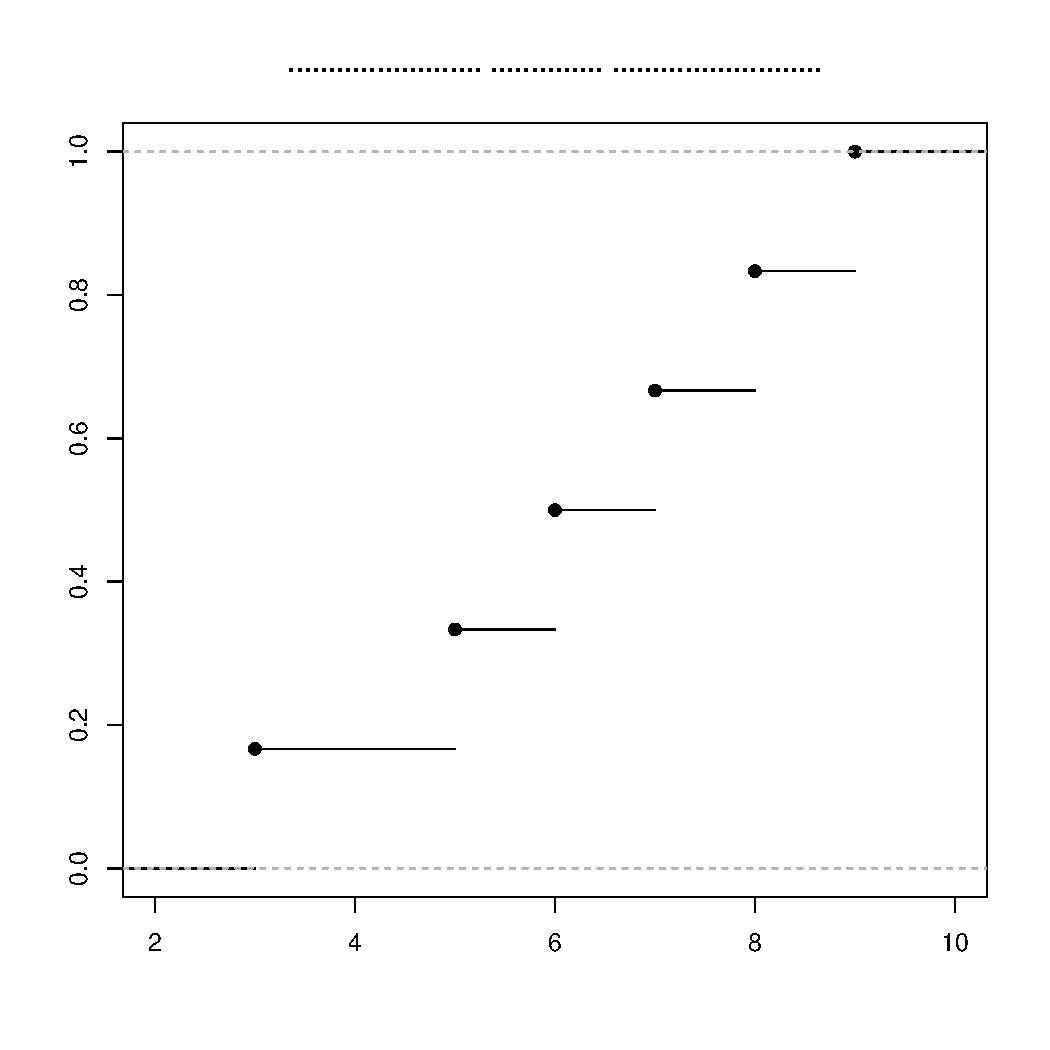
\includegraphics[width=\maxwidth]{figure/empirical_cdf-1} 


\begin{figure}
\begin{tikzpicture}[scale = 0.025]
  % Created by tikzDevice version 0.10.1 on 2017-08-29 12:28:48
% !TEX encoding = UTF-8 Unicode
\definecolor{fillColor}{RGB}{255,255,255}
\path[use as bounding box,fill=fillColor,fill opacity=0.00] (0,0) rectangle (505.89,505.89);
\begin{scope}
\path[clip] (  0.00,  0.00) rectangle (505.89,505.89);
\definecolor{drawColor}{RGB}{0,0,0}

\path[draw=drawColor,line width= 0.4pt,line join=round,line cap=round] ( 74.47, 73.44) -- (460.22, 73.44);

\path[draw=drawColor,line width= 0.4pt,line join=round,line cap=round] ( 74.47, 73.44) -- ( 74.47, 66.24);

\path[draw=drawColor,line width= 0.4pt,line join=round,line cap=round] (170.91, 73.44) -- (170.91, 66.24);

\path[draw=drawColor,line width= 0.4pt,line join=round,line cap=round] (267.34, 73.44) -- (267.34, 66.24);

\path[draw=drawColor,line width= 0.4pt,line join=round,line cap=round] (363.78, 73.44) -- (363.78, 66.24);

\path[draw=drawColor,line width= 0.4pt,line join=round,line cap=round] (460.22, 73.44) -- (460.22, 66.24);

\node[text=drawColor,anchor=base,inner sep=0pt, outer sep=0pt, scale=  1.00] at ( 74.47, 47.52) {2};

\node[text=drawColor,anchor=base,inner sep=0pt, outer sep=0pt, scale=  1.00] at (170.91, 47.52) {4};

\node[text=drawColor,anchor=base,inner sep=0pt, outer sep=0pt, scale=  1.00] at (267.34, 47.52) {6};

\node[text=drawColor,anchor=base,inner sep=0pt, outer sep=0pt, scale=  1.00] at (363.78, 47.52) {8};

\node[text=drawColor,anchor=base,inner sep=0pt, outer sep=0pt, scale=  1.00] at (460.22, 47.52) {10};

\path[draw=drawColor,line width= 0.4pt,line join=round,line cap=round] ( 59.04, 87.27) -- ( 59.04,433.02);

\path[draw=drawColor,line width= 0.4pt,line join=round,line cap=round] ( 59.04, 87.27) -- ( 51.84, 87.27);

\path[draw=drawColor,line width= 0.4pt,line join=round,line cap=round] ( 59.04,156.42) -- ( 51.84,156.42);

\path[draw=drawColor,line width= 0.4pt,line join=round,line cap=round] ( 59.04,225.57) -- ( 51.84,225.57);

\path[draw=drawColor,line width= 0.4pt,line join=round,line cap=round] ( 59.04,294.72) -- ( 51.84,294.72);

\path[draw=drawColor,line width= 0.4pt,line join=round,line cap=round] ( 59.04,363.87) -- ( 51.84,363.87);

\path[draw=drawColor,line width= 0.4pt,line join=round,line cap=round] ( 59.04,433.02) -- ( 51.84,433.02);

\node[text=drawColor,rotate= 90.00,anchor=base,inner sep=0pt, outer sep=0pt, scale=  1.00] at ( 41.76, 87.27) {0.0};

\node[text=drawColor,rotate= 90.00,anchor=base,inner sep=0pt, outer sep=0pt, scale=  1.00] at ( 41.76,156.42) {0.2};

\node[text=drawColor,rotate= 90.00,anchor=base,inner sep=0pt, outer sep=0pt, scale=  1.00] at ( 41.76,225.57) {0.4};

\node[text=drawColor,rotate= 90.00,anchor=base,inner sep=0pt, outer sep=0pt, scale=  1.00] at ( 41.76,294.72) {0.6};

\node[text=drawColor,rotate= 90.00,anchor=base,inner sep=0pt, outer sep=0pt, scale=  1.00] at ( 41.76,363.87) {0.8};

\node[text=drawColor,rotate= 90.00,anchor=base,inner sep=0pt, outer sep=0pt, scale=  1.00] at ( 41.76,433.02) {1.0};

\path[draw=drawColor,line width= 0.4pt,line join=round,line cap=round] ( 59.04, 73.44) --
	(475.65, 73.44) --
	(475.65,446.85) --
	( 59.04,446.85) --
	( 59.04, 73.44);
\end{scope}
\begin{scope}
\path[clip] (  0.00,  0.00) rectangle (505.89,505.89);
\definecolor{drawColor}{RGB}{0,0,0}

\node[text=drawColor,anchor=base,inner sep=0pt, outer sep=0pt, scale=  1.20] at (267.35,471.40) {\bfseries Эмпирическая функция распределения};
\end{scope}
\begin{scope}
\path[clip] ( 59.04, 73.44) rectangle (475.65,446.85);
\definecolor{drawColor}{RGB}{0,0,0}

\path[draw=drawColor,line width= 0.4pt,line join=round,line cap=round] ( 26.25, 87.27) -- (122.69, 87.27);

\path[draw=drawColor,line width= 0.4pt,line join=round,line cap=round] (122.69,144.90) -- (219.13,144.90);

\path[draw=drawColor,line width= 0.4pt,line join=round,line cap=round] (219.13,202.52) -- (267.34,202.52);

\path[draw=drawColor,line width= 0.4pt,line join=round,line cap=round] (267.34,260.14) -- (315.56,260.14);

\path[draw=drawColor,line width= 0.4pt,line join=round,line cap=round] (315.56,317.77) -- (363.78,317.77);

\path[draw=drawColor,line width= 0.4pt,line join=round,line cap=round] (363.78,375.40) -- (412.00,375.40);

\path[draw=drawColor,line width= 0.4pt,line join=round,line cap=round] (412.00,433.02) -- (505.89,433.02);
\definecolor{fillColor}{RGB}{0,0,0}

\path[draw=drawColor,line width= 0.4pt,line join=round,line cap=round,fill=fillColor] (122.69,144.90) circle (  2.70);

\path[draw=drawColor,line width= 0.4pt,line join=round,line cap=round,fill=fillColor] (219.13,202.52) circle (  2.70);

\path[draw=drawColor,line width= 0.4pt,line join=round,line cap=round,fill=fillColor] (267.34,260.14) circle (  2.70);

\path[draw=drawColor,line width= 0.4pt,line join=round,line cap=round,fill=fillColor] (315.56,317.77) circle (  2.70);

\path[draw=drawColor,line width= 0.4pt,line join=round,line cap=round,fill=fillColor] (363.78,375.40) circle (  2.70);

\path[draw=drawColor,line width= 0.4pt,line join=round,line cap=round,fill=fillColor] (412.00,433.02) circle (  2.70);
\definecolor{drawColor}{gray}{0.70}

\path[draw=drawColor,line width= 0.4pt,dash pattern=on 4pt off 4pt ,line join=round,line cap=round] ( 59.04, 87.27) -- (475.65, 87.27);

\path[draw=drawColor,line width= 0.4pt,dash pattern=on 4pt off 4pt ,line join=round,line cap=round] ( 59.04,433.02) -- (475.65,433.02);
\end{scope}

\end{tikzpicture}
\end{figure}
\end{enumerate}

\subsection{Демо-версия зачёта}

\begin{enumerate}
\item Двое подельников, Маша и Саша, украли десять миллионов евро. Через некоторое время Саша был найден убитым, а Маша была арестована. Из свидетельских показаний ясно следует, что Маша и Саша ругались по поводу делёжки. Защита и обвинение выясняют, убила ли Маша Сашу. Из статистических данных известно, что:
\begin{enumerate}
\item[A] 20\% подельников-мужчин ругаются по поводу делёжки
\item[B] 20\% оставшихся в живых подельников-мужчин ругаются по поводу делёжки
\item[C] 5\% мужчин убивают
\item[D] 3\% мужчин убивают их подельники
\item[E] 90\% убитых мужчин-подельников ругались по поводу делёжки
\end{enumerate}
Располагая этой информацией,
\begin{enumerate}
\item Найдите вероятность того, что Маша убила Сашу, если известно, что Маша и Саша ругались по поводу делёжки.
\item Найдите вероятность того, что Маша убила Сашу, если известно, что Маша и Саша ругались по поводу делёжки, и Саша был найден убитым.
\end{enumerate}


\item Маша подкидывает 300 игральных кубиков. Те, что выпали не на шестёрку, она перекидывает один раз. Обозначим буквой $N$ количество шестёрок на всех кубиках после возможных перекидываний.
\begin{enumerate}
\item Найдите $\E(N)$, $\Var(N)$
\item Какова примерно вероятность того, величина $N$ лежит от 50 до 70?
\item Укажите любой интервал, в который величина $N$ попадает с вероятностью 0.9
\end{enumerate}

\item На лукоморье набегают волны. Кот Учёный заметил, что размер каждой волны, $X_i$, — случайная величина, имеющая равномерное распределение от 0 до 1, а размеры волн независимы. Кот Учёный считает волну \textit{большой}, если она больше предыдущей и следующей. Случайная величина $R_i$ равна 1, если $i$-ая волна была \textit{большой}, и 0 иначе.
\begin{enumerate}
\item Найдите $\P(R_i=1)$, $\E(X_i)$
\item Найдите $\E(X_i \mid R_i=1)$
\item Найдите $\Cov(R_1,R_2)$, $\Cov(R_1,R_3)$
\end{enumerate}
\item Ермолай Лопахин решил приступить к вырубке вишневого сада. Однако выяснилось, что растут в нём не только вишни, но и яблони. Причём, по словам Любови Андреевны Раневской, среднее количество деревьев (а они периодически погибают от холода или жары, либо из семян вырастают новые) в саду распределено в соответствии с нормальным законом ($X$ — число яблонь, $Y$ — число вишен) со следующими параметрами:
\begin{equation*}
\begin{pmatrix}	X \\ 	Y 	\end{pmatrix}
\sim \mN
\left(
\begin{pmatrix}
25 \\ 125
\end{pmatrix}
;
\begin{pmatrix}
    5 & 4 \\
    4 & 10
    \end{pmatrix}
\right)
\end{equation*}

\begin{enumerate}
\item Найдите вероятность того, что Ермолаю Лопахину придется вырубить более 150~деревьев.
\item Каково ожидаемое число подлежащих вырубке вишен, если известно, что предприимчивый и последовательный Лопахин, не затронув ни одного вишнёвого дерева, начал очистку сада с яблонь и все 35~яблонь уже вырубил? Какова при этом вероятность того, что Лопахину придется вырубить более 100 вишен?
\end{enumerate}

\item Вопрос из интервью в Морган-Стэнли. Есть две независимых равномерных на отрезке $[0;1]$ случайных величины, $X$ и $Y$. Как их нужно преобразовать, чтобы корреляция между ними оказалась равна $\rho$?
\end{enumerate}

\subsection{Зачёт, 15.01.2013}


\begin{enumerate}
\item Самолёт упал либо в горах, либо на равнине. Вероятность того, что самолёт упал в горах, равна 0.75. Для поиска пропавшего самолёта выделено 3 вертолёта. Каждый вертолёт можно использовать только в одном месте. Как распределить имеющиеся вертолёты, если вероятность обнаружения пропавшего самолёта отдельно взятым вертолётом равна $0.6$?

\item Совместная функция плотности величин $X$ и $Y$ имеет вид
\[
f(x,y)=\frac{1}{x}e^{-x},\: \text{при}\: 0<y<x
\]

\begin{enumerate}
\item Найдите $\P\left( \frac{Y}{X}<0.7 \right)$
\item Найдите $\E(X)$
\item Являются ли $X$ и $Y$ независимыми?
\item Как распределена величина $Z=Y/X$?
\end{enumerate}

\item Величины $X_1$, \ldots, $X_n$ независимы и имеют биномиальное распределение, $X_i \sim Bin(10,p)$. Используя неравенство Чебышёва найдите наименьшее число $t$, чтобы выполнялось условие
\[
\P( | \bar{X}-\E(\bar{X}) | \geq t )\leq 0.01
\]



\item Допустим, что срок службы пылесоса имеет экспоненциальное распределение. В среднем один
пылесос бесперебойно работает 10 лет. Завод предоставляет гарантию 7 лет на свои изделия.
Предположим для простоты, что все потребители соблюдают условия гарантии.
\begin{enumerate}
\item Какой процент потребителей в среднем обращается за гарантийным ремонтом?
\item Какова вероятность того, что из 1000 потребителей за гарантийным ремонтом обратится
более 55\% покупателей?
\end{enumerate}
Подсказка: $\ln 2\approx 0.7$

\item Вася попадает мячом в корзину с вероятностью $0.2$, Петя — с вероятностью $0.25$. Каждый из них сделал по 100 бросков мяча.
\begin{enumerate}
\item Какова вероятность того, что Петя попал на 10 раз больше Васи?
\item Какое минимальное количество бросков мяча нужно сделать каждому, чтобы вероятность, того, что Петя попал на 10 раз больше Васи достигла 0.99?
\end{enumerate}
\end{enumerate}

\subsection{КоКо, компьютерная контрольная №3, 13.03.13}

Продолжительность 1 час 10 минут, разрешено пользоваться конспектами, книжками, заготовками программ, нельзя общаться, использовать Интернет. Текст работы в группах с R:

\begin{enumerate}
\item Величины $X$ и $Y$ независимы. Величина $X$ распределена нормально, $X\sim \cN(4.3,6.7)$, величина $Y$ распределена экспоненциально, $Y\sim \exp(\lambda=2.3)$. Используя симуляционный подход примерно посчитайте

\begin{enumerate}
\item $\P(X+Y>5.6)$
\item $\E(X/(X+5Y))$
\item $\Var(XY)$
\item $\Cov(XY,X/Y)$
\end{enumerate}

\item Загрузите данные по стоимости квартир в Москве, \href{http://goo.gl/zL5JQ}{goo.gl/zL5JQ}, в табличку с именем \verb|h|. Обозначим буквой \verb|a| ответ на первый вопрос первой задачи. Отберите индивидуальную выборку лично для себя, выполнив команды:
\begin{knitrout}
\definecolor{shadecolor}{rgb}{0.969, 0.969, 0.969}\color{fgcolor}\begin{kframe}
\begin{alltt}
\hlkwd{set.seed}\hlstd{(}\hlkwd{round}\hlstd{(}\hlnum{100} \hlopt{*} \hlstd{a))} \hlcom{# здесь "a" — это ответ на первый пункт первой задачи}
\hlstd{h} \hlkwb{<-} \hlstd{h[}\hlkwd{sample}\hlstd{(}\hlnum{1}\hlopt{:}\hlkwd{nrow}\hlstd{(h),} \hlnum{1000}\hlstd{), ]}
\end{alltt}
\end{kframe}
\end{knitrout}

Постройте 90\%-ый доверительный интервал для:
\begin{enumerate}
\item Доли кирпичных домов, \verb|brick==1|
\item Доли кирпичных домов, \verb|brick==1|, среди домов находящихся близко от метро,  \verb|walk==1|
\item Разницы доли кирпичных домов среди домов расположенных близко и далеко от метро
\end{enumerate}


\item Сгенерируйте искусственные данные, выполнив команды:
\begin{knitrout}
\definecolor{shadecolor}{rgb}{0.969, 0.969, 0.969}\color{fgcolor}\begin{kframe}
\begin{alltt}
\hlkwd{set.seed}\hlstd{(}\hlkwd{round}\hlstd{(}\hlnum{100} \hlopt{*} \hlstd{a)} \hlopt{+} \hlnum{42}\hlstd{)} \hlcom{# здесь "a" — это ответ на первый пункт первой задачи}
\hlstd{x} \hlkwb{<-} \hlkwd{rexp}\hlstd{(}\hlnum{200}\hlstd{,} \hlkwc{rate} \hlstd{=} \hlnum{2}\hlstd{)}
\end{alltt}
\end{kframe}
\end{knitrout}

Величины $X_i$ независимы и имеют функцию плотности $f(x)=e^{b-xe^b}$ при $x>0$.
\begin{enumerate}
\item Оцените неизвестный параметр $b$
\item Оцените дисперсию полученной оценки
\item Постройте 90\%-ый доверительный интервал для $b$
\item Используя результат предыдущего пункта, на 10\%-ом уровне значимости проверьте гипотезу $H_0$: $b=0.7$ против альтернативной гипотезы $H_a$: $b\neq 0.7$.
\end{enumerate}

\end{enumerate}


\subsection{Экзамен, 26.03.2013}


\begin{enumerate}
%в комментариях предполагаемые ответы


\item Вероятность выигрыша по лотерейному билету равна $0.05$. Вероятность того, что из трёх купленных билетов ровно два окажутся выигрышными примерно равна

\otvet{0.002}{0.0025}{0.007}{0.1}{0.3}

\item Закон распределения случайной величины задан табличкой

\begin{tabular}{@{}cccc@{}}
\toprule
$X$         & $-1$  & $0$   & $1$ \\ \midrule
$\P(\cdot)$ & $0.4$ & $0.2$ & ?   \\ \bottomrule
\end{tabular}

Дисперсия величины $X$, $\Var(X)$, равняется

\otvet{0}{0.02}{0.3}{0.8}{2}

%3
\item Если $f(x)$ — функция плотности, то $\int_{-\infty}^{x}f(u)\,du$ равен

\otvet{0}{1}{$\E(X)$}{$\Var(X)$}{$F(x)$}

%4
\item События $A$ и $B$ называются независимыми, если

\lotvet{$\P(A\cup B)=\P(A)+\P(B)$}
{$\P(A)\cdot\P(B)=\P(A\cap B)$}
{$\P(A\cup B)=\P(A)+\P(B)-\P(A\cap B)$}
{$\P(A\cap B)=0$}
{нет верного} \\ \\

%5
\item Правильную монетку подбрасывают два раза. Рассмотрим два события: $A$ — при втором броске выпала «решка», $B$ — «орёл» выпал хотя бы один раз. Найдите $\P(A|B)$

\otvet{0}{1/3}{1/2}{2/3}{1}

%6
\item Есть пять случайных величин: $X\sim \chi^2_{10}$, $Y\sim F_{5,10}$, $T\sim t_{10}$, $Z\sim \cN(0,1)$, $W\sim \cN(10,1)$. Какие из величин распределены симметрично относительно 0?

\otvet {X, Y, Z}{Z, W}{Z, T}{Z}{X, Y}

%7
\item Известно, что $\E(X)=3$, $\Var(X)=1$, $\E(Y)=4$, $\Var(Y)=9$, $\E(XY)=13$, найдите $\Cov(X,Y)$

\otvet{0}{-3}{18}{3}{1}

%8
\item Известно, что $\E(X)=3$, $\Var(X)=1$, $\E(Y)=4$, $\Var(Y)=9$, $\E(XY)=6$, найдите $\Var(2X+Y)$

\otvet{13}{7}{1}{17}{нет верного ответа}

%9
\item Если $F(x)$ — это функция распределения, то $\lim_{x\to -\infty}F(x)$ равен

\otvet{0}{0.5}{1}{$\E(X)$}{$+\infty$}

%10
\item Если $X\sim \cN(-4;1)$, то $\P(3X+571>0)$ примерно равна

\otvet{0}{0.5}{1}{$+\infty$}{нет верного ответа}

%11
\item Про закон распределения величины $X$ ничего не известно. Укажите самую точную оценку сверху для вероятности $\P(|X-\E(X)|>3\sqrt{\Var(X)})$

\otvet{$0.(3)$}{$0.6(3)$}{$0.(1)$}{$1$}{нет верного ответа}

%12
\item Функция распределения, $F(x)=\P(X\leq x)$ может не являться

\otvet{непрерывной}{непрерывной справа}{монотонно неубывающей}{ограниченной}{неотрицательной}

%13
\item Ковариационной может быть матрица:

\otvet {$\left(\begin{array}{cc}
-1 & 1\\
1 & 2
\end{array}\right)$}{$\left(\begin{array}{cc}
1 & 0.5\\
1 & 2
\end{array}\right)$}{$\left(\begin{array}{cc}
1 & -1\\
-1 & 2
\end{array}\right)$}{$\left(\begin{array}{cc}
-1 & 1\\
1 & -2
\end{array}\right)$}{$\left(\begin{array}{cc}
1 & 1\\
-0.7 & 2
\end{array}\right)$}\\

%14
\item Если $X$ и $Y$ независимые случайные величины, то неверным может быть утверждение

\lotvet{$\E(X+Y)=\E(X)+\E(Y)$}
{$\E(X/Y)=\E(X)/\E(Y)$}
{$\E(XY)=\E(X)\cdot\E(Y)$}
{$\Var(X+Y)=\Var(X)+\Var(Y)$}
{$\Cov(X,Y)=0$} \\ \\

%15
\item Известно, что  $\Cov(X,Y)=0$, $\Var(X)=10$, $\Var(Y)=10$. \\
Неверным может быть утверждение

\lotvet{$\Corr(X,Y)=0$}
{$\Corr(X+a,Y+b)=0$}
{$\E(X\cdot Y)=\E(X)\cdot \E(Y)$}
{$\Var(X+Y)=\Var(X)+\Var(Y)$}
{$X$ и $Y$ независимы} \\ \\

%16
\item $Z_1,Z_2,\ldots,Z_n\sim\cN(0,1)$. Тогда величина $\frac{Z_1\sqrt{n-2}}{\sqrt{\sum_{i=3}^n Z_i^2}}$ имеет распределение

\otvet {$\cN(0,1)$}{$t_n$}{$F_{1,n-2}$}{$\chi^2_n$}{$t_{n-2}$}

%17
\item Количество страниц в книгах авторов $X$ и $Y$ распределено нормально с дисперсиями $\sigma^2_X$ и $\sigma^2_Y$ соответственно. Для тестирования гипотезы о равенстве дисперсий было выбрано $n$ книг автора $X$ и $m$ книг — автора $Y$. Какое распределение имеет статистика, используемая в данном случае?

\otvet {$\chi^2_{\min(m,n)}$}{$\chi^2_{\max(m,n)}$}{$F_{m,n}$}{$F_{m-1,n-1}$}{$F_{m+1,n+1}$}

%18
\item Если величина $X$ имеет $\chi^2_k$-распределение, величина $Y$ — $\chi^2_n$-распределение, и они независимы, то дробь $nX/(kY)$ имеет распределение

\otvet{$F_{k,n}$}{$F_{n,k}$}{$F_{k-1,n-1}$}{$\chi^2_{n-k}$}{$F_{n-1,k-1}$}

%19
\item \emph{Смещённой} оценкой математического ожидания по выборке независимых,
одинаково распределенных случайных величин $X_1$, $X_2$, $X_3$ является оценка

\lotvet{$(X_1+X_2)/2$}{$(X_1+X_2+X_3)/3$}{$0.7X_1+0.2X_2+0.1X_3$}{$0.3X_1+0.3X_2+0.3X_3$}{$X_1+X_2-X_3$} \\ \\

%20
\item Если величины $X$ и $Y$ независимы и равномерно распределены на $[0;1]$, а $F(x,y)$ — их совместная функция  распределения, то $F(0.5,3)$ равно

\otvet{0}{0.5}{1}{1.5}{не существует}

%21
\item Если $X_i$ независимы и имеют нормальное распределение $\cN(-1;2013)$, то $\sqrt{n}(1+\bar{X})/\hat{\sigma}$ имеет распределение

\otvet{$\cN(0;1)$}{$t_{n-1}$}{$\chi^2_{n-1}$}{$\cN(0;2013/n)$}{$t_n$}

%22
\item Последовательность оценок $\hat{\theta}_1$, $\hat{\theta}_2$, \ldots называется состоятельной, если

\lotvet{$\E(\hat{\theta}_n)=\theta$}{$\Var(\hat{\theta}_n)\to 0$}{$\P(|\hat{\theta}_n - \theta |>t)\to 0$ для всех $t>0$}{$\E(\hat{\theta}_n)\to \theta$}
{$\Var(\hat{\theta}_n)\geq \Var(\hat{\theta}_{n+1})$} \\ \\

%23
\item Величины $X_1$, \ldots, $X_5$ равномерны на отрезке $[0;a]$. Известно, что $\sum_{i=1}^5 x_i=25$. При использовании первого момента оценка методом моментов неизвестного $a$ равна

\otvet{1}{5}{10}{20}{нет верного ответа}

%24
\item При построении доверительного интервала для отношения дисперсий по двум независимым нормальным выборкам из $n$ наблюдений каждая, используется статистика, имеющая распределение

\otvet{$F_{n-1,n-1}$}{$t_{n-1}$}{$\chi^2_{n-1}$}{$\chi^2_{n}$}{$t_n$}

%25
\item Ботаники\footnote{В отличие от ботаников, зоологи точно знают, сколько иголок у ёжиков!} строят доверительный интервал для математического ожидания числа иголок у ёжа. Количество иголок на одном еже предполагается нормально распределенным. Среднее число иголок у пойманных 100 ёжиков равно 1500, выборочная дисперсия — 400. На 5\% уровне значимости какой примерно доверительный интервал должны построить ботаники?


\lotvet {$[1499;1501]$}{$[1498;1502]$}{$[1497;1503]$}{$[1496;1504]$}{нет верного ответа}\\ \\

%26
\item Функция правдоподобия, построенная по случайной выборке $X_1$, \ldots, $X_n$ из распределения с функцией плотности $f(x)=(\theta+1)x^{\theta}$ при $x\in [0;1]$ имеет вид

\otvet{$(\theta+1)x^{n\theta}$}{$\sum (\theta+1)x_i^{\theta}$}
{$(\theta+1)^{\sum x_i}$}{$(\sum x_i)^{\theta}$}{$(\theta+1)^n\prod x_i^{\theta}$}

%27
\item Если $X_i$ независимы, $\E(X_i)=\mu$ и $\Var(X_i)=\sigma^2$, то математическое ожидание величины $Y=\sum_{i=1}^{n}(X_i-\bar{X})^2$ равно

\otvet{$\hat{\sigma}^2$}{$(n-1)\sigma^2$}{$\mu$}{$\sigma^2$}{$\sigma^{2}/n$}

%28
\item Если $P$-значение меньше уровня значимости $\alpha$, то гипотеза $H_0$: $\sigma=\sigma_0$

\lotvet{отвергается}{не отвергается}{отвергается только если $H_a$: $\sigma \neq \sigma_0$}{отвергается только если $H_a$: $\sigma<\sigma_0$}{недостаточно информации} \\

\item Если $H_0$ верна, то $P$-значение имеет распределение

\otvet{$U[0;1]$}{$\cN(0,1)$}{$t_n$}{$t_{n-1}$}{$\chi^2_{n-1}$}


\end{enumerate}




\textbf{Экзамен по теории вероятностей! Суперигра!}

\vspace{20pt}
\begin{center}
\textbf{DON'T PANIC}
\end{center}
\vspace{20pt}


\begin{enumerate}
\item В группе учится 30 студентов, 20 девушек и 10 юношей. Они входят в аудиторию в случайном порядке. Рассчитайте вероятности событий:
\begin{enumerate}
\item Маша Петрова\footnote{Маша Петрова — единственная и неподражаемая!} войдёт девятой по счёту
\item Девятый вошедший окажется девушкой
\item Перед Машей Петровой войдут ровно 5 юношей
\item Перед Машей Петровой войдут ровно 5 юношей, если известно, что Маша Петрова вошла девятой
\item Маша Петрова войдёт девятой по счёту, если известно, что перед ней вошло ровно 5 юношей
\end{enumerate}

\item В поселке 2500 жителей. Каждый из них в среднем 6 раз в месяц ездит в город, выбирая день поездки независимо от других людей. Поезд ходит в город один раз в сутки.
\begin{enumerate}
\item Какой наименьшей вместимостью должен обладать поезд, чтобы он переполнялся в среднем не чаще 1 раза в 100 дней?
\item Сколько в среднем человек будет ехать в таком поезде, если предположить, что при переполнении часть людей полностью откажется от поездки?
\end{enumerate}

Источник: экзамен РЭШ

\item Случайные величины $X_1$, $X_2$, \ldots, $X_n$ независимы и имеют пуассоновское распределение с неизвестным параметром $\lambda$.
\begin{enumerate}
\item С помощью метода максимального правдоподобия постройте оценки для $\lambda$ и для $\exp(\lambda)$
\item Предположим, что исследователь не знает, чему равны $X_i$. Ему известно лишь, равно ли каждое из $X_i$ нулю или нет. С помощью метода максимального правдоподобия постройте оценки для $\lambda$ и для $\exp(\lambda)$. Всегда ли существуют предложенные оценки?
\end{enumerate}


\item В таблице представлены данные по количеству пассажиров «Титаника», поделенные на группы по классу каюты:

% latex table generated in R 3.4.2 by xtable 1.8-2 package
% Fri Oct 27 14:26:27 2017
\begin{table}[ht]
\centering
\begin{tabular}{rrrr}
  \hline
 & 1 класс & 2 класс & 3 класс \\ 
  \hline
Погиб & 122 & 167 & 528 \\ 
  Выжил & 203 & 118 & 178 \\ 
   \hline
\end{tabular}
\end{table}


Проверьте гипотезу о независимости шансов выжить от класса каюты.

\item Перед Вами две внешне неотличимых монетки. Одна из них выпадает «орлом» вверх с вероятностью $0.7$, другая — с вероятностью $0.3$. Вы имеете право на 4 подбрасывания. Перед каждым подбрасыванием Вы можете выбирать подбрасываемую монетку. За каждого выпавшего «орла» вы получаете 1 рубль.
\begin{enumerate}
\item Какова оптимальная стратегия?
\item Каков ожидаемый выигрыш при использовании оптимальной стратегии?
\end{enumerate}

\end{enumerate}

\section{2013-2014}

\section{2013-2014}

\subsection{Контрольная работа №1, 5.11.2013}

\begin{enumerate}
\item Вероятность застать Васю на лекции зависит от того, пришли ли на лекцию Маша и Алена. Данная вероятность равна $0.18$, если девушек нет; $0.9$ — если обе девушки пришли на лекцию; $0.54$ — если пришла только Маша и $0.36$ — если пришла только Алена. Маша и Алена посещают лекции независимо друг от друга с вероятностями $0.4$ и $0.6$ соответственно.
\begin{enumerate}
\item Определите вероятность того, что на лекции присутствует Алена, если в аудитории есть Вася.
\item Кого чаще можно застать на тех лекциях, на которых присутствует Вася: Машу или Алену?
%\item При каком значении $p$ Вася посещает половину всех лекций?
\end{enumerate}


\item Страховая компания страхует туристов, выезжающих за границу, от невыезда и наступления страхового медицинского случая за границей. Застраховано 100 туристов. Вероятность «невыезда» за границу случайно выбранного туриста — $0.002$, а страховые выплаты в этом случае — 2000 у.е.; вероятность обращения за медицинской помощью за границей — $0.01$, а страховые выплаты — 3000 у.е. Для каждого туриста рассмотрим две случайные величины: $X_i$, равную 1 при невыезде за границу и 0 иначе, и $Y_i$, равную 1 при обращении за медицинской помощью и нулю иначе. Обозначим $X=\sum_{i=1}^{100}X_i$ и $Y=\sum_{i=1}^{100}Y_i$.
\begin{enumerate}
\item Определите $\P(X=5)$, $\E(X)$, $\Var(X)$
\item Наиболее вероятное число не выехавших туристов.
\item Вычислите математическое ожидание и дисперсию величины совокупных страховых выплат
\end{enumerate}
Подсказка: Число обращений в страховую компанию для каждого туриста может быть записано в виде $X_i+X_i Y_i$, так как медицинский страховой случай может наступить только, если турист выехал за границу. Случайные величины $X_i$ и $Y_i$ независимы.

\item Функция плотности случайной величины $X$ имеет вид:
\begin{equation}
f(x)=\begin{cases}
ce^{-x}, \, x\geq 0 \\
ce^x, \, x<0
\end{cases}
\end{equation}
\begin{enumerate}
\item Найдите $c$, $\P(X \in [\ln 0.5,\ln 4])$, $\E(X)$, $\Var(X)$
\item Моменты всех порядков случайной величины $x$
\end{enumerate}

Подсказка: $\int_0^{\infty} x^n e^{-x} \, dx=n!$

\item Известно, что  $\E(X)=-1$, $\E(Y)=1$, $\Var(X)=9$, $\Var(Y)=4$, $\Corr(X,Y)=1$. Найдите
\begin{enumerate}
\item $\E(Y-2X-3)$, $\Var(Y-2X-3)$
\item  $\Corr(Y-2X-3,X)$
\item Можно ли выразить $Y$ через $X$? Если да, то запишите уравнение связи.
\end{enumerate}

\item Совместное распределение доходов акций двух компаний $Y$ и $X$ задано в виде таблицы

\begin{tabular}{c|ccc}
 & $X=-1$ & $X=0$ & $X=1$ \\
\hline
$Y=-1$ & $0.1$ & $0.2$ & $0.2$ \\
$Y=1$ & $0.2$ & $0.1$ & $0.2$ \\
\end{tabular}


\begin{enumerate}
\item Найдите  частные распределения случайных величин $X$ и $Y$
\item Найдите $\Cov(X,Y)$
\item Можно ли утверждать, что случайные величины $X$ и $Y$ зависимы?
\item Найдите условное распределение случайной величины $X$ при условии $Y=-1$
\item Найдите условное математическое ожидание $\E(X\mid Y=-1)$
\end{enumerate}


\end{enumerate}

Некоторые ответы:
\begin{enumerate}
\item xx
\item $\P(X=5)=C_{100}^5 0.002^5 0.998^{95}$, $\E(X)=0.2$, $\Var(X)=0.2\cdot 0.998$, наиболее вероятно событие $X=0$
\item $c=1/2$, $P=5/8$, $\E(X)=0$, $\Var(X)=2$, $\E(X^{2k+1})=0$, $\E(X^{2k})=(2k)!$
\item xx
\item xx
\end{enumerate}



\subsection{Контрольная работа №1, i-поток, 15.11.2013}

\subsubsection*{Часть 1}

\begin{enumerate}

\item В жюри три человека, они должны одобрить или не одобрить конкурсанта. Два члена жюри независимо друг от друга одобряют конкурсанта с одинаковой вероятностью $p$. Третий член жюри  для вынесения решения бросает правильную монету. Окончательное решение выносится большинством голосов.
\begin{enumerate}
\item С какой вероятностью жюри одобрит конкурсанта?
\item Что выгоднее для  конкурсанта: чтобы решение принимало данное жюри, или чтобы решение принимал один человек, одобряющий с вероятностью $p$?
\end{enumerate}


\item Вероятность застать Васю на лекции зависит от того, пришли ли на лекцию Маша и Алена. Данная вероятность равна $p$, если девушек нет; $5p$ — если обе девушки пришли на лекцию; $3p$ — если пришла только Маша и $2p$ — если пришла только Алена. Маша и Алена посещают лекции независимо друг от друга с вероятностями $0.6$ и $0.3$ соответственно.
\begin{enumerate}
\item Определите вероятность того, что на лекции присутствует Алена, если в аудитории есть Вася.
\item Кого чаще можно застать на тех лекциях, на которых присутствует Вася: Машу или Алену?
\item При каком значении $p$ Вася посещает половину всех лекций?
\end{enumerate}

\item Страховая компания страхует туристов, выезжающих за границу, от невыезда и наступления страхового медицинского случая за границей. Застраховано 100 туристов. Вероятность «невыезда» за границу случайно выбранного туриста — $0.002$, а страховые выплаты в этом случае — 2000 у.е.; вероятность обращения за медицинской помощью за границей — $0.01$, а страховые выплаты — 3000 у.е.
\begin{enumerate}
\item Определите вероятность того, что ровно пятеро туристов не смогут выехать за границу.
\item Найдите математическое ожидание, дисперсию и наиболее вероятное число не выехавших туристов.
\item Вычислите математическое ожидание и дисперсию величины совокупных страховых выплат
\item Вычислите ковариацию между выплатами по двум видам страхования.
\end{enumerate}

\item Известно, что  $\E(X)=-1$, $\E(Y)=1$, $\Var(X)=9$, $\Var(Y)=4$, $\Corr(X,Y)=1$. Найдите
\begin{enumerate}
\item $\E(Y-2X-3)$, $\Var(Y-2X-3)$
\item  $\Corr(Y-2X-3,X)$
\item Можно ли выразить $Y$ через $X$? Если да, то запишите уравнение связи.
\end{enumerate}

Решение: корреляция равна 1, значит есть линейная взаимосвязь между переменными. Пусть $Y+\beta X=const$, тогда $\Var(Y+\beta X)=0$. Решая уравнение находим, что $\beta=-2/3$.

\item Совместное распределение доходов акций двух компаний $Y$ и $X$ задано в виде таблицы

\begin{tabular}{c|ccc}
 & $X=-1$ & $X=0$ & $X=1$ \\
\hline
$Y=-1$ & $0.1$ & $0.2$ & $0.2$ \\
$Y=1$ & $0.2$ & $0.1$ & $0.2$ \\
\end{tabular}

Найдите:
\begin{enumerate}
\item Частные распределения случайных величин $X$ и $Y$
\item $\Cov(X,Y)$
\item Можно ли утверждать, что случайные величины $X$ и $Y$ зависимы?
\item У инвестора портфель, в котором доля акций $X$ составляет $
\alpha$, а доля акций $Y$ — $(1-\alpha)$. Каковы должны быть доли, чтобы риск портфеля (дисперсия дохода) был бы минимальным?
\item Условное распределение случайной величины $X$ при условии $Y=-1$
\item Условное математическое ожидание $\E(X\mid Y=-1)$
\end{enumerate}

\item Докажите, что из сходимости в среднем порядка $s>0$ следует сходимость по вероятности.

\end{enumerate}


\subsubsection*{Часть 2}

\begin{enumerate}

\item Муравей находится внутри спичечного коробка, в вершине $A$. В противоположной вершине $B$ есть маленькая дырочка, через которую муравей сможет выбраться на поверхность. В вершине $C$, соседней с вершиной $A$, лежит крупинка сахара. Муравей ползает только по рёбрам коробка, выбирая каждый раз равновероятно одно из доступных в вершине рёбер наугад. Например, он может поползти обратно.
\begin{enumerate}
\item Какова вероятность того, что муравей найдет крупинку сахара до того, как выберется?
\item Сколько в среднем перемещений понадобится муравью, чтобы выбраться?
\item Какова дисперсия количества перемещений, которые понадобятся муравью, чтобы выбраться?
\end{enumerate}

\item В очереди стояло $20$ человек, когда касса внезапно закрылась. Поэтому $10$ случайных людей из очереди решили покинуть очередь. В результате этого очередь оказалась разбита на случайное число кусков $X$. Найдите $\E(X)$, $\Var(X)$.

\item Предположим, что три возможных генотипа \verb|aa|, \verb|Aa| и \verb|AA| изначально встречаются с частотами $p_1$, $p_2$ и $p_3$, где $p_1+p_2+p_3=1$. Ген не сцеплен с полом, поэтому частоты $p_1$, $p_2$ и $p_3$ одинаковы для мужчин и для женщин.
\begin{enumerate}
\item У семейных пар из этой популяции рождаются дети. Назовём этих детей первым поколением. Каковы частоты для трёх возможных генотипов в первом поколении?
\item У семейных пар первого поколения тоже рождаются дети. Назовём этих детей вторым поколением. Каковы частоты для трёх возможных генотипов во втором поколении?
\item Каковы частоты для трёх возможных генотипов в $n$-ном поколении?
\item Заметив явную особенность предыдущего ответа сформулируйте теорему о равновесии Харди-Вайнберга. Прокомментируйте утверждение: «Любой рецессивный ген со временем исчезнет».
\end{enumerate}

\item Световая волна может быть разложена на две поляризованные составляющие, вертикальную и горизонтальную. Поэтому состояние отдельного поляризованного фотона может быть описано\footnote{На самом деле внутренний мир фотона гораздо разнообразнее.} углом $\alpha$. Поляризационный фильтр описывается углом поворота $\theta$. Фотон в состоянии $\alpha$ задерживается поляризационным фильтром с параметром $\theta$ с вероятностью $p=\sin^2(\alpha-\theta)$ или проходит сквозь фильтр с вероятностью $1-p$, переходя при этом в состояние $\theta$.

\begin{enumerate}
\item Какова вероятность того, что поляризованный фотон в состоянии $\alpha$ пройдёт сквозь фильтр с параметром $\theta=0$?
\item Имеется два фильтра и поляризованный фотон в состоянии $\alpha$. Первый фильтр — с $\theta=0$, второй — c $\theta=\pi/2$. Какова вероятность того, что фотон пройдет через оба фильтра?
\item Имеется три фильтра и поляризованный фотон в состоянии $\alpha$. Первый фильтр — с $\theta=0$, второй — c $\theta=\beta$, третий — с $\theta=\pi/2$. Какова вероятность того, что фотон пройдет через все три фильтра? При каких $\alpha$ и $\beta$ она будет максимальной и чему при этом она будет равна?
\item Объясните следующий фокус. Фокусник берет два специальных стекла и видно, что свет сквозь них не проходит. Фокусник ставит между двумя стёклами третье, и свет начинает проходить через три стекла.
\end{enumerate}


\end{enumerate}

Некоторые ответы:
\begin{enumerate}
\item $\P(A)=2/3$
\item $\E(X)=5.5$
\end{enumerate}


\subsection{Контрольная работа №2, i-поток, 16-28.12.2013}

\subsubsection*{Заочная R-часть}

\begin{enumerate}
\item Случайная величина $X$ имеет $t$-распределение с $5$-тью степенями свободы.
\begin{enumerate}
\item На одном графике постройте функцию плотности случайной величины $X$ и функцию плотности стандартного нормального распределения.
\item На одном графике постройте функцию распределения случайной величины $X$ и функцию распределения стандартной нормальной случайной величины.
\item Постройте график зависимости вероятности $\P(a<X<a+10)$ от $a$. Если возможно, найдите такое число $a$, при котором эта вероятность равна $0.8$.
\item Постройте график зависимости вероятности $\P(b<X<2b)$ от $b$ при $b>0$. Если возможно, найдите такое число $b$, при котором эта вероятность равна $0.2$.
\item С помощью $10^6$ симуляций оцените $\P(X^3+X>3)$, $\E(1/(X^2+3))$, $\Var(1/(X^2+3))$.
\item На одном графике постройте гистограмму получившейся случайной выборки из $10^6$ значений и функцию плотности $X$. Для сравнимости гистограммы и функции плотности масштаб гистограммы нужно выбрать так, чтобы площадь под ней равнялась единице.
\item С помощью этой же случайной выборки найдите самый короткий интервал, куда $1/(X^2+1)$ попадает с вероятностью $0.9$.
\end{enumerate}


\item Слагаемые $X_i$ независимы и экспоненциально распределены с параметром $\lambda=2$. Обозначим сумму буквой $S_n$, т.е. $S_n=X_1+\ldots+X_n$.

Для $n=5$, $n=10$, $n=50$, $n=100$:

\begin{enumerate}
\item Сгенерируйте случайную выборку из $10^4$ значений $S_n$.
\item Постройте выборочную функцию распределения $S_n$.
\item Найдите выборочное среднее и выборочную дисперсию $S_n$. Сравните их с настоящим математическим ожиданием $\E(S_n)$ и настоящей дисперсией $\Var(S_n)$.
\item На одном графике в общем масштабе постройте гистограмму для $S_n$ и функцию плотности нормально распределенной случайной величины с математическим ожиданием, равным $\E(S_n)$, и дисперсией, равной $\Var(S_n)$.
\item Оцените по построенной случайной выборке вероятность.
\[ \P(S_n \in [0.5 \sqrt{\Var(S_n)} ; 2\sqrt{\Var(S_n}) ]) \]
\item Оцените ту же вероятность, используя нормальную аппроксимацию.
\item Сравните две полученные оценки вероятности между собой.
\end{enumerate}


\item Вектор $(X,Y)$ имеет совместное нормальное распределение, $\E(X)=\E(Y)=0$, $\Var(X)=1$, $\Var(Y)=9$, $\Corr(X,Y)=\rho$.

Для $\rho=-0.9$, $\rho=0$, $\rho=0.5$:

\begin{enumerate}
\item Найдите ковариационную матрицу вектора  $(X,Y)$, найдите её собственные числа и собственные векторы
\item Постройте график совместной функции плотности
\item Найдите $\P(X\in [0,1], \, Y\in [-2,1] )$
\item Сгенерируйте случайную выборку из $10^3$ пар значений $(X_i,Y_i)$
\item Найдите выборочную ковариацию и выборочную корреляцию между $X_i$ и $Y_i$, сравните их с истинными ковариацией и корреляцией
\item На диаграмме рассеяния дополнительно постройте линии уровня совместной функции плотности $f(x,y)$
\item На диаграмме рассеяния дополнительно постройте собственные векторы с длинной равной корню из соответствующего собственного значения. Каков геометрический смысл собственных векторов ковариационной матрицы?
\item Оцените $\P(Y>X+1)$ двумя способами: с помощью имеющейся случайной выборки и численно взяв интеграл от совместной функции плотности
\end{enumerate}


\item[*] \textit{Необязательная задача}. Вдоль края стоянки идёт неразмеченная парковка длиной 100 метров. Машины приезжают по очереди и паркуются перпендикулярно тротуару на случайное место, выбираемое равномерно из возможных для парковки. Водитель считает место возможным для парковки, если расстояние до машин слева и справа не менее $50$ сантиметров. Ширина автомобиля $1.7$ метра.

Случайная величина $N$ — количество машин, которые смогут припарковаться на данной парковке. С помощью $10^6$ симуляций ответьте на вопросы:
\begin{enumerate}
\item Сколько машин в среднем умещается на парковке?
\item Сколько места при случайной парковке пропадает в среднем «впустую» по сравнению с максимально аккуратной «размеченной» парковкой?
\item Чему равна дисперсия величины $N$?
\item Найдите самый короткий интервал, в который $N$ попадает с вероятностью $0.8$.
\item Похоже ли распределение $N$ на биномиальное? Для ответа на этот вопрос постройте на одном графике выборочную гистограмму для $N$ и гистограмму истинных вероятностей для биномиального распределения со средним и дисперсией равным оценкам среднего и дисперсии для $N$.
\end{enumerate}


\end{enumerate}

Требования к оформлению домашнего задания:
\vspace{0.5cm}
\begin{enumerate}
\item Сдается в распечатанном виде в срок. Отмазки в духе «инопланетяне украли принтер утром, когда всё уже было готово» принимаются только вместе с видео-записью гуманоидов, похищающих принтер.
\item Обязательно использование языка R и пакета \verb|knitr| с автоматическим созданием \verb|pdf|-файла из \verb|Rnw|-файла. Работы со шрифтом Times New Roman будут торжественно сожжены на кафедре до проверки! Код всех команд должен быть открыт для проверки.
\item Работа должна быть написана на русском языке. Do You speak English? Sprechen Sie Deutsch? Parlez-Vous Français?
\item На графиках должны быть подписаны оси. Convincing, \url{http://xkcd.com/833/}.
\item Обязательно в работе должны быть указаны: фамилия, имя, номер группы, e-mail. Необязательно —  номер кредитной карточки с cvv кодом и сроком действия.
\end{enumerate}


\subsubsection*{Очная часть, 25.12.2013}
Самая важная формула:
\[
\frac{1}{\left(\sqrt{2\pi}\right)^n\det(C)}\exp\left(-\frac{1}{2}(x-\mu)'C^{-1}(x-\mu)\right)
\]
Неравенство Берри-Эссеена:
\[
|F_n(x)-\Phi(x)| \leq \frac{C_0 \E|X_1-\mu|^3}{\sigma^3 \sqrt{n}}, \, 0.4<C_0<0.48
\]
\begin{enumerate}

%\item Вася может добраться от метро до института пешком или проехать остановку на трамвае. В среднем Вася ездит  на трамвае один раз за два дня и решение о поездке принимает независимо от того, когда он ездил последний раз. Для простоты предположим, что время между двумя поездками Васи на трамвае распределено экспоненциально.  Перед посадкой в трамвай Вася купил билет на три поездки. Какова вероятность того, что он использует (полностью) этот билет до истечения срока действия (5 дней)?

\item Складываются $n=120$  чисел, каждое из которых округлено с точностью до $0.1$. Предположим, что ошибки округления независимы и равномерно распределены в интервале $(-0.05, 0.05 )$.
\begin{enumerate}
\item Найдите  пределы, в которых с вероятностью не меньшей 0.98  лежит суммарная ошибка.
\item  Вычислите максимальную погрешность, с которой истинная вероятность  попадания в найденный интервал суммарной ошибки округления отличается от 0.98.
\end{enumerate}
Подсказка: Следует искать симметричный относительно нуля интервал.

\item  Театр имеет два различных входа. Около каждого из входов имеется свой гардероб. Эти гардеробы ничем не отличаются. На спектакль приходит 1000 зрителей. Предположим, что зрители приходят поодиночке и выбирают входы равновероятно.
\begin{enumerate}
\item Сколько мест должно быть в каждом из гардеробов для того, чтобы в среднем в 99 случаях из 100 все зрители могли раздеться в гардеробе того входа, через который они вошли?
\item Предположим, что в каждом гардеробе ровно 500 мест. Найдите математическое ожидание числа зрителей, которым придется перейти в другой гардероб.
\end{enumerate}

\item Рост в сантиметрах, $X$, и вес в килограммах, $Y$, взрослого мужчины является двумерным нормальным вектором
$Z=(X,Y)$ с математическим ожиданием $\E(Z)=(175,74)$ и ковариационной матрицей
\[
\Var(Z)=
\begin{pmatrix}
49 & 28 \\
28 & 36
\end{pmatrix}
\]


Лишний вес характеризуется случайной величиной $U=X-Y$. Считается, что человек страдает избыточным весом, если $U<90$.
\begin{enumerate}
\item Определите процент мужчин, чей рост отклоняется от среднего более, чем на 10 см.
\item Определите процент мужчин, чей вес отклоняется от среднего более, чем на 10 кг.
\item Каково распределение величины $U$ ? Выпишите функцию плотности
\item Определите вероятность того, что человек страдает избыточным весом
\item Каково условное распределение веса при фиксированном росте? Выпишите функцию плотности
\item Какова вероятность того, что при росте 180 см человек будет обладать весом, меньшим 60 кг?
\end{enumerate}

\newpage


\item Аня, Боря и Вова сдают устный экзамен. Экзамен принимают два преподавателя. Время ответа каждого студента — экспоненциальная случайная величина со средним в 20 минут. Аня и Боря начали отвечать одновременно первыми. Вова начнет отвечать, как только кто-то из них освободиться. Длительности ответов независимы.

\begin{enumerate}
\item Сколько времени пройдет в среднем от начала экзамена до первого ответившего?
\item Какова вероятность того, что Аня закончит отвечать позже всех?
\item Сколько в среднем времени пройдет от начала экзамена до окончания ответа Вовы?
\end{enumerate}

\item Вася и Петя решают тест из 10 вопросов, на каждый вопрос есть ровно два варианта ответа. Петя кое-что знает по первым пяти вопросам, поэтому вероятность правильного ответа на каждый равняется 0.9 независимо от других. Остальные пять вопросов Пете непонятны и он отвечает на них наугад равновероятно. Вася списывает у Пети вопросы с 3-го по 7-ой, а остальные отвечает наугад равновероятно.

Пусть $X$ — число правильных ответов Пети, а $Y$ — число правильных ответов Васи.
\begin{enumerate}
\item Найдите $\E(X)$, $\E(Y)$, $\E(X-Y)$
\item Найдите $\Var(X)$, $\Var(Y)$, $\Cov(X,Y)$, $\Var(X-Y)$.
\end{enumerate}

\item На плоскости закрашен круг с центром в нуле и единичным радиусом. Внутри этого круга равномерно случайно выбирается одна точка. Пусть $X$ и $Y$ — абсцисса и ордината этой точки.
\begin{enumerate}
\item Выпишите совместную функцию плотности $X$ и $Y$
\item Найдите частную функцию плотности $X$
\item Верно ли, что $X$ и $Y$ независимы?
\item Какова вероятность того, что $X+Y>1$?
\item Найдите ожидаемое расстояние от точки до начала координат
\end{enumerate}



\end{enumerate}

\subsection{Контрольная работа №2, 25.12.2013}

\noindent Самая важная формула:
$$ \frac{1}{(\sqrt{2\pi})^n \sqrt{det(C)}} \cdot e^{-\frac{1}{2}\left(x-\mu\right)^T C^{-1}\left(x-\mu\right)} $$

\noindent Неравенство Берри-Эссеена:
$$ | \hat{F}_n (x) - \text{Ф}(x)| \leqslant \frac{C_0 \E|X_n - \mu|^3}{\sigma^3\sqrt{n}}, \;\;\; 0.4 <C_0<0.48$$

\centering{\subsubsection*{Тест}}
\begin{enumerate}
\item{Зная распределение компонент случайного вектора всегда можно восстановить их совместное распределение. Да. Нет.}

\item{Пусть $X$ — длина наугад выловленного удава в сантиметрах, а $Y$ — в дециметрах. Коэффициент корреляции между этими величинами равен $0.1$. Да. Нет.}

\item{Для любой случайной величины $X$ (с конечной дисперсией) справедливо неравенство: $P(|X-\E(X)|>2\sqrt{\Var(X)}\leqslant \frac{1}{4}$. Да. Нет.}

\item{Сумма независимых нормальных случайных величин нормальна. Да. Нет.}

\item{Сумма $n$ независимых равномерно распределенных на интервале $(0,1)$ случайных величин асимптотически нормальна. Да. Нет.}

\item{Квадрат стандартной нормальной случайной величины имеет хи-квадрат распределение. Да. Нет.}

\item{Если ковариация компонент случайного двумерного нормального вектора равна нулю, то они независимы. Да. Нет.}

\item{Дисперсия суммы случайных величин всегда больше суммы их дисперсий. Да. Нет.}

\item{Центральная предельная теорема –-- частный случай теоремы \\Муавра-Лапласа. Да. Нет.}

\item{Математическое ожидание выборочной доли не зависит от объема выборки. Да. Нет.}

\item{«Математику уже затем учить надо, что она ум в порядок приводит» \\ (М.\,В. Ломоносов) Да. Нет.}

\end{enumerate}

\centering{\subsubsection*{Задачи}}
\begin{enumerate}
\item (10) Совместная функция плотности с. в. $(X,Y)$ имеет вид:
\begin{equation*}
f(x,y) =
 \begin{cases}
   x+y &\text{ при }x \in (0,1),\;y \in (0,1) \\
   0 &\text{иначе};
 \end{cases}
\end{equation*}

Найдите:
\begin{enumerate}
\item $P(Y<X^2)$
\item функцию плотности и математическое ожидание с. в. $X$
\item условную функцию плотности и условное математическое ожидание с. в. $X$ при условии, что $Y=2$
\end{enumerate}

\item (10) Случайный вектор $(X,Y)^T$ имеет двумерное нормальное распределение с математическим ожиданием $(0,0)^T$ и ковариационной матрицей \\
$C = \begin{pmatrix}
9 & -1 \\
-1 & 4 \\
\end{pmatrix}$;

Найдите:
\begin{enumerate}
\item $P(X>1)$
\item $P(2X+Y>3)$
\item $P(2X+Y>3|X=1)$
\item $P\left(\dfrac{X^2}{9}+\dfrac{Y^2}{4} >12\right)$
\item Запишите совместную функцию плотности  $(X,Y)^T$
\end{enumerate}

\item Вычислите:
\begin{enumerate}
\item $P\left(\dfrac{X_1}{\sqrt{X_3^2+X_4^2+X_5^2}}>\dfrac{5}{4\sqrt{3}}\right)$
\item $P\left(\dfrac{X_1+2X_2}{\sqrt{X_3^2+X_4^2+X_5^2}}<4.5\right)$
\item $P\left(\dfrac{X_1^2}{X_2^2+X_3^2}>17\right)$
\end{enumerate}

\item (15) Оценка за зачет по теории вероятности $i$-го студента — неотрицательная с. в. $X_i$ с $\E(X_i)=\dfrac{1}{2}$ и $\Var(X_i)=\dfrac{1}{12}$. Для случайной выборки из $36$ студентов оцените или вычислите следующие вероятности $\left(\bar{X} = \dfrac{1}{n} \sum \limits_1^n X_i \right)$:
\begin{enumerate}
\item $P(|X_i-0.5|\geqslant 0.3)$
\item $P(X_i\geqslant 0.8)$
\item $P(\bar{X}\geqslant 0.8)$

Пусть дополнительно известно, что $X_i \sim U(0,1)$:
\item Вычислите вероятность $\P(|X_i-0.5|\geqslant 0.3)$
\item Оцените погрешность вычисленной вероятности $\P(\bar{X}\geqslant 0.8)$
\item Покажите, что средняя оценка за экзамен сходится по вероятности к $0.5$

\end{enumerate}

\item При проведении социологических опросов в среднем $20\,\%$ респондентов отказываются отвечать на вопрос о личном доходе. Сколько нужно опросить человек, чтобы с вероятностью $0.99$ выборочная доля отказавшихся отвечать на вопрос о доходе не превышала $0.25$? Насколько изменится ответ на предыдущий вопрос, если средний процент отказывающихся отвечать неизвестен?

\item Оценки за контрольную работу по теории вероятностей $6$ случайно выбранных студентов оказались равны: $8$, $4$, $5$, $7$, $3$, $9$.
\begin{enumerate}
\item Выпишите вариационный ряд;
\item Постройте выборочную функцию распределения;
\item Вычислите значение выборочного среднего и выборочной дисперсии.
\end{enumerate}

\end{enumerate}


\subsection{Контрольная работа 3}

Вычислите константы $B_1=\{\text{Цифра, соответствующая первой букве}$
Вашей\\ фамилии$\}$ и $B_2=\{\text{Цифра, соответствующая первой букве}$
 Вашего имени$\}$.\\
Уровень значимости для всех проверяемых гипотез $0.0\alpha$, уровень доверия для всех доверительных интервалов $(1-0.0\alpha)$, где  $\alpha =1+ \{\text{остаток от деления } B_1 \text{ на }  5\}$.\\

\begin{center}
\begin{tabular}{|c|c|c|c|c|c|c|c|c|c|c|c|c|c|}
\hline  А & Б & В & Г & Д & Е & Ж & З & И & К & Л & М & Н & О \\
\hline 1 & 2 & 3 & 4 & 5 & 6 & 7 & 8 & 9 & 10 & 11 & 12 & 13 & 14 \\
\hline  П & Р & С & Т & У & Ф & Х & Ц & Ч & Ш & Щ & Э & Ю & Я \\
\hline 15& 16  &  17 &  18&  19&  20&  21& 22 & 23 &  24& 25 & 26  &  27 & 28 \\
\hline
\end{tabular}
\end{center}
\begin{enumerate}
\item Вес упаковки с лекарством является нормальной случайной величиной с неизвестными математическим ожиданием  $\mu$ и дисперсией $\sigma^2$. Контрольное взвешивание $(10+B_1)$ упаковок показало, что выборочное среднее  $\overline{X} = (50+B_2)$, а  несмещенная оценка дисперсии равна $B_1\cdot B_2$. Постройте  доверительные интервалы для математического ожидания и дисперсии веса упаковки (для дисперсии односторонний с нижней границей).

\item Экзамен принимают два преподавателя, случайным образом выбирая студентов.  По выборкам из 85 и 100 наблюдений, выборочные доли не сдавших экзамен студентов составили соответственно $\frac{1}{B_1+1}$ и $\frac{1}{B_2+1}$ . Можно ли утверждать, что преподаватели предъявляют к студентам одинаковый уровень требований? Вычислите минимальный уровень значимости, при котором основная гипотеза (уровень требований одинаков) отвергается (p-value).

\item Даны независимые выборки доходов выпускников двух ведущих экономических вузов A и B, по $(10+B_1)$ и $(10+B_2)$ выпускников соответственно: $\overline{X}_A=45$, $\hat{\sigma}_A=5$, $\overline{X}_B=50$, $\hat{\sigma}_B=6$ .
Предполагая, что распределение доходов подчиняется нормальному закону, проверьте гипотезу об отсутствии преимуществ выпускников вуза B.

\item 	По выборке независимых одинаково распределенных случайных величин\\ $X_1,\dots,X_n$ с функцией плотности $f(x)=\frac{1}{\theta} x^{-1+\frac{1}{\theta}}$, $x\in(0, 1)$, найдите оценки максимального правдоподобия параметра $\theta$. Сформулируйте определения свойств несмещенности, состоятельности и эффективности и проверьте, выполняются ли эти свойства для найденной оценки.
\end{enumerate}
\underline{Примечание.} В помощь несчастным, забывшим формулу интегрирования по частям и таблицу неопределенных интегралов, или просто ленивым студентам:
$$
\int\limits_{0}^1 t^\alpha \ln (t) dt = -\frac{1}{(\alpha+1)^2}
$$



\subsection{Контрольная работа 3, i-поток, 19.03.2014. }

\begin{enumerate}
\item Дед Мазай подбирает зайцев. Предположим, что длина левого уха зайца имеет экспоненциальное распределение с плотностью $f(x)=a\exp(-ax)$ при $x\geq 0$. По 100 зайцам оказалось, что $\sum x_i=2000$.
\begin{enumerate}
\item  Найдите оценку $\hat{a}$ методом моментов
\item Оцените стандартную ошибку $se(\hat{a})$
\item Постройте 90\%-ый доверительный интервал для неизвестного $a$
\item На уровне значимости $\alpha=0.05$ проверьте гипотезу $H_0$: $a=15$ против $a>15$. Найдите точное P-значение.
\end{enumerate}

\item По совету Лисы Волк опустил в прорубь хвост и поймал 100 чудо-рыб. Веса рыбин независимы и имеют распределение Вейбулла, $f(x)=2\exp(-x^2/a^2)\cdot x/a^2$ при $x\geq 0$. Известно, что $\sum x_i^2=120$.
\begin{enumerate}
\item  Найдите оценку $\hat{a}$ методом максимального правдоподобия
\item Оцените стандартную ошибку $se(\hat{a})$
\item Постройте 90\%-ый доверительный интервал для неизвестного $a$
\item На уровне значимости $\alpha=0.05$ проверьте гипотезу $H_0$: $a=1$ против $a>1$. Найдите точное P-значение.
\end{enumerate}


\item $[$R] Как известно, Фрекен-Бок пьет коньяк по утрам и иногда видит привидения. За 110 дней имеются следующие статистические данные


\begin{tabular}{c|ccc}
Рюмок & 1 & 2 & 3 \\
\hline
Дней с привидениями & 10 & 25 & 20 \\
Дней без привидений & 20 &  25 & 10 \\
\end{tabular}

Вероятность увидеть привидение зависит от того, сколько рюмок коньяка было выпито утром, а именно, $p=\exp(a+bx)/(1+ \exp(a+bx))$, где $x$ — количество рюмок, а $a$ и $b$ — неизвестные параметры.

\begin{enumerate}
\item Оцените неизвестные параметры с помощью максимального правдоподобия.
\item На уровне значимости $\alpha=0.05$ помощью теста отношения правдоподобия проверьте гипотезу о том, что одновременно $a=0$ и $b=0$. В чем содержательный смысл этой гипотезы? Найдите точное P-значение.
\end{enumerate}


%\item Иванушка-дурачок поймал 500 жар-птиц, взвесил и отпустил. Предположим, что веса жар-птиц независимы и имеют гамма-распределение с функцией плотности $f(x)=\lambda^k x^{k-1}\exp(-\lambda x)/ \Gamma(k)$ при $x\geq 0 $. Известно, что $\sum x_i=900$, a $\sum \ln x_i =200$. Логарифм гамма-функции, $\ln \Gamma(k)$, реализуется в R командой \verb|lgamma(k)|.
%\begin{enumerate}
%\item Оцените параметры гамма-распределения с помощью максимального правдоподобия.
%\item На уровне значимости $\alpha=0.05$ помощью теста отношения правдоподобия проверьте гипотезу о том, что одновременно $k=2$ и $\lambda=1$.
%\end{enumerate}


\item Кот Васька поймал 5 воробьев, взвесил и отпустил. Предположим, что веса воробьев независимы и имеют нормальное распределение $N(\mu,\sigma^2)$. Известно, что $\sum x_i=10$ и $\sum x_i^2=25$.
\begin{enumerate}
\item Постройте 90\% доверительный интервал для $\sigma^2$, симметричный по вероятности
\item $[$R]  Постройте самый короткий 90\% доверительный интервал для $\sigma^2$
\end{enumerate}


\item Задача о немецких танках. Всего выпущено неизвестное количество $n$ танков. Для упрощения предположим, что на каждом танке написан его порядковый номер\footnote{В реальности во время Второй мировой войны при оценке количества танков «Пантера» выпущенных в феврале 1944 использовались номера колес. Двух подбитых танков оказалось достаточно, чтобы оценить выпуск в 270 танков. По немецким архивам фактический объем выпуска оказался равен 276 танков. }. В бою было подбиты 4 танка с номерами 2, 5, 7 и 12.
\begin{enumerate}
\item Найдите оценку общего выпуска танков $n$ с помощью метода максимального правдоподобия
\item Является ли оценка максимального правдоподобия несмещенной?
\item Является ли максимум из номеров подбитых танков достаточной статистикой?
\item Является ли максимум из номеров подбитых танков полной статистикой?
\item Постройте с помощью оценки максимального правдоподобия несмещенную эффективную оценку неизвестного $n$.
\end{enumerate}

\item Гражданин Фёдор решает проверить, не жульничает ли напёрсточник Афанасий, для чего предлагает Афанасию сыграть 5 партий в напёрстки. Фёдор решает, что в каждой партии будет выбирать один из трёх напёрстков наугад, не смотря на движения рук ведущего. Основная гипотеза: Афанасий честен, и вероятность правильно угадать напёрсток, под которым спрятан шарик, равна 1/3. Альтернативная гипотеза: Афанасий каким-то образом жульничает (например, незаметно прячет шарик), так что вероятность угадать нужный напёрсток равна 1/5. Статистический критерий: основная гипотеза отвергается, если Фёдор ни разу не угадает, где шарик.
\begin{enumerate}
\item Найдите уровень значимости критерия
\item Найдите вероятность ошибки второго рода
\end{enumerate}

\item $[$R] В службе единого окна 5 клиентских окошек. В каждое окошко стоит очередь. Я встал в очередь к окошку номер 5 ровно в 15:00, передо мной 5 человек. Предположим, что время обслуживания каждого клиента — независимые экспоненциальные величины с параметром $\lambda$. Первый человек с момента моего прихода был обслужен в окошке 1 в 15:05. Второй человек с момента моего прихода был обслужен в окошке 2 в 15:10.
\begin{enumerate}
\item Оцените с помощью максимального правдоподобия параметр $\lambda$
\item Оцените, сколько мне еще стоять в очереди.
\end{enumerate}

\end{enumerate}




\subsection{Переписывание кр1, вариант 1}
\begin{enumerate}
\item % [Кочетков, Смерчинскаяб Соколов] 5.12
Вероятности попадания в мишень для трех стрелков равны 4/5, 3/4 и 2/3 соответственно. В результате одновременного выстрела трех стрелков в мишени образовалось две пробоины. Какова вероятность того, что 3-ий стрелок попал в мишень?

\verb"Решение." Положим $A_i = \{\text{«попал $i$-й стрелок»}\}$, $i = 1,2,3$, и $B = (A_1^c \cap A_2 \cap A_3) \cup (A_1 \cap A_2^c \cap A_3) \cup (A_1 \cap A_2 \cap A_3^c)$. Имеем
\[
\P(A_3|B) = \frac{\P(A_3 \cap B)}{\P(B)} = \frac{\P(A_1^c \cap A_2 \cap A_3) + \P(A_1 \cap A_2^c \cap A_3)}{\P(A_1^c \cap A_2 \cap A_3) + \P(A_1 \cap A_2^c \cap A_3) + \P(A_1 \cap A_2 \cap A_3^c)} =
\]
\[
= \frac{\P(A_1^c)\P(A_2)\P(A_3) + \P(A_1)\P(A_2^c)\P(A_3)}{\P(A_1^c)\P(A_2)\P(A_3) + \P(A_1)\P(A_2^c)\P(A_3) + \P(A_1)\P(A_2)\P(A_3^c)} = \frac{7}{13}
\]
 $\Box$
\item В лифт 11-этажного дома на первом этаже вошли 5 человек.
\begin{itemize}
  \item Найдите вероятность того, что хотя бы один из них выйдет на 6-ом этаже.
  \item Вычислите среднее значение тех из них, кто не выйдет на 6-ом этаже.
\end{itemize}

\verb"Решение."
\begin{enumerate}
\item[а)] Рассмотрим случайные величины
\[
X_i =
                  \begin{cases}
                     1,     &   \text{если $i$-ый пассажир вышел на 6-ом этаже,} \\
                     0,     &   \text{в противном случае,}
                  \end{cases}
\]
$i = 1,\ldots,5$. Поскольку в условии задачи не сказано ничего иного, считаем, что пассажиры ведут себя независимо друг от друга, и каждый из них может выйти из лифта на любом этаже со второго по одиннадцатый. Поэтому случайные величины $X_1, \dots, X_5$ независимы и $X_i \sim \mathrm{Be}(1/10)$, $i = 1,\ldots,5$.
Случайная величина $X:=X_1+\ldots+X_5$ означает число пассажиров, которые вышли на 6-ом этаже. Тогда используя то, что $X \sim \mathrm{Bi}(5,1/10)$, получаем искомую вероятность в пункте (a)
\[
\P(\{X>0\}) = 1 - \P(\{X=0\}) = 1 - C_{5}^{0}\left(\tfrac{1}{10}\right)^{0}\left(\tfrac{9}{10}\right)^{5} = 1 - \left(\tfrac{9}{10}\right)^{5} \text{.}
\]

\item[б)] Заметим, что случайная величина $Y = 5 - X$ означает число пассажиров, которые не вышли на 6-ом этаже. Поэтому $\E[Y] = 5 - \E[X] = 5 - 5\cdot\left(\tfrac{1}{10}\right) = \tfrac{9}{2}$. $\Box$
\end{enumerate}
\item Пусть случайная величина $X$ имеет функцию распределения
\[
F_X(x) =          \begin{cases}
                     0     &   \text{при $x < -10$,} \\
                     1/4   &   \text{при $-10 \leq x < 0$,} \\
                     3/4   &   \text{при $0 \leq x < 10$,} \\
                     1     &   \text{при $x \geq 10$.}
                  \end{cases}
\]
Найдите
\begin{itemize}
  \item $\P(\{X=-10\})$, $\P(\{X=0\})$, $\P(\{X=10\})$,
  \item $\E[X]$,
  \item $\Var(X)$.
\end{itemize}

\verb"Решение."
\begin{enumerate}
\item[а)] Известно, что для любого $a \in \mathbb{R}$ имеет место
\[
\P(\{X=a\}) = F_X(a) - \lim_{n \rightarrow \infty}F_X\left(a-\tfrac{1}{n}\right) \text{.}
\]
Поэтому $\P\left(\{X=-10\}\right) = \frac{1}{4} - 0 = \frac{1}{4}$, $\P\left(\{X=0\}\right) = \frac{3}{4} - \frac{1}{4} = \frac{1}{2}$ и $\P\left(\{X=10\}\right) = 1 - \frac{3}{4} = \frac{1}{4}$.

\item[б)] Из пункта (a) следует, что распределение случайной величины $X$ задается таблицей
\[
\begin{tabular}{c|c|c|c}
  $X$             & $-10$   & $0$     & $10$ \\ \cline{1-4}
  $\P_X$  & $1/4$   & $1/2$   & $1/4$ \\
\end{tabular}
\]
Поэтому $\E[X] = -10 \cdot \frac{1}{4} + 0 \cdot \frac{1}{2} + 10 \cdot \frac{1}{4} = 0$.

\item[в)] Наконец, $\E[X^2] = (-10)^2 \cdot \frac{1}{4} + 0^2 \cdot \frac{1}{2} + 10^2 \cdot \frac{1}{4} = 50$. Следовательно, $\Var(X) = \E[X^2] - [\E X]^2 = 50$. $\Box$
\end{enumerate}


\item Плотность распределения случайной величины $X$ имеет вид
\[
f_X(x) =          \begin{cases}
                     0     &   \text{при $x < 0$,} \\
                     x + 1/2   &   \text{при $0 \leq x \leq 1$,} \\
                     0     &   \text{при $x > 1$.}
                  \end{cases}
\]
Найдите
\begin{itemize}
  \item $\P(\{X=1/2\})$, $\P(\{X \in [1/2;2]\})$,
  \item $F_X(x)$,
  \item $\E[X]$,
  \item $\Var(X)$.
\end{itemize}

\verb"Решение."
\begin{enumerate}
\item[а)] Известно, что если случайная величина $X$ является абсолютно непрерывной, то для любого множества $B \subseteq \mathbb{R}$, для которого определена вероятность $\P(\{X \in B\})$, имеет место формула
\[
\P(\{X \in B\}) = \int_{B}f_X(x)dx \text{.}
\]
Поэтому $\P(\{X = 1/2\}) = \P(\{X \in [1/2;1/2]\}) = \int_{1/2}^{1/2}f_X(x)dx = 0$ и $\P(\{X \in [1/2;2]\}) = \int_{1/2}^{2}f_X(x)dx = \int_{1/2}^{1}(x+1/2)dx =5/8$.

\item[б)] Если $x < 0$, то
\[
F_X(x) = \int_{-\infty}^{x}f_X(t)dt = \int_{-\infty}^{x}0dt = 0 \text{.}
\]
Если $0 \leq x \leq 1$, то
\[
F_X(x) = \int_{-\infty}^{0}f_X(t)dt + \int_{0}^{x}f_X(t)dt= \int_{-\infty}^{0}0dt + \int_{0}^{x}(t+1/2)dt = \left.\tfrac{t^2}{2}\right|_{t=0}^{t=x} + \tfrac{x}{2} = \tfrac{x(x+1)}{2} \text{.}
\]
Если $x > 1$, то
\[
F_X(x) = \int_{-\infty}^{0}f_X(t)dt + \int_{0}^{1}f_X(t)dt + \int_{1}^{x}f_X(t)dt = \int_{-\infty}^{0}0dt + \int_{0}^{1}(t+1/2)dt + \int_{1}^{x}0dt = 1 \text{.}
\]
В итоге
\[
F_X(x) =
                 \begin{cases}
                     0                   &   \text{при $x < 0$,} \\
                     \tfrac{x(x+1)}{2}   &   \text{при $0 \leq x \leq 1$,} \\
                     1                   &   \text{при $x > 1$.}
                  \end{cases}
\]

\item[в)] $\E[X] = \int_{-\infty}^{\infty}xf_X(x)dx = \int_{0}^{1}x\left(x+\tfrac{1}{2}\right)dx = \int_{0}^{1}\left(x^2+\tfrac{x}{2}\right)dx = \left.\tfrac{x^3}{3}\right|_{x=0}^{x=1} + \left.\tfrac{x^2}{4}\right|_{x=0}^{x=1} = \tfrac{1}{3} + \tfrac{1}{4} = \tfrac{7}{12}$.

\item[г)] $\E[X^2] = \int_{-\infty}^{\infty}x^2f_X(x)dx = \int_{0}^{1}x^2\left(x+\tfrac{1}{2}\right)dx = \int_{0}^{1}\left(x^3+\tfrac{x^2}{2}\right)dx = \left.\tfrac{x^4}{4}\right|_{x=0}^{x=1} + \left.\tfrac{x^3}{6}\right|_{x=0}^{x=1} = \tfrac{1}{4} + \tfrac{1}{6} = \tfrac{5}{12}$.
Следовательно, $\Var(X) = \tfrac{5}{12} - \tfrac{49}{144} = \tfrac{60-49}{144} = \tfrac{11}{144}$. $\Box$
\end{enumerate}

\item Совместное распределение случайных величин $X$ и $Y$ задано при помощи таблицы
\[
\begin{tabular}{c|c|c|c}
  {}     & $Y=1$   & $Y=2$   & $Y=3$ \\ \cline{1-4}
  $X=0$  & $0.2$   & $0.1$   & $0.2$ \\ \cline{1-4}
  $X=1$  & $0.1$   & $0.3$   & $0.1$ \\
\end{tabular}
\]
\begin{itemize}
  \item Являются ли случайные величины $X$ и $Y$ независимыми? Ответ обоснуйте.
  \item Постройте графики функций распределения $F_X(x)$ и $F_Y(x)$.
  \item Постройте таблицу распределения случайной величины $XY$.
  \item Найдите $\E[X]$, $\E[Y]$, $\E[XY]$ и $\Cov(X,Y)$.
  \item Являются ли случайные величины $X$ и $Y$ некоррелированными? Ответ обоснуйте.
  \item Постройте таблицу условного распределения случайной величины $Y$ при условии $\{X = 1\}$.
  \item Найдите $\E[Y|\{X = 1\}]$.
\end{itemize}

\verb"Решение."
\begin{enumerate}
\item[а)] Случайные величины $X$ и $Y$ не являются независимыми, т.к., например, $0.2 = \P(\{X=0\} \cap \{Y=1\}) \not= \P(\{X=0\}) \cdot \P(\{Y=1\}) = 0.5 \cdot 0.3$.

\item[б)] Таблицы распределения случайных величин $X$ и $Y$ имеют вид
\[
\begin{tabular}{c|c|c}
  $X$             & $0$     & $1$    \\ \cline{1-3}
  $\P_X$  & $0.5$   & $0.5$  \\
\end{tabular}
\]
\[
\begin{tabular}{c|c|c|c}
  $Y$             & $1$     & $2$     & $3$   \\ \cline{1-4}
  $\P_Y$  & $0.3$   & $0.4$   & $0.3$ \\
\end{tabular}
\]
Поэтому функции распределения равны
\[
F_X(x) =
                 \begin{cases}
                     0                   &   \text{при $x < 0$,} \\
                     0.5                 &   \text{при $0 \leq x < 1$,} \\
                     1                   &   \text{при $x > 1$,}
                  \end{cases}
\]
\[
F_Y(x) =
                 \begin{cases}
                     0                   &   \text{при $x < 1$,} \\
                     0.3                 &   \text{при $1 \leq x < 2$,} \\
                     0.7                 &   \text{при $2 \leq x < 3$,} \\
                     1                   &   \text{при $x > 3$.}
                  \end{cases}
\]

\item[в)] Таблица распределения случайной величины $XY$ имеет вид
\[
\begin{tabular}{c|c|c|c|c}
  $XY$               & $0$     & $1$     & $2$     & $3$ \\ \cline{1-5}
  $\P_{XY}$  & $0.5$   & $0.1$   & $0.3$   & $0.1$ \\
\end{tabular}
\]

\item[г)] $\E[X] = 0 \cdot 0.5 + 1 \cdot 0.5 = 0.5$, $\E[Y] = 1 \cdot 0.3 + 2 \cdot 0.4 + 3 \cdot 0.3 = 2$, $\E[XY] = 0 \cdot 0.5 + 1 \cdot 0.1 + 2 \cdot 0.3 + 3 \cdot 0.1 = 1$, $\Cov(X,Y) = \E[XY] - \E[X]\E[Y] = 1 - 0.5 \cdot 2 = 0$.

Имеется также альтернативный способ подсчета $\E[XY]$, который использует совместное распределение случайных величин $X$ и $Y$:
\[
\E[XY] = 0\cdot1\cdot0.2 + 0\cdot2\cdot0.1 + 0\cdot3\cdot0.2 + 1\cdot1\cdot0.1 + 1\cdot2\cdot0.3 + 1\cdot3\cdot0.1 = 1 \text{.}
\]

\item[д)] Поскольку $\Cov(X,Y) = 0$, то случайные величины $X$ и $Y$ являются некоррелированными.

\item[е)] Находим условные вероятности
\[
\P(\{Y=1\}|\{X=1\}) = \frac{\P(\{Y=1\} \cap \{X=1\})}{\P(\{X=1\})} = \frac{0.1}{0.5} = 0.2 \text{,}
\]
\[
\P(\{Y=2\}|\{X=1\}) = \frac{\P(\{Y=2\} \cap \{X=1\})}{\P(\{X=1\})} = \frac{0.3}{0.5} = 0.6 \text{,}
\]
\[
\P(\{Y=3\}|\{X=1\}) = \frac{\P(\{Y=3\} \cap \{X=1\})}{\P(\{X=1\})} = \frac{0.1}{0.5} = 0.2 \text{.}
\]
Поэтому таблица условного распределения случайной величины $Y$ при условии $\{X = 1\}$ имеет вид
\[
\begin{tabular}{c|c|c|c}
  $Y$                          & $1$     & $2$     & $3$ \\ \cline{1-4}
  $\P_{Y|\{X=1\}}$     & $0.2$   & $0.6$   & $0.2$ \\
\end{tabular}
\]

\item[ж)]
\begin{multline}
\E[Y|{X=1}] = 1 \cdot \P(\{Y=1\}|\{X=1\}) + 2 \cdot \P(\{Y=2\}|\{X=1\}) + 3 \cdot \P(\{Y=3\}|\{X=1\}) = \\
= 1 \cdot 0.2 + 2 \cdot 0.6 + 3 \cdot 0.2 = 2
\end{multline}
\qed
\end{enumerate}
\end{enumerate}

\subsection{Переписывание кр1, вариант 2}
\begin{enumerate}
\item % \paragraph{Задача 1.} % [Кочетков, Смерчинская Соколов] 5.13
Вероятности попадания в цель для трех стрелков равны $4/5$, $3/4$ и $2/3$ соответственно. Для поражения цели в нее нужно попасть не менее двух раз. В результате одновременного выстрела трех стрелков цель была поражена. Какова вероятность того, что 3-й стрелок попал в цель?

\verb"Решение." Положим $A_i = \{\text{``$i$-й стрелок попал в цель''}\}$, $i = 1,2,3$, и $B = (A_1^c \cap A_2 \cap A_3) \cup (A_1 \cap A_2^c \cap A_3) \cup (A_1 \cap A_2 \cap A_3^c) \cup (A_1 \cap A_2 \cap A_3)$. Имеем
\begin{multline}
\P(A_3|B) = \frac{\P(A_3 \cap B)}{\P(B)} = \\
= \frac{\P(A_1^c \cap A_2 \cap A_3) + \P(A_1 \cap A_2^c \cap A_3) + \P(A_1 \cap A_2 \cap A_3)}{\P(A_1^c \cap A_2 \cap A_3) + \P(A_1 \cap A_2^c \cap A_3) + \P(A_1 \cap A_2 \cap A_3^c) + \P(A_1 \cap A_2 \cap A_3)} = \\
= \frac{\P(A_1^c)\P(A_2)\P(A_3) + \P(A_1)\P(A_2^c)\P(A_3) + \P(A_1)\P(A_2)\P(A_3)}{\P(A_1^c)\P(A_2)\P(A_3) + \P(A_1)\P(A_2^c)\P(A_3) + \P(A_1)\P(A_2)\P(A_3^c) + \P(A_1)\P(A_2)\P(A_3)} = \frac{19}{25}
\end{multline}
\qed
\item % \paragraph{Задача 2.} % [Кочетков, Смерчинская Соколов] 9.18
Пусть $X$ — число единиц, а $Y$ — число шестерок, выпадающих при подбрасывании шести игральных костей. Найдите математическое ожидание и дисперсию суммы $X+Y$.

\verb"Решение." Положим
\[
X_i =
            \begin{cases}
                            1,     &   \text{если при $i$-м подбрасывании выпала единица,} \\
                            0,     &   \text{в противном случае,}
            \end{cases}
\]
\[
Y_i =
            \begin{cases}
                            1,     &   \text{если при $i$-м подбрасывании выпала шестерка,} \\
                            0,     &   \text{в противном случае,}
            \end{cases}
\]
$i=1, \ldots, 6$. Пусть $Z_i := X_i + Y_i$ и $Z := Z_1 + \ldots + Z_6$. Имеем
\[
\E[Z] = \E[Z_1 + \ldots + Z_6] = 6\E[Z_1] = 6\E[X_1 + Y_1] = 6\E[X_1] + 6\E[Y_1] = 6\cdot\tfrac{1}{6} + 6\cdot\tfrac{1}{6} = 2,
\]
\[
\Var[Z] = \Var[Z_1 + \ldots + Z_6] = 6\Var[Z_1] = 6\Var[X_1 + Y_1] = 6(\Var[X_1] + 2\Cov(X_1,Y_1) + \Var[Y_1]) =
\]
\[
 = 6(\Var[X_1] + 2\E[X_1Y_1] - 2\E[X_1]\E[Y_1] + \Var[Y_1]) = 6\left( \tfrac{1}{6}\cdot\tfrac{5}{6} + 2\cdot0 - 2\cdot\tfrac{1}{6}\cdot\tfrac{1}{6} + \tfrac{1}{6}\cdot\tfrac{5}{6} \right) = \tfrac{4}{3}\text{. $\Box$}
\]
\item % \paragraph{Задача 3.}
Пусть $\E[X] = -1$, $\E[Y] = 2$, $\Var[X] = 1$, $\Var[Y] = 2$, $\Cov(X,Y) = -1$. Найдите
\begin{itemize}
  \item $\E[2X+Y-4]$,
  \item $\Var[X+Y-1]$,
  \item $\Var[X-Y+1]$,
  \item $\Cov(X+Y,X-Y)$,
  \item $\Corr(X+Y,X-Y)$.
\end{itemize}

\verb"Решение."
\begin{enumerate}
\item[а)] $\E[2X+Y-4] = 2\E[X] + \E[Y] - 4 = -2 + 2 - 4 = -4$.

\item[б)] $\Var[X+Y-1] = \Var[X+Y] = \Var[X] + 2\Cov(X,Y) + \Var[Y] = 1 - 2 + 2 = 1$.

\item[в)] $\Var[X-Y+1] = \Var[X-Y] = \Var[X] - 2\Cov(X,Y) + \Var[Y] = 1 + 2 + 2 = 5$.

\item[г)]
\begin{multline}
\Cov(X+Y, X-Y) = \Cov(X, X) + \Cov(Y, X) - \Cov(X, Y) - \Cov(Y, Y) = \Var[X] - \Var[Y] = \\
 = 1 - 2 = -1.
\end{multline}

\item[д)] $\Corr(X+Y, X-Y) = \frac{\Cov(X+Y, X-Y)}{\sqrt{\Var[X+Y]}\sqrt{\Var[X-Y]}} = \frac{-1}{\sqrt{1}\sqrt{5}} = -\frac{1}{\sqrt{5}}$. $\Box$
\end{enumerate}
\item % \paragraph{Задача 4.}
Плотность распределения случайной величины $X$ имеет вид
\[
f_X(x) =          \begin{cases}
                     0     &   \text{при $x < -3$,} \\
                     -x^{2}/36 + 1/4   &   \text{при $-3 \leq x \leq 3$,} \\
                     0     &   \text{при $x > 3$.}
                  \end{cases}
\]
Найдите
\begin{enumerate}
  \item $\P(\{X=2\})$, $\P(\{X \in [0;2]\})$,
  \item $F_X(x)$,
  \item $\E[X]$,
  \item $\Var[X]$.
\end{enumerate}

\verb"Решение."
\begin{enumerate}
\item[а)] Известно, что если случайная величина $X$ является абсолютно непрерывной, то для любого множества $B \subseteq \mathbb{R}$, для которого определена вероятность $\P(\{X \in B\})$, имеет место формула
\[
\P(\{X \in B\}) = \int_{B}f_X(x)dx.
\]
Поэтому $\P(\{X = 2\}) = \P(\{X \in [2;2]\}) = \int_{2}^{2}f_X(x)dx = 0$ и $\P(\{X \in [0;2]\}) = \int_{0}^{2}f_X(x)dx = \int_{0}^{2}\left(-\frac{x^2}{36} + \frac{1}{4}\right)dx = \left.-\frac{x^3}{3\cdot36}\right|_{x=0}^{x=2} + \frac{2}{4} = -\frac{2}{27} + \frac{1}{2} = \frac{23}{54}$.

\item[б)] Если $x < -3$, то
\[
F_X(x) = \int_{-\infty}^{x}f_X(t)dt = \int_{-\infty}^{x}0dt = 0 \text{.}
\]
Если $-3 \leq x \leq 3$, то
\[
F_X(x) = \int_{-\infty}^{-3}f_X(t)dt + \int_{-3}^{x}f_X(t)dt= \int_{-\infty}^{-3}0dt + \int_{-3}^{x}\left(-\tfrac{t^2}{36} + \tfrac{1}{4}\right)dt =
\]
\[
= -\left.\tfrac{t^3}{3\cdot36}\right|_{t=-3}^{t=x} + \tfrac{x+3}{4} = -\tfrac{x^3}{108} + \tfrac{x}{4} + \tfrac{1}{2} \text{.}
\]
Если $x > 3$, то
\[
F_X(x) = \int_{-\infty}^{-3}f_X(t)dt + \int_{-3}^{3}f_X(t)dt + \int_{3}^{x}f_X(t)dt = \int_{-\infty}^{-3}0dt + \int_{-3}^{3}\left(-\tfrac{t^2}{36} + \tfrac{1}{4}\right)dt + \int_{3}^{x}0dt = 1 \text{.}
\]
В итоге
\[
F_X(x) =
                 \begin{cases}
                     0                   &   \text{при $x < -3$,} \\
                     -\tfrac{x^3}{108} + \tfrac{x}{4} + \tfrac{1}{2}   &   \text{при $-3 \leq x \leq 3$,} \\
                     1                   &   \text{при $x > 3$.}
                  \end{cases}
\]

\item[в)] $\E[X] = \int_{-\infty}^{\infty}xf_X(x)dx = \int_{-3}^{3}x\left(-\frac{x^2}{36} + \tfrac{1}{4}\right)dx = 0$.

\item[г)]
\begin{multline}
\E[X^2] = \int_{-\infty}^{\infty}x^2f_X(x)dx = \int_{-3}^{3}x^2\left(-\frac{x^2}{36} + \tfrac{1}{4}\right)dx = \int_{-3}^{3}\left(-\frac{x^4}{36} + \tfrac{x^2}{4}\right)dx = -\left.\tfrac{x^5}{5\cdot36}\right|_{x=-3}^{x=3} + \left.\tfrac{x^3}{3\cdot4}\right|_{x=-3}^{x=3} = \\
= \tfrac{9}{5}
\end{multline}
Следовательно, $\Var[X] = \tfrac{9}{5}$. $\Box$
\end{enumerate}
\item % \paragraph{Задача 5.}

Пусть $\Omega = \{1,\ldots,8\}$, $\P(\{1\}) = \ldots = \P(\{8\}) = 1/8$, $X(\omega) = \cos(\pi\omega/4)$ и $Y(\omega) = \sin(\pi\omega/4)$.
\begin{enumerate}
  \item Являются ли случайные величины $X$ и $Y$ независимыми? Ответ обоснуйте.
  \item Постройте графики функций распределения $F_X(x)$ и $F_Y(x)$.
  \item Постройте таблицу распределения случайной величины $XY$.
  \item Найдите $\E[X]$, $\E[Y]$, $\E[XY]$ и $\Cov(X,Y)$.
  \item Являются ли случайные величины $X$ и $Y$ некоррелированными? Ответ обоснуйте.
  \item Постройте таблицу условного распределения случайной величины $Y$ при условии $\{X = \sqrt{2}/2\}$.
  \item Найдите $\E[Y|\{X = \sqrt{2}/2\}]$.
\end{enumerate}

\verb"Решение." Для дальнейшего решения случайные величины $X$, $Y$ и $XY$ удобно задать табличным способом:
\[
\begin{tabular}{c|c|c|c|c|c|c|c|c}
  $\Omega$       & $1$                      & $2$     & $3$                      & $4$     & $5$                     & $6$     & $7$                    & $8$    \\ \cline{1-9}
  $X$            & $\frac{\sqrt{2}}{2}$     & $0$     & $-\frac{\sqrt{2}}{2}$    & $-1$    & $-\frac{\sqrt{2}}{2}$   & $0$     & $\frac{\sqrt{2}}{2}$   & $1$    \\ \cline{1-9}
  $Y$            & $\frac{\sqrt{2}}{2}$     & $1$     & $\frac{\sqrt{2}}{2}$     & $0$     & $-\frac{\sqrt{2}}{2}$   & $-1$    & $-\frac{\sqrt{2}}{2}$  & $0$    \\ \cline{1-9}
  $XY$           & $\frac{1}{2}$            & $0$     & $-\frac{1}{2}$           & $0$     & $\frac{1}{2}$           & $0$     & $-\frac{1}{2}$         & $0$    \\
\end{tabular}
\]

\begin{enumerate}
\item[а)] Случайные величины $X$ и $Y$ не являются независимыми, т.к., например, $0 = \P(\{X=1\} \cap \{Y=1\}) \not= \P(\{X=1\}) \cdot \P(\{Y=1\}) = \frac{1}{8} \cdot \frac{1}{8}$.

\item[б)] Таблицы распределения случайных величин $X$ и $Y$ имеют вид
\[
\begin{tabular}{c|c|c|c|c|c}
  $X$             & $-1$            & $-\frac{\sqrt{2}}{2}$     & $0$             & $\frac{\sqrt{2}}{2}$     & $1$    \\ \cline{1-6}
  $\P_X$  & $\frac{1}{8}$   & $\frac{1}{4}$             & $\frac{1}{4}$   & $\frac{1}{4}$            & $\frac{1}{8}$  \\
\end{tabular}
\]
\[
\begin{tabular}{c|c|c|c|c|c}
  $Y$             & $-1$            & $-\frac{\sqrt{2}}{2}$     & $0$             & $\frac{\sqrt{2}}{2}$     & $1$    \\ \cline{1-6}
  $\P_Y$  & $\frac{1}{8}$   & $\frac{1}{4}$             & $\frac{1}{4}$   & $\frac{1}{4}$            & $\frac{1}{8}$  \\
\end{tabular}
\]
Поэтому функции распределения равны
\[
F_X(x) =
                 \begin{cases}
                     0                           &   \text{при $x < -1$,} \\
                     \frac{1}{8}                 &   \text{при $-1 \leq x < -\frac{\sqrt{2}}{2}$,} \\
                     \frac{3}{8}                 &   \text{при $-\frac{\sqrt{2}}{2} \leq x < 0$,} \\
                     \frac{5}{8}                 &   \text{при $0 \leq x < \frac{\sqrt{2}}{2}$,} \\
                     \frac{7}{8}                 &   \text{при $\frac{\sqrt{2}}{2} \leq x < 1$,} \\
                     1                           &   \text{при $x > 1$,}
                  \end{cases}
\]
\[
F_Y(x) =
                 \begin{cases}
                     0                           &   \text{при $x < -1$,} \\
                     \frac{1}{8}                 &   \text{при $-1 \leq x < -\frac{\sqrt{2}}{2}$,} \\
                     \frac{3}{8}                 &   \text{при $-\frac{\sqrt{2}}{2} \leq x < 0$,} \\
                     \frac{5}{8}                 &   \text{при $0 \leq x < \frac{\sqrt{2}}{2}$,} \\
                     \frac{7}{8}                 &   \text{при $\frac{\sqrt{2}}{2} \leq x < 1$,} \\
                     1                           &   \text{при $x > 1$.}
                  \end{cases}
\]

\item[в)] Таблица распределения случайной величины $XY$ имеет вид
\[
\begin{tabular}{c|c|c|c}
  $XY$               & $-\frac{1}{2}$     & $0$             & $\frac{1}{2}$  \\ \cline{1-4}
  $\P_{XY}$  & $\frac{1}{4}$      & $\frac{1}{2}$   & $\frac{1}{4}$  \\
\end{tabular}
\]

\item[г)] $\E[X] = -1 \cdot \frac{1}{8} - \frac{\sqrt{2}}{2} \cdot \frac{1}{4} + 0 \cdot \frac{1}{4} + \frac{\sqrt{2}}{2} \cdot \frac{1}{4} + 1 \cdot \frac{1}{8} = 0$,
$\E[Y] = -1 \cdot \frac{1}{8} - \frac{\sqrt{2}}{2} \cdot \frac{1}{4} + 0 \cdot \frac{1}{4} + \frac{\sqrt{2}}{2} \cdot \frac{1}{4} + 1 \cdot \frac{1}{8} = 0$,
$\E[XY] = -\frac{1}{2} \cdot \frac{1}{4} + 0 \cdot \frac{1}{2} + \frac{1}{2} \cdot \frac{1}{4} = 0$,
$\Cov(X,Y) = \E[XY] - \E[X]\E[Y] = 0 - 0 \cdot 0 = 0$.

\item[д)] Поскольку $\Cov(X,Y) = 0$, то случайные величины $X$ и $Y$ являются некоррелированными.

\item[е)] В случае, когда $X = \frac{\sqrt{2}}{2}$, случайная величина $Y$ принимает значения $-\frac{\sqrt{2}}{2}$ и $\frac{\sqrt{2}}{2}$. Находим условные вероятности
\[
\P\left(\left\{Y=-\tfrac{\sqrt{2}}{2}\right\} \bigm| \left\{X = \tfrac{\sqrt{2}}{2}\right\}\right) =
\frac{\P\left(\left\{Y=-\tfrac{\sqrt{2}}{2}\right\} \bigcap \left\{X = \tfrac{\sqrt{2}}{2}\right\}\right)}{\P\left(\left\{X = \tfrac{\sqrt{2}}{2}\right\}\right)} = \frac{\tfrac{1}{8}}{\tfrac{2}{8}} = \frac{1}{2} \text{,}
\]
\[
\P\left(\left\{Y=\tfrac{\sqrt{2}}{2}\right\} \bigm| \left\{X = \tfrac{\sqrt{2}}{2}\right\}\right) =
\frac{\P\left(\left\{Y=\tfrac{\sqrt{2}}{2}\right\} \bigcap \left\{X = \tfrac{\sqrt{2}}{2}\right\}\right)}{\P\left(\left\{X = \tfrac{\sqrt{2}}{2}\right\}\right)} = \frac{\tfrac{1}{8}}{\tfrac{2}{8}} = \frac{1}{2} \text{.}
\]
Поэтому таблица условного распределения случайной величины $Y$ при условии $\left\{X = \frac{\sqrt{2}}{2}\right\}$ имеет вид
\[
\begin{tabular}{c|c|c}
  $Y$                                                             & $-\frac{\sqrt{2}}{2}$     & $\frac{\sqrt{2}}{2}$    \\ \cline{1-3}
  $\P_{Y\bigm|\left\{X = \frac{\sqrt{2}}{2}\right\}}$     & $\frac{1}{2}$             & $\frac{1}{2}$           \\
\end{tabular}
\]

\item[ж)]
\begin{multline}
\E\left[Y\bigm|\left\{X = \frac{\sqrt{2}}{2}\right\}\right] = -\frac{\sqrt{2}}{2} \cdot \P\left(\left\{Y=-\tfrac{\sqrt{2}}{2}\right\} \bigm| \left\{X = \tfrac{\sqrt{2}}{2}\right\}\right) + \frac{\sqrt{2}}{2} \cdot \P\left(\left\{Y=\tfrac{\sqrt{2}}{2}\right\} \bigm| \left\{X = \tfrac{\sqrt{2}}{2}\right\}\right) = \\
 = -\frac{\sqrt{2}}{2} \cdot \frac{1}{2} + \frac{\sqrt{2}}{2} \cdot \frac{1}{2} = 0
\end{multline}
\qed
\end{enumerate}

\end{enumerate}

\subsection{Билеты к зачёту}


\begin{enumerate}


\item Билет 1
\begin{enumerate}
\item Аксиоматика Колмогорова. Случайные величины. Функция
распределения случайной величины и ее основные свойства. Функция
плотности.
\item Виды сходимости последовательности случайных величин.
\end{enumerate}

\item Билет 2
\begin{enumerate}
\item Основные дискретные распределения: биномиальное, Пуассона,
гипергеометрическое, отрицательное биномиальное. Примеры
непрерывных распределений (равномерное, экспоненциальное).
\item Неравенство Маркова и неравенство Чебышёва. Закон больших чисел.
\end{enumerate}


\item Билет 3
\begin{enumerate}
\item Понятие о случайном векторе. Совместное распределение нескольких
случайных величин. Независимость случайных величин. Маргинальные
распределения. Условное распределение.
\item Центральная предельная теорема.
\end{enumerate}


\item Билет 4
\begin{enumerate}
\item Математическое ожидание и дисперсия случайной величины и их
свойства. Распределение функции от случайных величин.
\item Многомерное нормальное распределение и его свойства.
\end{enumerate}

\item Билет 5
\begin{enumerate}
\item Математическое ожидание и ковариационная матрица случайного
вектора. Коэффициент корреляции и его свойства.
\item Определение и свойства Хи-квадрат распределения, распределения Стьюдента и Фишера. Их основные свойства.
\end{enumerate}

\item Билет 6
\begin{enumerate}
\item Условное распределение и условное математическое ожидание.
\item Теорема Муавра – Лапласа.
\end{enumerate}

\end{enumerate}


\subsection{Экзамен, 26.03.2014}

\subsubsection*{Часть 1}

\textbf{A posse ad esse non valet cosequentia}

\begin{enumerate}
%в комментариях предполагаемые ответы

%1
\item Условная вероятность $\P(A\mid B)$ для независимых событий равна

\otvet{$\frac{\P(A)}{\P(B)}$}{$\P(A)\cdot \P(B)$}{$\frac{\P(A\cup B)}{\P(B)}$}{$\frac{\P(B)}{\P(A\cap B)}$}{$\P(A)$}

%2
\item События $A$ и $B$ называются независимыми, если

\lotvet{$\P(A\cup B)=\P(A)+\P(B)$}
{$\P(A)\cdot\P(B)=\P(A\cap B)$}
{$\P(A\cup B)=\P(A)+\P(B)-\P(A\cap B)$}
{$\P(A\cap B)=0$}
{нет верного} \\

%3
\item Вероятность опечатки в одном символе равна 0.01. Событие $A$ — в слове из 5 букв будет 2 опечатки. Вероятность $P(A)$ примерно равняется

\otvet{0.0001}{0.001}{0.0004}{0.004}{0.04}

%4
\item В урне 3 белых и 2 черных шара. Случайным образом вынимается один шар, пусть $X$ — число вынутых черных шаров. Величина $\E(X)$ равняется

\otvet{1}{0.5}{2/3}{2/5}{1/5}

\item В урне 3 белых и 2 черных шара. Случайным образом вынимается один шар, пусть $X$ — число вынутых черных шаров. Величина $\Var(X)$ равняется

\otvet{6/25}{1/25}{2/5}{2/3}{2/25}

%6
\item В урне 3 белых и 2 черных шара. Случайным образом вынимается один шар и откладывается в сторону, затем вынимается еще один шар. Событие $A$ — второй шар — черный. Вероятность $\P(A)$ равняется

\otvet{6/25}{1/25}{2/5}{2/3}{2/25}

%7
\item Если $f(x)$ — функция плотности, то $\int_{-\infty}^{+\infty}f(u)\,du$ равен

\otvet{0}{1}{$\E(X)$}{$\Var(X)$}{$F(x)$}

% 8
\item Если $f(x)$ — функция плотности, то $\int_{-\infty}^{x}f(u)\,du$ равен

\otvet{0}{1}{$\E(X)$}{$\Var(X)$}{$F(x)$}

%9
\item Если случайная величина $X$ нормальна $N(0,1)$ и $F(x)$ — это ее функция распределения, то $F(4)$ примерно равняется

\otvet{0}{0.25}{0.5}{0.75}{1}

\newpage


\item Дисперсия $\Var(X)$ считается по формуле

\lotvet{$\E^2(X)$}{$\E(X^2)$}{$\E(X^2)+\E^2(X)$}{$\E(X^2)-\E^2(X)$}{$\E^2(X)-\E(X^2)$}

%11
\item Дисперсия разности случайных величин $X$ и $Y$ вычисляется по формуле

\lotvet{$\Var(X-Y)=\Var(X)-\Var(Y)$}
{$\Var(X-Y)=\Var(X)+\Var(Y)$}
{$\Var(X-Y)=\Var(X)+\Var(Y)-2\Cov(X,Y)$}
{$\Var(X-Y)=\Var(X)-\Var(Y)+2\Cov(X,Y)$}
{$\Var(X-Y)=\Var(X)-\Var(Y)-2\Cov(X,Y)$}

%12
\item Известно, что $\E(X)=1$, $\E(Y)=2$, $\Var(X)=4$, $\Var(Y)=9$, $\Corr(X,Y)=0.5$. Дисперсия $\Var(2X+3)$  равняется

\otvet{16}{8}{11}{4}{19}


%13
\item Известно, что $\E(X)=1$, $\E(Y)=2$, $\Var(X)=4$, $\Var(Y)=9$, $\Corr(X,Y)=0.5$. Ковариация $\Cov(X,Y)$  равняется

\otvet{0.5}{18}{3}{12}{0}


%14
\item Известно, что $\E(X)=1$, $\E(Y)=2$, $\Var(X)=4$, $\Var(Y)=9$, $\Corr(X,Y)=0.5$. Корреляция $\Corr(2X+3,1-Y)$  равняется

\otvet{1}{-1}{-0.5}{0.5}{0}

%15
\item Совместная функция распределения $F(x,y)$ двух случайных величин $X$ и $Y$ это

\lotvet{$\P(X\leq x)/ \P(Y\leq y)$}{$\P(X\leq x)\cdot \P(Y\leq y)$}
{$\P(X\leq x\mid Y\leq y)$}{$\P(X\leq x,Y\leq y)$}{$\P(X\leq x)+\P(Y\leq y)$}

%16
\item Если случайная величина $X$, имеющая функцию плотности $a(x)$, и случайная величина $Y$, имеющая функцию плотности $b(y)$, независимы, то для их совместной функции плотности  $f(x,y)$ справедливо

\lotvet{$f(x,y)=a(x)+b(y)$}{$f(x,y)=a(x)/b(y)$}{$f(x,y)=a(x)b(y)/(a(x)+b(y))$}
{$f(x,y)=a(x)\cdot b(y)$}{$f(x,y)=\E(a(X)b(Y))$}


%17
\item Случайные величины $X$ и $Y$ независимы и стандартно нормально распределены. Тогда $Z=X-2Y$ имеет распределение

\otvet{N(0,1)}{$t_2$}{N(0,5)}{N(0,2)}{U[0;2]}

%18
\item $Z_1,Z_2,...,Z_n\sim \cN(0,1)$. Тогда величина $\frac{Z_1\sqrt{n-2}}{\sqrt{\sum_{i=3}^n Z_i^2}}$ имеет распределение

\otvet {$N(0,1)$}{$t_n$}{$F_{1,n-2}$}{$\chi^2_n$}{$t_{n-2}$}

%19
\item Если случайная величина $X$ стандартно нормально распределенa, то случайная величина $Z=X^2$ имеет распределение

\otvet{$N(1;0)$}{$N(0;1)$}{$F_{1,1}$}{$t_2$}{$\chi_1^{2}$}

%20
\item Если $X_1$, $X_2$, \ldots, $X_n$ независимы и равномерно распределены $U[-\sqrt{3},\sqrt{3}]$  то при $n\to\infty$ величина $\bar{X}_n$ стремится по распределению к


\lotvet{вырожденному с $\P(X=0)=1$}
{$U[-\sqrt{3},\sqrt{3}]$}
{$U[0;1]$}
{$\cN(0,1)$}
{$\cN(0,3)$}

%21
\item Если $X_i$ независимы и имеют нормальное распределение $\cN(\mu;\sigma^2)$, то $\sqrt{n}(\bar{X}-\mu)/\hat{\sigma}$ имеет распределение

\otvet{$\cN(0;1)$}{$t_{n-1}$}{$\chi^2_{n-1}$}{$N(\mu;\sigma^2)$}{нет верного ответа}

%22
\item Последовательность оценок $\hat{\theta}_1$, $\hat{\theta}_2$, \ldots называется состоятельной, если

\lotvet{$\E(\hat{\theta}_n)=\theta$}{$\Var(\hat{\theta}_n)\to 0$}{$\P(|\hat{\theta}_n - \theta |>t)\to 0$ для всех $t>0$}{$\E(\hat{\theta}_n)\to \theta$}
{$\Var(\hat{\theta}_n)\geq \Var(\hat{\theta}_{n+1})$}

%23
\item Величины $X_1$, \ldots, $X_5$ равномерны на отрезке $[0;2a]$. Известно, что $\sum_{i=1}^5 x_i=25$. При использовании первого момента оценка методом моментов неизвестного $a$ равна

\otvet{1}{5}{10}{20}{нет верного ответа}





%24
\item При построении доверительного интервала для дисперсии по выборке из $n$ наблюдений при неизвестном ожидании используется статистика, имеющая распределение

\otvet{$\cN(0;1)$}{$t_{n-1}$}{$\chi^2_{n-1}$}{$\chi^2_{n}$}{$t_n$}

%25
\item Из 100 случайно выбранных человек ровно 50 ответили, что предпочитают молочный шоколад темному. Реализация 90\% доверительного интервала для предпочтения молочного шоколада равна:

\otvet{[0.42;0.58]}{[0.45;0.55]}{[0.30;0.70]}{[0.49;0.51]}{[0.48;0.52]}



%26
\item При построении доверительного интервала для отношения дисперсий по двум независимым нормальным выборкам из $n$ наблюдений каждая, используется статистика, имеющая распределение

\otvet{$F_{n-1,n-1}$}{$t_{n-1}$}{$\chi^2_{n-1}$}{$\chi^2_{n}$}{$t_n$}



%27
\item Функция правдоподобия, построенная по случайной выборке $X_1$, \ldots, $X_n$ из распределения с функцией плотности $f(x)=(\theta+1)x^{\theta}$ при $x\in [0;1]$ имеет вид

\otvet{$(\theta+1)x^{n\theta}$}{$\sum (\theta+1)x_i^{\theta}$}
{$(\theta+1)^{\sum x_i}$}{$(\sum x_i)^{\theta}$}{$(\theta+1)^n\prod x_i^{\theta}$}




%28
\item Если $P$-значение меньше уровня значимости $\alpha$, то гипотеза $H_0$: $\mu=\mu_0$

\lotvet{отвергается}{не отвергается}{отвергается только если $H_a$: $\mu \neq \mu_0$}{отвергается только если $H_a$: $\mu<\mu_0$}{недостаточно информации} \\

%29
\item \emph{Смещенной} оценкой математического ожидания по выборке независимых, одинаково распределенных случайных величин $X_1$, $X_2$, $X_3$ является оценка

\lotvet{$(X_1+X_2)/2$}{$(X_1+X_2+X_3)/3$}{$0.7X_1+0.2X_2+0.1X_3$}{$0.3X_1+0.3X_2+0.3X_3$}{$X_1+X_2-X_3$}

%30
\item Ошибкой первого рода является

\lotvet{Принятие неверной гипотезы}
{Отвержение основной гипотезы, когда она верна}
{Отвержение альтернативной гипотезы, когда она верна}
{Отказ от принятия любого решения}
{Необходимость пересдачи ТВ и МС}




\end{enumerate}

\subsubsection*{Часть 2}

\begin{enumerate}

\item У тети Маши — двое детей, один старше другого. Предположим, что вероятности рождения мальчика и девочки равны и не зависят от дня недели, а пол первого и второго ребенка независимы.
\begin{enumerate}
\item Известно, что старший ребенок — мальчик. Какова
вероятность того, что у тети Маши есть ребенок-девочка?
\item Известно, что хотя бы один ребенок — мальчик. Какова
вероятность того, что у тети Маши есть ребенок-девочка?
\item На вопрос: «А правда ли, что у вас есть сын, родившийся в пятницу?» тетя Маша ответила: «Да». Какова
вероятность того, что у тети Маши есть ребенок-девочка?
\end{enumerate}


\item Вася решает тест путем проставления каждого ответа наугад. В тесте 5 вопросов. В каждом вопросе 4 варианта ответа. Пусть  $X$  - число правильных ответов,  $Y$  - число неправильных ответов и  $Z=X-Y$ .

\begin{enumerate}
\item Найдите  $\P\left(X>3\right)$

\item Найдите  $Var\left(X\right)$  и  $Cov\left(X,Y\right)$

\item Найдите  $\Corr\left(X,Z\right)$
\end{enumerate}


\item Маша подкидывает 300 игральных кубиков. Те, что выпали не на шестёрку, она перекидывает один раз. Обозначим буквой $N$ количество шестёрок на всех кубиках после возможных перекидываний.
\begin{enumerate}
\item Найдите $\E(N)$, $\Var(N)$
\item Какова примерно вероятность того, величина $N$ лежит от 50 до 70?
\item Укажите любой интервал, в который величина $N$ попадает с вероятностью 0.9
\end{enumerate}

\end{enumerate}

\textbf{Математическая статистика}

\begin{enumerate}[resume]


\item Карл Магнусен сыграл 100 партий в шахматы. Из них он 40 выиграл, 30 проиграл и 30 раз сыграл вничью. Используя метод максимального правдоподобия или критерий Пирсона проверьте гипотезу о том, что все три исхода равновероятны на уровне значимости 5\%.


\item Случайные величины $X_1$, $X_2$, \ldots, $X_{100}$ независимы и имеют пуассоновское распределение с неизвестным параметром $\lambda$. Известно, что $\sum X_i = 150$.
\begin{enumerate}
\item С помощью метода максимального правдоподобия постройте оценку для $\lambda$ и 95\%-ый доверительный интервал.
\item Предположим, что сумма  $X_i$ неизвестна, зато известно, что количество ненулевых $X_i$ равно $20$.  С помощью метода максимального правдоподобия постройте оценку для $\lambda$ и 95\%-ый доверительный интервал.
\item Являются ли полученные оценки несмещенными?
\end{enumerate}


\item  Известно, что  $X_{i}$ независимы и нормальны, $N\left(\mu ;900\right)$.
Исследователь проверяет гипотезу $H_{0}$: $\mu =10$  против
$H_{A}$: $\mu =30$  по выборке из 20 наблюдений. Критерий выглядит
следующим образом: если  $\bar{X}>c$ , то выбрать  $H_{A} $ ,
иначе выбрать  $H_{0} $.
\begin{enumerate}
\item  Рассчитайте вероятности ошибок
первого и второго рода, мощность критерия для $c=25$.
\item Что произойдет с указанными вероятностями при росте количества
наблюдений если известно что $c\in(10;30)$?
\item Каким должно быть $c$, чтобы вероятность ошибки второго рода
равнялась $0.15$?
\end{enumerate}
\end{enumerate}


\section{2014-2015}


\subsection{Контрольная работа 1. Базовый поток. 30.10.2014}
\subsubsection*{Тест}

\begin{enumerate}

\item Если $A \cap B = \emptyset$, то $A$ и $B$ — независимые события. Да. Нет.

\item Попарно независимые события независимы в совокупности. Да. Нет.

\item $\P(A \cap B) \le \P(A|B)$. Да. Нет.

\item Для любого числа $a$ и любой случайной величины $X$: $\P(X=a)>0$. Да. Нет.

\item Любая неотрицательная функция $f(x)$, такая что $\int_{-\infty}^{+\infty} f(x) dx = 1$, может быть функцией плотности некоторой случайной величины. Да. Нет.

\item Функция распределения имеет не более, чем счетное, число точек разрыва. Да. Нет.

\item Для того, чтобы существовало математическое ожидание абсолютно непрерывной случайной величины достаточно, чтобы $\int_{-\infty}^{+\infty} x f(x) dx < \infty$. Да. Нет.

\item В Пуассоновском распределении математическое ожидание всегда совпадает с дисперсией.	Да. Нет.

\item Математическое ожидание суммы случайных величин всегда равно сумме их математических ожиданий.	Да. Нет.

\item Дисперсия суммы случайных величин всегда равна сумме их дисперсий.	Да. Нет.

\item Хорошо, что не было вопросов про корреляцию.	Да. Нет.

\end{enumerate}

\subsubsection*{Задачи}

\begin{enumerate}



\item Вася забыл какую-то (какую?) формулу. Он помнит, что она начинается с $\P(A|B) = $ . Дальше была дробь, три буквы $P$ со скобками после них и в сумме по две буквы $A$ и $B$ внутри этих скобок. Ещё там была вертикальная черта «|». Из этих элементов Вася случайным образом составляет формулу.
\begin{enumerate}
\item С какой вероятностью Вася напишет правильную формулу?
\item Напишите формулу, которую забыл Вася.
\end{enumerate}

Примечание: Вася всё-таки успел сходить на пару лекций по теории вероятностей и помнит, что $\P(A|B)$ и $\P(B|A)$ — это не одно и то же, «|» должна стоять именно между буквами (то ли $A|B$, то ли $B|A$), а в скобках, которые идут после $P$, должно хоть что-то стоять. При этом формула должна иметь смысл, то есть  $\P(A|B)$   не должна выражаться через себя же, и дробь не должна быть сократимой.

\item Точка с координатами $(\xi, \eta)$ бросается наудачу в треугольник с вершинами $(1,0)$, $(0,0)$, $(0,1)$.  Сформулируйте определение независимости двух событий и проверьте, будут ли события $A=\{ \xi < 1/2 \}$  и $B=\{ \eta < 1/2 \}$  независимыми?

\item На учениях три самолёта одновременно и независимо атакуют цель. Известно, что первый самолёт поражает цель с вероятностью $0.6$, второй — $0.4$, третий — $0.3$. При разборе учений выяснилось, что цель была поражена только одним самолётом. Какова вероятность того, что это был первый самолёт?

\item Книга в $500$ страниц содержит $400$ опечаток. Предположим, что каждая из них независимо от остальных опечаток может с одинаковой вероятностью оказаться на любой странице книги.
\begin{enumerate}

\item Определите вероятность того, что на $13$-й странице будет не менее двух опечаток, в явном виде и с помощью приближения Пуассона.
\item Определите наиболее вероятное число, математическое ожидание и дисперсию числа опечаток на $13$-ой странице.
\item Является ли $13$-ая страница более «несчастливой», чем все остальные (в том смысле, что на $13$-ой странице ожидается большее количество очепяток, чем на любой другой)?
\end{enumerate}

Подсказка.  Можно считать, что опечатки «выбирают» любую из страниц для своего появления независимо друг от друга. Успех заключается в выборе $13$-ой страницы. Вероятность успеха?

\item Вероятность того, что медицинский тест выявит наличие заболевания, когда оно действительно есть, называется чувствительностью теста. Специфичностью теста называется вероятность того, что тест покажет отсутствие заболевания, когда пациент здоров. Вероятность того, что пациент болен, когда тест показал наличие заболевания, называется прогностической силой теста. Предположим, что только 1\,\%  всего населения страдает данным заболеванием.  Чувствительность используемого теста равна $0.9$, а специфичность — $0.95$.
\begin{enumerate}
\item Какова вероятность того, что у случайно выбранного человека тест покажет наличие заболевания?
\item Какова прогностическая сила теста? Что нужно сделать, чтобы её повысить?
\end{enumerate}

\item Функция плотности случайной величины $X$ имеет вид:
\begin{equation*}
f(x) =
 \begin{cases}
   1.5 (x-a)^2 &, x \in [0,a]\\
   1.5 (x+a)^2 &, x \in [-a,0]\\
   0 &, x \not\in [-a,a]
 \end{cases}
\end{equation*}

\begin{enumerate}
\item Найдите константу $a$, вероятность попадания в отрезок $\left[1/2, 2 \right]$, математическое ожидание $X$ и дисперсию случайной величины $X$.
\item Нарисуйте функцию распределения случайной величины $X$.
\end{enumerate}

\item Вася случайным образом посещает лекции по ОВП (Очень Важному Предмету). С вероятностью $0.9$ произвольно выбранная лекция полезна, и с вероятностью $0.7$ она интересна. Полезность и интересность — независимые друг от друга и от номера лекции свойства. Всего Вася прослушал 30 лекций.
\begin{enumerate}
\item Определите математическое ожидание и дисперсию числа полезных лекций и числа интересных лекций, прослушанных Васей.
\item Определите математическое ожидание числа бесполезных и неинтересных лекций, прослушанных Васей, и числа лекций, обладающих хотя бы одним из свойств (полезность,  интересность).
\end{enumerate}

\item Пусть $\E(X) = 1$, $\E(Y) = 2$, $\E(X^2) = 5$, $\E(XY) = -1$. Найдите:
\begin{enumerate}
\item $\E(2X + Y - 4)$
\item $\Var(X)$, $\Var(Y)$
\item $\Cov(X,Y)$, $\Corr(X,Y)$
\item $\Var(X-Y-1)$,  $\Var(X+Y+1)$
\item $\Cov(X-Y-1, X+Y+1)$,  $\Corr(X-Y-1, X+Y+1)$
\end{enumerate}

\item Совместное распределение случайных величин $X$ и $Y$ задано в виде таблицы:

\begin{tabular}{c|cc}
\toprule
 & $X=1$ & $X=2$ \\ \midrule
$Y=-1$ & $0.1$ & $0.2$ \\
$Y=0$ & $0.2$ & $0.3$ \\
$Y=1$ & $0$ & $0.2$ \\ \bottomrule
\end{tabular}

\begin{enumerate}
\item Найти частные распределения $Y$ и $Y^2$
\item Найти ковариацию случайных величин $X$ и $Y$
\item Можно ли утверждать, что случайные величины зависимы?
\end{enumerate}

\item Бонусная задача

Какова вероятность того, что наугад выбранный ответ на этот вопрос окажется верным (искомую вероятность вычислить и записать!)?
\begin{enumerate}
\item 0.25
\item 0.5
\item 0.6
\item 0.25
\end{enumerate}

\end{enumerate}

\subsection{Решение кр 1. Базовый поток}
\begin{enumerate}
\item Внимательно читайте примечание! Всего 6 возможных ситуаций, только 1 — благоприятная. Требуемая вероятность равна $1/6$.

\item
Два события $A$ и $B$ независимы, если: $\P(AB) = \P(A) \P(B)$.

Проверим, независимы ли события $A = \{ \xi < 1/2 \} $ и  $B = \{ \eta < 1/2 \} $:

$\P(AB)$ ищется как отношение площади квадрата с вершинами в $(0,\,0)$; $(0,\,1/2)$; $(1/2,\,1/2)$; $(1/2,\,0)$ к площади данного треугольника, т.е.:
\[\P(AB) = \frac{(1/2)^2}{1/2}= \frac{1}{2}\]

$\P(A)$ ищется как отношение площади трапеции с вершинами в $(0,\,0)$; $(0,\,1)$; $(1/2,\,1/2)$; $(1/2,\,0)$ к площади данного треугольника, т.е.:
\[\P(A) = \frac{(1/2)\cdot (3/2) \cdot (1/2)}{1/2}= \frac{3}{4}\]

$\P(B)$ ищется как отношение площади трапеции с вершинами в $(0,\,0)$; $(1,\,0)$; $(1/2,\,1/2)$; $(0,\,1/2)$ к площади данного треугольника, т.е.:
\[\P(B) = \frac{(1/2)\cdot (3/2) \cdot (1/2)}{1/2}= \frac{3}{4}\]

\[\P(A)\cdot \P(B) = \frac{3}{4} \cdot  \frac{3}{4} = \frac{9}{16} \ne \frac{1}{2} = \P(AB)\]

Итак, события $A$ и $B$ зависимы.

\item
Пусть событие $A$ = \{ Цель была поражена первым самолетом \}, событие $B$ = \{ Цель была поражена только одним самолетом \}. Тогда событие $AB$ = \{Первый самолет поразил цель, второй и третий — промахнулись  \}. По формуле условной вероятности:

\[\P(A|B) = \frac{\P(AB)}{\P(B)} = \frac{0.6 \cdot 0.6 \cdot 0.7}{0.6\cdot 0.6 \cdot 0.7 + 0.4 \cdot 0.4 \cdot 0.7 + 0.4 \cdot 0.6 \cdot 0.3} = \frac{0.252}{0.436} \approx 0.578\]

\item
Удобно рассуждать следующим образом: предположим, что каждая опечатка наугад (\textcolor{red}{с равными вероятностями и независимо от других опечаток}) выбирает, на какую страницу ей попасть.


\begin{enumerate}
\item Пусть $X$ - число опечаток на 13 странице. \[\P(X \geqslant 2) = 1 - \P(X=0) - \P(X=1) \]
$\P(X=0) = \left( \frac{499}{500} \right)^{400}$ — каждая из 400 опечаток не должна попасть на 13 страницу.\\
$\P(X=1) = 400\cdot\frac{1}{500}\cdot\left( \frac{499}{500} \right)^{399}$ — ровно одна опечатка (а есть 400 вариантов) должна попасть на 13 страницу, а остальные — мимо. Соответственно:
\[
\P(X \geqslant 2) = 1 - \left( \frac{499}{500} \right)^{400} - 400\cdot\frac{1}{500}\cdot\left( \frac{499}{500} \right)^{399} \approx 0.1911357
\]
Это если считать в явном виде. А если пользоваться приближением Пуассона:
\[
p(k) = \P(X = k) = \frac{\lambda^k}{k!}e^{-\lambda}
\]
неплохо бы вспомнить, что параметр $\lambda$ это математическое ожидание $X$, поэтому расчеты здесь пока оставим до лучших времен.

\item Пусть $X$ - число опечаток на 13 странице. Введем случайную величину
\[X_i =
\begin{cases}
1 & \text{если } i\text{-ая опечатка попала на 13 страницу}\\
0 & \text{если нет}
\end{cases}
\]
Тогда $X = \sum\limits_{i=1}^{400}X_i$. Рассмотрим отдельно $X_i$:

\begin{tabular}{@{}ccc@{}}
\toprule
$X$         & $1$             & $0$               \\ \midrule
$\P(\cdot)$ & $\frac{1}{500}$ & $\frac{499}{500}$ \\ \bottomrule
\end{tabular}

Так как $i$-ая опечатка наугад выбирает одну страницу из 500 и это должна быть именно 13.

Тогда:
\[
\E(X_i) = \frac{1}{500} = \E(X^2_i) \Rightarrow
\]
\[
\Rightarrow \Var(X_i) = \E(X^2_i) - (\E(X_i))^2 = \frac{1}{500} - \left(\frac{1}{500}\right)^2 = \frac{499}{500^2}
\]
Значит
\[
\E(X) = \E\left(\sum\limits_{i=1}^{400}X_i\right) = \sum\limits_{i=1}^{400}\E(X_i)  = \frac{400}{500} = 0.8
\]

\[
\Var(X) = \Var\left(\sum\limits_{i=1}^{400}X_i\right) = \sum\limits_{i=1}^{400}\Var(X_i) = 400\cdot\frac{499}{500^2} = 0.8\cdot\frac{499}{500}
\]

Теперь мы знаем, что $\lambda = \E(X) = 0.8$ поэтому можем вернуться к пункту (а):
\[
\P(X \geqslant 2) = 1 - \P(X=0) - \P(X=1)  = 1 - \frac{0.8^0}{0!}e^{-0.8} - \frac{0.8^1}{1!}e^{-0.8} = 0.1912079
\] \vspace{-1.2cm}

\hspace{13cm} \fcolorbox{ForestGreen}{white}{So close!}

Осталось найти наиболее вероятное число опечаток на 13 странице:
\[
\P(X=k) = \frac{0.8^k}{k!}e^{-0.8} \rightarrow \max \limits_k
\]
Очевидно, что эта функция убывает по $k$, ведь с ростом $k$:\\
 $k!$ растет, а $0.8^k$ убывает. Значит наиболее вероятное число ошибок — $X = 0$


\item \href{https://en.wikipedia.org/wiki/Triskaidekaphobia}{Ох уж эти предрассудки!} 13-я страница точно такая же как и все остальные, ведь везде в решении можно просто заменить номер 13 на любой другой и ничего не изменится.

\end{enumerate}

\item
Перепишем условие задачи:

Чувствительность теста = \\$=\P(\text{Медицинский тест показывает наличие заболевания} | \text{Заболевание есть})$

Специфичность теста = \\$=\P(\text{Медицинский тест показывает отсутствие заболевания} | \text{Заболевания нет})$

Прогностическая сила теста = \\$=\P(\text{Заболевание есть} | \text{Медицинский тест показывает наличие заболевания})$

$\P(\text{Заболевание есть}) = 0.01 \Rightarrow \P(\text{Заболевания нет}) = 0.99 $

По условию чувствительность теста равна 0.9, тогда из формулы условной вероятности:

\[\P(\text{Мед. тест пок-ет наличие заб-ия} | \text{Заб-ие есть}) = \]
\[\frac{\P(\text{Мед. тест пок-ет наличие заб-ия, Заб-ие есть})}{\P(\text{Заб-ие есть})} \Rightarrow\]
\[\Rightarrow \P(\text{Мед. тест пок-ет наличие заб-ия, Заб-ие есть}) = 0.9 \cdot 0.01 = 0.009\]

При этом очевидно, что:
\[\P(\text{Заболевание есть}) = \P(\text{Мед. тест пок-ет наличие заб-ия, Заб-ие есть}) + \]
\[+ \P(\text{Мед. тест пок-ет отсутствие заб-ия, Заб-ие есть}) \Rightarrow\]
\[\Rightarrow \P(\text{Мед. тест пок-ет отсутствие заб-ия, Заб-ие есть}) = 0.01 - 0.009 = 0.001\]

По условию специфичность теста равна 0.95, тогда из формулы условной вероятности:
\[\P(\text{Мед. тест пок-ет отсутствие заб-ия} | \text{Заб-ия нет}) = \]
\[\frac{\P(\text{Мед. тест пок-ет отсутствие заб-ия, Заб-ия нет})}{\P(\text{Заб-ия нет})} \Rightarrow\]
\[\P(\text{Мед. тест пок-ет отсутствие заб-ия, Заб-ия нет}) =0.95 \cdot 0.99 = 0.9405\]

При этом очевидно, что:
\[\P(\text{Заб-ия нет}) = \P(\text{Мед. тест пок-ет наличие заб-ия, Заб-ия нет}) + \]
\[+ \P(\text{Мед. тест пок-ет отсутствие заб-ия, Заб-ия нет}) \Rightarrow\]
\[\Rightarrow \P(\text{Мед. тест пок-ет наличие заб-ия, Заб-ия нет}) = 0.99 - 0.9405 = 0.0495\]

Теперь мы готовы отвечать на заданные вопросы:

\begin{itemize}
\item
\[\P(\text{Мед. тест пок-ет наличие заб-ия}) = \]
\[= \P(\text{Мед. тест пок-ет наличие заб-ия, Заб-ия нет}) + \]
\[+ \P(\text{Мед. тест пок-ет наличие заб-ия, Заб-ие есть}) = 0.009+0.0495 = 0.0585 \]

\item Прогностическая сила теста:

\[\P(\text{Заболевание есть} | \text{Медицинский тест показывает наличие заболевания}) = \]
\[= \frac{\P(\text{Мед. тест пок-ет наличие заб-ия, Заб-ие есть})}{\P(\text{Мед. тест пок-ет наличие заб-ия}) } = \frac{0.009}{0.0585} \approx 0.154\]

Для того, чтобы повысить прогностическую силу теста, необходимо понизить $\P(\text{Мед. тест пок-ет наличие заб-ия, Заб-ия нет}) $, а для этого необходимо повысить специфичность теста.

\end{itemize}

\item
\begin{itemize}
\item
Должно выполняться условие нормировки:
\[\int \limits_{-a}^0 1.5(x+a)^2 dx + \int \limits_0^a 1.5(x- a)^2  dx = 1   \]
\[0.5(x+a)^3 |_{-a}^0 + 0.5(x- a)^3 |_0^a  = 1   \]
\[0.5a^3 + 0.5a^3 = 1\]
\[a = 1\]

Теперь легко понять, как выглядит функция распределения (смотри определение функции распределения):

$F(x) = \begin{cases}
0, & x < 1 \\
0.5 (x+1)^3, & -1 \leqslant x <0 \\
1 + 0.5 (x-1)^3, & 0 \leqslant x < 1 \\
1, & x \geqslant 1
\end{cases}$

\[P\left(X \in \left[\frac{1}{2}, 2 \right]  \right) = F(2) - F\left(\frac{1}{2} \right) = 1 - 1 +0.5^4 = 0.5^4 \]

\[\E(X) = \int \limits_{-1}^0 x \cdot 1.5 (x + 1)^2 dx +  \int \limits_0^1 x \cdot 1.5 (x - 1)^2 dx = \]
\[= 1.5 \int \limits_{-1}^0\left( x^3 + 2x^2 + x\right) dx + 1.5 \int \limits_0^1\left( x^3 -2x^2 + x\right) dx = \]
\[=  \frac{3}{8} x^4 |_{-1}^0 + x^3 |_{-1}^0 + \frac{3}{4} x^2|_{-1}^0+    \frac{3}{8} x^4 |_0^1   - x^3 |_0^1 + \frac{3}{4} x^2|_0^1  = - \frac{3}{8}  + 1- \frac{3}{4} + \frac{3}{8} - 1 +\frac{3}{4} = 0 \]

А можно было заметить, что функция плотности — четная функция, поэтому сразу $\E(X) = 0$

Вычислим $\E(X^2)$:
\[\E(X^2) = \int \limits_{-1}^0 x^2 \cdot 1.5 (x + 1)^2 dx +  \int \limits_0^1 x^2 \cdot 1.5 (x - 1)^2 dx = \]
\[= 1.5 \int \limits_{-1}^0\left( x^4 + 2x^3 + x^2\right) dx + 1.5 \int \limits_0^1\left( x^4 -2x^3 + x^2\right) dx = \]
\[=  \frac{3}{10} x^5 |_{-1}^0 + \frac{3}{4} x^4|_{-1}^0 + \frac{1}{2} x^3 |_{-1}^0 +  \frac{3}{10} x^5 |_0^1 - \frac{3}{4} x^4|_0^1  + \frac{1}{2} x^3 |_0^1 =  \frac{1}{10}\]

\[\Var(X) = \E(X^2) - (\E(X))^2 = 0.1\]

\item Верим, что график $F(x)$, выписанной выше, вы построить можете :)
\end{itemize}
\item
Пусть $A = \{\text{«Лекция полезна»}\}$, $B = \{\text{«Лекция интересна»}\}$. Заметим, что лекции вообще независимы друг от друга.

\begin{enumerate}
\item Пусть $X_A$ — число полезных лекций, прослушанных Васей,  $X_B$ — число интересных лекций, прослушанных Васей. Введем случайную величину:
\[X_i =
\begin{cases}
1 & \text{если } i\text{-ая лекция была полезна}\\
0 & \text{если нет}
\end{cases}
\]

Тогда $X_A = \sum\limits_{i=1}^{30}X_i$. Рассмотрим отдельно $X_i$:

\begin{tabular}{@{}ccc@{}}
\toprule
$X$         & $1$             & $0$               \\ \midrule
$\P(\cdot)$ & $0.9$ & $0.1$ \\ \bottomrule
\end{tabular}

Вероятность 0.9 дана. Тогда:
\[
\E(X_i) = 0.9 = \E(X^2_i) \Rightarrow
\]
\[
\Rightarrow \Var(X_i) = \E(X^2_i) - (\E(X_i))^2 = 0.9 - 0.9^2 = 0.09
\]

Значит
\[
\E(X_A) = \E\left()\sum\limits_{i=1}^{30}X_i\right) = \sum\limits_{i=1}^{30}\E(X_i)  = 0.9\cdot30 = 27
\]
\[
\Var(X_A) = \Var\left(\sum\limits_{i=1}^{30}X_i\right) = \sum\limits_{i=1}^{30}\Var(X_i) = 0.09\cdot30 = 2.7
\]

Аналогично для числа интересных лекций можем получить:
\[
\E(X_B) = 0.7\cdot 30 = 21
\]
\[
\Var(X_A) = 0.21\cdot 30 = 6.3
\]


\item Так как интересность и полезность — независимые свойства лекций, то:\\
 $\P(\overline{A} \cap \overline{B}) = \P(\overline{A})\cdot \P(\overline{B}) = 0.3\cdot0.1 = 0.03$, где $\overline{A}$ значит «не $A$». В свою очередь:\\
 $\P(A\cup B) = \P(A\cap\overline{B}) + \P(B\cap\overline{A}) + \P(A\cap B) = 1 - \P(\overline{A})\cdot \P(\overline{B}) = 0.97$ , где $(A\cup B)$ значит «$A$ или $B$», а $(A\cap)B$ — «$A$ и $B$». Аналогично, путем введения бинарной случайной величины можем получить:
 \[
 \E(X_{\overline{A} \cap \overline{B}}) = 0.03 \cdot  30 = 0.9
 \]
 \[
 \E(X_{A\cup B}) = 0.97\cdot30 = 29.1
\]

\end{enumerate}

\item
Дано: $\E(X) = 1$, $\E(Y) = 2$, $\E(X^2) = 5$, $\E(Y^2) = 8$, $\E(XY) = -1$.

Будем использовать только свойства математического ожидания, ковариации и дисперсии, и ничего больше. Ни-че-го.

\begin{itemize}
\item  $\E(2X + Y - 4) = 2\E(X) + \E(Y) + \E(-4) = 2 + 2 - 4 = 0 $
\item $\Var(X) = \E(X^2) - (\E(X))^2 = 5 - 1 = 4 $
\item $\Var(Y) = \E(Y^2) - (\E(Y))^2 = 8 - 4 = 4 $
\item $\Cov(X, Y) = \E(XY) - \E(X)\E(Y) = -1 - 2 = -3$
\item $\Corr(X, Y) = \frac{\Cov(X, Y)}{\sqrt{\Var(X)}\sqrt{\Var(Y)}} = -\frac{3}{2\cdot 2} = -0.75$
\item $\Var(X-Y-1) = \Var(X) + \Var(Y) - 2\Cov(X, Y) = 4+4 -2(-3) = 14$
\item $\Var(X+Y+1) = \Var(X) + \Var(Y) + 2\Cov(X, Y) = 4+4+2(-3) =2 $
\item \begin{multline}
\Cov(X-Y-1, X+Y+1)=\E((X-Y)(X+Y))-\E(X-Y)\E(X+Y) = \\
\E(X^2-Y^2) - (\E(X)-\E(Y))(\E(X) + \E(Y)) =
\E(X^2) - \E(Y^2) - ((\E(X))^2 -(\E(Y))^2)=\\
 = \Var(X)-\Var(Y) = 0
 \end{multline}
 \item $\Cov(X-Y-1, X+Y+1)=0 \Rightarrow \Corr(X-Y-1, X+Y+1) = 0 $
\end{itemize}

\item Найдем частные распределения $Y$ и $Y^2$:
\begin{center}
\begin{tabular}{c|cc|c}
\toprule
 & $X=1$ & $X=2$ & $\sum$ \\ \midrule
$Y=-1$ & $0.1$ & $0.2$ & $0.3$ \\
$Y=0$ & $0.2$ & $0.3$ & $0.5$ \\
$Y=1$ & $0$ & $0.2$ & $0.2$ \\
$\sum$ & $0.3$ & $0.7$ & \\ \bottomrule
\end{tabular}
\end{center}

\begin{center}
\begin{tabular}{@{}cccc@{}}
\toprule
$Y$         & $-1$             & $0$      & $1$         \\ \midrule
$\P(\cdot)$ & $0.3$ & $0.5$  & $0.2$\\ \bottomrule
\end{tabular}
\end{center}

Так как $Y^2$ может принимать только значения 0 или 1:

\begin{center}
\begin{tabular}{@{}ccc@{}}
\toprule
$Y^2$         & $0$             & $1$               \\ \midrule
$\P(\cdot)$ & $0.5$ & $0.5$ \\ \bottomrule
\end{tabular}
\end{center}
А ковариация:
 \begin{multline*}
 \Cov(X, Y) = \E(XY) - \E(X)\E(Y) =
 ((-1)\cdot 1\cdot0.1 + (-1)\cdot2 \cdot 0.2 + 1\cdot2\cdot 0.2) -\\
 - (0.3\cdot1 + 0.7 \cdot 2)\cdot(0.3\cdot(-1) + 0.1\cdot 0.2) = 0.07
\end{multline*}

Так как $\Cov(X, Y) \ne 0$ — величины зависимы

\item Бонусная задача

Предположим, что правильный ответ 0.25. Но это невозможно, потому что вариантов ответа 0.25 — два (1 и 4), значит ответ 0.5 тоже был бы правильный. Предположим, что правильный 0.5. Тогда 0.25 тоже правильный — таких вариантов два из четырех, значит вероятность попасть в 0.25, выбрав ответ наугад, равна 0.5. Ответ 0.6, очевидно, неверен, потому что вероятность попасть в него равна 0.25. \\
\textbf{Правильный ответ:} 0
\end{enumerate}


\subsection{Праздник номер 1, i-поток, 30.10.2014}

\subsubsection*{ Часть 1}

\begin{enumerate}
%\item Винни-Пух собирается играть в Пустяки и готовит для игры палочки. Он нашел палку длиной 1 м, а дальше поступает следующим образом. Разламывает палку равномерно в случайном месте, одну полученную часть использует для игры, а вторую снова случайным образом делит на две части. Далее одну новую часть Винни-Пух снова использует для игры, а вторую новую часть снова делит на две. И так далее. Обозначим $X_i$ — длину палочки, использованной Винни-Пухом в $i$-ых Пустяках.

%Найдите функцию плотности $X_i$, $\E(X_i)$, $\Var(X_i)$

\item Вася купил два арбуза у торговки тети Маши и один арбуз у торговки тети Оли. Арбузы у тети Маши спелые с вероятностью 90\% (независимо друг от друга), арбузы у тети Оли спелые с вероятностью 70\%.

\begin{enumerate}
\item Какова вероятность того, что все Васины арбузы спелые?
\item Придя домой Вася выбрал случайным образом один из трех арбузов и разрезал его. Какова вероятность того, что это арбуз от тёти Маши, если он оказался спелым?
\item Какова вероятность того, что второй и третий съеденные Васей арбузы были от тёти Маши, если все три арбуза оказались спелыми?
\end{enumerate}


\item В большой большой стране живет очень большое количество $n»0$ семей. Количества детей в разных семьях независимы. Количество детей в каждой семье — случайная величина с распределением заданным табличкой:

\begin{tabular}{ccccc}
\toprule
$X$ & $0$ & $1$ & $2$ & $3$ \\ \midrule
$\P(\cdot)$ & $0.1$ & $0.3$ & $0.2$ & $0.4$ \\ \bottomrule
\end{tabular}

\begin{enumerate}
\item Исследователь Афанасий выбирает одну семью из всех семей наугад, пусть $X$ — число детей в этой семье. Найдите $\E(X)$ и $\Var(X)$.
\item Исследователь Бенедикт выбирает одного ребенка из всех детей наугад, пусть $Y$ — число детей в семье этого ребёнка. Как распределена величина $Y$? Что больше, $\E(Y)$ или $\E(X)$?
\end{enumerate}

\item Функция плотности случайной величины $X$ имеет вид
\[
f(x)=
\begin{cases}
\frac{3}{8} x^2, \text{ если } x\in [0;2] \\
0, \text{ иначе }
\end{cases}
\]
\begin{enumerate}
\item Не производя вычислений найдите $\int_{-\infty}^{+\infty}f(x)\,dx$
\item Найдите $\E(X)$, $\E(X^2)$ и дисперсию $\Var(X)$
\item Найдите $\P(X>1.5)$, $\P(X>1.5 \mid X>1)$
\item При каком $c$ функция $g(x)=c x f(x)$ будет функцией плотности некоторой случайной величины?
\end{enumerate}

\item Известно, что  $\E\left(Z\right)=-3$. $\E\left(Z^{2} \right)=15$,  $\Var\left(X+Y\right)=20$  и  $\Var\left(X-Y\right)=10$.
\begin{enumerate}
\item Найдите  $\Var\left(Z\right)$,  $\Var\left(4-3Z\right)$  и  $\E\left(5+3Z-Z^{2} \right)$
\item Найдите  $\Cov\left(X,Y\right)$  и  $\Cov\left(6-X,3Y\right)$
\item Можно ли утверждать, что случайные величины $X$ и $Y$ независимы?
\end{enumerate}

\item Листая сборник задач по теории вероятностей Вася наткнулся на задачу:


\fbox{%
\parbox{15cm}{%
Какова вероятность того, что наугад выбранный ответ на этот вопрос окажется верным?

1) 0.25		2) 0.5		3) 0.6		4) 0.25 }
}

Чему же равна вероятность выбора верного ответа?

\item Книга в 500 страниц содержит 400 опечаток. Предположим, что каждая из них независимо от остальных опечаток может с одинаковой вероятностью оказаться на любой странице книги.
\begin{enumerate}
\item Определите вероятность того, что на 13-й странице будет не менее двух опечаток, в явном виде и с помощью приближения Пуассона.
\item Определите наиболее вероятное число, математическое ожидание и дисперсию числа опечаток на 13-ой странице.
\item Является ли 13-ая страница более «несчастливой», чем все остальные (в том смысле, что на 13-ой странице ожидается большее количество очепяток, чем на любой другой)?
\end{enumerate}
\item Вася случайным образом посещает лекции по ОВП (Очень Важному Предмету). С вероятностью 0.9 произвольно выбранная лекция полезна, и с вероятностью 0.7 она интересна. Полезность и интересность — независимые друг от друга и от номера лекции свойства. Всего Вася прослушал 30 лекций.
\begin{enumerate}
\item Определите математическое ожидание и дисперсию числа полезных лекций, прослушанных Васей
\item Определите математическое ожидание числа одновременно бесполезных и неинтересных лекций, прослушанных Васей, и математическое ожидание числа лекций, обладающих хотя бы одним из свойств (полезность,  интересность)
\end{enumerate}
\item Функция распределения случайной величины X задана следующей формулой:
 \[
 F(x)=\frac{ae^x}{1+e^x}+b
 \]
Определите: константы $a$ и $b$, математическое ожидание и третий начальный момент случайной величины $X$, медиану и моду распределения.

%\item Вы хотите приобрести некую фирму. Стоимость фирмы для ее нынешних владельцев — случайная величина, равномерно распределенная на отрезке $[0;1]$. Вы предлагаете владельцам продать ее за называемую Вами сумму. Владельцы либо соглашаются, либо нет. Если владельцы согласны, то Вы платите обещанную сумму и получаете фирму. Когда фирма переходит в Ваши руки, ее стоимость сразу возрастает на 20\%.

%\begin{enumerate}
%\item Чему равен Ваш ожидаемый выигрыш, если Вы предлагаете цену 0.5?
%\item Какова оптимальная предлагаемая цена?
%\end{enumerate}

\end{enumerate}



\subsubsection*{Часть 2}

\begin{enumerate}
\item Маша подкидывает кубик до тех пор, пока два последних броска в сумме не дадут\footnote{Изначально вместо 12 задумывалось число 10, но  опечатка была замечена поздно, поэтому решение приводится для 12.} 12. Обозначим случайные величины: $N$ — количество бросков, а $S$ — сумма набранных за всю игру очков.
\begin{enumerate}
\item Найдите $\P(N=2)$, $\P(N=3)$
\item Найдите $\E(N)$, $\E(S)$, $\E(N^2)$
\item Пусть $X_N$ — результат последнего броска. Как распределена случайная величина $X_N$?
\end{enumerate}


\item В столовую пришли 30 студентов и встали в очередь в случайном порядке. Среди них есть Вовочка и Машенька. Пусть $V$ — это количество человек в очереди перед Вовочкой, а $M\geq 0$ — количество человек между Вовочкой и Машенькой.
\begin{enumerate}
\item Найдите $\P(V=1)$, $\P(M=1)$, $\P(M=V)$
\item Найдите $\E(V)$, $\E(M)$, $\Var(M)$
\end{enumerate}

\item Польский математик Стефан Банах имел привычку носить в каждом из двух карманов пальто по коробку спичек. Всякий раз, когда ему хотелось закурить трубку, он выбирал наугад один из коробков и доставал из него спичку. Первоначально в каждом коробке было по $n$ спичек. Но когда-то наступает момент, когда выбранный наугад коробок оказывается пустым.

\begin{enumerate}
\item Какова вероятность того, что в другом коробке в этот момент осталось ровно $k$ спичек?
\item Каково среднее количество спичек в другом коробке?
\end{enumerate}

\item Производитель чудо-юдо-йогуртов наклеивает на каждую упаковку одну из 50 случайно выбираемых наклеек. Покупатель собравший все виды наклеек получает приз от производителя. Пусть $X$ — это количество упаковок йогурта, которое нужно купить, чтобы собрать все наклейки.

Найдите $\P(X=50)$, $\E(X)$, $\Var(X)$

Hint: $\ln(50)\approx 3.91$, а $\sum_{i=1}^n \frac{1}{i} \approx \int_1^n \frac{1}{x}\, dx$ :)


\item В самолете $n$ мест и все билеты проданы. Первой в очереди на посадку стоит Сумасшедшая Старушка. Сумасшедшая Старушка несмотря на билет садиться на случайно выбираемое место. Каждый оставшийся пассажир садится на своё место, если оно свободно и на случайное выбираемое место, если его место уже кем-то занято.

\begin{enumerate}
\item Какова вероятность того, что все пассажиры сядут на свои места?
%\item Какова вероятность того, что второй пассажир в очереди сядет на своё место?
\item Какова вероятность того, что последний пассажир сядет на своё место?
\item Чему примерно равно среднее количество пассажиров севших на свои места?
\end{enumerate}


\end{enumerate}


\subsection{Праздник номер 1 по теории вероятностей, i-поток. Решение }

\subsubsection*{Часть 1}

Не претендуя на единственность, решения претендуют на правильность!


\begin{enumerate}
\item

\begin{enumerate}
\item $\P(\cdot) = 0.9^2\cdot 0.7 = 0.567  $
\item $A$ = \{случайно выбранный арбуз — от тети Маши\}; $B$ = \{случайно выбранный арбуз оказался спелым\}. Формула условной вероятности:
\[\P(A|B) = \frac{\P(AB)}{\P(B)}= \frac{2/3 \cdot 0.9}{2/3 \cdot 0.9 + 1/3 \cdot 0.7} =\frac{18}{25}\]
\item $A$ = \{второй и третий съеденные арбузы — от тети Маши\}; $B$ = \{все три арбуза — спелые\}. Дает ли нам что-то о принадлежности арбузов к тете Маше или тете Оле то, что все арбузы — спелые? События независимы!
\[\P(A|B) = \P(A) = \frac{1}{3}\]
\end{enumerate}

\item
\begin{enumerate}
\item $\E(X) = \sum \P(X_i) X_i = 1.9$

$\Var(X) = \E(X^2) - (\E(X))^2 = 0\cdot 0.1 + 1 \cdot 0.3 + 4 \cdot 0.2 + 9 \cdot 0.4 - 1.9^2 = 1.09$

\item Раз ребенок выбран, значит, в его семье дети есть! Всего детей $n\E(X) = 1.9n$. Семей с одним ребенком — $0.3n$, значит, детей из семей с одним ребенком — $0.3n$. Аналогично, детей из семей с двумя детьми — $0.4n$; детей из семей с тремя детьми — $1.2n$.

Теперь легко построить закон распределения случайной величины $Y$:

\begin{tabular}{cccc}
\toprule
$Y$ & $1$ & $2$ & $3$  \\ \midrule
$\P(\cdot)$ & $3/19$ & $4/19$ & $12/19$  \\ \bottomrule
\end{tabular}


\[\E(Y) = \frac{3}{19} + \frac{8}{19} + \frac{36}{19} = \frac{47}{19} > \E(X)\]

\end{enumerate}


\item
Любителям (или нелюбителям) интегралов:
\begin{enumerate}
\item Да это же интеграл от функции плотности на всей числовой прямой! Ответ: единица!
\item \[\E(X) = \int \limits_0^2 x f(x) dx = \int \limits_0^2 \frac{3}{8} x^3 dx = \frac{3}{32} x^4 |_0^2 = \frac{3}{2}\]

\[\E(X^2) = \int \limits_0^2 x^2 f(x) dx = \int \limits_0^2 \frac{3}{8} x^4 dx = \frac{3}{40} x^5 |_0^2 = \frac{12}{5}\]

Формула дисперсии:
\[\Var(X) = \E(X^2) - \left(\E(X) \right)^2 = \frac{12}{5} - \frac{9}{4} = \frac{3}{20} \]

\item \[\P(X>1.5) = \int \limits_{1.5}^2 f(x) dx = \int \limits_{1.5}^2 \frac{3}{8} x^2 dx = \frac{1}{8} x^3 |_{1.5}^2 = \frac{37}{64}\]

Вычислим вероятность условия:

\[\P(X>1) = \int \limits_1^2 f(x) dx = \int \limits_1^2 \frac{3}{8} x^2 dx = \frac{1}{8} x^3 |_1^2 = \frac{7}{8}\]

\[\P(X>1.5 | X>1) = \frac{\P(X>1.5)}{\P( X>1)} = \frac{37/64}{7/8} = \frac{37}{56}\]

\item Должно выполниться следующее соотношение:
\[\int \limits_{-\infty}^{+\infty} c x f(x) dx  = 1\]

Применительно к нашей задаче:
\[\frac{3c}{8} \int \limits_0^2 x^3 dx  = \frac{3c}{32} x^4 |_0^2 = \frac{3c}{2} = 1 \Rightarrow c = \frac{2}{3}\]
\end{enumerate}

\item
You have to learn the rules of the game. And then you have to play better than anyone else. (А. Эйнштейн)

\begin{enumerate}
\item \[\Var(Z) = \E(Z^2) - (\E(Z))^2 = 15 - 9 = 6\]
\[\Var(4 - 3Z) = 9\Var(Z) = 54\]
\[\E(5 + 3Z - Z^2) = 5 + 3\cdot (-3)  - 15 = -19 \]

\item \[\Var(X \pm Y) = \Var(X) + \Var(Y) \pm 2 \cdot \Cov(X, Y)\]
Отсюда получаем:
\[\Var(X + Y) - \Var(X - Y) = 4 \Cov(X, Y) \Rightarrow \Cov(X, Y) = 2.5\]
\[\Cov(6 - X, 3Y) = -3\cdot 2.5 = -7.5\]

\item \[\Cov(X, Y) = 2.5 \ne 0\] Случайные величины действительно независимы.
\end{enumerate}


\item
 В условии не сказано сколько ответов являются верными. Предположим, что правильный ответ 0.25. Но это невозможно, потому что вариантов ответа 0.25 — два (1 и 4), значит ответ 0.5 тоже был бы правильный. Предположим, что правильный 0.5. Тогда 0.25 тоже правильный — таких вариантов два из четырех, значит вероятность попасть в 0.25, выбрав ответ наугад, равна 0.5. Ответ 0.6, очевидно, неверен, потому что вероятность попасть в него равна 0.25. \\
\textbf{Правильный ответ:} 0

\item
Удобно рассуждать следующим образом: предположим, что каждая опечатка наугад (\textcolor{red}{с равными вероятностями и независимо от других опечаток}) выбирает, на какую страницу ей попасть\footnote[1]{Ну очень самостоятельные!}.

\begin{enumerate}
\item Пусть $X$ - число опечаток на 13 странице. \[\P(X \geqslant 2) = 1 - \P(X=0) - \P(X=1) \]
$\P(X=0) = \left( \frac{499}{500} \right)^{400}$ — каждая из 400 опечаток не доложна попасть на 13 страницу.\\
$\P(X=1) = 400\cdot\frac{1}{500}\cdot\left( \frac{499}{500} \right)^{399}$ — ровно одна опечатка (а есть 400 вариантов) должна попасть на 13 страницу, а остальные — мимо. Соответственно:
\[
\P(X \geqslant 2) = 1 - \left( \frac{499}{500} \right)^{400} - 400\cdot\frac{1}{500}\cdot\left( \frac{499}{500} \right)^{399} \approx 0.1911357
\]
Это если считать в явном виде. А если пользоваться приближением Пуассона:
\[
p(k) = \P(X = k) = \frac{\lambda^k}{k!}e^{-\lambda}
\]
неплохо бы вспомнить, что параметр $\lambda$ это математическое ожидание $X$, поэтому расчеты здесь пока оставим до лучших времен.

\item Пусть $X$ — число опечаток на 13 странице. Введем случайную величину
\[X_i =
\begin{cases}
1 & \text{если } i\text{-ая опечатка попала на 13 страницу}\\
0 & \text{если нет}
\end{cases}
\]
Тогда $X = \sum\limits_{i=1}^{400}X_i$. Рассмотрим отдельно $X_i$:

\begin{tabular}{@{}ccc@{}}
\toprule
$X$         & $1$             & $0$               \\ \midrule
$\P(\cdot)$ & $\frac{1}{500}$ & $\frac{499}{500}$ \\ \bottomrule
\end{tabular}

Так как $i$-ая опечатка наугад выбирает одну страницу из 500 и это должна быть именно 13.

Тогда:
\[
\E(X_i) = \frac{1}{500} = \E(X^2_i) \Rightarrow
\]
\[
\Rightarrow \Var(X_i) = \E(X^2_i) - (\E(X_i))^2 = \frac{1}{500} - \left(\frac{1}{500}\right)^2 = \frac{499}{500^2}
\]
Значит
\[
\E(X) = \E\left(\sum\limits_{i=1}^{400}X_i\right) = \sum\limits_{i=1}^{400}\E(X_i)  = \frac{400}{500} = 0.8
\]

\[
\Var(X) = \Var\left(\sum\limits_{i=1}^{400}X_i\right) = \sum\limits_{i=1}^{400}\Var(X_i) = 400\cdot\frac{499}{500^2} = 0.8\cdot\frac{499}{500}
\]

Теперь мы знаем, что $\lambda = \E(X) = 0.8$ поэтому можем вернуться к пункту (а):
\[
\P(X \geqslant 2) = 1 - \P(X=0) - \P(X=1)  = 1 - \frac{0.8^0}{0!}e^{-0.8} - \frac{0.8^1}{1!}e^{-0.8} = 0.1912079
\] \vspace{-1.2cm}

\hspace{13cm} \fcolorbox{ForestGreen}{white}{So close!}

Осталось найти наиболее вероятное число опечаток на 13 странице:
\[
\P(X=k) = \frac{0.8^k}{k!}e^{-0.8} \rightarrow \max \limits_k
\]
Очевидно, что эта функция убывает по $k$, ведь с ростом $k$:\\
 $k!$ растет, а $0.8^k$ убывает. Значит наиболее вероятное число ошибок — $X = 0$


\item \href{https://en.wikipedia.org/wiki/Triskaidekaphobia}{Ох уж эти предрассудки!} 13-я страница точно такая же как и все остальные, ведь везде в решении можно просто заменить номер 13 на любой другой и ничего не изменится.
\begin{center}

\includegraphics[width=6cm]{images/13}
\end{center}
\end{enumerate}

\item
Пусть $A = \{\text{«Лекция полезна»}\}$, $B = \{\text{«Лекция интересна»}\}$. Заметим, что лекции вообще независимы друг от друга.

\begin{enumerate}
\item Пусть $X_A$ — число полезных лекций, прослушанных Васей,  $X_B$ — число интересных лекций, прослушанных Васей. Введем случайную величину:
\[X_i =
\begin{cases}
1 & \text{если } i\text{-ая лекция была полезна}\\
0 & \text{если нет}
\end{cases}
\]

Тогда $X_A = \sum\limits_{i=1}^{30}X_i$. Рассмотрим отдельно $X_i$:

\begin{tabular}{@{}ccc@{}}
\toprule
$X$         & $1$             & $0$               \\ \midrule
$\P(\cdot)$ & $0.9$ & $0.1$ \\ \bottomrule
\end{tabular}

Вероятность 0.9 дана. Тогда:
\[
\E(X_i) = 0.9 = \E(X^2_i) \Rightarrow
\]
\[
\Rightarrow \Var(X_i) = \E(X^2_i) - (\E(X_i))^2 = 0.9 - 0.9^2 = 0.09
\]

Значит
\[
\E(X_A) = \E\left(\sum\limits_{i=1}^{30}X_i\right) = \sum\limits_{i=1}^{30}\E(X_i)  = 0.9\cdot30 = 27
\]
\[
\Var(X_A) = \Var\left(\sum\limits_{i=1}^{30}X_i\right) = \sum\limits_{i=1}^{30}\Var(X_i) = 0.09\cdot30 = 2.7
\]

Аналогично для числа интересных лекций можем получить:
\[
\E(X_B) = 0.7\cdot 30 = 21
\]
\[
\Var(X_B) = 0.21\cdot 30 = 6.3
\]


\item Так как интересность и полезность — независимые свойства лекций, то:\\
 $\P(\overline{A} \cap \overline{B}) = \P(\overline{A})\cdot \P(\overline{B}) = 0.3\cdot0.1 = 0.03$, где $\overline{A}$ значит «не $A$». В свою очередь:\\
 $\P(A\cup B) = \P(A\cap\overline{B}) + \P(B\cap\overline{A}) + \P(A\cap B) = 1 - \P(\overline{A})\cdot \P(\overline{B}) = 0.97$ , где $(A\cup B)$ значит «$A$  или $B$». Аналогично, путем введения бинарной случайной величины можем получить:
 \[
 \E(X_{\overline{A} \cap \overline{B}}) = 0.03 \cdot  30 = 0.9
 \]
 \[
 \E(X_{A\cup B}) = 0.97\cdot30 = 29.1
\]
\end{enumerate}

\item
Будем пользоваться свойствами функций распределения и плотности. Для начала:
\[
\lim\limits_{x \rightarrow +\infty} F(X) = 1, \hspace{0.5cm} \lim\limits_{x \rightarrow -\infty} F(X) = 0,
\]
\[
\lim\limits_{x \rightarrow +\infty} \left(\frac{ae^x}{1+e^x}+b\right) = a+b := 1
\]
\[
\lim\limits_{x \rightarrow -\infty} \left(\frac{ae^x}{1+e^x}+b\right) = b :=0
\]
Откуда сразу получаем \[a =1, b = 0 \Rightarrow F(x) = \frac{e^x}{1+e^x}\]
Для дальнейших развлечений нам понадобится функция плотности:
\[
f(x) = F'(x) = \frac{e^x}{(1+e^x)^2}
\]
 Заметим, что она симметрична относительно нуля:
 \[
 f(-x) = \frac{\frac{1}{e^x}}{\left(1+\frac{1}{e^x}\right)^2} = \frac{e^x}{(1+e^x)^2} = f(x)
 \]
 Из того этого следует, что \textbf{математическое ожидание, а так же мода и медиана равны нулю}. Более того, так как функция плотности симметрична относительно \textbf{нулевого} математического ожидания, \textbf{центральный и начальный моменты третьего порядка равны между собой и равны нулю.} Можно было выписать интегралы для математического ожидания и третьего начального момента и сослаться на нечетность функции.





\begin{kframe}


{\ttfamily\noindent\bfseries\color{errorcolor}{\#\# Error: Cannot create:\\\#\# 	 R\_plots/logis\_pdf.tikz \\\#\# Because the directory does not exist or is not writable.}}\end{kframe}
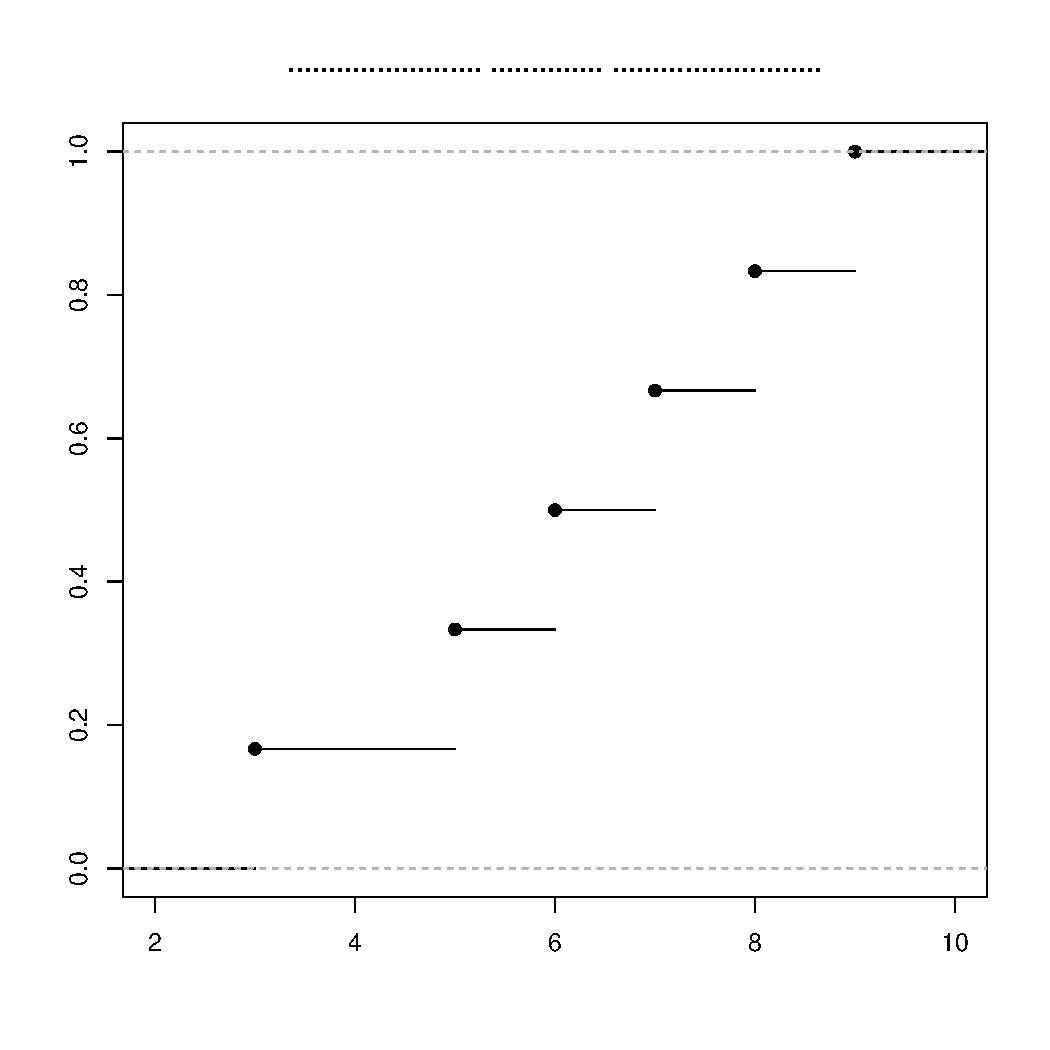
\includegraphics[width=\maxwidth]{figure/logis_pdf-1} 


\begin{figure}
\begin{tikzpicture}[scale = 0.025]
  % Created by tikzDevice version 0.10.1 on 2017-08-29 12:28:48
% !TEX encoding = UTF-8 Unicode
\definecolor{fillColor}{RGB}{255,255,255}
\path[use as bounding box,fill=fillColor,fill opacity=0.00] (0,0) rectangle (505.89,505.89);
\begin{scope}
\path[clip] (  0.00,  0.00) rectangle (505.89,505.89);
\definecolor{drawColor}{RGB}{0,0,0}

\path[draw=drawColor,line width= 0.4pt,line join=round,line cap=round] ( 74.47, 73.44) -- (460.22, 73.44);

\path[draw=drawColor,line width= 0.4pt,line join=round,line cap=round] ( 74.47, 73.44) -- ( 74.47, 66.24);

\path[draw=drawColor,line width= 0.4pt,line join=round,line cap=round] (170.91, 73.44) -- (170.91, 66.24);

\path[draw=drawColor,line width= 0.4pt,line join=round,line cap=round] (267.34, 73.44) -- (267.34, 66.24);

\path[draw=drawColor,line width= 0.4pt,line join=round,line cap=round] (363.78, 73.44) -- (363.78, 66.24);

\path[draw=drawColor,line width= 0.4pt,line join=round,line cap=round] (460.22, 73.44) -- (460.22, 66.24);

\node[text=drawColor,anchor=base,inner sep=0pt, outer sep=0pt, scale=  1.00] at ( 74.47, 47.52) {2};

\node[text=drawColor,anchor=base,inner sep=0pt, outer sep=0pt, scale=  1.00] at (170.91, 47.52) {4};

\node[text=drawColor,anchor=base,inner sep=0pt, outer sep=0pt, scale=  1.00] at (267.34, 47.52) {6};

\node[text=drawColor,anchor=base,inner sep=0pt, outer sep=0pt, scale=  1.00] at (363.78, 47.52) {8};

\node[text=drawColor,anchor=base,inner sep=0pt, outer sep=0pt, scale=  1.00] at (460.22, 47.52) {10};

\path[draw=drawColor,line width= 0.4pt,line join=round,line cap=round] ( 59.04, 87.27) -- ( 59.04,433.02);

\path[draw=drawColor,line width= 0.4pt,line join=round,line cap=round] ( 59.04, 87.27) -- ( 51.84, 87.27);

\path[draw=drawColor,line width= 0.4pt,line join=round,line cap=round] ( 59.04,156.42) -- ( 51.84,156.42);

\path[draw=drawColor,line width= 0.4pt,line join=round,line cap=round] ( 59.04,225.57) -- ( 51.84,225.57);

\path[draw=drawColor,line width= 0.4pt,line join=round,line cap=round] ( 59.04,294.72) -- ( 51.84,294.72);

\path[draw=drawColor,line width= 0.4pt,line join=round,line cap=round] ( 59.04,363.87) -- ( 51.84,363.87);

\path[draw=drawColor,line width= 0.4pt,line join=round,line cap=round] ( 59.04,433.02) -- ( 51.84,433.02);

\node[text=drawColor,rotate= 90.00,anchor=base,inner sep=0pt, outer sep=0pt, scale=  1.00] at ( 41.76, 87.27) {0.0};

\node[text=drawColor,rotate= 90.00,anchor=base,inner sep=0pt, outer sep=0pt, scale=  1.00] at ( 41.76,156.42) {0.2};

\node[text=drawColor,rotate= 90.00,anchor=base,inner sep=0pt, outer sep=0pt, scale=  1.00] at ( 41.76,225.57) {0.4};

\node[text=drawColor,rotate= 90.00,anchor=base,inner sep=0pt, outer sep=0pt, scale=  1.00] at ( 41.76,294.72) {0.6};

\node[text=drawColor,rotate= 90.00,anchor=base,inner sep=0pt, outer sep=0pt, scale=  1.00] at ( 41.76,363.87) {0.8};

\node[text=drawColor,rotate= 90.00,anchor=base,inner sep=0pt, outer sep=0pt, scale=  1.00] at ( 41.76,433.02) {1.0};

\path[draw=drawColor,line width= 0.4pt,line join=round,line cap=round] ( 59.04, 73.44) --
	(475.65, 73.44) --
	(475.65,446.85) --
	( 59.04,446.85) --
	( 59.04, 73.44);
\end{scope}
\begin{scope}
\path[clip] (  0.00,  0.00) rectangle (505.89,505.89);
\definecolor{drawColor}{RGB}{0,0,0}

\node[text=drawColor,anchor=base,inner sep=0pt, outer sep=0pt, scale=  1.20] at (267.35,471.40) {\bfseries Эмпирическая функция распределения};
\end{scope}
\begin{scope}
\path[clip] ( 59.04, 73.44) rectangle (475.65,446.85);
\definecolor{drawColor}{RGB}{0,0,0}

\path[draw=drawColor,line width= 0.4pt,line join=round,line cap=round] ( 26.25, 87.27) -- (122.69, 87.27);

\path[draw=drawColor,line width= 0.4pt,line join=round,line cap=round] (122.69,144.90) -- (219.13,144.90);

\path[draw=drawColor,line width= 0.4pt,line join=round,line cap=round] (219.13,202.52) -- (267.34,202.52);

\path[draw=drawColor,line width= 0.4pt,line join=round,line cap=round] (267.34,260.14) -- (315.56,260.14);

\path[draw=drawColor,line width= 0.4pt,line join=round,line cap=round] (315.56,317.77) -- (363.78,317.77);

\path[draw=drawColor,line width= 0.4pt,line join=round,line cap=round] (363.78,375.40) -- (412.00,375.40);

\path[draw=drawColor,line width= 0.4pt,line join=round,line cap=round] (412.00,433.02) -- (505.89,433.02);
\definecolor{fillColor}{RGB}{0,0,0}

\path[draw=drawColor,line width= 0.4pt,line join=round,line cap=round,fill=fillColor] (122.69,144.90) circle (  2.70);

\path[draw=drawColor,line width= 0.4pt,line join=round,line cap=round,fill=fillColor] (219.13,202.52) circle (  2.70);

\path[draw=drawColor,line width= 0.4pt,line join=round,line cap=round,fill=fillColor] (267.34,260.14) circle (  2.70);

\path[draw=drawColor,line width= 0.4pt,line join=round,line cap=round,fill=fillColor] (315.56,317.77) circle (  2.70);

\path[draw=drawColor,line width= 0.4pt,line join=round,line cap=round,fill=fillColor] (363.78,375.40) circle (  2.70);

\path[draw=drawColor,line width= 0.4pt,line join=round,line cap=round,fill=fillColor] (412.00,433.02) circle (  2.70);
\definecolor{drawColor}{gray}{0.70}

\path[draw=drawColor,line width= 0.4pt,dash pattern=on 4pt off 4pt ,line join=round,line cap=round] ( 59.04, 87.27) -- (475.65, 87.27);

\path[draw=drawColor,line width= 0.4pt,dash pattern=on 4pt off 4pt ,line join=round,line cap=round] ( 59.04,433.02) -- (475.65,433.02);
\end{scope}

\end{tikzpicture}
\end{figure}



\end{enumerate}


\subsubsection*{Часть 2}

\begin{flushright}
 — Это невозможно! \\
— Нет. Это необходимо.\\
\textcopyright \hspace{0.1cm} Interstellar
\end{flushright}

\begin{enumerate}
\item
Алгоритм решения: рисуешь дерево $\rightarrow$ PROFIT

\begin{center}

 \begin{tikzpicture}[->,>=stealth',shorten >=1pt,auto,node distance=3cm,
  thick,main node/.style={circle,fill=blue!20,draw,font=\sffamily\Large\bfseries}]

  \node[main node] (1) {1};
  \node[main node] (2) [below of=1] {2};
  \node[main node] (3) [below of=2] {3};

  \path[every node/.style={font=\sffamily\small}]
    (1) edge [loop right] node {«не 6»} (1)
        edge [bend right] node[left] {«6»} (2)
    (2) edge [bend right] node[right] {«не 6»} (1)
        edge [above] node[left] {«6»} (3);
\end{tikzpicture}

\end{center}

Комментарии к построению дерева: состояние 1 — начальное, состояние 3 — конец игры, когда выпало две «шестерки» подряд. Заметим, что выпадение любой «нешестерки» в процессе игры приводит нас к состоянию, эквивалентному начальному.

Вероятность выпадения «шестерки» равна 1/6, «нешестерки» — 5/6.

Теперь мы готовы оседлать коня!

\begin{enumerate}
\item $\P(N = 1) = 0$ — невозможно за ход закончить игру.

$\P(N = 2) = \frac{1}{36}$

$\P(N = 3) = \frac{5}{6} \cdot \frac{1}{6} \cdot \frac{1}{6} = \frac{5}{216}$

\item А теперь будет видна вся сила рисования дерева:

Пусть $\E_1$ — число ходов, за которое мы ожидаем закончить игру, если игра начинается в состоянии 1, $\E_2$ — число ходов, за которое мы ожидаем закончить игру, если игра начинается в состоянии 2.

Получим два уравнения:
$\begin{cases} \E_2 = \frac{1}{6} \cdot 1 +  \frac{5}{6} (\E_1 + 1)   \\ \E_1 =  \frac{5}{6} (\E_1 + 1) + \frac{1}{6} ( \E_2 + 1) \end{cases} $

Решив эту систему, получим, что $\E_1 = 42$. А ведь это и есть $\E(N)$.


Аналогична логика для оставшихся мат. ожиданий.

Найдем математическое ожидание суммы набранных очков. Ясно, что если выпадает «не 6», то мы ждем 3 очка. Тогда переопределив $\E_1$ и $\E_2$ следующим образом: пусть $\E_1$ — число набранных очков, которое мы ожидаем получить за игру, если игра начинается в состоянии 1, $\E_2$ — число набранных очков, которое мы ожидаем получить за игру, если игра начинается в состоянии 2.

Новые два уравнения:
$\begin{cases} \E_2 = \frac{1}{6} \cdot 6 +  \frac{5}{6} (\E_1 + 3)   \\ \E_1 =  \frac{5}{6} (\E_1 + 3) + \frac{1}{6} ( \E_2 + 6) \end{cases} $

Решаем и получаем: $\E(S) = \E_1 = 147$

А можно было сделать еще круче! Выше показано, что  $\E(N) = 42$. А сколько мы ждем очков за 1 ход? 3.5! Тогда $\E(S) = \E(N) \cdot 3.5 = 147$

Применяя схожую логику для $\E(N^2)$:\\
\[\E(N^2) = \frac{5}{6} \cdot \E\left((N + 1)^2\right) + \frac{1}{6} \cdot \frac{5}{6}  \cdot \E\left((N + 2)^2\right) + \frac{1}{6} \cdot \frac{1}{6} \cdot 2^2\]

Учитывая, что $\E(N) = 42$, получим: $\E(N^2) = 3414$.

\item Veni, vidi, vici
\begin{center}
  \begin{tabular}{@{}cc@{}}
  \toprule
  $X_n$       & $6$ \\ \midrule
  $\P(\cdot)$ & $1$ \\ \bottomrule
  \end{tabular}
\end{center}

\end{enumerate}

\item
\begin{enumerate}
\item $\P(V = 1) = 1/30$, т.к. именно этому равна вероятность того, что Вовочка стоит ровно вторым в очереди;

$M = 1$ значит, что между Машенькой и Вовочкой ровно один человек в очереди. Если Вовочка находится от 3 (включительно) до 28 позиции в очереди, то для Машеньки есть две благоприятные позиции для события $M = 1$ (например, если Вовочка стоит на 15 месте, то благоприятные позиции для Машеньки — стоять либо 13-ой, либо 17-ой). Если же Вовочка стоит на других позициях в очереди, то для Машеньки существует ровно одна благоприятная позиция:

\[\P(M = 1) = \frac{26}{30} \cdot \frac{2}{29} +  \frac{4}{30} \cdot \frac{1}{29} = \frac{56}{30\cdot 29} = \frac{28}{435}\]

$M = V$ произойдет только, если Машенька стоит за Вовочкой. При этом для Машеньки существует только одна благоприятная позиция и только в том случае, что Вовочка стоит до 15 позиции (включительно):
\[\P(M = V) = \frac{1}{2} \cdot \frac{1}{29} = \frac{1}{58} \]

\item \[\E(V) = \frac{0 + 1 + \ldots + 29}{30} = \frac{30\cdot 14 + 15}{30} = 14.5\]

Для $\E(M)$ можно решить в лоб, и получится красивая сумма, а можно вот так:

Сначала случайно кинем Вовочку и Машеньку на две из 30 позиций в очереди. Образуется три отрезка: точки между Вовочкой и Машенькой и два крайних отрезка (может быть, отрезок из 0 точек). Затем будем закидывать в очередь на оставшиеся позиции случайно 28 оставшихся людей (назовем их «пропавшими»). Т.к. все броски были случайны (или из соображений симметрии, как хотите), вероятность попасть в отрезок между Машенькой и Вовочкой для «пропавшего» равна $1/3$, вне отрезка — соответственно $2/3$, и независима от остальных бросков (!).

Введем случайную величину $X_i$ для $i$-го «пропавшего», которая равна $1$, если он попал в отрезок между Машенькой и Вовочкой, $0$, если не попал:


\begin{center}
\begin{tabular}{ccc}
\toprule
$X_i$ & $1$ & $0$ \\ \midrule
$\P(\cdot)$ & $1/3$ & $2/3$ \\ \bottomrule
\end{tabular}

\end{center}


Легко считается: $\E(X_i) = 1/3$, $\E(X^2_i) = 1/3$, $\Var(X_i) = 1/3 - 1/9 = 2/9$.
Ясно, что $M = \sum_1^{28} X_i$. Тогда учитывая независимость $X_i$:

\[\E(M) = \frac{28}{3}\]
\[\Var(M) = \frac{56}{9}\]
\end{enumerate}

\item
Биномиальное распределение — \textit{À l’abordage!}.

Задача интерпретируется так: последний ход — это когда мы обратились к коробку, в котором нет спичек (т.е. к одному коробку нужно обратиться $n+1$ раз).

\begin{enumerate}
\item Если $0<k \leqslant n$, будем считать успехом — попадание в коробок, к которому мы на последнем ходу игры (пустому коробку) обратились. До этого момента из негомбыло вытащено $n$ спичек, а из другого $2n-k$ спичек, т.е. всего в игре было $2n - k + 1$ шагов. Успехов — $n + 1$ (вытащено $n$ спичек, и на последнем ходу мы к нему обратились). По формуле Бернулли получаем следующее ($X$ — случайная величина, показывающая сколько спичек осталось в коробке, к которому мы не обратились на последнем ходу игры):
\[\P(X = k) = C^{n+1}_{2n-k+1} \left(\frac{1}{2} \right)^{2n-k+1}\]

Если $k = 0$, то мы вытащили все спички из обоих коробков к последнему ходу, и нам без разницы к какому коробку мы обратимся на последнем шагу, т.е.:
\[\P(X = 0) =2 C^{n+1}_{2n+1} \left(\frac{1}{2} \right)^{2n+1}\]

\item Среднее спичек в другом коробке:

\[\E(X) = \sum \limits_{k=1}^{n} k \cdot C^{n+1}_{2n-k+1} \left(\frac{1}{2} \right)^{2n-k+1}\]


\end{enumerate}


\item
Для того чтобы количество упаковок, которые необходимо купить, равнялось 50, нужно чтобы ни одну из наклеек Покупатель не встретил дважды, поэтому:
\[
\P(X=50) = 1\cdot\frac{49}{50}\cdot\frac{48}{50}\cdot\dots\cdot\frac{1}{50} = \frac{49!}{50^{49}} \approx 3.4\cdot
10^{-21}\] \vspace{-1cm}

\hspace{10.5cm}\fcolorbox{ForestGreen}{white}{Dum spiro, spero!}\footnote[2]{Надежда умирает последней!}

Теперь введем понятие «шаг». Переход на новый шаг происходит в тот момент, когда покупатель получил наклейку, которой у него раньше не было. Начинаем с шага 0, когда нет ни одной наклейки, и шагать будем до 49, потому что в момент перехода на шаг 50 Покупатель получит последнюю необходимую наклейку и «прогулка» закончится. Введем случайную величину $X_q$ равную количеству покупок в течение шага номер $q$. Тогда $X = \sum \limits_{q=0}^{49}X_q$.  Найдем математическое ожидание $X_q$:
\[
\E(X_q) = \frac{n-q}{n}\cdot 1 + \frac{q}{n}\cdot\frac{n-q}{n}\cdot 2 + \left(\frac{q}{n}\right)^2\cdot\frac{n-q}{n}\cdot 3 + \ldots
\]
здесь $\frac{n-q}{n}$ —  это вероятность найти наклейку, которой еще нет, а $\frac{q}{n}$, соответственно — вероятность повториться. Вопрос теперь в том, как посчитать сумму:
\[
\E(X_q) = \frac{n-q}{n}\left( 1 + \frac{q}{n}\cdot 2 + \left(\frac{q}{n}\right)^2 \cdot 3 + \ldots\right) = \frac{n-q}{n}\cdot\sum\limits_{k=0}^{\infty}\left(\frac{q}{n}\right)^k(k+1)
\]

Можем выписать в столбик несколько первых членов вышестоящей суммы:
\[
\begin{array}{l}
\hspace{0.3cm}1 \\
\vspace{0.2cm}
\left(\frac{q}{n}\right)^1  + \left(\frac{q}{n}\right)^1  \\
\vspace{0.2cm}
\left(\frac{q}{n}\right)^2 + \left(\frac{q}{n}\right)^2  + \left(\frac{q}{n}\right)^2 \\
\left(\frac{q}{n}\right)^3 + \left(\frac{q}{n}\right)^3 + \left(\frac{q}{n}\right)^3 + \left(\frac{q}{n}\right)^3 \\
\hspace{0.1cm}\cdots\cdots\cdots\cdots\cdots\cdots\cdots\cdots\cdots\cdots\cdots
\end{array}
\]
Достаточно! Можем скомпоновать всю сумму другим способом, а именно — по столбцам. Заметим, что сумма элементов в каждом столбце это сумма бесконечно убывающей геометрической прогрессии с одним и тем же знаменателем $\frac{q}{n}$ и различными первыми членами. Соответственно:

\[
\sum\limits_{k=0}^{\infty}\left(\frac{q}{n}\right)^k(k+1) = \frac{1}{1-\frac{q}{n}} + \frac{\frac{q}{n}}{1-\frac{q}{n}} + \frac{\left(\frac{q}{n}\right)^2}{1-\frac{q}{n}} + \frac{\left(\frac{q}{n}\right)^3}{1-\frac{q}{n}} + \dots =
\]
\[
= \frac{1}{1-\frac{q}{n}}\left( 1 + \frac{q}{n} + \left(\frac{q}{n}\right)^2 + \left(\frac{q}{n}\right)^3 + \dots\right) = \frac{n}{n-q}\cdot\frac{n}{n-q} = \left( \frac{n}{n-q}\right)^2
\]

Таким образом, получаем, что:
\[
\E(X_q) = \frac{n-q}{n}\cdot \left( \frac{n}{n-q}\right)^2 = \frac{n}{n-q}
\]
\hspace{10cm} и это верно для любого q!

\[
\E(X) = \E\left(\sum \limits_{q=0}^{49}X_q\right) = \sum \limits_{q=0}^{49}\E(X_q) =
\frac{50}{50-0} + \frac{50}{50-1} + \dots + \frac{50}{50-49} = 50\left(\frac{1}{50} + \frac{1}{49} + \dots + 1\right) \approx
\]
\[
\approx 50\int\limits_{1}^{50}\frac{1}{x}\mathbf{d}x = 50\ln(50) \approx 195.5
\]

А теперь ещё одно решение:


Величины $X_q$ независимы (но по разному распределены). Если долго пришлось ждать $i$-го шага, это ничего не говорит о $j$-ом шаге. Величины $X_q$ имеют известный закон распределения — это число опытов до первого успеха при заданной вероятности успеха. Это геометрическое распределение, математическое ожидание которого равно $\frac{1}{p}$, а дисперсия: $\frac{1-p}{p^2}$, где $p$ — \vspace{0.2cm}  вероятность успеха.

А те, кто забыл, могут \textbf{проще решить} методом первого шага:
Если $X$ — число опытов до успеха при вероятности успеха $p$, то
\[
\E(X)=p\cdot 1 + (1-p)\cdot \E(X+1)
\]
Откуда $\E(X)=\frac{1}{p}$ и дело в шляпе :)
Аналогично:
\[
\E(X^2)=p\cdot 1^2 + (1-p) \cdot \E((X+1)^2)
\]
и решая, находим $\E(X^2)$.



\item
\begin{enumerate}
\item Необходимое и достаточное условие — старушка не должна занять чужое место. С вероятностью $\frac{1}{n}$ она угадает свое место, значит, для каждого входящего его место будет свободно и он туда сядет.\\
\textbf{Ответ:} $\frac{1}{n}$
\item Будем искать вероятность того, что последний человек не сядет на свое место.

Пусть $A_i = \{\text{Старушка села на  место } i\text{-го} \}$,  $B_{(i,j)} = \{i \text{-ый  пассажир сел на место } j\text{-ого} \}$

\[
P[n\text{-ый не сядет на свое место}] = \P(A_n) + P[A_{n-1}]P[B_{(n-1,n)}]+
\]
\[
+ P[A_{n-2}](P[B_{(n-2,n)}]
+ P[B_{(n-2,n-1)}]P[B_{(n-1,n)}]  ) + \dots
\]

Можем заметить, что:
\renewcommand{\labelitemi}{$\checkmark$}
\begin{itemize}
\item $\P[A_i] = P[A_j] = \frac{1}{n}$ $\forall \hspace{0.1cm} i, j$
\item $\P[B_{(n-1,n)}]=\frac{1}{2}$, потому что $n-1$-ый выбирает из двух оставшихся мест
\item $\P[B_{(n-2,n)}]
+ \P[B_{(n-2,n-1)}]P[B_{(n-1,n)}]  = \frac{1}{3} + \frac{1}{3}\cdot \frac{1}{2} = \frac{1}{2}$
\item
\begin{multline*}
\P[B_{(n-3,n)}] + \P[B_{(n-3,n-2)}](\P[B_{(n-2,n)}]+\P[B_{(n-2,n-1)}]\P[B_{(n-1,n)}])+\\
+ \P[B_{(n-3,n-1)}]\P[B_{(n-1,n)}] =   \frac{1}{4}+\frac{1}{4}\left(\frac{1}{3}+\frac{1}{3}\cdot\frac{1}{2}\right) +\frac{1}{4}\cdot \frac{1}{2} = \frac{1}{2}
\end{multline*}
\item И так далее до того момента, пока старушка не сядет на место первого человека, который заходит после нее, — всего $n-2$ вариантов.
\end{itemize}

Таким образом мы получаем сумму:
\[
\P[n\text{-ый не сядет на свое место}] = \frac{1}{n} + \frac{1}{n}\cdot \frac{1}{2} + \frac{1}{n}\cdot \frac{1}{2} + \dots = \frac{1}{n}  + \frac{1}{2n}(n-2) = \frac{1}{2}
\]
\begin{center}
\fcolorbox{ForestGreen}{white}{
Значит вероятность $\P[n\text{-ый сядет на свое место}] = 1 -\frac{1}{2} = \frac{1}{2}$}
\end{center}

А вот ещё один вариант решения:

\underline{Метод математической индукции:} допустим что это утверждение доказано для одного, двух и так далее до $k$ человек. Рассмотрим $k+1$ человека. Когда последний сядет на своё место? Если старушка сядет на своё место, а вероятность этого равна $\frac{1}{k+1}$ или, с вероятностью $\frac{1}{2}$ (по индукции), если старушка сядет на любое место кроме своего и последнего, то есть $\frac{1}{2}\cdot\frac{k-1}{k+1}$. В этом случае тот\vspace{0.2cm} пассажир, чье место  она заняла, становится старушкой, и мы получаем задачу при меньшем $k$. Складывая эти две дроби, получаем $\frac{1}{2} $.

Чтобы найти среднее число пассажиров, разобьем эту величину в сумму индикаторов: $Y_1$ — сел ли первый на место, $\dots$, $Y_n$ — сел ли $n$-ый на место (индикатор равен единице, если сел).

Стало быть $\E(Y)=\E(Y_1)+\E(Y_2)+\ldots+\E(Y_n)$. $\E(Y_n)=\frac{1}{2}$.

Почти аналогично можем рассуждать для предпоследнего:

База индукции: если пассажиров трое ($n=3$ включая старушку), то для предпоследнего вероятность сесть на своё место равна $\frac{2}{3}$.

Шаг индукции: допустим что для $3, 4, \ldots n$ пассажиров эта вероятность равна $\frac{2}{3}$.
Рассмотрим случай $(n+1)$-го пассажира.
Предпоследний сядет на своё место, если:

\renewcommand{\labelitemi}{\textbullet}

\begin{itemize}
\item старушка сядет на своё место или на место последнего $\frac{2}{n+1}$
\item в $\frac{2}{3}$ тех случаев, когда старушка сядет на место $2, 3, \ldots, (n-1)$, т.е. $\frac{2}{3}\cdot \frac{n-2}{n+1}$
складываем, получаем $\frac{2}{3}$.
То есть по индукции вероятность того, что предпоследний сядет на своё место равна $\frac{2}{3}$
\end{itemize}
И по аналогии можно увидеть, что вероятность того, что $k$-ый с конца пассажир сядет на своё место равна $k/(k+1)$

Если у нас $n$ пассажиров включая СС, то среднее количество севших на свои места (раскладывая с конца) равно \[\frac{1}{2}+\frac{2}{3}+\frac{3}{4}+\dots+\frac{n-1}{n}+\frac{1}{n}\]

\end{enumerate}

\end{enumerate}



\subsection{Контрольная работа 2. Базовый поток. 15.12.2014}


\begin{enumerate}
\item Ежемесячные расходы студенческой семьи Маши и Васи хорошо описываются случайным
вектором $(X,Y)$, ($X$ — расходы Маши, $Y$ — расходы Васи), имеющим равномерное
распределение в треугольнике, задаваемом ограничениями $\{0 \leq X, \; 0\leq Y, \; X+Y \leq 1 \}$.

Найдите:

\begin{enumerate}
\item Вероятность того, что совокупные расходы превысят половину бюджета, $\P(X+Y>1/2)$
\item Плотность распределения расходов Васи.
\item Вероятность того, что Машины расходы составили менее трети бюджета, если
известно, что Вася израсходовал более половины семейного бюджета.
\item Условную плотность распределения и условное математическое ожидание расходов Маши, при условии, что Вася израсходовал половину бюджета.
\item Математическое ожидание условного математического ожидания расходов Маши, $\E(\E(X|Y))$
\item Коэффициент корреляции расходов Маши и Васи
\end{enumerate}

\item Задана последовательность независимых случайных величин $X_1$, $X_2$, \ldots

\begin{tabular}{llll}
\toprule
$X_n$ & $-\sqrt{n}$ & $0$ & $\sqrt{n}$ \\ \midrule
$\P(\cdot)$ & $1/2n$ & $1-1/n$ & $1/2n$ \\
\bottomrule
\end{tabular}

\begin{enumerate}
\item Сформулируйте закон больших чисел. Выполняется ли для данной последовательности
закон больших чисел?
\item Запишите неравенство Чебышёва. Оцените вероятность того, что модуль среднего
значения по $n$ наблюдениям не превысит $1$, $\P(|\bar X_n| \leq 1)$
\item Сколько членов последовательности необходимо взять, чтобы вероятность того, что
модуль среднего значения не превысит $1$, была не менее $0.9$, $\P(|\bar X_n| \leq 1)\geq 0.9$
\end{enumerate}

\item Размер выплат каждому клиенту банка — случайная величина с математическим
ожиданием, равным 5000 ед. и среднеквадратическим отклонением, равным 2000 ед.
Выплаты отдельным клиентам независимы. Сколько должно быть наличных денег в банке,
чтобы с вероятностью 0.95 денег хватило на обслуживание 60 клиентов?

\item Рекламная компания хочет оценить вероятность $p$, с которой адресная реклама приводит к
заявке. С этой целью она  рассылает $n$ рекламных проспектов. Обозначим за $\hat p$ отношение
числа поданных заявок к числу разосланных проспектов $n$. С помощью теоремы Муавра–Лапласа и неравенства Чебышёва определите:
\begin{enumerate}
\item  Сколько нужно разослать рекламных проспектов, для того чтобы $\hat p$ отличалось от
истинной вероятности $p$ не более, чем на $0.1$ с вероятностью не меньшей $0.99$
\item С какой точностью $\varepsilon$ удастся оценить $p$ с вероятностью 0.99, если разослана 1000
проспектов, т.е. $\P(|\hat p - p|\leq \varepsilon)\geq 0.99$?
\end{enumerate}
\end{enumerate}





\subsection{Контрольная работа 2. Базовый поток. 15.12.2014, решение}


\begin{enumerate}
\item
\begin{enumerate}
\item
Так как $(X, Y)$ имеют совместное равномерное распределение, $\P\left\{X+Y > \frac{1}{2}\right\}$ можно рассчитать как отношение соответствующих площадей:
\begin{center}
\definecolor{zzttqq}{rgb}{0.6,0.2,0.}
\begin{tikzpicture}[line cap=round,line join=round,>=triangle 45,x=5.692307692307692cm,y=5.692307692307692cm]
\draw[->,color=black] (-0.1,0.) -- (1.2,0.);
\foreach \x in {,0.2,0.3,0.4,0.5,0.6,0.7,0.8,0.9,1.,1.1}
\draw[shift={(\x,0)},color=black] (0pt,2pt) -- (0pt,-2pt) node[below] {\footnotesize $\x$};
\draw[->,color=black] (0.,-0.1) -- (0.,1.2);
\foreach \y in {0.2,0.3,0.4,0.5,0.6,0.7,0.8,0.9,1.,1.1}
\draw[shift={(0,\y)},color=black] (2pt,0pt) -- (-2pt,0pt) node[left] {\footnotesize $\y$};
\draw[color=black] (0pt,-10pt) node[right] {\footnotesize $0$};
\clip(-0.1,-0.1) rectangle (1.2,1.2);
\fill[color=zzttqq,fill=zzttqq,fill opacity=0.1] (0.,0.5) -- (0.5,0.) -- (1.,0.) -- (0.,1.) -- cycle;
\draw (0.,1.)-- (1.,0.);
\draw [color=zzttqq] (0.,0.5)-- (0.5,0.);
\draw [color=zzttqq] (0.5,0.)-- (1.,0.);
\draw [color=zzttqq] (1.,0.)-- (0.,1.);
\draw [color=zzttqq] (0.,1.)-- (0.,0.5);
\draw (0.344196516991,0.436512272899) node[anchor=north west] {$S_0$};
\draw (0.129676687465,0.218325437741) node[anchor=north west] {$S_1$};
\draw (0.0233335241101,1.16441289103) node[anchor=north west] {$y$};
\draw (1.06109611823,0.08) node[anchor=north west] {$x$};
\end{tikzpicture}
\end{center}

Соответственно: \[\P\left(X+Y > \frac{1}{2}\right) = \frac{S_0}{S_0+S_1} = \frac{0.5-S_1}{0.5} = \frac{\frac{1}{2}-\frac{1}{8}}{\frac{1}{2}} = \frac{3}{4}\]

\item
\[
f_Y(y) = \int \limits_{0}^{1-y} f_{XY}(x,y) dx
\]

Поэтому, нам сначала нужно найти $f_{XY}(x,y)$, которая для равномерного распределения должна быть константой. Это можно сделать из условия:
\[
\int\limits_{0}^{1}\int \limits_{0}^{1-x} f_{XY}(x, y) dxdy = \int\limits_{0}^{1}\int \limits_{0}^{1-x} C dxdy = 1 \Rightarrow
\]
\[
\int\limits_{0}^{1}\int \limits_{0}^{1-x} C dxdy = \int\limits_{0}^{1} C(1-x) dx = \left. \left( Cx-C\frac{x^2}{2}\right) \right| _{0}^{1} =
 \frac{C}{2}  = 1\]

 Откуда имеем $f_{XY}(x, y) = C = 2$. Теперь можем найти плотность распределения расходов Васи:
 \[ f_Y(y) = \int \limits_{0}^{1-y} 2 dx = 2(1-y) \]



\item В данном случае площади немного другие, но смысл тот же:

\begin{center}
\definecolor{zzttqq}{rgb}{0.6,0.2,0.}
\begin{tikzpicture}[line cap=round,line join=round,>=triangle 45,x=5.692307692307692cm,y=5.692307692307692cm]
\draw[->,color=black] (-0.1,0.) -- (1.2,0.);
\foreach \x in {,0.2,0.3,0.4,0.5,0.6,0.7,0.8,0.9,1.,1.1}
\draw[shift={(\x,0)},color=black] (0pt,2pt) -- (0pt,-2pt) node[below] {\footnotesize $\x$};
\draw[->,color=black] (0.,-0.1) -- (0.,1.2);
\foreach \y in {,0.2,0.3,0.4,0.5,0.6,0.7,0.8,0.9,1.,1.1}
\draw[shift={(0,\y)},color=black] (2pt,0pt) -- (-2pt,0pt) node[left] {\footnotesize $\y$};
\draw[color=black] (0pt,-10pt) node[right] {\footnotesize $0$};
\clip(-0.1,-0.1) rectangle (1.2,1.2);
\fill[color=zzttqq,fill=zzttqq,fill opacity=0.1] (0.,0.5) -- (0.,1.) -- (0.333333333333,0.666666666667) -- (0.333333333333,0.5) -- cycle;
\draw (0.,1.)-- (1.,0.);
\draw[dashed] (1/3, 2/3) -- (1/3,0);
\draw (0.1004007648034,0.729040237615) node[anchor=north west] {$S_0$};
\draw (0.343364031073,0.5908861537646) node[anchor=north west] {$S_1$};
\draw (0.0233335241101,1.16441289103) node[anchor=north west] {$y$};
\draw (1.06109611823,0.08) node[anchor=north west] {$x$};
\draw (0.,0.5)-- (0.5,0.5);
\draw [color=zzttqq] (0.,0.5)-- (0.,1.);
\draw [color=zzttqq] (0.,1.)-- (0.333333333333,0.666666666667);
\draw [color=zzttqq] (0.333333333333,0.666666666667)-- (0.333333333333,0.5);
\draw [color=zzttqq] (0.333333333333,0.5)-- (0.,0.5);
\end{tikzpicture}
\end{center}


\[\P\left( \left. X<\frac{1}{3} \hspace{1mm} \right| Y>\frac{1}{2}\right) = \frac{S_0}{S_0+S_1} = \frac{\frac{1}{8} - S_1}{\frac{1}{8}} = \frac{\frac{1}{8}-\frac{1}{72}}{\frac{1}{8}} = \frac{8}{9}\]

\item При $Y = \frac{1}{2}$, $X$ распределен равномерно от 0 до $\frac{1}{2}$, поэтому его плотность равна \[f_X(x) = \frac{1}{\frac{1}{2} - 0} = 2\]
Соответственно, условное математическое ожидание:
\[
\E \left( X| Y =\frac{1}{2}\right) = \frac{1}{4}
\]

\item $\E(\E(X|Y)) = \E(X)$, а маргинальную функцию плотности для $X$ мы можем найти так же, как искали для $Y$, и получим $f_X(x) = 2(1-x)$. Отсюда:
\[
\E(X) = \int \limits_{0}^{1} 2x(1-x)dx = \left .\left(x^2 - \frac{2}{3}x^3\right) \right|^{1}_{0} = \frac{1}{3}
\]

\item Если вспомнить формулу для корреляции:
\[
\rho_{XY} = \frac{\Cov(X, Y)}{\sigma_X\sigma_Y}  = \frac{\E(XY) - \E(X)\E(Y)}{\sigma_X\sigma_Y}
\]

то станет более-менее очевидно, что надо найти $\E(XY)$ и дисперсии $X$ и $Y$.

\[
\E(XY) = \int \limits_{0}^{1} \int \limits_{0}^{1-x} 2xy dxdy = \int \limits_{0}^{1} 2xdx \int \limits_{0}^{1-x}ydy =  \int \limits_{0}^{1}x(x^2-2x+1)dx =
\]
\[
= \left. \left(\frac{x^4}{4} - \frac{2}{3}x^3 + \frac{x^2}{2}\right) \right|^{1}_{0} = \frac{3}{4}-\frac{2}{3} = \frac{1}{12}
\]

Соответственно:

\[
\Cov(X, Y) = \frac{1}{12} - \frac{1}{3}\cdot \frac{1}{3} = -\frac{1}{36}
\]

Найдем теперь дисперсии $X$ и $Y$ (они будут одинаковыми, как и математические ождания, в силу симметрии):

\[
\E(X^2) = \int \limits_{0}^{1} 2x^2(1-x)dx = \left. \left( \frac{2}{3}x^2 - \frac{x_4}{2} \right) \right|_{0}^{1} = \frac{1}{6}
\]

Поэтому:
\[
\Var[X] = \E(X^2) - (\E(X))^2 = \frac{1}{6} - \frac{1}{9} = \frac{1}{18}
\]

Теперь наконец-то можем найти корреляцию:
\[
\rho_{XY} = -\frac{\frac{1}{36}}{\sqrt{\frac{1}{18}}\sqrt{\frac{1}{18}}} = -\frac{1}{2}
\]
\end{enumerate}

\item

\begin{enumerate}

\item Закон больших чисел гласит, что $\bar{X} \rightarrow
\E(X)$ при $n\rightarrow \infty$. Проверим его выполнение в данном случае:
\[
\E(X_n) = \frac{1}{2n}(-\sqrt{n}) + \left(1-\frac{1}{n}\right)\cdot0 + \frac{1}{2n}\sqrt{n} = 0
\]

\[
\lim\limits_{n\rightarrow\infty} \bar{X} = \lim\limits_{n\rightarrow\infty} \frac{X_1 +\dots + X_n}{n} = 0
\]
так как числитель ограничен, а знаменатель бесконечно возрастает.
Видим, что ЗБЧ в данном случае, конечно, выполняется.

Как вариант, можно было сказать, что дисперсия ограничена, и из этого также следует выполнение ЗБЧ.
\item Неравенство Чебышева:
\[
\P(|X-\E(X)|\geqslant \varepsilon) \leqslant \frac{\Var(X)}{\varepsilon^2}
\]

Соответственно, искомую вероятность можем оценить следующим образом:
\[
\P(|\bar{X}| \leqslant 1) = 1 -\P(|\bar{X}| \geqslant 1) \Rightarrow \P(|\bar{X}| \leqslant 1) \geqslant 1 - \frac{\Var[\bar{X}]}{1}
\]
\[
\Var[\bar{X}] = \Var\left(\frac{\sum\limits_{i=1}^{n} X_i}{n}\right) = \frac{1}{n^2}\sum \limits_{i=1}^{n} \Var{X_i}
\]
В свою очередь:

\[
\E(X_i^2) = 2\cdot\frac{1}{2n}\cdot n + \left(1-\frac{1}{n}\right)\cdot0 = 1 \Rightarrow \Var[X_i] = 1 \Rightarrow \Var[\bar{X}] = \frac{1}{n}
\]

Поэтому:
\[
\P(|\bar{X}| \leqslant 1)\geqslant 1 - \frac{1}{n}
\]

\item  \[1 - \frac{1}{n} = 0.9  \Rightarrow n = 10\]

\end{enumerate}

\item

Обозначим за $R$ — необходимое количество наличных денег в банке. Пусть $X$ — случайная величина, показывающее размер суммарной выплаты $60$ ($n$ — достаточное большое для применения ЦПТ) клиентам. Ясно, что т.к. выплаты отдельным клиентам независимы: \( \E X = 60 \cdot 5000 = 3\cdot 10^5 \); \( \Var X = 60 \cdot 2000^2 = 2.4 \cdot 10^8 \); \( \sigma_X = \sqrt{2.4} \cdot 10^4 \approx 1.55 \cdot 10^4\)

Теперь по ЦПТ:
\[\P(R \geqslant X) = 0.95 \]
\[\P \left(\frac{X - \E X}{\sigma_X} \leqslant \frac{R - \E X}{\sigma_X} \right) = 0.95 \]
\[ \P \left( Z \leqslant \frac{R - 3 \cdot 10^5}{1.55 \cdot 10^4} \right) = 0.95 \]
Слева функция распределения; подставляя 95-\% квантиль стандартного нормального распределения, получаем:
\[ \frac{R - 3 \cdot 10^5}{1.55 \cdot 10^4} = 1.64 \]
\[ R = 325420 \]


\item

\begin{enumerate}
\item По предельной теореме Муавра-Лапласа:
\[ \frac{\hat{p} - p}{\sqrt{p(1-p)/n}} \sim N (0,1) \]
\[ \P \left( \frac{|\hat{p} - p|}{\sqrt{p(1-p)/n}} \leqslant \frac{0.1}{\sqrt{p(1-p)/n}} \right) \geqslant 0.99 \]
\[ \P \left( |Z| \leqslant \frac{0.1}{\sqrt{p(1-p)/n}} \right) \geqslant 0.99 \]
Из симметричности стандартного нормального распределения и зная его 99.5-\% квантиль, равный приблизительно 2.58, получаем:
\[ \frac{0.1}{\sqrt{p(1-p)/n}} \geqslant 2.58 \]
\[ \frac{\sqrt{n}}{\sqrt{p(1-p)}} \geqslant \frac{2.58}{0.1} \]
\[ \sqrt{n} \geqslant \frac{2.58}{0.1} \sqrt{p(1-p)} \]
\[ n \geqslant 665.64 \cdot p(1-p) \]

С помощью неравенства Чебышева:
\[ \P \left( |\hat{p} - p| \leqslant 0.1 \right) \geqslant 0.99 \]
\[ \P \left( |\hat{p} - p| \geqslant 0.1 \right) \leqslant 0.01 \]
Теперь просто смотрим на неравенство Чебышева и на строчку выше, на неравенство Чебышева и на строчку выше\ldots
\[ \frac{p(1-p)/n}{0.1^2} = 0.01\]
\[ n = 10^4 p(1-p) \]
Принимаются оба ответа!

\item По предельной теореме Муавра-Лапласа:
\[ \P \left( \frac{|\hat{p} - p|}{\sqrt{p(1-p)/n}} \leqslant \frac{\varepsilon}{\sqrt{p(1-p)/1000}} \right) \geqslant 0.99 \]
\[ \P \left( |Z| \leqslant \frac{\varepsilon}{\sqrt{p(1-p)/1000}} \right) \geqslant 0.99 \]
Аналогично пункту 1:
\[ \frac{\varepsilon}{\sqrt{p(1-p)/1000}} \geqslant 2.58 \]
\[ \varepsilon \geqslant 0.082 \sqrt{p(1-p)} \]

С помощью неравенства Чебышева:
\[ \P \left( |\hat{p} - p| \leqslant \varepsilon \right) \geqslant 0.99 \]
\[ \P \left( |\hat{p} - p| \geqslant \varepsilon \right) \leqslant 0.01 \]
Аналогично пункту 1:
\[ \frac{p(1-p)/1000}{\varepsilon^2} = 0.01\]
\[ \varepsilon^2 = \frac{p(1-p)}{10} \]
\[ \varepsilon = \sqrt{\frac{p(1-p)}{10}} \approx 0.316 \sqrt{p(1-p)} \]

\end{enumerate}

Нужно было показать, как мастерство владения теоремой Муавра-Лапласа, так и неравенством Чебышева.


\end{enumerate}


\subsection{Праздник номер 2, i-поток, 15.12.2014}

Time: 180 min

\begin{enumerate}
\item Вася может получить за экзамен равновероятно либо $8$ баллов, либо $7$ баллов. Петя может получить за экзамен либо $8$ баллов — с вероятностью $1/3$; либо $7$ баллов — с вероятностью $2/3$. Известно, что корреляция их результатов равна $0.7$.

Какова вероятность того, что Петя и Вася покажут одинаковый результат?

\item В  городе Туме проводят демографическое исследование семейных пар. Стандартное отклонение возраста мужа оказалось равным 5 годам, а стандартное отклонение возраста жены — 4 годам. Найдите корреляцию возраста жены и возраста мужа, если стандартное отклонение разности возрастов оказалось равным 2 годам. В каких пределах лежит вероятность того, что возраст случайно выбираемого женатого мужчины отклоняется от своего математического ожидания больше чем на 10 лет?


\item На окружности единичной длины случайным образом равномерно и независимо друг от друга выбирают две дуги: длины $0.3$ и длины $0.4$.
\begin{enumerate}
\item  Найдите функцию распределения длины пересечения этих отрезков
\item Найдите среднюю длину пересечения
\end{enumerate}


\item  Совместная функция плотности величин $X$ и $Y$ имеет вид
\begin{equation}
\nonumber
f(x,y)=\begin{cases}
2(x^3+y^3), \text{ если } x\in [0;1], y\in [0;1] \\
0, \mbox{ иначе}
\end{cases}
\end{equation}
\begin{enumerate}
\item Найдите $\P(X+Y>1)$
\item Найдите $\Cov(X,Y)$
\item Являются ли величины $X$ и $Y$ независимыми?
\item Являются ли величины $X$ и $Y$ одинаково распределенными?
\end{enumerate}



\item Изначально цена акций компании «Пумперникель» равна $X_0=1000$ рублей. Каждый последующий день в течение 100 дней цена равновероятно может вырасти на 2 рубля или упасть на 1 рубль. Обозначим цену акции через $n$ дней как $X_n$.
\begin{enumerate}
\item Чему равны математическое ожидание и дисперсия изменения цены за отдельный день?
\item Найдите $\E(X_n)$, $\Var(X_n)$, $\Cov(X_n, X_k)$
\item Сформулируйте центральную предельную теорему
\item Примерно найдите вероятность $\P(X_{100}>1060)$
\item Биржевой игрок Вениамин утверждает, что через 100 дней с вероятностью 95\% цена акций «Пумперникель» не опустится ниже $a$. Чему равно $a$?
\end{enumerate}
\item  Сэр Фрэнсис Гальтон —  учёный XIX-XX веков, один из основоположников как
генетики, так и статистики — изучал, среди всего прочего, связь между ростом детей и родителей.  Он исследовал данные о росте 928 индивидов. Обозначим $X_1$ — рост случайного человека, а $X_2$ — среднее арифметическое роста его отца и матери. По результатам исследования Гальтона:


\[
\begin{pmatrix}
X_1 \\
X_2
\end{pmatrix}
\sim
\cN\left[
\begin{pmatrix}
68.1 \\
68.3
\end{pmatrix};
\begin{pmatrix}
6.3 & 2.1 \\
2.1 & 3.2
\end{pmatrix}
\right]
\]

\begin{enumerate}
\item Обратите внимание на то, что дисперсия роста детей выше дисперсии среднего роста
родителей. С чем это
может быть связано? Учтите, что рост детей измерялся уже по достижении
зрелости, так что разброс не должен быть связан с возрастными различиями.
\item Рассчитайте корреляцию между $X_1$ и $X_2$
\item Один дюйм примерно равен $2.54$ сантиметра. Пусть $X_1'$ и $X_2'$ — это те же $X_1$ и $X_2$, только измеренные в сантиметрах. Найдите вектор математических ожиданий и ковариационную матрицу вектора $X'=(X_1', X_2')$.
\item Определите, каков ожидаемый рост и дисперсия роста человека, средний рост родителей которого составляет 72 дюйма?
\item Найдите вероятность того, что рост человека превысит 68 дюймов, если средний рост его родителей равен 72 дюймам. Подсказка: используйте предыдущий пункт и нормальность распределения!
\end{enumerate}

%\item Пуассоновское казино. В пуассоновском казино сигнальная лампочка загорается согласно пуассоновскому потоку в среднем один раз в минуту. В любой момент азартный игрок Вениамин может нажать кнопку. Нажать кнопку Вениамин может только один раз. Вениамин срывает джек-пот,

\item Звонки поступают в пожарную часть согласно пуассоновскому потоку в среднем $2$~раза в час. Предположим, что после получения звонка пожарная часть занята тушением пожара случайное время равномерно распределённое от получаса до часа. В это время звонки перенаправляются в соседнюю пожарную часть.

Пожарная часть только-только начала работать и готова принимать звонки.
\begin{enumerate}
\item Какова вероятность того, что за ближайший час не поступит звонков?
\item Какова вероятность того, что за ближайший час не будет перенаправленных звонков?
\item Найдите закон распределения количества звонков до первого перенаправленного звонка.
\end{enumerate}

\item  Судьба Дон-Жуана


У Дон-Жуана $n$  знакомых девушек, и их всех зовут по-разному. Он пишет
им $n$  писем, но по рассеянности раскладывает их в конверты
наугад. Случайная величина $X$ обозначает количество девушек, получивших письма, адресованные лично им.

\begin{enumerate}
\item Найдите $\E(X)$, $\Var(X)$
\item Какова при большом $n$ вероятность того, что хотя бы одна девушка получит письмо, адресованное ей?
\end{enumerate}

\item Игла Бюффона

Плоскость разлинована параллельными линиями через каждый сантиметр. Случайным образом на эту плоскость бросается иголка длины $a<1$.

\begin{enumerate}
\item Какова вероятность того, что иголка пересечёт какую-нибудь линию?
\item Предложите вероятностный способ оценки числа $\pi$
\end{enumerate}


\end{enumerate}


\subsection{Решение. Праздник номер 2, i-поток}

\begin{enumerate}
\item
Пусть $X$ — оценка Пети, $Y$ — оценка Васи. Тогда исходя из условия:
\begin{center}

\begin{tabular}{ccc}
\toprule
$X$ & $7$ & $8$ \\ \midrule
$\P(\cdot)$ & $\frac{1}{2}$ & $\frac{1}{2}$ \\ \bottomrule
\end{tabular}
\hspace{1cm}
\begin{tabular}{ccc}
\toprule
$Y$ & $7$ & $8$ \\ \midrule
$\P(\cdot)$ & $\frac{2}{3}$ & $\frac{1}{3}$  \\ \bottomrule
\end{tabular}
\end{center}

Теперь можем найти математические ожидания и дисперсии:
\[
\E(X) = \frac{15}{2}, \hspace{0.5cm} \E(Y) = \frac{22}{3} \Rightarrow
\]
\[
\Var[X] = \frac{1}{2}\cdot 64 + \frac{1}{2}\cdot 49 - \left(\frac{15}{2}\right)^2 = \frac{1}{4}
\]
\[
\Var[Y] = \frac{1}{3}\cdot 64 + \frac{2}{3}\cdot 49 - \left(\frac{22}{3}\right)^2 = \frac{2}{9}
\]

Теперь из формулы для корреляции мы можем найти $\E(XY)$:

\[
0.7 = \frac{\E(XY)-\frac{15}{2}\cdot\frac{22}{3}}{\sqrt{\frac{1}{4}}\sqrt{\frac{2}{9}}} \Rightarrow \E(XY) \approx 55.16499
\]

Можем составить табличку для совместного распределения, немножко подумав:

\begin{center}
\begin{tabular}{@{}lccr@{}}
\toprule
$Y$ \textbackslash $X$ & $7$             & $8$             & $\sum$        \\ \midrule
$7$                              & $p$             & $\frac{1}{2}-p$ & $\frac{1}{2}$ \\
$8$                              & $\frac{2}{3}-p$ & $p-\frac{1}{6}$ & $\frac{1}{2}$ \\
$\sum$                           & $\frac{2}{3}$   & $\frac{1}{3}$   &               \\ \bottomrule
\end{tabular}
\end{center}

\[
\E(XY) = 49p+56\left(\frac{1}{2} - p + \frac{2}{3}-p\right) + 64\left(p-\frac{1}{6}\right) = 55.16499
\]

\[
\Rightarrow p \approx 0.4983233 \Rightarrow \P(X=Y) = p + p-\frac{1}{6} = 0.8299799
\]



\item

Пусть $M$ — возраст мужа, $F$ — возраст жены. Тогда из условия:
\[
\Var(M-F) = \Var(M) + \Var(F) - 2\Cov(M, F) = 4 \Rightarrow \Cov(M, F) = \frac{37}{2}
\]

\[
\rho_{MF} = \frac{\frac{37}{2}}{5\cdot4} = \frac{37}{40}
\]


Согласно неравенству Чебышева:
\[
\P(|M-\E(M)|\geqslant10) \leqslant\frac{\Var(M)}{10^2} = 0.25
\]

Поэтому данная вероятность лежит в пределах $(0, 25]$.

\renewcommand{\labelenumii}{(\alph{enumii})}
\item
\begin{enumerate}
\item Пусть $X$ — длина пересечения. Требуется найти $\P(X\leqslant x)$. Рассмотрим расположение центров отрезков относительно друг друга:

\begin{center}
\definecolor{zzttqq}{rgb}{0.6,0.2,0.}
\begin{tikzpicture}[line cap=round,line join=round,>=triangle 45,x=7cm,y=7]
\draw[color=black] (0.,0.) -- (1.1,0.);
\foreach \x in {0,0.5,0.3,1.1}
\draw[shift={(\x,0)},color=black, line width= 1pt] (0pt,2pt) -- (0pt,-2pt) node[below] {};
\draw (0.25,0.) node[circle, inner sep = 1pt,  fill] {};
\draw (0.7,0.) node[circle, inner sep = 1pt,  fill] {};
\draw[<->, color = black] (0,-2) -- (0.25, -2) ;
\draw[<->, color = black] (0.25,-2) -- (0.7, -2) ;
\draw[<->, color = black] (0.7,-2) -- (1.1, -2) ;
\draw[color=black, dashed] (0,0) -- (0,-2);
\draw[color=black, dashed] (0.25,0) -- (0.25,-2);
\draw[color=black, dashed] (0.7,0) -- (0.7,-2);
\draw[color=black, dashed] (1.1,0) -- (1.1,-2);
\draw (0.125,-2) node[below] {0.15};
\draw (0.4,-2) node[below] {$R$};
\draw (0.8,-2) node[below] {0.2};
\draw[color = red, line width = 2pt] (0.3, 0) -- (0.5, 0);

\end{tikzpicture}
\end{center}

Заматим, что $X = 0.15-(R-0.2) = 0.35-R$. Однако, $R \sim U\left[0, \frac{1}{2}\right]$. Можно представить, что эти точки бросают на окружность по очереди, тогда расстояние между ними не может превышать $\frac{1}{2}$ и распределено равномерно. Имеем:
\[
\P(X \leqslant x) = \P(0.35-R\leqslant x) = \P(R \geqslant 0.35-x) = \frac{0.5-0.35+x}{0.5} = 0.3+2x
\]

Строго говоря, длина пересечения не может быть больше 0.3 по понятным причинам, поэтому функция распределения выглядит так:
\[
F(x) = \begin{cases}
0.3+2x, & x < 0.3\\
1, & x \geqslant 0.3
\end{cases}
\]

\item Зная функцию распределения, можем найти плотность:
\[f_X(x) = \begin{cases}
2, & x < 3\\
0, & \text{else}
\end{cases}\]

Сответственно:
\[
\E(X) = \int \limits_{0}^{0.3} 2x dx = \left.  x^2 \right|_{0}^{0.3} = 0.09
\]
\end{enumerate}



\item

\begin{enumerate}
\item \[\P(X+Y > 1) = \iint \limits_{\mathcal{G}}2(x^3+y^3)dxdy = \int \limits_{0}^{1} dx \int \limits_{1-x}^{1}2(x^3+y^3)dy = \ldots  = 0.8\]
\item Для того, чтобы найти ковариацию, придется найти :
\[\E(X) = \int\limits_{0}^{1} dx \int\limits _{0}^{1}2x(x^3+y^3)dy = \ldots = 0.65\]
\[\E(Y) = \int\limits_{0}^{1} dy \int\limits_{0}^{1}2y(x^3+y^3)dx = \ldots = 0.65 \]
\[\E(XY) = \int\limits_{0}^{1}dx\int\limits_{0}^{1}2xy(x^3+y^3)dy = \ldots = 0.4\]

Ну а потом все просто: $\Cov(X, Y) = \E(XY) - \E(X)\E(Y) = -0.0225$

\item Проверить свойство функций плотности $f_XY(x, y) = f_X(x)\cdot f_Y(y)$, а если $\Cov(X, Y) \ne 0$, то сразу зависимы. Здесь — зависимы.
\item Да, являются.
\end{enumerate}


\item
Для этой задачи аккуратно нужно писать \( \left(\Delta X \right)_j \), но так как приращения цен независимы (см. биномиальная модель рынка в интернетах) будем писать \( \Delta X \).
\begin{enumerate}
\item \[\E (\Delta X) = 2 \cdot \frac{1}{2} - 1 \cdot \frac{1}{2} = \frac{1}{2} \]
\[\E (\Delta X)^2 = 4 \cdot \frac{1}{2} + 1 \cdot \frac{1}{2} = \frac{5}{2} \]
\[\Var (\Delta X) = \frac{5}{2} - \left(\frac{1}{2}\right)^2 = \frac{10-1}{4}=\frac{9}{4} \]
\item \[\E (X_n) = \E \left(1000 + n\Delta X \right)  = 1000 + n \E \Delta X = 1000 + 0.5 n     \]
\[ \Var (X_n) = n \Var (\Delta X) = n \frac{9}{4}  \]
\[ \Cov (X_n, X_k) = \Cov \left(X_k, X_k + (n-k) \Delta X \right)     \]
Так как цена в момент $k$ никак не связана с последующими случайными блужданиями, то:
\[ \Cov (X_n, X_k) = \Cov \left(X_k, X_k + (n-k) \Delta X \right) =  \Cov \left(X_k, X_k \right) + 0 = \Var X_k = k \frac{9}{4}    \]
\item Заметим, что для самих цен акций ЦПТ мы формулировать не можем ввиду того, что случайные величины коррелированы, не i.i.d. Зато мы можем сформулировать ее для независимых приращений!

\( \left(\Delta X \right)_1, \ldots, \left(\Delta X \right)_{k} \) — последовательность i.i.d. случайных величин (при большом $k$) с конечными математическим ожиданием \(1/2 \) и стандартным отклонением \(3/2 \). Пусть также \( S_k = \sum_{i=1}^k \left(\Delta X \right)_j \). Тогда формулировка ЦПТ:
\[ \frac{S_k - k/2}{3/2 \sqrt{k}} \sim \cN(0,1)    \]
\item Воспользуемся результатом ЦПТ!
\[\P(X_{100} > 1060) = \P (1000 + S_{100} > 1060) = \P(S_{100} >60) = \]
\[ = \P \left(\frac{S_{100} -50 }{3/2\cdot 10} > \frac{60-50}{3/2 \cdot 10}\right) = \P \left(Z > \frac{2}{3}\right) = 1-pnorm(2/3) \approx 0.25   \]

\item \[ \P \left(1000 + S_{100} > a \right) = 0.95              \]
\[ \P \left( S_{100} < a-1000 \right) = 0.05              \]
Используя ЦПТ:
\[ a-1000 = qnorm(0.05, mean = 50, sd = 15 )            \]
\[ a \approx 1025.33   \]
\end{enumerate}

\item
\[\begin{pmatrix}
X_1 \\
X_2
\end{pmatrix} \sim \cN \left( \begin{pmatrix}
68.1 \\
68.3
\end{pmatrix} ; \begin{pmatrix}
6.3 & 2.1 \\
2.1 & 3.2
\end{pmatrix}                   \right)\]

\begin{enumerate}
\item \href{http://johnhawks.net/explainer/stats/heritability-and-stature/}{Смотреть здесь}
\item \[ \Corr(X_1, X_2) = \frac{\Cov(X_1, X_2)}{\sigma_{X_1} \sigma_{X_2}} = \frac{2.1}{\sqrt{6.3\cdot 3.2}} \approx 0.47   \]
\item \[\begin{pmatrix}
X_1' \\
X_2'
\end{pmatrix} \sim \cN \left( \begin{pmatrix}
68.1\cdot 2.54 \\
68.3\cdot 2.54
\end{pmatrix} ; \begin{pmatrix}
6.3\cdot 2.54^2 & 2.1 \cdot 2.54^2\\
2.1\cdot 2.54^2 & 3.2 \cdot 2.54^2
\end{pmatrix} \right) \]
\[\begin{pmatrix}
X_1' \\
X_2'
\end{pmatrix} \sim \cN \left( \begin{pmatrix}
172.97 \\
173.48
\end{pmatrix} ; \begin{pmatrix}
40.65 & 13.55\\
13.55 & 20.61
\end{pmatrix} \right) \]
\item Универсальный способ:

Всегда можно представить $X_1$ и $X_2$ в следующем виде (из соображений ЛНЗ для $X_1$ две стандартные нормальные независимые $Z_1$ и $Z_2$):
\[X_1 = \E X_1 + a Z_1 + b Z_2 \]
\[X_2 = \E X_2 + c Z_1 \]
\[X_1 = 68.1 + a Z_1 + b Z_2 \]
\[X_2 = 68.3 + c Z_1 \]
Зная ковариационную матрицу, легко найти коэффициенты $a$, $b$, $c$:
\[\Var X_1 = a^2 + b^2 = 6.3   \]
\[\Var X_2 = c^2 = 3.2   \]
\[\Cov (X_1, X_2) = ac\Var Z_1= ac = 2.1   \]
Получаем $c = 1.79$, $a = 1.17$, $b=2.22$.
Итак: \[X_1 = 68.1 + 1.17 Z_1 + 2.22 Z_2 \]
\[X_2 = 68.3 + 1.79 Z_1 \]
Теперь легко получаем:
\begin{multline*}
\E (X_1 | X_2 = 72) = \E ( 68.1 + 1.17 Z_1 + 2.22 Z_2|  68.3 + 1.79 Z_1 = 72) =   \\
 =   \E ( 68.1 + 1.17 Z_1 + 2.22 Z_2|  Z_1 = 2.07) = \\
 = \E (68.1 + 1.17 \cdot 2.07 + 2.22 Z_2) = 70.52
\end{multline*}
Это кстати отражает довольно известный факт, что дети высоких родителей будут тоже высокими, но менее высокими: некий mean reversion (regression to the mean — узнаете в эконометрике).
\[ \Var (X_1 | X_2 = 72) = \Var ( 68.1 + 1.17 \cdot 2.07 + 2.22 Z_2) = 2.22^2 = 4.93   \]

\item Используем стандартизацию и факт о том, что условное распределение нормальных — нормальное:
\begin{multline*}
\P (X_1 > 68 | X_2 = 72)  = \P \left(\frac{(X_1 | X_2 = 72) - \E (X_1 | X_2 = 72)}{\sqrt{\Var (X_1 | X_2 = 72)}} > \frac{68 - 70.52}{\sqrt{4.93}} \right) = \\
= \P (Z> -1.135 ) = 1 - pnorm(-1.135) =0.87
\end{multline*}
\end{enumerate}

\item
\begin{enumerate}
\item \[X \sim Poiss(\lambda = 2 )\]
Тогда: \[\P (X = 0) = e^{-\lambda}= e^{-2}\approx 0.135  \]
\item Учитывая закон распределения времени на тушение пожара $Z \sim U[1/2,1]$ можно однозначно сказать, что за ближайший час может не быть перенаправленных звонков только при $X\leqslant 2$. Пусть $Y_1$ — время между 1-ым и 2-ым звонком. Оно имеет экспоненциальное распределение $Y \sim exp(1/2)$. Итак, искомая вероятность:
\[ \P (\cdot) = \P(X=0) + \P(X=1) + \P(X=2) \P(Y_1 > Z_1) \]
Сложность в нахождении вероятности $\P(Y_1 > Z_1)$. Предоставим путь в лоб:

Совместная функция плотности случайных величин $Y_1$ и $Z_1$, очевидно:
\[ p(y,z) = p(y) p(z) = 2e^{-2y} \cdot 2 = 4e^{-2y} \]
Тогда:
\begin{multline*}
\P(Y_1 > Z_1) = \int \limits_{1/2}^1 \int \limits_z^\infty 4e^{-2y}  dy dz = -\int \limits_{1/2}^1 2e^{-2y} |_z^\infty dz = \int \limits_{1/2}^1 2e^{-2z} dz= \\
= -e^{-2z} |_{1/2}^1 =e^{-1} - e^{-2}
\end{multline*}
Можно и без двойных интегралов, но более мозгоемко. Благодаря memoryless property пуассоновского потока:
\[\P(Y_1 > Z_1) = F_{Y_1} (1) - F_{Y_1} (1/2) = 1 - e^{-2} - (1 - e^{-1}) = e^{-1} - e^{-2} \]
Итак:
\[ \P (\cdot) = e^{-2} + 2 e^{-2} + 2 e^{-2} \left( e^{-1} - e^{-2} \right) \approx 0.47 \]

\item Благодаря memoryless property, вероятность перенаправления для каждого звонка, начиная со 2, равна $e^{-1} - e^{-2}$. Обозначим за $Q$ — количество звонков до первого перенаправленного звонка. \[Q - 1 \sim Geom (e^{-1} - e^{-2}) \]
\end{enumerate}



\item
\begin{enumerate}
\item Обозначим:
$X_i =
\begin{cases}
1, &\text{если i-ая девушка получила свое письмо} \\
0, &\text{иначе}
\end{cases}
$

Так как письма раскладывались рандомно, то: $\P (X_i = 1) = 1/n$. Тогда:
\[ \E X_i = \frac{1}{n} \]
\[ \E X_i^2 = \frac{1}{n} \]
\[ \Var X_i = \frac{1}{n} - \frac{1}{n^2} \]

Легко найти:
\[ \E X = \E (X_1 + \ldots + X_n) = n \E X_i = 1 \]

Для поиска дисперсии понадобятся ковариации, так как ясно, что если одна из девушек получила свое письмо, значит, она не отняла чье-то письмо, а следовательно, повышает вероятность получения своего письма для других девушек.
\[\Cov(X_i, X_j) = \E (X_i X_j) - (\E X_i)( \E X_j ) = \P (X_i = 1, X_j = 1) - \frac{1}{n^2}   \]
Чтобы убедиться в \(  \E (X_i X_j) = \P (X_i = 1, X_j = 1) \) можно нарисовать табличку совместного распределения этих случайных величин.
Теперь если $i$-ая девушка получила свое письмо, то для второй девушки остается $n-1$ писем и одно благоприятное письмо, следовательно:
\[\P (X_i = 1, X_j = 1) = \frac{1}{n(n-1)} \]
Итак:
\[\Cov(X_i, X_j) = \frac{1}{n(n-1)} - \frac{1}{n^2} =  \frac{n - n + 1}{n^2 (n-1)}  = \frac{ 1}{n^2 (n-1)} \]

Остался последний шаг:
\begin{multline*}
\Var X = \Var (X_1 + \ldots + X_n) = n \Var X_i + 2C_n^2 \Cov(X_i, X_j) = \\
=   1 - \frac{1}{n} + 2 \frac{n (n-1)}{2} \cdot \frac{ 1}{n^2 (n-1)} = 1
\end{multline*}
\item Т.к. $\P (X_i = 1) = 1/n$, то: \[ \P(\cdot) = \left(1 - \frac{1}{n} \right)^n   \]
Первый замечательный предел!
\[ \P(\cdot) = \frac{1}{e} \]
\end{enumerate}

\item
\href{http://www.nsu.ru/mmf/tvims/chernova/tv/lec/node6.html}{Решение внизу страницы}

\end{enumerate}

\subsection{Пересдача за 1-ый семестр??}



\element{retprobability1}{
  \begin{questionmult}{1}
Случайным образом выбирается семья с двумя детьми. Событие $A$ — в семье старший ребенок — мальчик,  событие $B$ — в семье только один из детей — мальчик, событие $C$ — в семье хотя бы один из детей — мальчик.  Вероятность $\P(C)$ равна
\begin{multicols}{3}
   \begin{choices}
      \correctchoice{$3/4$}
      \wrongchoice{$1/4$}
      \wrongchoice{$1/2$}
      \wrongchoice{$1$}
      \wrongchoice{$2/3$}

       \end{choices}
  \end{multicols}
  \end{questionmult}
}

\element{retprobability1}{
  \begin{questionmult}{2}
Случайным образом выбирается семья с двумя детьми. Событие $A$ — в семье старший ребенок — мальчик,  событие $B$ — в семье только один из детей — мальчик, событие $C$ — в семье хотя бы один из детей — мальчик.  Вероятность $\P(A \cup C)$ равна
   \begin{multicols}{3}
   \begin{choices}
      \correctchoice{$3/4$}
      \wrongchoice{$3/8$}
      \wrongchoice{$2/3$}
      \wrongchoice{$1$}
      \wrongchoice{$1/2$}

       \end{choices}
  \end{multicols}
  \end{questionmult}
}

\element{retprobability1}{
  \begin{questionmult}{3}
Случайным образом выбирается семья с двумя детьми. Событие $A$ — в семье старший ребенок — мальчик,  событие $B$ — в семье только один из детей — мальчик, событие $C$ — в семье хотя бы один из детей — мальчик.  Вероятность $\P(A | C)$ равна
  \begin{multicols}{3}
   \begin{choices}
      \correctchoice{$2/3$}
      \wrongchoice{$1/4$}
      \wrongchoice{$1/2$}
      \wrongchoice{$1$}
      \wrongchoice{$3/4$}

       \end{choices}
  \end{multicols}
  \end{questionmult}
}

\element{retprobability1}{
  \begin{questionmult}{4}
    Случайным образом выбирается семья с двумя детьми. Событие $A$ — в семье старший ребенок — мальчик,  событие $B$ — в семье только один из детей — мальчик, событие $C$ — в семье хотя бы один из детей — мальчик.
    \begin{choices}
      \correctchoice{$A$ и $B$ — независимы, $A$ и $C$ — зависимы, $B$ и $C$ — зависимы}
      \wrongchoice{События $A$, $B$, $C$ — независимы попарно, но зависимы в совокупности}
      \wrongchoice{Любые два события из $A$, $B$, $C$ — зависимы}
      \wrongchoice{События $A$, $B$, $C$ — независимы в совокупности}
      \wrongchoice{$\P(A\cap B\cap C)=\P(A)\P(B)\P(C)$}

    \end{choices}
  \end{questionmult}
}


\element{retprobability1}{
  \begin{questionmult}{5}
Имеется три монетки. Две «правильных» и одна — с «орлами» по обеим сторонам. Вася выбирает одну монетку наугад и подкидывает ее один раз. Вероятность того, что выпадет орел равна
    \begin{multicols}{3}
   \begin{choices}
      \correctchoice{$2/3$}
      \wrongchoice{$1/2$}
      \wrongchoice{$3/5$}
      \wrongchoice{$1/3$}
      \wrongchoice{$2/5$}

       \end{choices}
  \end{multicols}
  \end{questionmult}
}

\element{retprobability}{
  \begin{questionmult}{6}
Имеется три монетки. Две «правильных» и одна — с «орлами» по обеим сторонам. Вася выбирает одну монетку наугад и подкидывает ее один раз. Вероятность того, что была выбрана неправильная монетка, если выпал орел, равна
  \begin{multicols}{3}
   \begin{choices}
      \correctchoice{$1/2$}
      \wrongchoice{$3/5$}
      \wrongchoice{$2/3$}
      \wrongchoice{$1/3$}
       \wrongchoice{$3/2$}

       \end{choices}
  \end{multicols}
  \end{questionmult}
}


\element{retprobability}{
  \begin{questionmult}{7}
Вася бросает 7 правильных игральных кубиков. Наиболее вероятное количество выпавших шестёрок равно
    \begin{multicols}{3}
   \begin{choices}
      \correctchoice{$1$}
      \wrongchoice{$6/7$}
      \wrongchoice{$7/6$}
      \wrongchoice{$0$}
      \wrongchoice{$2$}

       \end{choices}
  \end{multicols}
  \end{questionmult}
}


\element{retprobability}{
  \begin{questionmult}{8}
Вася бросает 7 правильных игральных кубиков. Вероятность того, что ровно на пяти из кубиков выпадет шестёрка равна
    \begin{multicols}{3}
   \begin{choices}
    \correctchoice{$525\left(\frac{1}{6}\right)^7$}
      \wrongchoice{$\frac{7}{12}\left(\frac{1}{6}\right)^5$}
      \wrongchoice{$\frac{525}{12}\left(\frac{1}{6}\right)^7$}
      \wrongchoice{$\left(\frac{1}{6}\right)^5$}
       \wrongchoice{$\left(\frac{1}{6}\right)^7$}

       \end{choices}
  \end{multicols}
  \end{questionmult}
}


\element{retprobability}{
  \begin{questionmult}{9}
Вася бросает 7 правильных игральных кубиков. Математическое ожидание суммы выпавших очков равно
    \begin{multicols}{3}
   \begin{choices}
      \correctchoice{$24.5$}
      \wrongchoice{$7/6$}
      \wrongchoice{$21$}
      \wrongchoice{$30$}
      \wrongchoice{$42$}

      \end{choices}
  \end{multicols}
  \end{questionmult}
}


\element{retprobability}{
  \begin{questionmult}{10}
Вася бросает 7 правильных игральных кубиков. Дисперсия суммы выпавших очков равна
\begin{multicols}{3}
   \begin{choices}
      \correctchoice{$7\cdot\frac{35}{12}$}
      \wrongchoice{$7$}
      \wrongchoice{$7\cdot \frac{35}{36}$}
      \wrongchoice{$7/6$}
      \wrongchoice{$35/36$}

    \end{choices}
  \end{multicols}
  \end{questionmult}
}

\element{retprobability}{
  \begin{questionmult}{11}
Вася бросает 7 правильных игральных кубиков. Пусть величина  $X$ — сумма очков, выпавших на первых двух кубиках, а величина  $Y$ — сумма очков, выпавших на следующих пяти кубиках. Ковариация $\Cov(X,Y)$ равна
\begin{multicols}{3}
   \begin{choices}
      \correctchoice{$0$}
      \wrongchoice{$1$}
      \wrongchoice{$0.5$}
      \wrongchoice{$2/5$}
      \wrongchoice{$-2/5$}

    \end{choices}
  \end{multicols}
  \end{questionmult}
}


\element{retprobability}{
  \begin{questionmult}{12}
Число изюминок в булочке — случайная величина, имеющая распределение Пуассона. Известно, что в среднем каждая булочка содержит 13 изюминок. Вероятность того, что в случайно выбранной булочке окажется только одна изюминка равна:
\begin{multicols}{3}
   \begin{choices}
      \correctchoice{$13e^{-13}$}
      \wrongchoice{$1/13$}
      \wrongchoice{$e^{-13}$}
      \wrongchoice{$e^{-13}/13$}
      \wrongchoice{$e^{13}/13!$}

    \end{choices}
  \end{multicols}
  \end{questionmult}
}

\element{retcommontext}{
%\newpage
\rule{\textwidth}{1pt}
\textbf{В вопросах 13-16} совместное распределение пары величин $X$ и $Y$ задано таблицей:

\begin{tabular}{@{}c|ccc@{}}
\toprule
       & $Y=-1$ & $Y=0$ & $Y=1$ \\ \midrule
$X=-1$ & $1/4$  & $0$   & $1/4$ \\
$X=1$  & $1/6$  & $1/6$ & $1/6$ \\ \bottomrule
\end{tabular}

\vspace{0.5cm}
}

\element{ret1316}{
  \begin{questionmult}{13}
Математическое ожидание случайной величины $X$ при условии, что $Y=-1$ равно
\begin{multicols}{3}
   \begin{choices}
      \correctchoice{$-1/5$}
      \wrongchoice{$-1/12$}
      \wrongchoice{$0$}
      \wrongchoice{$-1/3$}
      \wrongchoice{$1/10$}

    \end{choices}
  \end{multicols}
  \end{questionmult}
}


\element{ret1316}{
  \begin{questionmult}{14}
Вероятность того, что $X=1$ при условии, что $Y<0$ равна
\begin{multicols}{3}
   \begin{choices}
      \correctchoice{$2/5$}
      \wrongchoice{$1/6$}
      \wrongchoice{$1/12$}
      \wrongchoice{$5/12$}
      \wrongchoice{$1/3$}

    \end{choices}
  \end{multicols}
  \end{questionmult}
}

\element{ret1316}{
  \begin{questionmult}{15}
Дисперсия случайной величины $Y$  равна
\begin{multicols}{3}
   \begin{choices}
      \correctchoice{$5/6$}
      \wrongchoice{$5/12$}
      \wrongchoice{$1/3$}
      \wrongchoice{$1/2$}
      \wrongchoice{$12/5$}

    \end{choices}
  \end{multicols}
  \end{questionmult}
}

\element{ret1316}{
  \begin{questionmult}{16}
Ковариация, $\Cov(X,Y)$, равна
\begin{multicols}{3}
   \begin{choices}
      \correctchoice{$0$}
      \wrongchoice{$1$}
      \wrongchoice{$0.5$}
      \wrongchoice{$-0.5$}
      \wrongchoice{$-1$}

    \end{choices}
  \end{multicols}
  \end{questionmult}
}


\element{retcommontext2}{
%\newpage
\rule{\textwidth}{1pt}
\textbf{В вопросах 17-19} функция распределения случайной величины $X$ имеет вид
\[
F(x)=\begin{cases}
0, \; \text{ если } x<0 \\
cx^2, \; \text{ если } x\in [0;1] \\
1, \; \text{ если } x>1
\end{cases}
\]

\vspace{0.5cm}
}


\element{ret1719}{
  \begin{questionmult}{17}
Константа $c$ равна
\begin{multicols}{3}
   \begin{choices}
      \correctchoice{$1$}
      \wrongchoice{$0.5$}
      \wrongchoice{$1.5$}
      \wrongchoice{$2$}
      \wrongchoice{$2/3$}

    \end{choices}
  \end{multicols}
  \end{questionmult}
}

\element{ret1719}{
  \begin{questionmult}{18}
Вероятность того, что величина $X$ примет значение из интервала  $[0.5, 1.5]$ равна
\begin{multicols}{3}
   \begin{choices}
      \correctchoice{$3/4$}
      \wrongchoice{$1$}
      \wrongchoice{$2/3$}
      \wrongchoice{$1/2$}
      \wrongchoice{$3/2$}

    \end{choices}
  \end{multicols}
  \end{questionmult}
}

\element{ret1719}{
  \begin{questionmult}{19}
Математическое ожидание $\E(X)$ равно
\begin{multicols}{3}
   \begin{choices}
      \correctchoice{$2/3$}
      \wrongchoice{$1/4$}
      \wrongchoice{$1/2$}
      \wrongchoice{$3/4$}
      \wrongchoice{$2$}

    \end{choices}
  \end{multicols}
  \end{questionmult}
}

\element{retcommontext3}{
%\newpage
\rule{\textwidth}{1pt}
\textbf{В вопросах 20-23} совместная функция плотности пары $X$ и $Y$ имеет вид
\[
f(x,y)=\begin{cases}
cx^2y^2, \; \text{ если } x\in[0;1], y\in [0;1] \\
0, \; \text{ иначе}
\end{cases}
\]

\vspace{0.5cm}

}

\element{ret2023}{
  \begin{questionmult}{20}
Константа $c$ равна
\begin{multicols}{3}
   \begin{choices}
      \correctchoice{$9$}
      \wrongchoice{$1$}
      \wrongchoice{$1/2$}
      \wrongchoice{$1/4$}
      \wrongchoice{$2$}

    \end{choices}
  \end{multicols}
  \end{questionmult}
}

\element{ret2023}{
  \begin{questionmult}{21}
Вероятность $\P(X<0.5, Y<0.5)$ равна
\begin{multicols}{3}
   \begin{choices}
      \correctchoice{$1/64$}
      \wrongchoice{$1/8$}
      \wrongchoice{$1/16$}
      \wrongchoice{$1/4$}
      \wrongchoice{$9/16$}

    \end{choices}
  \end{multicols}
  \end{questionmult}
}

\element{ret2023}{
  \begin{questionmult}{22}
Условная функция плотности  $f_{X|Y=2}(x)$ равна
\begin{multicols}{2}
   \begin{choices}
      \correctchoice{не определена}
      \wrongchoice{$f_{X|Y=2}(x)=\begin{cases} 9x^2\, \text{ если } x\in [0;1] \\ 0, \text{ иначе }    \end{cases}$}
      \wrongchoice{$f_{X|Y=2}(x)=\begin{cases} 3x^2\, \text{ если } x\in [0;1] \\ 0, \text{ иначе }    \end{cases}$}
      \wrongchoice{$f_{X|Y=2}(x)=\begin{cases} 36x^2\, \text{ если } x\in [0;1] \\ 0, \text{ иначе }    \end{cases}$}
      \wrongchoice{$f_{X|Y=2}(x)=\begin{cases} x^2\, \text{ если } x\in [0;1] \\ 0, \text{ иначе }    \end{cases}$}

    \end{choices}
  \end{multicols}
  \end{questionmult}
}

\element{ret2023}{
  \begin{questionmult}{23}
Математическое ожидание $\E(X/Y)$ равно
\begin{multicols}{3}
   \begin{choices}
      \correctchoice{$9/8$}
      \wrongchoice{$3$}
      \wrongchoice{$1$}
      \wrongchoice{$1/2$}
      \wrongchoice{$2$}

    \end{choices}
  \end{multicols}
  \end{questionmult}
}

\element{retcommontext4}{
%\newpage
\rule{\textwidth}{1pt}
\textbf{В вопросах 24-25} известно, что $\E(X)=1$, $\Var(X)=1$, $\E(Y)=4$, $\Var(Y)=9$, $\Cov(X,Y)=-3$

\vspace{0.5cm}

}

\element{ret2425}{
  \begin{questionmult}{24}
Ковариация $\Cov(2X-Y,X+3Y)$ равна
\begin{multicols}{3}
   \begin{choices}
      \correctchoice{$-40$}
      \wrongchoice{$-18$}
      \wrongchoice{$22$}
      \wrongchoice{$40$}
      \wrongchoice{$18$}

    \end{choices}
  \end{multicols}
  \end{questionmult}
}

\element{ret2425}{
  \begin{questionmult}{25}
Корреляция $\Corr(2X+3,4Y-5)$ равна
\begin{multicols}{3}
   \begin{choices}
      \correctchoice{$-1$}
      \wrongchoice{$-1/8$}
      \wrongchoice{$1/3$}
      \wrongchoice{$1$}
      \wrongchoice{$1/6$}

    \end{choices}
  \end{multicols}
  \end{questionmult}
}


\element{ret2630}{
  \begin{questionmult}{26}
  \AMCnoCompleteMulti
Пусть случайные величины $X$ и $Y$ — независимы, тогда \textbf{НЕ ВЕРНЫМ} является утверждение
\begin{multicols}{2}
   \begin{choices}
      \correctchoice{$\Var(X-Y)<\Var(X)+\Var(Y)$ }
      \wrongchoice{$\Cov(X,Y) = 0$}
      \wrongchoice{$\E(XY)=\E(X)\E(Y)$}
      \wrongchoice{$\E(X|Y)=\E(X)$}
      \wrongchoice{$\P(X<a, Y<b)=\P(X<a)\P(Y<b)$}
      \wrongchoice{$\P(X<a | Y<b)=\P(X<a)$}
    \end{choices}
  \end{multicols}
  \end{questionmult}
}


\element{ret2630}{
  \begin{questionmult}{27}
Если $\E(X)=0$, то, согласно неравенству Чебышева, $\P(|X| \leq 5 \sqrt{\Var(X)})$ лежит в интервале
\begin{multicols}{3}
   \begin{choices}
      \correctchoice{$[0.96;1]$ }
      \wrongchoice{$[0;0.04]$}
      \wrongchoice{$[0;0.2]$}
      \wrongchoice{$[0.8;1]$}
      \wrongchoice{$[0.5;1]$}

    \end{choices}
  \end{multicols}
  \end{questionmult}
}


\element{ret2630}{
  \begin{questionmult}{28}
Пусть $X_1$, $X_2$, \ldots, $X_n$ — последовательность независимых одинаково распределенных случайных величин, $\E(X_i)=3$ и $\Var(X_i)=9$. Следующая величина имеет асимптотически стандартное нормальное распределение
\begin{multicols}{3}
   \begin{choices}
      \correctchoice{ $\sqrt{n}\frac{\bar{X}-3}{3}$ }
      \wrongchoice{$\frac{\bar{X}_n-3}{3}$}
      \wrongchoice{$\frac{\bar{X}_n-3}{3\sqrt{n}}$}
      \wrongchoice{$\frac{X_n-3}{3}$}

      \wrongchoice{$\sqrt{n}(\bar{X}-3)$}
    \end{choices}
  \end{multicols}
  \end{questionmult}
}

\element{ret2630}{
  \begin{questionmult}{29}
  \AMCnoCompleteMulti
Случайная величина $X$ имеет функцию плотности $f(x)=\frac{1}{3\sqrt{2\pi}} \exp\left(-\frac{(x-1)^2}{18} \right)$. Следующее утверждение \textbf{НЕ ВЕРНО}
\begin{multicols}{3}
   \begin{choices}
      \correctchoice{Случайная величина $X$ дискретна }
      \wrongchoice{$\Var(X)=9$}
      \wrongchoice{$\E(X)=1$}
      \wrongchoice{$\P(X>1)=0.5$}
      \wrongchoice{$\P(X=0)=0$}
      \wrongchoice{$\P(X<0)>0$}
    \end{choices}
  \end{multicols}
  \end{questionmult}
}

\element{ret2630}{
  \begin{questionmult}{30}
  \AMCnoCompleteMulti
Пусть $X_1$, $X_2$, \ldots, $X_n$ — последовательность независимых одинаково распределенных случайных величин, $\E(X_i)=\mu$ и $\Var(X_i)=\sigma^2$. Следующее утверждение в общем случае \textbf{НЕ ВЕРНО}:
%\begin{multicols}{3}
   \begin{choices}
      \correctchoice{$\frac{X_n-\mu}{\sigma} \overset{F}{\to} N(0;1)$ при $n\to\infty$ }
      \wrongchoice{$\lim_{n\to\infty} \Var(\bar{X}_n)=0$}
      \wrongchoice{$\bar{X}_n \overset{P}{\to} \mu$ при $n\to\infty$}
      \wrongchoice{$\frac{\bar{X}_n-\mu}{\sigma /\sqrt{n}} \overset{F}{\to } N(0,1) $ при $n\to\infty$}
       \wrongchoice{$\frac{\bar{X}_n-\mu}{\sqrt{n} \sigma } \overset{P}{\to } 0 $ при $n\to\infty$}
      %\wrongchoice{Центральная предельная теорема не применима к последовательности бернуллиевских случайных величин}
       \wrongchoice{$\bar{X}_n-\mu \overset{F}{\to } 0 $ при $n\to\infty$}
    \end{choices}
  %\end{multicols}
  \end{questionmult}
}

\element{retruler}{
\noindent\rule{\textwidth}{1pt}
}

\element{retnewpage}{
\newpage\null
}


\AMCnumero{1} % сбрасываем номер вопроса на 1

\cleargroup{all}

\copygroup[5]{retprobability1}{all}
\copygroup[7]{retprobability}{all}
\copygroup[1]{retcommontext}{all}
\copygroup[4]{ret1316}{all}
\copygroup[1]{retcommontext2}{all}
\copygroup[3]{ret1719}{all}
\copygroup[1]{retcommontext3}{all}
\copygroup[4]{ret2023}{all}
\copygroup[1]{retcommontext4}{all}
\copygroup[2]{ret2425}{all}
\copygroup{retruler}{all}
\copygroup[5]{ret2630}{all}


\insertgroup{all}



\subsection{Контрольная номер 3}

\begin{enumerate}

\item В студенческом буфете осталось только три булочки одинаковой привлекательности и цены, но разной калорийности: 250, 400 и 550 ккал. Голодные Маша и Саша, не глядя на калорийность, покупают по булочке. Найдите математическое ожидание и дисперсию суммы поглощенных студентами калорий.

\item Ресторанный критик ходит по трем типам ресторанов (дешевых, бюджетных и дорогих) города N для того, чтобы оценить среднюю стоимость бизнес-ланча. В городе N 30\% дешевых ресторанов, 60\% бюджетных  и 10\% дорогих. Стандартное отклонение цены бизнес-ланча составляет 10, 30 и 60 рублей соответственно. В ресторане критик заказывает только кофе.  Стоимость кофе в дешевых/бюджетных/дорогих ресторанах составляет 150, 300 и 600 рублей соответственно, а бюджет  исследования — 15 000 рублей. Какое количество ресторанов каждого типа нужно посетить критику, чтобы как можно точнее оценить среднюю стоимость бизнес-ланча при заданном бюджетном ограничении (округлите полученные значения до ближайших целых)? Вычислите дисперсию соответствующего стратифицированного среднего.

\item Дана случайная выборка $X_1$, \ldots, $X_n$  из некоторого распределения с математическим ожиданием $\mu$ и дисперсией $\sigma^2$. Даны три оценки $\mu$:
 \[
\hat\mu_1 = (X_1 + X_2)/2, \quad \hat\mu_2 = X_1/4 + (X_2 + \ldots + X_{n-1})/(2n-4) + X_n/4, \quad \hat\mu_3 = \bar X
 \]
\begin{enumerate}
\item Какая из оценок является несмещенной?
\item Какая из оценок является более эффективной, чем остальные?
\end{enumerate}

\item Случайный вектор $(X, Y)^T$ имеет двумерное нормальное распределение с математическим ожиданием  $(1, 2)^T$ и ковариационной матрицей
$C=\begin{pmatrix}
1 & -1 \\
-1 & 4
\end{pmatrix}$.
\begin{enumerate}
\item $\P(X>1)$
\item $\P(2X+Y>2)$
\item $\E(2X+Y|X=2)$, $\Var(2X+Y|X=2)$, $\P(2X+Y>2|X=2)$
\item Сравните вероятности двух предыдущих пунктов, объясните, почему они отличаются.
Являются ли компоненты случайного вектора независимыми?
\end{enumerate}


\item Величины $X_1$, $X_2$ и $X_3$  независимы и стандартно нормально распределены. Вычислите
\begin{enumerate}
\item $\P(X_1^2 + X_2^2 > 6)$
\item $\P(X_1^2 / (X_2^2 + X_3^2) > 9.25 )$
\end{enumerate}

\item Дана случайная выборка $X_1$, \ldots, $X_n$ из равномерного распределения $U[0, \theta]$.
\begin{enumerate}
\item  С помощью статистики $X_{(n)}=\max\{X_1, \ldots, X_n \}$ постройте несмещенную оценку параметра $\theta$  вида $cX_{(n)}$ (укажите значение $c$).
\item Будет ли данная оценка состоятельной?
\item Найдите оценку параметра $\theta$ методом моментов
\item Какая из двух оценок является более эффективной?
\end{enumerate}

\item Каждый из $N$ биатлонистов одинакового уровня подготовки стреляет по мишеням до первого промаха.  Пусть $X_i$ — число выстрелов $i$-го биатлониста, $\P(X_i = x_i)=p^{x_i-1}(1-p)$, где $p$ — вероятность попадания при одном выстреле.
\begin{enumerate}
\item Методом максимального правдоподобия найдите оценку $p$.
\item Методом максимального правдоподобия найдите оценку математического ожидания числа выстрелов.
\item Сформулируйте определения несмещенности, состоятельности и эффективности  оценок, и проверьте выполнение данных свойств для найденной в предыдущем пункте оценки математического ожидания.
\end{enumerate}


\end{enumerate}


\subsection{Контрольная номер 3, решение}

\begin{enumerate}
\item Пусть случайная величина $S$ – это сумма поглощённых калорий

\begin{tabular}{cccc}
\toprule
$S$ & $650$ & $800$ & $950$ \\ \midrule
$\P(\cdot)$ & $1/3$ & $1/3$ & $1/3$ \\ \bottomrule
\end{tabular}

Тогда $\E(S) = \frac{1}{3}\cdot 650 +  \frac{1}{3}\cdot 800 +  \frac{1}{3}\cdot 950 = 800$, $\Var(S) = \frac{1}{3}(650-800)^2 + \frac{1}{3}(800-800)^2 + \frac{1}{3}(950-800)^2 = 15000$

\item
$
\begin{cases}
\Var(\overline{X}_S) = \frac{0.3^2\cdot 10^2}{n_1} + \frac{0.6^2 \cdot 30^2}{n_2} + \frac{0.1^2 \cdot 60^2}{n_3} \to min_{n_1, n_2, n_3} \\
150\cdot n_1 + 300 \cdot n_2 + 600 \cdot n_3 \leq 15000
\end{cases}
$

\item
\begin{enumerate}
\item $\E(\mu_1) = \E\left(\frac{X_1+X_2}{2}\right)  = \frac{1}{2}(\mu+\mu) = \mu \Rightarrow$  несмещённая

$\E(\mu_2) = \E \left(\frac{X_1}{4} + \frac{X_2+\ldots+X_{n-1}}{2n-4} + \frac{X_n}{4}\right) = \frac{1}{4}\mu + \frac{n-2}{2n-4}\mu + \frac{1}{4}\mu = \mu \Rightarrow$ несмещённая

$\E(\overline{X}) = \E\left(\frac{X_1 + \ldots + X_n}{n}\right) = \mu \Rightarrow$ несмещённая

\item $\Var(\mu_1) = \Var\left(\frac{X_1+X_2}{2}\right)  = \frac{1}{4}2\Var(X_1) = \frac{\sigma^2}{2}$

$\Var(\mu_2) = \Var \left(\frac{X_1}{4} + \frac{X_2+\ldots+X_{n-1}}{2n-4} + \frac{X_n}{4}\right)  = \frac{\sigma^2}{16} + \frac{(n-2)\sigma^2}{(2n-4)^2} + \frac{\sigma^2}{16} = \sigma^2\left(\frac{1}{8} + \frac{1}{2(2n-4)} \right)$

$\Var(\mu_3) = \Var\left(\frac{X_1 + \ldots + X_n}{n}\right)  = \frac{1}{n^2}n\sigma^2 = \frac{\sigma^2}{n}$
\end{enumerate}

\item
\begin{enumerate}
\item $X \sim \cN (1;1)$

$\P(X>1) = 0.5$, так как нормальное распределение симметрично относительно своего математического ожидания

\item $X \sim \cN (1;1)$, $2X \sim \cN(2; 4), Y \sim \cN(2, 4) \Rightarrow 2X+Y \sim \cN (4, 4)$

$\P(2X+Y > 2) = 1 - \P(2X+Y < 1) = 1 - \P\left(\frac{2X+Y - 4}{2} < \frac{1-4}{2}\right) = 1 - 0.0668 = 0.9332$

\item $Y \mid X \sim \cN\left(\mu_Y + \rho\sigma_Y\cdot\frac{X-\mu_X}{\sigma_X}; \sigma_Y^2(1-\rho^2)\right)$, $Y \mid X=2 \sim \cN(1.5, 3)$

$\E(2X+Y \mid X=2) = 2\E (X\mid X=2) + \E(Y\mid X=2) = 4 + 1.5 = 5.5$
\end{enumerate}

\item
\begin{enumerate}
\item $X_1^2 + X_2^2 \sim \chi^2_2$, $\P(X_1^2 + X_2^2 > 6)  \approx 0.05$
\item $\P\left(\frac{X_1^2}{X_2^2+X_3^2} > 9.25\right) = \P\left(\frac{\frac{X_1^2}{1}}{\frac{X_2^2+X_3^2}{2}} > 18.5\right) \approx 0.05$, $\frac{\frac{X_1^2}{1}}{\frac{X_2^2+X_3^2}{2}} \sim F_{1, 2}$
\end{enumerate}
\end{enumerate}

\subsection{Контрольная номер 4, 05.06.2015}


\textbf{Задача 1 (для первого потока).}

Проверка  40 случайно выбранных лекций показала, что студент Халявин присутствовал только на 16 из них.
\begin{enumerate}
\item Найдите 95\% доверительный интервал для вероятности увидеть Халявина на лекции.
\item На уровне значимости 5\% проверьте гипотезу о том, что Халявин посещает в среднем половину лекций.
\item Вычислите минимальный уровень значимости, при котором основная гипотеза отвергается (P-значение).
\end{enumerate}

\vspace{0.5cm}

\textbf{Задача 1 (для второго потока).}

Вес упаковки с лекарством является нормальной случайной величиной. Взвешивание 20~упаковок показало, что выборочное среднее равно 51 г., а  несмещенная оценка дисперсии равна~4.
\begin{enumerate}
\item На уровне значимости 10\% проверьте гипотезу, что в среднем вес упаковки составляет~55 г.
\item Контрольное взвешивание 30 упаковок такого же лекарства другого производителя показало, что несмещенная оценка дисперсии веса равна 6. На уровне значимости 10\% проверьте гипотезу о равенстве дисперсий веса упаковки двух производителей.
\end{enumerate}

\vspace{0.5cm}

\textbf{Задача 2 (для первого потока).}

В ходе анкетирования  15 сотрудников банка «Альфа» ответили на вопрос о том, сколько времени они проводят на работе ежедневно. Среднее выборочное оказалось равно 9.5 часам при выборочном стандартном отклонении 0.5 часа. Аналогичные показатели для 12 сотрудников банка «Бета» составили 9.8 и 0.6 часа соответственно.

Считая распределение времени нормальным, на уровне значимости 5\% проверьте гипотезу о том, что сотрудники банка «Альфа» в среднем проводят на работе столько же времени, сколько и сотрудники банка «Бета».

\vspace{0.5cm}

\textbf{Задача 2 (для второго потока).}

Экзамен принимают два преподавателя, случайным образом выбирая студентов. По выборке из 85 и 100 наблюдений, выборочные доли не сдавших экзамен студентов составили соответственно 0.2  и 0.17.
\begin{enumerate}
\item Можно ли при уровне значимости в 1\% утверждать, что преподаватели предъявляют к студентам одинаковый уровень требований?
\item Вычислите минимальный уровень значимости, при котором основная гипотеза отвергается (P-значение).
\end{enumerate}

\vspace{0.5cm}

\textbf{Задача 3 (общая).}


Методом максимального правдоподобия найдите оценку параметра $\theta$ для выборки $X_1$, \ldots, $X_n$ из распределения с функцией плотности
\[
f(x)=\begin{cases}
\frac{1}{\theta^2}xe^{-\frac{x}{\theta}}, \; x>0 \\
0, \; x\leq 0
\end{cases}
\]

\vspace{0.5cm}

\textbf{Задача 4 (общая).}

Пусть $X_1$, \ldots, $X_{100}$ — случайная выборка из нормального распределения с математическим ожиданием $\mu$ и дисперсией $\nu$, где $\mu$ и $\nu$ — неизвестные параметры. По 100 наблюдениям $\sum x_i=30$, $\sum x_i^2=146$, $\sum x_i^3=122$.

При помощи теста отношения правдоподобия протестируйте гипотезу $H_0: \nu=1$ на уровне значимости 5\%.


\textbf{Задача 5 (исследовательская).}

\vspace{0.1cm}

Пусть $X_1$, \ldots, $X_{n}$ — случайная выборка из нормального распределения с математическим ожиданием $\mu$ и дисперсией $\nu$, где $\mu$ и $\nu$ — неизвестные параметры. Рассмотрим три классических теста, отношения правдоподобия, $LR$, множителей Лагранжа, $LM$ и Вальда, $W$, для тестирования гипотезы $H_0: \; \mu=0$.

\begin{enumerate}
\item Сравните  статистики $LR$, $LM$ и $W$ между собой. Какая — наибольшая, какая — наименьшая?
\item Изменится ли упорядоченность статистик, если проверять гипотезу $H_0: \; \mu=\mu_0$?
\end{enumerate}

\vspace{0.5cm}

Подсказка: $
\frac{x}{1+x} \leq \ln(1+x) \leq x\, \; \text{ при } x>-1
$

\vspace{0.5cm}

\textbf{Задача 6 (исследовательская).}
\thispagestyle{empty}
\vspace{0.1cm}

Величины $X_1$, \ldots, $X_n$ независимы и одинаково распределены с функцией плотности
\[
f(x)=\begin{cases}
a^2xe^{-ax}, \; x>0 \\
0, \; x\leq 0
\end{cases}
\]

По выборке из 100 наблюдений оказалось, что $\sum x_i =300$, $\sum x_i^2=1000$, $\sum x_i^3=3700$.

\begin{enumerate}
\item Найдите оценку неизвестного параметра $a$ методом моментов
\item Используя дельта-метод или иначе оцените дисперсию полученной оценки $a$
\item Постройте 95\%-ый доверительный интервал используя оценку метода моментов
\end{enumerate}


\subsection{Экзамен, 15.06.2015}



\element{ruler}{
\noindent\rule{\textwidth}{1pt}
}

\element{newpage}{
\newpage\null
}



\element{exam_15}{
  \begin{questionmult}{q01}
Пусть $X_1$, \ldots, $X_n$ — выборка объема $n$ из равномерного на $[a, b]$ распределения. Оценка $X_1+X_2$ параметра $c=a+b$ является
\begin{multicols}{2}
   \begin{choices}
      \correctchoice{несмещенной и несостоятельной}
      \wrongchoice{несмещенной и состоятельной}
      \wrongchoice{смещенной и состоятельной}
      \wrongchoice{смещенной и несостоятельной}
      \wrongchoice{асимптотически несмещенной и состоятельной}
      \end{choices}
  \end{multicols}
  \end{questionmult}
}


\element{rejected}{
  \begin{questionmult}{r1}
Пусть $X_1$, \ldots, $X_n$ — выборка объема $n$ из некоторого распределения с конечным математическим ожиданием. Несмещенной и состоятельной оценкой математического ожидания является
\begin{multicols}{3}
   \begin{choices}
      \correctchoice{$\frac{X_1}{2 n}+\frac{X_2+\ldots+X_{n-1}}{n-2}-\frac{X_n}{2 n}$}
      \wrongchoice{$\frac{1}{3} X_1 + \frac{2}{3} X_2$}
      \wrongchoice{$\frac{X_1}{2 n}+\frac{X_2+\ldots+X_{n-2}}{n-2}+\frac{X_n}{2 n}$}
      \wrongchoice{$\frac{X_1}{2 n}+\frac{X_2+\ldots+X_{n-2}}{n-1}+\frac{X_n}{2 n}$}
      \wrongchoice{$\frac{X_1+X_2}{2}$}
      \end{choices}
  \end{multicols}
  \end{questionmult}
}

\element{exam_15}{
  \begin{questionmult}{q02}
Пусть $X_1$,\ldots, $X_n$ — выборка объема $n$ из равномерного на $[0, \theta]$ распределения. Оценка параметра $\theta$ методом моментов по $k$-му моменту имеет вид:
\begin{multicols}{3}
   \begin{choices}
      \correctchoice{$\sqrt[k]{(k+1) \overline{X^k}}$}
      \wrongchoice{$\sqrt[k]{(k+1) \overline{X}^k}$}
      \wrongchoice{$\sqrt[k]{k \overline{X^k}}$}
      \wrongchoice{$\sqrt[k]{k \overline{X}^k}$}
       \wrongchoice{$\sqrt[k+1]{(k+1) \overline{X}^k}$}
      \end{choices}
  \end{multicols}
  \end{questionmult}
}


\element{rejected}{
  \begin{questionmult}{4}
Пусть $X_1$, \ldots, $X_n$ — выборка объема $n$ из равномерного на $[0, \theta]$ распределения. Состоятельной оценкой параметра $\theta$ является:
\begin{multicols}{3}
   \begin{choices}[o] % не рандомизирует порядок ответов
      \wrongchoice{$X_{(n)}$}
      \wrongchoice{$X_{(n-1)}$}
      \wrongchoice{$\frac{n}{n+1} X_{(n-1)}$}
       \wrongchoice{$\frac{n^2}{n^2-n+3} X_{(n-3)}$}
       \correctchoice{все перечисленные случайные величины}
      \end{choices}
  \end{multicols}
  \end{questionmult}
}


\element{exam_15}{ % в фигурных скобках название группы вопросов
  \begin{questionmult}{q03} % тип вопроса (questionmult — множественный выбор) и в фигурных — номер вопроса
Пусть $X_1$, \ldots, $X_{2 n}$ — выборка объема $2 n$ из некоторого распределения. Какая из нижеперечисленных оценок математического ожидания имеет наименьшую дисперсию?
\begin{multicols}{3} % располагаем ответы в 3 колонки
   \begin{choices} % опция [o] не рандомизирует порядок ответов
      \wrongchoice{$X_1$}
      \wrongchoice{$\frac{X_1+X_2}{2}$}
      \wrongchoice{$\frac{1}{n} \sum_{i=1}^n X_i$}
       \wrongchoice{$\frac{1}{n} \sum_{i=n+1}^{2 n} X_i$}
       \correctchoice{$\frac{1}{2 n} \sum_{i=1}^{2 n} X_i$}
      \end{choices}
  \end{multicols}
  \end{questionmult}
}


\element{rejected}{ % в фигурных скобках название группы вопросов
  \begin{questionmult}{6} % тип вопроса (questionmult — множественный выбор) и в фигурных — номер вопроса
Пусть $X_1$, \ldots, $X_n$ — выборка объема $n$ из распределения Бернулли с параметром $p$. Статистика $X_2 X_{n-2}$ является
\begin{multicols}{2} % располагаем ответы в [k] колонки
   \begin{choices} % опция [o] не рандомизирует порядок ответов
      \wrongchoice{оценкой максимального правдоподобия}
      \wrongchoice{асимптотически нормальной оценкой $p^2$}
      \wrongchoice{эффективной оценкой $p^2$}
       \wrongchoice{состоятельной оценкой $p^2$}
       \correctchoice{несмещенной оценкой $p^2$}
      \end{choices}
  \end{multicols}
  \end{questionmult}
}

\element{rejected}{ % в фигурных скобках название группы вопросов
  \begin{questionmult}{7} % тип вопроса (questionmult — множественный выбор) и в фигурных — номер вопроса
Пусть $X_1$, \ldots, $X_n$ — выборка объема $n$ из равномерного на $[a, b]$ распределения. Выберите наиболее точный ответ из предложенных. Оценка $\theta^*_n = X_{(n)}-X_{(1)}$ длины отрезка $[a,b]$ является
\begin{multicols}{3} % располагаем ответы в 3 колонки
   \begin{choices} % опция [o] не рандомизирует порядок ответов
      \wrongchoice{несмещенной}
      \wrongchoice{состоятельной и асимптотически смещённой}
      \wrongchoice{несостоятельной и асимптотически несмещенной}
       \wrongchoice{нормально распределённой}
       \correctchoice{состоятельной и асимптотически несмещенной}
      \end{choices}
  \end{multicols}
  \end{questionmult}
}


\element{exam_15}{ % в фигурных скобках название группы вопросов
  \begin{questionmult}{q04} % тип вопроса (questionmult — множественный выбор) и в фигурных — номер вопроса
Вероятностью ошибки второго рода называется
%\begin{multicols}{2} % располагаем ответы в [k] колонки
   \begin{choices} % опция [o] не рандомизирует порядок ответов
      \wrongchoice{Вероятность отвергнуть основную гипотезу, когда она верна}
      \correctchoice{Вероятность отвергнуть альтернативную гипотезу, когда она верна}
      \wrongchoice{Вероятность принять неверную гипотезу}
       \wrongchoice{Единица минус  вероятность отвергнуть основную гипотезу, когда она верна}
       \wrongchoice{Единица минус  вероятность отвергнуть альтернативную гипотезу, когда она верна}
      \end{choices}
%  \end{multicols}
  \end{questionmult}
}

\element{exam_15}{ % в фигурных скобках название группы вопросов
  \begin{questionmult}{q05} % тип вопроса (questionmult — множественный выбор) и в фигурных — номер вопроса
Если P-значение (P-value) больше уровня значимости  $\alpha$, то гипотеза  $H_0: \; \sigma=1$
\begin{multicols}{2} % располагаем ответы в {k} колонки
   \begin{choices} % опция [o] не рандомизирует порядок ответов
      \wrongchoice{Отвергается}
      \wrongchoice{Отвергается, только если  $H_a: \; \sigma>1$}
      \wrongchoice{Отвергается, только если  $H_a: \; \sigma\neq 1$}
       \wrongchoice{ Отвергается, только если  $H_a: \; \sigma<1$}
       \correctchoice{Не отвергается}
      \end{choices}
  \end{multicols}
  \end{questionmult}
}


\element{exam_15}{ % в фигурных скобках название группы вопросов
  \begin{questionmult}{q06} % тип вопроса (questionmult — множественный выбор) и в фигурных — номер вопроса
Имеется случайная выборка размера $n$ из нормального распределения. При проверке гипотезы о равенстве математического ожидания заданному значению при известной дисперсии используется статистика, имеющая распределение
\begin{multicols}{3} % располагаем ответы в {k} колонки
   \begin{choices} % опция [o] не рандомизирует порядок ответов
      \wrongchoice{$t_n$}
      \wrongchoice{ $t_{n-1}$}
      \wrongchoice{$\chi^2_n$}
       \wrongchoice{$\chi^2_{n-1}$}
       \correctchoice{$N(0,1)$}
      \end{choices}
  \end{multicols}
  \end{questionmult}
}




\element{exam_15}{ % в фигурных скобках название группы вопросов
  \begin{questionmult}{q07} % тип вопроса (questionmult — множественный выбор) и в фигурных — номер вопроса
Имеется случайная выборка размера $n$ из нормального распределения. При проверке гипотезы о равенстве дисперсии заданному значению при неизвестном математическом ожидании используется статистика, имеющая распределение
\begin{multicols}{3} % располагаем ответы в {k} колонки
   \begin{choices} % опция [o] не рандомизирует порядок ответов
      \wrongchoice{$t_n$}
      \wrongchoice{ $t_{n-1}$}
      \wrongchoice{$\chi^2_n$}
       \wrongchoice{$N(0,1)$}
       \correctchoice{$\chi^2_{n-1}$}
      \end{choices}
  \end{multicols}
  \end{questionmult}
}


\element{exam_15}{ % в фигурных скобках название группы вопросов
  \begin{questionmult}{q08} % тип вопроса (questionmult — множественный выбор) и в фигурных — номер вопроса
По случайной выборке из 100 наблюдений было оценено выборочное среднее $\bar{X}=20$  и несмещенная оценка дисперсии  $\hat{\sigma}^2=25$. В рамках проверки гипотезы $H_0: \; \mu=15$  против альтернативной гипотезы $H_a: \; \mu>15$  можно сделать следующее заключение
%\begin{multicols}{2} % располагаем ответы в {k} колонки
   \begin{choices} % опция [o] не рандомизирует порядок ответов
      \wrongchoice{Гипотеза $H_0$  отвергается на уровне значимости 5\%, но не  на уровне значимости 1\%}
      \wrongchoice{Гипотеза  $H_0$ отвергается на уровне значимости 10\%, но не на уровне значимости 5\%}
      \wrongchoice{Гипотеза  $H_0$ отвергается на уровне значимости 20\%, но не  на уровне значимости 10\%}
       \wrongchoice{ Гипотеза $H_0$  не отвергается на любом разумном уровне значимости}
       \correctchoice{Гипотеза $H_0$  отвергается на любом разумном уровне значимости}
      \end{choices}
%  \end{multicols}
  \end{questionmult}
}


\element{exam_15}{ % в фигурных скобках название группы вопросов
  \begin{questionmult}{q09} % тип вопроса (questionmult — множественный выбор) и в фигурных — номер вопроса
На основе случайной выборки, содержащей одно наблюдение  $X_1$, тестируется гипотеза $H_0: \; X_1 \sim U[0;1]$  против альтернативной гипотезы  $H_a: \; X_1 \sim U[0.5;1.5]$. Рассматривается критерий: если $X_1>0.8$, то гипотеза $H_0$  отвергается в пользу гипотезы  $H_a$. Вероятность ошибки 2-го рода для этого критерия равна:
\begin{multicols}{3} % располагаем ответы в {k} колонки
   \begin{choices} % опция [o] не рандомизирует порядок ответов
      \wrongchoice{0.1}
      \wrongchoice{0.2}
      \wrongchoice{0.4}
       \wrongchoice{0.5}
       \correctchoice{0.3}
      \end{choices}
 \end{multicols}
  \end{questionmult}
}

\element{exam_15}{ % в фигурных скобках название группы вопросов
  \begin{questionmult}{q10} % тип вопроса (questionmult — множественный выбор) и в фигурных — номер вопроса
Пусть $X_1$, $X_2$, \ldots, $X_n$ — случайная выборка размера 36 из нормального распределения $N(\mu, 9)$. Для тестирования основной гипотезы  $H_0: \; \mu=0$  против альтернативной $H_a: \; \mu=-2$   вы используете критерий: если  $\bar{X}\geq -1$, то вы не отвергаете гипотезу $H_0$, в противном случае вы отвергаете гипотезу  $H_0$ в пользу гипотезы  $H_a$. Мощность критерия равна
\begin{multicols}{3} % располагаем ответы в {k} колонки
   \begin{choices} % опция [o] не рандомизирует порядок ответов
      \wrongchoice{0.58}
      \wrongchoice{0.85}
      \wrongchoice{0.78}
       \wrongchoice{0.87}
       \correctchoice{0.98}
      \end{choices}
 \end{multicols}
  \end{questionmult}
}

\element{exam_15}{ % в фигурных скобках название группы вопросов
  \begin{questionmult}{q11} % тип вопроса (questionmult — множественный выбор) и в фигурных — номер вопроса
Николай Коперник подбросил бутерброд 200 раз. Бутерброд упал маслом вниз 95 раз, а маслом вверх — 105 раз. Значение критерия $\chi^2$ Пирсона для проверки гипотезы о равной вероятности данных событий равно
\begin{multicols}{3} % располагаем ответы в {k} колонки
   \begin{choices} % опция [o] не рандомизирует порядок ответов
      \wrongchoice{0.25}
      \wrongchoice{0.75}
      \wrongchoice{2.5}
       \wrongchoice{7.5}
       \correctchoice{0.5}
      \end{choices}
 \end{multicols}
  \end{questionmult}
}

\element{exam_15}{ % в фигурных скобках название группы вопросов
  \begin{questionmult}{q12} % тип вопроса (questionmult — множественный выбор) и в фигурных — номер вопроса
Каждое утро в 8:00 Иван Андреевич Крылов, либо завтракает, либо уже позавтракал. В это же время кухарка либо заглядывает к Крылову, либо нет. По таблице сопряженности вычислите  статистику $\chi^2$ Пирсона для тестирования гипотезы о том, что визиты кухарки не зависят от того, позавтракал ли уже Крылов или нет.
\begin{tabular}{c|cc}
Время 8:00 & кухарка заходит & кухарка не заходит \\
\hline
Крылов завтракает & 200 & 40 \\
Крылов уже позавтракал & 25 & 100
\end{tabular}
\begin{multicols}{3} % располагаем ответы в {k} колонки
   \begin{choices} % опция [o] не рандомизирует порядок ответов
      \wrongchoice{39}
      \wrongchoice{79}
      \wrongchoice{100}
       \wrongchoice{179}
       \correctchoice{139}
      \end{choices}
 \end{multicols}
  \end{questionmult}
}

%% Боря Демешев:

\element{exam_15}{ % в фигурных скобках название группы вопросов
  \begin{questionmult}{q13} % тип вопроса (questionmult — множественный выбор) и в фигурных — номер вопроса
Ковариационная матрица вектора $X=(X_1,X_2)$ имеет вид
$
\begin{pmatrix}
10 & 3 \\
3 & 8
\end{pmatrix}
$.
Дисперсия разности элементов вектора, $\Var(X_1-X_2)$, равняется
\begin{multicols}{3} % располагаем ответы в {k} колонки
   \begin{choices} % опция [o] не рандомизирует порядок ответов
      \wrongchoice{18}
      \wrongchoice{15}
      \wrongchoice{2}
       \wrongchoice{6}
       \correctchoice{12}
      \end{choices}
 \end{multicols}
  \end{questionmult}
}


\element{exam_15}{ % в фигурных скобках название группы вопросов
  \begin{questionmult}{q14} % тип вопроса (questionmult — множественный выбор) и в фигурных — номер вопроса
Все условия регулярности для применения метода максимального правдоподобия выполнены. Вторая производная лог-функции правдоподобия равна $\ell''(\theta)=-100$. Дисперсия несмещенной эффективной оценки для параметра $\theta$ равна
\begin{multicols}{3} % располагаем ответы в {k} колонки
   \begin{choices} % опция [o] не рандомизирует порядок ответов
      \wrongchoice{100}
      \wrongchoice{10}
      \wrongchoice{1}
       \wrongchoice{0.1}
       \correctchoice{0.01}
      \end{choices}
 \end{multicols}
  \end{questionmult}
}

\element{exam_15}{ % в фигурных скобках название группы вопросов
  \begin{questionmult}{q15} % тип вопроса (questionmult — множественный выбор) и в фигурных — номер вопроса
Геродот Геликарнасский проверяет гипотезу $H_0: \; \mu=0, \; \sigma^2=1$ с помощью $LR$ статистики теста отношения правдоподобия. При подстановке оценок метода максимального правдоподобия в лог-функцию правдоподобия он получил $\ell=-177$, а при подстановке $\mu=0$ и $\sigma=1$ оказалось, что $\ell=-211$. Найдите значение $LR$ статистики и укажите её закон распределения при верной $H_0$
\begin{multicols}{3} % располагаем ответы в {k} колонки
   \begin{choices} % опция [o] не рандомизирует порядок ответов
      \wrongchoice{$LR=34$, $\chi^2_2$}
      \wrongchoice{$LR=34$, $\chi^2_{n-1}$}
      \wrongchoice{$LR=\ln 68$, $\chi^2_{n-2}$}
       \wrongchoice{$LR=\ln 34$, $\chi^2_{n-2}$}
       \correctchoice{$LR=68$, $\chi^2_2$}
      \end{choices}
 \end{multicols}
  \end{questionmult}
}


\element{exam_15}{ % в фигурных скобках название группы вопросов
  \begin{questionmult}{q16} % тип вопроса (questionmult — множественный выбор) и в фигурных — номер вопроса
Геродот Геликарнасский проверяет гипотезу $H_0: \; \mu=2$. Лог-функция правдоподобия имеет вид $\ell(\mu,\nu)=-\frac{n}{2}\ln (2\pi)-\frac{n}{2}\ln \nu -\frac{\sum_{i=1}^n(x_i-\mu)^2}{2\nu}$. Оценка максимального правдоподобия для $\nu$ при предположении, что $H_0$ верна, равна
\begin{multicols}{3} % располагаем ответы в {k} колонки
   \begin{choices} % опция [o] не рандомизирует порядок ответов
      \wrongchoice{$\frac{\sum x_i^2 - 4\sum x_i+4}{n}$}
      \wrongchoice{$\frac{\sum x_i^2 - 4\sum x_i+2}{n}$}
      \wrongchoice{$\frac{\sum x_i^2 - 4\sum x_i}{n}+2$}
       \wrongchoice{$\frac{\sum x_i^2 - 4\sum x_i}{n}$}
       \correctchoice{$\frac{\sum x_i^2 - 4\sum x_i}{n}+4$}
      \end{choices}
 \end{multicols}
  \end{questionmult}
}


\element{exam_15}{ % в фигурных скобках название группы вопросов
  \begin{questionmult}{q17} % тип вопроса (questionmult — множественный выбор) и в фигурных — номер вопроса
Ацтек Монтесума Илуикамина хочет оценить параметр $a$ методом максимального правдоподобия по выборке из неотрицательного распределения с функцией плотности $f(x)=\frac{1}{2}a^3x^2e^{-ax}$ при $x\geq 0$. Для этой цели ему достаточно максимизировать функцию
\begin{multicols}{3} % располагаем ответы в {k} колонки
   \begin{choices} % опция [o] не рандомизирует порядок ответов
      \wrongchoice{$3n\ln a - a \prod \ln x_i$}
      \wrongchoice{$3n\prod \ln a - a x^n$}
      \wrongchoice{$3n \ln a - an \ln x_i$}
       \wrongchoice{$3n \sum \ln a_i - a \sum \ln x_i$}
       \correctchoice{$3n \ln a - a \sum x_i$}
      \end{choices}
 \end{multicols}
  \end{questionmult}
}

\element{exam_15}{ % в фигурных скобках название группы вопросов
  \begin{questionmult}{q18} % тип вопроса (questionmult — множественный выбор) и в фигурных — номер вопроса
Бессмертный гений поэзии Ли Бо оценивает математическое ожидание  по выборка размера $n$ из нормального распределения. Он построил оценку метода моментов, $\hat{\mu}_{MM}$, и оценку максимального правдоподобия, $\hat{\mu}_{ML}$. Про эти оценки можно утверждать, что
\begin{multicols}{2} % располагаем ответы в {k} колонки
   \begin{choices} % опция [o] не рандомизирует порядок ответов
      \wrongchoice{они не равны, но сближаются при $n\to \infty$}
      \wrongchoice{они не равны, и не сближаются при $n\to \infty$}
      \wrongchoice{ $\hat{\mu}_{MM}>\hat{\mu}_{ML}$}
       \wrongchoice{$\hat{\mu}_{MM}<\hat{\mu}_{ML}$ }
       \correctchoice{они равны}
      \end{choices}
 \end{multicols}
  \end{questionmult}
}


%% Ваня Станкевич

\element{exam_15}{ % в фигурных скобках название группы вопросов
  \begin{questionmult}{q19} % тип вопроса (questionmult — множественный выбор) и в фигурных — номер вопроса
Проверяя гипотезу о равенстве дисперсий в двух выборках (размером в 3 и 5 наблюдений), Анаксимандр Милетский получил значение тестовой статистики 10. Если оценка дисперсии по одной из выборок равна 8, то другая оценка дисперсии может быть равна
\begin{multicols}{3} % располагаем ответы в {k} колонки
   \begin{choices} % опция [o] не рандомизирует порядок ответов
      \wrongchoice{$25$}
      \wrongchoice{$4/3$}
      \wrongchoice{$3/4$}
       \wrongchoice{$4$}
       \correctchoice{$80$}
      \end{choices}
 \end{multicols}
  \end{questionmult}
}

\element{exam_15}{ % в фигурных скобках название группы вопросов
  \begin{questionmult}{q20} % тип вопроса (questionmult — множественный выбор) и в фигурных — номер вопроса
Пусть  $\hat{\sigma}^2_1$ — несмещенная оценка дисперсии, полученная по первой выборке размером $n_1$,   $\hat{\sigma}^2_2$ — несмещенная оценка дисперсии, полученная по второй выборке, с меньшим размером  $n_2$. Тогда статистика $\frac{\hat{\sigma}^2_1/n_1}{\hat{\sigma}^2_2/n_2}$  имеет распределение
\begin{multicols}{3} % располагаем ответы в {k} колонки
   \begin{choices} % опция [o] не рандомизирует порядок ответов
      \wrongchoice{$N(0;1)$}
      \wrongchoice{$\chi^2_{n_1+n_2}$}
      \wrongchoice{$F_{n_1,n_2}$}
       \wrongchoice{$t_{n_1+n_2-1}$}
       \wrongchoice{$F_{n_1-1,n_2-1}$}
      \end{choices}
 \end{multicols}
  \end{questionmult}
}

\element{exam_15}{ % в фигурных скобках название группы вопросов
  \begin{questionmult}{q21} % тип вопроса (questionmult — множественный выбор) и в фигурных — номер вопроса
Зулус Чака каСензангакона проверяет гипотезу  о равенстве математических ожиданий в двух нормальных выборках небольших размеров $n_1$   и  $n_2$. Если дисперсии неизвестны, но равны, то тестовая статистика имеет распределение
\begin{multicols}{3} % располагаем ответы в {k} колонки
   \begin{choices} % опция [o] не рандомизирует порядок ответов
      \wrongchoice{$t_{n_1+n_2-1}$}
      \wrongchoice{$t_{n_1+n_2}$}
      \wrongchoice{$F_{n_1,n_2}$}
       \correctchoice{$t_{n_1+n_2-2}$}
       \wrongchoice{$\chi^2_{n_1+n_2-1}$}
      \end{choices}
 \end{multicols}
  \end{questionmult}
}

\element{rejected}{ % в фигурных скобках название группы вопросов
  \begin{questionmult}{r02} % тип вопроса (questionmult — множественный выбор) и в фигурных — номер вопроса
Критерий знаков проверяет нулевую гипотезу
%\begin{multicols}{3} % располагаем ответы в {k} колонки
   \begin{choices} % опция [o] не рандомизирует порядок ответов
      \wrongchoice{о равенстве математических ожиданий двух нормально распределенных случайных величин}
      \wrongchoice{о совпадении функции распределения случайной величины с заданной теоретической функцией распределения}
      \wrongchoice{о равенстве нулю вероятности того, что случайная величина $X$ окажется больше случайной величины $Y$, если альтернативная гипотеза записана как $\mu_X>\mu_Y$ }
       \correctchoice{о равенстве нулю вероятности того, что случайная величина $X$ окажется больше случайной величины $Y$, если альтернативная гипотеза записана как $\mu_X>\mu_Y$}
       \wrongchoice{о равенстве $1/2$ вероятности того, что случайная величина $X$ окажется больше случайной величины $Y$, если альтернативная гипотеза записана как $\mu_X>\mu_Y$}
      \end{choices}
% \end{multicols}
  \end{questionmult}
}


\element{exam_15}{ % в фигурных скобках название группы вопросов
  \begin{questionmult}{q22} % тип вопроса (questionmult — множественный выбор) и в фигурных — номер вопроса
Вероятность ошибки первого рода, $\alpha$, и вероятность ошибки второго рода, $\beta$, всегда связаны соотношением
\begin{multicols}{3} % располагаем ответы в {k} колонки
   \begin{choices} % опция [o] не рандомизирует порядок ответов
      \wrongchoice{$\alpha+\beta=1$}
      \wrongchoice{$\alpha+\beta \leq 1$}
      \wrongchoice{$\alpha+\beta \geq 1$}
       \wrongchoice{$\alpha\leq \beta $}
       \wrongchoice{$\alpha\geq \beta $}
      \end{choices}
 \end{multicols}
  \end{questionmult}
}


\element{exam_15}{ % в фигурных скобках название группы вопросов
  \begin{questionmult}{q23} % тип вопроса (questionmult — множественный выбор) и в фигурных — номер вопроса
Среди 100 случайно выбранных ацтеков 20 платят дань Кулуакану, а 80 — Аскапоцалько. Соответственно, оценка доли ацтеков, платящих дань Кулуакану, равна $\hat{p}=0.2$. Разумная оценка стандартного отклонения случайной величины $\hat{p}$ равна
\begin{multicols}{3} % располагаем ответы в {k} колонки
   \begin{choices} % опция [o] не рандомизирует порядок ответов
      \wrongchoice{$0.4$}
      \wrongchoice{$0.16$}
      \wrongchoice{$1.6$}
       \wrongchoice{$0.016$}
       \correctchoice{$0.04$}
      \end{choices}
 \end{multicols}
  \end{questionmult}
}



%% ЕВ Коссова

\element{exam_15}{ % в фигурных скобках название группы вопросов
  \begin{questionmult}{q24} % тип вопроса (questionmult — множественный выбор) и в фигурных — номер вопроса
Датчик случайных чисел выдал следующие значения псевдо случайной величины: $0.78$, $0.48$. Вычислите значение критерия Колмогорова и проверьте гипотезу $H_0$ о соответствии распределения равномерному на $[0;1]$. Критическое значение статистики Колмогорова для уровня значимости 0.1 и двух наблюдений равно $0.776$.
\begin{multicols}{3} % располагаем ответы в {k} колонки
   \begin{choices} % опция [o] не рандомизирует порядок ответов
      \wrongchoice{0.3, $H_0$ не отвергается}
      \wrongchoice{1.26, $H_0$ отвергается}
      \correctchoice{0.48, $H_0$ не отвергается}
       \wrongchoice{0.37, $H_0$ не отвергается}
       \wrongchoice{0.78, $H_0$ отвергается}
      \end{choices}
 \end{multicols}
  \end{questionmult}
}

\element{exam_15}{ % в фигурных скобках название группы вопросов
  \begin{questionmult}{q25} % тип вопроса (questionmult — множественный выбор) и в фигурных — номер вопроса
У пяти случайно выбранных студентов первого потока результаты за контрольную по статистике оказались равны  82, 47, 20, 43 и 73. У четырёх случайно выбранных студентов второго потока — 68, 83, 60 и 52. Вычислите статистику Вилкоксона и проверьте гипотезу $H_0$ об однородности результатов студентов двух потоков. Критические значения статистики Вилкоксона равны $T_L=12$ и $T_R=28$.
\begin{multicols}{3} % располагаем ответы в {k} колонки
   \begin{choices} % опция [o] не рандомизирует порядок ответов
      \wrongchoice{20, $H_0$ не отвергается}
      \wrongchoice{65.75, $H_0$ отвергается}
      \wrongchoice{53, $H_0$ отвергается}
       \wrongchoice{12.75, $H_0$ не отвергается}
       \correctchoice{24, $H_0$ не отвергается}
      \end{choices}
 \end{multicols}
  \end{questionmult}
}

\element{exam_15}{ % в фигурных скобках название группы вопросов
  \begin{questionmult}{q26} % тип вопроса (questionmult — множественный выбор) и в фигурных — номер вопроса
 Производитель мороженного попросил оценить по 10-бальной шкале два вида мороженного: с кусочками шоколада и с орешками. Было опрошено 5 человек.


 \begin{tabular}{c|ccccc}
  & Евлампий & Аристарх & Капитолина & Аграфена & Эвридика \\
 \hline
С крошкой & 10 & 6 & 7 & 5 & 4 \\
С орехами & 9 & 8 & 8 & 7 & 6 \\
 \end{tabular}


Вычислите модуль значения статистики теста знаков. Используя нормальную аппроксимацию, проверьте на уровне значимости $0.05$ гипотезу об отсутствии предпочтения мороженного с орешками против альтернативы, что мороженное с орешками вкуснее.
\begin{multicols}{3} % располагаем ответы в {k} колонки
   \begin{choices} % опция [o] не рандомизирует порядок ответов
      \wrongchoice{1.65, $H_0$ отвергается}
      \correctchoice{1.34, $H_0$ не отвергается}
      \wrongchoice{1.29, $H_0$ отвергается}
       \wrongchoice{1.29, $H_0$ не отвергается}
       \wrongchoice{1.96, $H_0$ отвергается}
      \end{choices}
 \end{multicols}
  \end{questionmult}
}


\element{rejected}{ % в фигурных скобках название группы вопросов
  \begin{questionmult}{32} % тип вопроса (questionmult — множественный выбор) и в фигурных — номер вопроса
По 10 наблюдениям проверяется гипотеза $H_0: \; \mu=10$ против $H_a: \; \mu \neq 10$ на выборке из нормального распределения с неизвестной дисперсией. Величина $\sqrt{n}\cdot (\bar{X}-\mu)/\hat{\sigma}$ оказалась равной $1$. P-значение примерно равно
\begin{multicols}{3} % располагаем ответы в {k} колонки
   \begin{choices} % опция [o] не рандомизирует порядок ответов
      \wrongchoice{$0.83$}
      \wrongchoice{$0.17$}
      \wrongchoice{$0.34$}
       \wrongchoice{$0.32$}
       \correctchoice{$0.16$}
      \end{choices}
 \end{multicols}
  \end{questionmult}
}



\element{exam_15}{ % в фигурных скобках название группы вопросов
  \begin{questionmult}{q27} % тип вопроса (questionmult — множественный выбор) и в фигурных — номер вопроса
Пусть $X_1$, $X_2$, \ldots, $X_{11}$ — выборка из распределения с математическим ожиданием $\mu$ и стандартным отклонением $\sigma$. Известно, что $\sum_{i=1}^{11}x_i=33$, $\sum_{i=1}^{11}x_i^2=100$. Несмещенная оценка $\mu$ принимает значение
\begin{multicols}{3} % располагаем ответы в {k} колонки
   \begin{choices} % опция [o] не рандомизирует порядок ответов
      \wrongchoice{$0.33$}
      \wrongchoice{$3.3$}
      \wrongchoice{$100/11$}
       \wrongchoice{$10$}
       \correctchoice{$3$}
      \end{choices}
 \end{multicols}
  \end{questionmult}
}

\element{exam_15}{ % в фигурных скобках название группы вопросов
  \begin{questionmult}{q28} % тип вопроса (questionmult — множественный выбор) и в фигурных — номер вопроса
Пусть $X_1$, $X_2$, \ldots, $X_{11}$ — выборка из распределения с математическим ожиданием $\mu$ и стандартным отклонением $\sigma$. Известно, что $\sum_{i=1}^{11}x_i=33$, $\sum_{i=1}^{11}x_i^2=100$. Несмещенная оценка дисперсии принимает значение
\begin{multicols}{3} % располагаем ответы в {k} колонки
   \begin{choices} % опция [o] не рандомизирует порядок ответов
      \wrongchoice{$1/11$}
      \wrongchoice{$11/100$}
      \wrongchoice{$100/11$}
       \wrongchoice{$10$}
       \correctchoice{$1/10$}
      \end{choices}
 \end{multicols}
  \end{questionmult}
}



\element{exam_15}{ % в фигурных скобках название группы вопросов
\begin{questionmult}{q29} % тип вопроса (questionmult — множественный выбор) и в фигурных — номер вопроса
Если $X_i$ независимы, $\E(X_i)=\mu$ и $\Var(X_i)=\sigma^2$, то математическое ожидание величины $Y=\sum_{i=1}^{n}(X_i-\bar{X})^2$ равно
\begin{multicols}{3} % располагаем ответы в {k} колонки
   \begin{choices} % опция [o] не рандомизирует порядок ответов
      \wrongchoice{$\hat{\sigma}^2$}
      \correctchoice{$(n-1)\sigma^2$}
      \wrongchoice{$\mu$}
       \wrongchoice{$\sigma^2$}
       \wrongchoice{$\sigma^{2}/n$}
      \end{choices}
 \end{multicols}
  \end{questionmult}
}


\element{exam_15}{ % в фигурных скобках название группы вопросов
\begin{questionmult}{q30} % тип вопроса (questionmult — множественный выбор) и в фигурных — номер вопроса
Величины $Z_1$, $Z_2$, \ldots, $Z_n$ независимы и нормальны $N(0,1)$. Случайная величина $\frac{Z_1\sqrt{n-3}}{\sqrt{\sum_{i=4}^n Z_i^2}}$ имеет распределение
\begin{multicols}{3} % располагаем ответы в {k} колонки
   \begin{choices} % опция [o] не рандомизирует порядок ответов
      \wrongchoice{$N(0,1)$}
      \correctchoice{$t_{n-3}$}
      \wrongchoice{$t_{n-1}$}
       \wrongchoice{$F_{1,n-2}$}
       \wrongchoice{$\chi^2_{n-4}$}
      \end{choices}
 \end{multicols}
  \end{questionmult}
}

\element{exam_15}{ % в фигурных скобках название группы вопросов
\begin{questionmult}{q31} % тип вопроса (questionmult — множественный выбор) и в фигурных — номер вопроса
Величины $Z_1$, $Z_2$, \ldots, $Z_n$ независимы и нормальны $N(0,1)$. Случайная величина $\frac{2Z_1^2}{Z_2^2+Z_7^2}$ имеет распределение
\begin{multicols}{3} % располагаем ответы в {k} колонки
   \begin{choices} % опция [o] не рандомизирует порядок ответов
      \wrongchoice{$F_{7,2}$}
      \correctchoice{$F_{1,2}$}
      \wrongchoice{$F_{2,7}$}
       \wrongchoice{$F_{1,7}$}
       \wrongchoice{$t_{2}$}
      \end{choices}
 \end{multicols}
  \end{questionmult}
}


\element{exam_15}{ % в фигурных скобках название группы вопросов
\begin{questionmult}{q32} % тип вопроса (questionmult — множественный выбор) и в фигурных — номер вопроса
Величины $Z_1$, $Z_2$, \ldots, $Z_n$ независимы и нормальны $N(0,1)$. Случайная величина $Z_1^2+Z_4^2$ имеет распределение
\begin{multicols}{3} % располагаем ответы в {k} колонки
   \begin{choices} % опция [o] не рандомизирует порядок ответов
      \wrongchoice{$\chi^2_4$}
      \correctchoice{$\chi^2_2$}
      \wrongchoice{$\chi^2_3$}
       \wrongchoice{$\chi^2_1$}
       \wrongchoice{$t_2$}
      \end{choices}
 \end{multicols}
  \end{questionmult}
}

\element{exam_15}{ % в фигурных скобках название группы вопросов
\begin{questionmult}{q33} % тип вопроса (questionmult — множественный выбор) и в фигурных — номер вопроса
Последовательность оценок $\hat{\theta}_1$, $\hat{\theta}_2$, \ldots называется состоятельной, если
\begin{multicols}{2} % располагаем ответы в {k} колонки
   \begin{choices} % опция [o] не рандомизирует порядок ответов
      \wrongchoice{$\E(\hat{\theta}_n)=\theta$}
      \wrongchoice{$\Var(\hat{\theta}_n)\to 0$}
      \correctchoice{$\P(|\hat{\theta}_n - \theta |>t)\to 0$ для всех $t>0$}
       \wrongchoice{$\E(\hat{\theta}_n)\to \theta$}
       \wrongchoice{$\Var(\hat{\theta}_n)\geq \Var(\hat{\theta}_{n+1})$}
      \end{choices}
 \end{multicols}
  \end{questionmult}
}



\element{exam_15}{ % в фигурных скобках название группы вопросов
\begin{questionmult}{q34} % тип вопроса (questionmult — множественный выбор) и в фигурных — номер вопроса
Функция правдоподобия, построенная по случайной выборке $X_1$, \ldots, $X_n$ из распределения с функцией плотности $f(x)=(\theta+1)x^{\theta}$ при $x\in [0;1]$ имеет вид
\begin{multicols}{2} % располагаем ответы в {k} колонки
   \begin{choices} % опция [o] не рандомизирует порядок ответов
      \wrongchoice{$(\theta+1)x^{n\theta}$}
      \wrongchoice{$\sum (\theta+1)x_i^{\theta}$}
      \wrongchoice{$(\theta+1)^{\sum x_i}$}
       \wrongchoice{$(\sum x_i)^{\theta}$}
       \correctchoice{$(\theta+1)^n\prod x_i^{\theta}$}
      \end{choices}
 \end{multicols}
  \end{questionmult}
}


\vspace{3ex}

Можно пользоваться простым калькулятором.  В каждом вопросе единственный верный ответ. Ни пуха, ни пера!

\vspace{3ex}

\AMCnumero{1} % сбрасываем номер вопроса на 1

\insertgroup{exam_15} % вставим группу "all" в текст работы

\section{2015-2016}


\subsection{Контрольная номер 1, базовый поток, 26.10.2015}

\begin{enumerate}
\item
Подбрасываются две симметричные монеты. Событие А — на первой монете выпал
герб, событие В — на второй монете выпал герб, событие С — монеты выпали
разными сторонами.
\begin{enumerate}
    \item[$\alpha$)] Будут ли эти события попарно независимы?
    \item[$\beta$)]  Сформулируйте определение независимости в совокупности для трех событий. Являются ли события $A$, $B$, $C$ независимыми в совокупности?
\end{enumerate}

\item
Имеются два игральных кубика:
\begin{itemize}
    \item красный со смещенным центром тяжести, так что вероятность выпадения «6»
    равняется 1/3, а оставшиеся грани имеют равные шансы на появление
    \item честный белый кубик
\end{itemize}

\begin{enumerate}
    \item[$\alpha$)] Петя случайным образом выбирает кубик и подбрасывает его. Найдите
    вероятность того, что выпадет «6».
    \item[$\beta$)]   Петя случайным образом выбирает кубик и подбрасывает его. Какова
    вероятность того, что Петя взял красный кубик, если известно, что выпала
    шестерка?
\end{enumerate}

\item
Все те же кубики. Петя играет с Васей в следующую игру: Петя выбирает кубик и
подбрасывает его. Вася подбрасывает оставшийся кубик. Выигрывает тот, у кого
выпало большее число. Если выпадает равное число очков, выигрывает тот, у кого
белый кубик.

Пусть случайная величина $\xi$ — число очков, выпавших на красном кубике, случайная величина $\eta$ — число очков,
выпавших на белом кубике, а величина $\zeta$ — максимальное число очков.

\begin{enumerate}
    \item[$\alpha$)] Задайте в виде таблицы совместное распределение величин $\xi$ и $\eta$. Отметьте (* или кружочком) все те пары значений, когда выигрывает красный кубик.
    \item[$\beta$)] Какой кубик нужно выбрать Пете, чтобы его шансы выиграть были выше?
    \item[$\gamma$)] Сформулируйте определение функции распределения и постройте функцию
    распределения величины $\zeta$.
    \item[$\delta$)] Вычислите математическое ожидание величины $\zeta$.
\end{enumerate}

\item
Проводится исследование с целью определения процента мужчин, которые любят
петь в душе. Поскольку некоторые мужчины стесняются прямо отвечать на этот
вопрос, предлагается перед ответом на вопрос: «поете ли Вы, когда принимаете
душ?» подбросить правильный кубик, и выбрать ответ «ДА», если выпала
шестерка, ответ «НЕТ», если выпала единица, и честный ответ («ДА» или «НЕТ»),
если выпала любая другая цифра.

Предположим, что по результатам исследования
вероятность ответа «ДА» составляет $2/3$. Каков истинный процент «певцов»?

\item
Ваш полный тезка страдает дисграфией. При подписывании контрольной работы
по теории вероятностей в своих имени и фамилии в именительном падеже Ваш
тезка с вероятностью 0.1 вместо нужной буквы пишет любую другую (независимо
от предыдущих ошибок).

\begin{enumerate}
    \item[$\alpha$)] Найдите вероятность того, что он напишет свою фамилию правильно.
    \item[$\beta$)] Найдите вероятность того, что он сделает ровно 2 ошибки в своем имени.
    \item[$\gamma)$] Вычислите наиболее вероятное число допущенных тезкой ошибок.
    \item[$\delta$)] Найдите вероятность того, что при подписывании работы Ваш тезка допустит хотя бы одну ошибку.
\end{enumerate}

\item
Время (в часах), за которое студенты выполняют экзаменационное задание
является случайной величиной с функцией плотности

\[
f(y) =
    \begin{cases}
        cy^2 + y , & \mbox{if } 0 \le y \le 1 \\
        0, & \mbox{else}
    \end{cases}
\]

\begin{enumerate}
    \item[$\alpha$)] Найдите константу $c$.
    \item[$\beta$)]  Найдите функцию распределения и постройте её.
    \item[$\gamma)$] Вычислите вероятность того, что случайно выбранный студент закончит работу менее чем за полчаса.
    \item[$\delta$)] Найдите медиану распределения.
    \item[$\epsilon$)] Определите вероятность того, что студент, которому требуется по меньшей мере 15 минут для выполнения задания, справится с ним более, чем за 30 минут.
\end{enumerate}

\item
Вам известно, что на большом листе бумаги $1.5$ м $\times$ $1$ м нарисован слон. Вам завязали
глаза и выдали кисточку хвоста для слона. Вам нужно прилепить эту кисточку к
листу (рисунок Вы не видели). Вы подходите к листу и произвольно приклеиваете
кисточку
\begin{enumerate}
    \item[$\alpha$)] ) Какова вероятность того, что кисточка окажется на слоне, если площадь рисунка составляет $1$ м$^2$?
    \item[$\beta$)]  Запишите вид функции совместной плотности для координат кисточки.
    \item[$\gamma)$] Запишите вид частных функций плотности для каждой из координат кисточки.
    \item[$\delta$)] Являются ли координаты кисточки независимыми случайными величинами?
    \item[$\epsilon$)] Запишите вид функции плотности суммы координат кисточки.
\end{enumerate}
\textit{Подсказка: слон не должен заслонить равномерного распределения.}

\begin{center}
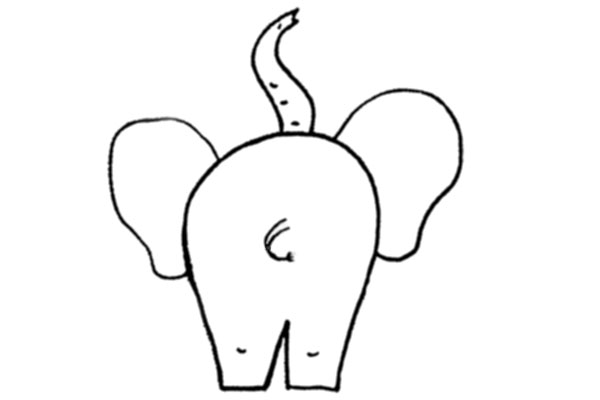
\includegraphics[scale=1.5]{images/slon.jpg}
\end{center}

\item
Укажите названия букв греческого алфавита и запишите соответствующие заглавные буквы:
\[\alpha, \zeta, \eta, \theta\].

\end{enumerate}

\subsection{Контрольная номер 1, базовый поток, 26.10.2015, решения}

\begin{enumerate}
\item
\begin{enumerate}
\item[$\alpha$)] Найдём вероятности каждого события: $\P(A) = 1/2$, $\P(B) = 1/2$, $\P(C) = 1/2$.

Проверим попарную независимость:
\begin{itemize}
\item $\P(A \cap B) = 1/4$, $\P(A) \cdot \P(B) = 1/2 \cdot 1/2 = 1/4$
\item $\P(A \cap C) = 1/4$, $\P(A) \cdot \P(C) = 1/2 \cdot 1/2 = 1/4$
\item $\P(B \cap C) = 1/4$, $\P(B) \cdot \P(C) = 1/2 \cdot 1/2 = 1/4$
\end{itemize}
Значит, события попарно независимы.
\item[$\beta$)] События $A_1, A_2, A_3$ называются независимыми в совокупности, если $\P(A_1 \cap A_2 \cap A_3) = \P(A_1) \cdot \P(A_2) \cdot \P(A_3)$.

В нашем случае: $\P(A \cap B \cap C) = 0$, $ \P(A) \cdot \P(B) \cdot \P(C) =  \frac{1}{2} \cdot \frac{1}{2} \cdot \frac{1}{2} $, следовательно, события
не являются независимыми в совокупности.
\end{enumerate}
\item
\begin{enumerate}
\item[$\alpha$)] Воспользуемся формулой полной вероятности:
\begin{multline*}
\P(\text{выпала «6»}) = \P(\text{выпала «6»} \mid \text{взят белый кубик}) \cdot \P(\text{взят белый кубик}) + \\
+ \P(\text{выпала «6»} \mid \text{взят красный кубик}) \cdot \P(\text{взят красный кубик}) = \\
= \frac{1}{6} \cdot \frac{1}{2} + \frac{1}{3} \cdot \frac{1}{2} = \frac{1}{4}
\end{multline*}
\item[$\beta$)] Воспользуемся формулой условной вероятности и результатом предыдущего пункта:
\begin{multline*}
\P(\text{взят красный кубик} \mid \text{выпала «6»}) = \frac{\P(\text{взят красный кубик} \cap \text{выпала «6»})}{\P(\text{выпала «6»})} =  \\
= \frac{\frac{1}{2}\cdot \frac{1}{3}}{\frac{1}{4}} = \frac{2}{3}
\end{multline*}
\end{enumerate}
\item
\begin{enumerate}
\item[$\alpha$)] Совместное распределение имеет вид:
\begin{center}
\begin{tabular}{@{}l|llllll@{}}
\toprule
$\eta$ $\backslash$ $\xi$ & $1$                            & $2$                            & $3$                            & $4$                            & $5$                            & $6$                            \\ \midrule
$1$           & $\frac{2}{15}\cdot\frac{1}{6}$ & $\frac{2}{15}\cdot\frac{1}{6}\mbox{*}$  & $\frac{2}{15}\cdot\frac{1}{6}\mbox{*}$   & $\frac{2}{15}\cdot\frac{1}{6} \mbox{*}$   & $\frac{2}{15}\cdot\frac{1}{6} \mbox{*}$   & $\frac{1}{3}\cdot\frac{1}{6} \mbox{*}$   \\
$2$           & $\frac{2}{15}\cdot\frac{1}{6}$ & $\frac{2}{15}\cdot\frac{1}{6}$ & $\frac{2}{15}\cdot\frac{1}{6}\mbox{*}$   & $\frac{2}{15}\cdot\frac{1}{6}\mbox{*}$   & $\frac{2}{15}\cdot\frac{1}{6}\mbox{*}$   & $\frac{1}{3}\cdot\frac{1}{6} \mbox{*}$   \\
$3$           & $\frac{2}{15}\cdot\frac{1}{6}$ & $\frac{2}{15}\cdot\frac{1}{6}$ & $\frac{2}{15}\cdot\frac{1}{6}$ & $\frac{2}{15}\cdot\frac{1}{6} \mbox{*}$   & $\frac{2}{15}\cdot\frac{1}{6} \mbox{*}$   & $\frac{1}{3}\cdot\frac{1}{6} \mbox{*}$   \\
$4$           & $\frac{2}{15}\cdot\frac{1}{6}$ & $\frac{2}{15}\cdot\frac{1}{6}$ & $\frac{2}{15}\cdot\frac{1}{6}$ & $\frac{2}{15}\cdot\frac{1}{6}$ & $\frac{2}{15}\cdot\frac{1}{6} \mbox{*}$ & $\frac{1}{3}\cdot\frac{1}{6} \mbox{*}$   \\
$5$           & $\frac{2}{15}\cdot\frac{1}{6}$ & $\frac{2}{15}\cdot\frac{1}{6}$ & $\frac{2}{15}\cdot\frac{1}{6}$ & $\frac{2}{15}\cdot\frac{1}{6}$ & $\frac{2}{15}\cdot\frac{1}{6}$ & $\frac{1}{3}\cdot\frac{1}{6} \mbox{*}$   \\
$6$           & $\frac{2}{15}\cdot\frac{1}{6}$ & $\frac{2}{15}\cdot\frac{1}{6}$ & $\frac{2}{15}\cdot\frac{1}{6}$ & $\frac{2}{15}\cdot\frac{1}{6}$ & $\frac{2}{15}\cdot\frac{1}{6}$ & $\frac{1}{3}\cdot\frac{1}{6}$ \\ \bottomrule
\end{tabular}
\end{center}
\item[$\beta$)] $\P(\text{выиграет белый кубик}) = (6 + 5 + 4 + 3 + 2) \cdot \frac{2}{15}\cdot\frac{1}{6} + 1 \cdot \frac{1}{3}\cdot\frac{1}{6} = \frac{1}{2}$.

Значит, Пете безразлично, какой кубик брать.
\item[$\gamma)$] $F_{\zeta}(x) = \P(\zeta \leq x)$

Выпишем таблицу распределения случайной величины $\zeta$:

\begin{tabular}{@{}l|cccccc@{}}
\toprule
$\zeta$     & $1$                              & $2$                                      & $3$                                      & $4$                                      & $5$                                      & $6$                                                                              \\ \midrule
$\P(\cdot)$ & $\frac{2}{15} \cdot \frac{1}{6}$ & $\frac{2}{15} \cdot \frac{1}{6} \cdot 3$ & $\frac{2}{15} \cdot \frac{1}{6} \cdot 5$ & $\frac{2}{15} \cdot \frac{1}{6} \cdot 7$ & $\frac{2}{15} \cdot \frac{1}{6} \cdot 9$ & $\frac{1}{3} \cdot \frac{1}{6} \cdot 6 + \frac{2}{15} \cdot \frac{1}{6} \cdot 5$ \\ \bottomrule
\end{tabular}

Тогда функция распределения имеет вид:
\[
F_{\zeta}(x) =
\begin{cases}
0 & x \leq 1 \\
\frac{1}{45} & 1 < x \leq 2 \\
\frac{4}{45} & 2 < x \leq 3 \\
\frac{9}{45} & 3 < x \leq 4 \\
\frac{16}{45} & 4 < x \leq 5 \\
\frac{25}{45} & 5 < x \leq 6 \\
1 & x > 6
\end{cases}
\]
\item[$\delta$)] $\E(\zeta) = \frac{2}{15} \cdot \frac{1}{6} \cdot 1 + \frac{2}{15} \cdot \frac{1}{6} \cdot 3 \cdot 2 + \frac{2}{15} \cdot \frac{1}{6} \cdot 5 \cdot 3 + \frac{2}{15} \cdot \frac{1}{6} \cdot 7 \cdot 4 + \frac{2}{15} \cdot \frac{1}{6} \cdot 9 \cdot 5 + \frac{1}{3} \cdot \frac{1}{6} \cdot 6 + \frac{2}{15} \cdot \frac{1}{6} \cdot 6 = \frac{43}{9} \approx 4.8 $
\end{enumerate}
\item Пусть $x$ — вероятность того, что мужчина честно любит петь в душе.

Распишем по формуле полной вероятности вероятность получить ответ «да»:
\begin{multline*}
P(\text{ответ «Да»}) = 1 \cdot \P(\text{выпала «6»}) + x \cdot(\P(\text{выпала «2»}) + \P(\text{выпала «3»}) +  \\
+ \P(\text{выпала «4»}) + \P(\text{выпала «5»})) = 1 \cdot \frac{1}{6} + x \cdot \frac{4}{6} \Rightarrow x = \frac{3}{4}
\end{multline*}
Тогда истинный процент «певцов» составляет $75 \%$
\item Предположим, что ваше имя — Студент (7 букв), а фамилия — Идеальный (9 букв).
\begin{enumerate}
\item[$\alpha$)] $\P(\text{напишет фаимлию правильно}) = (0.9)^9$
\item[$\beta$)] $\P(\text{ровно 2 ошибки в имени}) = C_{7}^2 \cdot 0.1^2 \cdot 0.9^5$
\item[$\gamma$)] Наиболее вероятное число ошибок — 1
\item[$\delta$)] $\P(\text{допустит хотя бы одну ошибку}) = 1 - \P(\text{не допустит ни одной ошибки}) = 1 - (0.9)^{16}$
\end{enumerate}
\item
\begin{enumerate}
\item[$\alpha$)] Из условия $\int_{0}^{1} (cy^2 + y) dy = 1$ получаем, что $c=3/2$.
\item[$\beta$)]
$F_{Y} (y) =
\begin{cases}
1 & y > 1 \\
\frac{y^3 + y^2}{2} & 0 < y \leq 1 \\
0 & y < 0
\end{cases} $
\item[$\gamma$)] $\P(Y < 0.5) = \int_{0}^{0.5} \left(\frac{3}{2} y^2 + y   \right) dy = \frac{3}{16}$
\item[$\delta$)] $F_{Y} (y) = 0.5 \Rightarrow y \approx 0.75 $
\item[$\epsilon$)] $\P(Y > 0.5 \mid Y \geq 0.25) = \frac{\P(Y > 0.5)}{\P(Y \geq 0.25)} = \frac{1 - \frac{3}{16}}{\int_{0.25}^{1} \left(\frac{3}{2} y^2 + y   \right) dy} = \frac{104}{123}$
\end{enumerate}
\item
\begin{enumerate}
\item[$\alpha$)] $\P(\text{кисточка окажется на слоне}) = \frac{1}{1.5} = \frac{2}{3}$
\item[$\beta$)] $f_{\xi, \eta}(x, y) = \frac{1}{1.5}$
\item[$\gamma$)] $f_{\xi} (x) = \int_{0}^{1} \frac{1}{1.5} dy = 1.5$

$f_{\eta}(y) = \int_{0}^{1.5} \frac{1}{1.5} dx = 1$
\item[$\delta$)] Да, поскольку $ f_{\xi} (x) \cdot f_{\eta}(y) = f_{\xi, \eta}(x, y)$
\item[$\epsilon$)] $f_{\xi+\eta} (t) = \int_{-\infty}^{+\infty} f_{\xi}(u) f_{\eta}(t-u) du $
\end{enumerate}
\end{enumerate}


\subsection{Праздник номер 1, исследователи, индивидуальный тур}

\begin{enumerate}
\item Для разминки вспомним греческий алфавит!

\begin{enumerate}
\item По-гречески — Σωκρατης, а по-русски — \underline{\hspace{2cm}}
\item Изобразите прописные и строчные буквы: эта \underline{\hspace{2cm}}, дзета \underline{\hspace{2cm}}, вега \underline{\hspace{2cm}}, шо \underline{\hspace{2cm}}. Если такой буквы в греческом нет, то поставьте прочерк.
\item Назовите буквы: τ \underline{\hspace{2cm}}, θ \underline{\hspace{2cm}}, ξ \underline{\hspace{2cm}}.
%\item Если пересчитать все буквы в греческом алфавите, то их окажется ровно \underline{\hspace{2cm}} %24
\end{enumerate}

\item Подбрасываются 2 симметричные монеты. Событие $A$ — на первой монете выпал герб, событие $B$ — на второй монете выпал герб, событие $C$ — монеты выпали разными сторонами.
\begin{enumerate}
\item Будут ли эти события попарно независимы?
\item Сформулируйте определение независимости в совокупности для трех событий
\item Являются ли события $A$, $B$, $C$ независимыми в совокупности?
\end{enumerate}


\item Имеются два игральных кубика: \textbf{красный} со смещенным центром тяжести, так что вероятность выпадения «6» равняется 1/3, а оставшиеся грани имеют равные шансы на появление и
правильный \textbf{белый} кубик.  Петя случайным образом выбирает кубик и подбрасывает его.
\begin{enumerate}
\item Вероятность того, что выпадет «6», равна \underline{\hspace{2cm}}
\item Вероятность того, что Петя взял красный кубик, если известно, что выпала шестерка, равна \underline{\hspace{2cm}}
\item Если бы в эксперименте Петя подбрасывал  бы кубик не один раз, а 60 раз, то безусловное математическое ожидание количества выпавших шестёрок равнялось бы \underline{\hspace{2cm}}
\end{enumerate}


\begin{comment}
\item Неразменный пятак всегда выпадает «орлом». У Александра Привалова в кармане один неразменный пятак и два обычных, равновероятно выпадающих «орлом» и «решкой». Привалов достаёт одну из монет наугад не глядя.
\begin{enumerate}
\item Вероятность того, что он достанет неразменный пятак равна \underline{\hspace{2cm}} % 1/3
\item Не глядя на монету, Привалов подкидывает её. Вероятность того, что она выпадет  «орлом», равна \underline{\hspace{2cm}} % 2/3
%\item Если бы эту случайную монету подкинуть не один раз, а 10, то математическое ожидание числа «орлов» равнялось бы \underline{\hspace{2cm}} % 20/3
\item Наконец Привалов глядит на упавшую монету и видит, что выпал «орёл». Вероятность того, что монета — неразменный пятак, равна \underline{\hspace{2cm}}
\end{enumerate}
\end{comment}

\item Винни-Пуху снится сон, будто он спустился в погреб, а там бесконечное количество горшков. Каждый из них независимо от других может оказаться либо пустым с вероятностью $0.8$, либо с мёдом с вероятностью $0.2$. Винни-Пух начинает перебирать горшки по очереди в поисках полного. Хотя у него в голове и опилки, Винни-Пух два раза в один и тот же горшок заглядывать не будет.
\begin{enumerate}
\item Вероятность того, что все горшки окажутся пустыми равна \underline{\hspace{2cm}}
\item Вероятность того, что полный горшок будет найден ровно с шестой попытки, равна \underline{\hspace{2cm}}
\item Вероятность того, что полный горшок будет найден на шестой попытке или ранее, равна \underline{\hspace{2cm}}
%\item Математическое ожидание числа перебранных горшков равняется \underline{\hspace{2cm}} % 5
\end{enumerate}

\item На самом деле у Винни-Пуха в погребе стоит 10 горшков. Каждый из них независимо от других может оказаться либо пустым с вероятностью $0.8$, либо с мёдом с вероятностью $0.2$.
\begin{enumerate}
\item Все десять горшков окажутся пустыми с вероятностью \underline{\hspace{2cm}}
\item Ровно $7$ горшков из десяти окажутся пустыми с вероятностью \underline{\hspace{2cm}}
\item Математическое ожидание числа горшков с мёдом равно \underline{\hspace{2cm}}
\end{enumerate}


\begin{comment}
\item Внутри треугольника с вершинами $(0,0)$, $(2,5)$ и $(8,0)$ случайно равномерно по площади выбирается точка. Пусть $X$ и $Y$ — абсцисса и ордината этой случаной точки.
\begin{enumerate}
\item Вероятность того, что $X>5$ равна \underline{\hspace{2cm}}.
\item Вероятность того, что $X>5$ и одновременно $Y<3$ равна \underline{\hspace{2cm}}.
\item Вероятность того, что $X>5$ если известно, что $Y<3$ равна \underline{\hspace{2cm}}.
\item События $X>5$ и $Y<3$ являются \underline{\hspace{1cm}}висимыми.
\item Функция плотности величины $X$ равна \underline{\hspace{2cm}}
\end{enumerate}
\end{comment}

\item В галактике Флатландии все объекты двумерные. На планету Тау-Слона (окружность) в случайных точках независимо друг от друга садятся три корабля. Любые два корабля могут поддерживать прямую связь между собой, если центральный угол между ними меньше прямого.

\begin{enumerate}
\item Вероятность того, что первый и второй корабли могут поддерживать прямую связь равна \underline{\hspace{2cm}}
\item Вероятность того, что все корабли смогут поддерживать прямую связь друг с другом равна \underline{\hspace{2cm}}
\item Вероятность того, что все корабли смогут поддерживать прямую связь друг с другом, если первый и второй корабль могут поддерживать прямую связь, равна \underline{\hspace{2cm}}
\end{enumerate}
Подсказка: во Флатландии хватит рисунка на плоскости, ведь координату третьего корабля можно принять за\ldots



\item Время (в часах), за которое студенты выполняют экзаменационное задание является случайной величиной $X$ с функцией плотности
\[
f(x)=\begin{cases}
3x^2, \, \text{ если } x \in [0;1] \\
0, \, \text{ иначе }
\end{cases}
\]

\begin{enumerate}
\item Функция распределения случайной величины $X$ равна \underline{\hspace{2cm}}
\item Вероятность того, что случайно выбранный студент закончит работу менее чем за полчаса равна \underline{\hspace{2cm}}.
\item Медиана распределения равна \underline{\hspace{2cm}}
\item Вероятность того, что студент, которому требуется по меньшей мере 15 минут для выполнения задания, справится с ним более, чем за 30 минут, равна \underline{\hspace{2cm}}
\item Функция распределения случайной величины $Y=1/X$ равна \underline{\hspace{2cm}}
\item Функция плотности случайной величины $Y=1/X$ равна \underline{\hspace{2cm}}
\end{enumerate}

\end{enumerate}

\subsection{Индивидуальный тур, решение}

\begin{enumerate}
\item Сократ, эта — Η, η, дзета — Ζ, ζ, вега — нет, шо — ϸ, τ — тау, θ — тета, ξ — кси.
Греческая буква шо, ϸ, была введена Александром Македонским и ныне вышла из употребления. По крайней мере, в греческом :) Заглавная примерно такая же, только её utf-код 03f7 не поддерживается шрифтом Linux Libertine.


\item да; события независимы в совокупности, если для любого поднабора событий $A_1$, \ldots, $A_k$ выполняется равенство $\P(A_1 \cap A_2 \cap \ldots \cap A_k) = \P(A_1) \cdot \ldots \cdot \P(A_k)$; нет
\item $1/4$, $2/3$, $15$
\item $0$, $0.8^5\cdot 0.2$, $1-0.8^6$
\item $0.8^{10}$, $C_{10}^3 0.2^3 0.8^7$, $2$
\item $1/2$, $3/16$, $3/8$
\begin{enumerate}
\item
\begin{flalign*}
F_X(x) &= \begin{cases}
0, \, x<0 \\
x^3, \, x \in [0;1] \\
1, \, x>1
\end{cases}&&
\end{flalign*}
\item $1/8$
\item $2^{-1/3}$
\item $56/63$
\item
\begin{flalign*}
F_Y(y) &= \begin{cases}
0, \, y<0 \\
1-1/y^3, \, y>0
\end{cases}&&
\end{flalign*}
\item
\begin{flalign*}
f_Y(y) &= \begin{cases}
0, \, y<0 \\
3y^{-4}, \, y>0
\end{cases}&&
\end{flalign*}

\end{enumerate}

\end{enumerate}

\subsection{Регата, исследователи, командный тур}

\begin{enumerate}
\item Восьминогий Кракен. У Кракена 8 ног-шупалец. Если отрубить одно щупальце, то в замен него с вероятностью $1/4$ вырастает новое; с вероятностью $1/4$ вырастает два новых; с вероятностью $1/2$, слава Океану, не вырастает ничего.

Против Кракена бьётся сам Капитан! Он наносит точные удары и безупречно умело уворачивается от ударов Кракена.

\begin{enumerate}
\item Какова вероятность того, что Капитан победит, отрубив ровно 10 щупалец?
\item Какова вероятность того, что бой Кракена и Капитана продлится вечно?
\item Сколько щупалец в среднем отрубит Капитан прежде чем победит?
\end{enumerate}

\item Разбавленный ром. Пират Злопамятный Джо очень любит неразбавленный ром. Из-за
того, что он много пьёт, у него проблемы с памятью, и он помнит не
больше, чем три последних пинты. Хозяин таверны с вероятностью 1/4 разбавляет
каждую подаваемую пинту рома. Если по ощущением Джо половина выпитых
пинт или больше была разбавлена, то он разносит таверну к чертям
собачьим.


\begin{enumerate}
\item Какова вероятность того, что хозяин таверны не успеет подать Джо третью пинту рома?
\item Сколько в среднем пинт выпьет Джо, прежде чем разнесёт таверну?
\end{enumerate}

\item $XY$ в степени $Z$. Чтобы поступить на службу Её Величества, пиратам предлагается следующая задача. Случайные величины $X$, $Y$ и $Z$ равномерны на отрезке $[0;1]$ и независимы.

\begin{enumerate}
\item Найдите функцию распределения случайной величины $-\ln X$
\item Найдите функцию распределения случайной величины $-(\ln X + \ln Y)$
\item Найдите функцию распределения случайной величины $-Z(\ln X + \ln Y)$
\item Какое распределение имеет случайная величина $(XY)^Z$?
\end{enumerate}

\item Тортики. Пираты очень любят тортики и праздновать день рождения! Если хотя бы у одного пирата на корабле день рождения, то все, включая капитана, празднуют и кушают тортики. Корабль в праздничный день дрейфует под действием ветра и не факт, что в нужном направлении.

\begin{enumerate}
\item Сколько пиратов нужно нанять капитану, чтобы ожидаемое количество праздничных дней было равно 100?
\item Сколько пиратов нужно нанять капитану, чтобы максимизировать ожидаемое количество рабочих пирато-дней (произведение числа пиратов на число рабочих дней)?
\end{enumerate}


\item Девятый вал. На побережье пиратского острова одна за одной набегают волны. Высота каждой волны — равномерная на $[0;1]$ случайная величина. Высоты волн независимы. Пираты называют волну «большой», если она больше предыдущей и больше следующей. Пираты называют волну «рекордной», если она больше всех предыдущих волн от начала наблюдения. Обозначим события $B_i= \{ i\text{-ая волна была большой} \}$ и $R_i=\{ i\text{-ая волна была рекордной} \}$.

\begin{enumerate}
\item Найдите $\P(R_{100})$, $\P(B_{100})$
\item Капитан насчитал 100 волн. Сколько в среднем из них были «рекордными»?
\item Найдите $\P(R_{99} | R_{100})$, $\P(R_{100}|B_{100})$
\end{enumerate}


\item Три сундука. Три пирата, Генри Рубинов, Френсис Пиастров и Эдвард Золотов играют одной командой в игру. В комнате в ряд, слева направо, стоят в случайном порядке три закрытых внешне неотличимых сундука: с рубинами, пиастрами и золотом. Общаться после начала игры они не могут, но могут заранее договориться о стратегии. Они заходят в комнату по очереди. Каждый из них может открыть два сундука по своему выбору. После каждого пирата комната возвращается уборщицей идеально точно в исходное состояние. Если Рубинов откроет коробку с рубинами, Писатров — с пиастрами, а Золотов — с золотом, то их команда выигрывает. Если хотя бы один из пиратов не найдёт свою цель, то их команда проигрывает.

\begin{enumerate}
\item Какова вероятность выигрыша, если все пираты пробуют открыть первый и второй сундуки?
\item Какова оптимальная стратегия?
\item Какова вероятность выигрыша при использовании оптимальной стратегии?
\end{enumerate}






\end{enumerate}

\subsection{Регата, исследователи, командный тур, решение}

\begin{enumerate}

\item Если отрублено 10 щупалец, значит либо был один удар породивший два новых щупальца, либо было два удара, породивших по одному новому, а все остальные удары не порождали новых щупалец.

Искомая вероятность равна: $8\cdot 0.5^9 \cdot 0.25^1 + C_8^2 0.5^8 0.25^2$.

Вероятность вечного боя равна нулю. Достаточно доказать, что с вероятностью один за конечное время побеждается одноногий Кракен. А эта вероятность удовлетворяет уравнению: $p=\frac{1}{4}p + \frac{1}{4}p^2 + \frac{1}{2} 1$. Единственный осмысленный корень у этого уравнения — $1$.

Замечаем, что на победу над $k$-шупальцевым Кракеном уходим в $k$ раз больше ударов в среднем чем на победу на $1$-щупальцевым. Отсюда:

\[
e_1=1 + 0.5\cdot 0 + 0.25\cdot e_1 + 0.25 \cdot 2e_1
\]

Решаем, получаем $e_1=4$ и $e_8=32$

\item Либо первая пинта разбавлена, либо первая неразбавлена, а вторая разбавлена, то есть
\[
0.25 + 0.75\cdot 0.25 =0.4375
\]

Рисуем граф:


Составляем систему (индекс — количество выпитых неразбавленных пинт):

\[
\begin{cases}
e_0=\frac{1}{4} + \frac{3}{16}2 + \frac{9}{16}(2+e_2) \\
e_2=1+\frac{3}{4}e_2 + \frac{1}{4}e_0
\end{cases}
\]

Находим $e_0=64/7\approx 9$

\item Начало из домашки! Для $t>0$:
\[
\P(-\ln X \leq t)=\P(\ln X > -t)=\P(X > e^{-t})=1-e^{-t}
\]

Итого,
\[
F_{-\ln X}(t)=\begin{cases}
0, \, t < 0 \\
1-e^{-t}, \, t \geq 0
\end{cases}
\]

Из геометрических соображений легко найти $\P(XY < a)$ для $a\in (0;1)$:
\[
\P(XY < a)=a + \int_a^1 \frac{a}{x} \, dx=a-a\ln a
\]

Переходим ко второму пункту, для $t>0$:
\[
\P(-(\ln X + \ln Y) < t)=\P(XY > e^{-t})= 1-e^{-t} -t e^{-t}
\]

Итого:
\[
F_{-\ln X - \ln Y}(t)=\begin{cases}
0, \, t < 0 \\
1-e^{-t} - te^{-t}, \, t \geq 0
\end{cases}
\]

После дифференциирования получаем функцию плотности для $S=-\ln X - \ln Y$:

\[
f_S(s)=\begin{cases}
0, \, s < 0 \\
se^{-s}, \, s \geq 0
\end{cases}
\]

Приближаемся к финальной вероятности:

\[
\P(ZS > t)= \int_t^{\infty} \int_{t/s}^1  se^{-s} \, dz\, ds=
\int_t^{\infty} (s-t)\cdot e^{-s} \, ds= \ldots = e^{-t}
\]

Сравниваем результат с первым пунктом и приходим к выводу, что величина $(XY)^Z$ имеет равномерное распределение на $[0;1]$.

\item Если нанято $n$ пиратов, то вероятность, того, что в конкретный день все работают равна $(364/365)^n$. Следовательно, ожидаемое количество праздничных дней равно $365(1-(364/365)^n)$.

Решаем уравнение

\[
1-(364/365)^n=100/365
\]

Получаем,
\[
n=\frac{\ln 265- \ln 365}{ \ln 364 - \ln 365}\approx 117
\]

Ожидаемое количество рабочих пирато-дней равно: $365n(364/365)^n$.

Получаем
\[
n^*=1/(\ln 365 - \ln 364)\approx 364
\]

\item
\begin{enumerate}
\item $\P(R_{100})=1/100$ (максимум из 100 величин должен плюхнуться на сотое место), $\P(B_{100})=1/3$ (максимум из трёх величин должен плюхнуться на второе место)
\item $\E(X)=1+\frac{1}{2} + \frac{1}{3}+\ldots + \frac{1}{100}\approx \ln 100 \approx 4.6$. Т.к. $X=X_1+X_2+\ldots + X_{100}$ и $\E(X_i)=1/i$.
\item $\P(R_{99} | R_{100})=1/99$, $\P(R_{100}|B_{100})=3/101$

Для проверки: $\P(R_{99} \cap R_{100})=98!/100!$ ($100!$ — всего перестановок, $98!$ — первые 98 можно переставлять свободно, а в конце должны идти второй наибольшое и наибольшее). $\P(R_{100} \cap B_{100})=1/101$ (максимум из 101 числа плюхнется на 100ое место).
\end{enumerate}

\item Если все пираты открывают первый и второй сундуки, то вероятность выигрыша равна нулю.

Оптимальная стратегия (одна из). Три пирата заранее договариваются, о названиях сундуков. Они называют эти три сундука (ещё до игры)  «рубиновым», «пиастровым» и «золотым». Генри Рубинов должен начать с открытия рубинового сундука, Френсис Пиастров — с пиастрового, Эдвард Золотов — с золотого. Далее каждый пират должен открыть тот сундук, на который указывает предмет, лежащий в первом открытом им сундуке. Например, если Генри Рубинов, открыв сначала рубиновый сундук обнаруживает там пиастры, он должен открывать пиастровый сундук.

Вероятность победы при такой стратегии легко находится перебором 6 возможных вариантов и равна\ldots Та-дам!!! $2/3$.




\end{enumerate}


\subsection{Контрольная номер 2, поток Арктура, 12.12.2015}

Продолжительность: 1 час 20 минут

\begin{enumerate}
\item Функция плотности случайного вектора $\xi=(\xi_1, \xi_2)^T$ имеет вид
\[
f(x,y)=\begin{cases}
0.5x + 1.5y, \text{ если } 0<x<1, \; 0<y<1 \\
0, \text{ иначе }
\end{cases}
\]
Найдите:
\begin{enumerate}
\item Математическое ожидание $\E(\xi_1 \cdot \xi_2)$
\item Условную плотность распределения $f_{\xi_1|\xi_2} (x|y)$
\item Условное математическое ожидание $\E(\xi_1| \xi_2=y)$
\item Константу $k$, такую, что функция $h(x,y)=kx\cdot f(x,y)$ будет являться совместной функцией плотности некоторой пары случайных величин
\end{enumerate}

\item На курсе учится очень много студентов. Вероятность того, что случайно выбранный студент по результатам рубежного контроля имеет хотя бы один незачет равна $0.2$. Пусть $\xi$ и $\eta$ — число студентов с незачетами и без незачетов в случайной группе из $10$ студентов. Найдите $\Cov(\xi,\eta)$, $\Corr(\xi,\eta)$, $\Cov(\xi-\eta,\xi)$. Являются ли случайные величины $\xi-\eta$ и $\xi$ независимыми?

\item Доходности акций компаний А и В – случайные величины $\xi$ и $\eta$. Известно, что $\E(\xi)=1$, $E(\eta)=1$, $\Var(\xi)=4$, $\Var(\eta)=9$, $\Corr(\xi,\eta)=-0.5$. Петя принимает решение потратить свой рубль на акции компании А, Вася — 50 копеек на акции компании А и 50 копеек на акции компании В, а Маша  принимает решение вложить свой рубль в портфель $R=\alpha\xi+(1-\alpha)\eta$, $(0 \leq \alpha \leq 1)$, обладающий минимальным риском. Найдите $\alpha$, ожидаемые доходности и риски портфелей Пети, Васи и Маши.

\item Будем считать, что рождение мальчика и девочки равновероятны.
\begin{enumerate}
\item Оцените с помощью неравенства Маркова вероятность того, что среди тысячи новорожденных младенцев, мальчиков будет более 75\%.
\item Оцените с помощью неравенства Чебышёва вероятность того, что доля мальчиков среди тысячи новорожденных младенцев будет отличаться от 0.5 более, чем на 0.25
\item С помощью теоремы Муавра-Лапласа вычислите вероятность из предыдущего пункта.
\end{enumerate}

\item Сейчас валютный курс племени «Мумба» составляет 100 оболов за один рубль. Изменение курса за один день — случайная величина $\delta_i$ с законом распределения:

\begin{center}
\begin{tabular}{lrrr}
\toprule
$\delta_i$ & $-1$ & $0$ & $2$ \\ \midrule
$\P(\cdot)$ & $0.25$ & $0.5$ & $0.25$ \\
\bottomrule
\end{tabular}
\end{center}

Найдите вероятность того, что через полгода (171 день) рубль будет стоить более 250 оболов, если ежедневные изменения курса происходят независимо друг от друга.

\item \textbf{Бонусная задача}

Число посетителей, зашедших в магазин в течении дня — пуассоновская случайная величина с параметром $\lambda$. Каждый из посетителей совершает покупку с вероятностью $p$, не зависимо от других посетителей. Найдите математическое ожидание числа человек, совершивших покупку.

\end{enumerate}


\subsection{Контрольная номер 2, поток Арктура, 12.12.2015, решение}

\begin{enumerate}
\item
\begin{enumerate}
\item $ \E({\xi_1 \cdot \xi_2}) = \int_{0}^1 \int_0^1 xy f(x,y) \, dx \, dy = \int_0^1 \int_0^1 \frac{1}{2}\cdot x^2y + \frac{3}{2}\cdot xy^2 \, dx \, dy = \int_{0}^1 \frac{y}{6} + \frac{3y^2}{4} \,dy = \frac{1}{3}$
\item $f_{\xi_1 | \xi_2} (x | y) = \frac{f_{\xi_1, \xi_2}(x, y)}{f_{\xi_2}(y)} = \frac{0.5x + 1.5y}{0.25 + 1.5y}, \text{ при } y \in (0,1)$
\item
\begin{multline*}
\E(\xi_1 | \xi_2 = y) = \int_0^1 x f_{\xi_1 | \xi_2} (x | y) dx = \\
= \int\limits_{0}^{1}  x \frac{0,5x + 1,5y}{0,25 + 1,5y} dx = \frac{1}{0,25 + 1,5y}  \left. \left( \dfrac{0,5x^3}{3} +  \dfrac{1,5yx^2}{2} \right) \right|_0^1  =  \frac{1/6 + 3/4y}{0,25 + 1,5y}
\end{multline*}
\item
Для того, чтобы функция являлась совместной плотностью для пары случайных величин, должно выполнятся следующее:
\[
\int_{\Omega} kx f(x,y) \, dx \, dy = 1
\]
Вычислим, чему равняется левая часть:
\[
1 = \int_{\Omega} kx f(x,y) \, dx \, dy = \int_{0}^1 \int_{0}^1 kx \left(\frac{x + 3y}{2}\right) dx \, dy = \int_{0}^1 \frac{k}{6} + \frac{3ky}{4} \, dy = \frac{k}{6} + \frac{3k}{8} \Rightarrow
\]
\[
k = \frac{24}{13}
\]
\end{enumerate}
\item Заметим, что $\xi + \eta = 10$, тогда $\Cov(\xi, \eta) = \Cov(\xi, 10-\xi) = -\Var(\xi)$.

Представим случайную величину $\xi$ в виде суммы случайных величин $\xi = \xi_1 + \ldots + \xi_{10}$, где
\[
\xi_i = \begin{cases}
1, & \text{если у студента есть хотя бы один незачёт}, p=0.2 \\
0, & \text{иначе}, p=0.8
\end{cases} \quad i = 1, \ldots, 10
\]

Поскольку результаты каждого из стуентов независимы, $\Var(\xi) = 10\Var(\xi_1)$
\[
\Cov(\xi, \eta) = -10(1^2 \cdot 0.2 - (1\cdot 0.2)^2) = -1.6
\]

Так как случайные величины $\xi$ и $\eta$ связаны соотношением $\xi = 10 - \eta$, $\Corr(\xi, \eta)=-1$.

Подставив в $\Cov(\xi - \eta, \xi)$ выражение $\eta = 10 - \xi$, получим:
\[
\Cov(\xi - \eta, \xi) = 2 \Cov(\xi, \xi) = 2 \cdot 0.16 = 0.32
\]
Случайные величины $\xi - \eta$ и $\xi$ не являются независиыми.
\item Найдем ожидаемую доходность и риск портфеля $R = \alpha \xi + (1-\alpha) \eta$ для любого $\alpha$, тогда при $\alpha = 1$ получим результаты Пети, при $\alpha = 0.5$ — результаты Васи.
\[
\E R = \alpha + (1-\alpha) = 1 \: \, \forall \, \: \alpha \in [0,1]
\]

Находим дисперсию:
\[
\Var(R) = \alpha^2 \cdot 4 + (1-\alpha)^2 \cdot 9 - 6\alpha (1-\alpha) = 19\alpha^2 -24\alpha + 9 \to \min_{\alpha} \Rightarrow
\]

Теперь, найдем оптимальное $\alpha$:
\[
\alpha = \frac{24}{38}
\]

Финальные цифры:
\[
\begin{cases}
\Var(R)^{P} = 4 \Rightarrow \sigma_{P} = 2 \\
\Var(R)^{V} = 1.75 \Rightarrow \sigma_{V} \approx 1.32 \\
\Var(R)^{M} = \frac{27}{19} \Rightarrow \sigma_{M} \approx 1.19 \\
\end{cases}
\]
\item
\begin{enumerate}
\item Пусть $S$ количество мальчиков, тогда используя \href{https://en.wikipedia.org/wiki/Markov%27s_inequality}{неравенство Маркова} получаем:
\[
\P(S \ge 750) \le \frac{\E(S)}{750} = \frac{2}{3}
\]
\item Пусть, теперь, $\overline{X}$ доля мальчиков, то есть, $\overline{X} = \sum_{i=1}^n X_i /n$, где
\[
X_i =
\begin{cases}
1, \text{ если }i\text{-ый ребёнок — мальчик }\\
0, \text{ иначе }
\end{cases}
\]
тогда используя \href{https://en.wikipedia.org/wiki/Markov%27s_inequality}{неравенство Чебышева} получаем:
\[
\P(|\overline{X} - 0.5| \ge 0.25) \le \frac{\Var(\overline{X})}{0.25^2} = \frac{1/4000}{0.25^2} = 0.004
\]
\item Вероятность из предыдущего пункта можно записать в таком виде:
\begin{multline*}
\P(|\overline{X} - 0.5| \ge 0.25) = \P(\overline{X} \ge 0.75) + \P(\overline{X} \le 0.25) = 2\P(\overline{X} \ge 0.75)=\\
= 2\P(\cN(0;1)\geq 0.25\sqrt{4000})=2\P(\cN(0;1)\geq 15.8) = 1.3 \cdot 10^{-56} \approx 0
\end{multline*}
\end{enumerate}
\item Пусть случайная величина $S$ —  это валютный курс через полгода. Заметим, что $S = 100 + \delta_1 + \ldots + \delta_{171}$.
Тогда по ЦПТ $S \sim \cN(142.75, 203.0625)$. Теперь можно искать нужную вероятность:
\[
\P(S > 250) = \P \left(\frac{S -  142.75}{\sqrt{203.0625}} > \frac{250-142.75}{\sqrt{203.0625}} \right) = \P(\cN(0, 1) > 7.6) \approx 0
\]
%\item $\lambda p$
\end{enumerate}




\subsection{Контрольная номер 2, поток Риччи, 12.12.2015}

Продолжительность: 1 час 20 минут


\begin{enumerate}
\item Функция плотности случайного вектора $\xi=(\xi_1, \xi_2)^T$ имеет вид
\[
f(x,y)=\begin{cases}
0.5x + 1.5y, \text{ если } 0<x<1, \; 0<y<1 \\
0, \text{ иначе }
\end{cases}
\]
Найдите:
\begin{enumerate}
\item Математическое ожидание $\E(\xi_1 \cdot \xi_2)$
\item Условную плотность распределения $f_{\xi_1|\xi_2} (x|y)$
\item Условное математическое ожидание $\E(\xi_1| \xi_2=y)$
\item Константу $k$, такую, что функция $h(x,y)=kx\cdot f(x,y)$ будет являться совместной функцией плотности некоторой пары случайных величин
\end{enumerate}

\item На курсе учится очень много студентов. Вероятность того, что случайно выбранный студент получит «отлично» за контрольную равна $0.2$, «хорошо» — $0.3$. Вероятности остальных результатов неизвестны. Пусть $\xi$ и $\eta$ — число отличников и хорошистов в случайной группе из $10$ студентов. Найдите $\Cov(\xi,\eta)$, $\Corr(\xi,\eta)$, $\Cov(\xi-\eta,\xi)$. Являются ли случайные величины $\xi-\eta$ и $\xi$ независимыми?

\item Доходности акций компаний А и В — случайные величины $\xi$ и $\eta$. Известно, что $\E(\xi)=1$, $E(\eta)=1$, $\Var(\xi)=4$, $\Var(\eta)=9$, $\Corr(\xi,\eta)=-0.5$. Петя принимает решение потратить свой рубль на акции компании А, Вася — 50 копеек на акции компании А и 50 копеек на акции компании В, а Маша  принимает решение вложить свой рубль в портфель $R=\alpha\xi+(1-\alpha)\eta$, $(0 \leq \alpha \leq 1)$, обладающий минимальным риском. Найдите $\alpha$, ожидаемые доходности и риски портфелей Пети, Васи и Маши.

\item Будем считать, что рождение мальчика и девочки равновероятны.
\begin{enumerate}
\item С помощью закона больших чисел определите в каком городе, большом или маленьком, больше случается таких дней, когда рождается более 75\% мальчиков.
\item Оцените с помощью неравенства Маркова вероятность того, что среди тысячи новорожденных младенцев мальчиков будет более 75\%.
\item Оцените с помощью неравенства Чебышёва вероятность того, что доля мальчиков среди тысячи новорожденных младенцев будет отличаться от 0.5 более, чем на 0.25
\item С помощью теоремы Муавра-Лапласа вычислите вероятность из предыдущего пункта.
\end{enumerate}

\item Сейчас валютный курс племени «Мумба» составляет 100 оболов за один рубль. Процентное изменение курса за один день — случайная величина $\delta_i$ с законом распределения:

\begin{center}
\begin{tabular}{lrr}
\toprule
$\delta_i$ & $-1\%$  & $1\%$ \\
$\P(\cdot)$ & $0.25$  & $0.75$ \\
\bottomrule
\end{tabular}
\end{center}

Найдите вероятность того, что через полгода (171 день) рубль будет стоить более 271 обола, если ежедневные изменения курса происходят независимо друг от друга.

\item Величины $X_1$, $X_2$, \ldots независимы и равновероятно принимают значения $-1$ и $3$.
\begin{enumerate}
\item Найдите $\plim_{n\to\infty} \frac{\sum_{i=1}^n(X_i-\bar X)^2}{n}$
\item С помощью дельта-метода найдите примерный закон распределения $\frac{\sum_{i=1}^{100}(X_i-\bar X)^2}{100}$
\end{enumerate}

\end{enumerate}

\subsection{Контрольная номер 2, поток Риччи, 12.12.2015, решение}

Решение: Аршак Минасян


\begin{enumerate}

\item
\begin{enumerate}
\item $ \E({\xi_1 \cdot \xi_2}) = \int_{0}^1 \int_0^1 xy f(x,y) \, dx \, dy = \int_0^1 \int_0^1 \frac{1}{2}\cdot x^2y + \frac{3}{2}\cdot xy^2 \, dx \, dy = \int_{0}^1 \frac{y}{6} + \frac{3y^2}{4} \,dy = \frac{1}{3}$
\item $f_{\xi_1 | \xi_2} (x | y) = \frac{f_{\xi_1, \xi_2}(x, y)}{f_{\xi_2}(y)} = \frac{0.5x + 1.5y}{0.25 + 1.5y}, \text{ при } y \in (0,1)$
\item
\begin{multline*}
\E(\xi_1 | \xi_2 = y) = \int_0^1 x f_{\xi_1 | \xi_2} (x | y) dx = \\
= \int\limits_{0}^{1}  x \frac{0,5x + 1,5y}{0,25 + 1,5y} dx = \frac{1}{0,25 + 1,5y}  \left. \left( \dfrac{0,5x^3}{3} +  \dfrac{1,5yx^2}{2} \right) \right|_0^1  =  \frac{1/6 + 3/4y}{0,25 + 1,5y}
\end{multline*}
\item
Для того, чтобы функция являлась совместной плотностью для пары случайных величин, должно выполнятся следующее:
\[
\int_{\Omega} kx f(x,y) \, dx \, dy = 1
\]
Вычислим, чему равняется левая часть:
\[
1 = \int_{\Omega} kx f(x,y) \, dx \, dy = \int_{0}^1 \int_{0}^1 kx \left(\frac{x + 3y}{2}\right) dx \, dy = \int_{0}^1 \frac{k}{6} + \frac{3ky}{4} \, dy = \frac{k}{6} + \frac{3k}{8} \Rightarrow
\]
\[
k = \frac{24}{13}
\]
\end{enumerate}
\item При расчёте ковариации применим разложение случайной величины в сумму простых случайных величин!

$\Cov(\xi, \eta) = \Cov(\xi_1 + \ldots + \xi_{10}, \eta_1 + \ldots + \eta_{10})=10\Cov(\xi_1, \eta_1)=10(0-0.2\cdot 0.3)=-0.6$

$\Var(\xi)=10\cdot 0.2\cdot 0.8=1.6 $

$\Var(\eta)=10\cdot 0.3\cdot 0.7=2.1 $

$\Corr(\xi,\eta)=-0.6/\sqrt{1.6\cdot 2.1} \approx -0.33 $

$\Cov(\xi - \eta, \xi) = \Var(\xi) - \Cov(\xi, \eta) \neq 0$

Следовательно, $\xi$ и $\eta$ зависимы.

\item Найдем ожидаемую доходность и риск портфеля $R = \alpha \xi + (1-\alpha) \eta$ для любого $\alpha$, тогда при $\alpha = 1$ получим результаты Пети, при $\alpha = 0.5$ — результаты Васи.
\[
\E R = \alpha + (1-\alpha) = 1 \: \, \forall \, \: \alpha \in [0,1]
\]

Находим дисперсию:
\[
\Var(R) = \alpha^2 \cdot 4 + (1-\alpha)^2 \cdot 9 - 6\alpha (1-\alpha) = 19\alpha^2 -24\alpha + 9 \to \min_{\alpha} \Rightarrow
\]

Теперь, найдем оптимальное $\alpha$:
\[
\alpha = \frac{24}{38}
\]

Финальные цифры:
\[
\begin{cases}
\Var(R)^{P} = 4 \Rightarrow \sigma_{P} = 2 \\
\Var(R)^{V} = 1.75 \Rightarrow \sigma_{V} \approx 1.32 \\
\Var(R)^{M} = \frac{27}{19} \Rightarrow \sigma_{M} \approx 1.19 \\
\end{cases}
\]

\item
\begin{enumerate}
\item По ЗБЧ имеем:
\[
\frac{\xi_1 + \dots + \xi_n}{n} \to \E(\xi_1) = \frac{1}{2},
\]
Поэтому, чем больше $n$ (количество жителей в городе), тем меньше таких дней, когда количество мальчиков больше $75\%.$ \\
\item Пусть $S$ количество мальчиков, тогда используя \href{https://en.wikipedia.org/wiki/Markov%27s_inequality}{неравенство Маркова} получаем:
\[
\P(S \ge 750) \le \frac{\E(S)}{750} = \frac{2}{3}
\]
\item Пусть, теперь, $\bar X$ доля мальчиков, то есть, $\overline{X} = \sum_{i=1}^n X_i /n$, где
\[
X_i =
\begin{cases}
1, \text{ если }i\text{-ый ребёнок — мальчик }\\
0, \text{ иначе }
\end{cases}
\]
тогда используя \href{https://en.wikipedia.org/wiki/Markov%27s_inequality}{неравенство Чебышева} получаем:
\[
\P(|\overline{X} - 0.5| \ge 0.25) \le \frac{\Var(\overline{X})}{0.25^2} = \frac{1/4000}{0.25^2} = 0.004
\]
\item Вероятность из предыдущего пункта можно записать в таком виде:
\begin{multline*}
\P(|\overline{X} - 0.5| \ge 0.25) = \P(\overline{X} \ge 0.75) + \P(\overline{X} \le 0.25) = 2\P(\overline{X} \ge 0.75)=\\
= 2\P(\cN(0;1)\geq 0.25\sqrt{4000})=2\P(\cN(0;1)\geq 15.8) = 1.3 \cdot 10^{-56} \approx 0
\end{multline*}
\end{enumerate}

\item

Ищем вероятность

\[
100\cdot X_1 \cdot \ldots \cdot X_{171} \geq 271
\]

Здесь $X_i$ принимают значения $0.99$ или $1.01$ с вероятностями $0.25$ и $0.75$

Берем логарифм:

\[
\sum \log X_i \geq 1
\]

Исходим из худшего случая, когда на калькуляторе нет логарифма, тогда неплохо знать, что $\log (1+\alpha) \sim \alpha$, поэтому можно считать, что $\log X_i$ принимает значения $-0.01$ и $0.01$.

Значит $\E(\log X_i)=1/200$, $\Var(\log X_i)=1/100 - 1/200^2 \approx 1/100$.

Поэтому сумма $S \sim \cN(171/200, 171/100)$ и

\[
\P(S \geq 1)=\P(\cN(0, 1) \geq 0.11) \approx 0.46
\]

\item
\begin{enumerate}
\item Используем ЗБЧ:
\[
\plim_{n \to \infty} \frac{\sum_{i=1}^n (X_i - \bar{X})^2}{n} = \plim \frac{\sum X_i^2}{n} - \plim \bar X \cdot \bar X = \E(X_1^2) - (\E(X_1))^2 = \Var(X_1) = 4
\]
\item Обозначим, $Y_i=X_i^2$, тогда наше выражение можно записать в виде:
\[
Q=\overline{Y} - (\overline{X})^2
\]

Причём, $\plim \bar Y = 5$, $\plim \bar X = 1$.

Согласно дельта-методу заменяем его на линейную аппроксимацию в окрестности предела:
\[
Q\approx 4 + (\bar Y - 5) + 2 (\bar X - 1)
\]

Стало быть, при больших $n$:

\[
\E(Q) \approx 4
\]

\begin{multline*}
\Var(Q) \approx \Var(\bar Y) + 4\Var(\bar X) + 4\Cov(\bar Y, \bar X) =\\
= \frac{1}{n} \left(\Var(Y_1) + 4 \Var(X_1) + 4\Cov(X_1, Y_1) \right) = \\
= 0.01 \cdot (16 + 4 \cdot 4 + 4 \cdot 8)= 0.64
\end{multline*}

Итого, $Q \approx \cN(4; 0.64)$

\end{enumerate}

\end{enumerate}



\subsection{Midterm, 21.12.2015}


\element{probability1}{
  \begin{questionmult}{1} %2015ready
Крошка Джон  попадает в яблочко с вероятностью $0.8$. Его выстрелы независимы. Вероятность, что он попадёт хотя бы один раз из двух равна
\begin{multicols}{3}
   \begin{choices}
      \correctchoice{$0.96$}
      \wrongchoice{$0.8$}
      \wrongchoice{$0.64$}
      \wrongchoice{$0.36$}
      \wrongchoice{$0.9$}

       \end{choices}
  \end{multicols}
  \end{questionmult}
}

\element{probability1}{
  \begin{questionmult}{2} %2015ready
Крошка Джон попадает в яблочко с вероятностью $0.8$. Его выстрелы независимы. Вероятность, что он попал оба раза, если известно, что он попал хотя бы один раз из двух, равна
   \begin{multicols}{3}
   \begin{choices}
      \correctchoice{$2/3$}
      \wrongchoice{$1/3$}
      \wrongchoice{$1/2$}
      \wrongchoice{$3/4$}
      \wrongchoice{$1/4$}

       \end{choices}
  \end{multicols}
  \end{questionmult}
}

\element{probability1}{
  \begin{questionmult}{3} %2015ready
Имеется три монетки. Две «правильных» и одна — с «орлами» по обеим сторонам. Вася выбирает одну монетку наугад и подкидывает её два раза. Вероятность того, что оба раза выпадет орел равна
    \begin{multicols}{3}
   \begin{choices}
      \correctchoice{$1/2$}
      \wrongchoice{$2/3$}
      \wrongchoice{$1/3$}
      \wrongchoice{$1/4$}
      \wrongchoice{$3/4$}

       \end{choices}
  \end{multicols}
  \end{questionmult}
}

%
% \element{probability1}{
%   \begin{questionmult}{3} %2015ready
% Крошка Джон попадает в яблочко с вероятностью $0.8$. Его выстрелы независимы. Вероятность, что он попал во второй раз, если известно, что он попал хотя бы один раз из двух, равна
%   \begin{multicols}{3}
%    \begin{choices}
%       \correctchoice{$5/6$}
%       \wrongchoice{$3/4$}
%       \wrongchoice{$2/3$}
%       \wrongchoice{$1/2$}
%       \wrongchoice{$4/5$}
%
%        \end{choices}
%   \end{multicols}
%   \end{questionmult}
% }

\element{probability1}{
  \begin{questionmult}{4} %2015ready
    Если события $A$, $B$, $C$ попарно независимы, то
    \begin{choices}
      \wrongchoice{Событие $A\cup B\cup C$ обязательно произойдёт}
      \wrongchoice{События $A$, $B$, $C$ независимы в совокупности}
      \wrongchoice{События $A$, $B$, $C$ зависимы в совокупности}
      \wrongchoice{События $A$, $B$, $C$ несовместны}
      \wrongchoice{$\P(A\cap B\cap C)=\P(A)\P(B)\P(C)$}

    \end{choices}
  \end{questionmult}
}


\element{probability1}{
  \begin{questionmult}{5} %2015ready
Случайная величина $X$ равномерна на отрезке $[0;10]$. Вероятность $\P(X>3|X<7)$ равна
    \begin{multicols}{3}
   \begin{choices}
      \correctchoice{$4/7$}
      \wrongchoice{$3/10$}
      \wrongchoice{$7/10$}
      \wrongchoice{$3/7$}
      \wrongchoice{$0.21$}

       \end{choices}
  \end{multicols}
  \end{questionmult}
}


\element{probability}{
  \begin{questionmult}{6} %2015ready
Имеется три монетки. Две «правильных» и одна — с «орлами» по обеим сторонам. Вася выбирает одну монетку наугад и подкидывает её два раза. События $A = \{ \text{Орёл выпал при первом подбрасывании} \}$ и $B =\{\text{Орёл выпал при втором подбрасывании}\}$
  \begin{multicols}{2}
   \begin{choices}
      \correctchoice{удовлетворяют соотношению $\P(A|B)\geq \P(A)$}
      \wrongchoice{независимы}
      \wrongchoice{несовместны}
      \wrongchoice{образуют полную группу событий}
       \wrongchoice{удовлетворяют соотношению $\P(A\cap B)=\P(A)+\P(B) + \P(A\cup B)$}

       \end{choices}
  \end{multicols}
  \end{questionmult}
}


\element{probability}{
  \begin{questionmult}{7} %2015ready
В квадрат вписан круг. Наудачу в квадрат бросают восемь точек. Пусть $X$ — число точек, попавших в круг. Математическое ожидание величины $X$ равно
    \begin{multicols}{3}
   \begin{choices}
      \correctchoice{$2\pi$}
      \wrongchoice{$\pi$}
      \wrongchoice{$\pi / 2$}
      \wrongchoice{$\pi / 4$}
      \wrongchoice{$4 \pi$}

       \end{choices}
  \end{multicols}
  \end{questionmult}
}


\element{probability}{
  \begin{questionmult}{8} %2015ready
В квадрат вписан круг. Наудачу в квадрат бросают восемь точек. Пусть $X$ — число точек, попавших в круг. Дисперсия величины $X$ равна    \begin{multicols}{3}
   \begin{choices}
    \correctchoice{$2\pi - \pi^2 / 2$}
      \wrongchoice{$\pi^2$}
      \wrongchoice{$\pi^2 - 2 \pi$}
      \wrongchoice{$3\pi^2 - 4$}
       \wrongchoice{$3\pi^2 - 2$}

       \end{choices}
  \end{multicols}
  \end{questionmult}
}


\element{probability}{
  \begin{questionmult}{9} %2015ready
В квадрат вписан круг. Последовательно в квадрат наудачу бросают восемь точек. Пусть $Y$ — число точек, попавших в круг, при первых четырех бросаниях, а $Z$ — число точек, попавших в круг, при оставшихся четырех бросаниях. Ковариация $\Cov(Y,Z)$ равна
    \begin{multicols}{3}
   \begin{choices}
      \correctchoice{$0$}
      \wrongchoice{$\pi^2$}
      \wrongchoice{$-\pi^2$}
      \wrongchoice{$2\pi$}
      \wrongchoice{$-2\pi$}

      \end{choices}
  \end{multicols}
  \end{questionmult}
}


\element{probability}{
  \begin{questionmult}{10} %2015ready
В квадрат вписан круг. Последовательно в квадрат наудачу бросают восемь точек. Пусть $Y$ — число точек, попавших в круг, при первых четырех бросаниях, а $Z$ — число точек, попавших в круг, при оставшихся четырех бросаниях. Дисперсия $\Var(Y - Z)$ равна
\begin{multicols}{3}
   \begin{choices}
      \correctchoice{$2\pi - \pi^2 / 2$}
      \wrongchoice{$\pi^2$}
      \wrongchoice{$\pi^2 - 2 \pi$}
      \wrongchoice{$3\pi^2 - 4$}
      \wrongchoice{ $0$}

    \end{choices}
  \end{multicols}
  \end{questionmult}
}

\element{probability}{
  \begin{questionmult}{11} %2015ready
В квадрат вписан круг. Наудачу в квадрат бросают восемь точек. Наиболее вероятное число точек, попавших в круг, равно
\begin{multicols}{3}
   \begin{choices}
      \correctchoice{$7$}
      \wrongchoice{$2\pi$}
      \wrongchoice{$4$}
      \wrongchoice{$5$}
      \wrongchoice{$6$}

    \end{choices}
  \end{multicols}
  \end{questionmult}
}


\element{probability}{
  \begin{questionmult}{12} %2015ready
Всем известно, что Маша звонит Васе в среднем 10 раз в день. Число звонков, совершенных Машей, имеет распределение Пуассона. Вероятность того, что Маша ни разу не позвонит Васе в течение дня, равна
\begin{multicols}{3}
   \begin{choices}
      \correctchoice{$e^{-10}$}
      \wrongchoice{$1 - e^{10}$}
      \wrongchoice{$10\,e^{-10}$}
      \wrongchoice{$\tfrac{1}{10!}e^{-10}$}
      \wrongchoice{$1 - e^{-10}$}

    \end{choices}
  \end{multicols}
  \end{questionmult}
}

\element{commontext}{
\newpage
\rule{\textwidth}{1pt} %2015ready
\textbf{В вопросах 13-16} совместное распределение пары величин $X$ и $Y$ задано таблицей:

\begin{center}
\begin{tabular}{c|cc}
 & $Y=-2$ & $Y=1$ \\
\hline
$X=-1$ & 0.1 & 0 \\
$X=0$ & 0.1 & 0.3 \\
$X=1$ & 0.2 & 0.3 \\
\end{tabular}
\end{center}
\vspace{0.2cm}
}

\element{1316}{
  \begin{questionmult}{13} %2015ready
Математическое ожидание величины $Y$ при условии, что $X=0$, равно
\begin{multicols}{3}
   \begin{choices}
      \correctchoice{$0.25$}
      \wrongchoice{$0$}
      \wrongchoice{$0.1$}
      \wrongchoice{$-0.1$}
      \wrongchoice{$0.2$}
      \wrongchoice{$-0.2$}

    \end{choices}
  \end{multicols}
  \end{questionmult}
}


\element{1316}{
  \begin{questionmult}{14} %2015ready
Дисперсия случайной величины $X$ равна
\begin{multicols}{3}
   \begin{choices}
      \correctchoice{$0.44$}
      \wrongchoice{$0.2$}
      \wrongchoice{$0.4$}
      \wrongchoice{$0.6$}
      \wrongchoice{$1.04$}

    \end{choices}
  \end{multicols}
  \end{questionmult}
}

\element{1316}{ %2015ready
  \begin{questionmult}{15}
Ковариация $\Cov(X, Y)$ равна
\begin{multicols}{3}
   \begin{choices}
      \correctchoice{$0.18$}
      \wrongchoice{$0.9$}
      \wrongchoice{$-0.7$}
      \wrongchoice{$-0.5$}
      \wrongchoice{$0.1$}
      \wrongchoice{$0.4$}

    \end{choices}
  \end{multicols}
  \end{questionmult}
}

\element{1316}{
  \begin{questionmult}{16} %2015ready
Вероятность того, что $Y = 1$ при условии, что $X > 0$ равна
\begin{multicols}{3}
   \begin{choices}
      \correctchoice{$0.6$}
      \wrongchoice{$0.5$}
      \wrongchoice{$0.2$}
      \wrongchoice{$0.3$}
      \wrongchoice{$0.4$}

    \end{choices}
  \end{multicols}
  \end{questionmult}
}


\element{commontext2}{ %2015ready
%\newpage
\rule{\textwidth}{1pt}
\textbf{В вопросах 17-19} Функция распределения абсолютно непрерывной случайной величины $X$ имеет вид
\[
F(x)=\begin{cases}
a, x<0,\\
b x^2+c, x \in [0,2],\\
d, x > 2.\\
\end{cases}
\]
\vspace{0.2cm}
}

\element{1719}{
  \begin{questionmult}{17} %2015ready
Величина $X$ равномерна от $0$ до $4$. Вероятность того, что $X$ примет значение 1, равна
\begin{multicols}{3}
   \begin{choices}
      \correctchoice{$0$}
      \wrongchoice{$0.25$}
      \wrongchoice{$0.4$}
      \wrongchoice{$0.5$}
      \wrongchoice{$0.8$}

    \end{choices}
  \end{multicols}
  \end{questionmult}
}

\element{1719}{
  \begin{questionmult}{18} %2015ready
Величина $X$ имеет функцию плотности $f(x)=x/2$ на отрезке $[0;2]$. Значение $\E(X)$  равно
\begin{multicols}{3}
   \begin{choices}
      \correctchoice{$4/3$}
      \wrongchoice{$0$}
      \wrongchoice{$1/2$}
      \wrongchoice{$1$}
      \wrongchoice{$2$}

    \end{choices}
  \end{multicols}
  \end{questionmult}
}

\element{1719}{
  \begin{questionmult}{19} %2015ready
Функция распределения абсолютно непрерывной случайной величины $X$ имеет вид
\[
F(x)=\begin{cases}
a, x<0,\\
b x^2+c, x \in [0,2],\\
d, x > 2.\\
\end{cases}
\]
Выражение $a+b+c+d$ равно
\begin{multicols}{3}
   \begin{choices}
      \correctchoice{$5/4$}
      \wrongchoice{$1/4$}
      \wrongchoice{$1/2$}
      \wrongchoice{$1$}
      \wrongchoice{$2$}

    \end{choices}
  \end{multicols}
  \end{questionmult}
}

\element{commontext3}{ %2015ready
\newpage
\rule{\textwidth}{1pt}
\textbf{В вопросах 20-23} совместная функция плотности пары $X$ и $Y$ имеет вид
\[
f(x,y)=\begin{cases}
(x+y)/3, \; \text{ если } x\in[0;1], y\in [0;2] \\
0, \; \text{ иначе}
\end{cases}
\]

\vspace{0.5cm}

}

\element{2023}{
  \begin{questionmult}{20} %2015ready
Если функция $h(x,y)=c\cdot x\cdot f(x,y)$ также является совместной функцией плотности, то константа $c$ равна
\begin{multicols}{3}
   \begin{choices}
      \correctchoice{$9/5$}
      \wrongchoice{$5/9$}
      \wrongchoice{$5$}
      \wrongchoice{$9$}
      \wrongchoice{$1$}
    \end{choices}
  \end{multicols}
  \end{questionmult}
}

\element{2023}{
  \begin{questionmult}{21} %2015ready
Вероятность $\P(X<0.5, Y<1)$ равна
\begin{multicols}{3}
   \begin{choices}
      \correctchoice{$1/8$}
      \wrongchoice{$5/6$}
      \wrongchoice{$3/5$}
      \wrongchoice{$5/8$}
      \wrongchoice{$3/8$}

    \end{choices}
  \end{multicols}
  \end{questionmult}
}

\element{2023}{
  \begin{questionmult}{22} %2015ready
Условная функция плотности  $f_{X|Y=1}(x)$ равна
\begin{multicols}{2}
   \begin{choices}
      \correctchoice{$f_{X|Y=1}(x)=\begin{cases} (2x+2)/3\, \text{ если } x\in [0;1] \\ 0, \text{ иначе }    \end{cases}$}
      \wrongchoice{$f_{X|Y=1}(x)=\begin{cases} (x+2)/2\, \text{ если } x\in [0;1] \\ 0, \text{ иначе }    \end{cases}$}
      \wrongchoice{$f_{X|Y=1}(x)=\begin{cases} (2x+1)/2\, \text{ если } x\in [0;1] \\ 0, \text{ иначе }    \end{cases}$}
      \wrongchoice{$f_{X|Y=1}(x)=\begin{cases} (x+4)/2\, \text{ если } x\in [0;1] \\ 0, \text{ иначе }    \end{cases}$}
      \wrongchoice{$f_{X|Y=1}(x)=\begin{cases} (4x+2)/3\, \text{ если } x\in [0;1] \\ 0, \text{ иначе }    \end{cases}$}


    \end{choices}
  \end{multicols}
  \end{questionmult}
}

\element{2023}{
  \begin{questionmult}{23} %2015ready
Математическое ожидание $\E(Y)$ равно
\begin{multicols}{3}
   \begin{choices}
      \correctchoice{$11/9$}
      \wrongchoice{$2/3$}
      \wrongchoice{$4/3$}
      \wrongchoice{$6/5$}
      \wrongchoice{$13/7$}

    \end{choices}
  \end{multicols}
  \end{questionmult}
}

\element{commontext4}{ %2015ready
%\newpage
\rule{\textwidth}{1pt}
\textbf{В вопросах 24-25} известно, что $\E(X)=-1$, $\Var(X)=1$, $\E(Y)=-4$, $\Var(Y)=4$, $\Corr(X,Y)=-0.5$

\vspace{0.5cm}

}

\element{2425}{
  \begin{questionmult}{24} %2015ready
Ковариация $\Cov(2X+Y,X-3Y)$ равна
\begin{multicols}{3}
   \begin{choices}
      \correctchoice{$-5$}
      \wrongchoice{$0$}
      \wrongchoice{$5$}
      \wrongchoice{$1$}
      \wrongchoice{$-1$}

    \end{choices}
  \end{multicols}
  \end{questionmult}
}

\element{2425}{
  \begin{questionmult}{25} %2015ready
Корреляция $\Corr((1-X)/2,(Y+5)/2)$ равна
\begin{multicols}{3}
   \begin{choices}
      \correctchoice{$0.5$}
      \wrongchoice{$-0.5$}
      \wrongchoice{$1/8$}
      \wrongchoice{$-1/8$}
      \wrongchoice{$1$}

    \end{choices}
  \end{multicols}
  \end{questionmult}
}


\element{2630}{
  \begin{questionmult}{26} %2015ready
  \AMCnoCompleteMulti
У неотрицательной случайной величины $X$ известны $\E(X)=1$, $\Var(X)=4$. Вероятность $\P(X^2 \geq 25)$ обязательно попадает в интервал
\begin{multicols}{2}
   \begin{choices}
      \correctchoice{$[0;1/5]$ }
      \wrongchoice{$[0;1/25]$}
      \wrongchoice{$[1/25;1]$}
      \wrongchoice{$[0;4/625]$}
      \wrongchoice{$[0;4/25]$}
      \wrongchoice{$[4/25;1]$}
    \end{choices}
  \end{multicols}
  \end{questionmult}
}


\element{2630}{
  \begin{questionmult}{27} %2015ready
Если $\E(X)=0$, $\Var(X)=1$, то наиболее узкий интервал, в который гарантированно попадает вероятность $\P(|X| \geq 4)$, равен

\begin{multicols}{3}
   \begin{choices}
      \correctchoice{$[0; 0.0625]$ }
      \wrongchoice{$[0.0625; 1]$}
      \wrongchoice{$[0.25; 1]$}
      \wrongchoice{$[0; 0.25]$}
      \wrongchoice{$[0.5; 1]$}

    \end{choices}
  \end{multicols}
  \end{questionmult}
}


\element{2630}{
  \begin{questionmult}{28} %2015ready
  \AMCnoCompleteMulti
Дана последовательность независимых случайных величин, имеющих равномерное на $(-1,1)$ распределение.  \textbf{НЕВЕРНЫМ} является утверждение
%\begin{multicols}{3}
   \begin{choices}
      \correctchoice{  $\bar X$ сходится по распределению к равномерной на (-1,1) величине }
      \wrongchoice{Вероятность	$\P(\bar X>0)$ стремится к 0.5}
      \wrongchoice{$\bar X$ сходится по вероятности к нулю}
      \wrongchoice{	$\sqrt{3n}\bar X$ сходится по распределению к стандартной нормальной величине}
      \wrongchoice{Вероятность	$\P(\bar X = 0)$ стремится к 0}
      \wrongchoice{	$\P(|\bar X|<1/\sqrt{n})\leq 1/3$ }
    \end{choices}
%  \end{multicols}
  \end{questionmult}
}

\element{2630}{
  \begin{questionmult}{29} %2015ready
  \AMCnoCompleteMulti
Функция плотности случайной величины $X$ имеет вид
\[
f(x)=\frac{1}{\sqrt{8\pi}} e^{-(x-3)^2/8}
\]
 \textbf{НЕВЕРНЫМ} является утверждение
\begin{multicols}{3}
   \begin{choices}
      \correctchoice{$\Var(X)=8$ }
      \wrongchoice{$\max f(x) = \frac{1}{2\sqrt{2\pi}}$}
      \wrongchoice{$\E(X)=3$}
      \wrongchoice{$\P(X>3)=0.5$}
      \wrongchoice{$\P(X=0)=0$}
      \wrongchoice{$\P(X<0)>0$}
    \end{choices}
  \end{multicols}
  \end{questionmult}
}

\element{2630}{
  \begin{questionmult}{30}
Величины $X_1$, $X_2$, \ldots независимы и одинаково распределены с $\E(X_i)=\mu$, $\Var(X_i)=\sigma^2$. К стандартному нормальному распределению  сходится последовательность случайных величин
\begin{multicols}{3}
   \begin{choices}
      \correctchoice{$\sqrt{n}(\bar X - \mu) /\sigma$ }
      \wrongchoice{$\bar X$}
      \wrongchoice{$(\bar X - \mu) /\sigma$}
      \wrongchoice{$(\bar X - \mu) /(\sqrt{n}\sigma)$}
       \wrongchoice{$(\bar X - n\mu) /(\sqrt{n}\sigma)$}
    \end{choices}
  \end{multicols}
  \end{questionmult}
}

\element{ruler}{
\noindent\rule{\textwidth}{1pt}
}

\element{newpage}{
\newpage\null
}



\element{exam_15}{
  \begin{questionmult}{1}
Пусть $X_1$, \ldots, $X_n$ — выборка объема $n$ из равномерного на $[a, b]$ распределения. Оценка $X_1+X_2$ параметра $c=a+b$ является
\begin{multicols}{2}
   \begin{choices}
      \correctchoice{несмещенной и несостоятельной}
      \wrongchoice{несмещенной и состоятельной}
      \wrongchoice{смещенной и состоятельной}
      \wrongchoice{смещенной и несостоятельной}
      \wrongchoice{асимптотически несмещенной и состоятельной}
      \end{choices}
  \end{multicols}
  \end{questionmult}
}


\element{exam_15}{
  \begin{questionmult}{2}
Пусть $X_1$, \ldots, $X_n$ — выборка объема $n$ из некоторого распределения с конечным математическим ожиданием. Несмещенной и состоятельной оценкой математического ожидания является
\begin{multicols}{3}
   \begin{choices}
      \correctchoice{$\frac{X_1}{2 n}+\frac{X_2+\ldots+X_{n-1}}{n-2}-\frac{X_n}{2 n}$}
      \wrongchoice{$\frac{1}{3} X_1 + \frac{2}{3} X_2$}
      \wrongchoice{$\frac{X_1}{2 n}+\frac{X_2+\ldots+X_{n-2}}{n-2}+\frac{X_n}{2 n}$}
      \wrongchoice{$\frac{X_1}{2 n}+\frac{X_2+\ldots+X_{n-2}}{n-1}+\frac{X_n}{2 n}$}
      \wrongchoice{$\frac{X_1+X_2}{2}$}
      \end{choices}
  \end{multicols}
  \end{questionmult}
}

\element{exam_15}{
  \begin{questionmult}{3}
Пусть $X_1$,\ldots, $X_n$ — выборка объема $n$ из равномерного на $[0, \theta]$ распределения. Оценка параметра $\theta$ методом моментов по $k$-му моменту имеет вид:
\begin{multicols}{3}
   \begin{choices}
      \correctchoice{$\sqrt[k]{(k+1) \overline{X^k}}$}
      \wrongchoice{$\sqrt[k]{(k+1) \overline{X}^k}$}
      \wrongchoice{$\sqrt[k]{k \overline{X^k}}$}
      \wrongchoice{$\sqrt[k]{k \overline{X}^k}$}
       \wrongchoice{$\sqrt[k+1]{(k+1) \overline{X}^k}$}
      \end{choices}
  \end{multicols}
  \end{questionmult}
}


\element{exam_15}{
  \begin{questionmult}{4}
Пусть $X_1$, \ldots, $X_n$ — выборка объема $n$ из равномерного на $[0, \theta]$ распределения. Состоятельной оценкой параметра $\theta$ является:
\begin{multicols}{3}
   \begin{choices}[o] % не рандомизирует порядок ответов
      \wrongchoice{$X_{(n)}$}
      \wrongchoice{$X_{(n-1)}$}
      \wrongchoice{$\frac{n}{n+1} X_{(n-1)}$}
       \wrongchoice{$\frac{n^2}{n^2-n+3} X_{(n-3)}$}
       \correctchoice{все перечисленные случайные величины}
      \end{choices}
  \end{multicols}
  \end{questionmult}
}


\element{exam_15}{ % в фигурных скобках название группы вопросов
  \begin{questionmult}{5} % тип вопроса (questionmult — множественный выбор) и в фигурных — номер вопроса
Пусть $X_1$, \ldots, $X_{2 n}$ — выборка объема $2 n$ из некоторого распределения. Какая из нижеперечисленных оценок математического ожидания имеет наименьшую дисперсию?
\begin{multicols}{3} % располагаем ответы в 3 колонки
   \begin{choices} % опция [o] не рандомизирует порядок ответов
      \wrongchoice{$X_1$}
      \wrongchoice{$\frac{X_1+X_2}{2}$}
      \wrongchoice{$\frac{1}{n} \sum_{i=1}^n X_i$}
       \wrongchoice{$\frac{1}{n} \sum_{i=n+1}^{2 n} X_i$}
       \correctchoice{$\frac{1}{2 n} \sum_{i=1}^{2 n} X_i$}
      \end{choices}
  \end{multicols}
  \end{questionmult}
}


\element{exam_15}{ % в фигурных скобках название группы вопросов
  \begin{questionmult}{6} % тип вопроса (questionmult — множественный выбор) и в фигурных — номер вопроса
Пусть $X_1$, \ldots, $X_n$ — выборка объема $n$ из распределения Бернулли с параметром $p$. Статистика $X_2 X_{n-2}$ является
\begin{multicols}{2} % располагаем ответы в [k] колонки
   \begin{choices} % опция [o] не рандомизирует порядок ответов
      \wrongchoice{оценкой максимального правдоподобия}
      \wrongchoice{асимптотически нормальной оценкой $p^2$}
      \wrongchoice{эффективной оценкой $p^2$}
       \wrongchoice{состоятельной оценкой $p^2$}
       \correctchoice{несмещенной оценкой $p^2$}
      \end{choices}
  \end{multicols}
  \end{questionmult}
}

\element{exam_15}{ % в фигурных скобках название группы вопросов
  \begin{questionmult}{7} % тип вопроса (questionmult — множественный выбор) и в фигурных — номер вопроса
Пусть $X_1$, \ldots, $X_n$ — выборка объема $n$ из равномерного на $[a, b]$ распределения. Выберите наиболее точный ответ из предложенных. Оценка $\theta^*_n = X_{(n)}-X_{(1)}$ длины отрезка $[a,b]$ является
\begin{multicols}{3} % располагаем ответы в 3 колонки
   \begin{choices} % опция [o] не рандомизирует порядок ответов
      \wrongchoice{несмещенной}
      \wrongchoice{состоятельной и асимптотически смещённой}
      \wrongchoice{несостоятельной и асимптотически несмещенной}
       \wrongchoice{нормально распределённой}
       \correctchoice{состоятельной и асимптотически несмещенной}
      \end{choices}
  \end{multicols}
  \end{questionmult}
}


\element{exam_15}{ % в фигурных скобках название группы вопросов
  \begin{questionmult}{8} % тип вопроса (questionmult — множественный выбор) и в фигурных — номер вопроса
Мощностью теста называется
%\begin{multicols}{2} % располагаем ответы в [k] колонки
   \begin{choices} % опция [o] не рандомизирует порядок ответов
      \wrongchoice{Вероятность отвергнуть основную гипотезу, когда она верна}
      \wrongchoice{Вероятность отвергнуть альтернативную гипотезу, когда она верна}
      \wrongchoice{Вероятность принять неверную гипотезу}
       \wrongchoice{Единица минус  вероятность отвергнуть основную гипотезу, когда она верна}
       \correctchoice{Единица минус  вероятность отвергнуть альтернативную гипотезу, когда она верна}
      \end{choices}
%  \end{multicols}
  \end{questionmult}
}

\element{exam_15}{ % в фигурных скобках название группы вопросов
  \begin{questionmult}{9} % тип вопроса (questionmult — множественный выбор) и в фигурных — номер вопроса
Если P-значение (P-value) больше уровня значимости  $\alpha$, то гипотеза  $H_0: \; \sigma=1$
\begin{multicols}{2} % располагаем ответы в {k} колонки
   \begin{choices} % опция [o] не рандомизирует порядок ответов
      \wrongchoice{Отвергается}
      \wrongchoice{Отвергается, только если  $H_a: \; \sigma>1$}
      \wrongchoice{Отвергается, только если  $H_a: \; \sigma\neq 1$}
       \wrongchoice{ Отвергается, только если  $H_a: \; \sigma<1$}
       \correctchoice{Не отвергается}
      \end{choices}
  \end{multicols}
  \end{questionmult}
}


\element{exam_15}{ % в фигурных скобках название группы вопросов
  \begin{questionmult}{10} % тип вопроса (questionmult — множественный выбор) и в фигурных — номер вопроса
Имеется случайная выборка размера $n$ из нормального распределения. При проверке гипотезы о равенстве математического ожидания заданному значению при известной дисперсии используется статистика, имеющая распределение
\begin{multicols}{3} % располагаем ответы в {k} колонки
   \begin{choices} % опция [o] не рандомизирует порядок ответов
      \wrongchoice{$t_n$}
      \wrongchoice{ $t_{n-1}$}
      \wrongchoice{$\chi^2_n$}
       \wrongchoice{$\chi^2_{n-1}$}
       \correctchoice{$N(0,1)$}
      \end{choices}
  \end{multicols}
  \end{questionmult}
}




\element{exam_15}{ % в фигурных скобках название группы вопросов
  \begin{questionmult}{11} % тип вопроса (questionmult — множественный выбор) и в фигурных — номер вопроса
Имеется случайная выборка размера $n$ из нормального распределения. При проверке гипотезы о равенстве дисперсии заданному значению при неизвестном математическом ожидании используется статистика, имеющая распределение
\begin{multicols}{3} % располагаем ответы в {k} колонки
   \begin{choices} % опция [o] не рандомизирует порядок ответов
      \wrongchoice{$t_n$}
      \wrongchoice{ $t_{n-1}$}
      \wrongchoice{$\chi^2_n$}
       \wrongchoice{$N(0,1)$}
       \correctchoice{$\chi^2_{n-1}$}
      \end{choices}
  \end{multicols}
  \end{questionmult}
}


\element{exam_15}{ % в фигурных скобках название группы вопросов
  \begin{questionmult}{12} % тип вопроса (questionmult — множественный выбор) и в фигурных — номер вопроса
По случайной выборке из 100 наблюдений было оценено выборочное среднее $\bar{X}=20$  и несмещенная оценка дисперсии  $\hat{\sigma}^2=25$. В рамках проверки гипотезы $H_0: \; \mu=15$  против альтернативной гипотезы $H_a: \; \mu>15$  можно сделать следующее заключение
%\begin{multicols}{2} % располагаем ответы в {k} колонки
   \begin{choices} % опция [o] не рандомизирует порядок ответов
      \wrongchoice{Гипотеза $H_0$  отвергается на уровне значимости 5\%, но не  на уровне значимости 1\%}
      \wrongchoice{Гипотеза  $H_0$ отвергается на уровне значимости 10\%, но не на уровне значимости 5\%}
      \wrongchoice{Гипотеза  $H_0$ отвергается на уровне значимости 20\%, но не  на уровне значимости 10\%}
       \wrongchoice{ Гипотеза $H_0$  не отвергается на любом разумном уровне значимости}
       \correctchoice{Гипотеза $H_0$  отвергается на любом разумном уровне значимости}
      \end{choices}
%  \end{multicols}
  \end{questionmult}
}


\element{exam_15}{ % в фигурных скобках название группы вопросов
  \begin{questionmult}{13} % тип вопроса (questionmult — множественный выбор) и в фигурных — номер вопроса
На основе случайной выборки, содержащей одно наблюдение  $X_1$, тестируется гипотеза $H_0: \; X_1 \sim U[0;1]$  против альтернативной гипотезы  $H_a: \; X_1 \sim U[0.5;1.5]$. Рассматривается критерий: если $X_1>0.8$, то гипотеза $H_0$  отвергается в пользу гипотезы  $H_a$. Вероятность ошибки 2-го рода для этого критерия равна:
\begin{multicols}{3} % располагаем ответы в {k} колонки
   \begin{choices} % опция [o] не рандомизирует порядок ответов
      \wrongchoice{0.1}
      \wrongchoice{0.2}
      \wrongchoice{0.4}
       \wrongchoice{0.5}
       \correctchoice{0.3}
      \end{choices}
 \end{multicols}
  \end{questionmult}
}

\element{exam_15}{ % в фигурных скобках название группы вопросов
  \begin{questionmult}{14} % тип вопроса (questionmult — множественный выбор) и в фигурных — номер вопроса
Пусть $X_1$, $X_2$, \ldots, $X_n$ — случайная выборка размера 36 из нормального распределения $N(\mu, 9)$. Для тестирования основной гипотезы  $H_0: \; \mu=0$  против альтернативной $H_a: \; \mu=-2$   вы используете критерий: если  $\bar{X}\geq -1$, то вы не отвергаете гипотезу $H_0$, в противном случае вы отвергаете гипотезу  $H_0$ в пользу гипотезы  $H_a$. Мощность критерия равна
\begin{multicols}{3} % располагаем ответы в {k} колонки
   \begin{choices} % опция [o] не рандомизирует порядок ответов
      \wrongchoice{0.58}
      \wrongchoice{0.85}
      \wrongchoice{0.78}
       \wrongchoice{0.87}
       \correctchoice{0.98}
      \end{choices}
 \end{multicols}
  \end{questionmult}
}

\element{exam_15}{ % в фигурных скобках название группы вопросов
  \begin{questionmult}{15} % тип вопроса (questionmult — множественный выбор) и в фигурных — номер вопроса
Николай Коперник подбросил бутерброд 200 раз. Бутерброд упал маслом вниз 95 раз, а маслом вверх — 105 раз. Значение критерия $\chi^2$ Пирсона для проверки гипотезы о равной вероятности данных событий равно
\begin{multicols}{3} % располагаем ответы в {k} колонки
   \begin{choices} % опция [o] не рандомизирует порядок ответов
      \wrongchoice{0.25}
      \wrongchoice{0.75}
      \wrongchoice{0.5}
       \wrongchoice{7.5}
       \correctchoice{0.5}
      \end{choices}
 \end{multicols}
  \end{questionmult}
}

\element{exam_15}{ % в фигурных скобках название группы вопросов
  \begin{questionmult}{16} % тип вопроса (questionmult — множественный выбор) и в фигурных — номер вопроса
Каждое утро в 8:00 Иван Андреевич Крылов, либо завтракает, либо уже позавтракал. В это же время кухарка либо заглядывает к Крылову, либо нет. По таблице сопряженности вычислите  статистику $\chi^2$ Пирсона для тестирования гипотезы о том, что визиты кухарки не зависят от того, позавтракал ли уже Крылов или нет.
\begin{tabular}{c|cc}
Время 8:00 & кухарка заходит & кухарка не заходит \\
\hline
Крылов завтракает & 200 & 40 \\
Крылов уже позавтракал & 25 & 100 \\
\end{tabular}
\begin{multicols}{3} % располагаем ответы в {k} колонки
   \begin{choices} % опция [o] не рандомизирует порядок ответов
      \wrongchoice{39}
      \wrongchoice{79}
      \wrongchoice{100}
       \wrongchoice{179}
       \correctchoice{139}
      \end{choices}
 \end{multicols}
  \end{questionmult}
}

%% Боря Демешев:

\element{exam_15}{ % в фигурных скобках название группы вопросов
  \begin{questionmult}{17} % тип вопроса (questionmult — множественный выбор) и в фигурных — номер вопроса
Ковариационная матрица вектора $X=(X_1,X_2)$ имеет вид
\[
\begin{pmatrix}
10 & 3 \\
3 & 8
\end{pmatrix}
\]
Дисперсия разности элементов вектора, $\Var(X_1-X_2)$, равняется
\begin{multicols}{3} % располагаем ответы в {k} колонки
   \begin{choices} % опция [o] не рандомизирует порядок ответов
      \wrongchoice{18}
      \wrongchoice{15}
      \wrongchoice{2}
       \wrongchoice{6}
       \correctchoice{12}
      \end{choices}
 \end{multicols}
  \end{questionmult}
}


\element{exam_15}{ % в фигурных скобках название группы вопросов
  \begin{questionmult}{18} % тип вопроса (questionmult — множественный выбор) и в фигурных — номер вопроса
Все условия регулярности для применения метода максимального правдоподобия выполнены. Вторая производная лог-функции правдоподобия равна $\ell''(\hat{\theta})=-100$. Оценка стандартной ошибки для $\hat{\theta}$ равна
\begin{multicols}{3} % располагаем ответы в {k} колонки
   \begin{choices} % опция [o] не рандомизирует порядок ответов
      \wrongchoice{100}
      \wrongchoice{10}
      \wrongchoice{1}
       \wrongchoice{0.01}
       \correctchoice{0.1}
      \end{choices}
 \end{multicols}
  \end{questionmult}
}

\element{exam_15}{ % в фигурных скобках название группы вопросов
  \begin{questionmult}{19} % тип вопроса (questionmult — множественный выбор) и в фигурных — номер вопроса
Геродот Геликарнасский проверяет гипотезу $H_0: \; \mu=0, \; \sigma^2=1$ с помощью $LR$ статистики теста отношения правдоподобия. При подстановке оценок метода максимального правдоподобия в лог-функцию правдоподобия он получил $\ell=-177$, а при подстановке $\mu=0$ и $\sigma=1$ оказалось, что $\ell=-211$. Найдите значение $LR$ статистики и укажите её закон распределения при верной $H_0$
\begin{multicols}{3} % располагаем ответы в {k} колонки
   \begin{choices} % опция [o] не рандомизирует порядок ответов
      \wrongchoice{$LR=34$, $\chi^2_2$}
      \wrongchoice{$LR=34$, $\chi^2_{n-1}$}
      \wrongchoice{$LR=\ln 68$, $\chi^2_{n-2}$}
       \wrongchoice{$LR=\ln 34$, $\chi^2_{n-2}$}
       \correctchoice{$LR=68$, $\chi^2_2$}
      \end{choices}
 \end{multicols}
  \end{questionmult}
}


\element{exam_15}{ % в фигурных скобках название группы вопросов
  \begin{questionmult}{20} % тип вопроса (questionmult — множественный выбор) и в фигурных — номер вопроса
Геродот Геликарнасский проверяет гипотезу $H_0: \; \mu=2$. Лог-функция правдоподобия имеет вид $\ell(\mu,\nu)=-\frac{n}{2}\ln (2\pi)-\frac{n}{2}\ln \nu -\frac{\sum_{i=1}^n(x_i-\mu)^2}{2\nu}$. Оценка максимального правдоподобия для $\nu$ при предположении, что $H_0$ верна, равна
\begin{multicols}{3} % располагаем ответы в {k} колонки
   \begin{choices} % опция [o] не рандомизирует порядок ответов
      \wrongchoice{$\frac{\sum x_i^2 - 4\sum x_i}{n}$}
      \wrongchoice{$\frac{\sum x_i^2 - 4\sum x_i}{n}+1$}
      \wrongchoice{$\frac{\sum x_i^2 - 4\sum x_i}{n}+2$}
       \wrongchoice{$\frac{\sum x_i^2 - 4\sum x_i}{n}+3$}
       \correctchoice{$\frac{\sum x_i^2 - 4\sum x_i}{n}+4$}
      \end{choices}
 \end{multicols}
  \end{questionmult}
}


\element{exam_15}{ % в фигурных скобках название группы вопросов
  \begin{questionmult}{21} % тип вопроса (questionmult — множественный выбор) и в фигурных — номер вопроса
Ацтек Монтесума Илуикамина хочет оценить параметр $a$ методом максимального правдоподобия по выборке из неотрицательного распределения с функцией плотности $f(x)=\frac{1}{2}a^3x^2e^{-ax}$ при $x\geq 0$. Для этой цели ему достаточно максимизировать функцию
\begin{multicols}{3} % располагаем ответы в {k} колонки
   \begin{choices} % опция [o] не рандомизирует порядок ответов
      \wrongchoice{$3n\ln a - a \prod \ln x_i$}
      \wrongchoice{$3n\prod \ln a - a x^n$}
      \wrongchoice{$3n \ln a - an \ln x_i$}
       \wrongchoice{$3n \sum \ln a_i - a \sum \ln x_i$}
       \correctchoice{$3n \ln a - a \sum x_i$}
      \end{choices}
 \end{multicols}
  \end{questionmult}
}

\element{exam_15}{ % в фигурных скобках название группы вопросов
  \begin{questionmult}{22} % тип вопроса (questionmult — множественный выбор) и в фигурных — номер вопроса
Бессмертный гений поэзии Ли Бо оценивает математическое ожидание  по выборка размера $n$ из нормального распределения. Он построил оценку метода моментов, $\hat{\mu}_{MM}$, и оценку максимального правдоподобия, $\hat{\mu}_{ML}$. Про эти оценки можно утверждать, что
\begin{multicols}{2} % располагаем ответы в {k} колонки
   \begin{choices} % опция [o] не рандомизирует порядок ответов
      \wrongchoice{они не равны, но сближаются при $n\to \infty$}
      \wrongchoice{они не равны, и не сближаются при $n\to \infty$}
      \wrongchoice{ $\hat{\mu}_{MM}>\hat{\mu}_{ML}$}
       \wrongchoice{$\hat{\mu}_{MM}<\hat{\mu}_{ML}$ }
       \correctchoice{они равны}
      \end{choices}
 \end{multicols}
  \end{questionmult}
}


%% Ваня Станкевич

\element{exam_15}{ % в фигурных скобках название группы вопросов
  \begin{questionmult}{23} % тип вопроса (questionmult — множественный выбор) и в фигурных — номер вопроса
Проверяя гипотезу о равенстве дисперсий в двух выборках (размером в 3 и 5 наблюдений), Анаксимандр Милетский получил значение тестовой статистики 10. Если оценка дисперсии по первой выборке равна 8, то вторая оценка дисперсии может быть равна
\begin{multicols}{3} % располагаем ответы в {k} колонки
   \begin{choices} % опция [o] не рандомизирует порядок ответов
      \wrongchoice{$25$}
      \wrongchoice{$4/3$}
      \wrongchoice{$3/4$}
       \wrongchoice{$4$}
       \correctchoice{$80$}
      \end{choices}
 \end{multicols}
  \end{questionmult}
}

\element{exam_15}{ % в фигурных скобках название группы вопросов
  \begin{questionmult}{24} % тип вопроса (questionmult — множественный выбор) и в фигурных — номер вопроса
Пусть  $\hat{\sigma}^2_1$ — несмещенная оценка дисперсии, полученная по первой выборке размером $n_1$,   $\hat{\sigma}^2_2$ — несмещенная оценка дисперсии, полученная по второй выборке, с меньшим размером  $n_2$. Тогда статистика $\frac{\hat{\sigma}^2_1/n_1}{\hat{\sigma}^2_2/n_2}$  имеет распределение
\begin{multicols}{3} % располагаем ответы в {k} колонки
   \begin{choices} % опция [o] не рандомизирует порядок ответов
      \wrongchoice{$N(0;1)$}
      \wrongchoice{$\chi^2_{n_1+n_2}$}
      \wrongchoice{$F_{n_1,n_2}$}
       \wrongchoice{$t_{n_1+n_2-1}$}
       \wrongchoice{$F_{n_1-1,n_2-1}$}
      \end{choices}
 \end{multicols}
  \end{questionmult}
}

\element{exam_15}{ % в фигурных скобках название группы вопросов
  \begin{questionmult}{25} % тип вопроса (questionmult — множественный выбор) и в фигурных — номер вопроса
Зулус Чака каСензангакона проверяет гипотезу  о равенстве математических ожиданий в двух нормальных выборках небольших размеров $n_1$   и  $n_2$. Если дисперсии неизвестны, но равны, то тестовая статистика имеет распределение
\begin{multicols}{3} % располагаем ответы в {k} колонки
   \begin{choices} % опция [o] не рандомизирует порядок ответов
      \wrongchoice{$t_{n_1+n_2-2}$}
      \wrongchoice{$t_{n_1+n_2}$}
      \wrongchoice{$F_{n_1,n_2}$}
       \correctchoice{$t_{n_1+n_2-1}$}
       \wrongchoice{$\chi^2_{n_1+n_2-1}$}
      \end{choices}
 \end{multicols}
  \end{questionmult}
}

\element{exam_15}{ % в фигурных скобках название группы вопросов
  \begin{questionmult}{26} % тип вопроса (questionmult — множественный выбор) и в фигурных — номер вопроса
Критерий знаков проверяет нулевую гипотезу
%\begin{multicols}{3} % располагаем ответы в {k} колонки
   \begin{choices} % опция [o] не рандомизирует порядок ответов
      \wrongchoice{о равенстве математических ожиданий двух нормально распределенных случайных величин}
      \wrongchoice{о совпадении функции распределения случайной величины с заданной теоретической функцией распределения}
      \wrongchoice{о равенстве нулю вероятности того, что случайная величина $X$ окажется больше случайной величины $Y$, если альтернативная гипотеза записана как $\mu_X>\mu_Y$ }
       \correctchoice{о равенстве нулю вероятности того, что случайная величина $X$ окажется больше случайной величины $Y$, если альтернативная гипотеза записана как $\mu_X>\mu_Y$}
       \wrongchoice{о равенстве $1/2$ вероятности того, что случайная величина $X$ окажется больше случайной величины $Y$, если альтернативная гипотеза записана как $\mu_X>\mu_Y$}
      \end{choices}
% \end{multicols}
  \end{questionmult}
}


\element{exam_15}{ % в фигурных скобках название группы вопросов
  \begin{questionmult}{27} % тип вопроса (questionmult — множественный выбор) и в фигурных — номер вопроса
Вероятность ошибки первого рода, $\alpha$, и вероятность ошибки второго рода, $\beta$, всегда связаны соотношением
\begin{multicols}{3} % располагаем ответы в {k} колонки
   \begin{choices} % опция [o] не рандомизирует порядок ответов
      \wrongchoice{$\alpha+\beta=1$}
      \wrongchoice{$\alpha+\beta \leq 1$}
      \wrongchoice{$\alpha+\beta \geq 1$}
       \wrongchoice{$\alpha\leq \beta $}
       \wrongchoice{$\alpha\geq \beta $}
      \end{choices}
 \end{multicols}
  \end{questionmult}
}


\element{exam_15}{ % в фигурных скобках название группы вопросов
  \begin{questionmult}{28} % тип вопроса (questionmult — множественный выбор) и в фигурных — номер вопроса
Среди 100 случайно выбранных ацтеков 20 платят дань Кулуакану, а 80 — Аскапоцалько. Соответственно, оценка доли ацтеков, платящих дань Кулуакану, равна $\hat{p}=0.2$. Разумная оценка стандартного отклонения случайной величины $\hat{p}$ равна
\begin{multicols}{3} % располагаем ответы в {k} колонки
   \begin{choices} % опция [o] не рандомизирует порядок ответов
      \wrongchoice{$0.4$}
      \wrongchoice{$0.16$}
      \wrongchoice{$1.6$}
       \wrongchoice{$0.016$}
       \correctchoice{$0.04$}
      \end{choices}
 \end{multicols}
  \end{questionmult}
}



%% ЕВ Коссова

\element{exam_15}{ % в фигурных скобках название группы вопросов
  \begin{questionmult}{29} % тип вопроса (questionmult — множественный выбор) и в фигурных — номер вопроса
Датчик случайных чисел выдал следующие значения псевдо случайной величины: $0.78$, $0.48$. Вычислите значение критерия Колмогорова и проверьте гипотезу $H_0$ о соответствии распределения равномерному на $[0;1]$. Критическое значение статистики Колмогорова для уровня значимости 0.1 и двух наблюдений равно $0.776$.
\begin{multicols}{3} % располагаем ответы в {k} колонки
   \begin{choices} % опция [o] не рандомизирует порядок ответов
      \wrongchoice{0.3, $H_0$ не отвергается}
      \wrongchoice{1.26, $H_0$ отвергается}
      \wrongchoice{0.48, $H_0$ не отвергается}
       \wrongchoice{0.37, $H_0$ не отвергается}
       \correctchoice{0.78, $H_0$ отвергается}
      \end{choices}
 \end{multicols}
  \end{questionmult}
}

\element{exam_15}{ % в фигурных скобках название группы вопросов
  \begin{questionmult}{30} % тип вопроса (questionmult — множественный выбор) и в фигурных — номер вопроса
У пяти случайно выбранных студентов первого потока результаты за контрольную по статистике оказались равны  82, 47, 20, 43 и 73. У четырёх случайно выбранных студентов второго потока — 68, 83, 60 и 52. Вычислите статистику Вилкоксона и проверьте гипотезу $H_0$ об однородности результатов студентов двух потоков. Критические значения статистики Вилкоксона равны $T_L=12$ и $T_R=28$.
\begin{multicols}{3} % располагаем ответы в {k} колонки
   \begin{choices} % опция [o] не рандомизирует порядок ответов
      \wrongchoice{20, $H_0$ не отвергается}
      \wrongchoice{65.75, $H_0$ отвергается}
      \wrongchoice{53, $H_0$ отвергается}
       \wrongchoice{12.75, $H_0$ не отвергается}
       \correctchoice{24, $H_0$ не отвергается}
      \end{choices}
 \end{multicols}
  \end{questionmult}
}

\element{exam_15}{ % в фигурных скобках название группы вопросов
  \begin{questionmult}{31} % тип вопроса (questionmult — множественный выбор) и в фигурных — номер вопроса
 Производитель мороженного попросил оценить по 10-бальной шкале два вида мороженного: с кусочками шоколада и с орешками. Было опрошено 5 человек.


 \begin{tabular}{c|ccccc}
  & Евлампий & Аристарх & Капитолина & Аграфена & Эвридика \\
 \hline
С крошкой & 10 & 6 & 7 & 5 & 4 \\
С орехами & 9 & 8 & 8 & 7 & 6 \\
 \end{tabular}


Вычислите модуль значения статистики теста знаков. Используя нормальную аппроксимацию, проверьте на уровне значимости $0.05$ гипотезу об отсутствии предпочтения мороженного с орешками против альтернативы, что мороженное с орешками вкуснее.
\begin{multicols}{3} % располагаем ответы в {k} колонки
   \begin{choices} % опция [o] не рандомизирует порядок ответов
      \wrongchoice{1.65, $H_0$ отвергается}
      \wrongchoice{1.34, $H_0$ не отвергается}
      \wrongchoice{1.29, $H_0$ отвергается}
       \wrongchoice{1.29, $H_0$ не отвергается}
       \correctchoice{1.96, $H_0$ отвергается}
      \end{choices}
 \end{multicols}
  \end{questionmult}
}


\element{exam_15}{ % в фигурных скобках название группы вопросов
  \begin{questionmult}{32} % тип вопроса (questionmult — множественный выбор) и в фигурных — номер вопроса
По 10 наблюдениям проверяется гипотеза $H_0: \; \mu=10$ против $H_a: \; \mu \neq 10$ на выборке из нормального распределения с неизвестной дисперсией. Величина $\sqrt{n}\cdot (\bar{X}-\mu)/\hat{\sigma}$ оказалась равной $1$. P-значение примерно равно
\begin{multicols}{3} % располагаем ответы в {k} колонки
   \begin{choices} % опция [o] не рандомизирует порядок ответов
      \wrongchoice{$0.83$}
      \wrongchoice{$0.17$}
      \wrongchoice{$0.34$}
       \wrongchoice{$0.32$}
       \correctchoice{$0.16$}
      \end{choices}
 \end{multicols}
  \end{questionmult}
}


\vspace{3ex}

Можно пользоваться простым калькулятором.  В каждом вопросе единственный верный ответ. Ни пуха, ни пера!

\vspace{3ex}

\AMCnumero{1} % сбрасываем номер вопроса на 1

\cleargroup{all}
\copygroup[5]{probability1}{all}
\copygroup{newpage}{all}
\copygroup[7]{probability}{all}
\copygroup[1]{commontext}{all}
\copygroup[4]{1316}{all}
\copygroup[3]{1719}{all}
\copygroup[1]{commontext3}{all}
\copygroup[4]{2023}{all}
\copygroup[1]{commontext4}{all}
\copygroup[2]{2425}{all}
\copygroup{ruler}{all}
\copygroup[5]{2630}{all}

\insertgroup{all}


\subsection{Контрольная работа 3. 1 апреля 2016}

\epigraph{Ищите и обрящете, толцыте и отверзется вам}{Лука 11:9}

\begin{enumerate}
\item В студенческом буфете осталось только три булочки одинаковой привлекательности и цены, но разной калорийности: 250, 400 и 550 ккал. Голодные Маша и Саша, не глядя на калорийность, покупают по булочке. Найдите математическое ожидание и дисперсию суммы поглощенных студентами калорий.
\item Дана реализация случайной выборки  независимых одинаково распределенных случайных величин: 11, 4, 6.
\begin{enumerate}
  \item Выпишите вариационный ряд;
  \item Постройте выборочную функцию распределения;
  \item Найдите выборочную медиану распределения;
  \item Вычислите выборочное среднее и несмещенную оценку дисперсии.
\end{enumerate}

\item Найдите математическое ожидание, дисперсию и коэффициент корреляции случайных величин $X$ и $Y$, совместное распределение которых имеет функцию плотности
\[
f(x, y) = \frac{5}{4\pi \sqrt{6}} \exp\left(
-\frac{25}{48}\left( (x-1)^2 -0.4(x-1)y + y^2 \right)
\right)
\]

\item Рост и размер обуви $(X, Y)$ взрослого мужчины хорошо описывается двумерным нормальным распределением с математическим ожиданием $(178, 42)$ и ковариационной матрицей $C = \begin{pmatrix}
49 & 5.6 \\
5.6 & 1 \\
\end{pmatrix}$.
\begin{enumerate}
  \item Какой процент мужчин обладает ростом выше 185 см?
  \item Являются ли рост и размер обуви случайно выбранного мужчины независимыми? Обоснуйте ответ.
  \item Среди мужчин с ростом 185 см, каков процент тех, кто имеет размер обуви, меньший сорок второго  $\P(Y < 42 \mid X=185)$?
\end{enumerate}


\item Дана случайная выборка $X_1$, \ldots, $X_n$ из равномерного распределения $U[0; 2\theta]$.
\begin{enumerate}
  \item С помощью первого момента найдите оценку параметра  $\theta$ методом моментов;
  \item Сформулируйте определения несмещенности, состоятельности и эффективности оценок;
  \item Проверьте, будет ли найденная в пункте (а) оценка несмещенной и состоятельной.
  \item С помощью статистики $X_{(n)}= \max\{ X_1,\ldots, X_n \}$ постройте несмещенную оценку параметра $\theta$  вида $cX_{(n)}$. Укажите значение $c$.
  \item Проверьте, будет ли данная оценка состоятельной;
  \item Какая из двух оценок является более эффективной? Обоснуйте ответ.
\end{enumerate}

\item Вовочка хочет проверить утверждение организаторов юбилейной лотереи «Метро-80 лет в ритме столицы», что почти треть всех билетов выигрышные. Для этого он попросил $n$ своих друзей купить по 10 лотерейных билетов.  Пусть  $X_i$ — число выигрышных билетов друга $i$ и $p$ — вероятность выигрыша одного билета.
\begin{enumerate}
  \item  Какое распределение имеет величина $X_i$?
  \item Запишите функцию правдоподобия $L(p)$  для выборки $X_1$, \ldots, $X_n$;
  \item Методом максимального правдоподобия найдите оценку $p$;
  \item Найдите информацию Фишера для одного наблюдения $i(p)$;
  \item Для произвольной несмещенной оценки $T(X_1, \ldots, X_n)$ запишите неравенство Рао-Крамера-Фреше;
  \item Будет оценка $\hat p_{ML}$ эффективной?
  \item Найдите оценку максимального правдоподобия математического ожидания и дисперсии выигранных произвольным другом билетов;
  \item Дана реализация случайной выборки 5 Вовочкиных друзей. Число выигрышных билетов  оказалось равно (3, 4, 0, 2, 6). Найдите значение точечной оценки вероятности выигрыша $p$. Как Вы думаете, похоже ли утверждение организаторов на правду?
\end{enumerate}

\item  Дана выборка $X_1$, $X_2$, \ldots, $X_n$ независимых одинаково распределенных величин из распределения с функцией плотности
\[
f(x)=\begin{cases}
(1+\theta)x^\theta, \text{ если } 0<y<1, \theta+1>0 \\
0, \text{ иначе}
\end{cases}.
\]

Методом максимального правдоподобия найдите оценку параметра $\theta$.

\item Пробег (в 1000 км) автомобиля «Лада Калина» до капитального ремонта двигателя является нормальной случайной величиной с неизвестным математическим ожиданием $\mu$ и известной дисперсией 49. По выборке из 20 автомобилей найдите значение доверительного интервала для математического ожидания пробега с уровнем доверия 0.95.

\end{enumerate}


\subsection{Контрольная работа 3, решения}

\begin{enumerate}
\item Пусть случайная величина $S$ – это сумма поглощённых калорий

\begin{tabular}{cccc}
\toprule
$S$ & $650$ & $800$ & $950$ \\ \midrule
$\P(\cdot)$ & $1/3$ & $1/3$ & $1/3$ \\ \bottomrule
\end{tabular}

Тогда
\[
\E(S) = \frac{1}{3}\cdot 650 +  \frac{1}{3}\cdot 800 +  \frac{1}{3}\cdot 950 = 800
\]
\[
\Var(S) = \frac{1}{3}(650-800)^2 + \frac{1}{3}(800-800)^2 + \frac{1}{3}(950-800)^2 = 15000
\]
\item Вариационный ряд: $4, 6, 11$; медиана: $6$; выборочное среднее: $7$; несмещённая оценка дисперсии: $13$
\item Фунуция плотности двумерного нормального распределения имеет вид:
\begin{multline*}
f(x,y) =  \frac{1}{2\pi}\cdot \frac{1}{\sigma_x \sigma_y \sqrt{1-\rho^2}} \cdot \\
\cdot \exp\left\{{-\frac{1}{2}\frac{1}{\sigma_x^2 \sigma_y^2(1-\rho^2)}\left[\sigma_x^2(x-\mu_x)^2-2\rho\sigma_x\sigma_y(x-\mu_x)(y-\mu_y)+\sigma_y^2(y-\mu_y)^2\right]}\right\}
\end{multline*}
Откуда: $\mu_X=1$, $\mu_Y=0$, $\sigma_X = 1$, $\sigma_Y = 1$, $\rho = 0.2$

\item
\begin{enumerate}
\item \begin{multline*}
X \sim \cN(178, 49)$, $\P(X>185) = 1  - \P(X<185) = \\
= 1- \P\left(\frac{X-178}{7} < \frac{185-178}{7}\right) = 1 - 0.8413 = 0.1587
\end{multline*}
\item Нет, так как $\Cov(X, Y) = 5.6 \neq 0$
\item $Y \mid X \sim \cN\left(\mu_Y + \rho\sigma_Y\cdot\frac{X-\mu_X}{\sigma_X}; \sigma_Y^2(1-\rho^2)\right)$

$Y \mid X=185 \sim \cN(42.8;0.36)$

$\P(Y<42 \mid X=185) = \P\left(\frac{Y-42.8}{0.6} < \frac{42-42.8}{0.6}\mid X=185\right) = 0.9082$
\end{enumerate}

\item
\begin{enumerate}
\item $\E(X) = \frac{0+2\theta}{2}\mid_{\hat{\theta}} = \overline{X}$, $\hat{\theta}_{MM} = \overline{X}$
\item $\forall \theta \in \Theta: \E(\hat{\theta})=\theta \Leftrightarrow \hat{\theta}$ – несмещённая.

$\forall \theta \in \Theta, \forall \epsilon > 0 : \P(\vert \widehat{\theta}_n - \theta \vert > \epsilon) \to 0 \Leftrightarrow  \widehat{\theta}_n$ – состоятельная.

$\forall \theta \in \Theta: I_n (\theta) = \Var(\hat{\theta}) \Leftrightarrow \hat{\theta} $ – эффективная.
\item $\E(\theta) = \E(\overline{X}) = \E(X_1) = \theta \Rightarrow \hat{\theta}$ – несмещённая оценка

$\Var(\hat{\theta_n}) = \Var(\overline{X}) = \frac{\Var(X_1)}{n} = \frac{4\theta^2}{12\cdot n} \to 0$; из условий $\E(\widehat{\theta}_n) = \theta$ и $\Var(\widehat{\theta}_n)  \to_{n \to \infty} 0$ следует, что $\widehat{\theta}_n \stackrel{\P}{\to}  \theta$ при $n \to \infty$, т.е. $\widehat{\theta}_n$ является состоятельной.

\item
\begin{multline*}
F_{X_{(n)}} = \P(max(X_1, \ldots, X_n) \leq x) = \P(X_1 \leq x) \cdot \ldots \cdot \P(X_n \leq x) = (\P(X_1 \leq x))^n = \\
= \begin{cases}
0 & \text{при } x<0 \\
\left(\frac{x}{2\theta}\right)^n & \text{при }  x \in [0, 2\theta] \\
1 & \text{при }  x > 2\theta
\end{cases}
\end{multline*}

\[
f_{X_{(n)}} (x)  = \begin{cases}
0 & \text{при } x<0 \\
\frac{nx^{n-1}}{2^n \theta^n} & \text{при }  x \in [0, 2\theta] \\
0 & \text{при }  x > 2\theta
\end{cases}
\]

\begin{multline*}
\E(X_{(n)}) = \int_{-\infty}^{+\infty} x \cdot f_{X_{(n)}} (x) dx = \int_{0}^{2\theta}	x \cdot \frac{nx^{n-1}}{2^n \theta^n} dx = \frac{n}{2^n \theta^n}  \cdot \frac{x^{n+1}}{n+1} \mid_{x=0}^{x=2\theta} \\
= \frac{n}{2^n \theta^n}  \cdot \frac{2^{n+1}\cdot \theta^{n+1}}{n+1} = \frac{n2\theta}{n+1}
\end{multline*}
Следовательно, $\E \left(\frac{n+1}{2n} \cdot X_{(n)}\right) = \theta$, а значит, $\tilde{\theta} = \frac{n+1}{2n} \cdot X_{(n)}$ – несмещённая оценка вида $c \cdot  X_{(n)}$
\item $\Var(\tilde{\theta}) = \frac{(n+1)^2}{4n^2} \Var(X_{(n)})$

\begin{multline*}
\E(X_{(n)}^2) = \int_{-\infty}^{+\infty} x^2 f_{X_{(n)}} (x) dx = \int_{0}^{2\theta} x^2 \frac{nx^{n-1}}{2^n \theta^n}  dx = \frac{n}{2^n \theta^n}  \int_{0}^{2\theta} x^{n+1} dx = \\
= \frac{n}{2^n \theta^n} \cdot \frac{x^{n+2}}{n+2} \mid_{x=0}^{x=2\theta} = \frac{n}{2^n \theta^n} \cdot  \frac{2^{n+2}\cdot \theta^{n+2}}{n+2} = \frac{n\cdot4\cdot\theta^2}{n+2}
\end{multline*}

\[
\Var(X_{(n)}) = \E(X_{(n)}^2)  - (\E(X_{(n)}))^2 = \frac{4n\theta^2}{n+2} - \frac{4 n^2 \cdot \theta^2}{(n+1)^2} = 4n\theta^2 \left(\frac{1}{n+2} - \frac{n}{(n+1)^2}\right)
\]

\[
\Var(\tilde{\theta}) = \frac{(n+1)^2}{4n^2} \Var(X_{(n)}) = \frac{(n+1)^2}{4n^2}  \cdot 4n\theta^2 \left(\frac{n^2+2n+1 - n^2-2n}{(n+2)(n+1)^2} \right) = \frac{\theta^2}{n(n+2)}
\]
Оценка $\tilde{\theta}_n$ является состоятельной, так как $\E(\tilde{\theta}_n) = \theta$ и $\Var(\tilde{\theta}_n) = \frac{\theta^2}{n(n+2)} \to_{n\to\infty} 0$
\item  Поскольку $\Var(\widehat{\theta}_n) = \frac{\theta^2}{3n}$, $\Var(\tilde{\theta}_n) = \frac{\theta^2}{n(n+2)}$ при достаточно большом $n$ $\Var(\tilde{\theta}_n) < \Var(\widehat{\theta}_n) $. Значит, при таких $n$ оценка $\tilde{\theta}_n$ будет более эффективной по сравнению с оценкой $\widehat{\theta}_n$.
\end{enumerate}

\item
\begin{enumerate}
\item $X_i \sim Bin (n=10, p)$
\item $L(p)  = \prod_{i=1}^{n} C_{10}^{x_i} p^{x_i} (1-p)^{10-x_i}$
\item $\ln L(p) = \sum_{i=1}^{n} \ln C_{10}^{x_i} + \sum_{i=1}^n x_i \ln p + \sum_{i=1}^{n} (10-x_i)\ln (1-p) \to \max_p$

$\frac{\partial \ln L}{\partial p} = \frac{\sum_{i=1}^n x_i}{p} - \frac{\sum_{i=1}^{n} (10-x_i)}{1-p} \mid_{p=\hat{p}} = 0 \Rightarrow \hat{p} = \frac{\overline{X}}{n} = \frac{\sum_{i=1}^{n} x_i}{10n}$

$\frac{\partial^2 \ln L}{\partial p^2} = -\frac{\sum_{i=1}^n x_i}{p^2} -  \frac{\sum_{i=1}^{n} (10-x_i)}{(1-p)^2}$

\item $I(p) = -\E \left(\frac{\partial^2 \ln L}{\partial p^2}  \right) = \E \left(\frac{\sum_{i=1}^n x_i}{p^2} + \frac{\sum_{i=1}^{n} (10-x_i)}{(1-p)^2}\right) = \frac{10np}{p^2} + \frac{10n - 10np}{(1-p)^2} = \frac{10n}{p(1-p)}$

$i(p) = \frac{I(p)}{n} = \frac{10}{p(1-p)}$

\item $\Var(T) \geq \frac{1}{ni(T)}$

\item $\Var(\hat{p}_{ML}) = \Var\left(\frac{\sum_{i=1}^{n} x_i}{10n}\right) = \frac{1}{(10n)^2} n \Var(X_i) = \frac{1}{100n}10p(1-p) = \frac{p(1-p)}{10n}$

$\frac{p(1-p)}{10n} = \frac{1}{\frac{10n}{p(1-p)}} \Rightarrow$ да

\item $\E(X_i) = 10p \Rightarrow \widehat{\E(X_i)} = 10 \hat{p}_{ML} = \overline{X}$

$\Var(X_i) = 10p(1-p) \Rightarrow \widehat{\Var(X_i)} = \overline{X}\left(1-\frac{\overline{X}}{10}\right)$

\item $\hat{p} = \frac{3+4+0+2+6}{10\cdot 5} = 0.3$
\end{enumerate}

\item $L(x, \theta) = \prod_{i=1}^{n} (1 + \theta) x_i^\theta = (1+\theta)^n \prod_{i=1}^n x_i^\theta \to \max_\theta$

$\ln L (x, \theta) = n\ln (1+\theta) + \theta\sum_{i=1}^{n} \ln x_i \to \max_\theta$

$\frac{\partial \ln L}{\partial \theta} = \frac{n}{1+\theta} + \sum_{i=1}^{n} \ln x_i \mid_{\theta=\hat{\theta}} = 0 \Rightarrow \hat{\theta}_{ML} = -\frac{1}{\sum_{i=1}^{n} \ln x_i} -1$

\item $\overline{X} - 1.96 \frac{7}{\sqrt{20}} < \mu <\overline{X} + 1.96 \frac{7}{\sqrt{20}} $
\end{enumerate}


\subsection{Контрольная работа 3. Брутальная часть. 1 апреля 2016}

Правила: 3 часа, всем можно пользоваться, интернетом тоже.

Все семь задач решать вовсе не обязательно, выбирайте любые пять! При самостоятельной работе можно всем пользоваться!!!! :)

\begin{enumerate}

\item Случайные величины $X_1$, \ldots, $X_n$ независимо и одинаково распределены с функцией плотности $f(x)=2ax\exp(-ax^2)$ при $x>0$.



По 100 наблюдениям известно, что $\sum X_i = 169.55$, $\sum X_i^2 = 351.48$.

\begin{enumerate}
\item Оцените параметр $a$ методом максимального правдоподобия.
\item Оцените дисперсию оценки $\hat a_{ML}$
\item Постройте 95\%-ый доверительный интервал для $a$ с помощью оценки максимального правдоподобия
\item Оцените параметр $a$ методом моментов
\item Оцените дисперсию оценки $\hat a_{MM}$
\item Постройте 95\%-ый доверительный интервал для $a$ с помощью оценки метода моментов
\end{enumerate}

\item Для того, чтобы люди давали правдивый ответ на деликатный вопрос (скажем, «Берёте ли Вы взятки?») при опросе используется рандомизация. Вопрос допускает всего два ответа «да» или «нет». Перед ответом респондент подбрасывает монетку, и только респондент видит результат подбрасывания. Если монетка выпадет «орлом», то респондент отвечает правду. Если «решкой», то респондент отвечает наоборот («да» вместо «нет» и «нет» вместо «да»).

Монетка выпадает орлом с вероятностью $0.4$. Из 500 опрошенных 300 ответили «да».

\begin{enumerate}
\item Какова вероятность того, что человек берёт взятки, если он ответил «да» в анкете?
\item Постройте оценку для доли людей берущих взятки
\item Постройте 95\%-ый доверительный интервал для доли людей берущих взятки
\end{enumerate}

\item Винни-Пух хочет измерить высоту Большого дуба, $d$. Для этого Винни-Пух три раза в случайное время дня измерил длину тени Большого Дуба:

\begin{knitrout}
\definecolor{shadecolor}{rgb}{0.969, 0.969, 0.969}\color{fgcolor}\begin{kframe}
\begin{verbatim}
## [1]  8.9 13.2 25.2
\end{verbatim}
\end{kframe}
\end{knitrout}

Предположим, что в дни измерений траектория движения Солнца проходила ровно через зенит :)

\begin{enumerate}
\item Найдите функцию плотности длины тени
\item Если возможно, постройте оценку метода моментов
\item Если возможно, постройте оценку метода максимального правдоподобия
\item Где живёт Винни-Пух и какого числа 2016 года он проводил измерения?
\end{enumerate}

\item Встроенный в \verb|R| набор данных \verb|morley| содержит результаты 100 опытов Майкельсона и Морли. В 1887 году они проводили измерения скорости света, чтобы понять, зависит ли она от направления.

\begin{enumerate}
\item Постройте 95\%-ый доверительный интервал для скорости света
\item Выпишите использованные формулы и алгоритм построения интервала
\item Чётко сформулируйте все гипотезы при которых данный алгоритм даёт корректный результат
\item Накрывает ли построенный доверительный интервал фактическую скорость света?
\end{enumerate}

Полезные команды: \verb|morley|, \verb|help("morley")|, \verb|mean|, \verb|sd|, \verb|qnorm|, \verb|pnorm|



\item  Исследователь Вениамин дрожащей от волнения рукой рисует прямоугольники размера $a\times b$. Поскольку Вениамин очень волнуется прямоугольники де-факто выходят со случайными сторонами $a+u_i$ и $b+v_i$. Случайные ошибки $u_i$ и $v_i$ независимы и одинаково распределены $N(0;1)$.




Вениамин нарисовал 400 прямоугольничков и посчитал очень аккуратно площадь каждого. Оказалась, что средняя площадь равна $1198.34$ см$^2$, а выборочное стандартное отклонение площади — $52.83$ см$^2$. Вениамин считает, что зная только площади прямоугольничков невозможно оценить оценить каждую из сторон.

Если возможно, то оцените параметры $a$ и $b$ подходящим методом. Если невозможно, то докажите.


\item На поле $D4$ шахматной доски стоит конь. Ли Седоль переставляет коня наугад, выбирая каждый возможный ход равновероятно.

Сколько в среднем пройдет ходов прежде чем Ли Седоль снова вернёт коня на $D4$?



\item В «Киллер» играли $n$ человек. После окончания игры, когда были убиты все, кто может быть убит, встретились два игрока (возможно убитых) и оказалось, что один убил 5 человек, а другой — 7 человек.

Оцените $n$ подходящим методом
\end{enumerate}


\subsection{Контрольная 4, 09.06.2016}

\begin{enumerate}
\item	Сформулируйте определения несмещённости, состоятельности и эффективности оценок.

\item На курсе учится 250 человек. Предположим, что число студентов, не явившихся на экзамен, хорошо описывается законом Пуассона.
\begin{enumerate}
\item	Методом максимального правдоподобия найдите оценку параметра распределения Пуассона.
\item	Проверьте выполнение свойств несмещенности, эффективности и состоятельности для данной оценки.
\item	Найдите оценку максимального правдоподобия для вероятности стопроцентной явки студентов на экзамен.
\item	Используя дельта-метод, постройте для этой вероятности асимптотический доверительный интервал.
\end{enumerate}

\item	Фармацевтическая компания выпустила новое лекарство от бессонницы, утверждая, что оно помогает 80\% людей, страдающих бессонницей. Чтобы проверить утверждение компании, случайным образом выбираются 20 человек, страдающих бессонницей. Обозначим за $Y$ количество человек из выборки, которым лекарство помогло. Основная гипотеза, $H_0$: $p=0.8$, альтернативная гипотеза $H_a$: $p=0.6$. Критическая область: $\{Y<12\}$.
\begin{enumerate}
\item	В терминах этой задачи сформулируйте, что является ошибкой первого рода.
Найдите уровень значимости, соответствующий заданной критической области.
\item	В терминах этой задачи сформулируйте, что является ошибкой второго рода.
Найдите вероятность ошибки второго рода.
\item	Найдите такое значение $c$, что вероятность ошибки первого рода $\alpha \approx 0.1$ при критической области вида $\{Y<c\}$. Найдите соответствующее значение вероятности ошибки второго рода.
\item	Каким должен быть размер выборки, чтобы выборочная доля страдающих бессонницей отличалась от истинной вероятности не более, чем на 0.01 с вероятностью не менее, чем 0.95?
\end{enumerate}

\item	Вася Сидоров утверждает, что ходит в кино в два раза чаще, чем на лекции по статистике, на лекции по статистике в два раза чаще, чем в спортзал. За последние полгода он 10 раз был в спортзале, 1 раз — на лекциях по статистике и 39 раз в кино.

При помощи критерия хи-квадрат Пирсона на уровне значимости $0.05$ проверьте, правдоподобно ли Васино утверждение.

\item У Евдокла есть случайная выборка из экспоненциального распределения с неизвестным параметром $\lambda$ в 50 наблюдений, $X_1$, $X_2$, \ldots, $X_{50}$. Оказалось, что $\bar X = 1.1$. Евдокл хочет проверить гипотезу о равенстве $\lambda = 1$ против альтернативной гипотезы о неравенстве $\lambda \neq 1$ на уровне значимости $0.1$.

Помогите Евдоклу и проверьте гипотезу с помощью критерия отношения правдоподобия.

Пачка логарифмов: $\ln 50 \approx 3.9$, $\ln 55 \approx 4.0$, $\ln 11 \approx 2.4$, $\ln 60 \approx 4.1$, $\ln 12 \approx 2.5$


\item Американский демографический журнал опубликовал исследование, в котором утверждается, что посетители крупных торговых центров за одно посещение тратят  в выходные дни больше, чем в будние. Наибольшие расходы приходятся на воскресенье в период с 4 до 6 часов вечера. Для двух независимых выборок посетителей средние расходы и выборочные стандартные отклонения расходов составили

\begin{tabular}{lrr}
\toprule
 & Выходные & Рабочие дни \\
\midrule
Число наблюдений & 21 & 19 \\
Средние расходы (\$) & 78 & 67 \\
Выборочное стандартное отклонение (\$) & 22 & 20 \\
\bottomrule
\end{tabular}


\begin{enumerate}
\item Проверьте гипотезу о равенстве дисперсий расходов
\item Предполагая, что дисперсии расходов одинаковы, проверьте гипотезу об отсутствии разницы в расходах в выходные и будние дни.
\item Сформулируйте все необходимые для проверки гипотез предыдущих пунктов предпосылки.
\end{enumerate}



\item Винни Пух знает, что пчёлы и мёд бывают правильные и неправильные. По результатам 100~попыток добыть мёд Винни Пух составил таблицу сопряженности признаков.


\begin{tabular}{lrr}
\toprule
 & Мёд правильный & Мёд неправильный \\
\midrule
Пчёлы правильные & 12	& 36 \\
Пчёлы неправильные & 32	& 20 \\
\bottomrule
\end{tabular}


На уровне значимости $0.05$ проверьте гипотезу о независимости характеристик пчёл и мёда.


\begin{figure}[b]
\centering
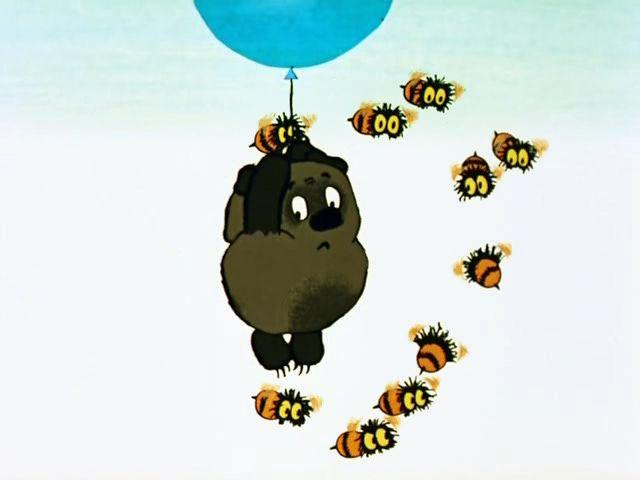
\includegraphics[width=9cm]{images/winnie_kr_4}
\end{figure}



\end{enumerate}


\subsection{Контрольная 4, решения}

\begin{enumerate}

	\item[4.] $H_0: p_{\text{c}} = \frac{1}{7}, p_{\text{л}} = \frac{2}{7}, p_{\text{к}} = \frac{4}{7}$

	$Q = \sum_{i=1}^{s=3} \frac{(\nu_i - np_i)^2}{np_i} \sim \chi^2_{s-k-1} = \chi^2_2$

	$Q_{obs} = \frac{\left(10-70\frac{1}{7}\right)^2}{70\frac{1}{7}} + \frac{\left(1-70\frac{2}{7}\right)^2}{70\frac{2}{7}} + \frac{\left(39-70\frac{4}{7}\right)^2}{70\frac{4}{7}} = 18.075$

	$Q_{crit} = 5.99$, $Q_{crit} < Q_{obs} \Rightarrow$ гипотеза отвергается

	\item[5.] $LR \sim \chi^2_1$, так как основная гипотеза содержит одно уравнение

	$L(x, \lambda) = \prod_{i=1}^{n=50} \lambda e^{-\lambda x} = \lambda^{50} e^{-\lambda \sum_{i=1}^{n=50} x_i}$

	$\ln L (x, \lambda) = 50\ln\lambda - \lambda \sum_{i=1}^{n=50} x_i \to \max_\lambda$

	$\frac{\partial \ln L}{\partial \lambda} = \frac{50}{\lambda} - \sum_{i=1}^{n=50} x_i \mid_{\lambda=\hat{\lambda}} = 0 \Rightarrow \hat{\lambda}_{ML} = \frac{1}{\overline{X}} = \frac{10}{11}$

	При верной $H_0:  \lambda=1$, тогда $\ln L (\lambda=1) = 50 \ln 1 - 1 \cdot 1.1 \cdot 50 = -55$

	При верной $H_1: \lambda=\lambda_{ML}$, тогда $\ln L \left(\lambda=\frac{10}{11}\right) = 50 \ln \frac{10}{11} - \frac{10}{11} \cdot 50 \cdot 1.1 = -54.77$

	$LR_{obs} = 2(\ln L (H_1) - \ln(H_0)) = 2(-54.77- (-55)) = 0.46$

	$LR_{crit} = 2.71$, $LR_{crit} > LR_{obs} \Rightarrow$ оснований отвергать $H_0$ нет

	\item[6.]  Будем проверять гипотезы на уровне значимости $0.05$
		\begin{enumerate}
			\item $\hat{\sigma}^2_{\text{в}} = 484$, $\hat{\sigma}^2_{\text{р}} = 400$

				$\frac{\hat{\sigma}^2_{\text{в}} }{\hat{\sigma}^2_{\text{р}}} \sim F_{21-1 , 19-1}$

				$F_{obs} = \frac{484}{400} = 1.21$, $F_{crit, left} = 0.4$, $F_{crit, right} = 2.6  \Rightarrow$ оснований отвергать $H_0$ нет

			\item $\hat{\sigma}_0^2 = \frac{22\cdot (21-1) + 20 \cdot (19-1)}{21 + 19 - 2} \approx 21$

			$t_{obs} = \frac{78-67}{\sqrt{21} \sqrt{\frac{1}{21}+ \frac{1}{21}}} \approx 7.8 $

			$t_{crit}  \sim t_{21+19-2} = t_{38}$, $t_{crit} = \pm 2.02 \Rightarrow$ гипотеза отвергается
		\end{enumerate}

	\item[7.] $\gamma = \sum_{i=1}^s \sum_{j=1}^m \frac{\left(n_{ij} - \frac{n_{i\cdot}n_{\cdot j}}{n}\right)^2}{\frac{n_{i\cdot}n_{\cdot j}}{n}} \sim \chi^2_{(s-1)(m-1)}$

	$\gamma_{obs} = \frac{\left(12-\frac{44\cdot48}{100}\right)^2}{\frac{44\cdot48}{100}} + \frac{\left(36-\frac{56\cdot48}{100}\right)^2}{\frac{56\cdot48}{100}} + \frac{\left(32-\frac{44\cdot52}{100}\right)^2}{\frac{44\cdot52}{100}} + \frac{\left(20-\frac{50\cdot52}{100}\right)^2}{\frac{50\cdot52}{100}} \approx 12$

	$\gamma_{criit} = 3.84 \Rightarrow$  гипотеза отвергается

\end{enumerate}


\subsection{Экзамен, 20.06.2016}

\element{prob_one_sample}{ % в фигурных скобках название группы вопросов
 \AMCcompleteMulti
  \begin{questionmult}{1} % тип вопроса (questionmult --- множественный выбор) и в фигурных --- номер вопроса
  Случайные величины $X$ и $Y$ распределены нормально. Для тестирования гипотезы о равенстве дисперсий выбирается $m$ наблюдений случайной величины $X$ и $n$ наблюдений случайной величины $Y$. Какое распределение может иметь статистика, используемая в данном случае?
 \begin{multicols}{3} % располагаем ответы в 3 колонки
   \begin{choices} % опция [o] не рандомизирует порядок ответов
      \correctchoice{$F_{m-1,n-1}$}
      \wrongchoice{$F_{m+1,n+1}$}
      \wrongchoice{$F_{m,n}$}
      \wrongchoice{$t_{m+n-2}$}
      \wrongchoice{$t_{m+n-1}$}
      \end{choices}
  \end{multicols}
  \end{questionmult}
}

\element{prob_one_sample}{ % в фигурных скобках название группы вопросов
 \AMCcompleteMulti
  \begin{questionmult}{2} % тип вопроса (questionmult --- множественный выбор) и в фигурных --- номер вопроса
  Требуется проверить гипотезу о равенстве математических ожиданий в двух нормальных выборках размером $m$ и $n$. Если дисперсии неизвестны, но равны, то тестовая статистика имеет распределение
 \begin{multicols}{3} % располагаем ответы в 3 колонки
   \begin{choices} % опция [o] не рандомизирует порядок ответов
      \correctchoice{$t_{m+n-2}$}
      \wrongchoice{$F_{m+1,n+1}$}
      \wrongchoice{$F_{m,n}$}
      \wrongchoice{$F_{m-1,n-1}$}
      \wrongchoice{$t_{m+n-1}$}
      \end{choices}
  \end{multicols}
  \end{questionmult}
}


\element{prob_one_sample}{ % в фигурных скобках название группы вопросов
 \AMCcompleteMulti
  \begin{questionmult}{3} % тип вопроса (questionmult --- множественный выбор) и в фигурных --- номер вопроса
  Требуется проверить гипотезу о равенстве дисперсий по двум нормальным выборкам размером $20$ и $16$ наблюдений. Несмещённая оценка дисперсии по первой выборке составила $60$, по второй — $90$. Тестовая статистика может быть равна
 \begin{multicols}{3} % располагаем ответы в 3 колонки
   \begin{choices} % опция [o] не рандомизирует порядок ответов
      \correctchoice{$1.5$}
      \wrongchoice{$1$}
      \wrongchoice{$1.224$}
      \wrongchoice{$2$}
      \wrongchoice{$4$}
      \end{choices}
  \end{multicols}
  \end{questionmult}
}


\element{prob_one_sample}{ % в фигурных скобках название группы вопросов
 \AMCcompleteMulti
  \begin{questionmult}{4} % тип вопроса (questionmult --- множественный выбор) и в фигурных --- номер вопроса
  Требуется проверить гипотезу о равенстве математических ожиданий по двум нормальным выборкам размером $20$ и $16$ наблюдений. Истинные дисперсии по обеим выборкам известны, совпадают и равны $16$. Разница выборочных средних равна $1$. Тестовая статистика может быть равна
 \begin{multicols}{3} % располагаем ответы в 3 колонки
   \begin{choices} % опция [o] не рандомизирует порядок ответов
      \wrongchoice{$1.5$}
      \wrongchoice{$1$}
      \wrongchoice{$1.224$}
      \wrongchoice{$2$}
      \wrongchoice{$4$}
      \end{choices}
  \end{multicols}
  \end{questionmult}
}


\element{prob_one_sample}{ % в фигурных скобках название группы вопросов
 \AMCcompleteMulti
  \begin{questionmult}{5} % тип вопроса (questionmult --- множественный выбор) и в фигурных --- номер вопроса
  При проверке гипотезе о равенстве математических ожиданий в двух нормальных выборках размеров $m$ и $n$ при известных, но не равных дисперсиях, тестовая статистика имеет распределение
 \begin{multicols}{3} % располагаем ответы в 3 колонки
   \begin{choices} % опция [o] не рандомизирует порядок ответов
      \correctchoice{$N(0;1)$}
      \wrongchoice{$F_{m-1,n-1}$}
      \wrongchoice{$F_{m}$}
      \wrongchoice{$t_{m+n-2}$}
      \wrongchoice{$t_{m+n-1}$}
      \end{choices}
  \end{multicols}
  \end{questionmult}
}


\element{prob_one_sample}{ % в фигурных скобках название группы вопросов
 \AMCcompleteMulti
  \begin{questionmult}{6} % тип вопроса (questionmult --- множественный выбор) и в фигурных --- номер вопроса
  При проверке гипотезы о равенстве долей используется следующее распределение
 \begin{multicols}{3} % располагаем ответы в 3 колонки
   \begin{choices} % опция [o] не рандомизирует порядок ответов
      \correctchoice{$N(0;1)$}
      \wrongchoice{$F_{m-1,n-1}$}
      \wrongchoice{$F_{m, n}$}
      \wrongchoice{$t_{m+n-2}$}
      \wrongchoice{$t_{m+n-1}$}
      \end{choices}
  \end{multicols}
  \end{questionmult}
}


\element{prob_one_sample_rejected}{ % в фигурных скобках название группы вопросов
 \AMCcompleteMulti
  \begin{questionmult}{7} % тип вопроса (questionmult --- множественный выбор) и в фигурных --- номер вопроса
   Есть две нормально распределённых выборки размером $20$ и $16$ наблюдений. Истинные дисперсии по обеим выборкам неизвестны и равны. Выборочные средние по обеим выборкам совпадают. Гипотеза о равенстве математических ожиданий
 %\begin{multicols}{3} % располагаем ответы в 3 колонки
   \begin{choices} % опция [o] не рандомизирует порядок ответов
      \correctchoice{не отвергается на любом разумном уровне значимости}
      \wrongchoice{отвергается на любом разумном уровне значимости}
      \wrongchoice{не отвергается на 5\%-ом и отвергается на 1\%-ом уровне значимости}
      \wrongchoice{не отвергается на 1\%-ом и отвергается на 5\%-ом уровне значимости}
      \wrongchoice{Гипотезу невозможно проверить}
      \end{choices}
  %\end{multicols}
  \end{questionmult}
}


\element{prob_one_sample}{ % в фигурных скобках название группы вопросов
 \AMCcompleteMulti
  \begin{questionmult}{8} % тип вопроса (questionmult --- множественный выбор) и в фигурных --- номер вопроса
  Для проверки гипотезы о равенстве долей в двух выборках  могут использоваться следующие распределения
 \begin{multicols}{3} % располагаем ответы в 3 колонки
   \begin{choices} % опция [o] не рандомизирует порядок ответов
      \wrongchoice{только $N(0;1)$}
      \correctchoice{$N(0;1)$ и $\chi^2_1$}
      \wrongchoice{только $\chi^2_1$}
      \wrongchoice{$N(0;1)$ и $F_{m,n}$}
      \wrongchoice{только $F_{m,n}$}
      \end{choices}
  \end{multicols}
  \end{questionmult}
}

\element{prob_one_sample}{ % в фигурных скобках название группы вопросов
 \AMCcompleteMulti
  \begin{questionmult}{9} % тип вопроса (questionmult --- множественный выбор) и в фигурных --- номер вопроса
  Доля успехов в первой выборке равна $0.55$, доля успехов во второй выборке --- $0.4$. Количество наблюдений в выборках равно $40$ и $20$ соответственно. Тестовая статистика для проверки гипотезы о равенстве долей может быть равна
 \begin{multicols}{3} % располагаем ответы в 3 колонки
   \begin{choices} % опция [o] не рандомизирует порядок ответов
      \correctchoice{$1.1$}
      \wrongchoice{$2.2$}
      \wrongchoice{$1.2$}
      \wrongchoice{$2.4$}
      \wrongchoice{$0.9$}
      \end{choices}
  \end{multicols}
  \end{questionmult}
}

\element{prob_one_sample}{ % в фигурных скобках название группы вопросов
 \AMCcompleteMulti
  \begin{questionmult}{10} % тип вопроса (questionmult --- множественный выбор) и в фигурных --- номер вопроса
  Доля успехов в первой выборке равна $0.8$, доля успехов во второй выборке --- $0.3$. Количество наблюдений в выборках $40$ и $20$ соответственно. Гипотеза о равенстве долей
 %\begin{multicols}{3} % располагаем ответы в 3 колонки
   \begin{choices} % опция [o] не рандомизирует порядок ответов
     \correctchoice{отвергается на любом разумном уровне значимости}
     \wrongchoice{не отвергается на любом разумном уровне значимости}
     \wrongchoice{не отвергается на 5\%-ом и отвергается на 1\%-ом уровне значимости}
     \wrongchoice{не отвергается на 1\%-ом и отвергается на 5\%-ом уровне значимости}
     \wrongchoice{Гипотезу невозможно проверить}
      \end{choices}
  %\end{multicols}
  \end{questionmult}
}























\element{prob_two_samples}{ % в фигурных скобках название группы вопросов
 \AMCcompleteMulti
  \begin{questionmult}{2} % тип вопроса (questionmult --- множественный выбор) и в фигурных --- номер вопроса
  Для выборки $X_1,\ldots,X_n$, имеющей нормальное распределение, проверяется гипотеза $H_0: \sigma^2=\sigma_0^2$ против $H_a: \sigma^2 > \sigma_0^2$. Критическая область имеет вид
 %\begin{multicols}{3} % располагаем ответы в 3 колонки
   \begin{choices} % опция [o] не рандомизирует порядок ответов
      \correctchoice{$(A,+\infty)$, где $A$ таково, что $\P(\chi^2_{n-1} < A) =1-\alpha$}
      \wrongchoice{$(A,+\infty)$, где $A$ таково, что $\P(\chi^2_{n-1} < A)  =\alpha$}
      \wrongchoice{$(0,A)$, где $A$ таково, что $\P(\chi^2_{n-1} < A)  =1-\alpha$}
      \wrongchoice{$(-\infty,A)$, где $A$ таково, что $\P(\chi^2_{n-1} < A)  =1-\alpha$}
      \wrongchoice{ $(0,A)$, где $A$ таково, что $\P(\chi^2_{n-1} < A)  =\alpha$}
      \end{choices}
  %\end{multicols}
  \end{questionmult}
}


% \element{prob_two_samples_rejected}{ % в фигурных скобках название группы вопросов
%  \AMCcompleteMulti
%   \begin{questionmult}{3} % тип вопроса (questionmult --- множественный выбор) и в фигурных --- номер вопроса
%   Для выборки $X_1,\ldots,X_n$, имеющей нормальное распределение, проверяется гипотеза $H_0: \sigma^2=\sigma_0^2$ против $H_a: \sigma^2 < \sigma_0^2$. Критическая область имеет вид
%  %\begin{multicols}{3} % располагаем ответы в 3 колонки
%    \begin{choices} % опция [o] не рандомизирует порядок ответов
%       \correctchoice{$(0,A)$, где $A$ таково, что $F_{\chi^2_{n-1}} (A) =\alpha$}
%       \wrongchoice{$(0,A)$, где $A$ таково, что $F_{\chi^2_{n-1}} (A) =1-\alpha$}
%       \wrongchoice{$(-\infty,A)$, где $A$ таково, что $F_{\chi^2_{n-1}} (A) =\alpha$}
%       \wrongchoice{ $(A,+\infty)$, где $A$ таково, что $F_{\chi^2_{n-1}} (A) =1-\alpha$}
%       \end{choices}
%   %\end{multicols}
%   \end{questionmult}
% }


\element{prob_two_samples}{ % в фигурных скобках название группы вопросов
 \AMCcompleteMulti
  \begin{questionmult}{4} % тип вопроса (questionmult --- множественный выбор) и в фигурных --- номер вопроса
  При подбрасывании игральной кости 600 раз шестерка выпала 105 раз. Гипотеза о том, что кость правильная
 %\begin{multicols}{3} % располагаем ответы в 3 колонки
   \begin{choices} % опция [o] не рандомизирует порядок ответов
      \correctchoice{не отвергается при любом разумном значении $\alpha$}
      \wrongchoice{отвергается при любом разумном значении $\alpha$}
      \wrongchoice{отвергается при $\alpha = 0.05$, не отвергается при $\alpha = 0.01$}
      \wrongchoice{отвергается при $\alpha = 0.01$, не отвергается при $\alpha = 0.05$}
      \wrongchoice{Гипотезу невозможно проверить}
      \end{choices}
  %\end{multicols}
  \end{questionmult}
}


\element{prob_two_samples}{ % в фигурных скобках название группы вопросов
 \AMCcompleteMulti
  \begin{questionmult}{5} % тип вопроса (questionmult --- множественный выбор) и в фигурных --- номер вопроса
  Величины $X_1,\ldots,X_n$ --- выборка из нормально распределенной случайной величины с неизвестным математическим ожиданием и известной дисперсией. На уровне значимости $\alpha$ проверяется гипотеза $H_0: \mu = \mu_0$ против $H_a: \mu \neq \mu_0$. Обозначим $\varphi_1$ и $\varphi_2$ вероятности ошибок первого и второго рода соответственно. Между параметрами задачи всегда выполнено соотношение
 \begin{multicols}{3} % располагаем ответы в 3 колонки
   \begin{choices} % опция [o] не рандомизирует порядок ответов
      \correctchoice{$\varphi_1 = \alpha$}
      \wrongchoice{$\varphi_1 = 1 - \alpha$}
      \wrongchoice{$\varphi_2 = \alpha$}
      \wrongchoice{$\varphi_2 = 1 - \alpha$}
      \wrongchoice{$\varphi_1 + \varphi_2 = \alpha$}
      \end{choices}
  \end{multicols}
  \end{questionmult}
}


\element{prob_two_samples}{ % в фигурных скобках название группы вопросов
 \AMCcompleteMulti
  \begin{questionmult}{6} % тип вопроса (questionmult --- множественный выбор) и в фигурных --- номер вопроса
  По случайной выборке из 200 наблюдений было оценено выборочное среднее $\bar{X} = 25$  и несмещённая оценка дисперсии $\hat{\sigma}^2 = 25$. В рамках проверки гипотезы $H_0: \mu = 20$ против $H_a: \mu > 20$ можно сделать вывод, что гипотеза $H_0$
 %\begin{multicols}{3} % располагаем ответы в 3 колонки
   \begin{choices} % опция [o] не рандомизирует порядок ответов
      \correctchoice{отвергается при любом разумном значении $\alpha$}
      \wrongchoice{отвергается при $\alpha = 0.05$, не отвергается при $\alpha = 0.01$}
      \wrongchoice{отвергается при $\alpha = 0.01$, не отвергается при $\alpha = 0.05$}
      \wrongchoice{не отвергается при любом разумном значении $\alpha$}
      \wrongchoice{Гипотезу невозможно проверить}
      \end{choices}
  %\end{multicols}
  \end{questionmult}
}


\element{prob_two_samples}{ % в фигурных скобках название группы вопросов
 \AMCcompleteMulti
  \begin{questionmult}{7} % тип вопроса (questionmult --- множественный выбор) и в фигурных --- номер вопроса
   По выборке $X_1,\ldots, X_n$ из нормального распределения строятся по стандартным формулам доверительные интервалы для математического ожидания. Получен интервал $(a_1,a_2)$ при известной дисперсии и интервал $(b_1,b_2)$ при неизвестной дисперсии. Всегда справедливы следующие соотношения:
 \begin{multicols}{2} % располагаем ответы в 3 колонки
   \begin{choices} % опция [o] не рандомизирует порядок ответов
      \correctchoice{$|a_1-b_1| = |a_2-b_2|$}
      \wrongchoice{$a_2 - a_1 < b_2 - b_1$}
      \wrongchoice{$a_2 - a_1 > b_2 - b_1$}
      \wrongchoice{$a_1<0,b_1<0,a_2>0,b_2>0$}
      \wrongchoice{$a_1>0,b_1>0,a_2>0,b_2>0$}
      \end{choices}
  \end{multicols}
  \end{questionmult}
}


\element{prob_two_samples}{ % в фигурных скобках название группы вопросов
 \AMCcompleteMulti
  \begin{questionmult}{8} % тип вопроса (questionmult --- множественный выбор) и в фигурных --- номер вопроса
  Величины $X_1,\ldots,X_n$ --- выборка из нормального распределения.  Статистика $U=\frac{5-\bar{X}}{5/\sqrt{n}}$ применима для проверки
 %\begin{multicols}{3} % располагаем ответы в 3 колонки
   \begin{choices} % опция [o] не рандомизирует порядок ответов
      \wrongchoice{гипотезы $H_0: \mu = 5$ при известной дисперсии, равной 5, при любых $n$}
      \correctchoice{гипотезы $H_0: \mu = 5$ при известной дисперсии, равной 25, при любых $n$}
      \wrongchoice{гипотезы $H_0: \mu = 5$ при известной дисперсии, равной 5, при больших $n$}
      \wrongchoice{гипотезы $H_0: \mu = 5$ при известной дисперсии, равной 25, только при больших $n$}
      \wrongchoice{гипотезы $H_0: \sigma = 5$}
      \end{choices}
  %\end{multicols}
  \end{questionmult}
}

\element{prob_two_samples}{ % в фигурных скобках название группы вопросов
 \AMCcompleteMulti
  \begin{questionmult}{9} % тип вопроса (questionmult --- множественный выбор) и в фигурных --- номер вопроса
Выборочная доля успехов в некотором испытании составляет $0.3$. Исследователь Ромео хочет, чтобы длина двустороннего 95\%-го доверительного интервала для истинной доли не превышала $0.1$. Количество наблюдений, необходимых для этого, примерно равно
 \begin{multicols}{3} % располагаем ответы в 3 колонки
   \begin{choices} % опция [o] не рандомизирует порядок ответов
      \correctchoice{$322$}
      \wrongchoice{$161$}
      \wrongchoice{$113$}
      \wrongchoice{$225$}
      \wrongchoice{$81$}
      \end{choices}
  \end{multicols}
  \end{questionmult}
}

\element{prob_two_samples}{ % в фигурных скобках название группы вопросов
 \AMCcompleteMulti
  \begin{questionmult}{10} % тип вопроса (questionmult --- множественный выбор) и в фигурных --- номер вопроса
  Пусть $X_1,\ldots,X_n$ --- выборка из нормального распределения с известной дисперсией $\sigma^2$. Пусть $U = \frac{\bar{X}-\mu_0}{\sigma/\sqrt{n}}$. Величина $U^2$ имеет распределение
 \begin{multicols}{3} % располагаем ответы в 3 колонки
   \begin{choices} % опция [o] не рандомизирует порядок ответов
     \correctchoice{$\chi^2_1$}
     \wrongchoice{$\chi^2_{n-1}$}
     \wrongchoice{$t_1$}
     \wrongchoice{$t_{n-1}$}
     \wrongchoice{$F_{1,n-1}$}
      \end{choices}
  \end{multicols}
  \end{questionmult}
}
























\element{prob_sample_char}{ % в фигурных скобках название группы вопросов
 \AMCcompleteMulti
  \begin{questionmult}{1} % тип вопроса (questionmult --- множественный выбор) и в фигурных --- номер вопроса
  Дана реализация выборки: 3, 1, 2. Выборочный начальный момент первого порядка равен
 \begin{multicols}{3} % располагаем ответы в 3 колонки
   \begin{choices} % опция [o] не рандомизирует порядок ответов
      \correctchoice{2}
      \wrongchoice{1}
      \wrongchoice{0}
      \wrongchoice{3}
      \wrongchoice{14/3}
      \end{choices}
  \end{multicols}
  \end{questionmult}
}

\element{prob_sample_char}{ % в фигурных скобках название группы вопросов
 \AMCcompleteMulti
  \begin{questionmult}{2} % тип вопроса (questionmult --- множественный выбор) и в фигурных --- номер вопроса
  Дана реализация выборки: 3, 1, 2. Несмещённая оценка дисперсии равна
 \begin{multicols}{3} % располагаем ответы в 3 колонки
   \begin{choices} % опция [o] не рандомизирует порядок ответов
      \correctchoice{1}
      \wrongchoice{1/2}
      \wrongchoice{1/3}
      \wrongchoice{2/3}
      \wrongchoice{2}
      \end{choices}
  \end{multicols}
  \end{questionmult}
}


\element{prob_sample_char}{ % в фигурных скобках название группы вопросов
 \AMCnoCompleteMulti
  \begin{questionmult}{3} % тип вопроса (questionmult --- множественный выбор) и в фигурных --- номер вопроса
  Выберите НЕВЕРНОЕ утверждение про эмпирическую функцию распределения $F_n(x)$
 %\begin{multicols}{3} % располагаем ответы в 3 колонки
   \begin{choices} % опция [o] не рандомизирует порядок ответов
      \correctchoice{$F_n(x)$ является невозрастающей функцией}
      %\wrongchoice{$F_n(x)$ является состоятельной оценкой функции распределения $F(x)$}
      \wrongchoice{$F_n(x)$ имеет разрыв в каждой точке вариационного ряда}
      \wrongchoice{$F_n(x)$ асимптотически нормальна}
      \wrongchoice{$\E(F_n(x))=F(x)$}
      \wrongchoice{$\Var(F_n(x))=F(x)(1-F(x))/n$}
      \end{choices}
  %\end{multicols}
  \end{questionmult}
}


\element{prob_sample_char}{ % в фигурных скобках название группы вопросов
 \AMCcompleteMulti
  \begin{questionmult}{4} % тип вопроса (questionmult --- множественный выбор) и в фигурных --- номер вопроса
 Юрий Петров утверждает, что обычно посещает половину занятий по Статистике. За последние полгода из 36 занятий он не посетил ни одного. Вычислите значение критерия хи-квадрат Пирсона для гипотезы, что утверждение Юрия Петрова истинно и укажите число степеней свободы
 \begin{multicols}{3} % располагаем ответы в 3 колонки
   \begin{choices} % опция [o] не рандомизирует порядок ответов
      \correctchoice{$\chi^2 = 36$, $df=1$}
      \wrongchoice{$\chi^2 = 2$, $df=2$}
      \wrongchoice{$\chi^2 = 14$, $df=1$}
      \wrongchoice{$\chi^2 = 20$, $df=2$}
      \wrongchoice{$\chi^2 = 24$, $df=1$}
      \end{choices}
  \end{multicols}
  \end{questionmult}
}


\element{prob_sample_char}{ % в фигурных скобках название группы вопросов
 \AMCcompleteMulti
  \begin{questionmult}{5} % тип вопроса (questionmult --- множественный выбор) и в фигурных --- номер вопроса
  Производитель фломастеров попросил трёх человек оценить два вида фломастеров: «Лесенка» и «Erich Krause» по 10-балльной шкале:

\begin{center}
\begin{tabular}{lrrr} \toprule
 & Пафнутий & Андрей & Карл \\
\midrule
Лесенка & 9 & 7 & 6 \\
Erich Krause & 8 & 9 & 7 \\
\bottomrule
\end{tabular}
\end{center}

\textbf{Точное} $P$-значение ($P$-value) статистики теста знаков равно

 \begin{multicols}{3} % располагаем ответы в 3 колонки
   \begin{choices} % опция [o] не рандомизирует порядок ответов
      \correctchoice{1/2}
      \wrongchoice{1/8}
      \wrongchoice{1/3}
      \wrongchoice{3/8}
      \wrongchoice{2/3}
      \end{choices}
  \end{multicols}
  \end{questionmult}
}


\element{prob_sample_char}{ % в фигурных скобках название группы вопросов
 \AMCcompleteMulti
  \begin{questionmult}{6} % тип вопроса (questionmult --- множественный выбор) и в фигурных --- номер вопроса
  Производитель фломастеров попросил трёх человек оценить два вида фломастеров: «Лесенка» и «Erich Krause» по 10-балльной шкале:

\begin{center}
\begin{tabular}{lrrr} \toprule
 & Пафнутий  & Андрей & Карл \\
\midrule
Лесенка & 9 & 7 & 6 \\
Erich Krause & 8 & 9 & 7 \\
\bottomrule
\end{tabular}
\end{center}

Вычислите модуль значения статистики теста знаков. \textbf{Используя нормальную аппроксимацию}, проверьте на уровне значимости 0.1 гипотезу о том, что фломастеры имеют одинаковое качество.

 \begin{multicols}{3} % располагаем ответы в 3 колонки
   \begin{choices} % опция [o] не рандомизирует порядок ответов
      \correctchoice{0.58, $H_0$ не отвергается}
      \wrongchoice{0.58, $H_0$ отвергается}
      \wrongchoice{0.43, $H_0$ не отвергается}
      \wrongchoice{1.65, $H_0$ отвергается}
      \wrongchoice{1.96, $H_0$ отвергается}
      \end{choices}
  \end{multicols}
  \end{questionmult}
}


\element{prob_sample_char}{ % в фигурных скобках название группы вопросов
 \AMCcompleteMulti
  \begin{questionmult}{7} % тип вопроса (questionmult --- множественный выбор) и в фигурных --- номер вопроса
   Кузнец Вакула в течение 100 лет ведет статистику о прилете аистов и рождении младенцев на хуторе близ Диканьки. У него получилась следующая таблица сопряженности

\begin{center}
\begin{tabular}{lrr} \toprule
& Аисты прилетали  & Аисты не прилетали \\
\midrule
Появлялся младенец & 30 & 10 \\
Не появлялся младенец & 30 & 30 \\
\bottomrule
\end{tabular}
\end{center}

Укажите число степеней свободы статистики Пирсона и на уровне значимости 5\% определите, зависит ли появление младенца от прилета аистов

 \begin{multicols}{3} % располагаем ответы в 3 колонки
   \begin{choices} % опция [o] не рандомизирует порядок ответов
      \correctchoice{$df=1$, зависит}
      \wrongchoice{$df=1$, не зависит}
      \wrongchoice{$df=3$, зависит}
      \wrongchoice{$df=4$, зависит}
      \wrongchoice{$df=2$, зависит}
      \end{choices}
  \end{multicols}
  \end{questionmult}
}



\element{prob_sample_char}{ % в фигурных скобках название группы вопросов
 \AMCcompleteMulti
  \begin{questionmult}{8} % тип вопроса (questionmult --- множественный выбор) и в фигурных --- номер вопроса
  В коробке 50 купюр пяти различных номиналов. Случайным образом достаются две купюры. Номиналы вынимаемых купюр
 \begin{multicols}{2} % располагаем ответы в 3 колонки
   \begin{choices} % опция [o] не рандомизирует порядок ответов
   \correctchoice{отрицательно коррелированы}
   \wrongchoice{положительно коррелированы}
    \wrongchoice{не коррелированы и не зависимы}
    \wrongchoice{не коррелированы, но зависимы}
    \wrongchoice{положительно коррелированы, но не зависимы}
      \end{choices}
  \end{multicols}
  \end{questionmult}
}



\element{prob_sample_char}{ % в фигурных скобках название группы вопросов
 \AMCcompleteMulti
  \begin{questionmult}{9} % тип вопроса (questionmult --- множественный выбор) и в фигурных --- номер вопроса
Экзамен принимают два преподавателя: Злой и Добрый. Они поставили следующие оценки:

\begin{center}
\begin{tabular}{lrrrrr} \toprule
Злой   & 2 & 3 & 10 & 8 & 3 \\
Добрый & 6 & 4 & 7  & 8 & \\
\bottomrule
\end{tabular}
\end{center}

Значение статистики критерия Вилкоксона о совпадении распределений оценок равно

 \begin{multicols}{3} % располагаем ответы в 3 колонки
   \begin{choices} % опция [o] не рандомизирует порядок ответов
     \correctchoice{22.5}
     \wrongchoice{7.5}
     \wrongchoice{19}
     \wrongchoice{20}
     \wrongchoice{20.5}
      \end{choices}
  \end{multicols}
  \end{questionmult}
}



\element{prob_sample_char}{ % в фигурных скобках название группы вопросов
 \AMCcompleteMulti
  \begin{questionmult}{10} % тип вопроса (questionmult --- множественный выбор) и в фигурных --- номер вопроса
Датчик случайных чисел выдал два значения псевдослучайных чисел: $0.5$ и $0.9$. Вычислите значение критерия Колмогорова и проверьте гипотезу о соответствии распределения равномерному на уровне значимости $0.1$. Критическое значение статистики Колмогорова для уровня значимости $0.1$ и двух наблюдений равно $0.776$.
 \begin{multicols}{3} % располагаем ответы в 3 колонки
   \begin{choices} % опция [o] не рандомизирует порядок ответов
      \correctchoice{$0.5$, $H_0$ не отвергается}
      \wrongchoice{$1.4$, $H_0$ отвергается}
      \wrongchoice{$0.9$, $H_0$ отвергается}
      \wrongchoice{$0.9$, $H_0$ не отвергается}
      \wrongchoice{$0.4$, $H_0$ не отвергается}
      \end{choices}
  \end{multicols}
  \end{questionmult}
}


























\element{prob_ml_mm}{ % в фигурных скобках название группы вопросов
 \AMCnoCompleteMulti
  \begin{questionmult}{1} % тип вопроса (questionmult --- множественный выбор) и в фигурных --- номер вопроса
  Выберите НЕВЕРНОЕ утверждение про метод максимального правдоподобия (ММП):
 %\begin{multicols}{3} % располагаем ответы в 3 колонки
   \begin{choices} % опция [o] не рандомизирует порядок ответов
      \correctchoice{Оценки ММП асимтотически нормальны $\cN(0;1)$}
      \wrongchoice{ММП применим для зависимых случайных величин}
      \wrongchoice{ММП применим для оценивания двух и более параметров}
      \wrongchoice{При выполнении технических предпосылок оценки ММП состоятельны}
      \wrongchoice{ММП оценки не всегда совпадают с оценками метода моментов}
      \end{choices}
  %\end{multicols}
  \end{questionmult}
}

\element{prob_ml_mm}{ % в фигурных скобках название группы вопросов
 \AMCcompleteMulti
  \begin{questionmult}{2} % тип вопроса (questionmult --- множественный выбор) и в фигурных --- номер вопроса
  Если величина $\hat\theta$ имеет нормальное распределение $\cN(2;0.01^2)$, то, согласно дельта-методу, $\hat\theta^2$ имеет примерно нормальное распределение
 \begin{multicols}{3} % располагаем ответы в 3 колонки
   \begin{choices} % опция [o] не рандомизирует порядок ответов
      \correctchoice{$\cN(4;16\cdot 0.01^2)$}
      \wrongchoice{$\cN(4;4\cdot 0.01^2)$}
      \wrongchoice{$\cN(2;4\cdot 0.01^2)$}
      \wrongchoice{$\cN(4;8\cdot 0.01^2)$}
      \wrongchoice{$\cN(4;2\cdot 0.01^2)$}
      \end{choices}
  \end{multicols}
  \end{questionmult}
}


\element{prob_ml_mm}{ % в фигурных скобках название группы вопросов
 \AMCcompleteMulti
  \begin{questionmult}{3} % тип вопроса (questionmult --- множественный выбор) и в фигурных --- номер вопроса
  Случайные величины $X_1$, $X_2$ и $X_3$ независимы и одинаково распределены,

\begin{center}
  \begin{tabular}{lrr} \toprule
  $X_i$ & 3 & 5 \\
  \midrule
  $\P(\cdot)$ & $p$ & $1-p$ \\
  \bottomrule
  \end{tabular}
\end{center}

  Имеется выборка из трёх наблюдений: $X_1=5$, $X_2=3$, $X_3=5$. Оценка неизвестного $p$, полученная методом максимального правдоподобия, равна:


 \begin{multicols}{3} % располагаем ответы в 3 колонки
   \begin{choices} % опция [o] не рандомизирует порядок ответов
      \correctchoice{$1/3$}
      \wrongchoice{$1/2$}
      \wrongchoice{$1/4$}
      \wrongchoice{$2/3$}
      \wrongchoice{Метод неприменим}
      \end{choices}
  \end{multicols}
  \end{questionmult}
}


\element{prob_ml_mm}{ % в фигурных скобках название группы вопросов
 \AMCcompleteMulti
  \begin{questionmult}{4} % тип вопроса (questionmult --- множественный выбор) и в фигурных --- номер вопроса
    Случайные величины $X_1$, $X_2$ и $X_3$ независимы и одинаково распределены,

\begin{center}
    \begin{tabular}{lrr} \toprule
    $X_i$ & 3 & 5 \\
    \midrule
    $\P(\cdot)$ & $p$ & $1-p$ \\
    \bottomrule
    \end{tabular}
\end{center}

    По выборке оказалось, что $\bar X = 4.5$. Оценка неизвестного $p$, полученная методом моментов, равна:


   \begin{multicols}{3} % располагаем ответы в 3 колонки
     \begin{choices} % опция [o] не рандомизирует порядок ответов
        \correctchoice{$1/4$}
        \wrongchoice{$1/2$}
        \wrongchoice{$1/3$}
        \wrongchoice{$2/3$}
        \wrongchoice{Метод неприменим}
      \end{choices}
  \end{multicols}
  \end{questionmult}
}

\element{prob_ml_mm}{ % в фигурных скобках название группы вопросов
 \AMCcompleteMulti
  \begin{questionmult}{5} % тип вопроса (questionmult --- множественный выбор) и в фигурных --- номер вопроса
  Величины $X_1$, $X_2$, \ldots, $X_{2016}$ независимы и одинаково распределены, $\cN(\mu ; 42)$. Оказалось, что $\bar X =  -23$. Про оценки метода моментов, $\hat \mu_{MM}$, и метода максимального правдоподобия, $\hat \mu_{ML}$, можно утверждать, что

 \begin{multicols}{3} % располагаем ответы в 3 колонки
   \begin{choices} % опция [o] не рандомизирует порядок ответов
      \correctchoice{$\hat \mu_{ML} = -23$, $\hat\mu_{MM} = -23$}
      \wrongchoice{$\hat \mu_{ML} > -23$, $\hat\mu_{MM} = -23$}
      \wrongchoice{$\hat \mu_{ML} = -23$, $\hat\mu_{MM} > -23$}
      \wrongchoice{$\hat \mu_{ML} < -23$, $\hat\mu_{MM} = -23$}
      \wrongchoice{$\hat \mu_{ML} = -23$, $\hat\mu_{MM} < -23$}
      \end{choices}
  \end{multicols}
  \end{questionmult}
}


\element{prob_ml_mm}{ % в фигурных скобках название группы вопросов
 \AMCnoCompleteMulti
  \begin{questionmult}{6} % тип вопроса (questionmult --- множественный выбор) и в фигурных --- номер вопроса
 Выберите НЕВЕРНОЕ утверждение про логарифмическую функцию правдоподобия $\ell(\theta)$

 %\begin{multicols}{3} % располагаем ответы в 3 колонки
   \begin{choices} % опция [o] не рандомизирует порядок ответов
      \correctchoice{Функция $\ell(\theta)$ имеет максимум при $\theta=0$}
      \wrongchoice{Функция $\ell(\theta)$ может принимать отрицательные значения}
      \wrongchoice{Функция $\ell(\theta)$ может принимать положительные значения}
      \wrongchoice{Функция $\ell(\theta)$ может принимать значения больше единицы}
      \wrongchoice{Функция $\ell(\theta)$ может иметь несколько экстремумов}
      \end{choices}
  %\end{multicols}
  \end{questionmult}
}


\element{prob_ml_mm}{ % в фигурных скобках название группы вопросов
 \AMCcompleteMulti
  \begin{questionmult}{7} % тип вопроса (questionmult --- множественный выбор) и в фигурных --- номер вопроса
Величины $X_1$, \ldots, $X_n$ независимы и одинаково распределены, $\E(X_1^2)=2\theta + 4$. По выборке из 100 наблюдений оказалось, что $\sum_{i=1}^{100} X_i^2 = 200$. Оценка метода момента, $\hat\theta_{MM}$, равна

 \begin{multicols}{3} % располагаем ответы в 3 колонки
   \begin{choices} % опция [o] не рандомизирует порядок ответов
      \correctchoice{-1}
      \wrongchoice{1}
      \wrongchoice{0}
      \wrongchoice{2}
      \wrongchoice{Метод неприменим}
      \end{choices}
  \end{multicols}
  \end{questionmult}
}



\element{prob_ml_mm}{ % в фигурных скобках название группы вопросов
 \AMCcompleteMulti
  \begin{questionmult}{8} % тип вопроса (questionmult --- множественный выбор) и в фигурных --- номер вопроса
По выборке из 100 наблюдений построена оценка метода максимального правдоподобия, $\hat \theta_{ML} = 42$. Вторая производная лог-функции правдоподобия равна $\ell''(\hat\theta) = -1$. Ширина 95\%-го доверительного интервала для неизвестного параметра $\theta$ примерно равна
 \begin{multicols}{3} % располагаем ответы в 3 колонки
   \begin{choices} % опция [o] не рандомизирует порядок ответов
   \correctchoice{4}
   \wrongchoice{1}
    \wrongchoice{2}
    \wrongchoice{8}
    \wrongchoice{1/2}
  \end{choices}
  \end{multicols}
  \end{questionmult}
}



\element{prob_ml_mm}{ % в фигурных скобках название группы вопросов
 \AMCcompleteMulti
  \begin{questionmult}{9} % тип вопроса (questionmult --- множественный выбор) и в фигурных --- номер вопроса
  Проверяется гипотеза $H_0$: $\theta = \gamma$ против альтернативной гипотезы $H_a$: $\theta \neq \gamma$, где $\theta$ и $\gamma$ --- два неизвестных параметра. Выберите верное утверждение о распределении статистики отношения правдоподобия, $LR$:

 \begin{multicols}{2} % располагаем ответы в 3 колонки
   \begin{choices} % опция [o] не рандомизирует порядок ответов
     \correctchoice{Если верна $H_0$, то $LR \sim \chi_1^2$}
     \wrongchoice{Если верна $H_a$, то $LR \sim \chi_1^2$}
     \wrongchoice{Если верна $H_a$, то $LR \sim \chi_2^2$}
     \wrongchoice{И при $H_0$, и при $H_a$, $LR \sim \chi_1^2$}
     \wrongchoice{И при $H_0$, и при $H_a$, $LR \sim \chi_2^2$}
      \end{choices}
  \end{multicols}
  \end{questionmult}
}



\element{prob_ml_mm}{ % в фигурных скобках название группы вопросов
 \AMCcompleteMulti
  \begin{questionmult}{10} % тип вопроса (questionmult --- множественный выбор) и в фигурных --- номер вопроса
  По 100 наблюдениям получена оценка метода максимального правдоподобия, $\hat\theta = 20$, также известны значения лог-функции правдоподобия $\ell(20) = -10$ и $\ell(0)= - 50$. С помощью критерия отношения правдоподобия, $LR$, проверьте гипотезу $H_0$: $\theta = 0$ против $H_0$: $\theta \neq 0$ на уровне значимости 5\%.
 \begin{multicols}{2} % располагаем ответы в 3 колонки
   \begin{choices} % опция [o] не рандомизирует порядок ответов
      \correctchoice{$LR = 80$, $H_0$ отвергается }
      \wrongchoice{$LR = 60$, $H_0$ не отвергается}
      \wrongchoice{$LR = 40$, $H_0$ не отвергается}
      \wrongchoice{$LR = 40$, $H_0$  отвергается}
      \wrongchoice{Критерий неприменим}
      \end{choices}
  \end{multicols}
  \end{questionmult}
}



























\element{prob_estimators}{ % в фигурных скобках название группы вопросов
 \AMCcompleteMulti
  \begin{questionmult}{1} % тип вопроса (questionmult --- множественный выбор) и в фигурных --- номер вопроса
Пусть $X = (X_1, \ldots , X_n)$ --- случайная выборка из биномиального распределения $Bi(5, p)$. Известно, что $\P(X = x) =C_n^x p^x(1-p)^{n-x} $. Информация Фишера $I_n(p)$ равна:
 \begin{multicols}{3} % располагаем ответы в 3 колонки
   \begin{choices} % опция [o] не рандомизирует порядок ответов
      \correctchoice{$\frac{5n}{p(1-p)}$}
      \wrongchoice{$\frac{p(1-p)}{5n}$}
      \wrongchoice{$\frac{5p(1-p)}{n}$}
      \wrongchoice{$\frac{n}{5p(1-p)}$}
      \wrongchoice{$\frac{n}{p(1-p)}$}
      \end{choices}
  \end{multicols}
  \end{questionmult}
}

\element{prob_estimators}{ % в фигурных скобках название группы вопросов
 \AMCcompleteMulti
  \begin{questionmult}{2} % тип вопроса (questionmult --- множественный выбор) и в фигурных --- номер вопроса
Пусть $X = (X_1, \ldots , X_n)$ --- случайная выборка из экспоненциального распределения с плотностью
\[
f(x; \theta) =
\begin{cases}
\frac{1}{\theta}\exp(-\frac{x}{\theta}) \text{ при } x \geq 0,  \\
0 \text{ при } x < 0.
\end{cases}
\]
Информация Фишера $I_n(p)$ равна:
 \begin{multicols}{3} % располагаем ответы в 3 колонки
   \begin{choices} % опция [o] не рандомизирует порядок ответов
      \correctchoice{$\frac{n}{\theta^2}$}
      \wrongchoice{$n \theta^2$}
      \wrongchoice{$\frac{\theta^2}{n}$}
      \wrongchoice{$\frac{\theta}{n}$}
      \wrongchoice{$\frac{n}{\theta}$}
      \end{choices}
  \end{multicols}
  \end{questionmult}
}


\element{prob_estimators}{ % в фигурных скобках название группы вопросов
 \AMCcompleteMulti
  \begin{questionmult}{3} % тип вопроса (questionmult --- множественный выбор) и в фигурных --- номер вопроса
Пусть $X = (X_1, \ldots , X_n)$ --- случайная выборка из равномерного на $(0, \theta)$ распределения. При каком значении константы $c$ оценка  $\hat{\theta} = c \bar{X}$ является несмещённой?
 \begin{multicols}{3} % располагаем ответы в 3 колонки
   \begin{choices} % опция [o] не рандомизирует порядок ответов
      \correctchoice{$2$}
      \wrongchoice{$1$}
      \wrongchoice{$\frac{1}{2}$}
      \wrongchoice{$\frac{1}{n}$}
      \wrongchoice{$n$}
      \end{choices}
  \end{multicols}
  \end{questionmult}
}

\element{prob_estimators_rejected}{ % в фигурных скобках название группы вопросов
 \AMCcompleteMulti
  \begin{questionmult}{3} % тип вопроса (questionmult --- множественный выбор) и в фигурных --- номер вопроса
Пусть $X = (X_1, \ldots , X_n)$ --- случайная выборка из биномиального распределения $Bi(5, p)$. При каком значении константы $c$ оценка  $\hat{p} = c \bar{X}$ является несмещённой?
 \begin{multicols}{3} % располагаем ответы в 3 колонки
   \begin{choices} % опция [o] не рандомизирует порядок ответов
      \correctchoice{$\frac{1}{5}$}
      \wrongchoice{$5$}
      \wrongchoice{$1$}
      \wrongchoice{$\frac{1}{n}$}
      \wrongchoice{$n$}
      \end{choices}
  \end{multicols}
  \end{questionmult}
}

\element{prob_estimators}{ % в фигурных скобках название группы вопросов
 \AMCcompleteMulti
  \begin{questionmult}{4} % тип вопроса (questionmult --- множественный выбор) и в фигурных --- номер вопроса
Последовательность оценок $\hat{\theta}_1, \hat{\theta}_2, ...$ называется состоятельной, если
 \begin{multicols}{2} % располагаем ответы в 3 колонки
   \begin{choices} % опция [o] не рандомизирует порядок ответов
      \correctchoice{$P(|\hat{\theta}_n - \theta | > t) \to 0$ для всех $t > 0$}
      \wrongchoice{$\Var(\hat{\theta}_n) \geq Var(\hat{\theta}_{n + 1})$}
      \wrongchoice{$\Var(\hat{\theta}_n) \to 0$}
      \wrongchoice{$\E(\hat{\theta}_n) = \theta$}
      \wrongchoice{$\E(\hat{\theta}_n) \to \theta$}
      \end{choices}
  \end{multicols}
  \end{questionmult}
  }

\element{prob_estimators_rejected}{ % в фигурных скобках название группы вопросов
 \AMCcompleteMulti
  \begin{questionmult}{4} % тип вопроса (questionmult --- множественный выбор) и в фигурных --- номер вопроса
Пусть $X = (X_1, \ldots , X_n)$ --- случайная выборка из распределения с плотностью
\[
f(x; \theta) =
\begin{cases}
\frac{1}{\theta}\exp(-\frac{x}{\theta}) \text{ при } x \geq 0,  \\
0 \text{ при } x < 0.
\end{cases}
\]
При каком значении константы $c$ оценка  $\hat{\theta} = c \bar{X}$ является несмещённой?
 \begin{multicols}{3} % располагаем ответы в 3 колонки
   \begin{choices} % опция [o] не рандомизирует порядок ответов
      \correctchoice{$1$}
      \wrongchoice{$n$}
      \wrongchoice{$\frac{1}{n}$}
      \wrongchoice{$\frac{n}{n + 1}$}
      \wrongchoice{$\frac{n + 1}{n}$}
      \end{choices}
  \end{multicols}
  \end{questionmult}
}


\element{prob_estimators}{ % в фигурных скобках название группы вопросов
 \AMCcompleteMulti
  \begin{questionmult}{5} % тип вопроса (questionmult --- множественный выбор) и в фигурных --- номер вопроса
Пусть $X = (X_1, \ldots , X_n)$ --- случайная выборка из равномерного на $(0, 2\theta)$ распределения. Оценка $\hat{\theta} = X_1$
 \begin{multicols}{2} % располагаем ответы в 3 колонки
   \begin{choices} % опция [o] не рандомизирует порядок ответов
      \correctchoice{Несмещённая}
      \wrongchoice{Состоятельная}
      \wrongchoice{Эффективная}
      \wrongchoice{Асимптотически нормальная}
      \wrongchoice{Нелинейная}
      \end{choices}
  \end{multicols}
  \end{questionmult}
}

\element{prob_estimators_rejected}{ % в фигурных скобках название группы вопросов
 \AMCcompleteMulti
  \begin{questionmult}{5} % тип вопроса (questionmult --- множественный выбор) и в фигурных --- номер вопроса
Пусть $X = (X_1, \ldots , X_n)$ --- случайная выборка. Случайные величины $X_1, ... , X_n$ имеют дискретное распределение, которое задано при помощи таблицы

\begin{center}
\begin{tabular}{lrrr} \toprule
$X_i$  & -3 & 0 & 2 \\
\midrule
$\P_{X_i}$ & $\frac{2}{3} - \theta$ & $\frac{1}{3}$ & $\theta$\\
\bottomrule
\end{tabular}
\end{center}

При каком значении константы $c$ оценка  $\hat{\theta}_n = c (\bar{X} + 2)$ является несмещённой?
 \begin{multicols}{3} % располагаем ответы в 3 колонки
   \begin{choices} % опция [o] не рандомизирует порядок ответов
      \correctchoice{$\frac{1}{5}$}
      \wrongchoice{$3$}
      \wrongchoice{$\frac{1}{3}$}
      \wrongchoice{$5$}
      \wrongchoice{$1$}
      \end{choices}
  \end{multicols}
  \end{questionmult}
}


\element{prob_estimators_rejected}{ % в фигурных скобках название группы вопросов
 \AMCcompleteMulti
  \begin{questionmult}{6} % тип вопроса (questionmult --- множественный выбор) и в фигурных --- номер вопроса
Пусть $X = (X_1, \ldots , X_n)$ --- случайная выборка. Случайные величины $X_1, ... , X_n$ имеют дискретное распределение, которое задано при помощи таблицы

\begin{center}
\begin{tabular}{lrrr} \toprule
$X_i$  & -4 & 0 & 3 \\
\midrule
$\P_{X_i}$ & $\frac{3}{4} - \theta$ & $\frac{1}{4}$ & $\theta$\\
\bottomrule
\end{tabular}
\end{center}

При каком значении константы $c$ оценка  $\hat{\theta}_n = c (\bar{X} + 3)$ является несмещённой?
 \begin{multicols}{3} % располагаем ответы в 3 колонки
   \begin{choices} % опция [o] не рандомизирует порядок ответов
      \correctchoice{$\frac{1}{6}$}
      \wrongchoice{$4$}
      \wrongchoice{$\frac{1}{4}$}
      \wrongchoice{$6$}
      \wrongchoice{$1$}
      \end{choices}
  \end{multicols}
  \end{questionmult}
}


\element{prob_estimators}{ % в фигурных скобках название группы вопросов
 \AMCcompleteMulti
  \begin{questionmult}{7} % тип вопроса (questionmult --- множественный выбор) и в фигурных --- номер вопроса
Пусть $X = (X_1, \ldots , X_n)$ --- случайная выборка и $I_n(\theta)$ --- информация Фишера. Тогда несмещённая оценка $\hat{\theta}$ называется эффективной, если
 \begin{multicols}{3} % располагаем ответы в 3 колонки
   \begin{choices} % опция [o] не рандомизирует порядок ответов
      \correctchoice{$\Var(\hat{\theta}) \cdot I_n (\theta) = 1$}
      \wrongchoice{$I^{-1}_n (\theta) \leq \Var(\hat{\theta})$}
      \wrongchoice{$I^{-1}_n (\theta) \geq \Var(\hat{\theta})$}
      \wrongchoice{$\Var(\hat{\theta}) = I_n (\theta)$}
      \wrongchoice{$\Var(\hat{\theta}) \leq I_n (\theta)$}
      \end{choices}
  \end{multicols}
  \end{questionmult}
}

\element{prob_estimators}{ % в фигурных скобках название группы вопросов
 \AMCcompleteMulti
  \begin{questionmult}{8} % тип вопроса (questionmult --- множественный выбор) и в фигурных --- номер вопроса
Пусть $X = (X_1, \ldots , X_n)$ --- случайная выборка и $\ell(\theta) = \ell(X_1, ... , X_n; \theta)$ --- логарифмическая функция правдоподобия. Тогда информация Фишера $I_n(\theta)$ равна
 \begin{multicols}{3} % располагаем ответы в 3 колонки
   \begin{choices} % опция [o] не рандомизирует порядок ответов
      \correctchoice{$-\E \left( \frac{\partial^2 \ell (\theta)}{\partial \theta^2} \right)$}
      \wrongchoice{$-\E \left( \frac{\partial \ell (\theta)}{\partial \theta} \right)$}
      \wrongchoice{$\E \left( \frac{\partial \ell (\theta)}{\partial \theta} \right)$}
      \wrongchoice{$\E \left( \frac{\partial^2 \ell (\theta)}{\partial \theta^2} \right)$}
      \wrongchoice{$-\E \left( \left( \frac{\partial \ell (\theta)}{\partial \theta} \right) ^2 \right)$}
      \end{choices}
  \end{multicols}
  \end{questionmult}
}

\element{prob_estimators}{ % в фигурных скобках название группы вопросов
 \AMCcompleteMulti
  \begin{questionmult}{9} % тип вопроса (questionmult --- множественный выбор) и в фигурных --- номер вопроса
Пусть $X = (X_1, \ldots , X_n)$ --- случайная выборка и $\ell(\theta) = \ell(X_1, ... , X_n; \theta)$ --- логарифмическая функция правдоподобия. Тогда информация Фишера $I_n(\theta)$ равна
 \begin{multicols}{3} % располагаем ответы в 3 колонки
   \begin{choices} % опция [o] не рандомизирует порядок ответов
      \correctchoice{$\E \left( \left( \frac{\partial \ell (\theta)}{\partial \theta} \right) ^2 \right)$}
      \wrongchoice{$\E \left( \frac{\partial \ell (\theta)}{\partial \theta} \right)$}
      \wrongchoice{$- \E \left( \frac{\partial \ell (\theta)}{\partial \theta} \right)$}
      \wrongchoice{$ \E \left( \frac{\partial^2 \ell (\theta)}{\partial \theta^2} \right)$}
      \wrongchoice{$- \E \left( \frac{\partial \ell (\theta)}{\partial \theta} \cdot \frac{\partial \ell (\theta)}{\partial \theta} \right)$}
      \end{choices}
  \end{multicols}
  \end{questionmult}
}


\AMCnumero{1} % сбрасываем номер вопроса на 1
\cleargroup{all}
\copygroup[6]{prob_one_sample}{all}
\copygroup[6]{prob_two_samples}{all}
\copygroup[6]{prob_sample_char}{all}
\copygroup[6]{prob_estimators}{all}
\copygroup[6]{prob_ml_mm}{all}
\insertgroup{all}

\section{2016-2017}


\subsection{Кр 1 базовый поток, }


\begin{enumerate}
\item  Из семей, имеющих двоих разновозрастных детей, случайным образом выбирается одна семья. Известно, что в семье есть девочка (событие $A$).

\begin{enumerate}
\item	Какова вероятность того, что в семье есть мальчик (событие $B$)?

\item	Сформулируйте определение независимости событий и проверьте, являются ли события $A$ и $B$ независимыми?
\end{enumerate}

\item  Система состоит из $N$ независимых узлов. При выходе из строя хотя бы одного узла, система дает сбой. Вероятность выхода из строя любого из узлов равна 0.000001. Вычислите максимально возможное число узлов системы, при котором вероятность её сбоя не превышает 0.01.

\item  Исследование состояния здоровья населения в шахтерском регионе «Велико-кротовск» за пятилетний период показало, что из всех людей с диагностированным заболеванием легких, 22\% работало на шахтах. Из тех, у кого не было диагностировано заболевание легких, только 14\% работало на шахтах. Заболевание легких было диагностировано у 4\% населения региона.

\begin{enumerate}
\item	Какой процент людей среди тех, кто работал в шахте, составляют люди с диагностированным заболеванием легких?

\item	Какой процент людей среди тех, кто НЕ работал в шахте, составляют люди с диагностированным заболеванием легких?
\end{enumerate}

\item  Студент Петя выполняет тест (множественного выбора) проставлением ответов наугад. В тесте 17 вопросов, в каждом из которых пять вариантов ответов и только один из них правильный. Оценка по десятибалльной шкале формируется следующим образом:
\[
    \text{Оценка} = \left\{
                      \begin{array}{ll}
                        \text{ЧПО} - 7, & \text{если $\text{ЧПО}\in [8;\,17]$,} \\
                        1,              & \text{если $\text{ЧПО}\in [0;\,7]$,}
                      \end{array}
                    \right.
\]
где ЧПО означает число правильных ответов.

\begin{enumerate}
\item	Найдите наиболее вероятное число правильных ответов.

\item	Найдите математическое ожидание и дисперсию числа правильных ответов.

\item	Найдите вероятность того, что Петя получит «отлично» (по десятибалльной шкале получит 8, 9 или 10 баллов).

Студент Вася также выполняет тест проставлением ответов наугад.

\item	Найдите вероятность того, что все ответы Пети и Васи совпадут.
\end{enumerate}

\newpage
\item  Продавец высокотехнологичного оборудования контактирует с одним или двумя потенциальными покупателями в день с вероятностями 1/3 и 2/3 соответственно. Каждый контакт заканчивается «ничем» с вероятностью 0.9 и покупкой оборудования на сумму в 50\,000 у.\,е. с вероятностью 0.1. Пусть $\xi$ — случайная величина, означающая объем дневных продаж в у.\,е.

\begin{enumerate}
\item	Вычислите  $\P(\xi = 0)$.

\item	Сформулируйте определение функции распределения и постройте функцию распределения случайной величины $\xi$.

\item	Вычислите математическое ожидание и дисперсию случайной величины $\xi$.
\end{enumerate}


\item  Интервал движения поездов метро фиксирован и равен $b$ минут, т.\,е. каждый следующий поезд появляется после предыдущего ровно через $b$ минут. Пассажир приходит на станцию в случайный момент времени. Пусть случайная величина $\xi$, означающая время ожидания поезда, имеет равномерное распределение на отрезке $[0; \, b]$.

\begin{enumerate}
\item Запишите плотность распределения случайной величины $\xi$.

\item	Найдите константу $b$, если известно, что в среднем пассажиру приходится ждать поезда одну минуту, т.\,е. $\E(\xi) = 1$.

\item	Вычислите дисперсию случайной величины $\xi$.

\item	Найдите вероятность того, что пассажир будет ждать поезд менее одной минуты.

\item	Найдите квантиль порядка $0.25$ распределения случайной величины $\xi$.

\item	Найдите центральный момент порядка 2017 случайной величины $\xi$.

\item	Постройте функцию распределения случайной величины $\xi$.

Марья Ивановна из суеверия всегда пропускает два поезда и садится в третий.

\item	Найдите математическое ожидание и дисперсию времени, затрачиваемого Марьей Ивановной на ожидание «своего» поезда.

Глафира Петровна не садится в поезд, если видит в нем подозрительного человека. Подозрительные люди встречаются в каждом поезде с вероятностью $3/4$.

\item	Найдите вероятность того, что Глафире Петровне придется ждать не менее пяти минут, чтобы уехать со станции.

\item	Найдите математическое ожидание времени ожидания «своего» поезда для Глафиры Петровны.
\end{enumerate}

\item  (Бонусная задача) На первом этаже десятиэтажного дома в лифт заходят 9 человек. Найдите математическое ожидание числа остановок лифта, если люди выходят из лифта независимо друг от друга.
\end{enumerate}

\subsection{Кр 1 базовый поток, решения}
\begin{enumerate}
\item $\Omega$ = \{(М, М), (М, Д), (Д, М ), (Д, Д)\}, $\mathcal{F}$ – система всех подмножеств в  $\Omega$.
\[ \P((\text{М, М})) = \frac{1}{2} \cdot \frac{1}{2}, \quad  \P((\text{М, Д})) = \frac{1}{2} \cdot \frac{1}{2} \]
\[ \P((\text{Д, М})) = \frac{1}{2} \cdot \frac{1}{2}, \quad \P((\text{Д, Д})) = \frac{1}{2} \cdot \frac{1}{2} \]
$A$ = \{«в семье есть девочка»\} = \{(М, Д), (Д, М ), (Д, Д)\},

$B$ = \{«в семье есть мальчик»\} = \{(М, М), (М, Д), (Д, М)\}
\begin{enumerate}
\item $\P(B \mid A) = \frac{\P(B \cap A)}{\P(A)} = \frac{\P(\text{(М, Д), (Д, М) })}{\P(A)} = \frac{2/4}{3/4} = \frac{2}{3}$
\item События $A$ и $B$ называются независимыми, если $\P(A \cap B) = \P(A) \cdot \P(B)$

В нашем случае: $\P(A \cap B) = \P (\text{(М, Д), (Д, М)}) = \frac{2}{4}$, $\P(A) \cdot \P (B) = \frac{3}{4} \cdot \frac{3}{4}$. Следовательно, $\P(A \cap B) \neq \P(A) \cdot \P (B)$, значит, события $A$ и $B$ не являются независимыми.
\end{enumerate}
\item $A_i :=$ \{« $i$- ый узел системы дал сбой»\}, $i=1, \ldots, N$

$B_N :=$ \{«система дала сбой»\} $= \cup_{i=1}^N A_i$;

$\P (A_i) = \frac{1}{10^6}, i = 1, \ldots, N$;

Требуется найти такое максимальное $N \in \mathbb{N}$, при котором
\[
\P(B_N) \leq \frac{1}{10^2}
\]
\begin{multline*}
\P(B_N) = \P\left(\cup_{i=1}^n A_i\right) = 1 - \P (\left(\cup_{i=1}^n A_i\right)^c)  \stackrel{\text{ф-ла де Моргана}}{=} 1 - \P \left(\cup_{i=1}^N A_i^c\right) \stackrel{A_1, \ldots, A_N \text{– независ.}}{=} \\
= 1 - \P(A_1^c) \cdot \ldots \cdot \P(A_N^c) = 1 - \left(1-\frac{1}{10^6}\right)^N
\end{multline*}
Итак, требуется найти такое максимальное $N \in \mathbb{N}$, при котором
\[
1 - \left(1-\frac{1}{10^6}\right)^N \leq \frac{1}{10^2}
\]
Имеем
\begin{multline*}
1 - \left(1-\frac{1}{10^6}\right)^N \leq \frac{1}{10^2} \Leftrightarrow 1 - \frac{1}{10^2} \leq \left(1-\frac{1}{10^6}\right)^N \Leftrightarrow \\
\Leftrightarrow \ln\left(1 - \frac{1}{10^2}\right) \leq N \ln \left(1 - \frac{1}{10^6}\right) \Leftrightarrow N \leq \frac{\ln\left(1 - \frac{1}{10^2}\right)}{ \ln \left(1 - \frac{1}{10^6}\right)} \approx 10050.33
\end{multline*}
Ответ: $N=10050$
\item $A=$ \{«заболевание лёгких»\}

$B=$ \{«работал в шахте»\}

$\P (B \mid A) = 0.22$, $\P (B \mid A^c) = 0.14$, $\P (A) = 0.04$
\begin{enumerate}
\item \[\P (B) = \P (B \mid A) \P(A) + \P (B \mid A^c) \P (A^c) = 0.22 \cdot 0.04 + 0.14 \cdot 0.96 = 0.1432\]
\[\P(A \mid B) = \frac{\P(A\cap B)}{\P (B)} = \frac{\P (B \cap A)}{\P(A)} \cdot \frac{\P(A)}{\P (B)} = \P (B \mid A) \cdot \frac{\P(A)}{\P (B)} = 0.22 \cdot \frac{0.04}{0.1432} \approx 0.0615\]

\item
\begin{multline*}
\P  (A \mid B^c) =  \frac{\P(A\cap B^c)}{\P (B^c)} =  \frac{\P (B^c \cap A)}{\P(A)} \cdot \frac{\P(A)}{\P (B^c)} = \P (B^c \mid A) \cdot \frac{\P(A)}{\P (B^c)} = \\
= (1-\P (B \mid A)) \cdot \frac{\P(A)}{1-\P (B} = (1-0.22) \cdot \frac{0.04}{1-0.1432} \approx 0.0364
\end{multline*}
\end{enumerate}
\item $X_i :=
\begin{cases}
1, & \text{если на i-ый вопрос теста Петя дал верный ответ} \\
0, & \text{иначе}
\end{cases}
\quad i = 1, \ldots, 17
$

$X_i \sim Be\left(p=\frac{1}{5}\right)$, $X_1, \ldots, X_{17}$ – независимы, $X:= X_1 + \ldots + X_{17}$ – общее число верных ответов, $X \sim Bi\left(n=17, p=\frac{1}{5}\right)$.
\begin{enumerate}
\item Наибольшее вероятное число правильных ответов $m_0$ может быть нвйдено по формуле:
\begin{enumerate}
\item[1)] если число $(n\cdot p - q)$ – не целое, где $q:=1-p$, то
\[
m_0 = [np-q] +1,
\]
\item[2)] если число  $(n\cdot p - q)$ – целое, то наиболее вероятных значений $m_0$ два:
\[
m_0' = np-q \text{ и } m_0'' = np-q+1
\]
\end{enumerate}
Итак, поскольку $np-q = 17\cdot\frac{1}{5} - \frac{4}{5} = 2.6$ – не целое, наиболее вероятное число верных ответов $m_0$ может быть найдено по формуле из пункта (1):
\[
m_0 = [np-q] +1 = [2.6] + 1 = 3
\]
\item \[\E(X) = np = 17 \cdot \frac{1}{5}=3.4\]

\[\Var(X) = npq = 17 \cdot \frac{1}{5} \cdot \frac{4}{5} = 2.72\]

\item
\begin{multline*}
\P (\text{Петя получит «отлично»}) = \P (X\geq 15) = \P (X = 15) + \P (X= 16) + \\
+ \P (X = 17) = C^{15}_{17} \cdot \left(\frac{1}{5}\right)^{15} \cdot \left(\frac{4}{5}\right)^2 + C^{16}_{17} \cdot \left(\frac{1}{5}\right)^{16} \cdot \left(\frac{4}{5}\right)^1 + C^{17}_{17} \cdot \left(\frac{1}{5}\right)^{17} \cdot \left(\frac{4}{5}\right)^0 = \\
= 136 \cdot \frac{16}{5^{17}} + 17 \cdot \frac{4}{5^{17}} + \frac{1}{5^{17}} \approx 2.94 \cdot 10^{-9}
\end{multline*}
\item Рассмотрим первый вопрос теста. Петя может выбрать первый ответ с вероятностью $1/5$, и Вася
может выбрать первый ответ с вероятностью $1/5$. Тогда они оба выберут одинаковый ответ с вероятностью $1/25$.
Вариантов ответа в каждом вопросе $5$, значит, вероятность совпадения ответа в одном вопросе равна $1/5$.
Всего вопросов 17, тогда получаем
\[
\P(\text{все ответы Пети и Васи совпадают}) = \left(\frac{1}{5}\right)^{17}
\]

\end{enumerate}
\item Введём случайную велчину $\eta$, которая означает число потенциальных покупателей, с которыми контактировал продавец оборудования. По условию задачи, $\eta$ имеет таблицу распеределения:
\begin{tabular}{ccc}
\toprule
$\eta$ & $ 1 $ & $2$ \\ \midrule
$\P_{\eta}$ & $1/3$ & $2/3$ \\ \bottomrule
\end{tabular}

Случайная величина $\xi$ может принимать значения $0, 50000$ и $100000$
\begin{enumerate}
\item Найдём $\P (\xi = 0 )$. По формуле полной вероятности, имеем:
\begin{multline*}
\P (\xi = 0) = \P (\xi = 0 \mid \eta = 1 ) \cdot \P ( \eta = 1 ) + \P (\xi = 0 \mid \eta = 2 )  \cdot \P ( \eta = 2 )  = \\
= 0.9 \cdot \frac{1}{3} + 0.9\cdot0.9 \cdot \frac{2}{3} = 0.84
\end{multline*}
\item Найдём $\P (\xi = 50000 )$ и $\P (\xi = 100000 )$ :
\begin{multline*}
\P (\xi = 50000 ) =  \P (\xi = 50000 \mid \eta = 1 ) \cdot \P ( \eta = 1  ) +  \P (\xi = 50000 \mid \eta = 2 ) \cdot  \P ( \eta = 2 )  = \\
= 0.1 \cdot \frac{1}{3} + 2 \cdot 0.1 \cdot 0.9 \cdot \frac{2}{3} = 0.15(3)
\end{multline*}
\begin{multline*}
\P (\xi = 100000 ) =  \P (\xi = 100000 \mid \eta = 1 ) \cdot \P ( \eta = 1 ) +  \P (\xi = 100000 \mid \eta = 2 ) \cdot  \P ( \eta = 2  )  =  \\
= 0 \cdot \frac{1}{3} + 0.1\cdot 0.1  \cdot \frac{2}{3} = 0.00(6)
\end{multline*}
Таблица распределения случайной величина $\xi$ имеет вид:

\begin{tabular}{cccc}
\toprule
$\xi$ & $ 0 $ & $5000$ & $100000$ \\ \midrule
$\P_{\xi}$ & $0.84$ & $0.15(3)$ & $0.00(6)$ \\ \bottomrule
\end{tabular}

Стало быть функция распределения случайной величины $\xi$ имеет вид:
\[
F_{\xi} (X) =
\begin{cases}
0 & \text{при } x<0 \\
0.84 & \text{при } 0 \leq x < 50000 \\
0.84 + 0.15(3) & \text{при } 50000
\leq x < 100000 \\
1 & \text{при } x > 100000
\end{cases}
\]
Опр.: $F_{\xi} = \P (\xi \leq x ), x \in \mathbb{R}$
\item \[\E (X) = 0 \cdot 0.84 + 50000 \cdot 0.15(3) + 100000 \cdot 0.00(6) = 8333.(3)	\]
\begin{multline*}
\Var(X) = (0 - 8333.(3))^2 \cdot 0.84 + (50000-8333.(3))^2 \cdot 0.15(3) + \\
+ (100000 - 8333.(3))^2 \cdot 0.00(6) = 380555555.(5)
\end{multline*}
\end{enumerate}
\item
\begin{enumerate}
\item $ f_{\xi} (x)=
\begin{cases}
\frac{1}{b} & \text{при } x \in [0, b] \\
0 & \text{при } x \notin [0, b]
\end{cases}
$
\item  Известно, что если $\xi \sim U[a, b]$, то $\E (\xi) = \frac{a+b}{2}$. Стало быть, из уравнения $\E (\xi) = 1$ получаем $\frac{b}{2} = 1$,  то есть $b=2$.
\item Известно, что если $\xi \sim U[a, b]$, то $\Var (\xi) = \frac{(b-a)^2}{12}$. Значит, $\Var (\xi) = \frac{2^2}{12} = \frac{1}{3}$
\item Воспользуемся формулой $\P (\xi \in B ) = \int_B f_{\xi} (x) dx$. Имеем:
\[
\P (\xi > 1 ) = \P (\xi \in (1, + \infty) ) = \int_{1}^{+ \infty} f_{\xi} (x) dx = \int_{1}^{2} \frac{1}{2} dx = \frac{1}{2}
\]
\item Требуется найти такое минимальное число $q_{0.25}$, что $\int_{-\infty}^{q_{0.25}} f_{\xi} (x) dx = 0.25$. Итак:
\[
\int_{-\infty}^{q_{0.25}} f_{\xi} (x) dx = 0.25 \Leftrightarrow \int_{-\infty}^{q_{0.25}} \frac{1}{2} dx = 0.25 \Leftrightarrow \frac{1/2}{q_{0.25}} = 0.25 \Leftrightarrow
\]
\[
q_{0.25} = 2 \cdot 0.25 = 0.5
\]
\item
\begin{multline*}
\E [ (\xi - \E(\xi))^{2017} ] = \int_{-\infty}^{+\infty} (x- \E(\xi) )^{2017} \cdot f_{\xi} (x) dx = \int_{-\infty}^{+\infty} (x-1)^{2017} f_{\xi} (x) dx = \\
= \int_{0}^{2} (x-1)^{2017} \cdot \frac{1}{2} dx = \frac{(x-1)^{2018}}{2018} \cdot \frac{1}{2} \bigg\rvert_{x=0}^{x=2} =0
\end{multline*}
\item $F_{\xi} (x) =
\begin{cases}
0 & \text{при } x < 0 \\
\frac{x}{2} & \text{при } 0 \leq x \leq 2 \\
1 & \text{при } x > 2
\end{cases}
$
\item Согласно условиям задачи, время до прихода 1-го поезда есть $\xi$; время до прихода 2-го поезда равно $\xi + b$; время до прихода 3-го (заветного) поезда есть $\xi + 2b$. Таким образом, Марья Ивановна в среднем ожидает «своего» поезда $\E (\xi + 2b) = 1 + 2b = 1 + 2 \cdot 2 = 5 $ минут. При этом $\Var (\xi + 2b) = \Var (\xi) = 1/3$
\item[к)] Пусть $\tau$ – наименьший номер поезда без «подозрительных лиц». По условию задачи, таблица распределения случайной величины $\tau$ имеет вид:

\begin{tabular}{cccccc}
\toprule
$\tau$ & $ 1 $ & $2$ & $3$ & $4$ & \ldots \\ \midrule
$\P_{\tau}$ & $1/4$ & $3/4\cdot1/4$ & $(3/4)^2 \cdot 1/4$ & $(3/4)^3 \cdot 1/4$ & \ldots\\ \bottomrule
\end{tabular}

То есть случайная величина $\tau$ имеет геометрическое распределение с параметром $p=1/4$ $(\tau \sim G(p=1/4))$.

Несложно сообразить, что время ожидания Глафирой Петровной «своего» поезда составляет: $\eta := \xi + b(\tau- 1)$. Стало быть, $\E (\eta) = \E (\xi) + b \cdot (\E(\tau)-1)  = 1 + 2 \cdot (4-1) = 7$ минут.

Здесь мы воспользовались тем фактом, что если $\eta \sim G(p)$, то $\E (\eta) = 1/p$
\item[и)] Найдём теперь вероятность $\P (\eta \geq 5 )$. Для нахождения искомой вероятности воспользуемся формулой полной вероятности:
\[
	\P (\eta \geq 5 ) = \P(\eta \geq 5, \tau < 3) +\P(\eta \geq 5, \tau = 3)+\P(\eta \geq 5, \tau > 3)
\]

Если Глафира уехала на первом или втором поезде, то ждать больше 5 минут она не могла, то есть $\P(\eta \geq 5, \tau <3)=0$.

Если Глафира уехала на третьем поезде, то чтобы ждать больше пяти минут, ей нужно ждать первый поезд больше минуты, то есть $\P(\eta \geq 5, \tau = 3)=0.5 \P(\tau = 3)$.

Если Глафира уехала на четвертом поезде или позже, то она точно ждала больше 5 минут, $\P(\eta \geq 5, \tau >3)=\P(\tau>3)$.

\[
	\P(\eta \geq 5) = 0.5\P(\tau = 3) + \P(\tau > 3) = 0.5 \cdot (3/4)^2 \cdot (1/4) + (3/4)^3 = 63 / 128
\]

\end{enumerate}
\item Пусть $\xi$ — случайная величина, обозначающая число остановок лифта. Предствим её в виде суммы $\xi = \xi_2 + \ldots + \xi_{10}$, где $\xi_i$ — индикатор
того, что лифт остановился на $i$-ом этаже, то есть
\[
\xi_i = \begin{cases}
1 & \text{если лифт остановился} \\
0 & \text{иначе}
\end{cases}
\quad \forall i = 2, \ldots, 10
\]
Найдём соответсвующие вероятности:
\[
\P(\xi_i = 0) = \left(\frac{8}{9}\right)^9
\]
\[
\P(\xi_i = 1) = 1 - \P(\xi = 0) = 1 - \left(\frac{8}{9}\right)^9
\]
Тогда $\E(\xi_i) = \P(\xi_i = 0) \cdot 0 + \P(\xi_i = 1) \cdot 1 = 1 - \left(\frac{8}{9}\right)^9$, и в итоге получаем:
\[
\E(\xi) = 9 \cdot \E(\xi_i) = 9 \cdot \left(1 - \left(\frac{8}{9}\right)^9\right)
\]
\end{enumerate}




\subsection{Кр 1 ИП, 27.10.2016}



\begin{enumerate}


\item Задача о макаронинах

В тарелке запутавшись лежат много-много макаронин. Я по очереди связываю попарно все торчащие концы макаронин.

\begin{enumerate}
\item Какова примерно вероятность того, что я свяжу все макаронины в одно большое кольцо?
\item Сколько в среднем колец образуется?
\item Каково среднее число колец длиной в одну макаронину?
\end{enumerate}

\item Планета Плюк

На планету Плюк, окружность, в случайных точках садятся $n$ пепелацев. Радиосвязь между двумя точками на планете Плюк возможна, если центральный угол между этими двумя точками меньше $\pi/2$.

\begin{enumerate}
\item Какова вероятность того, что из любой точки планеты можно связаться хотя бы с одним пепелацем?
\item Какова вероятность того, что при $n=3$ все три пепелаца смогут поддерживать связь друг с другом (необязательно напрямую, возможно через посредника)?
\item Как изменятся ответы, если планета Плюк — это сфера?
\end{enumerate}

\item Чайник Рассела

Вокруг Солнца по эллиптической орбите вращается абсолютно плоский чайник Рассела с площадью $42$ см$^2$. Летающий Макаронный Монстр проецирует чайник Рассела на случайную плоскость.

Чему равна ожидаемая площадь проекции?

% \item Винни-Пух собирается играть в Пустяки и готовит для игры палочки. Он нашел палку длиной 1 м, а дальше поступает следующим образом. Разламывает палку равномерно в случайном месте, одну полученную часть использует для игры, а вторую снова случайным образом делит на две части. Далее одну новую часть Винни-Пух снова использует для игры, а вторую новую часть снова делит на две. И так далее. Обозначим $X_i$ — длину палочки, использованной Винни-Пухом в $i$-ых Пустяках.

% Найдите функцию плотности $X_i$, $\E(X_i)$, $\Var(X_i)$

\item Чак Норрис против Брюса Ли

Чак Норрис хватается за верёвку в форме окружности в произвольной точке. Брюс Ли берёт мачете и с завязанными глазами разрубает верёвку в двух случайных независимых местах. Чак Норрис забирает себе тот кусок, за который держится. Брюс Ли забирает оставшийся кусок.  Вся верёвка имеет единичную длину.
\begin{enumerate}
\item Чему равна ожидаемая длина куска верёвки, доставшегося Брюсу Ли?
\item  Вероятность того, что у Брюса Ли верёвка длиннее?
\end{enumerate}

\item Истеричная певица

Начинающая певица дает концерты каждый день. Каждый её концерт приносит продюсеру 0.75 тысяч евро. После каждого концерта певица может впасть в депрессию с вероятностью 0.5. Самостоятельно выйти из депрессии певица не может. В депрессии она не в состоянии проводить концерты. Помочь ей могут только хризантемы от продюсера. Если подарить цветы на сумму $0\le x\le 1$ тысяч евро, то она выйдет из депрессии с вероятностью $\sqrt{x}$.

Какова оптимальная стратегия продюсера, максимизирующего ожидаемую прибыль?

\item Гадалка

Джульетта пишет на бумажках два любых различных натуральных числа по своему выбору. Одну бумажку она прячет в левую руку, а другую — в правую. Ромео выбирает любую руку Джульетты. Джульетта показывает число, написанное на выбранной бумажке. Ромео высказывает свою догадку о том, открыл ли он большее из двух чисел или меньшее. Ромео выигрывает, если он угадал.

Приведите пример стратегии Ромео, дающей ему вероятность выигрыша строго больше $0.5$ против любой стратегии Джульетты.

\item Мудрецы

В ряд друг за другом за бесконечным столом сидит счётное количество Мудрецов, постигающих Истину. Первым сидит Абу Али Хусейн ибн Абдуллах ибн аль-Хасан ибн Али ибн Сина:

\begin{figure}[h!]
  \begin{center}
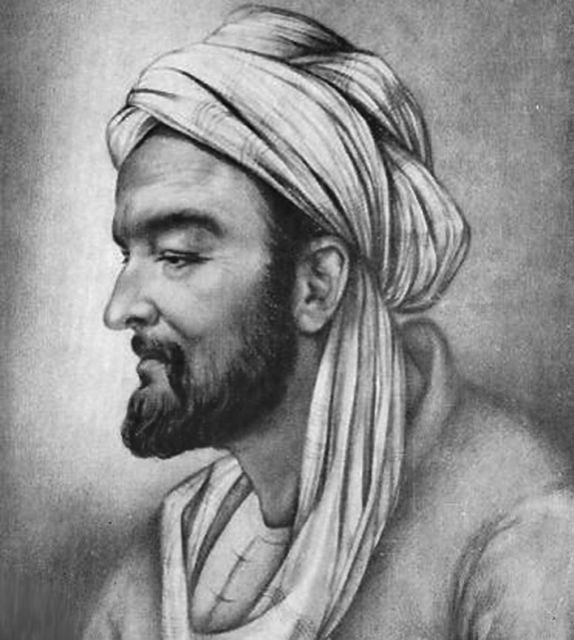
\includegraphics[width=5cm]{images/abu_ali.jpg}
  \caption*{«Коль смолоду избрал к заветной правде путь, \\
 С невеждами не спорь, советы их забудь». }
 \end{center}
\end{figure}


Каждый Мудрец может постигнуть Истину самостоятельно с вероятностью $1/9$ или же от соседа\footnote{Студенты постигают Истину примерно также!}. Независимо от способа постижения Истины, просветлённый Мудрец поделится Истиной с соседом слева с вероятностью $2/9$ и с соседом справа также с вероятностью $2/9$ (независимо от соседа слева).


\begin{enumerate}
\item Какова вероятность того, что Абу Али Хусейн ибн Абдуллах ибн аль-Хасан ибн Али ибн Сина постигнет Истину?
\item Как изменится ответ, если ряд Мудрецов бесконечен в обе стороны?
\end{enumerate}

\end{enumerate}

\subsection{Кр 1 ИП, 27.10.2016, решения}

\begin{enumerate}
\item
\begin{enumerate}
\item Для удобства занумеруем макаронины и выделим у каждой левый и правый конец. Взяли правый конец первой макаронины и подвязали случайной. Взяли свободный конец только что подвязанной макаронины и подвязали случайно. И так далее.
\[
\frac{2n-2}{2n-1}\cdot \frac{2n-4}{2n-3}\cdot \ldots \cdot \frac{2}{3} \cdot 1
\]
\item Допустим, что при $n$ макаронинах в среднем образуется $e_n$ колец. После первого соединения задача сводится к меньшему числу макаронин, важно только учесть, образовалось ли кольцо при первом соединении:
\[
e_n = e_{n-1} + 1/(2n-1) \cdot 1
\]
\item Количество коротких колец можно разбить в сумму, $X=Z_1 + \ldots + Z_n$. Вероятность завязывания конкретной макаронины в кольцо равна $1/(2n-1)$: «левый конец» надо привазять именно к «правому». Значит, $\E(X)=n/(2n-1)$.
\end{enumerate}

\item
\begin{enumerate}
\item Рассмотрим обратную ситуацию: на планете есть точка, из которой связаться хотя бы с одним пепелацем нельзя. Такое возможно, если все, кроме одного, сели в одну полуокружность.
\[
\P(\text{есть точка без связи}) = n \cdot \left(\frac{1}{2}\right)^{n-1} \Rightarrow \P(\text{из любой точки есть связь}) = 1 - n \cdot \left(\frac{1}{2}\right)^{n-1}
\]
\item Зафиксируем координату посадки первого пепелаца и возьмём её за точку отсчёта. Изобразим на плоскости возможные значения центральных углов между первым пепелацем и оставшимися и закрасим нужные участки. Получим 3/8.
\item Зафиксируем координату посадки первого пепелаца. Обозначим центральный угол между первым и вторым пепелацами $\alpha$. Функция плотности имеет вид: $p(\alpha) = \frac{\sin(\alpha)}{2}$

Итог: $\int_0^{\pi/2} p(\alpha) \frac{\alpha + \pi}{2\pi} d \alpha + \int_{\pi/2}^{\pi}  p(\alpha) \frac{\pi - \alpha}{2\pi} d \alpha = \frac{\pi + 2}{4\pi}$
\end{enumerate}

\item Вспомним для начала, что площадь круга равна $\pi r^2$, а площадь сферы равна $4\pi r^2$. Составим из маленьких треугольничков многогранник очень похожий на сферу с единичным радиусом. Площадь этого многогранника будет примерно равна $4\pi$. Проекция многогранника представляет собой примерно круг единичного радиуса. Проекция имеет два слоя. С учётом обоих слоёв площадь проекции равна $2\pi$. Значит отношение площади проекции к площади многогранника равно $1/2$.

От взаимного расположения треугольничков в пространстве ожидаемая площадь проекции не зависит в силу аддитивности математического ожидания.

Ответ: 21 см$^2$.

\item
\begin{enumerate}
\item Мысленно отметим на окружности три точки: места ударов Брюса Ли и точку, где схватился Чак Норрис. Можно считать, что эти три точки равномерно и независимо распределены по окружности. Следовательно, среднее расстояние между соседними точками равно $1/3$. Чак Норрис берёт два кусочка, слева и справа от своей точки. Значит ему в среднем достаётся $2/3$ окружности.
\item Объявим точку, где схватился Чак Норрис нулём. Координаты двух ударов изобразим на плоскости. Закрашиваем подходящий участок. Вероятность того, что кусок Брюса Ли длиннее, равна $1/4$.
\end{enumerate}

\item  Рассмотрим совершенно конкурентный невольничий рынок начинающих певиц. Певицы в хорошем настроении продаются по $V_1$, в депрессии — по $V_2$. Получаем систему уравнений:
\[
\begin{cases}
  V_1 = 0.75 + (0.5 V_1 + 0.5 V_2) \\
  V_2 = \max_x \sqrt{x}V_1 + (1 - \sqrt{x})V_2 - x
\end{cases}
\]
Оптимизируем и получаем, $x^* = (V_1 - V_2)^2/4$. Из первого уравнения находим $(V_1 - V_2)/2=0.75$.

\item Да. Например, такая. До общения с Джульеттой подкидывать монетку до выпадения первого орла и запомнить число потребовавшихся подбрасываний. Пусть это будет число $X$. Открыть равновероятно левую или правую руку Джульетты. Если открытое число больше $X$, то сказать, что оно большее, иначе сказать, что меньшее.
\item Если $\gamma$ — вероятность самостоятельного познания Истины, а $\alpha$ — передачи Истины отдельно в каждую из сторон, то
\[
p = \gamma + (1-\gamma) p \alpha.
\]

То есть $p=\gamma/(1-\alpha(1-\gamma))$.

Для решения второго пункта наложим на Абу Али Хусейн ибн Абдуллах ибн аль-Хасан ибн Али ибн Сина обет молчания. Это не повлияет на вероятность постижения им Истины, однако превратит задачу в две уже решённых :) Получаем
\[
q = \gamma + (1-\gamma)(2p\alpha - p^2\alpha^2)
\]
\end{enumerate}


\subsection{Кр 2 базовый поток, 09-12-2016}


\textbf{Неравенства Берри–Эссеена:} Для любых $n \in \mathbb{N}$ и всех $x \in \mathbb{R}$ имеет место оценка:
\[
    \bigl|F_{S_n^{*}}(x) - \Phi(x)\bigr| \leq 0.48 \cdot \frac{\E(|\xi_i - \E\xi_i|^3)}{\Var^{3/2}(\xi_i)\cdot\sqrt{n}} \text{,}
\]
где $\Phi(x) = \int_{-\infty}^{x}\frac{1}{\sqrt{2\pi}}e^{-\frac{t^2}{2}}\,dt$, \; $S_n^* = \frac{S_n - \E(S_n)}{\sqrt{\Var(S_n)}}$, \; $S_n = \xi_1 + \ldots + \xi_n$

\textbf{Распределение Пуассона:} Случайная величина $\xi$ имеет распределение Пуассона с параметром $\lambda > 0$,  если она принимает целые неотрицательные значения с вероятностями $\P(\{\xi = k\}) = \frac{\lambda^k}{k!}e^{-\lambda}$. Приличным студентам должно быть известно, что в этом случае $\E(\xi) = \Var(\xi) = \lambda$.

\begin{enumerate}
\item Пусть $\E(\xi) = 1$, $\E(\eta) = -2$, $\Var(\xi) = 1$, $\E(\eta^2) = 8$, $\E(\xi \eta) = -1$. Найдите
\begin{enumerate}
\item $\E(2\xi-\eta+1)$, $\Cov(\xi, \,\eta)$, $\Corr(\xi, \,\eta)$,  $\Var(2\xi-\eta+1)$;
\item $\Cov(\xi+\eta, \,\xi+1)$, $\Corr(\xi+\eta, \,\xi+1)$, $\Corr(\xi+\eta-24, \,365 - \xi - \eta)$, $\Cov(2016\cdot\xi, \, 2017)$.
\end{enumerate}

\item
Совместное распределение доходностей акций двух компаний задано с помощью таблицы:

\begin{center}
\begin{tabular}{c|cc}
\toprule
         & $\eta=-1$ & $\eta=1$ \\
\midrule
$\xi=-1$  & $0.1$       & $0.2$   \\
$\xi=0$   & $0.2$       & $0.2$   \\
$\xi=2$   & $0.2$       & $0.1$   \\
\bottomrule
\end{tabular}
\end{center}

\begin{enumerate}
  \item Найдите частные распределения случайных величин $\xi$ и $\eta$.
  \item Найдите $\Cov(\xi,\,\eta)$.
  \item Сформулируйте определение независимости дискретных случайных величин.
  \item Являются ли случайные величины $\xi$ и $\eta$ независимыми?
  \item Найдите условное распределение случайной величины $\xi$, если $\eta = 1$.
  \item Найдите условное математическое ожидание случайной величины $\xi$, если $\eta = 1$.
  \item Найдите математическое ожидание и дисперсию величины $\pi = 0.5\, \xi + 0.5\, \eta$.
  \item Рассмотрим портфель, в котором $\alpha$ — доля акций с доходностью $\xi$ и $(1 - \alpha)$ — доля акций с доходностью $\eta$. Доходность этого портфеля есть случайная величина
  \[\pi(\alpha) = \alpha \xi + (1-\alpha)\eta.\]
  Найдите такую долю $\alpha \in [0;\,1]$, при которой доходность портфеля $\pi(\alpha)$ имеет наименьшую дисперсию.
\end{enumerate}

\item Число посетителей сайта \url{pokrovka11.wordpress.com} за один день имеет распределение Пуассона с математическим ожиданием 250.
\begin{enumerate}
  \item Сформулируйте неравенство Маркова. При помощи данного неравенства оцените вероятность того, что за один день сайт посетят более 500 человек.
  \item Сформулируйте неравенство Чебышева. Используя данное неравенство, определите наименьшее число дней, при котором с вероятностью не менее 99\% среднее за день число посетителей будет отличаться от 250 не~более чем на 10.
  \item Решите предыдущий пункт с помощью центральной предельной теоремы.
  \item Сформулируйте закон больших чисел. Обозначим через $\xi_i$ число посетителей сайта за $i$-ый день. Найдите предел по вероятности последовательности $\frac{\xi_1^2 + \ldots + \xi_n^2}{n}$ при $n \rightarrow \infty$.
\end{enumerate}

\item Отведав медовухи, Винни–Пух совершает случайное блуждание на прямой. Он стартует из начала координат и в каждую следующую минуту равновероятно совершает шаг единичной длины налево или направо. Передвижения Винни-Пуха схематично изображены на следующем рисунке.
\begin{figure}[h]
    \noindent\centering{
    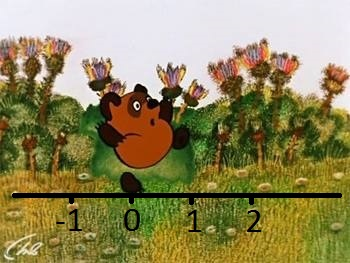
\includegraphics[width=80mm]{images/Winnie_the_Pooh_and_Medovuh.jpg}
    }
    \caption{Случайные бродилки.}
    \label{wun762hkej}
\end{figure}
\begin{enumerate}
  \item Сформулируйте центральную предельную теорему.
  \item При помощи центральной предельной теоремы оцените вероятность того, что ровно через час блужданий Винни-Пух окажется в области $(-\infty; \, -5]$.
  \item Используя неравенство Берри–Эссеена оцените погрешность вычислений предыдущего пункта.
\end{enumerate}


\item
Cлучайные величины $\xi$ и $\eta$ означают время безотказной работы рулевого управления и двигателя автомобиля соответственно. Время измеряется в годах. Совместная плотность имеет вид:
\[
f_{\xi, \,\eta}(x,\,y) =
\begin{cases}
0.005\,e^{-0.05\,x-0.1\,y} & \text{ при } x > 0, y > 0, \\
0                    & \text{ иначе.}
\end{cases}
\]

\begin{enumerate}
  \item Найдите частные плотности распределения случайных величин $\xi$ и $\eta$.
  \item Являются ли случайные величины $\xi$ и $\eta$ независимыми?
  \item Найдите вероятность того, что двигатель прослужит без сбоев более пяти лет.
  \item Найдите вероятность того, что двигатель прослужит без сбоев более восьми лет, если он уже проработал без сбоев три года.
  \item Найдите условное математическое ожидание безотказной работы рулевого управления, если двигатель проработал без сбоев пять лет,  $\E(\xi | \eta = 5)$.
  \item Найдите вероятность того, что рулевое управление проработает без сбоев на два года больше двигателя,  $\P(\{\xi - \eta > 2\})$.
\end{enumerate}

\item Бонусная задача

Случайная величина $\xi$ имеет плотность распределения
\[
    f_{\xi}(x) = \frac{1}{2} \cdot \frac{1}{\sqrt{2\pi}}e^{-\frac{(x-1)^2}{2}} + \frac{1}{2} \cdot \frac{1}{\sqrt{2\pi}}e^{-\frac{(x+1)^2}{2}} \text{.}
\]

\begin{enumerate}
\item Найдите $\E(\xi)$, $\E(\xi^2)$, $\Var(\xi)$.
\item Покажите, что функция $f_{\xi}(x)$, действительно, является плотностью распределения.
\end{enumerate}


\end{enumerate}



\subsection{Кр 2 базовый поток, 09-12-2016, решения}

\begin{enumerate}
\item \begin{enumerate}
\item $\E (2\xi - \eta +1) = 2 \E (\xi) - \E (\eta) + 1 = 2\cdot 1 - (-2) + 1 = 5 $

$\Cov (\xi, \eta) = \E (\xi \eta) - \E(\xi) \E(\eta) = -1 - \cdot 1 \cdot (-2) = 1$

$\Corr (\xi, \eta) = \frac{\Cov(\xi, \eta)}{\sqrt[]{\Var(X) \cdot \Var(Y)}} = \frac{1}{\sqrt{1 \cdot (8-(-2)^2)}} = \frac{1}{2}$

$\Var (2\xi - \eta + 1) = 4\Var(\xi) + \Var(\eta) - 2 \Cov (2\xi, \eta) = 4 \cdot 1 + 4 - 4 \cdot 1 = 4$

\item $\Cov(\xi + \eta, \xi + 1) = \Cov(\xi) + \Cov(\xi, 1) + \Cov(\eta, \xi) + \Cov(\eta, 1) = 1 +1 = 2$

$\Corr(\xi + \eta , \xi + 1) = \frac{\Cov(\xi + \eta , \xi + 1)}{\sqrt{\Var(\xi + \eta)\cdot \Var (\xi + 1)}} = \frac{2}{\sqrt{(1+4+2\cdot 1) \cdot 1}} = \frac{2}{\sqrt{7}}$

$\Corr(\xi + \eta - 24, 365 - \xi - \eta) = -1$

$\Cov(2016\cdot \xi, 2017) = 0$

\end{enumerate}
\item \begin{enumerate}
\item \begin{tabular}{cccc}
\toprule
$\xi$ & $-1$ & $0$ & $2$ \\ \midrule
$\P(\cdot)$ & $0.3$ & $0.4$ & $0.3$ \\ \bottomrule
\end{tabular}
\hspace{1cm}
\begin{tabular}{ccc}
\toprule
$\eta$ & $-1$ & $1$ \\ \midrule
$\P(\cdot)$ & $0.5$ & $0.5$ \\ \bottomrule
\end{tabular}

$\E(\xi) = -1 \cdot 0.3 + 0 \cdot 0.4 + 2 \cdot 0.3 = 0.3$

$\E (\xi^2) = (-1)^2 \cdot 0.3 + 0^2 \cdot 0.4 + 2^2 \cdot 0.3 = 1.5$

$\Var(\xi) = \E(\xi^2) - (\E(\xi))^2 = 1.5 - 0.3^2 = 1.41$

$\E(\eta) = -1 \cdot 0.5 + 1 \cdot 0.5 = 0$

$\E(\eta^2) = (-1)^2 \cdot 0.5 + 1^2 \cdot 0.5 = 1$

$\Var(\eta) = \E(\eta^2)-(\E(\eta))^2 = 1 - 0^2 = 1$

\item \begin{tabular}{cccccc}
\toprule
$\xi \cdot \eta$ & $-2$ & $-1$ & $0$ & $1$ & $2$ \\ \midrule
$\P(\cdot)$ & $0.2$ & $0.2$ & $0.4$ & $0.1$ & $0.1$ \\ \bottomrule
\end{tabular}

$\E(\xi\cdot\eta) = (-2) \cdot 0.2 + (-1) \cdot 0.2 + 0 \cdot 0.4 + 1\cdot 0.1 + 2 \cdot 0.1 = -0.3$

$\Cov(\xi, \eta) = \E(\xi\cdot\eta) - \E(\xi)\cdot\E(\eta) = -0.3 - 0.3 \cdot 0 = -0.3$
\item Пусть случайная величина $X$ принимает значения $a_1, \ldots, a_m$, случайная веилчина $Y$ принимает значения $b_1, \ldots, b_n$. Тогда случйаня величина $X$ и $Y$ называются независимыми, если $\forall i=1, \ldots, m \quad \forall j=1, \ldots, n: \P(X = a_i \cap Y = b_j) = P(X = a_i) \cdot P(Y = b_j)$
\item Заметим, что $\P (\xi = -1 \cap \eta=-1)=0.1$, $\P(\xi=-1)=0.3$ и $\P(\eta=-1)=0.5$.

Тогда поскольку $\P (\xi = -1 \cap \eta=-1) \neq \P(\xi=-1) \cdot \P(\eta=-1)$, случайные величины $\xi$ и $\eta$ не являются независимыми.
\item $\P (\xi = -1 \cap \eta=1) = \frac{\P (\xi = -1 \cap \eta=1)}{\P(\eta=1)} = \frac{0.2}{0.5} = \frac{2}{5}$

$\P (\xi = 0 \cap \eta=1) = \frac{\P (\xi = 0 \cap \eta=1)}{\P(\eta=1)} = \frac{0.2}{0.5} = \frac{2}{5}$

$\P (\xi = 2 \cap \eta=1) = \frac{\P (\xi = 2 \cap \eta=1)}{\P(\eta=1)} = \frac{0.1}{0.5} = \frac{1}{5}$

Следовательно, условное распределение случайной величины $\xi$ при условии $\{\eta=1\}$ может быть описано следующей таблицей:

\begin{tabular}{cccc}
\toprule
$\xi$ & $-1$ & $0$ & $2$ \\ \midrule
$\P(\cdot)$ & $2/5$ & $2/5$ & $1/5$ \\ \bottomrule
\end{tabular}
\item $\E(\xi \mid \eta = 1) = -1 \cdot \frac{2}{5} + 0 \cdot \frac{2}{5} + 2 \cdot \frac{1}{5} = 0$
\item $\E(\pi) = \E(0.5 \xi + 0.5 \eta) = 0.5 \E(\xi) + 0.5 \E(\eta) = 0.15$

\begin{multline*}
\Var(\pi) = \Var(0.5 \xi + 0.5 \eta) = \Var(0.5 \xi) + \Var(0.5\eta) + 2 \Cov (0.5\xi, 0.5\eta) = \\
= 0.25\Var(\xi) + 0.25\Var(\eta) + 2 \cdot 0.5 \cdot 0.5 \Cov(\xi, \eta) = \\
= 0.25 \cdot 1.41 + 0.25 \cdot 1 + 2 \cdot 0.5 \cdot 0.5 \cdot (-0.3) = 0.4525
\end{multline*}
\item
\begin{multline*}
\Var(\pi(\alpha)) = \Var(\alpha \xi + (1-\alpha)\eta) = \alpha^2\Var(\xi) + (1-\alpha)^2 \Var(\eta) + \\
+ 2\alpha(1-\alpha) \Cov(\xi, \eta) = 1.41 \cdot \alpha^2 + 1\cdot (1-\alpha)^2 + 2\alpha(1-\alpha) \cdot (-0.3) = \\
= 1.41 \cdot \alpha^2 + (1-\alpha)^2 - 0.6 \cdot (\alpha - \alpha^2) \to \min_\alpha
\end{multline*}
\begin{multline*}
\frac{\partial}{\partial \alpha} \Var(\pi(\alpha)) = 2 \cdot 1.41 \cdot \alpha -2(1-\alpha) -0.6\cdot(1-2\alpha) = \\
= 2.82 \cdot \alpha - 2 + 2\alpha - 0.6 + 1.2 \cdot \alpha = 6.02 \cdot \alpha - 2.6 = 0
\end{multline*}
\[
\alpha = \frac{2.6}{6.02} = 0.4319
\]
\end{enumerate}
\item \begin{enumerate}
\item Для любой неотрицательной случайной величины $X$ и любого числа $\lambda > 0$ справедлива оценка: $\P(X>\lambda) \leq \frac{\E(X)}{\lambda}$

Пусть случайная величина $\xi_i$ означает число посетителей сайта за $i$-ый день. По условию, $\xi_i \sim Pois(\lambda=250)$. Известно, что если $\xi \sim Pois(\lambda)$, то $\E(\xi) = \Var(\xi) = \lambda$.

Имеем:
\[
\P(\xi_i >500) \leq \P(\xi_i \geq 500) \leq \frac{\E(\xi_i)}{500} = \frac{250}{500} = \frac{1}{2}
\]
\item Для любой случайной величины $X$ с конечным $\E(X)$ и любого положительного числа $\epsilon > 0$ имеет место неравенство: $\P(X-\E(X)\geq\epsilon)\leq\frac{\Var(X)}{\epsilon^2}$

Обозначим $\bar{\xi}_n := \frac{1}{n} \left(\xi_1 + \ldots + \xi_n\right)$ – среднее число посетителей сайта за $n$ дней. Тогда
\[
\E(\bar{\xi}_n) = \E\left(\frac{1}{n} \sum_{i=1}^{n} \xi_i\right) = \frac{1}{n} \sum_{i=1}^{n} \E(\xi_i) = \frac{1}{n} \cdot n \cdot \lambda = \lambda = 250
\]
\[
\Var(\bar{\xi}_n) = \Var\left(\frac{1}{n} \sum_{i=1}^{n} \xi_i\right) = \frac{1}{n^2} \sum_{i=1}^{n} \Var (\xi_i) = \frac{n \cdot \lambda}{n^2} = \frac{\lambda}{n} = \frac{250}{n}
\]
Оценим вероятность
\[
\P(\vert\bar{\xi}_n-250\vert > 10) \leq \frac{\Var(\bar{\xi}_n)}{100} = \frac{250}{100\cdot n}
\]
Следовательно, $1 - \frac{250}{100\cdot n} \leq \P(\vert\bar{\xi}_n-250\vert > 10)$.

Найдём наименьшее целое $n$, при котором $0.99 \leq 1 - \frac{250}{100\cdot n}$.

Имеем:
\[
0.99 \leq 1 - \frac{250}{100\cdot n} \Leftrightarrow \frac{250}{100\cdot n} \Leftrightarrow n \geq \frac{250}{100 \cdot 0.01} \Leftrightarrow n  \geq 250
\]
Стало быть, $n=250$ – наименьшее число дней, при котором с вероятностью не менее $99\%$ среднее число поситителей будет отличаться от $250$ не более чем на $10$.
\item  Требуется найти наименьшее целое $n$, при котором $\P(\vert\bar{\xi}_n-250\vert \leq 10)=0.99$

Имеем:
\begin{multline*}
\P(\vert\bar{\xi}_n-250\vert \leq 10)=0.99 \Leftrightarrow \P(-10\leq \bar{\xi}_n -250 \leq 10) =0.99 \Leftrightarrow \\
\Leftrightarrow  \P(-10n \leq S_n-250 \leq 10n) =0.99
\end{multline*}
\[
\E(S_n) = \E(\xi_1 + \ldots + \xi_n) = \E(\xi_1) + \ldots + \E(\xi_n) = 250\cdot n
\]
\[
\Var(S_n) = \Var(\xi_1 + \ldots + \xi_n) = \Var(\xi_1) + \ldots + \Var(\xi_n) = 250 \cdot n
\]
\begin{multline*}
\P\left(\frac{-10n}{\sqrt{250n}} \leq \frac{S_n - \E (S_n)}{\sqrt{\Var(S_n)}} \leq \frac{10n}{\sqrt{250n}}\right) =0.99 \Leftrightarrow 2 \Phi \left(\frac{10n}{\sqrt{250n}}\right) -1 = 0.99 \\
\Phi \left(\frac{10n}{\sqrt{250n}}\right) = \frac{1 + 0.99}{2} \Leftrightarrow \frac{10n}{\sqrt{250n}} = 2.58 \Leftrightarrow \sqrt{n} = 2.58 \cdot \frac{\sqrt{250}}{10} \Leftrightarrow n = 16.641
\end{multline*}
Следовательно, наименьшее целое $n$, есть $n=17$.
\item Пусть $X_1, X_2, \ldots, X_n, \ldots$ – последовательность независимых случайных величин с одинаковыми конечными математическими ожиданимяи и фиксированными конечными дисперсиями. Тогда $\frac{X_1 + \ldots + X_n}{n} \stackrel{\P}{\to} \E(X_i)$ при $n \to \infty$.

В нашем случае случаные величины $\xi_1^2, \xi_2^2, \ldots, \xi_n^2, \ldots$ – независимы,

$\E(\xi_1^2) = \ldots = \E(\xi_n^2) = \ldots < + \infty$ и $\Var(\xi_1^2) = \ldots = \Var(\xi_n^2) = \ldots < + \infty$ . Поэтому в соответствии с ЗБЧ имеем:
\[
\frac{\xi_1^2 +\ldots+ \xi_n^2}{n} \stackrel{\P}{\to} \E(\xi_i^2) = \Var(\xi_i) +\E(\xi_i)^2 = \lambda + \lambda^2 = \lambda(\lambda+1) = 250\cdot251 = 62700
\]
\end{enumerate}

\item \begin{enumerate}
\item Пусть $X_1, X_2, \ldots, X_n, \ldots$ – последовательность независимых, одинаково распределённых случайных величин с $0<\Var(X_i)<\infty$, $i \in \mathbb{N}$.  Тогда для любого (борелевского) множества $B \subseteq R$ имеет место $\lim_{n \to \infty} \P\left(\frac{S_n - \E(S_n)}{\sqrt{\Var(S_n)}} \in B\right) = \int_B \frac{1}{\sqrt{2\pi}}e^{-t^2/2} dt$, где $S_n := X_1, \ldots, X_n$, $n \in \mathbb{N}$.
\item Введём случайную величину
\[
X_i = \begin{cases}
1, & \text{если на i-ом шаге Винни-Пух пошёл направо} \\
0, & \text{если пошёл налево}
\end{cases}
\quad i=1,\ldots, n;
\]
Тогда $S_n := X_1 +\ldots+X_n$ означает местоположение Винни-Пуха в $n$-ую минуту его блужданий по прямой.

$\E(X_i) = -1 \cdot 1/2 + 1 \cdot 1/2 = 0$,

$\E(X_i^2) = (-1)^2 \cdot 1/2 + (1)^2 \cdot 1/2 = 1$,

$\Var(X_i) = \E(X_i^2) - \E(X_i)^2 = 1$,

$\E(S_n) = \E(X_1 + \ldots + X_n ) = \E(X_1) + \ldots + \E(X_n) = 0$,

$\Var(S_n) = \Var(X_1 + \ldots + X_n ) = \Var(X_1) + \ldots + \Var(X_n) = n$

\begin{multline*}
\P(S_n \in (-\infty, -5]) = \P(S_n \leq -5) = \P\left( \frac{S_n-\E(S_n)}{\sqrt{\Var(S_n)}} \leq \frac{-5-0}{\sqrt{n}} \right) \stackrel{n=60}{=} \\
=\P\left( \frac{S_n-\E(S_n)}{\sqrt{\Var(S_n)}} \leq -0.6454\right) \approx \int_{-\infty}^{-0.6454} \frac{1}{\sqrt{2\pi}} e^{-t^2/2} dt = \\
= \Phi(-0.6454) = 1-\Phi(0.6454) \approx0.2593
\end{multline*}
\item Для любых $n \in \mathbb{N}$ и всех $x \in \mathbb{R}$ имеет место оценка:
\[
\bigl|F_{S_n^{*}}(x) - \Phi(x)\bigr| \leq 0.48 \cdot \frac{\E(|\xi_i - \E\xi_i|^3)}{\Var^{3/2}(\xi_i)\cdot\sqrt{n}} \text{,}
\]
где $\Phi(x) = \int_{-\infty}^{x}\frac{1}{\sqrt{2\pi}}e^{-\frac{t^2}{2}}\,dt$, \; $S_n^* = \frac{S_n - \E(S_n)}{\sqrt{\Var(S_n)}}$, \; $S_n = \xi_1 + \ldots + \xi_n$

В нашем случае:
\[
\P\left( \frac{S_{60} - \E(S_{60})}{\sqrt{\Var(S_{60})}} \leq -0.6454 \right) = \P(S^*_{60} \leq -0.6454) =
F_{S^*_{60}} (-0.6454)
\]
Согласно неравенству Берри-Эссеена, погрешность $\vert F_{S^*_{60}} (-0.6454) - \Phi(-0.6454) \vert$ оценивается сверху величиной
\[
0.48 \cdot \frac{\E(\vert X_i - \E(X_i) \vert^3 )}{\Var(X_i)^{3/2} \cdot \sqrt{n}} = 0.48 \cdot \frac{\E(\vert X_i \vert^3)}{1\cdot\sqrt{60}} = \frac{0.48}{\sqrt{60}} \approx0.062
\]
\end{enumerate}
\item \begin{enumerate}
\item Сначала найдём плотность распределения случайной величины $X$. Пусть $x \leq 0 $, тогда $f_X (X) = \int_{-\infty}^{+\infty} f_{X, Y} (x, y) dy  = 0$;

Пусть $x >0 $, тогда
\begin{multline*}
f_X (X) = \int_{-\infty}^{+\infty} f_{X, Y} (x, y) dy = \int_{0}^{+\infty} 0.005 e^{-0.05x-0.1y} dy = \\
= 0.005e^{-0.05x} \int_{0}^{+\infty} e^{-0.1y} dy = 0.005e^{-0.05x} \cdot \left(-10e^{-0.1y} \right) \bigg\vert_{y=0}^{y=+\infty} = 0.05 e^{-0.05x}
\end{multline*}
Таким образом, имеем:
\[
f_X (x) = \begin{cases}
0.05 e^{-0.05x} & \text{при } x>0 \\
0 & \text{при } x \leq 0
\end{cases}
\]
То есть $X \sim Exp(\lambda=0.05)$ – случайная величина $X$ имеет показательное распределение с параметром $\lambda = 0.05$.

Теперь найдём плотность распределения случайной величины $Y$.

Пусть $y \leq 0 $, тогда $f_Y (y) = \int_{-\infty}^{+\infty} f_{X, Y} (x, y) dx  = 0$.

Пусть $y > 0 $, тогда
\begin{multline*}
f_Y (y) = \int_{-\infty}^{+\infty} f_{X, Y} (x, y) dx  = \int_{0}^{+\infty} 0.005 e^{-0.05x-0.1y} dx = \\
= 0.005e^{-0.1y} \int_{0}^{+\infty} e^{-0.05x} dx = 0.005e^{-0.1y} \cdot \left(-20e^{-0.05x} \right) \bigg\vert_{x=0}^{x=+\infty} = 0.1 e^{-0.1y}
\end{multline*}
Таким образом, имеем:
\[
f_Y (y) = \begin{cases}
0.1 e^{-0.1y} & \text{при } y>0 \\
0 & \text{при } y \leq 0
\end{cases}
\]
То есть $Y \sim Exp(\lambda=0.1)$ – случайная величина $Y$ имеет показательное распределение с параметром $\lambda = 0.1$.
\item Поскольку для любых точек $x, y \in \mathbb{R}$ справедливо равенство $f_{X, Y} (x, y) = f_X (x) \cdot f_Y (y)$, случайные величины $X$ и $Y$ являются независимыми.
\item Найдём вероятность $\P(Y>5)$:
\[
\P(Y>5) = \int_{5}^{+\infty} f_Y (y) dy = \int_{5}^{+\infty}  0.1 e^{-0.1y} dy = 0.1 \cdot (-10 e^{-0.1x}) \bigg\vert_{y=5}^{y=+\infty} = e^{-0.5} \approx0.6065
\]
\item Требуется найти условную вероятность $\P(Y>8 \mid Y \geq 3)$. Для этого предварительно найдём вероятности $\P(Y>8)$ и $\P(y \geq 3)$:
\[
\P(Y>8) = \int_{8}^{+\infty} f_Y (y) dy  = \int_{8}^{+\infty}  0.1 e^{-0.1y} dy = 0.1 \cdot (-10 e^{-0.1x}) \bigg\vert_{y=8}^{y=+\infty} = e^{-0.8}
\]
\[
\P(Y \geq 3) =  \int_{3}^{+\infty} f_Y (y) dy   =  \int_{3}^{+\infty}  0.1 e^{-0.1y} dy = 0.1 \cdot (-10 e^{-0.1x}) \bigg\vert_{y=3}^{y=+\infty} = e^{-0.3}
\]
Теперь находим требуемую условную веростность:
\[
\P(Y>8 \mid Y \geq 3) = \frac{\P((Y > 8) \cap
(Y \geq 3))}{\P(Y \geq 3)} = \frac{\P(Y>8)}{\P(Y \geq 3) } = \frac{e^{-0.8}}{e^{-0.3}} = e^{-0.5} \approx0.6065
\]
\item Сначала найдём условную плотность распределения случайной величины $X$ при условии $Y=y$:
\begin{multline*}
f_{X \mid Y} (x \mid y) = \begin{cases}
\frac{f_{X \mid Y} (x, y)}{f_Y (y)} & \text{при } f_Y (y) 0 \\
0 & \text{иначе}
\end{cases} =
\begin{cases}
\frac{0.005e^{-0.05x-0.1y}}{0.1e^{-0.1y}} & \text{при } x>0, \quad y>0 \\
0 & \text{иначе}
\end{cases} = \\
= \begin{cases}
0.05 e^{-0.05x} & \text{при } x>0, \quad y>0 \\
0 & \text{иначе}
\end{cases} =
\begin{cases}
f_X (x) & \text{при } y > 0 \\
0 & \text{при } y \leq 0
\end{cases}
\end{multline*}
Теперь находим условное математическое ожидание
\[
\E(X \mid Y=5) = \int_{-\infty}^{+\infty} xf_{X\mid Y} (x \mid 5) dx =  \int_{-\infty}^{+\infty} xf_{X} (x) dx = \E(X) = \frac{1}{0.05} =20
\]
Здесь мы воспользовались известным фактом, что если $X\sim Exp(\lambda)$, то $\E(X) = \frac{1}{\lambda}$
\item Требуется найти вероятность $\P(X-Y > 2)$. Для этого введём множества

$B:=\{(x, y) \in \mathbb{R} : y < x-2 \}$ и $C := \{ (x,y) \in \mathbb{R} : y < x-2, x>0, y> 0  \}$.

Заметим, что искомая вероятность  $\P(X-Y > 2)$ может быть записана в виде
\[
\P(X-Y > 2) = \P((X, Y) \in B ) = \int \int_B f_{X, Y} (x, y) dx dy = \int \int_C f_{X, Y} (x, y) dx dy
\]
Стало быть, искомая вероятность
\begin{multline*}
\P(X-Y > 2) = \int \int_C f_{X, Y} (x, y) dx dy = \int_{2}^{+\infty} \left[ \int_{0}^{x-2} f_{X, Y} (x, y) dy \right] dx =\\
= \int_{2}^{+\infty} \left[ \int_{0}^{x-2} 0.005e^{-0.05x-0.1y}dy \right] dx
= \int_{2}^{+\infty} \left[ 0.005e^{-0.05x} \cdot (-10e^{-0.1y}) \bigg\vert_{y=0}^{y=x-2} \right] dx = \\
=  \int_{2}^{+\infty} \left[ 0.005e^{-0.05x} \cdot\left(1-e^{-0.1(x-2)}  \right) \right] dx  = \int_{2}^{+\infty} 0.005e^{-0.05x} dx - \\
- \int_{2}^{+\infty} 0.005e^{-0.05x-0.1x+0.2} dx
= 0.05 \cdot \left( -\frac{1}{0.05}e^{-0.05x}  \right) \bigg\vert_{x=2}^{x=+\infty} - \\
- e^{0.02} \cdot 0.05 \cdot \left( \frac{1}{0.15} e^{-0.15x} \right) \bigg\vert_{x=2}^{x=+\infty}
= e^{-0.1} -\frac{1}{3} e^{-0.1} = \frac{2}{3}e^{-0.1}  \approx 0.6032
\end{multline*}
\end{enumerate}
\item Для решения задачи воспользуемся хорошо известными соотношениями:
\[
\int_{-\infty}^{+\infty} \frac{1}{\sqrt{2\pi\sigma^2}} e^{-\frac{(x-\mu)^2}{2\sigma^2}} dx = 1
\]
\[
\int_{-\infty}^{+\infty} x\frac{1}{\sqrt{2\pi\sigma^2}} e^{-\frac{(x-\mu)^2}{2\sigma^2}} dx = \mu
\]
\[
\int_{-\infty}^{+\infty} x^2 \frac{1}{\sqrt{2\pi\sigma^2}} e^{-\frac{(x-\mu)^2}{2\sigma^2}} dx = \mu^2 + \sigma^2
\]
\begin{enumerate}
\item Указанная в задании функция $f_X$ является плотностью распределения, так как она удовлетворяет двум условиям:  $f_X$ является неотрицательной и интеграл от функции $f_X$ в пределах от  $-\infty$ до $+\infty$ равен единице:
\[
\int_{-\infty}^{+\infty} f_X (x) dx = \frac{1}{2} \cdot \int_{-\infty}^{+\infty}  \frac{1}{\sqrt{2\pi}} e^{-\frac{(x-1)^2}{2\sigma^2}} dx  + \frac{1}{2} \int_{-\infty}^{+\infty} \cdot \frac{1}{\sqrt{2\pi}} e^{-\frac{(x+1)^2}{2}} dx = 1
\]
\item $\E(X) =\int_{-\infty}^{+\infty} xf_X (x) dx =  \frac{1}{2} \cdot \int_{-\infty}^{+\infty} x \frac{1}{\sqrt{2\pi}} e^{-\frac{(x-1)^2}{2\sigma^2}} dx  + \frac{1}{2}\int_{-\infty}^{+\infty} \cdot x \frac{1}{\sqrt{2\pi}} e^{-\frac{(x+1)^2}{2}} dx = 1- 1=  0$
\item  \begin{multline*}
\E(X^2) = \int_{-\infty}^{+\infty} x^2 f_X (x) dx  =  \frac{1}{2} \cdot \int_{-\infty}^{+\infty} x^2 \frac{1}{\sqrt{2\pi}} e^{-\frac{(x-1)^2}{2\sigma^2}} dx  + \frac{1}{2} \int_{-\infty}^{+\infty}\cdot x^2 \frac{1}{\sqrt{2\pi}} e^{-\frac{(x+1)^2}{2}} dx = \\
= 1^2 + 1^2 + (-1)^2 + 1^2 =  2
\end{multline*}
\item $\Var(X) = \E(X^2) - (\E(X))^2 = 2 - 0^2 = 2$
\end{enumerate}
\end{enumerate}



\subsection{CosmoWar: blue part}

\begin{center}
ЭРА I
\end{center}

\begin{enumerate}
\item Исследуя образцы грунта планеты Броуни, межгалактическая экспедиция обнаружила в нем простейшую, но очень интересную одноклеточную форму жизни. От одной материнской клетки рождаются два потомка, причем сразу после рождения они начинают независимо двигаться вдоль одной и той же прямой и могут без проблем проходить друг через друга. Собрав статистику их передвижений, исследователи поняли, что $X_t$, положение клетки относительно места рождения в момент ее жизни $t$, распределено межгалактически нормально: $X_t\sim \mathcal{N}(0; t)$. Как далеко друг от друга в среднем оказываются потомки в момент $t$?


Подсказка: \textit{межгалактическое нормальное распределение совпадает с земным и имеет плотность}

$f_X(x) = \frac{1}{\sqrt{2\pi}\sigma}e^{-\frac{(x-\mu)^2}{2\sigma^2}}$.

\item В Солнечной системе есть по крайней мере $5$ карликовых планет: Плутон (до 2006 года считавшийся девятой планетой), Макемаке, Хаумеа, Эрида и Церера. Допустим, что Незнайка думает, что расстояние между Макемаке и Эридой равно $1$;  $X$~--- расстояние между Макемаке и Церерой~--- равномерно распределенная на отрезке от $0$ до $2$ случайная величина; $Y$~--- расстояние между Эридой и Церерой~--- экспоненциальная случайная величина с параметром $\lambda = 1$. Также Незнайка думает, что $X$ и $Y$ независимы. Найдите в представлении Незнайки вероятность того, что отрезки с длинами $X$, $Y$ и $1$ образуют треугольник.

\item  В системе Акаика-02 находится $p$ планет. Всю жизнь Пульпик путешествует с одной планеты на другую. При этом путь его лежит всегда через космическую станцию. Там он равновероятно выбирает новую планету, отправляется на её исследование и возвращается обратно. Пульпик начинает свою одиссею с космической станции. Пусть $A_0^{(n)}$ — это количество посещений космической станции через $n$ шагов, а $A_i^{(n)}$~--- количество посещений $i$-й планеты.

\begin{enumerate}
\item Найдите $\plim_{n \rightarrow \infty} \frac{A_0^{(n)}}{n}$
\item Найдите $\plim_{n \rightarrow \infty} \frac{A_i^{(n)}}{n}$
\end{enumerate}


\end{enumerate}



\begin{center}
ЭРА II
\end{center}

\begin{enumerate}
\item Пусть на Марсе живет $n$ семей, y каждой марсианской семьи есть некоторое количество марсианских детишек. $\xi_1, \ldots, \xi_n$~--- количество марсианских детишек в марсианских семьях~--- независимые одинаково распределенные случайные величины. Пусть $\vartheta_i = \dfrac{\xi_i}{\sum_{j = 1}^n \xi_j}$~--- уровень счастья $i$-й марсианской семьи. Найдите:

\begin{enumerate}
\item Математическое ожидание счастья $i$-й семьи.
\item Найдите $ \Corr (\vartheta_i, \vartheta_j)$
\end{enumerate}

\item Пусть на Марсе по-прежнему живет $n$ семей, у каждой марсианской семьи есть некоторое количество марсианских детишек. $Y_i$ — средний рост ребенка в $i$-ой марсианской семье -- независимые равномерно распределенные на отрезке $[0; 1]$ случайные величины. Марсианские ученые всерьез озаботились проблемой старения роста марсианского населения, но не знали, с чего начать свои исследования, поэтому сперва решили посчитать следующую величину:  $\varepsilon_n = \min \{Y_1, \ldots, Y_n\}$.

\begin{enumerate}
\item Найдите $\P (\varepsilon_n \leq x)$
\item Найдите $\lim_{n \rightarrow \infty} \P (n\varepsilon_n \leq x)$
\end{enumerate}

\item Астроном смотрит на случайно выбираемую звезду. Её яркость~--- случайная величина $\xi$. Число $A$~--- некоторая константа, выдуманная учеными для упрощения жизни, а именно для того, чтобы минимизировать выражение $\E(|\xi - A|)$. Найдите, чему равно $A$.
\end{enumerate}


\begin{center}
ЭРА III
\end{center}

\begin{enumerate}
\item Между планетами Кин и Дза существует небольшой торговый путь, по которому регулярно следуют грузовые шаттлы. Производство в секторе небольшое, так что больше одного грузового шаттла на пути не бывает. В неизвестный заранее момент пути торгового корабля в произвольном месте маршрута появляется пиратский звездолёт с излучателем, способным дистанционно и мгновенно похитить груз. Галактическая полиция на планете Кин тут же получает сигнал о присутствии пиратского корабля и может также мгновенно остановить ограбление, но только если расстояние от нее до звездолёта пиратов или шаттла торговцев меньше, чем между шаттлом торговцев и звездолётом пиратов. Что случается чаще~--- ограбления или спасения кораблей? Покажите формально.

\item Пусть имеется последовательность случайных величин $X_1, \ldots, X_n$, где $X_i$ равновероятно принимает значения $1, 2, \ldots, 100$. Пусть $A_0 = \varnothing$, тогда c вероятностью $1/3$: $A_n = A_{n-1} \backslash X_n$ и с вероятностью $2/3$: $A_n = A_{n-1} \cup X_n$.

\begin{enumerate}
\item Найдите математическое ожидание мощности множества $A_n$
\item Найдите $\lim_{n \rightarrow \infty} \E (|A_n|)$
\end{enumerate}

\item  Пульпик после долгих скитаний решил заняться наукой на планете Кондисиус. Однажды во время научных изысканий ему повстречались случайные матричные операторы. Но он никак не может посчитать, чему равно математическое ожидание длины отображенного вектора. ПОМОГИТЕ ПУЛЬПИКУ! Пусть $A_{s \times s}$ это случайная матрица, где каждый элемент имеет нормальное распределение с параметрами $0$ и $1/s$. Пусть имеется некоторый вектор $v_{s \times 1}$. Докажите, что $\E(||Av||^2) = ||v||^2$.
\end{enumerate}

\subsection{Kosmowar, blue part solutions, 24.12.2016}

\begin{enumerate}
\item Здесь могло быть ваше решение
\item По неравенству треугольника должны быть выполнены следующие условия
\begin{equation*}
\begin{cases}
X + Y > 1 \\
X + 1 > Y \\
Y  + 1 > X
\end{cases}
\end{equation*}
Получаем некоторую область на плоскости. Осталось посчитать вероятность оказаться там. Совместная функция плотности
\[
f(x, y) = \frac{e^{-y}}{2}
\]
Считаем интеграл
\[
\frac{1}{2}\left(  \int_{0}^1 \int_{1 - x}^{1 + x} e^{-y} dy dx  + \int_{1}^2 \int_{-1 + x}^{1 + x}  e^{-y} dy dx  \right)
\]
Первое слагаемое:
\begin{multline*}
 \int_{0}^1 \int_{1 - x}^{1 + x} e^{-y} dy dx = - \int_{0}^1 e^{-y} \bigg\vert_{1 - x}^{1 + x} dx = - \int_{0}^1 e^{-1 - x} - e^{- 1 + x} dx = \\
= \int_0^1 e^{-1} e^x dx - \int_{0}^1 e^{-1} e^{-x} dx = \left(1 -  \frac{1}{e}\right)^2
\end{multline*}
Второе слагаемое:
\begin{multline*}
\int_{1}^2 \int_{-1 + x}^{1 + x}  e^{-y} dy dx = - \int_{1}^2 e^{-y} \bigg\vert_{-1 + x}^{1 + x} dx = \int_1^2 e^{1 - x} - e^{- 1 - x} dx = \\
= e \int_1^2 e^{-x} dx - e^{-1} \int_1^2 e^{-x} dx = \left( e - \frac{1}{e}\right) \left( 1 - \frac{1}{e} \right) \frac{1}{e}  = \left( 1 + \frac{1}{e} \right) \left(1 -  \frac{1}{e}\right)^2
\end{multline*}
Итого:
\[
\frac{1}{2}\left(  \int_{0}^1 \int_{1 - x}^{1 + x} e^{-y} dy dx  + \int_{1}^2 \int_{-1 + x}^{1 + x}  e^{-y} dy dx  \right) = \frac{1}{2}  \left( 2 + \frac{1}{e} \right) \left(1 -  \frac{1}{e}\right)^2
\]
\item Всё просто. Мы посещаем центр после каждой планеты, последовательно посещений будет выглядеть так: $A_0, A_i, A_0, A_j, \ldots$, значит для центр это половина всех посещенных мест. Значит в первом пункте ответ $1/2$. Все остальные планеты  симметричны и посещения равномерно между ними распределяются, во втором пункте получаем $\frac{1}{2n}$.
\item Заметим, что $\sum_{i = 1}^n \vartheta_i = 1$. Взяв матожидание слева и справа получаем $\E \vartheta_i = \frac{1}{n}$. Корреляцию считаем также, заметим что
\[
\Corr (\sum_{i = 1}^n \vartheta_i, \vartheta_j) = 0
\]
\[
\sum_{i = 1}^n \Corr (\vartheta_i, \vartheta_j) = 0
\]
\[
\sum_{i \neq j}^n \Corr (\vartheta_i, \vartheta_j) = -1
\]
\[
(n-1)  \Corr (\vartheta_i, \vartheta_j) = -1
\]
\[
 \Corr (\vartheta_i, \vartheta_j) = \frac{-1}{n-1}
\]
\item \[
\P (\varepsilon_n \leq x) = 1 - \P (\varepsilon_n > x) = 1 - \prod_{i = 1}^n  \P (Y_i > x) = 1 - (1 - x)^n.
\]
Теперь второй пункт:
\begin{multline*}
\lim_{n \rightarrow \infty} \P (n\varepsilon_n \leq x) = \lim_{n \rightarrow \infty} \P (\varepsilon_n \leq x/n) =  \lim_{n \rightarrow \infty} 1 - \left(1 - \frac{x}{n}\right)^n = \\
= 1 - \lim_{n \rightarrow \infty} \left(1 - \frac{x}{n}\right)^n = 1 - e^{-x}
\end{multline*}
\item \[
\E |\xi - a| = \int_{-\infty}^a (a - x) dP(x) +  \int_{a}^{\infty} (x- a) dP(x)
\]
Воспользуемся формулой Ньютона — Лейбница и возьмём производную по $a$. Мы имеем право это сделать, так как интеграл сходится.
\[
\frac{\partial \E|\xi - a|}{\partial a} = \int_{-\infty}^a dP(x) - \int_{a}^{\infty} dP(x) = 0
\]
\[
\P(\xi \leq a) = \P(\xi > a)
\]
Следовательно $a$ это медиана.
\item Здесь могло быть ваше решение.

\item Рассмотрим поведение отдельного числа. С какой вероятностью оно будет присутствовать во множестве? С вероятностью $p_{n-1}$ оно уже было внутри, его уберут от туда с вероятностью $1/100 \cdot 1/3$, если его не было, то его добавят с вероятностью $1/100 \cdot 2/3$. Получаем
\[
p_n = \frac{299}{300}p_{n - 1} + \frac{2}{300}(1 - p_{n-1})
\]
\[
p_n = \frac{297}{300}p_{n - 1} +  \frac{2}{300}
\]
Получаем разностное уравнение, $\lambda = \frac{297}{300}$. Частное решение $C = \frac{2}{3}$. Начальное условие $p_0 = 0$.
\[
p_0 = A + \frac{2}{3} = 0
\]
\[
A = -\frac{2}{3}
\]
Решение:
\[
p_n = -\frac{2}{3} \cdot \left( \frac{297}{300} \right)^n + \frac{2}{3}
\]
Отлично, через индикаторы матожидание можно разложить на сумму вероятностей. Получаем:
\[
\E |A_n| = 100 p_n = -\frac{2 \cdot 100}{3} \cdot \left( \frac{297}{300} \right)^n + \frac{2 \cdot 100}{3}
\]
Берём предел и получаем
\[
\frac{2 \cdot 100}{3}
\]

\item \[
\E(||Av||^2) = \E \left(\sum_{i = 1}^s (Av)^2_{i} \right) = \sum_{i = 1}^s \E (Av)^2_{i}  = s \E (Av)^2_{i}
\]
\[
(Av)_i = \sum_{j= 1}^s \xi_{i, j} v_j
\]
Так как мы умножаем, то нормально распределенную случайную величину на константу, её дисперсия становится равной $\frac{v_j^2}{s}$. Сумма нормальных величин будет иметь дисперсию: $\frac{1}{s}\sum_{i = 1}^s v_i^2$. Тогда $\E (Av)^2_{i} = \frac{1}{s}\sum_{i = 1}^s v_i^2$. Умножаем на $s$ и получаем норму вектора $v$ в квадрате.


\end{enumerate}



\subsection{Экзамен за 1 семестр, 24.12.2016}

\element{midterm_2016}{ % в фигурных скобках название группы вопросов
 \AMCcompleteMulti
  \begin{questionmult}{1} % тип вопроса (questionmult — множественный выбор) и в фигурных — номер вопроса
  Граф Сен-Жермен извлекает карты в случайном порядке из стандартной колоды в 52 карты без возвращения. Рассмотрим три события: $A$ — «первая карта — тройка»; $B$ — «вторая карта — семёрка»; $C$ — «третья карта — дама пик».
 %\begin{multicols}{3} % располагаем ответы в 3 колонки
   \begin{choices} % опция [o] не рандомизирует порядок ответов
      \correctchoice{События $A$ и $B$ зависимы, события $B$ и $C$ зависимы.}
      \wrongchoice{События $A$ и $B$ независимы, события $B$ и $C$ независимы.}
      \wrongchoice{События $A$ и $B$ независимы, события $B$ и $C$ зависимы.}
      \wrongchoice{События $A$ и $B$ зависимы, события $B$ и $C$ независимы.}
      \wrongchoice{События $A$ и $С$ независимы, события $B$ и $C$ зависимы.}
      \end{choices}
  %\end{multicols}
  \end{questionmult}
}



\element{midterm_2016}{ % в фигурных скобках название группы вопросов
 \AMCcompleteMulti
  \begin{questionmult}{2} % тип вопроса (questionmult — множественный выбор) и в фигурных — номер вопроса
Монетку подбрасывают три раза. Рассмотрим три события: $A$ — «хотя бы один раз выпала решка»; $B$ — «хотя бы один раз выпал орёл»; $C$ — «все три раза выпал орёл».
 %\begin{multicols}{3} % располагаем ответы в 3 колонки
   \begin{choices} % опция [o] не рандомизирует порядок ответов
     \correctchoice{События $A$ и $B$ совместны, события $A$ и $C$ несовместны.}
     \wrongchoice{События $A$ и $B$ несовместны, события $B$ и $C$ совместны.}
     \wrongchoice{События $A$ и $B$ несовместны, события $B$ и $C$ несовместны.}
     \wrongchoice{События $A$ и $B$ совместны, события $A$ и $C$ совместны.}
     \wrongchoice{События $A$ и $B$ несовместны, события $A$ и $C$ совместны.}
      \end{choices}
  %\end{multicols}
  \end{questionmult}
}


\element{midterm_2016_rejected}{ % в фигурных скобках название группы вопросов
 \AMCcompleteMulti
  \begin{questionmult}{3} % тип вопроса (questionmult — множественный выбор) и в фигурных — номер вопроса
  На шахматной доске в клетке A1 стоит белая ладья. На одну из оставшихся клеток случайным образом выставляется чёрная ладья. Вероятность того, что ладьи «бьют» друг друга равна
 \begin{multicols}{3} % располагаем ответы в 3 колонки
   \begin{choices} % опция [o] не рандомизирует порядок ответов
      \correctchoice{$14/63$}
      \wrongchoice{$1/2$}
      \wrongchoice{$16/64$}
      \wrongchoice{$14/64$}
      \wrongchoice{$16/63$}
      \wrongchoice{$15/64$}
      \end{choices}
  \end{multicols}
  \end{questionmult}
}


\element{midterm_2016}{ % в фигурных скобках название группы вопросов
 \AMCcompleteMulti
  \begin{questionmult}{3} % тип вопроса (questionmult — множественный выбор) и в фигурных — номер вопроса
  В школе три девятых класса: 9А, 9Б и 9В. В 9А классе — 50\% отличники, в 9Б — 30\%, в 9В — 40\%. Если сначала равновероятно выбрать один из трёх классов, а затем внутри класса равновероятно выбрать школьника, то вероятность выбрать отличника равна
 \begin{multicols}{3} % располагаем ответы в 3 колонки
   \begin{choices} % опция [o] не рандомизирует порядок ответов
      \correctchoice{$0.4$}
      \wrongchoice{$0.3$}
      \wrongchoice{$0.5$}
      \wrongchoice{$0.27$}
      \wrongchoice{$3/(3+4+5)$}
      \wrongchoice{$(3+4+5)/3$}
      \end{choices}
  \end{multicols}
  \end{questionmult}
}



\element{midterm_2016}{ % в фигурных скобках название группы вопросов
 \AMCcompleteMulti
  \begin{questionmult}{4} % тип вопроса (questionmult — множественный выбор) и в фигурных — номер вопроса
  Если $\P(A)=0.2$, $\P(B)=0.5$, $\P(A | B) = 0.3$, то
 \begin{multicols}{3} % располагаем ответы в 3 колонки
   \begin{choices} % опция [o] не рандомизирует порядок ответов
      \correctchoice{$\P(A \cap B) = 0.15$}
      \wrongchoice{$\P(A \cup B) = 0.8$}
      \wrongchoice{$\P(A \cap B) = 0.05$}
      \wrongchoice{$\P(A \cup B) = 0.7$}
      \wrongchoice{$\P(B \cup A) = 0.3$}
      \end{choices}
  \end{multicols}
  \end{questionmult}
}


\element{midterm_2016_rejected}{ % в фигурных скобках название группы вопросов
 \AMCcompleteMulti
  \begin{questionmult}{5} % тип вопроса (questionmult --- множественный выбор) и в фигурных — номер вопроса
  Традиционно себя называют Стрельцами люди, родившиеся с 22 ноября по 21 декабря. Из-за прецессии земной оси линия Солнце–Земля указывает в созведие Стрельца в наше время с 17 декабря по 20 января. Предположим, что все даты рождения равновероятны. Вероятность того, что человек, называющий себя Стрельцом, родился в день, когда линия Солнце–Земля указывала в созвездие Стрельца, равна
 \begin{multicols}{3} % располагаем ответы в 3 колонки
   \begin{choices} % опция [o] не рандомизирует порядок ответов
      \correctchoice{$5/30$}
      \wrongchoice{$4/30$}
      \wrongchoice{$4/31$}
      \wrongchoice{$1/2$}
      \wrongchoice{$4/35$}
      \end{choices}
  \end{multicols}
  \end{questionmult}
}


\element{midterm_2016}{ % в фигурных скобках название группы вопросов
 \AMCcompleteMulti
  \begin{questionmult}{5} % тип вопроса (questionmult --- множественный выбор) и в фигурных — номер вопроса
  Монетка выпадает орлом с вероятностью $0.2$. Вероятность того, что при 10 подбрасываниях монетка выпадет орлом хотя бы один раз, равна
 \begin{multicols}{3} % располагаем ответы в 3 колонки
   \begin{choices} % опция [o] не рандомизирует порядок ответов
      \correctchoice{$1 - 0.8^{10}$}
      \wrongchoice{$2/10$}
      \wrongchoice{$0.2^{10}$}
      \wrongchoice{$1/2$}
      \wrongchoice{$C_{10}^1 0.2^{1}0.8^9$}
      \wrongchoice{$C_{10}^1 0.8^{1}0.2^9$}
      \end{choices}
  \end{multicols}
  \end{questionmult}
}


\element{midterm_2016}{ % в фигурных скобках название группы вопросов
 \AMCcompleteMulti
  \begin{questionmult}{6} % тип вопроса (questionmult — множественный выбор) и в фигурных — номер вопроса
  Среди покупателей магазина мужчин и женщин поровну. Женщины тратят больше 1000 рублей с вероятностью 60\%, а мужчины — с вероятностью 30\%. Только что был пробит чек на сумму 1234 рубля. Вероятность того, что покупателем была женщина равна
 \begin{multicols}{3} % располагаем ответы в 3 колонки
   \begin{choices} % опция [o] не рандомизирует порядок ответов
      \correctchoice{$2/3$}
      \wrongchoice{$0.5$}
      \wrongchoice{$0.3$}
      \wrongchoice{$0.18$}
      \wrongchoice{$1/3$}
      \end{choices}
  \end{multicols}
  \end{questionmult}
}







\element{midterm_2016}{ % в фигурных скобках название группы вопросов
 \AMCcompleteMulti
  \begin{questionmult}{11} % тип вопроса (questionmult — множественный выбор) и в фигурных — номер вопроса
  Если $F_X(x)$ — функция распределения случайной величины, то
 \begin{multicols}{2} % располагаем ответы в 3 колонки
   \begin{choices} % опция [o] не рандомизирует порядок ответов
      \correctchoice{ $\P(X \in (a;b] = F_X(b) - F_X(a)$}
      \wrongchoice{$F_X(x)$ может принимать отрицательные значения}
      \wrongchoice{величина $X$ дискретна}
      \wrongchoice{величина $X$ непрерывна}
      \wrongchoice{$\lim\limits_{x \rightarrow -\infty} F_X(x) = 1 $}
      \wrongchoice{$F_X(x)$ может принимать значение 2016}
      \end{choices}
  \end{multicols}
  \end{questionmult}
}



\element{midterm_2016}{ % в фигурных скобках название группы вопросов
 \AMCcompleteMulti
  \begin{questionmult}{12} % тип вопроса (questionmult — множественный выбор) и в фигурных — номер вопроса
Функцией плотности случайной величины может являться функция
 \begin{multicols}{2} % располагаем ответы в 3 колонки
   \begin{choices} % опция [o] не рандомизирует порядок ответов
     \correctchoice{$ f(x) = \begin{cases}
            \frac{1}{x^2}, x \in [1,+ \infty) \\
            0,\text{ иначе}
        \end{cases}  $}

     \wrongchoice{$ f(x) = \begin{cases}
     				x - 1, x \in [0,1+\sqrt{3}] \\
     				0,\text{ иначе}
 				\end{cases}  $}

     \wrongchoice{$ f(x) = \begin{cases}
     			  x^2, x \in [0,2] \\
     				0,\text{ иначе}
 				\end{cases}  $}



     \wrongchoice{$ f(x) = \begin{cases}
     				-1, x \in [-1, 0] \\
     				0,\text{ иначе}
 				\end{cases}  $}

     \wrongchoice{$ f(x) = \frac{1}{\sqrt{2\pi}} e^{-x^2}  $}

      \end{choices}
  \end{multicols}
  \end{questionmult}
}




\element{midterm_2016}{ % в фигурных скобках название группы вопросов
 \AMCcompleteMulti
  \begin{questionmult}{13} % тип вопроса (questionmult — множественный выбор) и в фигурных — номер вопроса
  Известно, что $\E(X)=3$, $\E(Y)=2$, $\Var(X)=12$, $\Var(Y)=1$, $\Cov(X,Y)=2$. Ожидание $\E(XY)$ равно
 \begin{multicols}{3} % располагаем ответы в 3 колонки
   \begin{choices} % опция [o] не рандомизирует порядок ответов
      \correctchoice{8}
      \wrongchoice{6}
      \wrongchoice{0}
      \wrongchoice{2}
      \wrongchoice{5}
      \end{choices}
  \end{multicols}
  \end{questionmult}
}




\element{midterm_2016}{ % в фигурных скобках название группы вопросов
 \AMCcompleteMulti
  \begin{questionmult}{14} % тип вопроса (questionmult — множественный выбор) и в фигурных — номер вопроса
  Известно, что $\E(X)=3$, $\E(Y)=2$, $\Var(X)=12$, $\Var(Y)=1$, $\Cov(X,Y)=2$. Корреляция $\Corr(X,Y)$ равна
 \begin{multicols}{3} % располагаем ответы в 3 колонки
   \begin{choices} % опция [o] не рандомизирует порядок ответов
      \correctchoice{$\frac{1}{\sqrt{3}}$}
      \wrongchoice{$\frac{2}{\sqrt{13}}$}
      \wrongchoice{$\frac{1}{12}$}
      \wrongchoice{$\frac{1}{\sqrt{12}}$}
      \wrongchoice{$\frac{2}{12}$}
      \end{choices}
  \end{multicols}
  \end{questionmult}
}



\element{midterm_2016}{ % в фигурных скобках название группы вопросов
 \AMCcompleteMulti
  \begin{questionmult}{15} % тип вопроса (questionmult — множественный выбор) и в фигурных — номер вопроса
  Известно, что $\E(X)=3$, $\E(Y)=2$, $\Var(X)=12$, $\Var(Y)=1$, $\Cov(X,Y)=2$. Дисперсия $\Var(2X-Y+4)$ равна
 \begin{multicols}{3} % располагаем ответы в 3 колонки
   \begin{choices} % опция [o] не рандомизирует порядок ответов
      \correctchoice{41}
      \wrongchoice{49}
      \wrongchoice{53}
      \wrongchoice{57}
      \wrongchoice{45}
      \end{choices}
  \end{multicols}
  \end{questionmult}
}



\element{midterm_2016}{ % в фигурных скобках название группы вопросов
 \AMCcompleteMulti
  \begin{questionmult}{16} % тип вопроса (questionmult — множественный выбор) и в фигурных — номер вопроса
  Если случайные величины $X$ и $Y$ имеют совместное нормальное распределение с нулевыми математическими ожиданиями и единичной ковариационной матрицей, то
 \begin{multicols}{2} % располагаем ответы в 3 колонки
   \begin{choices} % опция [o] не рандомизирует порядок ответов
      \correctchoice{$X$ и $Y$ независимы}
      \wrongchoice{распределение $X$ может быть дискретным}
      \wrongchoice{существует такое $a>0$, что $\P(X=a)>0$}
      \wrongchoice{$\Corr(X,Y)>0$}
      \wrongchoice{$\Corr(X,Y)<0$}
      \wrongchoice{$\forall \alpha \in [0,1]: \Var(\alpha X + (1-\alpha)Y) = 0$}
      \end{choices}
  \end{multicols}
  \end{questionmult}
}


\element{midterm_2016}{ % в фигурных скобках название группы вопросов
 \AMCcompleteMulti
  \begin{questionmult}{17} % тип вопроса (questionmult — множественный выбор) и в фигурных — номер вопроса
  Если $\Corr(X, Y)= 0.5$ и $\Var(X)=\Var(Y)$, то $\Corr(X + Y, 2Y - 7)$ равна
 \begin{multicols}{2} % располагаем ответы в 3 колонки
   \begin{choices} % опция [o] не рандомизирует порядок ответов
      \correctchoice{$\sqrt{3}/2$}
      \wrongchoice{$\sqrt{2}/3$}
      \wrongchoice{$1$}
      \wrongchoice{$0$}
      \wrongchoice{$1/2$}
      \wrongchoice{$\sqrt{3}/3$}
      \end{choices}
  \end{multicols}
  \end{questionmult}
}
















\element{midterm_2016}{ % в фигурных скобках название группы вопросов
 \AMCcompleteMulti
  \begin{questionmult}{41} % тип вопроса (questionmult — множественный выбор) и в фигурных — номер вопроса
  Известно, что $\xi \sim U[0;\,1]$. Вероятность $\P(0.2<\xi<0.7)$ равна
 \begin{multicols}{3} % располагаем ответы в 3 колонки
   \begin{choices} % опция [o] не рандомизирует порядок ответов
      \correctchoice{$1/2$}
      \wrongchoice{$\int_{0.2}^{0.7}\frac{1}{\sqrt{2\pi}}\,e^{-t^2/2}\,dt$}
      \wrongchoice{$\int_{0}^{1}\frac{1}{\sqrt{2\pi}}\,e^{-t^2/2}\,dt$}
      \wrongchoice{$1/4$}
      \wrongchoice{$0.17$}
      \end{choices}
  \end{multicols}
  \end{questionmult}
}



\element{midterm_2016}{ % в фигурных скобках название группы вопросов
 \AMCcompleteMulti
  \begin{questionmult}{42} % тип вопроса (questionmult — множественный выбор) и в фигурных — номер вопроса
    Cлучайные величины $\xi_1, \, \ldots, \, \xi_n, \, \ldots$ независимы и имеют таблицы распределения
    \[
    \begin{tabular}{c|c|c}
      $\xi_i$                     & $-1$   & $1$   \\ \cline{1-3}
      $\P_{\xi_i}$        & $1/2$       & $1/2$   \\
    \end{tabular}
    \]
    Если $S_n = \xi_1 + \ldots + \xi_n$, то предел $\lim\limits_{n \rightarrow \infty}\P\Bigl(\frac{S_n - \E[S_n]}{\sqrt{\Var(S_n)}} > 1\Bigr)$ равен
 \begin{multicols}{3} % располагаем ответы в 3 колонки
   \begin{choices} % опция [o] не рандомизирует порядок ответов
     \correctchoice{$\int_{1}^{+\infty}\frac{1}{\sqrt{2\pi}}\,e^{-t^2/2}\,dt$}
     \wrongchoice{$\int_{-1}^{1}\frac{1}{\sqrt{2\pi}}\,e^{-t^2/2}\,dt$}
     \wrongchoice{$\int_{-\infty}^{1}\frac{1}{\sqrt{2\pi}}\,e^{-t^2/2}\,dt$}
     \wrongchoice{$\int_{1}^{+\infty}\frac{1}{2}\,e^{-t/2}\,dt$}
     \wrongchoice{$0.5$}
      \end{choices}
  \end{multicols}
  \end{questionmult}
}


\element{midterm_2016}{ % в фигурных скобках название группы вопросов
 \AMCcompleteMulti
  \begin{questionmult}{43} % тип вопроса (questionmult — множественный выбор) и в фигурных — номер вопроса
  Число посетителей сайта за один день является неотрицательной случайной величиной с математическим ожиданием 400 и дисперсией 400. Вероятность того, что за 100 дней общее число посетителей сайта превысит $40\,400$, приближённо равна
 \begin{multicols}{3} % располагаем ответы в 3 колонки
   \begin{choices} % опция [o] не рандомизирует порядок ответов
      \correctchoice{$0.0227$}
      \wrongchoice{$0.3413$}
      \wrongchoice{$0.1359$}
      \wrongchoice{$0.9772$}
      \wrongchoice{$0.0553$}
      \end{choices}
  \end{multicols}
  \end{questionmult}
}


\element{midterm_2016}{ % в фигурных скобках название группы вопросов
 \AMCcompleteMulti
  \begin{questionmult}{44} % тип вопроса (questionmult — множественный выбор) и в фигурных — номер вопроса
Размер выплаты страховой компанией является неотрицательной случайной величиной с математическим ожиданием $10\,000$ рублей. Согласно неравенству Маркова, вероятность того, что очередная выплата превысит $50\,000$ рублей, ограничена сверху числом
 \begin{multicols}{2} % располагаем ответы в 3 колонки
   \begin{choices} % опция [o] не рандомизирует порядок ответов
      \correctchoice{$0.2$}
      \wrongchoice{$0.3413$}
      \wrongchoice{$0.1359$}
      \wrongchoice{$0.4$}
      \wrongchoice{$0.5$}
      \wrongchoice{неравенство Маркова здесь неприменимо}
      \end{choices}
  \end{multicols}
  \end{questionmult}
}


\element{midterm_2016}{ % в фигурных скобках название группы вопросов
 \AMCcompleteMulti
  \begin{questionmult}{45} % тип вопроса (questionmult --- множественный выбор) и в фигурных — номер вопроса
  Размер выплаты страховой компанией является неотрицательной случайной величиной с математическим ожиданием $50\,000$ рублей и стандартным отклонением $10\,000$ рублей. Согласно неравенству Чебышёва, вероятность того, что очередная выплата будет отличаться от своего математического ожидания не более чем на 20\,000 рублей, ограничена снизу числом
 \begin{multicols}{2} % располагаем ответы в 3 колонки
   \begin{choices} % опция [o] не рандомизирует порядок ответов
      \correctchoice{$3/4$}
      \wrongchoice{$1/2$}
      \wrongchoice{$2/5$}
      \wrongchoice{$1/4$}
      \wrongchoice{$3/5$}
      \wrongchoice{неравенство Чебышёва здесь неприменимо}
      \end{choices}
  \end{multicols}
  \end{questionmult}
}


\element{midterm_2016}{ % в фигурных скобках название группы вопросов
 \AMCcompleteMulti
  \begin{questionmult}{46} % тип вопроса (questionmult — множественный выбор) и в фигурных — номер вопроса
  Вероятность поражения мишени при одном выстреле равна $0.6$. Случайная величина $\xi_i$  равна $1$, если при $i$-ом выстреле было попадание, и равна $0$ в противном случае. Предел по вероятности последовательности $\frac{\xi_1^{2016} + \ldots + \xi_n^{2016}}{n}$ при $n \rightarrow \infty$ равен
 \begin{multicols}{3} % располагаем ответы в 3 колонки
   \begin{choices} % опция [o] не рандомизирует порядок ответов
      \correctchoice{$3/5$}
      \wrongchoice{$1/2$}
      \wrongchoice{$2/5$}
      \wrongchoice{$0.6^{2016}$}
      \wrongchoice{$3/4$}
      \end{choices}
  \end{multicols}
  \end{questionmult}
}





\element{midterm_2016}{ % в фигурных скобках название группы вопросов
 \AMCcompleteMulti
  \begin{questionmult}{51} % тип вопроса (questionmult — множественный выбор) и в фигурных — номер вопроса
  Правильный кубик подбрасывается 5 раз. Вероятность того, что ровно два раза выпадет шестерка равна
 \begin{multicols}{3} % располагаем ответы в 3 колонки
   \begin{choices} % опция [o] не рандомизирует порядок ответов
      \wrongchoice{$125/(2^4 3^5)$}
      \wrongchoice{$1/36$}
      \wrongchoice{$25/(2^5 3^5)$}
      \wrongchoice{$2/5$}
      \wrongchoice{$1/(2^5 3^5)$}
      \end{choices}
  \end{multicols}
  \end{questionmult}
}

\element{midterm_2016}{ % в фигурных скобках название группы вопросов
 \AMCcompleteMulti
  \begin{questionmult}{52} % тип вопроса (questionmult — множественный выбор) и в фигурных — номер вопроса
Правильный кубик подбрасывается 5 раз. Математическое ожидание и дисперсия числа выпавших шестерок равны соответственно
 \begin{multicols}{3} % располагаем ответы в 3 колонки
   \begin{choices} % опция [o] не рандомизирует порядок ответов
      \wrongchoice{$5/6$ и $5/36$}
      \wrongchoice{$0$ и $5/6$}
      \wrongchoice{$1$ и $5/6$}
      \wrongchoice{$0$ и $1$}
      \wrongchoice{$5/6$ и $1/5$}
      \wrongchoice{$5/6$ и $1/36$}
      \end{choices}
  \end{multicols}
  \end{questionmult}
}

\element{midterm_2016}{ % в фигурных скобках название группы вопросов
 \AMCcompleteMulti
  \begin{questionmult}{53} % тип вопроса (questionmult — множественный выбор) и в фигурных — номер вопроса
  Правильный кубик подбрасывается 5 раз. Наиболее вероятное число шестерок равняется
 \begin{multicols}{3} % располагаем ответы в 3 колонки
   \begin{choices} % опция [o] не рандомизирует порядок ответов
      \correctchoice{$0$ и $1$}
      \wrongchoice{только $0$}
      \wrongchoice{только $1$}
      \wrongchoice{$5/6$}
      \wrongchoice{$5$}
      \end{choices}
  \end{multicols}
  \end{questionmult}
}




\element{midterm_2016}{ % в фигурных скобках название группы вопросов
 \AMCcompleteMulti
  \begin{questionmult}{54} % тип вопроса (questionmult — множественный выбор) и в фигурных — номер вопроса
  Правильный кубик подбрасывается 5 раз. Математическое ожидание суммы выпавших очков равно
 \begin{multicols}{3} % располагаем ответы в 3 колонки
   \begin{choices} % опция [o] не рандомизирует порядок ответов
      \correctchoice{$17.5$}
      \wrongchoice{$21$}
      \wrongchoice{$18$}
      \wrongchoice{$18.5$}
      \wrongchoice{$3.5$}
      \end{choices}
  \end{multicols}
  \end{questionmult}
}

\element{midterm_2016}{ % в фигурных скобках название группы вопросов
 \AMCcompleteMulti
  \begin{questionmult}{55} % тип вопроса (questionmult — множественный выбор) и в фигурных — номер вопроса
  Случайный вектор $(\xi, \eta)^T$ имеет нормальное распределение
  $\cN \left(
  \begin{pmatrix}
    0 \\
    0
  \end{pmatrix};
  \begin{pmatrix}
    1 & 1/2 \\
    1/2 & 1
  \end{pmatrix}
\right)$ и функцию плотности $f_{\xi, \eta}(x, y) = \frac{1}{2\pi a} \exp\left(-\frac{1}{2a^2}(x^2-bxy+y^2) \right)$. При этом

 \begin{multicols}{3} % располагаем ответы в 3 колонки
   \begin{choices} % опция [o] не рандомизирует порядок ответов
      \correctchoice{$a=\sqrt{3}/2$, $b=1$}
      \wrongchoice{$a=1$, $b=1$}
      \wrongchoice{$a=\sqrt{3/4}$, $b=0$}
      \wrongchoice{$a=1/2$, $b=1$}
      \wrongchoice{$a=1$, $b=0$}
      \end{choices}
  \end{multicols}
  \end{questionmult}
}

\element{midterm_2016}{ % в фигурных скобках название группы вопросов
 \AMCcompleteMulti
  \begin{questionmult}{56} % тип вопроса (questionmult — множественный выбор) и в фигурных — номер вопроса
    Случайный вектор $(\xi, \eta)^T$ имеет нормальное распределение
    $\cN \left(
    \begin{pmatrix}
      0 \\
      0
    \end{pmatrix};
    \begin{pmatrix}
      1 & 1/2 \\
      1/2 & 1
    \end{pmatrix}
  \right)$. Если случайный вектор $z$ определён как $z=(\xi - 0.5\eta, \eta)^T$, то
 \begin{multicols}{2} % располагаем ответы в 3 колонки
   \begin{choices} % опция [o] не рандомизирует порядок ответов
      \correctchoice{$z$ является двумерным нормальным вектором}
      \wrongchoice{$z \sim \cN \left(
      \begin{pmatrix}
        0 \\
        0
      \end{pmatrix};
      \begin{pmatrix}
        1 & 0 \\
        0 & 1
      \end{pmatrix}
    \right)$}
      \wrongchoice{компоненты вектора $z$ зависимы}
      \wrongchoice{компоненты вектора $z$ коррелированы}
      \wrongchoice{$\xi - 0.5\eta \sim \cN(0;1)$}
      \wrongchoice{$(\xi - 0.5\eta)^2 + 2\eta^2 \sim \chi_2^2$}
      \end{choices}
  \end{multicols}
  \end{questionmult}
}




\element{midterm_2016}{ % в фигурных скобках название группы вопросов
 \AMCcompleteMulti
  \begin{questionmult}{57} % тип вопроса (questionmult — множественный выбор) и в фигурных — номер вопроса
    Случайный вектор $(\xi, \eta)^T$ имеет нормальное распределение
    $\cN \left(
    \begin{pmatrix}
      0 \\
      0
    \end{pmatrix};
    \begin{pmatrix}
      1 & 1/2 \\
      1/2 & 1
    \end{pmatrix}
  \right)$. Условное математическое ожидание и условная дисперсия равны
 \begin{multicols}{2} % располагаем ответы в 3 колонки
   \begin{choices} % опция [o] не рандомизирует порядок ответов
      \correctchoice{$\E(\xi | \eta=1)=1/2$, $\Var(\xi | \eta=1)=3/4$}
      \wrongchoice{$\E(\xi | \eta=1)=1/2$, $\Var(\xi | \eta=1)=1$}
      \wrongchoice{$\E(\xi | \eta=1)=0$, $\Var(\xi | \eta=1)=1$}
      \wrongchoice{$\E(\xi | \eta=1)=1$, $\Var(\xi | \eta=1)=1/2$}
      \wrongchoice{$\E(\xi | \eta=1)=1$, $\Var(\xi | \eta=1)=1$}
      \wrongchoice{$\E(\xi | \eta=1)=1/2$, $\Var(\xi | \eta=1)=1/4$}
      \end{choices}
  \end{multicols}
  \end{questionmult}
}









\element{midterm_2016table}{ % в фигурных скобках название группы вопросов
 \AMCcompleteMulti
  \begin{questionmult}{31} % тип вопроса (questionmult — множественный выбор) и в фигурных — номер вопроса
  Математическое ожидание случайной величины $X$ при условии $Y=0$ равно
 \begin{multicols}{3} % располагаем ответы в 3 колонки
   \begin{choices} % опция [o] не рандомизирует порядок ответов
      \correctchoice{$1$}
      \wrongchoice{$-1$}
      \wrongchoice{$0$}
      \wrongchoice{$1/6$}
      \wrongchoice{$1/3$}
      \end{choices}
  \end{multicols}
  \end{questionmult}
}



\element{midterm_2016table}{ % в фигурных скобках название группы вопросов
 \AMCcompleteMulti
  \begin{questionmult}{32} % тип вопроса (questionmult — множественный выбор) и в фигурных — номер вопроса
Вероятность того, что $X=0$ при условии $Y<1$ равна
 \begin{multicols}{3} % располагаем ответы в 3 колонки
   \begin{choices} % опция [o] не рандомизирует порядок ответов
     \correctchoice{$1/4$}

     \wrongchoice{$0$}

     \wrongchoice{$1/6$}

     \wrongchoice{$1/2$}

     \wrongchoice{$3/4$}

      \end{choices}
  \end{multicols}
  \end{questionmult}
}




\element{midterm_2016table}{ % в фигурных скобках название группы вопросов
 \AMCcompleteMulti
  \begin{questionmult}{33} % тип вопроса (questionmult — множественный выбор) и в фигурных — номер вопроса
  Дисперсия случайной величины $Y$ равна
 \begin{multicols}{3} % располагаем ответы в 3 колонки
   \begin{choices} % опция [o] не рандомизирует порядок ответов
      \correctchoice{$2/3$}
      \wrongchoice{$1/3$}
      \wrongchoice{$0$}
      \wrongchoice{$1$}
      \wrongchoice{$-1$}
      \end{choices}
  \end{multicols}
  \end{questionmult}
}




\element{midterm_2016table}{ % в фигурных скобках название группы вопросов
 \AMCcompleteMulti
  \begin{questionmult}{34} % тип вопроса (questionmult — множественный выбор) и в фигурных — номер вопроса
 Ковариация случайных величин $X$ и $Y$ равна:
 \begin{multicols}{3} % располагаем ответы в 3 колонки
   \begin{choices} % опция [o] не рандомизирует порядок ответов
      \correctchoice{$-1/3$}
      \wrongchoice{$-2/3$}
      \wrongchoice{$0$}
      \wrongchoice{$1/3$}
      \wrongchoice{$2/3$}
      \end{choices}
  \end{multicols}
  \end{questionmult}
}




\element{midterm_2016density}{ % в фигурных скобках название группы вопросов
 \AMCcompleteMulti
  \begin{questionmult}{35} % тип вопроса (questionmult — множественный выбор) и в фигурных — номер вопроса
 Вероятность того, что $X<0.5, Y<0.5$ равна:
 \begin{multicols}{3} % располагаем ответы в 3 колонки
   \begin{choices} % опция [o] не рандомизирует порядок ответов
      \correctchoice{$1/64$}
      \wrongchoice{$1/4$}
      \wrongchoice{$1/16$}
      \wrongchoice{$1/96$}
      \wrongchoice{$1/128$}
      \end{choices}
  \end{multicols}
  \end{questionmult}
}



\element{midterm_2016density}{ % в фигурных скобках название группы вопросов
 \AMCcompleteMulti
  \begin{questionmult}{36} % тип вопроса (questionmult — множественный выбор) и в фигурных — номер вопроса
  Условное распределение $X$ при условии $Y=1$ имеет вид
 \begin{multicols}{2} % располагаем ответы в 3 колонки
   \begin{choices} % опция [o] не рандомизирует порядок ответов
      \correctchoice{$ f(x) = \begin{cases}
     				3 x^2 , x \in [0,1] \\
     				0,\text{ иначе}
 				\end{cases}  $}
      \wrongchoice{$ f(x) = \begin{cases}
     				3 x , x \in [0,1] \\
     				0,\text{ иначе}
 				\end{cases}  $}
      \wrongchoice{$ f(x) = \begin{cases}
     				9 x^2 , x \in [0,1] \\
     				0,\text{ иначе}
 				\end{cases}  $}
      \wrongchoice{$ f(x) = \begin{cases}
     				9 x , x \in [0,1] \\
     				0,\text{ иначе}
 				\end{cases}  $}
      \wrongchoice{Не определено}
      \end{choices}
  \end{multicols}
  \end{questionmult}
}




\element{midterm_2016_density_before}{
% \newpage
\rule{\textwidth}{1pt} %2015ready
\textbf{В вопросах 31 и 32} совместное распределение пары величин $X$ и $Y$ задается функцией плотности
\[
f(x) = \begin{cases}
     				9 x^2 y^2, x \in [0,1], y \in [0,1] \\
     				0,\text{ иначе}
 				\end{cases}
\]
\vspace{0.2cm}
}






\element{midterm_2016_table_before}{
\rule{\textwidth}{1pt} %2015ready
\textbf{В вопросах 27–30} совместное распределение пары величин $X$ и $Y$ задано таблицей:

\begin{tabular}{c|ccc}
 & $Y=-1$ & $Y=0$ & $Y=1$ \\
\hline
$X=0$ & $0$ & $1/6$  &  $1/6$\\
$X=2$ & $1/3$ & $1/6$ &  $1/6$ \\
\end{tabular}


\vspace{0.2cm}
}


\AMCnumero{1} % начинаем нумерацию вопросов с 1го

\cleargroup{all}
\copygroup[26]{midterm_2016}{all}
\copygroup[1]{midterm_2016_table_before}{all}
\copygroup[4]{midterm_2016table}{all}
\copygroup[1]{midterm_2016_density_before}{all}
\copygroup[2]{midterm_2016density}{all}
\insertgroup{all}



\subsection{Тренировочный вариант к кр 3, 01.04.2017}



\begin{enumerate}
\item  Даны значения случайной выборки $x_1=5$, $x_2=3$, $x_3=4$, $x_4=4$, $x_5=11$.
\begin{enumerate}
\item Выпишите вариационный ряд.
\item	Найдите выборочные моду, медиану, среднее.
\item Найдите несмещённую оценку дисперсии $X_i$.
\item Выпишите и нарисуйте выборочную функцию распределения.
\end{enumerate}

\item В обозримой части Вселенной водится всего пять Лиловых кальмароандроидов. Храбрый исследователь глубокого космоса Юрий поймал трёх из них. После поимки Юрий измерил их гипнопотенциал (в рунах): $x_1 = 2.5$, $x_2 = 9.5$, $x_3 = 6$.
\begin{enumerate}
\item Помогите Юрию построить несмещённую оценку для неизвестных науке $\E(X_i)$ и $\Var(X_i)$.
\item Как изменились бы ответы на предыдущий вопрос, если бы Юрий после отлова очередного кальмароандроида отпускал бы его обратно на просторы Вселенной?
\end{enumerate}

\item Исследователь Юрий начал собирать данные о довольно распространённых Саблезубых хомозоидах. Их гипнопотенциал имеет нормальное распределение. По выборке из 10 хомозоидов оказалось, что средний выборочный гипнопотенциал равен 5 рун с выборочным стандартным отклонением в 2 руны.
\begin{enumerate}
  \item Постройте 90\%-ый доверительный интервал для математического ожидания гипнопотенциала хомозоида.
  \item Постройте 90\%-ый доверительный интервал для дисперсии гипнопотенциала хомозоида.
\end{enumerate}


\item   Величины $X_1$, $X_2$, \ldots~независимы и имеют экпоненциальное распределение с параметром $\lambda$. По выборке из 100 наблюдений оказалось, что $\sum x_i = 150$ и $\sum x_i^2 = 1500$. Исследователь Афанасий хочет оценить параметр $\lambda$.
\begin{enumerate}
  \item Найдите оценку $\lambda$ методом максимального правдоподобия.
  \item Оцените теоретическую информацию Фишера $I$.
  \item Постройте 95\%-ый доверительный интервал для $\lambda$ с помощью $\lambda_{ML}$.
  \item Также исследователь Афанасий хочет оценить параметр $\theta = \P(X_i > 1)$. Найдите $\theta_{ML}$ и постройте 95\%-ый доверительный интервал для $\theta$.
\end{enumerate}


\item  Согласно опросу ВЦИОМ 2011 года\footnote{более свежий я на скорую руку не нашёл, \url{https://wciom.ru/index.php?id=236&uid=111345}.} из 1600 опрошенных россиян 32\% согласны с утверждением «Солнце вращается вокруг Земли».

\begin{enumerate}
\item Постройте 90\%-ый доверительный интервал для доли россиян, согласных с данным утверждением.
\item В 2007 году при том же размере выборке согласных с утверждением о Солнце было 28\%. Постройте 95\%-ый доверительный интервал для изменения доли согласных с утверждением.
\item (*) Что подразумевает ВЦИОМ под фразой «Статистическая погрешность не превышает 3,4\%»?
\end{enumerate}

\item Величины $X_1$, $X_2$, \ldots~независимы и имеют биномиальное распределение $Bin(n=20, p)$.
\begin{enumerate}
\item Найдите оценку $p$ методом моментов.
\item Найдите дисперсию оценки $\hat p_{MM}$.
\item Является ли данная оценка несмещённой? состоятельной?
\item Найдите информацию Фишера для отдельного наблюдения $i(p)$.
\item Сформулируйте неравенство Рао-Крамера для данного случая.
\item Является ли оценка $\hat p_{MM}$ эффективной среди несмещённых?
\item Постройте 95\%-ый доверительный интервал для $p$.
\end{enumerate}

\item Величины $X_1$, $X_2$, \ldots~независимы и распределены нормально $\cN(0; 4)$.
\begin{enumerate}
  \item Как распределены величины $Y = (X_1^2 + X_2^2 + X_3^2)/4$, $Z = (X_1^2 + X_2^2)/(X_3^2 + X_4^2)$ и $W = X_1 / \sqrt{X_2^2 + X_3^2}$?
  \item Для каждой из величин $Y$, $Z$ и $W$ найдите с помощью таблиц такое пороговое число $a$, которое величина превышает с вероятностью $0.05$.
\end{enumerate}

\item Ресторанный критик ходит по трём типам ресторанов (дешевых, бюджетных и дорогих) города N для того, чтобы оценить среднюю стоимость бизнес-ланча. В городе 30\% дешевых ресторанов, 60\% — бюджетных и 10\% — дорогих. Стандартное отклонение цены бизнес-ланча составляет 10, 30 и 60 рублей соответственно. В ресторане критик заказывает только кофе. Стоимость кофе в дешевых/бюджетных/дорогих ресторанах составляет 150, 300 и 600 рублей соответственно, а бюджет исследования — 30 000 рублей.
\begin{enumerate}
\item Какое количество ресторанов каждого типа нужно посетить критику, чтобы как можно точнее оценить среднюю стоимость бизнес-ланча при заданном бюджетном ограничении (округлите полученные значения до ближайших целых)?
\item  Вычислите дисперсию соответствующего стратифицированного среднего.
\end{enumerate}



\item Величины $X_i$ независимы и одинаково распределены. Предлагается три оценки математического ожидания:
\[
\hat \mu_A = \frac{2X_1 + X_2 + X_3 + X_4 +\ldots + X_n}{n+1}
\]
\[
\hat \mu_B = \frac{2X_1 - X_2 + X_3 + X_4 + \ldots + X_n}{n}
\]
\[
\hat \mu_C = \frac{X_1 + 2X_2 + 3X_3 + 4X_4 + \ldots + nX_n}{n(n+1)}
\]

\begin{enumerate}
  \item Какие оценки являются несмещёнными? состоятельными?
  \item Какая из несмещённых оценок является эффективной?
\end{enumerate}
\end{enumerate}


\subsection{Тренировочный вариант кр 3, решения}

\begin{enumerate}
\item
\begin{enumerate}
\item 3, 4, 4, 5, 11
\item Мода: 4, медиана: 4, среднее: 5.4
\item
\begin{multline*}
\hat{\sigma}^2 = \frac{1}{n-1} \sum_{i=1}^{n} \left(X_i - \overline{X}^2 \right) = \frac{1}{5-1} ( (3-5.4)^2 + (4-5.4)^2 \cdot 2 +  \\
+ (5-5.4)^2 + (11-5.4)^2 ) = 10.3
\end{multline*}
\end{enumerate}

\item
\begin{enumerate}
\item $\overline{X} = \frac{1}{3} (2.5 + 9.5 + 6) = 6$

$\hat{\sigma}^2 \cdot \frac{N-n}{N-1} = \frac{1}{n-1} \sum_{i=1}^{n} \left(X_i - \overline{X}^2 \right) \frac{N-n}{N-1} = \frac{1}{3-1} ( (2.5-6)^2 + (9.5-6)^2 + (6-6)^2 ) \cdot \frac{5-3}{5-1} = 6.125$

\item Оценка мат. ожидания не изменится, для оценки дисперсии не нужно делать поправку на конечную генеральную совокупность
\end{enumerate}

\item
\begin{enumerate}
\item $5 - 1.65 \frac{2}{\sqrt{10}} < \mu < 5 + 1.65 \frac{2}{\sqrt{10}}$

$ 3.96 < \mu < 6.04$
\item $\frac{4\cdot(10-1)}{\chi^2_{0.95; 9}} < \sigma^2 < \frac{4\cdot(10-1)}{\chi^2_{0.05; 9}}  $

$\frac{4\cdot(10-1)}{16.919} < \sigma^2 < \frac{4\cdot(10-1)}{3.325}  $

$2.13 < \sigma^2 < 10.83$
\end{enumerate}

\item
\begin{enumerate}
\item $L(x, \lambda) = \prod_{i=1}^n \lambda e^{-\lambda x_i} = \lambda^n e^{-\lambda \sum_{i=1}^n x_i} $

$\ln L(x, \lambda) = n \ln \lambda - \lambda \sum_{i=1}^n x_i \to \max_\lambda $

$ \frac{\partial \ln L}{\partial \lambda} = \frac{n}{\lambda} - \sum_{i=1}^n x_i |_{\lambda = \hat{\lambda}} =0 \Rightarrow \hat{\lambda} = \frac{1}{\overline{X}} = \frac{2}{3} $

$ \frac{\partial^2 \ln L}{\partial \lambda^2} = -\frac{n}{\lambda^2} |_{\lambda = \hat{\lambda}} < 0  $
\item $\hat{I}_{\textbf{теор}} = -\E \left( \frac{\partial^2 \ln L}{\partial \lambda^2}  \right) = \frac{n}{\hat{\lambda}^2} = n \overline{X}^2 = 100 \frac{4}{9} = \frac{400}{9}$
\item $ \frac{1}{\overline{X}} - 1.96 \sqrt{\frac{1}{n \overline{X}^2}} < \lambda < \frac{1}{\overline{X}} + 1.96 \sqrt{\frac{1}{n \overline{X}^2}} $

$\frac{2}{3} - 1.96 \frac{3}{20} < \lambda < \frac{2}{3} + 1.96 \frac{3}{20}$
\item $\P(X_i > 1) = \int_{1}^{\infty} \lambda e^{-\lambda x} dx = \lambda \frac{e^{-\lambda x}}{-\lambda} = -e^{-\lambda x} \mid^\infty_1 = e^{-\lambda} = \theta$

$e^{-\lambda} = \theta \Rightarrow \hat{\lambda} = -\ln \hat{\theta}$

$f(\hat{\theta}) = -\ln \theta - \frac{1}{\hat{\theta}} (\hat{\theta} - \theta) + o(\theta)$

$\hat{\theta}_{ML} = e^{-\frac{2}{3}}$

$\Var(\hat{\lambda}) = \frac{1}{\theta^2} \Var(\hat{\theta})$

$\widehat{\Var}(\hat{\lambda}) \approx \frac{1}{\hat{\theta}^2} \widehat{\Var}(\hat{\theta})$

$\frac{9}{400} \approx \frac{1}{e^{-\frac{4}{3}}} \widehat{\Var}(\hat{\theta}) \Rightarrow \widehat{\Var}(\hat{\theta}) \approx \frac{9}{400} e^{-\frac{4}{3}} $

$e^{-\frac{2}{3}} - 1.96 \sqrt{\frac{9}{400} e^{-\frac{4}{3}}} < \theta < e^{-\frac{2}{3}} + 1.96 \sqrt{\frac{9}{400} e^{-\frac{4}{3}}} $
\end{enumerate}

\item
\begin{enumerate}
\item $0.32 - 1.65 \sqrt{\frac{0.32\cdot (1-0.32)}{1600}} < p < 0.32 + 1.65 \sqrt{\frac{0.32\cdot (1-0.32)}{1600}}$

$0.3 < p < 0.34$

\item $0.04 -1.96 \sqrt{\frac{0.32\cdot0.68+0.28\cdot0.72}{1600}} < p_1 - p_2 < 0.04 +1.96 \sqrt{\frac{0.32\cdot0.68+0.28\cdot0.72}{1600}} $

$0.0083 < p_1 - p_2 < 0.07$
\end{enumerate}

\item Пусть всего имеется $m$ случайных величин $X_1, X_2, \ldots , X_m $
\begin{enumerate}
\item $\E(X_i) = np$, $n\hat{p} = \overline{X}$, $\hat{p}_{MM} = \frac{\overline{X}}{n} = \frac{\sum_{i=1}^m X_i}{nm}$
\item $\Var(\hat{p}_{MM}) = \Var\left(\frac{\sum_{i=1}^m X_i}{nm}\right) = \frac{1}{n^2m^2} \Var(X_1 + \ldots + X_m) = \frac{m \Var(X_i)}{n^2m^2} = \frac{nmp(1-p)}{n^2m^2} = \frac{p(1-p)}{nm}$
\item $\E(\hat{p}_{MM}) = \E\left(\frac{\sum_{i=1}^m X_i}{nm}\right) = \frac{1}{nm}n\E(X_i) = \frac{nmp}{nm} = p \Rightarrow$ оценка является несмещённой
Проверим состоятельность несмещённой оценки с помощью неравенства Чебышёва:
$\Var(\hat{p}_{MM}) = \frac{p(1-p)}{nm} \to_{m\to\infty} 0 \Rightarrow$ оценка является состоятельной
\item $P(X=x) = C^x_n p^x (1-p)^{n-x}$

$\ln P(x, p) = \ln C^x_n + x\ln p + (n-x) \ln (1-p) \to \max_p$

$\frac{\partial \ln P}{\partial p} = \frac{x}{p} - \frac{n-x}{1-p} \mid_{p=\hat{p}} = 0$

$\frac{\partial^2 \ln P}{\partial p^2} = -\frac{x}{p^2} - \frac{n-x}{(1-p)^2}$

$i(p) = -\E\left(\frac{\partial^2 \ln P}{\partial p^2}\right) = \E\left(\frac{x}{p^2} + \frac{n-x}{(1-p)^2}\right) = \frac{np}{p^2} + \frac{n-np}{(1-p)^2} = \frac{n}{p(1-p)}$

\item $\Var(\hat{p}) \geq \frac{1}{ni(p)}$, подставим найденное значение информации Фишера: $\frac{p(1-p)}{nm} \geq \frac{p(1-p)}{nm}$

\item Да

\item $\frac{\sum_{i=1}^m X_i}{20m} - 1.96 \sqrt{\frac{\hat{p}(1-\hat{p})}{n}}  < p < \frac{\sum_{i=1}^m X_i}{20m} + 1.96 \sqrt{\frac{\hat{p}(1-\hat{p})}{n}} $
\end{enumerate}

\item $Y \sim \chi^2_3$, $\P(Y>7.815)=0.05$, $Z \sim F_{2,2}$, $\P(Z>19)=0.05$, $\sqrt{2}W \sim t_{2}$, $\P(W > 2.91/\sqrt{2})=0.05$

\item
$
\begin{cases}
\Var(\overline{X}_S) = \frac{0.3^2\cdot 10^2}{n_1} + \frac{0.6^2 \cdot 30^2}{n_2} + \frac{0.1^2 \cdot 60^2}{n_3} \to \min_{n_1, n_2, n_3} \\
150\cdot n_1 + 300 \cdot n_2 + 600 \cdot n_3 \leq 30000
\end{cases}
$

\item
\begin{enumerate}
\item $\E(\mu_A) = \E\left(\frac{2X_1 + X_2 + \ldots + X_n}{n+1}\right) = \frac{1}{n+1} \left(2\mu + \underbrace{\mu + \ldots _+ \mu}_{n-1 \text{ раз}}\right) = \mu \Rightarrow$  несмещённая

			$\Var(\mu_A) = \Var\left(\frac{2X_1 + X_2 + \ldots + X_n}{n+1}\right) = \frac{1}{(n+1)^2}\left(4\sigma^2 + \sigma^2 + \ldots + \sigma^2\right) = \frac{n+3}{(n+1)^2} \sigma^2 \to_{n \to \infty} 0 \Rightarrow$ состоятельная

			$\E(\mu_B) = \E\left(\frac{2X_1 - X_2 + X_3 + X_4 + \ldots + X_n}{n+1}\right) = \frac{1}{n} \left(2\mu - \mu + \underbrace{\mu + \mu + \ldots _+ \mu}_{n-2 \text{ раз}}\right) = \frac{n-1}{n}\mu \Rightarrow$ смещённая

			$\Var(\mu_B) = \Var\left(\frac{2X_1 - X_2 + X_3 + X_4 + \ldots + X_n}{n}\right) = \frac{1}{n^2}\left(4\sigma^2 + \sigma^2 + \ldots + \sigma^2\right) = \frac{n+3}{(n+1)^2} \sigma^2 \to_{n \to \infty} 0 \Rightarrow$ состоятельная

			$\E(\mu_C) = \E\left(\frac{X_1 + 2X_2 + 3X_3 + 4X_4 + \ldots +n X_n}{n(n+1)}\right) = \frac{\frac{1}{2} n(n+1)\mu}{n(n+1)} = \frac{1}{2} \mu \Rightarrow $ смещённая

\begin{multline*}
\Var(\mu_C) = \Var\left(\frac{X_1 + 2X_2 + 3X_3 + 4X_4 + \ldots + nX_n}{n(n+1)}\right) = \\
= \frac{1}{n^2(n+1)^2}(\sigma^2 + 4\sigma^2 + 9\sigma^2 \ldots + n^2\sigma^2) = \frac{\frac{1}{6}n(n+1)(2n+1)\sigma^2}{n^2(n+1)^2}   \to_{n \to \infty} 0
\end{multline*}
$\Rightarrow$ состоятельная
\end{enumerate}
\end{enumerate}



\subsection{Ещё один тренировочный вариант к кр 3, 01.04.2017}

\begin{enumerate}
  \item  Для реализации случайной выборки $x = (-2, \, 1, \, 0, \, -1, \, 2, \, -2)$ найдите:
\begin{enumerate}
  \item выборочное среднее,
  \item неисправленную выборочную дисперсию,
  \item исправленную выборочную дисперсию,
  \item выборочный второй начальный момент,
  \item вариационный ряд,
  \item первый член вариационного ряда,
  \item последний член вариационного ряда,
  \item график выборочной функции распределения.
\end{enumerate}


\item
Случайные векторы $X = (X_1, \, X_2)$, $Y = (Y_1, \, Y_2)$ и $Z = (Z_1, \, Z_2)$ имеют следующие таблицы распределения:

\begin{tabular}{c|cc}
\toprule
          & $X_2=1$    & $X_2=2$   \\ \midrule
  $X_1=1$   & $0.3$       & $0.2$   \\
  $bX_1=2$   & $0.2$       & $0.3$   \\ \bottomrule
\end{tabular}
\hspace{0.8cm}
\begin{tabular}{c|cc}
\toprule
            & $Y_2=3$     & $Y_2=4$   \\ \midrule
  $Y_1=1$   & $0.25$       & $0.25$   \\
  $Y_1=2$    & $0.25$      & $0.25$   \\ \bottomrule
\end{tabular}
\hspace{0.8cm}
\begin{tabular}{c|cc}
\toprule
           & $Z_2=1$     & $Z_2=2$   \\ \midrule
  $Z_1=1$   & $0.25$       & $0.25$   \\
  $Z_1=2$    & $0.25$      & $0.25$   \\ \bottomrule
\end{tabular}
\begin{enumerate}
  \item Является ли вектор $X = (X_1, \, X_2)$ случайной выборкой? Обоснуйте ответ!
  \item Является ли вектор $Y = (Y_1, \, Y_2)$ случайной выборкой? Обоснуйте ответ!
  \item Является ли вектор $Z = (Z_1, \, Z_2)$ случайной выборкой? Обоснуйте ответ!
\end{enumerate}

\item
Пусть $X = (X_1, \, \ldots, \, X_n)$ — случайная выборка из дискретного распределения с таблицей распределения
\begin{center}
\begin{tabular}{cccc}
\toprule
  $X$                & $-4$            & $0$    & $3$   \\ \midrule
  $\P(\cdot)$   & $3/4 - \theta$  & $1/4$  & $\theta$ \\ \bottomrule
\end{tabular}
\end{center}
\begin{enumerate}
  \item При помощи метода моментов, используя второй начальный момент, найдите оценку~$\hat{\theta}$ неизвестного параметра $\theta$.
  \item Для реализации случайной выборки $x = (0, \, 0, \, -4, \, 3, \, 0)$ найдите числовое значение~$\hat{\theta}$.
\end{enumerate}

\item
Пусть $X = (X_1, \, \ldots, \, X_n)$ — случайная выборка из распределения с плотностью распределения
\[
    f(x; \, \theta) = \left\{
                        \begin{array}{ll}
                          \tfrac{1}{\theta}xe^{-\tfrac{x}{\sqrt{\theta}}} & \text{при $x > 0$,} \\
                          0 & \text{при $x \leq 0$,}
                        \end{array}
                      \right.
\]
где $\theta > 0$ — неизвестный параметр распределения.
\begin{enumerate}
  \item При помощи метода максимального правдоподобия найдите оценку~$\hat{\theta}$ неизвестного параметра $\theta$.
  \item Для реализации случайной выборки $x = (2, \, 1, \, 3, \, 1)$ найдите числовое значение~$\hat{\theta}$.
\end{enumerate}

\item
Пусть $X = (X_1, \, \ldots, \, X_n)$ — случайная выборка из распределения с плотностью распределения
\[
    f(x; \, \theta) = \left\{
                        \begin{array}{ll}
                          \frac{6x(\theta - x)}{\theta^3} & \text{при $x \in [0; \, \theta]$,} \\
                          0 & \text{при $x \not\in [0; \, \theta]$,}
                        \end{array}
                      \right.
\]
где $\theta > 0$ — неизвестный параметр распределения. Пусть $\hat{\theta} = \overline{X}$.
\begin{enumerate}
  \item Найдите $\E(\hat{\theta})$.
  \item Дайте определение несмещенной оценки.
  \item Является ли оценка $\hat{\theta} = \overline{X}$ — несмещенной оценкой параметра $\theta$?
  \item Подберите константу $c$ так, чтобы оценка $\widetilde{\theta} = c \hat{\theta}$ была несмещенной оценкой параметра $\theta$.
\end{enumerate}

\item
Пусть $X = (X_1, \, \ldots, \, X_n)$ — случайная выборка из распределения с плотностью распределения
\[
    f(x; \, \theta) = \left\{
                        \begin{array}{ll}
                          \frac{6x(\theta - x)}{\theta^3} & \text{при $x \in [0; \, \theta]$,} \\
                          0 & \text{при $x \not\in [0; \, \theta]$,}
                        \end{array}
                      \right.
\]
где $\theta > 0$ — неизвестный параметр распределения. Пусть $\hat{\theta}_n = \overline{X}_n$.
\begin{enumerate}
  \item Найдите предел по вероятности $\mathrm{plim}_{n \rightarrow \infty}\hat{\theta}_n$.
  \item Дайте определение состоятельной оценки.
  \item Является ли оценка $\hat{\theta}_n$ состоятельной оценкой параметра $\theta$?
\end{enumerate}

\item
Пусть $X = (X_1, \, X_2, \, X_3)$ — случайная выборка из нормального распределения с неизвестным математическим ожиданием $\mu$ и известной дисперсией $\sigma^2 = 1$. Пусть $\hat{\theta} = \frac{X_1 + X_3}{2}$.
\begin{enumerate}
  \item Найдите информацию Фишера о параметре $\mu$, заключенную в одном наблюдении случайной выборки.
  \item Является ли оценка $\hat{\theta}$ несмещенной?
  \item Сформулируйте неравенство Рао--Крамера.
  \item Дайте определение эффективной оценки.
  \item Является ли оценка $\hat{\theta}$ эффективной?
\end{enumerate}

\item
Для некоторой отрасли проведено исследование об оплате труда мужчин и женщин. Их зарплаты (тыс. руб. в месяц) приведены ниже:
\begin{center}
\begin{tabular}{cccccc}
  \toprule
  \text{мужчины}         &$35$    &$40$    &$45$   &$45$   &$50$   \\
  \text{женщины}         &$30$    &$30$    &$30$   &$45$   &$60$   \\ \bottomrule
\end{tabular}
\end{center}
Предположим нормальность и независимость выборок для мужчин и женщин, а также равенство соответствующих дисперсий. Постройте 95\%-й доверительный интервал для разности математических ожиданий зарплат мужчин и женщин.


\item
Стоимость выборочного исследования генеральной совокупности, состоящей из трех страт, определяется по формуле $TC = c_1 n_1 + c_2 n_2 + c_3 n_3$, где $c_i$ — цена наблюдения в $i$-й страте, а $n_i$ — число наблюдений, которые приходятся на $i$-ю страту. Найдите $n_1$, $n_2$ и $n_3$, при которых дисперсия стратифицированного среднего достигает наименьшего значения, если бюджет исследования составляет $8000$ и имеется следующая информация:
\begin{center}
\begin{tabular}{@{}lrrr@{}}
\toprule
Страта             & 1     & 2     & 3     \\ \midrule
Среднее значение   & $30$  & $40$  & $50$ \\
Стандартная ошибка & $5$  & $10$  & $20$  \\
Вес                & $25\%$ & $25\%$ & $50\%$ \\
Цена наблюдения    & $1$   & $5$  & $10$  \\ \bottomrule
\end{tabular}
\end{center}

\end{enumerate}

\subsection{Кр 3, демо-2, решение}



\begin{enumerate}
\item
\begin{enumerate}
\item $\frac{1}{3}$
\item
\begin{multline*}
S^2 = \frac{1}{n} \sum_{i=1}^n (X_i - \overline{X})^2 = \frac{1}{6} ( \left(-2 + \frac{1}{3}\right)^2 + \left(1 + \frac{1}{3} \right)^2 + \left(0 + \frac{1}{3}\right)^2 + \left(-1 + \frac{1}{3}\right)^2 + \\
+ \left(2+ \frac{1}{3}\right)^2 + \left(-2+ \frac{1}{3}\right)^2 ) = 1\frac{23}{27}
\end{multline*}
\item $\sigma^2 = \frac{1}{n-1} \sum_{i=1}^n (X_i - \overline{X})^2 =2 \frac{2}{9}$
\item $\hat{\alpha}_2 = \frac{\sum_{i=1}^n X_i^2}{n} = \frac{1}{6} (4 + 1 + 0 + 1 + 4 + 4) = 2\frac{1}{3}$
\item $-2, -2, -1, 0, 1, 2$
\item $-2$
\item $2$
\end{enumerate}

\item
\begin{enumerate}
\item Нет, так как $X_1$ и $X_2$ не являются независимыми
\item Нет, так как $X_1$ и $X_2$ принимают разные множества значений
\item Да
\end{enumerate}

\item
\begin{enumerate}
\item $\E(X_i^2) = (-4)^2 \cdot \left(\frac{3}{4} - \theta\right) + 0\cdot \frac{1}{4}+ 3^2 \cdot \theta = 12 - 7\theta$

$\frac{1}{n} \sum_{i=1}^n X_i^2 = 12 - 7\theta$, $\hat{\theta}_{MM} = \frac{1}{7} \left(12-\frac{\sum_{i=1}^n X_i^2}{n} \right)$
\item $\frac{1}{n}\sum_{i=1}^n X_i^2 = \frac{1}{5}(0 + 0 + 16  + 9+ 0) = 5$, $\hat{\theta}_{MM} =\frac{1}{7} (12-5)= 1$
\end{enumerate}
\item
\begin{enumerate}
\item $L(x, \theta) = \prod_{i=1}^{n} \frac{1}{\theta} x_i e^{\frac{-x_i}{\sqrt{\theta}}} = \frac{1}{\theta^n} e^{-\frac{1}{\sqrt{\theta}} \sum_{i=1}^n x_i} \prod_{i=1}^{n}x_i$

$\ln L(x, \theta) = -n \ln \theta + \sum_{i=1}^n \ln x_i - \frac{1}{\sqrt{\theta}} \sum_{i=1}^n x_i \to \max_\theta $

$\frac{\partial \ln L}{\partial \theta} = -\frac{n}{\theta} + \frac{1}{2\theta^{\frac{3}{2}}} \sum_{i=1}^{n} x_i \mid_{\hat{\theta} = \theta} =0 \Rightarrow \hat{\theta}_{ML} = \frac{1}{4} \overline{X}^2$

\item $\overline{X} = \frac{7}{4} \Rightarrow \hat{\theta}_{ML} = \frac{49}{64}$
\end{enumerate}

\item
\begin{enumerate}
\item
\begin{multline*}
\E(\hat{\theta}) = \E(\overline{X}) = \E \left(\frac{X_1+\ldots+X_n}{n} \right) = \frac{1}{n} \cdot n \E(X_1) = \int_{-\infty}^{+\infty} f(x)x dx = \int_{0}^{\theta} \frac{6x(\theta-x)}{\theta^3} x dx = \\
= \frac{6}{\theta^3} \int_{0}^{\theta} \left( x^2\theta - x^3\right) = \ldots = \frac{1}{2} \theta
\end{multline*}
\item $\E(\hat{\theta}) = \theta$
\item Нет
\item $c=2$
\end{enumerate}

\item
\begin{enumerate}
\item $\plim_{n\to\infty} \hat{\theta}_n = \plim_{n\to\infty} \overline{X} = \E(X_1)$
\item $\hat{\theta} \to^P_{n\to\infty} \theta$
\item $\Var(\theta) = \Var(\overline{X}) = \frac{1}{n^2}n\Var(X_1) = \frac{\Var(X_1)}{n} \to_{n\to\infty} 0 \Rightarrow$ оценка состоятельна
\end{enumerate}

\item
\begin{enumerate}
\item $f(x, \mu) =  \frac{1}{\sqrt{2 \pi}} e^{-\frac{1}{2} (x - \mu)^2}$

$\ln f(x, \mu) = -\frac{1}{2} \ln 2\pi -\frac{1}{2}(x - \mu)^2 \to \max_\mu$

$\frac{\partial \ln f}{\partial \mu} = x - \mu \mid_{\mu=\hat{\mu}} =0 $

$\frac{\partial^2 \ln f}{\partial \mu^2} = -1 \Rightarrow i(\mu) = 1$
\item $\E\left(\frac{X_1 + X_2}{2} \right) = \frac{1}{2} \cdot 2 \cdot  \mu = \mu \Rightarrow$ да
\item $\Var(\hat{p}) \geq \frac{1}{ni(p)}$
\end{enumerate}

\item  $\overline{X}_{\text{М}} = \frac{1}{5} \left(35 + 40 + 45 + 45 + 50\right) = 43$

$\overline{X}_{\text{Ж}} = \frac{1}{5} \left(30 + 30 + 30 + 45 + 60 \right) =39$

$\hat{\sigma}_0^2 = \frac{(35-43)^2 + (40-43)^2 + (45-43)^2 \cdot 2 + (50-43)^2 + (30-39)^2 \cdot 3 +(45-39)^2 + (60-39)^2 }{5 + 5 - 2} = 106.25$

$43 - 39 - 2.306 \sqrt{106.25} \sqrt{\frac{1}{5}+\frac{1}{5}} < \mu_{\text{М}} - \mu_{\text{Ж}} < 43 - 39 + 2.306 \sqrt{106.25} \sqrt{\frac{1}{5}+\frac{1}{5}} $

$ -11 <   \mu_{\text{М}} - \mu_{\text{Ж}}  < 19$

\item
$
\begin{cases}
\Var(\overline{X}_S) = \frac{0.25^2\cdot 5^2}{n_1} + \frac{0.25^2 \cdot 10^2}{n_2} + \frac{0.5^2 \cdot 20^2}{n_3} \to \min_{n_1, n_2, n_3} \\
n_1 + 5 \cdot n_2 + 10 \cdot n_3 \leq 8000
\end{cases}
$
\end{enumerate}



\subsection{Кр 3. 2017-04-01}

\begin{enumerate}

\item Дана реализация случайной выборки: $1$, $10$, $7$, $4$, $-2$. Выпишите определения и найдите значения следующих характеристик:
\begin{enumerate}
  \item вариационного ряда,
  \item выборочного среднего,
  \item выборочной дисперсии,
  \item несмещенной оценки дисперсии,
  \item выборочного второго начального момента.
  \item Постройте выборочную функцию распределения.
\end{enumerate}


\item
Мама дяди Фёдора каждое лето приезжает в Простоквашино с тремя вечерними платьями. Средняя стоимость и дисперсия цены случайно выбранного платья (из трех) составляет 11 тысяч и 3 тысячи рублей соответственно. Рачительный кот Матроскин случайным образом выбирает одно из платьев и продаёт его как ненужное. Вычислите математическое ожидание и дисперсию стоимости двух оставшихся платьев.

\item
Ресторанный критик ходит по трём типам ресторанов (дешевых, бюджетных и дорогих) города N для того, чтобы оценить среднюю стоимость бизнес-ланча. В городе 40\%
дешевых ресторанов, 50\% — бюджетных и 10\% — дорогих. Стандартное отклонение цены бизнес-ланча составляет $10$, $30$ и $60$ рублей соответственно. В ресторане критик заказывает только кофе. Стоимость кофе в дешевых/бюджетных/дорогих ресторанах составляет 150, 300 и 600 рублей соответственно, а бюджет исследования — 30\,000 рублей.
\begin{enumerate}
  \item Какое количество ресторанов каждого типа нужно посетить критику, чтобы как можно точнее оценить среднюю стоимость бизнес-ланча при заданном бюджетном ограничении (округлите полученные значения до ближайших целых)?
  \item Вычислите дисперсию соответствующего стратифицированного среднего.
\end{enumerate}

\item
В «акции протеста против коррупции» в Москве 26.03.2017 по данным МВД приняло участие 8\,000 человек. Считая, что население Москвы составляет 12\,300\,000 человек, постройте 95\% доверительный интервал для истинной доли желающих участвовать в подобных акциях жителей России. Можно ли утверждать, что эта доля статистически не отличается от нуля?

\item
Для некоторой отрасли проведено исследование об оплате труда мужчин и женщин. Их зарплаты (тыс. руб. в месяц) приведены ниже:
\begin{center}
\begin{tabular}{cccccc}
  \toprule
  \text{мужчины}         &$50$    &$40$    &$45$   &$45$   &$35$   \\
  \text{женщины}         &$60$    &$30$    &$30$   &$35$   &$30$   \\ \bottomrule
\end{tabular}
\end{center}

\begin{enumerate}
  \item Считая, что распределение заработных плат мужчин хорошо описывается нормальным распределением, постройте
  \begin{enumerate}
    \item 99\%-ый доверительный интервал для математического ожидания заработной платы мужчин,
    \item 90\%-ый доверительный интервал для стандартного отклонения заработной платы мужчин.
  \end{enumerate}
  \item
  \begin{enumerate}
    \item Сформулируйте предпосылки, необходимые для построения доверительно интервала для разности математических ожиданий заработных плат мужчин и женщин.
    \item Считая предпосылки выполненными, постройте 90\%-ый доверительный интервал для разности математических ожиданий заработных плат мужчин и женщин.
    \item Можно ли считать зарплаты мужчин и женщин одинаковыми?
  \end{enumerate}
\end{enumerate}

\item
Пусть $X = (X_1, \, \ldots, \, X_n)$ — случайная выборка из нормального распределения с нулевым математическим ожиданием и дисперсией $\theta$.
\begin{enumerate}
  \item Используя второй начальный момент, найдите оценку параметра $\theta$ методом моментов.
  \item Сформулируйте определение несмещённости оценки и проверьте выполнение данного свойства для оценки, найденной в пункте а).
  \item Сформулируйте определение состоятельности оценки и проверьте выполнение данного свойства для оценки, найденной в пункте а).
  \item Найдите оценку параметра $\theta$ методом максимального правдоподобия.
  \item Вычислите информацию Фишера о параметре $\theta$, заключенную в $n$ наблюдениях случайной выборки.
  \item Сформулируйте неравенство Рао-Крамера-Фреше.
  \item Сформулируйте определение эффективности оценки и проверьте выполнение данного свойства для оценки, найденной в пункте г).
\end{enumerate}

\item
Аэрофлот утверждает, что 10\% пассажиров, купивших билет, не являются на рейс. В случайной выборке из шести рейсов аэробуса А320, имеющего 180 посадочных мест, число не явившихся оказалось: $5$, $10$, $25$, $0$, $17$, $30$. Пусть число пассажиров $X$, не явившихся на рейс, хорошо описывается распределением Пуассона $\P(X = k) = \tfrac{\lambda^{k}}{k!}e^{-\lambda}$, $k \in \{0,\, 1,\, 2,\, \ldots\}$. При помощи метода максимального правдоподобия найдите:
\begin{enumerate}
  \item оценку $\E(X)$ и её числовое значение по выборке,
  \item оценку дисперсии $X$ и её числовое значение по выборке,
  \item оценку стандартного отклонения $X$ и её числовое значение по выборке,
  \item оценку вероятности того, что на рейс явятся все пассажиры, а также найдите её числовое значение по выборке.
  \item Используя асимптотические свойства оценок максимального правдоподобия, постройте 95\% доверительный интервал для $\E(X)$.
  \item С помощью дельта-метода найдите 95\% доверительный интервал для вероятности полной загруженности самолёта.
\end{enumerate}

\end{enumerate}


\subsection{Кр 3. ИП. 2017-04-01}

Главная мораль: байесовский подход — это всего лишь формула условной вероятности.


\begin{enumerate}

\item Задача о целебных лягушках :)

У одного вида лягушек самки обладают целебными свойствами. Самцы и самки встречаются равновероятно. Неподалёку видны аж две лягушки данного вида, но издалека неясно кто.

Определите вероятность того, что среди этих лягушек есть хотя бы одна целебная, в каждой из ситуаций:
\begin{enumerate}
  \item Самцы квакают, самки — нет, со стороны лягушек слашно кваканье, но не разобрать, одной лягушки или двух.
  \item Самцы и самки квакают по разному, но одинаково часто. Только что послышался отдельный квак одной из лягушек и это квак самца.
\end{enumerate}

\item Яичный бой

Саша и Маша играют в «яичный бой». Перед ними корзина яиц. В начале боя они берут по одному яйцу и бьют их острыми концами. Каждое яйцо в корзине обладает своей «силой», все силы — разные. Более сильное яйцо разбивает более слабое. Внешне яйца не отличимы. Сила яйца не убывает при ударах. Разбитое яйцо выбрасывают, побеждённый берёт новое, а победитель продолжает играть прежним.

Какова вероятность того, что Маша победит в 11-ом раунде, если она уже победила 10 раундов подряд?

\item Классика жанра

Перед нами определение бета-распределения $Beta(\alpha, \beta)$:
\[
f(x) \propto \begin{cases}
x^{\alpha-1}(1-x)^{\beta-1}, \text{ если } x\in[0;1] \\
0, \text{ иначе.}
\end{cases}
\]

Блондинка Анжелика хочет оценить неизвестную вероятность встретить динозавра, $p$. Она предполагает, что динозавры встречаются каждый день независимо от других с постоянной вероятностью. Априорно Анжелика считает, что неизвестное $p$ имеет бета-распределение $Beta(2, 3)$. За 20 дней Анжелика 5 раз видела динозавра. Для краткости обозначим вектором $y$ все имеющиеся наблюдения. Величина $y_i$ — результат $i$-го дня: 1, если динозавр встретился, и 0 иначе.
\begin{enumerate}
\item Чему, по-мнению Анжелики, равны априорные $\E(p)$, мода распределения $p$?
\item Найдите апостериорное распределение $f(p|y)$.
\item Найдите апостериорные ожидание $\E(p|y)$ и моду.
\item Найдите условное распределение $y_{21}$ с учётом имеющихся данных.
\end{enumerate}

\newpage
\item Рассмотрим следующий код в \verb|stan|.

\begin{verbatim}
data {
  int<lower=1> N_x;
  int<lower=1> N_y;
  real y[N_y];
  real x[N_x];
}
parameters {
  real mu_x;
  real mu_y;
  real<lower=0> sigma_x;
  real<lower=0> sigma_y;
}
model {
  for (n_x in 1:N_x) {
    x[n_x] ~ normal(mu_x, sigma_x);
  }
  for (n_y in 1:N_y) {
    y[n_y] ~ normal(mu_y, sigma_y);
  }
  mu_x ~ normal(0, 100);
  mu_y ~ normal(0, 100);
  sigma_x ~ exponential(50);
  sigma_y ~ exponential(50);
}
generated quantities {
  delta = mu_x - mu_y;
  ratio = sigma_x / sigma_y;
}
\end{verbatim}

\begin{enumerate}
\item Выпишите предполагаемую модель для данных.
\item Выпишите априорное распределение.
\item Байесовский интервал для каких величин позволяет построить данный код?
\item Какие предпосылки мешают применить в данном случае классический доверительный интервал для разности математических ожиданий, основанный на $F$-распределении?
\end{enumerate}

\item Просто красивая задача про выборку :)

Есть неизвестное количество чисел. Среди этих чисел одно число встречается строго больше 50\% раз. Ведущий показывает числа исследователю Акану в некотором порядке. Когда все числа закончатся, ведущий скажет «всё». Задача Акана — определить, какое число встречается чаще всех. Проблема в том, что Акан так готовился к контрольной по теории вероятностей, что устал. И больше 10 чисел запомнить не в состоянии.

Предложите алгоритм, которой позволит Акану определить искомое число.

\end{enumerate}




\subsection{Кр 4}


\subsubsection*{I. Теоретический минимум}


В пунктах 1, 3, 11 и 12 предполагается, что $X = (X_1, \, \ldots, \, X_n)$ и $Y = (Y_1, \, \ldots, \, Y_m)$ — две независимые случайные выборки из нормальных распределений $N(\mu_X, \sigma_X^2)$ и $N(\mu_Y, \sigma_Y^2)$ соответственно.

\begin{enumerate}
  \item Приведите формулу статистики, при помощи которой можно проверить гипотезу $H_0 \colon \sigma_X^2 = \sigma_Y^2$. Укажите распределение этой статистики при верной гипотезе $H_0$.
  \item Приведите формулу информации Фишера о параметре $\theta$, содержащейся в одном наблюдении случайной выборки.
  \item Приведите формулу статистики, при помощи которой можно проверить гипотезу $H_0 \colon \mu_X - \mu_Y = \Delta_0$ при условии, что дисперсии $\sigma_X^2$ и $\sigma_Y^2$ неизвестны, но равны между собой. Укажите распределение этой статистики при верной гипотезе $H_0$.
  \item Дайте определение критической области.
  \item Приведите формулу плотности нормального распределения $\cN(\mu, \sigma^2)$.
  \item Приведите формулы границ доверительного интервала с уровнем доверия $(1 - \alpha)$, $\alpha \in (0;\,1)$, для вероятности появления успеха в случайной выборке $X = (X_1, \, \ldots, \, X_n)$ из распределения Бернулли с параметром $p \in (0;\,1)$.
  \item Дайте определение несмещенной оценки $\hat{\theta}$ для неизвестного параметра $\theta \in \Theta$.
  \item Дайте определение эффективной оценки $\hat{\theta}$ для неизвестного параметра $\theta \in \Theta$.
  \item Приведите формулу выборочной дисперсии.
  \item Приведите формулу выборочной функции распределения.
  \item Приведите формулы границ доверительного интервала с уровнем доверия $(1 - \alpha)$, $\alpha \in (0;\,1)$, для $\mu_X$ при условии, что дисперсия $\sigma_X^2$ известна.
  \item Укажите распределение статистики $\frac{\overline{X} - \mu_X}{\sigma / \sqrt{n}}$.
\end{enumerate}


\subsubsection*{II. Задачи}

\begin{enumerate}

\item В ходе анкетирования ста сотрудников банка «Альфа» были получены ответы на вопрос о том, сколько времени они проводят на работе ежедневно. Среднее выборочное оказалось равным 9.5 часам, а выборочное стандартное отклонение 0.5 часа.
\begin{enumerate}
  \item На уровне значимости 5\,\% проверьте гипотезу о том, что сотрудники банка «Альфа» в среднем проводят на работе 10 часов, против альтернативной гипотезы о том, что сотрудники банка «Альфа» в среднем проводят на работе менее 10 часов.
  \item Найдите точное $P$-значение для наблюдаемой статистики из пункта (a).
  \item Сформулируйте предпосылки, которые были использованы вами для выполнения пункта (a).
  \item На уровне значимости 5\,\% проверьте гипотезу о $H_0 \colon \sigma^2 = 0.3$.
\end{enumerate}


\item
Проверка сорока случайно выбранных лекций показала, что студент Халявин присутствовал только на 16 из них. На уровне значимости 5\,\% проверьте гипотезу о том, что Халявин посещает в среднем половину лекций.

\item
В ходе анкетирования двадцати сотрудников банка «Альфа» были получены ответы на вопрос о том, сколько времени они проводят на работе ежедневно. Среднее выборочное оказалось равным 9.5 часам, а выборочное стандартное отклонение 0.5 часа. Аналогичные показатели для сотрудников банка «Бета» составили 9.8 и 0.6 часа соответственно.
\begin{enumerate}
  \item На уровне значимости 5\,\% проверьте гипотезу о равенстве математических ожиданий времени, проводимого на работе сотрудниками банков «Альфа» и «Бета».
  \item Сформулируйте предпосылки, которые были использованы вами для выполнения пункта (a).
  \item На уровне значимости 5\,\% проверьте гипотезу о равенстве дисперсий времени, проводимого на работе сотрудниками банков «Альфа» и «Бета».
\end{enumerate}



\item
Вася решил проверить известное утверждение о том, что бутерброд падает маслом вниз. Для этого он провел серию из 200 испытаний. Ниже приведена таблица с результатами:
\begin{center}
\begin{tabular}{ccc}
  \toprule
  \text{Бутерброд}                &\text{Маслом вниз}    &\text{Маслом вверх}       \\ \midrule
  \text{Число наблюдений}         &$105$    &$95$       \\ \bottomrule
\end{tabular}
\end{center}
Можно ли утверждать, что бутерброд падает маслом вниз так же часто, как и маслом вверх? При ответе на вопрос используйте уровень значимости 5\,\%.


\item Пусть $X = (X_1, \, \ldots, \, X_{100})$ — случайная выборка из нормального распределения с математическим ожиданием $\mu$ и дисперсией $\nu$. Оба параметра $\mu$ и $\nu$ неизвестны. Используя следующие данные $\sum_{i=1}^{100}x_i = 30$, $\sum_{i=1}^{100}x_i^2 = 146$ и $\sum_{i=1}^{100}x_i^3 = 122$ с помощью теста отношения правдоподобия проверьте гипотезу $H_0 \colon \nu = 1$ на уровне значимости 5\,\%.

\end{enumerate}


\subsection{Экзамен}

\element{2016_final_prob_kolya}{ % в фигурных скобках название группы вопросов
 \AMCcompleteMulti
  \begin{questionmult}{1} % тип вопроса (questionmult — множественный выбор) и в фигурных — номер вопроса
  При тестировании гипотезы о равенстве дисперсий по двум независимым нормальным выборкам размером $m$ и $n$ тестовая статистика может иметь распределение

 \begin{multicols}{3} % располагаем ответы в 3 колонки
   \begin{choices} % опция [o] не рандомизирует порядок ответов
      %\correctchoice{$F_{m-1,n-1}$}
      \wrongchoice{$F_{m+1,n+1}$}
      \correctchoice{$F_{m,n}$}
      \wrongchoice{$F_{m,n - 2}$}
      \wrongchoice{$t_{m+n-2}$}
      \wrongchoice{$\chi^2_{m+n-2}$}
      \end{choices}
  \end{multicols}
  \end{questionmult}
}

\element{2016_final_prob_kolya}{ % в фигурных скобках название группы вопросов
 \AMCcompleteMulti
  \begin{questionmult}{2} % тип вопроса (questionmult — множественный выбор) и в фигурных — номер вопроса
  Для построения доверительного интервала для разности математических ожиданий по двум независимым нормальным выборкам размера $m$ и $n$ в случае неизвестных равных дисперсий используется распределение
 \begin{multicols}{3} % располагаем ответы в 3 колонки
   \begin{choices} % опция [o] не рандомизирует порядок ответов
      \correctchoice{$t_{m+n-2}$}
      \wrongchoice{$t_{m-1,n-1}$}
      \wrongchoice{$t_{m+n}$}
      \wrongchoice{$\chi^2_{m+n-2}$}
      \wrongchoice{$\cN(0;m+n-2)$}
  \end{choices}
  \end{multicols}
  \end{questionmult}
}


\element{2016_final_prob_kolya}{ % в фигурных скобках название группы вопросов
 \AMCcompleteMulti
  \begin{questionmult}{3} % тип вопроса (questionmult — множественный выбор) и в фигурных — номер вопроса
  Для проверки гипотезы о равенстве дисперсий используются две независимые нормальные выборки размером 25 и 16 наблюдений. Несмещённая оценка дисперсии по первой выборке составила 36, по второй — 49. Тестовая статистика может быть равна
 \begin{multicols}{3} % располагаем ответы в 3 колонки
   \begin{choices} % опция [o] не рандомизирует порядок ответов
      \correctchoice{$1.36$}
      \wrongchoice{$2.13$}
      \wrongchoice{$1.17$}
      \wrongchoice{$1.85$}
      \wrongchoice{$1.56$}
      \end{choices}
  \end{multicols}
  \end{questionmult}
}


\element{2016_final_prob_kolya_rejected}{ % в фигурных скобках название группы вопросов
 \AMCcompleteMulti
  \begin{questionmult}{4} % тип вопроса (questionmult — множественный выбор) и в фигурных — номер вопроса
  Для проверки гипотезы о равенстве математических ожиданий используются две нормальные выборки размером 25 и 16 наблюдений. Разница выборочных средних равна 1. Тестовая статистика НЕ может быть равна
 \begin{multicols}{3} % располагаем ответы в 3 колонки
   \begin{choices} % опция [o] не рандомизирует порядок ответов
     \wrongchoice{$1.36$}
     \wrongchoice{$2.13$}
     \wrongchoice{$1.17$}
     \wrongchoice{$1.85$}
     \wrongchoice{$1.56$}
      \end{choices}
  \end{multicols}
  \end{questionmult}
}


\element{2016_final_prob_kolya_rejected}{ % в фигурных скобках название группы вопросов
 \AMCcompleteMulti
  \begin{questionmult}{5} % тип вопроса (questionmult — множественный выбор) и в фигурных — номер вопроса
  Для построения доверительного интервала для разности математических ожиданий в двух нормальных выборках размеров $m$ и $n$ при известных и не равных дисперсиях тестовая статистика имеет распределение
 \begin{multicols}{3} % располагаем ответы в 3 колонки
   \begin{choices} % опция [o] не рандомизирует порядок ответов
      \correctchoice{$\cN(0;1)$}
      \wrongchoice{$t_{m-1,n-1}$}
      \wrongchoice{$t_{m+n-2}$}
      \wrongchoice{$\chi^2_{m+n-2}$}
      \wrongchoice{$t_{m+n}$}
      \end{choices}
  \end{multicols}
  \end{questionmult}
}


\element{2016_final_prob_kolya}{ % в фигурных скобках название группы вопросов
 \AMCcompleteMulti
  \begin{questionmult}{6} % тип вопроса (questionmult — множественный выбор) и в фигурных — номер вопроса
  При проверке гипотезы о равенстве долей можно использовать распределение
 \begin{multicols}{3} % располагаем ответы в 3 колонки
   \begin{choices} % опция [o] не рандомизирует порядок ответов
      \correctchoice{$\cN(0;1)$}
      \wrongchoice{$t_{m-1,n-1}$}
      \wrongchoice{$\chi^2_{m+n-2}$}
      \wrongchoice{$t_{m+n-2}$}
      \wrongchoice{$t_{m+n}$}
      \end{choices}
  \end{multicols}
  \end{questionmult}
}


\element{2016_final_prob_kolya_rejected}{ % в фигурных скобках название группы вопросов
 \AMCcompleteMulti
  \begin{questionmult}{7} % тип вопроса (questionmult — множественный выбор) и в фигурных — номер вопроса
   При проверке гипотезы о равенстве дисперсий в двух выборках размером в 3 и 5 наблюдений было получено значение тестовой статистики 10. Если оценка дисперсии по одной из выборок равна 8, то другая оценка дисперсии может быть равна
 \begin{multicols}{3} % располагаем ответы в 3 колонки
   \begin{choices} % опция [o] не рандомизирует порядок ответов
      \correctchoice{$4/5$}
      \wrongchoice{$4$}
      \wrongchoice{$4/3$}
      \wrongchoice{$25$}
      \wrongchoice{$1/5$}
      \end{choices}
  \end{multicols}
  \end{questionmult}
}


\element{2016_final_prob_kolya}{ % в фигурных скобках название группы вопросов
 \AMCcompleteMulti
  \begin{questionmult}{8} % тип вопроса (questionmult — множественный выбор) и в фигурных — номер вопроса
  Пусть $\hat\sigma^2_1$ и  $\hat\sigma^2_2$ — несмещённые оценки дисперсий, полученные по независимым нормальным выборкам размером $m$ и $n$ соответственно. Тогда статистика $\hat\sigma^2_1/\hat\sigma^2_2$ имеет распределение
 \begin{multicols}{3} % располагаем ответы в 3 колонки
   \begin{choices} % опция [o] не рандомизирует порядок ответов
      \wrongchoice{$F_{m+1, n+1}$}
      \wrongchoice{$t_{m+n-2}$}
      \wrongchoice{$\chi^2_{m+n-2}$}
      \wrongchoice{$F_{m,n}$}
      \wrongchoice{$F_{m,n-2}$}
      \end{choices}
  \end{multicols}
  \end{questionmult}
}

\element{2016_final_prob_kolya}{ % в фигурных скобках название группы вопросов
 \AMCcompleteMulti
  \begin{questionmult}{9} % тип вопроса (questionmult — множественный выбор) и в фигурных — номер вопроса
  Требуется проверить гипотезу о равенстве математических ожиданий по независимым нормальным выборкам размером 33 и 16 наблюдений. Истинные дисперсии по обеим выборкам известны, совпадают и равны 196. Разница выборочных средних равна 1. Тестовая статистика может быть равна
 \begin{multicols}{3} % располагаем ответы в 3 колонки
   \begin{choices} % опция [o] не рандомизирует порядок ответов
      \wrongchoice{$1/2$}
      \wrongchoice{$1/7$}
      \correctchoice{$1/4$}
      \wrongchoice{$1/49$}
      \wrongchoice{$1/14$}
      \end{choices}
  \end{multicols}
  \end{questionmult}
}

\element{2016_final_prob_kolya_rejected}{ % в фигурных скобках название группы вопросов
 \AMCcompleteMulti
  \begin{questionmult}{10} % тип вопроса (questionmult — множественный выбор) и в фигурных — номер вопроса
  Требуется проверить гипотезу о равенстве математических ожиданий по двум нормальным выборкам размером 33 и 16 наблюдений. Истинные дисперсии по обеим выборкам известны, совпадают и равны 196. Разница выборочных средних равна 1. Тестовая статистика может быть равна
 \begin{multicols}{3} % располагаем ответы в 3 колонки
   \begin{choices} % опция [o] не рандомизирует порядок ответов
     \correctchoice{$-1/2$}
     \wrongchoice{$-1/7$}
     \wrongchoice{$-1/4$}
     \wrongchoice{$-1/49$}
     \wrongchoice{$-1/14$}
   \end{choices}
  \end{multicols}
  \end{questionmult}
}











\element{2016_final_prob_borya}{ % в фигурных скобках название группы вопросов
 \AMCcompleteMulti
  \begin{questionmult}{1} % тип вопроса (questionmult — множественный выбор) и в фигурных — номер вопроса
  В методе главных компонент
 %\begin{multicols}{3} % располагаем ответы в 3 колонки
   \begin{choices} % опция [o] не рандомизирует порядок ответов
      %\correctchoice{$F_{m-1,n-1}$}
      \correctchoice{выборочная корреляция первой и второй главных компонент равна нулю}
      \wrongchoice{выборочная дисперсия первой главной компоненты минимальна}
      \wrongchoice{первая главная компонента сильнее всего коррелирована с первой переменной}
      \wrongchoice{выборочная корреляция первой и второй главных компонент равна единице}
      \wrongchoice{выборочная дисперсия первой главной компоненты равна единице }
      \end{choices}
  %\end{multicols}
  \end{questionmult}
}

\element{2016_final_prob_borya}{ % в фигурных скобках название группы вопросов
 \AMCcompleteMulti
  \begin{questionmult}{2} % тип вопроса (questionmult — множественный выбор) и в фигурных — номер вопроса
  Априорная функция плотности параметра $a$  пропорциональна $\exp(-a)$ при $a>0$. Функция правдоподобия пропорциональна $\exp(-a^2+a)$. При $a>0$ апостериорная плотность пропорциональна
 \begin{multicols}{3} % располагаем ответы в 3 колонки
   \begin{choices} % опция [o] не рандомизирует порядок ответов
      \correctchoice{$\exp(-a^2)$}
      \wrongchoice{$\exp(a^2+2a)$}
      \wrongchoice{$\exp(-a) + \exp(-a^2+a)$}
      \wrongchoice{$\exp(-a) - \exp(-a^2+a)$}
      \wrongchoice{$\exp(-a^2+a) - \exp(-a)$}
  \end{choices}
  \end{multicols}
  \end{questionmult}
}


\element{2016_final_prob_borya}{ % в фигурных скобках название группы вопросов
 \AMCcompleteMulti
  \begin{questionmult}{3} % тип вопроса (questionmult — множественный выбор) и в фигурных — номер вопроса
  Величины $X_1$, $X_2$, \ldots, $X_{10}$ представляют собой случайную выборку с $\E(X_i) = 2\theta - 1$. Оказалось, что $\bar X_{10}=3$. Оценка $\hat\theta_{MM}$ метода моментов равна
 \begin{multicols}{3} % располагаем ответы в 3 колонки
   \begin{choices} % опция [o] не рандомизирует порядок ответов
      \correctchoice{$2$}
      \wrongchoice{$1$}
      \wrongchoice{$3$}
      \wrongchoice{$15.5$}
      \wrongchoice{Недостаточно данных}
      \end{choices}
  \end{multicols}
  \end{questionmult}
}


\element{2016_final_prob_borya}{ % в фигурных скобках название группы вопросов
 \AMCcompleteMulti
  \begin{questionmult}{4} % тип вопроса (questionmult — множественный выбор) и в фигурных — номер вопроса
    Величины $X_1$, $X_2$, \ldots, $X_{10}$ представляют собой случайную выборку с $\E(X_i) = 2\theta - 1$. Оказалось, что $\bar X_{10}=3$. Оценка $\hat\theta_{ML}$ метода максимального правдоподобия равна
   \begin{multicols}{3} % располагаем ответы в 3 колонки
     \begin{choices} % опция [o] не рандомизирует порядок ответов
        \correctchoice{Недостаточно данных}
        \wrongchoice{$1$}
        \wrongchoice{$3$}
        \wrongchoice{$15.5$}
        \wrongchoice{$2$}
      \end{choices}
  \end{multicols}
  \end{questionmult}
}


\element{2016_final_prob_borya}{ % в фигурных скобках название группы вопросов
 \AMCcompleteMulti
  \begin{questionmult}{5} % тип вопроса (questionmult — множественный выбор) и в фигурных — номер вопроса
  Нелогарифмированная функция правдоподобия
 \begin{multicols}{2} % располагаем ответы в 3 колонки
   \begin{choices} % опция [o] не рандомизирует порядок ответов
      \correctchoice{может принимать значения больше единицы}
      \wrongchoice{может принимать отрицательные значения}
      \wrongchoice{возрастает по оцениваемому параметру $\theta$}
      \wrongchoice{убывает по оцениваемому параметру $\theta$}
      \wrongchoice{асимпотитически распределена $\cN(0;1)$}
      \end{choices}
  \end{multicols}
  \end{questionmult}
}


\element{2016_final_prob_borya}{ % в фигурных скобках название группы вопросов
 \AMCcompleteMulti
  \begin{questionmult}{6} % тип вопроса (questionmult — множественный выбор) и в фигурных — номер вопроса
  Оценка метода моментов
 \begin{multicols}{2} % располагаем ответы в 3 колонки
   \begin{choices} % опция [o] не рандомизирует порядок ответов
      \correctchoice{не требует знания точного закона распределения}
      \wrongchoice{всегда несмещённая}
      \wrongchoice{эффективнее оценки максимального правдоподобия}
      \wrongchoice{не может быть получена в малой выборке}
      \wrongchoice{не применима для дискретных случайных величин}
      \end{choices}
  \end{multicols}
  \end{questionmult}
}


\element{2016_final_prob_borya}{ % в фигурных скобках название группы вопросов
 \AMCcompleteMulti
  \begin{questionmult}{7} % тип вопроса (questionmult — множественный выбор) и в фигурных — номер вопроса
   По большой выборке была построена оценка  максимального правдоподобия $\hat a$. Оказалось, что $\ell''(\hat a) = -2$. Ширина 95\%-го доверительного интервала для параметра $a$ примерно равна
 \begin{multicols}{3} % располагаем ответы в 3 колонки
   \begin{choices} % опция [o] не рандомизирует порядок ответов
      \correctchoice{$2$}
      \wrongchoice{$1$}
      \wrongchoice{$3$}
      \wrongchoice{$4$}
      \wrongchoice{$5$}
      \end{choices}
  \end{multicols}
  \end{questionmult}
}


\element{2016_final_prob_borya_rejected}{ % в фигурных скобках название группы вопросов
 \AMCcompleteMulti
  \begin{questionmult}{8} % тип вопроса (questionmult — множественный выбор) и в фигурных — номер вопроса
  Величины $X_1$, $X_2$, \ldots, $X_n$ представляют собой случайную выборку из $\cN(\mu; \sigma^2)$. Вася оценивает оба параметра с помощью максимального правдоподобия. При этом
 \begin{multicols}{3} % располагаем ответы в 3 колонки
   \begin{choices} % опция [o] не рандомизирует порядок ответов
      \correctchoice{$\E(\hat \mu)=\mu$, $\E(\hat\sigma^2) < \sigma^2$}
      \wrongchoice{$\E(\hat \mu)=\mu$, $\E(\hat\sigma^2) = \sigma^2$}
      \wrongchoice{$\E(\hat \mu)=\mu$, $\E(\hat\sigma^2) > \sigma^2$}
      \wrongchoice{$\E(\hat \mu)>\mu$, $\E(\hat\sigma^2) = \sigma^2$}
      \wrongchoice{$\E(\hat \mu)<\mu$, $\E(\hat\sigma^2) = \sigma^2$}
      \end{choices}
  \end{multicols}
  \end{questionmult}
}

\element{2016_final_prob_borya_rejected}{ % в фигурных скобках название группы вопросов
 \AMCcompleteMulti
  \begin{questionmult}{9} % тип вопроса (questionmult — множественный выбор) и в фигурных — номер вопроса
    Если величина $\hat\theta$ имеет нормальное распределение $\cN(3;0.01^2)$, то, согласно дельта-методу, $\hat\theta^3$ имеет примерно нормальное распределение
   \begin{multicols}{3} % располагаем ответы в 3 колонки
     \begin{choices} % опция [o] не рандомизирует порядок ответов
        \correctchoice{$\cN(27;27^2\cdot 0.01^2)$}
        \wrongchoice{$\cN(4;16\cdot 0.01^2)$}
        \wrongchoice{$\cN(27;27\cdot 0.01^2)$}
        \wrongchoice{$\cN(3;3\cdot 0.01^2)$}
        \wrongchoice{$\cN(27;3\cdot 0.01^2)$}
      \end{choices}
  \end{multicols}
  \end{questionmult}
}

\element{2016_final_prob_borya}{ % в фигурных скобках название группы вопросов
 \AMCcompleteMulti
  \begin{questionmult}{10} % тип вопроса (questionmult — множественный выбор) и в фигурных — номер вопроса
    Есть два неизвестных параметра, $\theta$ и $\gamma$. Вася проверяет гипотезу $H_0$: $\theta = 1$ и $\gamma = 2$ против альтернативной гипотезы о том, что хотя бы одно из равенств нарушено. Выберите верное утверждение об асимптотическом распределении статистики отношения правдоподобия, $LR$:

   \begin{multicols}{2} % располагаем ответы в 3 колонки
     \begin{choices} % опция [o] не рандомизирует порядок ответов
       \correctchoice{Если верна $H_0$, то $LR \sim \chi_2^2$}
       \wrongchoice{Если верна $H_0$, то $LR \sim \chi_1^2$}
       \wrongchoice{Если верна $H_a$, то $LR \sim \chi_2^2$}
       \wrongchoice{И при $H_0$, и при $H_a$, $LR \sim \chi_1^2$}
       \wrongchoice{И при $H_0$, и при $H_a$, $LR \sim \chi_2^2$}
   \end{choices}
  \end{multicols}
  \end{questionmult}
}


















\element{2016_final_prob_dima}{ % в фигурных скобках название группы вопросов
 \AMCcompleteMulti
  \begin{questionmult}{1} % тип вопроса (questionmult — множественный выбор) и в фигурных — номер вопроса
  Пусть $X = (X_1, \, \ldots, \, X_n)$ — случайная выборка из распределения Пуассона с параметром $\lambda > 0$. Информация Фишера о параметре $\lambda$, заключенная в~\textsc{одном} наблюдении случайной выборки, равна
 \begin{multicols}{3} % располагаем ответы в 3 колонки
   \begin{choices} % опция [o] не рандомизирует порядок ответов
      %\correctchoice{$F_{m-1,n-1}$}
      \correctchoice{$1 / \lambda$}
      \wrongchoice{$e^{-\lambda}$}
      \wrongchoice{ $n / \lambda$}
      \wrongchoice{$\lambda / n$}
      \wrongchoice{$\lambda$}
      \end{choices}
  \end{multicols}
  \end{questionmult}
}

\element{2016_final_prob_dima_rejected}{ % в фигурных скобках название группы вопросов
 \AMCcompleteMulti
  \begin{questionmult}{2} % тип вопроса (questionmult — множественный выбор) и в фигурных — номер вопроса
  Пусть $X = (X_1, \, \ldots, \, X_n)$ — случайная выборка из распределения Бернулли с параметром $p \in (0;\,1)$. Информация Фишера о параметре $p$, заключенная в~\textsc{одном} наблюдении случайной выборки, равна
 \begin{multicols}{3} % располагаем ответы в 3 колонки
   \begin{choices} % опция [o] не рандомизирует порядок ответов
      \correctchoice{$\frac{1}{p(1-p)}$}
      \wrongchoice{$p$}
      \wrongchoice{$1/p$}
      \wrongchoice{$p/n$}
      \wrongchoice{$n/p$}
  \end{choices}
  \end{multicols}
  \end{questionmult}
}


\element{2016_final_prob_dima_rejected}{ % в фигурных скобках название группы вопросов
 \AMCcompleteMulti
  \begin{questionmult}{3} % тип вопроса (questionmult — множественный выбор) и в фигурных — номер вопроса
  Пусть $X = (X_1, \, \ldots, \, X_n)$ — случайная выборка из нормального распределения с математическим ожиданием $\mu$ и дисперсией $\sigma^2 = 3$. Информация Фишера о параметре $\mu$, заключенная в \textsc{двух} наблюдениях случайной выборки, равна
 \begin{multicols}{3} % располагаем ответы в 3 колонки
   \begin{choices} % опция [o] не рандомизирует порядок ответов
      \correctchoice{$2 / 3$}
      \wrongchoice{$\mu / 2$}
      \wrongchoice{$2 / \mu$}
      \wrongchoice{$3 / 2$}
      \wrongchoice{$2 \mu^2$}
      \end{choices}
  \end{multicols}
  \end{questionmult}
}


\element{2016_final_prob_dima_rejected}{ % в фигурных скобках название группы вопросов
 \AMCcompleteMulti
  \begin{questionmult}{4} % тип вопроса (questionmult — множественный выбор) и в фигурных — номер вопроса
    Пусть $X = (X_1, \, \ldots, \, X_n)$ — случайная выборка из распределения с плотностью распределения
  \[
      f(x; \theta) =
      \begin{cases}
          \frac{1}{\theta} e^{-\frac{x}{\theta}}, \text{ при } x \geq 0, \\
          0, \text{ при } x < 0
      \end{cases},
  \]
  где $\theta > 0$ — неизвестный параметр распределения. Информация Фишера о параметре $\theta$, заключенная в \textsc{трёх} наблюдениях случайной выборки, равна
 \begin{multicols}{3} % располагаем ответы в 3 колонки
   \begin{choices} % опция [o] не рандомизирует порядок ответов
     \correctchoice{$3 / \theta^2$}
     \wrongchoice{$\theta$}
     \wrongchoice{$1 / \theta$}
     \wrongchoice{$\theta^2 / 3$}
     \wrongchoice{$\theta^2$}
      \end{choices}
  \end{multicols}
  \end{questionmult}
}


\element{2016_final_prob_dima}{ % в фигурных скобках название группы вопросов
 \AMCcompleteMulti
  \begin{questionmult}{5} % тип вопроса (questionmult — множественный выбор) и в фигурных — номер вопроса
  Пусть $\hat{\theta}$ — несмещенная оценка для неизвестного параметра $\theta$, а также выполнены условия регулярности. Неравенство Крамера-Рао представимо в виде
 \begin{multicols}{3} % располагаем ответы в 3 колонки
   \begin{choices} % опция [o] не рандомизирует порядок ответов
      \correctchoice{$I_n^{-1}(\theta) \leq \Var(\hat{\theta})$}
      \wrongchoice{$\Var(\hat{\theta}) \cdot I_n(\theta) > 1$}
      \wrongchoice{$\Var(\hat{\theta}) \cdot I_n(\theta) \leq 1$}
      \wrongchoice{$\Var(\hat{\theta}) \leq I_n(\theta)$}
      \wrongchoice{$I_n(\theta) \leq \Var(\hat{\theta})$}
      \end{choices}
  \end{multicols}
  \end{questionmult}
}


\element{2016_final_prob_dima_rejected}{ % в фигурных скобках название группы вопросов
 \AMCcompleteMulti
  \begin{questionmult}{6} % тип вопроса (questionmult — множественный выбор) и в фигурных — номер вопроса
    Пусть $X = (X_1, \, \ldots, \, X_n)$ — случайная выборка из дискретного распределения с таблицей распределения

    \vspace{5mm}
    \begin{tabular}{cccc}
    \toprule
      $X_i$  & $-2$    & $0$      & $1$  \\
      \midrule
      $\P(\cdot)$        & $1/2 - \theta$      & $1/2$    & $\theta$  \\
    \bottomrule
    \end{tabular}
    \vspace{5mm}


    Несмещённой является оценка
 \begin{multicols}{3} % располагаем ответы в 3 колонки
   \begin{choices} % опция [o] не рандомизирует порядок ответов
      \correctchoice{$(\bar{X} + 1) / 3$}
      \wrongchoice{$\bar{X}$}
      \wrongchoice{$\bar{X} + 1$}
      \wrongchoice{$\bar{X} - 1$}
      \wrongchoice{$(\bar{X} - 1) / 3$}
      \end{choices}
  \end{multicols}
  \end{questionmult}
}


\element{2016_final_prob_dima}{ % в фигурных скобках название группы вопросов
 \AMCcompleteMulti
  \begin{questionmult}{7} % тип вопроса (questionmult — множественный выбор) и в фигурных — номер вопроса
   Пусть $X = (X_1, \, \ldots, \, X_n)$ — случайная выборка из равномерного распределения на отрезке $[0; \, \theta]$, где $\theta > 0$ — неизвестный параметр. Несмещённой является оценка
 \begin{multicols}{3} % располагаем ответы в 3 колонки
   \begin{choices} % опция [o] не рандомизирует порядок ответов
      \correctchoice{$2 \bar{X}$}
      \wrongchoice{ $\bar{X}$}
      \wrongchoice{$\bar{X} / 2$}
      \wrongchoice{$X_{(1)}$}
      \wrongchoice{ $X_{1}$}
      \end{choices}
  \end{multicols}
  \end{questionmult}
}


\element{2016_final_prob_dima_rejected}{ % в фигурных скобках название группы вопросов
 \AMCcompleteMulti
  \begin{questionmult}{8} % тип вопроса (questionmult — множественный выбор) и в фигурных — номер вопроса
    Пусть $X = (X_1, \, \ldots, \, X_n)$ — случайная выборка из дискретного распределения с таблицей распределения

  \vspace{5mm}
  \begin{tabular}{cccc}
    \toprule
    $X_i$    & $-2$     & $0$   & $1$  \\
    \midrule
    $\P(\cdot)$        & $1/2 - \theta$      & $1/2$    & $\theta$  \\
    \bottomrule
  \end{tabular}
  \vspace{5mm}


  Состоятельной является оценка
 \begin{multicols}{3} % располагаем ответы в 3 колонки
   \begin{choices} % опция [o] не рандомизирует порядок ответов
      \correctchoice{$(\bar{X} + 1) / 3$}
      \wrongchoice{$\bar{X}$}
      \wrongchoice{ $\bar{X} + 1$}
      \wrongchoice{ $\bar{X} - 1$}
      \wrongchoice{$(\bar{X} - 1) / 3$}
      \end{choices}
  \end{multicols}
  \end{questionmult}
}

\element{2016_final_prob_dima}{ % в фигурных скобках название группы вопросов
 \AMCcompleteMulti
  \begin{questionmult}{9} % тип вопроса (questionmult — множественный выбор) и в фигурных — номер вопроса
  Пусть $X = (X_1, \, \ldots, \, X_n)$ — случайная выборка из равномерного распределения на отрезке $[0; \, \theta]$, где $\theta > 0$ — неизвестный параметр.
  Состоятельной является оценка
 \begin{multicols}{3} % располагаем ответы в 3 колонки
   \begin{choices} % опция [o] не рандомизирует порядок ответов
      \correctchoice{$2 \bar{X}$}
      \wrongchoice{$\bar{X}$}
      \wrongchoice{$\bar{X} / 2$}
      \wrongchoice{$X_{(1)}$}
      \wrongchoice{$X_{1}$}
      \end{choices}
  \end{multicols}
  \end{questionmult}
}

\element{2016_final_prob_dima_rejected}{ % в фигурных скобках название группы вопросов
 \AMCcompleteMulti
  \begin{questionmult}{10} % тип вопроса (questionmult — множественный выбор) и в фигурных — номер вопроса
  Пусть $X = (X_1, \, \ldots, \, X_n)$ — случайная выборка из нормального распределения с математическим ожиданием $\mu = 3$ и дисперсией $\sigma^2$. Несмещённой оценкой параметра $\sigma^2$ является
 \begin{multicols}{3} % располагаем ответы в 3 колонки
   \begin{choices} % опция [o] не рандомизирует порядок ответов
     \correctchoice{$\frac{1}{n} \sum_{i=1}^{n}(X_i - 3)^2$}
     \wrongchoice{$\frac{1}{n} \sum_{i=1}^{n}(X_i - \bar{X})^2$}
     \wrongchoice{$\frac{1}{n+1} \sum_{i=1}^{n}(X_i - \bar{X})^2$}
     \wrongchoice{$\frac{1}{n-1} \sum_{i=1}^{n}(X_i - 3)^2$}
     \wrongchoice{$\frac{1}{n+1} \sum_{i=1}^{n}(X_i - 3)^2$}
   \end{choices}
  \end{multicols}
  \end{questionmult}
}


\element{2016_final_prob_dima}{ % в фигурных скобках название группы вопросов
 \AMCcompleteMulti
  \begin{questionmult}{11} % тип вопроса (questionmult — множественный выбор) и в фигурных — номер вопроса
  Оценка  $\hat\theta_n$ называется состоятельной оценкой параметра $\theta$, если
 \begin{multicols}{2} % располагаем ответы в 3 колонки
   \begin{choices} % опция [o] не рандомизирует порядок ответов
     \correctchoice{$\hat\theta_n \xrightarrow{P}\theta$}
     \wrongchoice{$\E(\hat\theta_n)=\theta$}
     \wrongchoice{$\Var(\hat\theta_n)=\frac{\sigma^2}{n}$}
     \wrongchoice{$\Var(\hat\theta_n) \to 0$}
     \wrongchoice{Для любой оценки $T$ из класса $\mathcal{K}$ и любого $\theta$ выполнено $\E((\hat\theta_n-\theta)^2)\leq \E((T-\theta)^2)$}
   \end{choices}
  \end{multicols}
  \end{questionmult}
}


\element{2016_final_prob_dima}{ % в фигурных скобках название группы вопросов
 \AMCcompleteMulti
  \begin{questionmult}{12} % тип вопроса (questionmult — множественный выбор) и в фигурных — номер вопроса
    Оценка  $\hat\theta_n$ параметра $\theta$ называется эффективной в некотором классе оценок $\mathcal{K}$, если
   \begin{multicols}{2} % располагаем ответы в 3 колонки
     \begin{choices} % опция [o] не рандомизирует порядок ответов
       \wrongchoice{$\hat\theta_n \xrightarrow{P}\theta$}
       \wrongchoice{$\E(\hat\theta_n)=\theta$}
       \wrongchoice{$\Var(\hat\theta_n)=\frac{\sigma^2}{n}$}
       \wrongchoice{$\Var(\hat\theta_n) \to 0$}
       \correctchoice{Для любой оценки $T$ из класса $\mathcal{K}$ и любого $\theta$ выполнено $\E((\hat\theta_n-\theta)^2)\leq \E((T-\theta)^2)$}
   \end{choices}
  \end{multicols}
  \end{questionmult}
}




















\element{2016_final_prob_ivan}{ % в фигурных скобках название группы вопросов
 \AMCcompleteMulti
  \begin{questionmult}{1} % тип вопроса (questionmult — множественный выбор) и в фигурных — номер вопроса
По выборке $X_1,\ldots,X_{4}$, имеющей нормальное распределение с известной дисперсией 1, проверяется гипотеза $H_0: \mu = 10$ против $H_a: \mu > 10$. Выборочное среднее оказалось равно 9. Тогда нулевая гипотеза

 \begin{multicols}{2} % располагаем ответы в 3 колонки
   \begin{choices} % опция [o] не рандомизирует порядок ответов
      \correctchoice{Не отвергается на любом разумном уровне значимости}
      \wrongchoice{Отвергается на любом разумном уровне значимости}
      \wrongchoice{отвергается при $\alpha = 0.05$, не отвергается при $\alpha = 0.01$}
      \wrongchoice{отвергается при $\alpha = 0.01$, не отвергается при $\alpha = 0.05$}
      \wrongchoice{отвергается при $\alpha = 0.1$, не отвергается при $\alpha = 0.05$}
      \end{choices}
  \end{multicols}
  \end{questionmult}
}



\element{2016_final_prob_ivan_rejected}{ % в фигурных скобках название группы вопросов
 \AMCcompleteMulti
  \begin{questionmult}{2} % тип вопроса (questionmult — множественный выбор) и в фигурных — номер вопроса

По случайной выборке из 49 наблюдений было оценено выборочное среднее $\bar{X} = 8$  и несмещённая оценка дисперсии $\hat{\sigma}^2 = 4$ проверяется гипотеза $H_0: \mu = 7$ против $H_a: \mu \ne 7$. Тогда значение тестовой статистики

 \begin{multicols}{3} % располагаем ответы в 3 колонки
   \begin{choices} % опция [o] не рандомизирует порядок ответов
      \correctchoice{3.5}
      \wrongchoice{1.75}
      \wrongchoice{3}
      \wrongchoice{1.5}
      \wrongchoice{-1.75}
      \end{choices}
  \end{multicols}
  \end{questionmult}
}



\element{2016_final_prob_ivan_rejected}{ % в фигурных скобках название группы вопросов
 \AMCcompleteMulti
  \begin{questionmult}{3} % тип вопроса (questionmult — множественный выбор) и в фигурных — номер вопроса

По выборке из 100 наблюдений $X_1,\ldots,X_{n}$, имеющей нормальное распределение с неизвестной дисперсией, был получен 95\% доверительный интервал для математического ожидания $[16,24]$. Значит, $\bar{X}$ был равен

 \begin{multicols}{3} % располагаем ответы в 3 колонки
   \begin{choices} % опция [o] не рандомизирует порядок ответов
      \correctchoice{20}
      \wrongchoice{18}
      \wrongchoice{20.5}
      \wrongchoice{19}
      \wrongchoice{21}
      \end{choices}
  \end{multicols}
  \end{questionmult}
}




\element{2016_final_prob_ivan_rejected}{ % в фигурных скобках название группы вопросов
 \AMCcompleteMulti
  \begin{questionmult}{4} % тип вопроса (questionmult — множественный выбор) и в фигурных — номер вопроса

По выборке из 100 наблюдений $X_1,\ldots,X_{n}$, имеющей нормальное распределение с неизвестной дисперсией, был получен 95\% доверительный интервал для математического ожидания $[16,24]$. Считая критическое значение t-статистики равным 2, несмещенная оценка дисперсии была равна

 \begin{multicols}{3} % располагаем ответы в 3 колонки
   \begin{choices} % опция [o] не рандомизирует порядок ответов
      \correctchoice{400}
      \wrongchoice{18}
      \wrongchoice{3}
      \wrongchoice{1.5}
      \wrongchoice{-1.75}
      \end{choices}
  \end{multicols}
  \end{questionmult}
}




\element{2016_final_prob_ivan}{ % в фигурных скобках название группы вопросов
 \AMCcompleteMulti
  \begin{questionmult}{5} % тип вопроса (questionmult — множественный выбор) и в фигурных — номер вопроса

По выборке из 5 наблюдений $X_1,\ldots,X_{5}$, имеющей экспоненциальное распределение, для проверки гипотезы о математическом ожидании $H_0: \mu = \mu_0$ против $H_a: \mu \ne \mu_0$, можно считать, что величина $\frac{\bar{X} - \mu_0}{\sqrt{\hat{\sigma}^2 / n}}$ имеет распределение

 \begin{multicols}{3} % располагаем ответы в 3 колонки
   \begin{choices} % опция [o] не рандомизирует порядок ответов
      \wrongchoice{$\cN(0,1)$}
      \wrongchoice{$t_4$}
      \wrongchoice{$t_5$}
      \wrongchoice{$\chi^2_5$}
      \wrongchoice{$\chi^2_4$}
   \end{choices}
  \end{multicols}
  \end{questionmult}
}





\element{2016_final_prob_ivan_rejected}{ % в фигурных скобках название группы вопросов
 \AMCcompleteMulti
  \begin{questionmult}{6} % тип вопроса (questionmult — множественный выбор) и в фигурных — номер вопроса

Вася 50 раз подбросил монетку, 23 раза она выпала «орлом», 27 раз — «решкой». При проверке гипотезы о том, что монетка — «честная», Вася будет пользоваться статистикой, имеющей распределение

 \begin{multicols}{3} % располагаем ответы в 3 колонки
   \begin{choices} % опция [o] не рандомизирует порядок ответов
      \correctchoice{$\cN(0,1)$}
      \wrongchoice{$t_{50}$}
      \wrongchoice{$t_{49}$}
      \wrongchoice{$t_{51}$}
      \wrongchoice{$\chi^2_{49}$}
      \end{choices}
  \end{multicols}
  \end{questionmult}
}




\element{2016_final_prob_ivan}{ % в фигурных скобках название группы вопросов
 \AMCcompleteMulti
  \begin{questionmult}{7} % тип вопроса (questionmult — множественный выбор) и в фигурных — номер вопроса

Вася 25 раз подбросил монетку, 10 раз она выпала «орлом», 15 раз — «решкой». При проверке гипотезы о том, что монетка — «честная», Вася может получить следующее значение тестовой статистики

 \begin{multicols}{3} % располагаем ответы в 3 колонки
   \begin{choices} % опция [o] не рандомизирует порядок ответов
      \correctchoice{-1}
      \wrongchoice{0.4}
      \wrongchoice{1.02}
      \wrongchoice{-1.02}
      \wrongchoice{2}
      \end{choices}
  \end{multicols}
  \end{questionmult}
}




\element{2016_final_prob_ivan_rejected}{ % в фигурных скобках название группы вопросов
 \AMCcompleteMulti
  \begin{questionmult}{8} % тип вопроса (questionmult — множественный выбор) и в фигурных — номер вопроса

По выборке $X_1,\ldots,X_{n}$, имеющей нормальное распределение с неизвестным математическим ожиданием, строится доверительный интервал для дисперсии. Он НЕ может иметь вид

 \begin{multicols}{3} % располагаем ответы в 3 колонки
   \begin{choices} % опция [o] не рандомизирует порядок ответов
      \correctchoice{$(-\infty, a)$}
      \wrongchoice{$(0, a)$}
      \wrongchoice{$(a, b)$}
      \wrongchoice{$(b, +\infty)$}
      \wrongchoice{$(0, +\infty)$}
      \end{choices}
  \end{multicols}
  \end{questionmult}
}



\element{2016_final_prob_ivan}{ % в фигурных скобках название группы вопросов
 \AMCcompleteMulti
  \begin{questionmult}{9} % тип вопроса (questionmult — множественный выбор) и в фигурных — номер вопроса

По выборке $X_1,\ldots,X_{n}$, имеющей нормальное распределение с неизвестным математическим ожиданием, проверяется гипотеза о дисперсии $H_0: \sigma^2 = 30$ против $H_a: \sigma^2 \ne 30$. Известно, что $\sum_{i=1}^{n} (X_i - \bar{X})^2 = 270$. Тестовая статистика может быть равна

 \begin{multicols}{3} % располагаем ответы в 3 колонки
   \begin{choices} % опция [o] не рандомизирует порядок ответов
      \correctchoice{9}
      \wrongchoice{3}
      \wrongchoice{Не хватает данных}
      \wrongchoice{27}
      \wrongchoice{6}
      \end{choices}
  \end{multicols}
  \end{questionmult}
}






\element{2016_final_prob_ivan}{ % в фигурных скобках название группы вопросов
 \AMCcompleteMulti
  \begin{questionmult}{10} % тип вопроса (questionmult — множественный выбор) и в фигурных — номер вопроса

По выборке $X_1,\ldots,X_{n}$, имеющей нормальное распределение с неизвестным математическим ожиданием, проверяется гипотеза о дисперсии $H_0: \sigma^2 = 30$ против $H_a: \sigma^2 \ne 30$. Тестовая статистика будет иметь распределение

 \begin{multicols}{3} % располагаем ответы в 3 колонки
   \begin{choices} % опция [o] не рандомизирует порядок ответов
      \correctchoice{$\chi^2_{n-1}$}
      \wrongchoice{$\chi^2_{n}$}
      \wrongchoice{$\cN(0,1)$}
      \wrongchoice{$t_n$}
      \wrongchoice{$t_{n-1}$}
      \end{choices}
  \end{multicols}
  \end{questionmult}
}















\element{2016_final_prob_ev_rejected}{ % в фигурных скобках название группы вопросов
 \AMCcompleteMulti
  \begin{questionmult}{1} % тип вопроса (questionmult — множественный выбор) и в фигурных — номер вопроса
Дана реализация выборки: 7, -1, 3, 0. Выборочный начальный момент второго порядка равен

 \begin{multicols}{3} % располагаем ответы в 3 колонки
   \begin{choices} % опция [o] не рандомизирует порядок ответов
      \correctchoice{$19.75$}
      \wrongchoice{$-1$}
      \wrongchoice{$0.75$}
      \wrongchoice{$2.25$}
      \wrongchoice{$59$}
      \end{choices}
  \end{multicols}
  \end{questionmult}
}



\element{2016_final_prob_ev}{ % в фигурных скобках название группы вопросов
 \AMCcompleteMulti
  \begin{questionmult}{2} % тип вопроса (questionmult — множественный выбор) и в фигурных — номер вопроса

Дана реализация выборки: 7, -1, 3, 0. Первая порядковая статистика принимает значение

 \begin{multicols}{3} % располагаем ответы в 3 колонки
   \begin{choices} % опция [o] не рандомизирует порядок ответов
      \correctchoice{$-1$}
      \wrongchoice{$3$}
      \wrongchoice{$7$}
      \wrongchoice{$0$}
      \wrongchoice{$2.25$}
      \end{choices}
  \end{multicols}
  \end{questionmult}
}



\element{2016_final_prob_ev}{ % в фигурных скобках название группы вопросов
 \AMCcompleteMulti
  \begin{questionmult}{3} % тип вопроса (questionmult — множественный выбор) и в фигурных — номер вопроса

Дана реализация выборки: 7, -1, 3, 0.  Выборочная функция распределения в точке 0 принимает значение

 \begin{multicols}{3} % располагаем ответы в 3 колонки
   \begin{choices} % опция [o] не рандомизирует порядок ответов
      \correctchoice{$0.5$}
      \wrongchoice{$0$}
      \wrongchoice{$0.25$}
      \wrongchoice{$0.75$}
      \wrongchoice{$1$}
      \end{choices}
  \end{multicols}
  \end{questionmult}
}




\element{2016_final_prob_ev}{ % в фигурных скобках название группы вопросов
 \AMCcompleteMulti
  \begin{questionmult}{4} % тип вопроса (questionmult — множественный выбор) и в фигурных — номер вопроса

Трёх случайно выбранных студентов 2-го курса попросили оценить сложность Теории вероятностей и Статистики по 10 бальной шкале

\vspace{5mm}
\begin{tabular}{lrrr}
  \toprule
   & Аким & Ариадна & Темуужин \\
   \midrule
   Теория вероятностей & 6 & 7 & 8 \\
   Статистика & 5 & 6 & 10 \\
  \bottomrule
\end{tabular}
\vspace{5mm}


Тест знаков отвергает гипотезу о том, что Статистика и Теории вероятностей одинаково сложны в пользу альтернативы, что Статистика проще при уровне значимости

 \begin{multicols}{3} % располагаем ответы в 3 колонки
   \begin{choices} % опция [o] не рандомизирует порядок ответов
      \correctchoice{$1/2$}
      \wrongchoice{$3/8$}
      \wrongchoice{$1/3$}
      \wrongchoice{$0.05$}
      \wrongchoice{$0.1$}
      \end{choices}
  \end{multicols}
  \end{questionmult}
}




\element{2016_final_prob_ev}{ % в фигурных скобках название группы вопросов
 \AMCcompleteMulti
  \begin{questionmult}{5} % тип вопроса (questionmult — множественный выбор) и в фигурных — номер вопроса

Преподаватель в течение 10 лет ведет статистику о посещаемости лекций. Он заметил, что перед контрольной работой посещаемость улучшается. Преподаватель составил следующую таблицу сопряженности

\vspace{5mm}
\begin{tabular}{lrr}
  \toprule
   & Контрольная будет & Контрольной не будет \\
   \midrule
   Пришло больше половины курса & 35 & 80 \\
   Пришло меньше половины курса & 5 & 200 \\
  \bottomrule
\end{tabular}
\vspace{5mm}


Если $T$ — статистика Пирсона, а $k$ — число степеней свободы её распределения, то
 \begin{multicols}{3} % располагаем ответы в 3 колонки
   \begin{choices} % опция [o] не рандомизирует порядок ответов
      \correctchoice{$T>52$, $k=1$}
      \wrongchoice{$T<52$, $k=1$}
      \wrongchoice{$T<52$, $k=4$}
      \wrongchoice{$T>52$, $k=2$}
      \wrongchoice{$T>52$, $k=3$}
      \end{choices}
  \end{multicols}
  \end{questionmult}
}





\element{2016_final_prob_ev}{ % в фигурных скобках название группы вопросов
 \AMCcompleteMulti
  \begin{questionmult}{6} % тип вопроса (questionmult — множественный выбор) и в фигурных — номер вопроса

Экзамен принимают два преподавателя: Б.Б.~Злой и Е.В.~Добрая. Они поставили следующие оценки:


\vspace{5mm}
\begin{tabular}{lccccc}
  \toprule
   Е.В. Добрая & 6 & 4 & 7  & 8 &   \\
   Б.Б. Злой   & 2 & 3 & 10 & 8 & 3 \\
  \bottomrule
\end{tabular}
\vspace{5mm}


Значение статистики Вилкоксона для гипотезы о совпадении распределений оценок равно

 \begin{multicols}{3} % располагаем ответы в 3 колонки
   \begin{choices} % опция [o] не рандомизирует порядок ответов
      \correctchoice{$22.5$}
      \wrongchoice{$7.5$}
      \wrongchoice{$19$}
      \wrongchoice{$20$}
      \wrongchoice{$20.5$}
      \end{choices}
  \end{multicols}
  \end{questionmult}
}

\AMCnumero{1} % сбрасываем номер вопроса на 1
\cleargroup{all}
\copygroup[6]{2016_final_prob_kolya}{all}
\copygroup[8]{2016_final_prob_borya}{all}
\copygroup[6]{2016_final_prob_dima}{all}
\copygroup[5]{2016_final_prob_ivan}{all}
\copygroup[5]{2016_final_prob_ev}{all}
%\shufflegroup{all}
\insertgroup{all}


\section{2017-2018}

\subsection{Теоретический минимум к кр 1}


\begin{enumerate}
	\item Классическое определение вероятности
	\item Определение условной вероятности
	\item Определение независимости случайных событий
	\item Формула полной вероятности
	\item Формула Байеса
	\item Функция распределения случайной величины. Определение и свойства.
	\item Функция плотности. Определение и свойства.
	\item Математическое ожидание. Определения для дискретного и абсолютно непрерывного случаев. Свойства.
	\item Дисперсия. Определение и свойства.
	\item Законы распределений. Определение, $\E(X)$, $\Var(X)$:
	\begin{enumerate}
	\item Биномиальное распределение
	\item Распределение Пуассона
	\item Геометрическое распределение
	\item Равномерное распределение
	\item Экспоненциальное распределение
	\end{enumerate}
\end{enumerate}


\subsection{Задачный минимум к кр 1}

\begin{enumerate}
\item  Пусть $\P(A) = 0.3, \P(B) = 0.4, \P(A\cap B) = 0.1 $. Найдите
	\begin{enumerate}
		\item  $\P(A|B)$
		\item  $\P(A\cup B)$
		\item  Являются ли события $A$ и $B$ независимыми?
	\end{enumerate}



\item  Пусть $\P(A) = 0.5, \P(B) = 0.5, \P(A\cap B) = 0.25 $. Найдите
\begin{enumerate}
	\item  $\P(A|B)$
	\item  $\P(A\cup B)$
	\item  Являются ли события $A$ и $B$ независимыми?
\end{enumerate}



\item  Карлсон выложил кубиками слово КОМБИНАТОРИКА. Малыш выбирает наугад четыре кубика и выкладывает их в случайном порядке.
Найдите вероятность того, что при этом получится слово КОРТ.


\item  Карлсон выложил кубиками слово КОМБИНАТОРИКА. Малыш выбирает наугад четыре кубика и выкладывает их в случайном порядке.
Найдите вероятность того, что при этом получится слово РОТА.

\item  В первой урне 7 белых и 3 черных шара, во второй урне 8 белых и 4 черных
шара, в третьей урне 2 белых и 13 черных шаров. Из этих урн наугад выбирается одна урна. Какова вероятность того, что шар, взятый наугад из выбранной урны, окажется белым?


\item  В первой урне 7 белых и 3 черных шара, во второй урне 8 белых и 4 черных
шара, в третьей урне 2 белых и 13 черных шаров. Из этих урн наугад выбирается одна урна. Какова вероятность того, что была выбрана первая урна, если шар, взятый наугад из выбранной урны, оказался белым?


\item  В операционном отделе банка работает 80\% опытных сотрудников и 20\%
неопытных. Вероятность совершения ошибки при очередной банковской операции
опытным сотрудником равна 0.01, а неопытным — 0.1. Найдите вероятность совершения ошибки при очередной банковской операции в этом отделе.


\item  В операционном отделе банка работает 80\% опытных сотрудников и 20\%
неопытных. Вероятность совершения ошибки при очередной банковской операции
опытным сотрудником равна 0.01, а неопытным — 0.1. Известно, что при очередной банковской операции была допущена ошибка. Найдите вероятность того, что ошибку допустил неопытный сотрудник.

\item  Пусть случайная величина $X$ имеет таблицу распределения:

\begin{tabular}{ ll l l}
	\toprule
	$X$ & -1  & 0  & 1 \\
	$\P_X$ & 0.25  & c  & 0.25 \\
  \bottomrule
\end{tabular}

Найдите
	\begin{enumerate}
	\item константу $c$
	\item $\P(\{X \geq 0\})$
	\item $\P(\{X < -3\}])$
	\item $\P(\{X \in [-\frac{1}{2}; \frac{1}{2}]\})$
	\item функцию распределения случайной величины $X$
	\item имеет ли случайная величина $X$ плотность распределения?
	\end{enumerate}


\item  Пусть случайная величина $X$ имеет таблицу распределения:

\begin{tabular}{ llll}
\toprule
$X$ & -1  & 0  & 1 \\
$\P_X$ & 0.25  & c  & 0.25 \\
\bottomrule
\end{tabular}

Найдите
\begin{enumerate}
	\item константу $c$
	\item $\E(X)$
	\item $\E(X^2)$
	\item $\Var(X)$
	\item $\E(|X|)$
\end{enumerate}

\item  Пусть случайная величина $X$ имеет таблицу распределения:

\begin{tabular}{ lll l}
\toprule
$X$ & -1  & 0  & 1 \\
$\P_X$ & 0.25  & c  & 0.5 \\
\bottomrule
\end{tabular}

Найдите
	\begin{enumerate}
	\item константу $c$
	\item $\P(\{X \geq 0\})$
	\item $\P(\{X < -3\}])$
	\item $\P(\{X \in [-\frac{1}{2}; \frac{1}{2}]\})$
	\item функцию распределения случайной величины $X$
	\item имеет ли случайная величина $X$ плотность распределения?
\end{enumerate}

\item  Пусть случайная величина $X$ имеет таблицу распределения:

\begin{tabular}{ l l l l}
  \toprule
$X$ & -1  & 0  & 1 \\
$\P_X$ & 0.25  & c  & 0.5 \\
\bottomrule
\end{tabular}

Найдите
\begin{enumerate}
	\item константу $c$
	\item $\E(X)$
	\item $\E(X^2)$
	\item $\Var(X)$
	\item $\E(|X|)$
\end{enumerate}

\item Пусть случайная величина $X$ имеет биномиальное распределение с
параметрами $n = 4$ и $\P = \frac{3}{4}$.
 Найдите
\begin{enumerate}
	\item $\P(\{X = 0\})$
	\item $\P(\{X > 0\})$
	\item $\P(\{X < 0\})$
	\item $\E(X)$
	\item $\Var(X)$
	\item  наиболее вероятное значение, которое принимает случайная величина $X$
\end{enumerate}

\item Пусть случайная величина $X$ имеет биномиальное распределение с
параметрами $n = 5$ и $\P = \frac{2}{5}$.
Найдите
\begin{enumerate}
	\item $\P(\{X = 0\})$
	\item $\P(\{X > 0\})$
	\item $\P(\{X < 0\})$
	\item $\E(X)$
	\item $\Var(X)$
	\item  наиболее вероятное значение, которое принимает случайная величина $X$
\end{enumerate}


\item  Пусть случайная величина X имеет распределение Пуассона с параметром $\lambda = 100$ . Найдите
\begin{enumerate}
	\item $\P(\{X = 0\})$
	\item $\P(\{X > 0\})$
	\item $\P(\{X < 0\})$
	\item $\E(X)$
	\item $\Var(X)$
	\item  наиболее вероятное значение, которое принимает случайная величина $X$
\end{enumerate}


\item  Пусть случайная величина X имеет распределение Пуассона с параметром $\lambda = 101$ . Найдите
\begin{enumerate}
	\item $\P(\{X = 0\})$
	\item $\P(\{X > 0\})$
	\item $\P(\{X < 0\})$
	\item $\E(X)$
	\item $\Var(X)$
	\item  наиболее вероятное значение, которое принимает случайная величина $X$
\end{enumerate}


\item В лифт 10-этажного дома на первом этаже вошли 5 человек. Вычислите
вероятность того, что на 6-м этаже выйдет хотя бы один человек.


\item В лифт 10-этажного дома на первом этаже вошли 5 человек. Вычислите
вероятность того, что на 6-м этаже не выйдет ни один человек.


\item При работе некоторого устройства время от времени возникают сбои.
Количество сбоев за сутки имеет распределение Пуассона. Среднее количество сбоев за сутки равно 3. Найти вероятность того, что в течение суток произойдет хотя бы один сбой.


\item При работе некоторого устройства время от времени возникают сбои.
Количество сбоев за сутки имеет распределение Пуассона. Среднее количество сбоев за сутки равно 3. Найти вероятность того, что за двое суток не произойдет ни одного сбоя.


\item Пусть случайная величина $X$ имеет плотность распределения

\[
f_X(x) =
	\begin{cases}
	c,\text{ при }  x \in [-1; 1] \\
	0,\text{ при } x \notin  [-1; 1] \\
	\end{cases}
\]

Найдите
\begin{enumerate}
	\item константу $c$
	\item $\P(\{X \leq 0\})$
	\item $\P(\{X \in [\frac{1}{2}; \frac{3}{2}]\})$
	\item $\P(\{X \in [2;3]\}$
	\item $F_X(x)$
\end{enumerate}


\item Пусть случайная величина $X$ имеет плотность распределения

\[
f_X(x) =
	\begin{cases}
	c,\text{ при }  x \in [-1; 1] \\
	0,\text{ при } x \notin  [-1; 1] \\
	\end{cases}
\]

Найдите
\begin{enumerate}
	\item константу $c$
	\item $\E(X)$
	\item $\E(X^2)$
	\item $\Var(X)$
	\item $\E(|X|)$
\end{enumerate}


\item Пусть случайная величина $X$ имеет плотность распределения

\[
f_X(x) =
	\begin{cases}
	cx,\text{ при }  x \in [0; 1] \\
	0,\text{ при } x \notin  [0; 1] \\
	\end{cases}
\]

Найдите
\begin{enumerate}
	\item константу $c$
	\item $\P(\{X \leq \frac{1}{2}\})$
	\item $\P(\{X \in [\frac{1}{2}; \frac{3}{2}]\})$
	\item $\P(\{X \in [2;3]\}$
	\item $F_X(x)$
\end{enumerate}


\item Пусть случайная величина $X$ имеет плотность распределения

\[
f_X(x) =
	\begin{cases}
	cx,\text{ при }  x \in [0; 1] \\
	0,\text{ при } x \notin  [0; 1] \\
	\end{cases}
\]

Найдите
\begin{enumerate}
	\item константу $c$
	\item $\E(X)$
	\item $\E(X^2)$
	\item $\Var(X)$
	\item $\E(\sqrt{X})$
\end{enumerate}
\end{enumerate}



\subsubsection*{Ответы}

\begin{enumerate}
	\item
			\begin{enumerate}
				\item 0.25
				\item 0.6
				\item нет
			\end{enumerate}
	\item
			\begin{enumerate}
				\item 0.5
				\item  0.75
				\item нет
			\end{enumerate}
	\item $\frac{4}{10 \cdot 11 \cdot 12 \cdot 13}$
	\item $\frac{4}{10 \cdot 11 \cdot 12 \cdot 13}$
	\item 0.5


	\item 0.42
	\item 0.028
	\item $\frac{5}{7}$
	\item
			\begin{enumerate}
				\item 0.5
				\item 0.75
				\item 0
				\item 0.5
			\end{enumerate}
	\item
			\begin{enumerate}
				\item 0.5
				\item  0
				\item  0.5
				\item  0.5
				\item  0.5
			\end{enumerate}
	\item
			\begin{enumerate}
				\item 0.25
				\item 0.75
				\item 0
				\item 0.5
			\end{enumerate}
	\item
			\begin{enumerate}
				\item 0.25
				\item 0.25
				\item 0.75
				\item 0.5
				\item 0.75
			\end{enumerate}
	\item
			\begin{enumerate}
				\item $\left( \frac{1}{4} \right) ^4$
				\item $1 - \left( \frac{1}{4} \right) ^4$
				\item 0
				\item 3
				\item 0.75
				\item 2, 3
			\end{enumerate}
	\item
			\begin{enumerate}
				\item $\left( \frac{3}{5} \right) ^5$
				\item $1 - \left( \frac{3}{5} \right) ^5$
				\item 0
				\item 2
				\item 1.2
				\item 2
			\end{enumerate}
	\item
			\begin{enumerate}
				\item $e^{-100}$
				\item $1 - e^{-100}$
				\item 0
				\item 100
				\item 100
			\end{enumerate}
	\item
			\begin{enumerate}
				\item $e^{-101}$
				\item $1 - e^{-101}$
				\item 0
				\item 101
				\item 101
			\end{enumerate}
	\item $1 - \frac{8^5}{9^5}$
	\item $\frac{8^5}{9^5}$
	\item $1 - e^{-3}$
	\item $e^{-3}$
	\item
			\begin{enumerate}
				\item 0.5
				\item 0.25
				\item 0.125
				\item 1
			\end{enumerate}
	\item
			\begin{enumerate}
				\item 0.5
				\item 0.5
				\item $\frac{1}{3}$
				\item $\frac{1}{12}$
				\item 1
			\end{enumerate}
	\item
			\begin{enumerate}
				\item 2
				\item 0.25
				\item $\frac{3}{4}$
				\item 1
			\end{enumerate}
	\item
			\begin{enumerate}
				\item 2
				\item 0.5
				\item 0.5
				\item 0
				\item 0.8
			\end{enumerate}
\end{enumerate}




\subsection{Контрольная работа 1, базовый поток, 24.10.2017}

\subsubsection*{Минимум}

\begin{enumerate}
\item Функция распределения случайной величины: определения и свойства.
\item Экспоненциальное распределение: определение, математическое ожидание и дисперсия.
\item В операционном отделе банка работает 80\% опытных сотрудников и 20\% неопытных. Вероятность совершения ошибки при очередной банковской операции опытным сотрудником равна $0.01$, а неопытным — $0.1$. Известно, что при очередной банковской операции была допущена ошибка. Найдите вероятность того, что ошибку допустил неопытный сотрудник.
\item При работе некоторого устройства время от времени возникают сбои. Количество сбоев за сутки имеет распределение Пуассона. Среднее количество сбоев за сутки равно 3. Найдите вероятность того, что за двое суток не произойдет ни одного сбоя.

\end{enumerate}

\subsubsection*{Задачи}

\begin{enumerate}

\item Правильный кубик подбрасывают один раз. Событие $A$ — выпало чётное число, событие $B$ — выпало число кратное трём, событие $C$ — выпало число, большее трёх.

\begin{enumerate}
\item Сформулируйте определение независимости двух событий;
\item Определите, какие из пар событий $A$, $B$ и $C$ будут независимыми.
\end{enumerate}


\item Теоретический минимум (ТМ) состоит из 10 вопросов, задачный (ЗМ) — из 24 задач.
Каждый вариант контрольной содержит два вопроса из ТМ и две задачи из ЗМ.
Чтобы получить за контрольную работу оценку 4 и выше, необходимо и достаточно правильно ответить на каждый вопрос ТМ и задачу ЗМ доставшегося варианта. Студент Вася принципиально выучил только $k$ вопросов ТМ и две трети ЗМ.
\begin{enumerate}
\item Сколько всего можно составить вариантов, отличающихся хотя бы одним заданием в ТМ или ЗМ части? Порядок заданий внутри варианта не важен.
\item Найдите вероятность того, что Вася правильно решит задачи ЗМ;
\item Дополнительно известно, что Васина вероятность правильно ответить на вопросы ТМ, составляет $1/15$. Сколько вопросов ТМ выучил Вася?
\end{enumerate}

\newpage

\item Производитель молочных продуктов выпустил новый низкокалорийный йогурт Fit и утверждает, что он вкуснее его более калорийного аналога Fat.
Четырем независимым экспертам предлагают выбрать наиболее вкусный йогурт из трёх, предлагая им в одинаковых стаканчиках в случайном порядке два Fat и один Fit.
Предположим, что йогурты одинаково привлекательны.
Величина $\xi$ — число экспертов, отдавших предпочтение Fit.
\begin{enumerate}
\item Какова вероятность, что большинство экспертов выберут Fit?
\item Постройте функцию распределения величины $\xi$;
\item Каково наиболее вероятное число экспертов, отдавших предпочтение йогорту Fit?
\item Вычислите математическое ожидание и дисперсию $\xi$.
\end{enumerate}

\item Дядя Фёдор каждую субботу закупает в магазине продукты по списку, составленному котом Матроскином. Список не изменяется, и в него всегда входит 1 кг сметаны, цена которого является равномерно распределённой величиной $\alpha$, принимающей значения от 250 до 1000 рублей. Стоимость остальных продуктов из списка в тысячах рублей является случайной величиной $\xi$ с функцией распределения

\[
F(x)=\begin{cases}
1-\exp(-x^2 ), \text{ если } x \geq 0 \\
0, \text{ иначе.}\\
\end{cases}
\]

\begin{enumerate}
\item Какую сумму должен выделить кот Матроскин дяде Фёдору, чтобы её достоверно хватало на покупку сметаны?
\item Какую сумму должен выделить кот Матроскин дяде Фёдору, чтобы Дядя Фёдор с вероятностью 0.9 мог оплатить продукты без сметаны?
\item Найдите математическое ожидание стоимости продуктов без сметаны;
\item Найдите математическое ожидание стоимости всего списка.
\item Какова вероятность того, что общие расходы будут в точности равны их математическому ожиданию?
\end{enumerate}

Подсказка: $\int_0^{\infty} \exp(-x^2) \, dx = \sqrt{\pi} / 2$.

\item Эксперт с помощью детектора лжи пытается определить, говорит ли подозреваемый правду. Если подозреваемый говорит правду, то эксперт ошибочно выявляет ложь с вероятностью 0.1. Если подозреваемый обманывает, то эксперт выявляет ложь с вероятностью 0.95.

В деле об одиночном нападении подозревают десять человек, один из которых виновен и будет лгать, остальные невиновны и говорят правду.

\begin{enumerate}
\item Какова вероятность того, что детектор покажет, что конкретный подозреваемый лжёт?
\item Какова вероятность того, что подозреваемый невиновен, если детектор показал, что он лжёт?
\item Какова вероятность того, что эксперт точно выявит преступника?
\item Какова вероятность того, что эксперт ошибочно выявит  преступника, то есть покажет, что лжёт невиновный, а все остальные говорят правду?
\end{enumerate}



\end{enumerate}


\subsection{Контрольная работа 1, базовый поток, 24.10.2017, решения}

\begin{enumerate}
\item
\begin{enumerate}
\item События называются независимыми, если  $ \P(A \cap B) = \P(A) \cdot \P(B)$
\item Запасёмся всеми нужными вероятностями:

$\P(A) = \frac{1}{2}$

$\P(B) = \frac{1}{3}$

$\P(C) = \frac{1}{2}$

$\P(A \cap C) = \frac{1}{3} $ — выпадет чётое число больше трёх

$\P(A \cap B)  = \frac{1}{6}$ — выпадет чётное число, кратное трём

$\P(A \cap C) = \frac{1}{6}$ — выпадет число, большее трёх и кратное трём

Теперь можно проверять независимость:

$\P(A \cap C) \neq \P(A) \cdot \P(C) \Rightarrow$  не являются независимыми

$ \P(A \cap B) = \P(A) \cdot \P(B) \Rightarrow$ являются независимыми

$ \P(B \cap C) = \P(B) \cdot \P(C) \Rightarrow$ являются независимыми

\end{enumerate}
\item
\begin{enumerate}
\item Количество возможных вариантов ТМ: $ C_{10}^2 $,  количество возможных вариантов ЗМ: $ C_{24}^2 $. Количество их возможных сочетаний: $ C_{10}^2 \cdot C_{24}^2$ , где $ C_n^k = \frac{n!}{k!(n-k)!}$.
\item По классическому определению вероятностей, предполагая исходы равновероятными, искомая вероятность равна $ \frac{C_{16}^2}{C_{24}^2} $
\item По тому же принципу:
\[
\frac{C_k^2}{C_{10}^2} = \frac{1}{15} \Rightarrow \frac{\frac{k!}{2!(k-2)!}}{\frac{10!}{2! \cdot 8!}} = \frac{1}{15} \Rightarrow \frac{(k-1)k}{2}\frac{ 2}{9 \cdot 10} = \frac{1}{15}
\]
Получаем квадратное уравнение вида $ k^2 - k - 6 = 0 $ с корнями $-2$ и $3$. Так как $k$ не может быть отрицательным, ответ $3$.
\end{enumerate}
\item
\begin{enumerate}
\item Если эксперт отдаёт предпочтение Fit, то это можно интерпретировать как «успех» в схеме Бернулли. Так как $\xi$ - количество успехов, $ k \in [0;4]$, $p = \frac{1}{3} $, то
\[
\P(\xi = k) = C_n^k(p)^k(1-p)^{n-k}
\]

Большинство означает, что либо три, либо четыре эксперта выбрали Fit.
\[
\P(\xi = 3) = C_4^3\left(\frac{1}{3}\right)^3 \left(\frac{2}{3}\right)^{1} = \frac{8}{81}
\]
\[
\P(\xi = 4) = C_4^4\left(\frac{1}{3}\right)^4 \left(\frac{2}{3}\right)^{0} = \frac{1}{81}
\]
\[
\P( \xi > 2) =  \frac{9}{81}
\]
\item Аналогично:

\[ \P(\xi = 0) = C_4^0\left(\frac{1}{3}\right)^0 \left(\frac{2}{3}\right)^{4} = \frac{16}{81}\]

\[ \P(\xi = 1) = C_4^1\left(\frac{1}{3}\right)^1 \left(\frac{2}{3}\right)^{3} = \frac{32}{81}\]

\[ \P(\xi = 2) = C_4^4\left(\frac{1}{3}\right)^2 \left(\frac{2}{3}\right)^{2} = \frac{24}{81}\]

\begin{figure}[h!]
    \noindent\centering{
    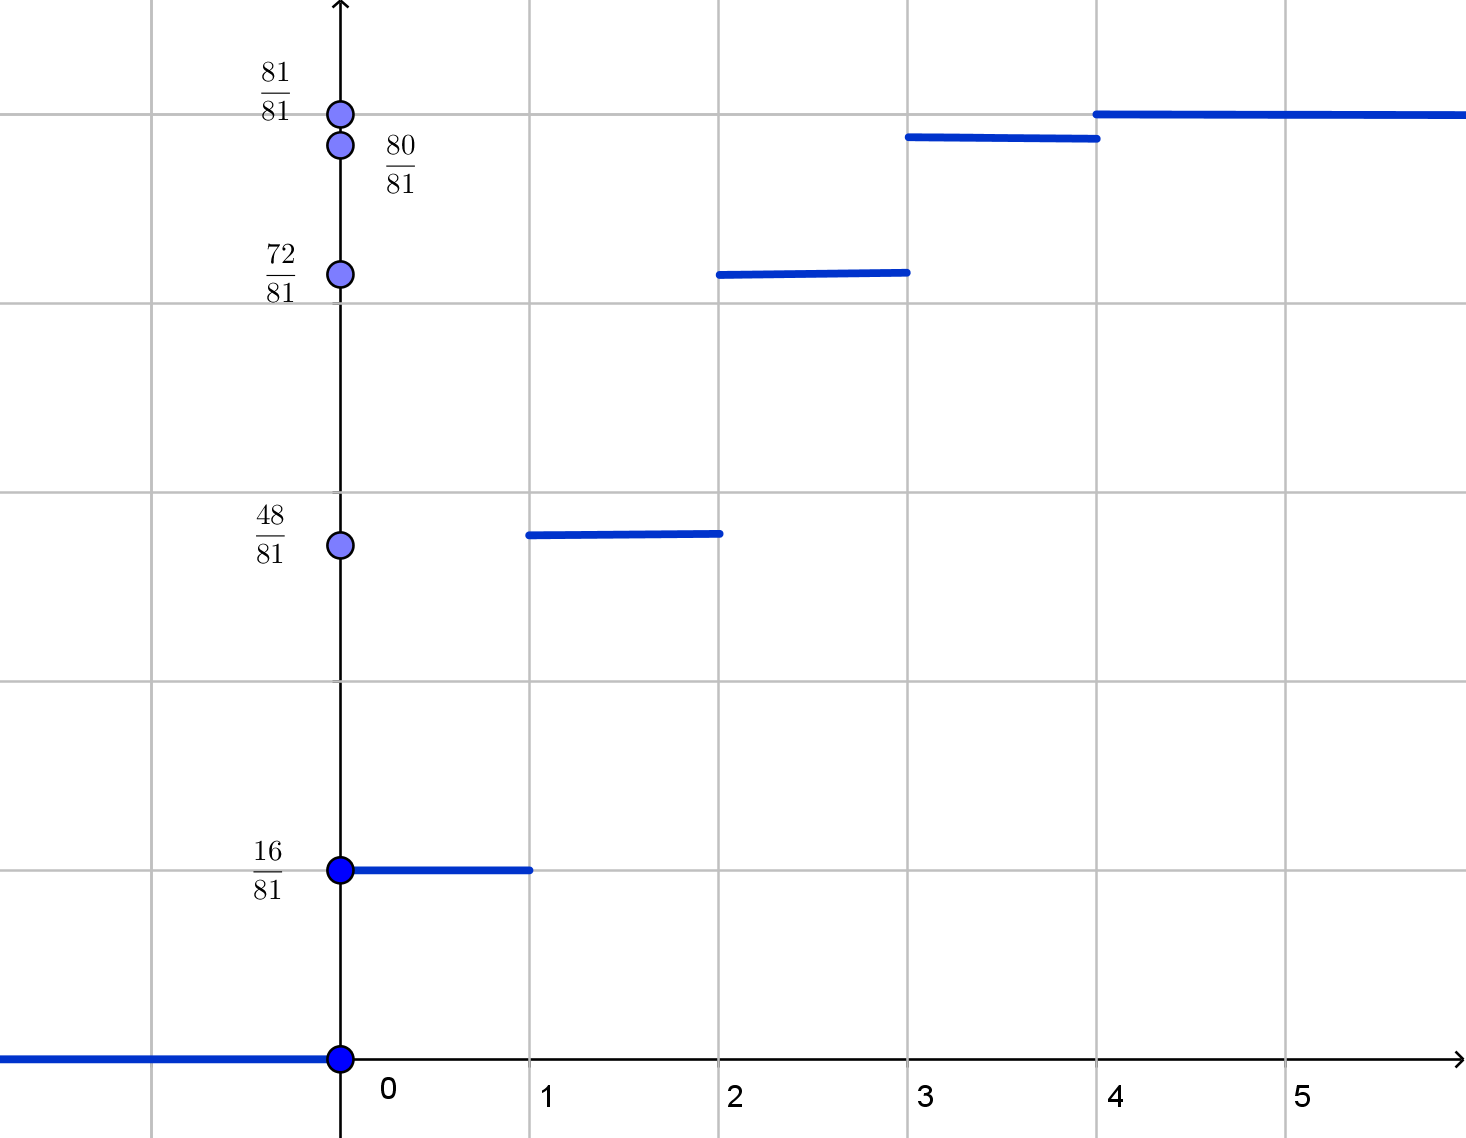
\includegraphics[width=80mm]{images/kr1_2017_3.png}
    }
    \caption{Функция распределения}
    \label{cdf_kr2017}
\end{figure}

\item Все вероятности посчитаны, видим, что наибольшая достигается при $\xi=1$.
\item $\E(X) = np = \frac{4}{3} $, $ \Var(X) = npq = \frac{8}{9}$
\end{enumerate}
\item
\begin{enumerate}
\item Так как указано, что цена сметаны распределена равномерно на отерзке $[250, 1000]$, максимальное значение цены — $1000$, это и есть необходимая сумма.
\item Вспомним, что функция распределения $F(x) = \P(X \leq x)$, нужно найти такой $x$, что $ \P(X \leq x)=0.9$:
\[
0.9 = 1 - \exp({-x^{2}}) \Rightarrow \exp(-x^{2}) = 0.1 \Rightarrow -x^2 = \ln(0.1)  \Rightarrow x=  \sqrt{-\ln(0.1)}
\]
\item Взяв производную от функции распределения списка без сметаны, получим функцию плотности:
\[
f_X(x) =
\begin{cases}
2x\exp(-x^2) & x \ge 0 \\
0 & \text{иначе}
\end{cases}
\]
Найдём математическое ожидание:
\[
\int_{0}^{+\infty}2x^2\exp({-x^2}) dx = -x \exp({-x^2})\big|_0^{+\infty} + \int_{0}^{+\infty}\exp({-x^2}) dx = \frac{\sqrt{\pi}}{2}
\]
\item Математическое ожидание суммы случайных величин равно сумме математических ожиданий случайных влечин, если они существуют. Математическое ожидание от цены сметаны равно: $ \frac{1000 + 250}{2} = 625 $
Математическое ожидание списка без сметаны было найдено в предыдущем пункте, его осталось перевести в рубли. Получаем ответ: $ 625 + \frac{\sqrt{\pi}}{2} \cdot 1000 $.
\item Так как обе величины имеют абсолютно непрерывные распределения, вероятность попасть в конкретную точку равна нулю.
\end{enumerate}
\item
\begin{enumerate}
\item $\P(\text{детектор показл ложь и подозреваемый лжёт}) = 0.9 \cdot 0.1 + 0.1 \cdot 0.95 = 0.185$
\item $\P(\text{невниовен}|\text{детектор показал ложь}) = \frac{0.9\cdot0.1}{0.185} = \frac{90}{185}$
\item $\P(\text{эксперт точно выявит преступника}) = (0.9)^9 \cdot 0.95$
\item $\P(\text{эксперт ошибочно выявит преступника}) = 9 \cdot 0.1 \cdot 0.9^8\cdot 0.05$
\end{enumerate}


%\item
%$\P(Ложь|Лжёт) = 0.95 $

%$\P(Ложь|Не лжёт) = 0.1 $

%$\P({Лжёт}) = \frac{1}{10} $

%\P(\text{Не лжёт}) = \dfrac{9}{10} $

%\begin{enumerate}
%	\item
%	По формуле полной вероятности: \[  \P(Ложь) = 0.95 \cdot 0.1 + 0.1 \cdot 0.9 = 0.185 \]
%	\item
%	По формуле Байеса: \[ \P(\text{Не лжёт}|Ложь) = \dfrac{0.1 \cdot 0.9}{0.185} = 0.486\]
%    \item
%    Событие "эксперт точно выявит преступника" соответствует событию "эксперт выявит, что лгун лжет, и      что остальные говорят правду".  Таким образом:  \[ \P = 0.1 \cdot 0.95 + 0.9 \cdot 0.9  = 0.905\]
%    \item
%    Это означает, что эксперт выберет 8 человек из 9 невиновных и скажет, что они говорят правду
%    (количество вариантов выбрать так людей  $С_9^8$ ), а также выберет 1 виновного и скажет, что он
%    говорит правду (количество вариантов это сделать 1), и выберет одного невиновного и скажет, что он
%    лжет (количество вариантов выбрать так человека $С_9^1$ ). Просуммируем все с учетом вероятностей,
%    указанных в условии: \[ \P = с_9^8 \cdot 0.9 \cdot 0.9 \cdot C_9^1 \cdot 0.9 \cdot 0.1 \cdot 1 \cdot 0.1
%    \cdot 0.05 = 0. 26244\]

%\end{enumerate}
\end{enumerate}



\subsection{Контрольная работа 1, ИП, 24.10.2017}


Ровно 272 года назад императрица Елизавета повелела завезти во дворцы котов для ловли мышей.


\begin{enumerate}

\item В отсутствии кота Леопольда мыши Белый и Серый подкидывают по очереди игральный додекаэдр
%\footnote{Леопольд подсказывает по случаю праздника, что у додекаэдра 12 граней :)}
.
Сыр достаётся тому, кто первым выкинет число 6. Начинает подкидывать Белый.

\begin{enumerate}
  \item Какова вероятность того, что сыр достанется Белому?
  \item Сколько в среднем бросков продолжается игра?
  \item Какова дисперсия числа бросков?
\end{enumerate}

\item Микки Маус, Белый и Серый решили устроить труэль из любви к мышки Мии. Сначала стреляет Микки, затем Белый, затем Серый, затем снова Микки и так до тех пор, пока в живых не останется только один.

Прошлые данные говорят о том, что Микки попадает с вероятностью $1/3$, Белый — с вероятностью $2/3$, а Серый стреляет без промаха.

Найдите оптимальную стратегию каждого мыша.

\item Микки Маус, Белый и Серый пойманый злобным котом Леопольдом до начала труэли. И теперь Леопольд будет играть с ними в странную игру.

В комнате три закрытых внешне неотличимых коробки: с золотом, серебром и платиной. Общаться после начала игры мыши не могут, но могут заранее договориться о стратегии.

Правила игры таковы. Кот Леопольд будет заводить мышей в комнату по очереди. Каждый из мышей может открыть
две коробки по своему выбору. Перед следующим мышом коробки закрываются.

Если Микки откроет коробку с золотом, Белый
— с серебром, а Серый — с платиной, то они выигрывают. Если
хотя бы один из мышей не найдёт свой металл, то Леопольд их съест.
\begin{enumerate}
\item Какова оптимальная стратегия?
\item Какова вероятность выигрыша при использовании оптимальной стратегии?
\end{enumerate}

\item Накануне войны Жестокий Тиран Мышь очень большой страны издал указ. Отныне за каждого новорождённого мыша-мальчика семья получает денежную премию, но если в семье рождается вторая мышка-девочка, то всю семью убивают. Бедные жители страны запуганы и остро нуждаются в деньгах, поэтому в каждой семье мыши будут появляться до тех пор, пока не родится первая мышка-девочка.

\begin{enumerate}
  \item Каким будет среднее число детей в мышиной семье?
  \item Какой будет доля мышей-мальчиков в стране?
  \item Какой будет средняя доля мышей-мальчиков в случайной семье?
  \item Сколько в среднем мышей-мальчиков в случайно выбираемой семье?
\end{enumerate}

\item Вальяжный кот Василий положил на счёт в банке на Гаити один гурд. Сумма на счету растёт непрерывно с постоянной ставкой в течение очень длительного промежутка времени. В случайный момент этого промежутка кот Василий закрывает свой вклад.

Каков закон распределения первой цифры полученной Василием суммы?

\begin{comment}
\item Начинающий трейдер Афанасий совершает не более одной сделки в день.

Если в какой-то день у трейдера Афанасия есть акция, то за этот день он равновероятно продаёт или не продаёт её. Если в какой-то день у трейдера Афанасия нет акций, то он равновероятно покупает или не покупает одну акцию.

Найдите ожидаемую прибыль Афанасия, если известно, что реализовывал он свою стратегию 100 дней, в начале акции стоили по 50 рублей, в конце — по 80 рублей, максимум составил 120 рублей, а минимум — 30.


\item Страшный Мейн-кун разрубает палочку единичной длины на $10$ частей в случайных и независимых местах, равномерно распределённых по всех длине. Затем Страшный Мейн-кун выбирает случайно один из кусочков и возводит его длину в $24$ степень.

Какое в среднем число он получит?
\end{comment}



\subsection{Контрольная работа 1, ИП, 24.10.2017, решения}


\begin{enumerate}

\item[1.]

\begin{enumerate}
	\item Обозначим вероятность того, что сыр достанется Белому за $b$, если игра начинается с его броска. Получаем уравнение
\[
	b = \frac{1}{12} + \frac{11}{12} \frac{11}{12} b
\]

Пояснение: Как Белый может победить в исходной игре? Либо сразу выкинуть 6 с вероятностью $1/12$. Либо передать ход Серому ($11/12$), получить ход снова ($11/12$) и выиграть в продолжении игры. Продолжение игры по сути совпадает с исходной игрой.

\item Игра продолжается до тех пор, пока кто-то не выкинет «6». Для нахождения среднего количества бросков воспользуемся методом первого шага.

Обозначим среднее количество бросков нашей игры за $S$. Когда Белый бросает кубик, с вероятностью $\frac{1}{12}$ игра закончится за один бросок, а с вероятностью $\frac{11}{12}$ игра продолжится и ход перейдёт к Серому. Но та игра, которая начнётся, когда бросать будет Серый, ничем не отличается от предыдущей, поэтому среднее количество бросков в ней будет равно $S$. Однако мы попадём в эту игру, «потратив» один бросок. Таким образом мы получаем:

\[
S = \frac{1}{12} \cdot 1 + \frac{11}{12}(S +1)
\]

Получается, что $S = 12$, значит игра длится в среднем 12 бросков.
\end{enumerate}

\item[3.]

Для того, чтобы выжить, мышам нужно ещё до начала игры договориться о стратегии, которая позволит им с наибольшей вероятностью открыть нужные сундуки. Если хотя бы две мыши выберут одинаковый сундук, то их в любом случае съедят. Поэтому одной из оптимальных стратегий будет ещё до начала игры мышам договориться и назвать левый сундук золотым, сундук посередине серебряным, а правый — платиновым. Каждый мышонок должен открыть тот сундук, в честь которого назван необходимый ему металл. Если внутри он обнаруживает свой металл, то он выбирает этот сундук, если внутри находится не тот металл, мышонок открывает тот сундук, на который указывает лежащий внутри предмет.

Например, первым заходит Микки Маус. Он открывает золотой (левый) ящик. Если внутри лежит золото, то он выходит из комнаты. Если же внутри лежит, например, серебро, то Микки Маус открывает сундук посередине. Путём несложного перебора можно посчитать, что в 4 случаях из 6 мыши смогут найти нужный металл, поэтому вероятность выигрыша при данной стратегии равна $\frac{2}{3}$.

\item[5.]

Функция распределения дохода кота Василия, положившего один гурд на вклад, представляется в виде $m_t = 1\cdot e^{rt}$, где $r$ — процентная ставка, а $t$ — прошедшее время. Момент закрытия вклада Т равномерно распределён на отрезке от 0 до $a$, который очень велик, поэтому сумма, которую получит Василий, представима в виде $Z = e^{Y}$, где $Y \sim v[0; ra]$.

Вероятность того, что первая цифра будет равна 1, равна вероятности того, что доход Василия будет лежать в пределах от 1 до 2 гурдов, плюс вероятность того, что он лежит в пределах от 10 до 20 гурдов и т.д. Таким образом, можно представить эту вероятность, как:
\[
\P(N=1) = \P(e^Y \in [1;2) ) + \P(e^Y \in [10; 20) ) + \ldots
\]

Это выражение можно преобразовать таким образом:
\[
\P(N=1) = \P(Y \in [\ln 1; \ln2) ) + \P(Y \in [\ln 10; \ln 20) ) + \ldots
\]

Так как Y — равномерно распределённая величина, то $\P(Y \in [\ln 1; \ln2) ) = \frac{\ln 2 - \ln 1}{ra}$. Для последующих слагаемых вероятность рассчитывается таким же образом. Воспользовавшись свойством логарифма, можно заметить, что $\frac{\ln 20 - \ln 10}{ra} = \frac{\ln 2}{ra}$. Поэтому вероятность того, что на первом месте суммы вклада стоит единица, равна $n\cdot \frac{\ln 2}{ra}$, где $n$ -- количество слагаемых. Путём аналогичных рассуждений получаем, что вероятность того, что на первом месте стоит двойка, равна $n\cdot \frac{\ln 3- \ln 2}{ra}$. Из-за того, что $a$ велико, можно считать, что число слагаемых одинаково.

Т.к. на первом месте обязательно будет находиться какая-то цифра, то сумма вероятностей будет равна 1. Получаем:
\[
\dfrac{n}{ra}(\ln \frac{2}{1} + \ln \frac{3}{2} + \ldots + \ln \frac{10}{9}) = 1
\]

Таким образом $\frac{n}{ra} = \frac{1}{\ln 10}$. Получается, что вероятность того, что на первом месте стоит единица, равна:
\[
\P (N=1) = \dfrac{\ln 2}{\ln 10}
\]

Закон распределения первой цифры выводится сложением соответствующих вероятностей.


\end{enumerate}




\end{enumerate}


\end{document}
